%   D O C U M E N T   P R E A M B L E
% Specify the document class, default style attributes, and page dimensions, etc.
% For hyperlinked PDF, suitable for viewing on a computer, use this:
\documentclass[letterpaper,12pt,titlepage,oneside,final,usenames,dvipsnames]{book}
 
% For PDF, suitable for double-sided printing, change the PrintVersion variable below to "true" and use this \documentclass line instead of the one above:
%\documentclass[letterpaper,12pt,titlepage,openright,twoside,final]{book}

% Some LaTeX commands I define for the document nomenclature.
\newcommand{\die}[2]{\frac{\partial #1}{\partial #2}}
\newcommand{\package}[1]{\textbf{#1}} % package names in bold text
\newcommand{\cmmd}[1]{\textbackslash\texttt{#1}} % command name in tt font 
\newcommand{\href}[1]{#1} % does nothing, but defines the command so the print-optimized version will ignore \href tags (redefined by hyperref pkg).
%\newcommand{\texorpdfstring}[2]{#1} % does nothing, but defines the command
% Anything defined here may be redefined by packages added below...
% This package allows if-then-else control structures.
\usepackage{ifthen}
\newboolean{PrintVersion}
\setboolean{PrintVersion}{false}
% CHANGE THIS VALUE TO "true" as necessary, to improve printed results for hard copies by overriding some options of the hyperref package, called below.

%\usepackage{nomencl} % For a nomenclature (optional; available from ctan.org)
\usepackage{amsmath,amssymb,amstext} % Lots of math symbols and environments
\usepackage[pdftex]{graphicx} % For including graphics N.B. pdftex graphics driver 

%----------------------------------------------------------------------
%   A D D  H E R E
% Packages added for Kirsten's dissertation
% \usepackage{geometry}
\usepackage{changepage}
\usepackage{epigraph}
\setlength\epigraphwidth{.8\textwidth}
\usepackage[absolute]{textpos}
% \usepackage{setspace}
\usepackage{xcolor}

\usepackage{listings}

\definecolor{codegreen}{rgb}{0,0.6,0}
\definecolor{codegray}{rgb}{0.5,0.5,0.5}
\definecolor{codepurple}{rgb}{0.58,0,0.82}
\definecolor{backcolour}{rgb}{0.95,0.95,0.92}

% Code style examples 
% https://github.com/srinadhu/RL_Pacman/blob/master/report.pdf
% https://www.overleaf.com/learn/latex/Code_listing

\lstdefinestyle{mystyle}{
    language=Python,
    backgroundcolor=\color{backcolour},   
    commentstyle=\color{codegreen},
    keywordstyle=\color{magenta},
    numberstyle=\tiny\color{codegray},
    stringstyle=\color{codepurple},
    basicstyle=\ttfamily\footnotesize,
    breakatwhitespace=false,         
    breaklines=true,                 
    captionpos=b,                    
    keepspaces=true,                 
    numbers=left,                    
    numbersep=5pt,                  
    showspaces=false,                
    showstringspaces=false,
    showtabs=false,                  
    tabsize=2
}

\lstset{style=mystyle}

% \definecolor{dkgreen}{rgb}{0,0.6,0}
% \definecolor{gray}{rgb}{0.5,0.5,0.5}
% \definecolor{mauve}{rgb}{0.58,0,0.82}
% \lstset{frame=tb,
%   language=Java,
%   aboveskip=3mm,
%   belowskip=3mm,
%   showstringspaces=false,
%   columns=flexible,
%   basicstyle={\small\ttfamily},
%   numbers=none,
%   numberstyle=\tiny\color{gray},
%   keywordstyle=\color{blue},
%   commentstyle=\color{dkgreen},
%   stringstyle=\color{mauve},
%   breaklines=true,
%   breakatwhitespace=true,
%   tabsize=3
% }

% \newcommand\pythonstyle{\lstset{
% language=Python,
% basicstyle=\ttm,
% morekeywords={self},              % Add keywords here
% keywordstyle=\ttb\color{deepblue},
% emph={MyClass,__init__},          % Custom highlighting
% emphstyle=\ttb\color{deepred},    % Custom highlighting style
% stringstyle=\color{deepgreen},
% frame=tb,                         % Any extra options here
% showstringspaces=false
% }}

% \usepackage{epstopdf}
\usepackage{catchfilebetweentags}
\usepackage{rotating} %DRR Sidewayas
\DeclareGraphicsRule{.tif}{png}{.png}{`convert #1 `dirname #1`/`basename #1 .tif`.png}
\usepackage{pgfplots}
\usepackage{tikz}
\usetikzlibrary{shadings, shadows, shapes, arrows, calc, positioning, shapes.geometric, arrows.meta}
%\usepackage[dvipsnames]{xcolor}
%\setpalette("R4")
%----------------------------------------------------------------------

% Hyperlinks make it very easy to navigate an electronic document.
% In addition, this is where you should specify the thesis title and author as they appear in the properties of the PDF document.
% Use the "hyperref" package 
% N.B. HYPERREF MUST BE THE LAST PACKAGE LOADED; ADD ADDITIONAL PKGS ABOVE
\usepackage[pdftex,pagebackref=false]{hyperref} % with basic options
%\usepackage[pdftex,pagebackref=true]{hyperref}
		% N.B. pagebackref=true provides links back from the References to the body text. This can cause trouble for printing.
\hypersetup{
    plainpages=false,       % needed if Roman numbers in frontpages
    unicode=false,          % non-Latin characters in Acrobat’s bookmarks
    pdftoolbar=true,        % show Acrobat’s toolbar?
    pdfmenubar=true,        % show Acrobat’s menu?
    pdffitwindow=false,     % window fit to page when opened
    pdfstartview={FitH},    % fits the width of the page to the window
%    pdftitle={uWaterloo\ LaTeX\ Thesis\ Template},    % title: CHANGE THIS TEXT!
%    pdfauthor={Author},    % author: CHANGE THIS TEXT! and uncomment this line
%    pdfsubject={Subject},  % subject: CHANGE THIS TEXT! and uncomment this line
%    pdfkeywords={keyword1} {key2} {key3}, % list of keywords, and uncomment this line if desired
    pdfnewwindow=true,      % links in new window
    colorlinks=true,        % false: boxed links; true: colored links
    linkcolor=blue,         % color of internal links
    citecolor=green,        % color of links to bibliography
    filecolor=magenta,      % color of file links
    urlcolor=cyan           % color of external links
}
\ifthenelse{\boolean{PrintVersion}}{   % for improved print quality, change some hyperref options
\hypersetup{	% override some previously defined hyperref options
%    colorlinks,%
    citecolor=black,%
    filecolor=black,%
    linkcolor=black,%
    urlcolor=black}
}{} % end of ifthenelse (no else)

\usepackage[automake,toc,abbreviations]{glossaries-extra} % Exception to the rule of hyperref being the last add-on package
% If glossaries-extra is not in your LaTeX distribution, get it from CTAN (http://ctan.org/pkg/glossaries-extra), 
% although it's supposed to be in both the TeX Live and MikTeX distributions. There are also documentation and 
% installation instructions there.

% Setting up the page margins...
% uWaterloo thesis requirements specify a minimum of 1 inch (72pt) margin at the
% top, bottom, and outside page edges and a 1.125 in. (81pt) gutter margin (on binding side). 
% While this is not an issue for electronic viewing, a PDF may be printed, and so we have the same page layout for both printed and electronic versions, we leave the gutter margin in.
% Set margins to minimum permitted by uWaterloo thesis regulations:
\setlength{\marginparwidth}{0pt} % width of margin notes
% N.B. If margin notes are used, you must adjust \textwidth, \marginparwidth
% and \marginparsep so that the space left between the margin notes and page
% edge is less than 15 mm (0.6 in.)
\setlength{\marginparsep}{0pt} % width of space between body text and margin notes
\setlength{\evensidemargin}{0.125in} % Adds 1/8 in. to binding side of all 
% even-numbered pages when the "twoside" printing option is selected
\setlength{\oddsidemargin}{0.125in} % Adds 1/8 in. to the left of all pages when "oneside" printing is selected, and to the left of all odd-numbered pages when "twoside" printing is selected
\setlength{\textwidth}{6.375in} % assuming US letter paper (8.5 in. x 11 in.) and side margins as above
\raggedbottom

% The following statement specifies the amount of space between paragraphs. Other reasonable specifications are \bigskipamount and \smallskipamount.
\setlength{\parskip}{\medskipamount}

% The following statement controls the line spacing.  
% The default spacing corresponds to good typographic conventions and only slight changes (e.g., perhaps "1.2"), if any, should be made.
\renewcommand{\baselinestretch}{1} % this is the default line space setting

% By default, each chapter will start on a recto (right-hand side) page.
% We also force each section of the front pages to start on a recto page by inserting \cleardoublepage commands.
% In many cases, this will require that the verso (left-hand) page be blank, and while it should be counted, a page number should not be printed.
% The following statements ensure a page number is not printed on an otherwise blank verso page.
\let\origdoublepage\cleardoublepage
\newcommand{\clearemptydoublepage}{%
  \clearpage{\pagestyle{empty}\origdoublepage}}
\let\cleardoublepage\clearemptydoublepage

% Define Glossary terms (This is properly done here, in the preamble and could also be \input{} from a separate file...)
% Main glossary entries---definitions of relevant terminology

% \newglossaryentry{}
% {
% name=,
% description={}
% }
% \newglossaryentry{}
% {
% name=,
% description={}
% }
% \newglossaryentry{}
% {
% name=,
% description={}
% }
% \newglossaryentry{}
% {
% name=,
% description={}
% }

\newglossaryentry{margin}
{
name=margin,
description={edge or boundary. In economics the term has an expanded metaphorically supported technical usage. Ricardo referred to the \gls{extensive margin} as the geographical limit of production and emphasised that that limit was the limit of profitable cultivation. It was where a sensible person would stop expanding the area of cultivation for economic reasons. Later economists extended the notion to the stopping point for all kinds of decisions. Using calculus they identified the conditions under which going farther adding more const more than it added.  Margin   appeared as a metaphor in the adjective  \gls{marginal} and in compound terms like \gls{marginal product}, where it refers to the effect of a small change on some variable  such as a small increase in output  from a small increase fertilizer or labour employed. Focus on such quantities is the main feature of the \gls{marginalist} approach. }
}

\newglossaryentry{consumer surplus}
{
name=consumer surplus,
description={}
}

\newglossaryentry{excess profits}
{
name=excess profits,
description={}
}

\newglossaryentry{free entry}
{
name=free entry,
description={}
}

\newglossaryentry{the second circuit of capital}
{
name=the second circuit of capital,
description={}
}

\newglossaryentry{producer surplus}
{
name=producer surplus,
description={}
}

\newglossaryentry{marginalism}
{
name=marginalism,
description={see \gls{marginalist}}
}

\newglossaryentry{produit net}
{
name=produit net,
description={Profit from a sale after having deducted the costs and charges related to the manufacture and marketing of a product.}
}

\newglossaryentry{competitive}
{
name=competitive,
description={See \gls{perfect competition}.}
}

\newglossaryentry{commodity}
{
name=commodity,
description={1) Any product  made for exchange on the market; 2) a basic good used in commerce that is interchangeable with other goods of the same type, usually  as inputs to the production of other goods or services; 3) raw materials or primary agricultural products.}
}

\newglossaryentry{marginalist}
{
name=marginalist,
description={A style of economic analysis that emphasizes marginal values as opposed to total values or average values. The significance of the distinction lies in the fact maximizing a function like the profit function or utility gives rise to expression in terms of marginal quantities like marginal cost, marginal revenue, and marginal utility. It is then possible to say a person wishing to maximize their profit or utility should want to satisfy the derived conditions on marginal values (prescription). Another step allows economists to assume that those conditions are likely to be satisfied (description). The style of argument generally relies on the use of calculus. The systematic shift to marginalist analysis is seen as the dividing line between classical and modern economics.}
}

\newglossaryentry{profit}
{
name=profit,
description={The amount retained from sale of a product after all costs including the normal cost of capital  been paid. This amount is the income of the enterprise. The normal cost of capital is thought of a price paid to the investors who lent their capital to the enterprise and must be paid as  much for its use as they would have received if they had lent to another project. }
}

\newglossaryentry{surplus value}
{
name=surplus value,
description={See \gls{surplus} and \dots value?}
}

\newglossaryentry{pseudo-rent}
{
name=pseudo-rent,
description={A term for profits used by Alfred Marshall to emphasize that profits are a form of rent, but differ in being subject to competitions  because capital, unlike land, is a produced input and is therefor only scarce in the short term. }
}

\newglossaryentry{scarcity}
{
name=scarcity,
description={}
}

\newglossaryentry{spatial rent}
{
name=spatial rent,
description={ See \gls{locational rent}}
}

\newglossaryentry{quasi-rent}
{
name=quasi-rent,
description={}
}

\newglossaryentry{Henry George Theorem}
{
name=Henry George Theorem,
description={A proof by Arnott and Stiglitz \cite{arnottAggregateLandRents1979} of the proposition that  that if economic activity is efficiently organized over a "large" space, aggregate land rents equal the aggregate losses from the decreasing returns to scale activities. In other words, consistent with the assertions of Henry George, under certain circumstances the \gls{single tax} would finance all the infrastructure costs of a city. }
}

\newglossaryentry{ground rents}
{
name=ground rents,
description={ all economic value accruing to owners of land, regardless of whether payments are explicitly made or the rents are imputed.}
}

\newglossaryentry{single tax}
{
name=single tax,
description={a tax on land and resources that Henry George and his followers suggest is capable of replacing all other taxes since, if properly implemented,it would capture all resource rents. }
}

\newglossaryentry{digitization}
{
name=digitization,
description={The process. of converting stored information to digital form or the processof replacing human mental and physical actions with digital processing and digitally directed actions. }
}

\newglossaryentry{market}
{
name=market,
description={a means by which the exchange of goods and services takes place as a result of buyers and sellers being in contact with one another, either directly or through mediating agents or institutions.}%Britannica
}

\newglossaryentry{landowner}
{
name=landowner,
description={the class of people who receive income from their ownership of land. Usually reserved for those who receive all or most of their income from land ownership and who do not work their land themselves.}
}

\newglossaryentry{working class}
{
name=working class,
description={In Classical and Marxist theory, the category of people who had only their labour to sell were called working class}
}


\newglossaryentry{petite bourgeoisie}
{
name=petty bourgeoisie,
description={a French term that refers to a social class composed of semi-autonomous peasants and small-scale merchants. They are characterized by their ownership of small amounts of productive capital - land or property and equipment.}
}

\newglossaryentry{classical rent}
{
name=classical rent,
description={This term is sometimes used to refer to Ricardos definition of rent ans the value of the original newt productivity of land, as distinct from rental price for a property or the more general notion of economic rent. See \gls{classical rent theory}, or \gls{economic rent}.}
}

\newglossaryentry{economic rent}
{
name=economic rent,
description={is any payment to the owner of a factor of production in excess of the cost needed to bring that factor into production. In classical economics, economic rent is any payment  or benefit received for non-produced inputs such as location  and through creating official privilege over natural opportunities. See \gls{rent}}
}

\newglossaryentry{locational rent}
{
name=locational rent,
description={Income or payment for the use of location. Locational value is largely created by access to people not by landowners, hence any payment for locational advantages is a rent. See \gls{rent} or \gls{land rent}.}
}

\newglossaryentry{land rent}
{
name=land rent,
description={Ricardo payment for  the natural productivity of the land, but also considered proximity to markets (locational advantages) as a source of rent. }
}

\newglossaryentry{intensive margin}
{
name=intensive margin,
description={Distinguished from the \gls{extensive margin}, which is a locational concept. Intensive refers to  enhancing the productivity of  the land by adding labour, fertilizers or other inputs, i.e. by intensifying cultivation efforts.  The intensive margin refers to the maximum intensity of additional factors of production that makes sense economically. }
}

\newglossaryentry{extensive margin}
{
name=extensive margin,
description={A term from Ricardian rent theory that refers to either land at the greatest distance from the market or land that has the minimum fertility that justifies bringing them into commercial production. A feature of land at the margin is that it generates no \gls{economic rent}. }
}

\newglossaryentry{generalized arithmetic mean}
{
name=generalized arithmetic mean,
description={ a family of functions for aggregating sets of numbers. One special case is the geometric mean,  and the Cobb-Douglas function is a special case of that. Wikipedia provides a \href{https://en.wikipedia.org/wiki/Generalized_mean}{useful discussion}. }
}

\newglossaryentry{transmission mechanism}
{
name=transmission mechanism,
description={A general term to describe the sequence of processes through which an action at one point in a system  affects a variable at another point in the system. It is commonly used when discussing  monetary policy and how  expanding the money supply eventually affects employment.}
}

\newglossaryentry{real asset}
{
name=real asset,
description={Real assets are physical assets that have an intrinsic worth due to their substance and properties. Real assets include precious metals, commodities, real estate, land, equipment, and natural resources. }
}

% % Do we want to just make this feedback loop and feedback cycle and make uses in glossary consistent?

\newglossaryentry{feedback}
{
name=feedback,
description={The result of a causal loop. A term used in cybernetics and systems theory referring to a situation in which a change in one variable affects a second variable that then affects the first one.}
}

\newglossaryentry{surplus}
{
name=surplus,
description={Any amount or production or value in excess of what  is needed to pay for all the required inputs. Profit or rent. }
}

\newglossaryentry{Ricardian rent theory}
{
name=Ricardian rent theory,
description={The version of classical rent theory propounded by David Ricardo in his essay on the corn laws and generally seen as the  canonical version of land rent theory.}
}

\newglossaryentry{land market}
{
name=land market,
description={The entire complex of institutions, agents, and rules involved in transferring ownership of land. A land market exists wherever it is possible to exchange rights in land for agreed amounts of money or services rendered.}
}

\newglossaryentry{Alonso-Jacobs cycle}
{
name=Alonso-Jacobs cycle,
description={A positive \gls{feedback} cycle that occurs when city population is increasing in the wage, as in the Alonso model, where the wage is increasing in city population, as implied by the Jacobs component of the \gls{Alonso-Jacobs model}.}
}

\newglossaryentry{Public-Private Partnerships}
{
name=Public-Private Partnerships,
description={A long-term arrangement between a government and private sector institutions, often  employed for building, equipping, operating and maintaining schools, hospitals, transport, water, and sewerage systems. PPPs are used for projects with high social but low private returns when government is unwillling or unable to provide the up-front capital cost. The private rate of return is often subsidized by a guarantee that the private investor will receive a share of the social return over the course of the project's operation.}
}

\newglossaryentry{rent-seeking}
{
name=rent-seeking,
description={An economic concept that refers to the activity, seeking to gain wealth without contributing to productivity. Gordon Tullock, who introduced  the term, identified it as a form of theft\cite{tullockWelfareCostsTariffs1967}.  %Rent-seeking is the act of growing one's existing wealth without creating new wealth by manipulating the social or political environment. 
\Gls{rent-seeking} activities have negative effects on the rest of society. They result in reduced economic efficiency through misallocation of resources, reduced wealth creation, lost government revenue, heightened income inequality.}
}

\newglossaryentry{middle class}
{
name=middle class,
description={A broad and fuzzy term used by sociologists to describe the members of the working classes who have equity and a standard of living above the subsistence level. The OECD includes anyone who earns between 75 per cent and 200 percent of median household income after tax. Based on the most recent data available from Statistics Canada, in this country that means anywhere from about \$45,000 to \$120,000. The middle class is usually defined in terms of income level. The middle class defined this way, once the economic stratum of a clear majority of North American adults, has steadily contracted in the past five decades according to
Rakesh Kochhar and  Stella Sechopoulos of the \href{https://www.pewresearch.org/fact-tank/2022/04/20/how-the-american-middle-class-has-changed-in-the-past-five-decades/}{Pew Research Centre}  in 2022.}
}

\newglossaryentry{rentier}
{
name=rentier,
description={A person living on income from property or investments rather than from current income. The term is from the  French \textit{rentier}, ``holder of rental properties or investments that pay income,'' from \textit{rente} ``profit, income'' \cite{GET_rentier_defn_quote}. %``Financial engineering has created a rentier class, a modern feudal system, and the biggest beneficiaries of all that extra debt have been the bankers.'' Times, Sunday Times (2016) 
}
}

\newglossaryentry{rate of return}
{
name=rate of return,
description={or return on investment: the money made or lost on an investment over some period of time. Expressed nominally as the change in dollar value of an investment over time or  as a percentage derived from the ratio of profit to investment. We compute the nominal return, convert it to a percentage and compare that to the investor's best alternative return or required return.}
}

\newglossaryentry{joint-stock company}
{
name=joint-stock company,
description={A joint-stock company is a business owned by its investors, with each investor owning a share of the company based on the amount that they've invested. It is a predecessor to the modern-day corporation and other types of registered companies. A joint-stock company is an artificial person; it has legal existence separate from persons composing it. It can sue and can be sued in its own name. The shareholders are usually not liable for any of the company debts that extend beyond the company's ability to pay up to the amount of them.}
}

\newglossaryentry{REIT}
{
name=REIT,
description={Real Estate Investment Trust. A REIT is a financial instrument that  makes it possible for individual investors to earn dividends from real estate investments without having to buy, manage, or finance properties themselves. Structured as a company that owns and sometimes operates income-producing real estate or related assets, REITs are modeled after mutual funds \cite[GET-reit-like-mortgages].} %cite REITs are modeled after mutual funds? 
}

\newglossaryentry{financial instrument}
{
name=financial instrument,
description={A financial instrument is a monetary contract, which confers a right or claim against some counterparty in the form of a payment (checks, bearer instruments), equity ownership or dividends (stocks), debt (bonds, loans, deposit accounts), currency (foreign exchange or forex), or derivatives (futures, forwards, options, and swaps). There are %\href{https://www.investopedia.com/terms/f/financialinstrument.asp}{many types} 
many types of financial instrument \cite[WEB-investment-types].}
}

\newglossaryentry{compound interest rate}
{
name=compound interest rate,
description={Where an interest rate is specified for a single term, such as a year, the rate for a longer, multi-period term is larger. If the calculation for a later period includes interest on the interest from earlier periods, the interest is said to ``compound.'' This is how interest is usually charged. Compound interest for a given period is calculated by multiplying the initial principal amount by one plus the annual interest rate raised to the number of compound periods minus one.}
}

\newglossaryentry{amortize}
{
name=amortize,
description={to reduce an amount gradually by making payment in installments: a to pay off (as a loan) gradually usually by periodic payments of principal and interest. }
}

\newglossaryentry{appraised value}
{
name=appraised value,
description={an evaluation of a property's value based on a given point in time. The evaluation is performed by a professional appraiser during the mortgage origination process.}
}

\newglossaryentry{premium}
{
name=premium,
description={The difference between the base price and the price paid in a particular market or buy a particular buyer. In our model is is the difference between the wage of rural workers and the wage of urban workers required to induce workers to live in the city and incur commuting costs. See \gls{urban wage},\gls{urban wage premium}, \gls{rent premium}.}
}

\newglossaryentry{subsistence frontier}
{
name=subsistence frontier,
description={The minimum income or lowest standard of living that can sustain people in the economy. Rather than thinking of the limit as a single value---say the minimum survival income---it is more realistic to recognize that the limit can be achieved with different combinations of goods. For example, if clean water is freely available in a local stream, the subsistence income does not include the cost of bottled water. All the combinations can be seen as a \gls{frontier}. \newline In classical economics, the frontier was summarized as a subsistence wage. Subsistence theorists like Malthus argued that the market price of labour would not vary from the natural price for long: if wages rose above subsistence, the number of workers would increase and bring the wage rates down. The classical economist recognized that the limit was in part set by social convention, but it was analytically convenient to assume a subsistence wage, and it could be argued, following Malthus that a subsistence wage  represented a long-term limit or \gls{equilibrium}. As an analytical convenience in our model, we employ a subsistence wage that includes housing and a conventional standard of living.  }
}

\newglossaryentry{political economy}
{
name=political economy,
description={Political economy is a branch of social science that studies the relationship  between government and the economy. As a discipline, it dates back the  16$^{th}$ but is usually associated with the political economists of the mid-18$^{th}$ and  early 19$^{th}$  century like Adam Smith who began to explore the economic implications of free markets and industrialization. Departments of political economy persisted well into the mid 20$^{th}$ C before splitting into separate departments of economics politics \cite{helleiner20PoliticalEconomy2018}.}
}

\newglossaryentry{expected market price}
{
name=expected market price,
description={The price is expected to emerge in a \gls{market} at a future point in time as a result of the interaction of buyers and sellers. It may vary as the mixture of buyers and sellers changes or as their information changes.}
}

\newglossaryentry{market price}
{
name=market price,
description={The price that emerges in a \gls{market} as a result of the interaction of buyers and sellers. It may vary as the mixture of buyers and sellers changes or as their information changes.}
}

\newglossaryentry{expectation}
{
name=expectation,
description={in our model, an agent's estimate of an unobserved or future value of a variable such as price. In simple statistical analysis the expectation of a variable may be taken as the average of the previously observed values.  }
}

% \newglossaryentry{perfect}
% {
% name=perfect,
% description={}
% }

\newglossaryentry{total factor productivity}
{
name=total factor productivity,
description={total-factor productivity (TFP), also called multi-factor productivity, is usually measured as the ratio of aggregate output  to aggregate inputs. It is a scale factor used to explain why the same combination of inputs produces different quantities of output at different places or times. It appears the factor  $A$ discussed in Chapter~\ref{chapter-growth} and in cities is influenced by the size of the population.  }
}

\newglossaryentry{factor of production}
{
name=factor of production,
description={(such as labour, land, financial capital,  and human capital)}
}

\newglossaryentry{perfect competition}
{
name= perfect competition,
description={An imaginary but analytically useful ideal market condition with the following  characteristics: 1. Large numbers of buyers and sellers in each market so that no individual buyer or seller can affect the price. 2. Free entry and exit of firms in the market. 3. Firms in each market sell a homogeneous product. 4. Buyers and sellers possess complete knowledge of the market. 5. No price controls.\newline  Economists often compare the markets they study to the` idealized, perfectly competitive market structure.}
}

\newglossaryentry{frontier}
{
name=frontier,
description={In mathematical economics, the limit of what is possible. Like the frontier of a country, even if you can't cross it, you can move along it to find the best location  subject to that constraint. In elementary economics, the budget-line and the production possibilities frontier (PPF) are  frontiers. Tf you spend less than the budget are operating inside the PPF, you could do better. Your solution is inefficient. }
}

\newglossaryentry{attractor}
{
name=attractor,
description={In \gls{dynamical system} theory as described by difference or differential equations, an attractor is a point or orbit inside a region of the phase space. The phase space is a representation of all possible states of the system each corresponding to a unique point in the phase space. If there is an attractor in the region, if the system starts at any point in the region,  it will eventually evolve to the attractor.}
}

\newglossaryentry{dynamical system}
{
name=dynamical system,
description={any system that changes over time. Typically we mean a  system that is described by a set of interrelated equations, one of which is time-dependent. }
}

\newglossaryentry{agent-based}
{
name=agent-based,
description={a term for a model that is a  collection of autonomous decision-making entities called agents. In practice the agents are little sub-programs (automata, robots) that each separately use some information about their environment and follow some internal rules to choose a response in each model cycle. See \gls{agent-based model}}
}

\newglossaryentry{price formation}
{
name=price formation,
description={The process of selecting a price based on the conditions in a system. The classic problem is the simple supply and demand model, in which sellers and buyers, each group with its own wants represented by an equation, interact to find a a price. The model  identifies a combination of price and quantity that would be acceptable to both at the same time, but doesn't say how they get to the price. It lacks a price formation mechanism.  \newline The fundamental problem is that the agents don't have complete information and may have limited computational ability, especially with multiple interacting markets. A theory of price formation has to describe the process of adjustment. This is usually represented as a set of individual adjustment rules, which makes any theory of price formation a dynamical system It may not always lead to a steady state equilibrium.}
}

\newglossaryentry{classical}
{
name=classical,
description={Referring to the period of economic theorizing primarily in Britain roughly between 1750 and 1870, prior to the neoclassical period in economics. See \gls{classical economics}.   }
}

\newglossaryentry{market rent}
{
name=market rent,
description={The amount a landlord charges a tenant for the use of a property in a competitive market. }
}

\newglossaryentry{mill rate}
{
name=mill rate,
description={The municipal tax rate: the amount per \$1,000 of the assessed value of a property which will be due as property tax.}
}

\newglossaryentry{financialization}
{
name=financialization,
description={Something is financialized when a financial instrument representing it is created. The  home mortgage market was financialized when financial institutions developed markets that let let investors buy and sell mortgages between themselves. These transactions gave investors ownership of the stream of income established by the mortgage contract. The transaction did not affect the mortgage conditions or the home: they simply added a new product for investors to speculate on. }
}

\newglossaryentry{amenity}
{
name=amenity,
description={a desirable or useful feature or facility of a building or place.}
}

\newglossaryentry{population}
{
name=population,
description={In our model, the number of city residents. }
}

\newglossaryentry{financialize}
{
name=financialize,
description={Something is financialized when a financial instrument representing it is created. For example, mortgages originated in England when people did not have the resources to purchase land in one transaction. Buyers would get loans directly from the seller---no banks or outside parties were involved. Home mortgages were financialized when financial institutions developed markets that let them buy and sell mortgages between themselves.  See \gls{financialization}}
}

\newglossaryentry{housing market}
{
name=housing market,
description={A market is defined as the sum total of all the buyers and sellers engaged in the transfer of ownership of an asset, good or service, plus all of the institutional machinery that supports the transactions. }
}

\newglossaryentry{urban center}
{
name=urban center,
description={In our model the urban centre is a point at the center of a population agglomeration where all employment is located. More generally it is the area within an urban agglomeration with with the largest  concentration of employment and or commercial activities.} 
}

\newglossaryentry{functional form}
{
name=functional form,
description={the algebraic form of a relationship between a dependent variable and explanatory variables.}
}

\newglossaryentry{production}
{
name=production,
description={The process of converting a set of \glspl{input} into a desired \gls{output}. See\gls{factor of production}.}
}

\newglossaryentry{perfectly elastic}
{
name=perfectly elastic,
description={Producing more won't affect the product's price. The term describes a  horizontal supply or demand curve. See \gls{elasticity}.} % On a \gls{supply demand curve} (is that the right name?) ***}
}

\newglossaryentry{elasticity}
{
name=elasticity,
description={The ratio of the percentage change in a quantity to the percentage change in another quantity. The price elasticity of demand, for  example, would be the percentage change in the quantity demanded that accompanies a one-percent change in price. It is a (local) property of a demand curve and would typically be a negative number like $-0.3$ or $-1.5$, since demand typically slopes downward. See \gls{perfectly elastic}.}
}

\newglossaryentry{labour augmenting agglomeration}
{
name=labour augmenting agglomeration,
description={The situation in which bringing more workers together increases their average productivity.}
}

\newglossaryentry{present discounted value}
{
name=present discounted value,
description={The amount that someone should be willing to pay, in the present, for a stream of expected future payments.}
}

\newglossaryentry{wealth}
{
name=wealth,
description={In our model, wealth is the set of valuable economic resources owned, by an individual or organization as measured in either real goods or money value, that the bank considers in lending decisions. We model only housing and aggregate financial wealth (savings), but more generally, wealth includes stocks of human capital, equities, land, and other more subtle assets.}
}

\newglossaryentry{input}
{
name=input,
description={In production theory, an input is any good or service used to produce another another good or service. % anything  that is among the collections of goods and services that is used to produce a desire  product or service. 
For example, labour is a necessary input for producing food. }
}

\newglossaryentry{output}
{
name=output,
description={In production theory, an output anything produced.} % Often symbolized by $Y$ or $Q$  in relations like $Y= F(K,L,N)$.}
}

\newglossaryentry{subsistence wage}
{
name=subsistence wage,
description={In most urban models the subsistence wage is treated as base cost that is the opportunity cost of agricultural land. We have extended the technique to include the opportunity cost of urban labour. It is one of the simplifications which makes our model tractable and focuses it on the question of rents and the specifically urban productivity premium. In our model, the subsistence wage is a wage available inside and outside the urban area, which covers the cost of buildings, food, core living costs, and a base cost of land.}
}

\newglossaryentry{urban wage premium}
{
name=urban wage premium,
description={The wage premium is the premium above the \gls{subsistence wage} payed by employers to attract workers. An urban wage premium appears when workers in larger cities earn higher average wages than workers in smaller cities. In both the U.S. and Sweden a wage premium has been shown to follow a power-law relationship that scales superlinearly with city size. In other words, workers in larger cities not only earn higher average wages, they do so systematically as a power law function of the size of the city. Bettencourt  \cite{bettencourtIntroductionUrbanScience2021}, has demonstrated theoretically that a wage premium should manifest as a power law function and predicted the value of its exponent.}
}

\newglossaryentry{urban wage}
{
name=urban wage,
description={The \gls{urban wage} is the \gls{urban wage premium} plus the \gls{subsistence wage}.}
}

\newglossaryentry{product}
{
name=product,
description={A product is anything produced. It is an \gls{output} of a production process. % Our model has no specific products. 
Rather than specific products, the city in our model produces an aggregate output, which is not a variable in our analysis. Instead of producing explicit list of discrete products, output is defined by an implicit production function relating labour as an input to aggregate productivity and thus to wages. % as part of urban incomes.
}
}

\newglossaryentry{imperfect competition}
{
name=imperfect competition,
description={A market in which any of the conditions required for \gls{perfect competition} are not met.}
}



\newglossaryentry{demand function}
{
name=demand function,
description={An equation describing how much a potential buyer or group of buyers will purchase at any given price. It can express price as a function of quantity or quantity as a function of price. In either case it will usually include other variables that are said to "shift" demand.   }
}

% \newglossaryentry{supply demand curve}
% {
% name=supply demand curve,
% description={}
% }

\newglossaryentry{increasing returns to scale}
{
name=increasing returns to scale,
description={a property of a production process  such that that when all the inputs are increased in the same proportion, the quantity of \gls{output} increases by a greater proportion.}
}

\newglossaryentry{decreasing returns to scale}
{
name=decreasing returns to scale,
description={a property of a production process  such that that when all the inputs are increased in the same proportion, the quantity of \gls{output} increases by a lesser proportion.}
}

\newglossaryentry{constant returns to scale}
{
name=constant returns to scale \gls{CRS}. ***,
description={a property of a production process such that that when all
the \glspl{input}s are increased in the same proportion, the quantity of \gls{output} increases by the same proportion.  }
}

\newglossaryentry{equilibrium condition}
{
name=equilibrium condition,
description={A condition that must be satisfied if a resultant variables of the system are to remain constant. ``For an equilibrium of prices and quantities in normal free \gls{market}, supply must equal demand.''}
}

\newglossaryentry{population equilibrium}
{
name=population equilibrium,
description={an \gls{equilibrium condition} that ensures population will not rise or fall  for the region under consideration. In urban model it is the condition that people cannot make themselves better off by moving to another location in the system. Formally it can be expressed by the requirement that the utility of people with the same  assets and tastes is equal at every location. }
}

\newglossaryentry{urban labour supply}
{
name=urban labour supply,
description={in our model this is simply the urban population, but more generally it is all those in the general population willing to work at the location or occupation.}
}

\newglossaryentry{stochastic}
{
name=stochastic,
description={Having a random probability distribution or pattern that may be analyzed statistically but may not be predicted precisely. Introducing even a small amount of random nose into even one variable in a model of a deterministic system converts the model into a stochastic model.}
}

\newglossaryentry{aggregate}
{
name=aggregate,
description={Formed or calculated by the combination of many separate units or items; a total.}
}

\newglossaryentry{agglomeration economies}
{
name=agglomeration economies,
description={Economic efficiencies resulting from \gls{agglomeration effects}.}
}

\newglossaryentry{agglomeration}
{
name=agglomeration,
description={A collection of similar items in one location. A city is an agglomeration of people and generally of firms. Agglomeration may have properties that individuals do not have, giving rise to \gls{agglomeration effects} or gls{agglomeration economies}.}
}

\newglossaryentry{locational equilibrium}
{
name=locational equilibrium,
description={A situation in which no resident will make herself better off by moving to another location. A Nash equilibrium with housing efficiently allocated  given market prices. See \gls{migration equilibrium}.}
}

\newglossaryentry{agglomeration effects}
{
name=agglomeration effects,
description={An effect of increasing the number of firms  or workers in one place. A larger, deeper, more specialized labour pool enables workers to better match their skills to the needs of firms or creates knowledge spillovers in which firms and workers learn from each other.}
}

\newglossaryentry{monopolistic competition}
{
name=monopolistic competition,
description={A type of  \gls{imperfect competition}. \gls{Perfect competition} is a description of a market with many seller, all of whom are price-takers. Monopoly is a market with a single seller, who therefore has the power to set the selling price. Monopolistic competition describes cases in between, with sellers that have some power to set prices within a segment of the market. It occurs when many companies offer competing products or services that are similar, but are not perfect, substitutes.}
}

\newglossaryentry{labour adjustment cost}
{
name=labour adjustment cost,
description={Costs associated with hiring, firing or training that prevent or slow the rate at which a firm will increase or decrease the number of workers it employs.}
}

\newglossaryentry{frictional unemployment}
{
name=frictional unemployment,
description={the part of total unemployment  due to people being in the process of voluntarily moving from one job to another.}
}

\newglossaryentry{marginal product}
{
name=marginal product,
description={the amount that the last unit of any factor  adds to output while holding all other factors constant. See \gls{marginal product of labour}.}
}

% \newglossaryentry{marginal product of labour}
% {
% name=marginal product of labour,
% description={Firms calculate what the next worker is worth to them. That's what they're willing to pay for labour. 
% This is the labour \gls{demand function} based on the \gls{marginal product} which is declining. When a firm has only a few workers, it is high on that demand function, and has to move down. It cuts workers. If it's too low, it expands and hires. %This says something about the geometry of what employers could pay. 
% % Firms can't pay workers more than they can earn in the long term, unless that money comes from somewhere, but they could push down wages and extract more profit, invest more in other factors of production, etc.
% }
% }

\newglossaryentry{marginal product of labour}
{
name=marginal product of labour (MPL),
description={the amount that the last worker  adds to output without changing the quantities of other inputs used. The firm's \gls{demand function} for labour in a competitive market is identically  the \gls{marginal product} of labour function, represented as a downward sloping curve due to the diminishing marginal productivity of labour. See \gls{marginal}.}
}

\newglossaryentry{monopoly}
{
name=monopoly,
description={ Market power means you can price above marginal costs. Need free entry to get rid of it---it doesn't drive out profit---profits can be sustained over longer. Monopolist can charge a higher price but pays a competitive price for all \glspl{input} including labour. If a firm also had a monopoly on offering jobs, they could drive down wages.}
}

\newglossaryentry{duopoly}
{
name=duopoly,
description={A market with two sellers. Under one set of assumptions the result will be the monopoly price, under others, the situation will generate lower  than monopoly prices, ore even competitive pricing and may result in market instability.}
}

\newglossaryentry{monopsony}
{
name=monopsony,
description={A market with one buyer who therefore has some power to determine the purchase price by varying the quantity purchased. An example of \gls{imperfect competition}.}
}

\newglossaryentry{imperfect information}
{
name=imperfect information,
description={ the buyers and/or sellers do not have all the information necessary to make an informed decision.}
}

\newglossaryentry{externalities}
{
name=externalities,
description={any indirect costs or benefit to uninvolved third parties that are an effect of a decision-makers activity but are not included in the decision-maker's cost-benefit calculations. Lawn mowers may wake the neighour, emissions from vehicles cause emphysema, burning fossil fuels may contribute to climate change, or painting your house may raise the value of the neighbour's house. In our model, when employers increase their workforce there is a positive effect on the productivity of all other workers in the city. This is an external effect}
}

\newglossaryentry{competitive market}
{
name=competitive market,
description={**FIX Everybody is a price taker. Price takers don't assume anything they do affects other producers or suppliers, so they act in terms of their internal prices and costs. 
This means their decision making process doesn't take into account any one else's behaviour.
? The easy way to see that is assume prices are fixed - all that's required to get the behaviour \dots  have a few other things like free exit and entry, perfect information etc---to get the efficiency result.} % (or to ensure price taking)}
}

\newglossaryentry{effective labour}
{
name=effective labour,
description={FIX - Effective labour is the productive \gls{output} from labour. As soon as you introduce agglomeration economies, labour becomes a more complex phenomena. There is the benefit of the single worker which should be perfectly declining on that nice concave production function and there is the diagonal movement as a result of increasing productivity because you keep adding people to the market. That means that your productivity of the worker isn't' just attached to the worker and your plant. It has this other component \dots 'effective labour'---the output including the A term.}
}

\newglossaryentry{spillover effects}
{
name=spillover effects,
description={ \Gls{externalities} are the most commonly discussed form of spillover effects but any economic event in one context that occurs because of something else in a seemingly unrelated context can be considered a spillover. It is a looser term than externality because an externality is a consequence, at least in economic theory, of rational optimizing behaviour.}
}

\newglossaryentry{substitutable}
{
name=substitutable,
description={One good may be substituted for another without loss of benefit. Two brands of motor oil are good substitutes for each other. Oranges are somewhat subsitutable for apples , but not for screwdrivers.}
}

\newglossaryentry{neoclassical distribution theory}
{
name=neoclassical distribution theory,
description={A theory that states that in perfect competition the owner of every unit of every  \gls{factor of production} will be paid precisely the  value of the \gls{marginal product} of that factor for each unit unit they contribute to production.}
}

\newglossaryentry{Solow-Swan model}
{
name=Solow-Swan model,
description={a  model of macro-economy developed and analysed by Robert Solow and Trevor Swan independently to explain long-run economic growth \cite{dimandTrevorSwanNeoclassical2009}. It attempts to explain  growth in terms of the growth of three contributing factors, capital, labor (population),  and  productivity.}
}



\newglossaryentry{migration equilibrium}
{
name=migration equilibrium,
description={The theoretical situation in which no resident can  make themselves better off by moving to another location. It is a logical consequence of utility maximization and free mobility that results in a Pareto optimal allocation of housing. Technically it is a Nash equilibrium, While extremely useful in analysing urban systems, the concept does not closely describe real cities.
% A situation in which not resident will make herself better off by migrating to or between cities or countries. Similar to a migration equilibrium.
}
}

\newglossaryentry{commuter shed}
{
name=commuter shed,
description={For a city, the area over which people will travel to work in a city. In the \gls{Alonso-Jacobs model}, it is sharply defined by the maximum distance commuters can travel before transportation costs exceed the wage premium. In  practice, the duration of commutes is highly variable. It is greater in the case of men, singles, educated and foreign workers, persons living in rented housing, using public transport, living or working in large cities, or working in large firms,  and when the  unemployment rate is high\cite{axisaFactorsInfluencingCommute2012} .}
}

\newglossaryentry{circular city}
{
name=circular city,
description={In urban theory, an idealized city form predicted by models with uniform travel costs in all directions and a fixed household commuting budget. If a city is laid out on a rectangular grid, the same travel-cost logic yields a rectangular city. Recently the term is applied to cities committed to achieving a circular economy. }
}

\newglossaryentry{radial city}
{
name=radial city,
description={A radial concentric city plan is formed by streets that extend outward from a defined center and reach the outer edge of the city, together with concentrically arranged roads that connect the radial streets to the lots. it is an idealized pattern that traces back to ancient times and appears  today in planned cities and districts. See \gls{circular city}.}
}

% \newglossaryentry{surplus}
% {
% name=surplus,
% description={Or economic surplus. Any social product in excess of the minimum required to reproduce society. In value terms the surplus appears as profit or rent and accrues to the owner of a  scarce \gls{input} that varys in quality, such as land. In the mid-19th century, French engineer Jules Dupuit first extended the concept of economic surplus to what came to be called producer- and consumer-surplus.}
% }

\newglossaryentry{Alonso-Jacobs model}
{
name=Alonso-Jacobs model,
description={A model combining the \gls{Alonso model} of the urban land use  \cite{alonsoModelUrbanLand1960} with the \gls{agglomeration} theory of Jane Jacobs \cite{jacobsEconomyCities1969} which explains the productivity of cities.}
}

\newglossaryentry{monopsonist}
{
name=monopsonist,
description={A single buyer, usually in an input market. A monopsonist is not a price-taker, knowing that buying more well result in  higher prices. This rleads the monopsonist to purchase less than is socially efficient.}
}

\newglossaryentry{financial return}
{
name=financial return,
description={MAYBE ADD what is best definition? - there may be other returns. Assessed by comparing the net rent $\mathcal{R}_N$ to the costs of acquiring a property, in particular to the cost of borrowing money. CLARIFY}
}

\newglossaryentry{home services}
{
name=home services,
description={A property offers two kinds of services: home services and \gls{locational services}. Home services describes the value offered by living in a house: a place to sleep, to prepare food, the amenity of being in the home, etc. Since people require housing inside and outside the city, home services are modeled as paid for as a share of the subsistence wage ($a \psi$).}
}

\newglossaryentry{locational services}
{
name=locational services,
description={A property offers two kinds of services: \gls{home services} and locational services. Locational services are services accessed by right of location. They include access to the central city job, access to locational amenity, and the benefit of services and connections associated with a location. In the core model, Locational services are, on an annual basis, the rent premium $w$, minus the transportation costs $c$ for a property a given distance, $d$, from the center, $\omega- {dc}$.}
}

\newglossaryentry{rent share}
{
name=rent share,
description={}
}

\newglossaryentry{Pareto efficiency}
{
name=Pareto efficiency,
description={An economic state where resources cannot be reallocated to make one individual better off without making at least one individual worse off.}
}

\newglossaryentry{efficiency conditions}
{
name=efficiency conditions,
description={Conditions derived in neoclassical economic theory that must be satisfied if a system or activity is to achieve Pareto efficiency. Under somewhat reasonable conditions the efficiency conditions are achieved by agents acting in a decentralized manner to maximize their own profit or utility.}
}

\newglossaryentry{neoclassical economics}
{
name=neoclassical economics,
description={An approach to the study of the economy and economic behaviour that attempts to explain the production, pricing, and the consumption of goods and services through supply and demand, and to explain agent behaviour using a theory of rational agents who satisfy \gls{marginal} efficiency conditions. It integrates, within a mathematical framework, the cost-of-production theory from classical economics with a consumer demand theory based on utility maximization.}
}


\newglossaryentry{neoclassical}
{
name=neoclassical,
description={refers to a period in economic theorizing that overlaps with  but largely follows classical economics and dominates economic theory to  today. See \gls{classical economics}, \gls{neoclassical economics}.}
}

\newglossaryentry{classical economics}
{
name=classical economics,
description={Also called classical \gls{political economy}. A school of thought in political economy that flourished, primarily in Britain, in the late 18th and early-to-mid 19th century. It was part of the intellectual  development of  Western liberal democracies in the 18th and 19th centuries and  brought into the mainstream by Scottish economist Adam Smith. Its main thinkers include Adam Smith, Jean-Baptiste Say, David Ricardo, Thomas Robert Malthus, and John Stuart Mill. After 1850, key features of the classical approach were carried forward by  Karl Marx and his followers, and by Henry George. Classical economics  provided the foundation for the development of \gls{neoclassical economics}.}
}

\newglossaryentry{socioeconomic status}
{
name=socioeconomic status,
description={Socioeconomic status is typically broken into three levels, high, middle, and low,  commonly referred to as ``upper class,'' ``middle class,'' and ``working or lower class,'' it differs from `\gls{class}' in the more traditional sense, which is a functional classification. See \gls{Ricardian class}, being based on occupation, income, family wealth.}
}

\newglossaryentry{Ricardian class}
{
name=Ricardian class,
description={The conception of class in \gls{classical economics} including Marx, where class is based on the types and amounts of productive capital the individual owns. See \gls{class}.}
}

\newglossaryentry{rent profile}
{
name=rent profile,
description={see \gls{bid-rent function} or \gls{bid-rent curve}}
}

\newglossaryentry{class}
{
name=class,
description={This term has a wide range of sometimes conflicting meanings. In our usage, which is consistent with classical economics including Marx, class is based on the types and amounts of productive capital the individual owns. This is a functional definition quite distinct from socioeconomic status which is more common in the current discussion. Our treatment of the evolution of class structure with financialization draws on We allow  people in different functional classes to own financial capital, producing intermediate classes \`a la Roemer\cite{roemerGeneralTheoryExploitation1982}.}
}
\newglossaryentry{capitalize}
{
name=capitalize,
description={To capitalize a stream of expected income is to compute it's capitalized value. Capitalized value is the current worth of an asset, usually real estate, based on a calculation of present value of expected income over the course of its economic lifespan.}
}

\newglossaryentry{agglomeration effect}
{
name=agglomeration effect,
description={The external economies associated with size and concentration. The benefits of size and concentration vary for different cross-sections of the urban population. Three such groupings may be identified: 1. Consumer agglomeration economies; Business agglomeration economies; Social agglomeration economies \cite{carlinoAgglomerationEconomiesSurvey1978}.}
}

\newglossaryentry{price bubble}
{
name=price bubble,
description={The sustained rise in the price of an asset above its ``normal'' market value'' caused by agents (mainly speculators) forecasting further price increases base on previous increases, rather than on estimates on intrinsic value.  Price bubbles are sustained by expectations of future increases in the price of an asset. They may end sharply, or crash, when expectations shift.}
}

\newglossaryentry{marginal value-product}
{
name=marginal value-product,
description={Also known as the marginal revenue product. The marginal revenue created due to an addition of one unit of productive resource, such as one more worker. Calculated by multiplying the marginal physical product by the price, or the marginal revenue in the case of a non-competitive market.}
}

\newglossaryentry{neoclassical growth theory}
{
name=neoclassical growth theory,
description={An economic theory that outlines how a steady economic growth rate results from a combination of three driving forces---labour, capital, and technology. Robert Solow and Trevor Swan developed and introduced the model of long-run economic growth in 1956. It is the  foundation of most empirical and theorical attempts to explain macroeconomic growth.}
}


\newglossaryentry{capital}
{
name= capital,
description={The word "capital" has many different meanings in economics and finance.  In economics, real capital is durable produced goods that are in turn used as productive inputs. \Gls{financial capital} is wealth that can be used to lend to others in exchange for interest payments or to purchase assets. Both these forms of capital are represented in the economy by extensive legal organizational structures that represent the interests of their owners. Other forms of capital recognized by economists are human capital, social capital natural capital, and intellectual capital. The distinctive  features of capital include that it takes time and energy to create (natural capital, however is  `a free gift of nature''), lasts a long time, deprecates, produces a stream of benefits over time,  and may be transferable as property}
}

\newglossaryentry{financial capital}
{
name=financial capital,
description={Financial capital is simply lendable purchasing power. Owners of financial capital provide their liquidity to borrowers in exchange for a future return. Interest rates are the prices charged for the use of financial capital. It is generally based on (secured by) ownership of tradable assets.  Anything can be a form of financial capital as long as it has a monetary value and can be  used in the pursuit of future revenue. Marx distinguished  financial capital (then called circulating capital or money capital) from fixed or real capital.}
}

\newglossaryentry{agent-based model}
{
name=agent-based model,
description={Agent-based models are computer simulations used to study the interactions between people, things, places, and time. They are usually stochastic models built from the `bottom up,' meaning by modelling individual agents (people, institutions, etc). Agents essentially sub-programs that respond to other agents and the environment in certain ways. These interactions produce emergent effects that may differ from the results of traditional, regression-based methods in that, like systems dynamics modeling, it allows for the exploration of complex systems that display non-independence of individuals and \gls{feedback} loops in causal mechanisms.}
}

\newglossaryentry{urban scaling}
{
name=urban scaling,
description={Urban scaling laws reliably relate socio-economic, behavioural and physical variables to the population size of cities. They allow for approaches  to city planning and for an understanding of urban resilience and economics. In this thesis we use the well-established relationship between population and urban productivity \cite{GET_doi:10.1098/rsif.2020.0705}}.
}

\newglossaryentry{classical rent theory}
{
name=classical rent theory,
description={explained how land generated surplus value for its owner and how this surplus explained the wealth and income of the land-owning class. David Ricardo produced the classic description in 1815 based on extensive prior analysis by others in the preceding century. The key notion is the ``marginal'' unit of land. It is just barely worth putting this land into production because it just barely produces enough to justify the cost of production, and transportation. More productive land or better located land produces a surplus that the landowner  collects in the form of land rent collected from tenant farmers. No tenant would pay to cultivate the  i unit of land. The theory employed the basic logic of later the later ``marginalist''  school of economic analysis. = See \gls{class}, \gls{rent}.}
}

\newglossaryentry{rent}
{
name=rent,
description={The economic  surplus generated in production as a result of differences in the quality of some \gls{factor of production}. Often described as the difference between the opportunity cost of a factor of production and the income it earns. In this thesis we focus on rents generated by \glspl{agglomeration effect}. According to \gls{classical rent theory}, rent is the price paid for the use of land. More generally it is the  surplus generated by any natural resource, up to and including the athletic talents of basketball stars \cite{lackmanClassicalBaseModern1976}. Land, talent, and mineral resources are seen as ``the free gift of nature,'' forms of capital which the owners do not create but do appropriate. Like the productivity of agricultural land in classical theory,  urban \gls{agglomeration effect}s produce land rents that are not created but are appropriated by the landowners. See \gls{class}.}
}

\newglossaryentry{maximum bid function}
{
name=maximum bid function,
description={A function that generates the maximum that an investor would bid for a property.  See \gls{bid-rent curve}, \gls{bid-rent function}.}
}

\newglossaryentry{bid-rent function}
{
name=bid-rent function ,
description={See \gls{bid-rent curve}.}
}

\newglossaryentry{reservation price}
{
name=reservation price,
description={Seller's minimum price of to accept a bid. If no offer is at least as large as the reservation price, the seller is effectively the buyer. It is lowest price that a prospective seller will accept, and is computed as seller's maximum bid price, which incorporates the net rent achievable.}
}

\newglossaryentry{bid-rent curve}
{
name=bid-rent curve,
description={The height of a graph showing distance from employment horizontally and the amount that residents will pay to rent land at that distance. It is also also called a \gls{rent profile}. With varying agents and property attributes can be seen a set of functions of location, each of which  generates a bid price for one category of agent.   See \gls{rent premium}, .}
}

\newglossaryentry{borrowing ratio}
{
name=borrowing ratio,
description={$m$. The maximum fraction of the price of a property that may be mortgaged. Determined by the bank (the lender) based on individual wealth and income. }
}

\newglossaryentry{rent premium}
{
name=rent premium,
description={or \gls{warranted economic rent} is the excess rent  that might be charge for the use of urban land relative the non-urban land. In our model the rent premium for an urban property is equal to the urban wage premium minus the transportation costs. }
}

\newglossaryentry{warranted rent}
{
name= warranted rent,
description={$\mathcal{R}_N$, at an  urban location  $d$ units from the centre, is the the value of the flow of services provided by the property, including the locational value, or \gls{warranted economic rent}. It is level of land rent that would be expected in equilibrium based on location and transportation costs.  (It may not be the rent actually charged to a tenant.) }
}

\newglossaryentry{warranted price}
{
name= warranted price,
description={, $P_W$, at an  urban location  $d$ units from the centre, \gls{capitalize}d value of the flow of services provided by the property, the \gls{warranted rent}.  
It   includes  the locational value, or \gls{warranted economic rent}, (It may differ from the market price) }}

\newglossaryentry{warranted economic rent}
{
name=warranted economic rent,
description={The locational value of an urban property. A surplus generated by \glspl{agglomeration effect}, equal to the urban (wage premium) minus transportation costs, $\omega-{c} d$). This is the the amount that an equilibrium market rent for a property would be expected to exceed the market rent for a similar non-urban property.}
}

\newglossaryentry{net rent}
{
name=net rent,
description={Or net market rent. The \gls{warranted rent} minus taxes and maintenance costs.}
}

% \newglossaryentry{rent share}
% {
% name=rent share,
% description={\dots}
% }

% rent paid
% economic rent
% locational rent

\newglossaryentry{marginal}
{
name=marginal,
description={relating to or situated at the edge or margin of something. In the marginalist approach to economics, it  refers to technique of focusing on the cost or benefit of the next unit or individual. See \gls{extensive margin}, \gls{intensive margin}, \gls{marginal product}, \gls{marginal value-product}, \gls{inframarginal}.}
}

\newglossaryentry{inframarginal}
{
name=inframarginal,
description={Coming before the margin is reached. For example, if the wage is $x$, all workers willing to work for less than $x$ are inframarginal. They are selling their time for more that it is worth to them. They come out ahead on the bargain. Workers who will work for $x$ but not a penny less are marginal. Similarly, with land, the most remote or the least productive land in use is ``marginal'' while  inframarginal land is more productive and generates a \gls{surplus}.}
}

\newglossaryentry{overlapping generations}
{
name=overlapping generations,
description={In the \gls{OLG} model individuals live a finite length of time, long enough to overlap with at least one period of another agent's life. The OLG model is the natural framework for the study of life-cycle behavior (investment in human capital, work and saving for retirement).}
}

\newglossaryentry{stylized facts}
{
name=stylized facts,
description={Economists use this term for observations that are widely understood to be empirical truths, to which theories must fit.  Also described as, ``broad tendencies that aim to summarize the data, offering essential truths while ignoring individual details.'' The term "stylized facts" was introduced by the economist Nicholas Kaldor in the context of a debate on economic growth theory in 1961 \cite{kaldorCapitalAccumulationEconomic1961}.}
}

\newglossaryentry{perfect foresight}
{
name=perfect foresight,
description={The correct prediction of future events. If agents have  all relevant information and  a correct model to use for prediction. When there is uncertainty it is not possible to have perfect foresight. In solving a complex intertemporal model, economists may assume agents have perfect foresight. This is called the rational expectations approach.}
}

\newglossaryentry{equilibrium reasoning}
{
name=equilibrium reasoning,
description={Gls{equilibrium} analysis identifies variable values of particular interest because they are likely to exhibit stability or capture the implications of the goals of agents. Using these equilibrium values and how they are likely to change in the regions of an equilibrium draw conclusions to is `equilibrium reasoning' because it bases the conclusions on assumptions about the behaviour of the variables near an equilibrium. Equilibrium reasoning implicitly  assumes that the variables will tend to stay near and smoothly approach the equilibrium.}
}

\newglossaryentry{equilibrium}
{
name=equilibrium,
description={In economics and other sciences, an equilibrium is a situation in which forces such as supply and demand are balanced, and in the absence of external influences the (equilibrium) values of variables will not change. In economics an equilibrium is usually understood behaviourally as a situation in which no agent has an incentive to change behaviour given what others are doing. Such a situation is called a Nash Equilibrium or a Cournot-Nash equilibrium.}
}

\newglossaryentry{expectations}
{
name=expectations,
description={Predictions of future events or values, formed by agents for use in decision-making. Agents may form their expectations by looking backward at data on previous values, or by projecting forward using a mental model of how the system works. If agents are fully informed about the state of the system and how it works, their expectations are essentially the same as the predictions of the relevant economic theory and they are termed `rational expectations' \cite{muthRationalExpectationsTheory1961}. In probability theory, the expected value of a variable is the mean of its true distribution (the rational expectation), which is usually estimated using the observed realizations (a backward-looking estimate).}
}

\newglossaryentry{Alonso model}
{
name=Alonso model,
description={The model credited to William Alonso, also called the Alonso-Muth model. A full development of the theory is presented in Alonso's doctoral dissertation \cite{alonsoTheoryUrbanLand1960}.} %, A MODEL OF THE URBAN LAND MARKET: LOCATIONS AND DENSITIES OF DWELLINGS AND BUSINESSES, University of Pennsylvania, 1960.}
}

\newglossaryentry{asking price}
{
name=asking price,
description={The price a seller initially posts on deciding to sell a property. It will be higher than the seller's maximum bid price.}
}

\newglossaryentry{bid price}
{
name=bid price,
description={In the computational model, any price that an agent bids for a property in the transaction process. It will be less than or equal to the agent's maximum bid price and less than or equal to the asking price.}
}

\newglossaryentry{maximum bid price}
{
name=maximum bid price,
description={The maximum price that investors will bid for a property. A bid that makes the expected return exactly the required or  target return.}
}

\newglossaryentry{bargaining}
{
name=bargaining,
description= {in the computational model during price setting for a particular property, there is a bargaining process that takes as arguments the highest bid price, reservation price, and asking price, returning a sale price for the property, as well as property transfer instructions.}
}
%The reservationn prices  is  the seller  own bid. If the max bid of the highest bid received is lower than the own bid the seller is the buyer- remains the owner. 
%Otherwisesimplest rule is  (reservation bid+maxbid)/2


\newglossaryentry{model}
{
name=model,
description={A system, A, which is useful for understanding another system, B. as the model we present is useful for understanding the effect of growing finacialization working through the system of urban land ownership.}
}

\newglossaryentry{specification}
{
name=specification,
description={With respect to a model or a theory, associating the theoretical constructs or relationships in a theory with a specific model, or associating specific model elements with observables.}
}

\newglossaryentry{distribution}
{
name=distribution,
description={The way total \gls{output}, income, \gls{wealth} or assets are distributed among individuals, each \gls{factor of production}, or the \glspl{class} of society. The term may refer to a theoretical approach  or to an empirical distribution of any of these. Theories of distribution are systematic attempts to account for the sharing of the national income.  Distributions across classes is known as a functional distribution distribution and  corresponds to the the approach of the \gls{classical economics}. Neoclassical economics examined distribution through the payment to factors of their \gls{marginal value-product}.}
}

\newglossaryentry{production function}
{
name=production function,
description={A representation of the technology of production, often a functional relationship between the \glspl{input} that enable production and the quantity of \gls{output}.}
}

\newglossaryentry{Cobb-Douglas}
{
name=Cobb-Douglas,
description={A specific production function. commonly used for illustrative or estimation in economics. Essentially a form of geometric mean.}
}

\newglossaryentry{productivity}
{
name=productivity,
description={The ratio of \gls{output} to \glspl{input}. Which outputs and inputs are considered varies. \gls{total factor productivity} refers to aggregate outputs and inputs in value terms. Marginal productivity refers to the addition to total output produced by one additional unit of input.} 
}

\newglossaryentry{growth}
{
name=growth,
description={The rate of increase in aggregate \gls{output} for a given production unit, such as a nation  or a city.}
}

\newglossaryentry{regime}
{
name=regime,
description={A distinct state of a system, a region of the system's phase space. In dynamical system theory, a phase space is a space in which all possible states of a system are represented, with qualitatively distinct  states corresponding to one region in the phase space.}
}

\newglossaryentry{resilience}
{
name=resilience,
description={The ability of a system to return to its original state when shocked by a change in its determining variables. May refer to smoothly or successfully adapting to a change in  determining variables.}
}

\newglossaryentry{hysteresis}
{
name=hysteresis,
description={An event in the economy that persists even after the factors that led to that event have been removed or otherwise run their course.}
}

\newglossaryentry{present value}
{
name=present value,
description={The value in cash today of a future sum of money or stream of cash flows, given a specified rate of return.}
}

\newglossaryentry{capital gain}
{
name=capital gain,
description={The difference between the future sale price and the current purchase price.}
}

\newglossaryentry{discount factor}
{
name=discount factor,
description={The present value of a dollar at a specified time in the future. It is a compounded value calculated using the individual discount rate.}
}

\newglossaryentry{mortgage term}
{
name=mortgage term,
description={The length time after a house purchase until a sum for a house purchase, the mortgage, must be returned to the lender with interest.}
}

\newglossaryentry{use value}
{
name=use value,
description={The monetary value of being allowed to live at a certain location ignoring potential speculative gains or losses.}
}

\newglossaryentry{wealth trajectories}
{
name=wealth trajectories,
description={A term for the people's  asset portfolios change over time. As their \gls{wealth} changes, an individual's \gls{class} position may change. For example, if a household is able to make  a down payment on a house,  the person's wealth will generally increase more rapidly than t the wealth of a person who does not purchase a house. The wealth trajectories differ. Savings out of labour income may enable a member of the \gls{working class} to move into the \gls{middle class} and enjoy income from his or her financial assets. The collection  of wealth trajectories at any time characterizes a society. Changes in the ensemble of wealth trajectories reflect the evolution and class structure of society.   } 
}

% % Nomenclature glossary entries---New definitions, or unusual terminology
% \newglossary*{nomenclature}{Nomenclature}
% \newglossaryentry{dingledorf}
% {
% type=nomenclature,
% name=dingledorf,
% description={A person of supposed average intelligence who makes incredibly brainless misjudgments}
% }

% List of Abbreviations (abbreviations type is built in to the glossaries-extra package)

% \newabbreviation{}{}{}
% \newabbreviation{}{}{}
% \newabbreviation{}{}{}
% \newabbreviation{}{}{}
% \newabbreviation{}{}{}
% \newabbreviation{}{}{}

% \newabbreviation{REIT}{REIT}{real estate investment trust}

\newabbreviation{ABM}{ABM}{agent-based model}

\newabbreviation{CRS}{CRS}{constant returns to scale}

\newabbreviation{OLG}{OLG}{overlapping generations}

% List of Symbols
\newglossary*{symbols}{List of Symbols}
\newglossaryentry{rvec}
{
name={$\mathbf{v}$},
sort={label},
type=symbols,
description={Random vector: a location in n-dimensional Cartesian space, where each dimensional component is determined by a random process}
}
\makeglossaries

%======================================================================
%   L O G I C A L    D O C U M E N T
% The logical document contains the main content of your thesis.
% Being a large document, it is a good idea to divide your thesis into several files, each one containing one chapter or other significant chunk of content, so you can easily shuffle things around later if desired.
%======================================================================

\begin{document}

%----------------------------------------------------------------------
% FRONT MATERIAL
% title page,declaration, borrowers' page, abstract, acknowledgements,
% dedication, table of contents, list of tables, list of figures, nomenclature, etc.
%----------------------------------------------------------------------
% % T I T L E   P A G E
% -------------------
\pagestyle{empty}
\pagenumbering{roman}

\begin{titlepage}
        \begin{center}
        \vspace*{1.0cm}

        \Huge
        {\bf Financialization of the Housing Market: A Contribution to Modern Urban Rent Theory}

        \vspace*{1.0cm}

        \normalsize
        by \\

        \vspace*{1.0cm}

        \Large
        Kirsten Wright \\

        \vspace*{3.0cm}

        \normalsize
        A thesis \\
        presented to the University of Waterloo \\ 
        in fulfillment of the \\
        thesis requirement for the degree of \\
        Doctor of Philosophy \\
        in \\
        Systems Design Engineering \\

        \vspace*{2.0cm}

        Waterloo, Ontario, Canada, 2023 \\

        \vspace*{1.0cm}

        \copyright\ Kirsten Wright 2023 \\
        \end{center}
\end{titlepage}

% The rest of the front pages should contain no headers and be numbered using Roman numerals starting with `ii'
\pagestyle{plain}
\setcounter{page}{2}

\cleardoublepage % Ends the current page and causes all figures and tables that have so far appeared in the input to be printed.
% In a two-sided printing style, it also makes the next page a right-hand (odd-numbered) page, producing a blank page if necessary.
\phantomsection    % allows hyperref to link to the correct page
 
% E X A M I N I N G   C O M M I T T E E (Required for Ph.D. theses only)
% Remove or comment out the lines below to remove this page
\addcontentsline{toc}{chapter}{Examining Committee}
\begin{center}\textbf{Examining Committee Membership}\end{center}
  \noindent
The following served on the Examining Committee for this thesis. The decision of the Examining Committee is by majority vote.
  \bigskip
  
  \noindent
\begin{tabbing}
Internal-External Member: \=  \kill % using longest text to define tab length
External Examiner: \>  Tara Vinodrai \\ 
\> Associate Professor, Department of Geography and Planning, \\
\> University of Toronto \\
\end{tabbing} 
  \bigskip
  
  \noindent
\begin{tabbing}
Internal-External Member: \=  \kill % using longest text to define tab length
Supervisor(s): \> Jangho Yang \\
\> Assistant Professor, Department of Management Science and \\ 
\> Engineering, University of Waterloo \\
\> Sean Geobey \\
\> Associate Professor, School of Environment, Enterprise and \\
\> Development, University of Waterloo \\
\end{tabbing}
  \bigskip

  \noindent
\begin{tabbing}
Internal-External Member: \=  \kill % using longest text to define tab length
Internal Member: \> Chrystopher Nehaniv \\
\> Professor, Department of Systems Design Engineering, \\
\> University of Waterloo \\
\end{tabbing}
  \bigskip

  \noindent
\begin{tabbing}
Internal-External Member: \=  \kill % using longest text to define tab length
Internal Member: \> Terry Stewart \\
\> Adjunct Professor, Department of Psychology, \\
\> University of Waterloo \\
\end{tabbing}
  \bigskip

  \noindent
  \begin{tabbing}
Internal-External Member: \=  Frances Westley \\ % \kill % using longest text to define tab length
% Internal Member: \> \\
\> Professor, School of Environment, Enterprise and Development, \\
\> University of Waterloo \\
\end{tabbing}
  \bigskip


  
%   \noindent
% \begin{tabbing}
% Internal-External Member: \=  \kill % using longest text to define tab length
% Other Member(s): \> Supervisor Name \\
% \> Professor, Dept. of Systems Design Engineering, University of Waterloo \\
% \end{tabbing}

\cleardoublepage
\phantomsection    % allows hyperref to link to the correct page

% D E C L A R A T I O N   P A G E
% -------------------------------
  % The following is a sample Declaration Page as provided by the GSO
  % December 13th, 2006.  It is designed for an electronic thesis.
 \addcontentsline{toc}{chapter}{Author's Declaration}
 \begin{center}\textbf{Author's Declaration}\end{center}
  
 \noindent
% I hereby declare that I am the sole author of this thesis. This is a true copy of the thesis, including any required final revisions, as accepted by my examiners.

  \bigskip
  
  \noindent
I understand that my thesis may be made electronically available to the public.

\cleardoublepage
\phantomsection    % allows hyperref to link to the correct page

% A B S T R A C T
% ---------------
\addcontentsline{toc}{chapter}{Abstract}

The dissertation posits two core hypotheses: firstly, that financialization induces a shift towards tenancy among the urban workforce. Secondly, that this results in decreased urban productivity due to the redirection of spatial rents away from local investments financialization disrupts the relationship between population growth and productivity, reducing the wealth and resilience of the urban system.

DONE WITH MODELS INCLUDE LIMITATIONS

Contributions of this dissertation include: integrating classical rent theory into an agent-based urban model; linking urban rent dynamics with urban productivity and population growth; incorporating urban scaling literature into the model framework; and examining the impacts of financialization on wealth distribution and urban productivity.


## Contributions:

0. Having understood what you mean by rent/by the implications of rent in an urban situation
1. First we put financialization into a model an agent based urban model that is well constrained and well understood, and show that in a plausibly specified model, the financialization is driving the change in the class structure. 
2. The economic literature does not examine the class impact. Economists don't talk about. Sociologists talk about it, but they don't model it.
3. We model boom bust dynamics/response. how it responds to changes in the outer world - fact you could get a change with an interest rate. what happens when the model is repeatedly struck. What are the impact effects and how do they play out?
4.  We ask the question about if there's a spillover to productivity. There's speculation about the link in the left win urban literature but we haven't found any modeling.

This is what's done in the climate literature. The dynamics and resilience effects are not obvious from the equations and must be modelled. The modeling is important because empirical dynamics are really hard to establish. This is a 1 off world. We can't run 50 versions. You can, however model 50 versions. 

The basic fiancialization result is clear from looking at the model. The equations only make it obvious once you put it together, however. They way they are combined is not obvious.  It is important to note also that the results are not a consequence of building a model that will give any result, but only a consequence of building a model that behaves urban theory and the economic theory predicts. None of the equations were constructed to give a result. Each is our best about how it works. Each step was a best guess at how the process works and based on a knowledge of the literature and the economics. The base theory in neither literature clearly predicts the class effects (there is some work in the literature e.g. Jacobs, reinvesting in Henry George literature - a few places where the economists have gone in that direction) We implemented a version of the best of the urban growth theories.

## Hypotheses
1. The financial sector affects the ownership of housing and the class structure of society, 
2. There are dynamic/resilience features of this model that make the effects worse
- Boom bust - pump wealth on/out of city on the boom and on the bust. 'There are sharks in the water' 1. Higher bid can amplify up swings - have to compete with speculators 2. can't get it back on down swing since outside finance offers a stable floor- buys up on way down (we expect larger effects as people are 1. displaced on the way up and then 2. evicted on the way down - can't use their spaces)
- Hysteresis - perturb, doesn't come back - e.g. interest rates go up.
- The way it aligns with long run changes in the landscape e.g. tech changing local info changes vulnerability to these shocks -- Depth of the basin changes - erodes systemic resilience - together these changes the capacity to hold value in landscape. (links to the productivity feedback - much will/can they invest in increasing their productivity/supporting kids/good food to grow brains. Education to increase productivity is the feature that makes productivity increases resilient to de-industrialization). This has implications for landscape/system/class structure.
3. This shift in ownership may have implications for urban productivity. (can actually displace productive uses - empty store fronts) - who can/will enter, how , who can rent spaces, speculative value may keep it empty (work spaces or living space - lowering pop), reduces consumption


\cleardoublepage
\phantomsection    % allows hyperref to link to the correct page

% A C K N O W L E D G E M E N T S
% -------------------------------
\addcontentsline{toc}{chapter}{Acknowledgements}
\begin{center}\textbf{Acknowledgements}\end{center}

I would like to thank all the people who made this thesis possible.
\cleardoublepage
\phantomsection    % allows hyperref to link to the correct page

% D E D I C A T I O N
% -------------------
\addcontentsline{toc}{chapter}{Dedication}
\begin{center}\textbf{Dedication}\end{center}

\begin{center}
To Wyatt, Jackie, and Jason.    
\end{center}

\cleardoublepage
\phantomsection    % allows hyperref to link to the correct page

% T A B L E   O F   C O N T E N T S
% ---------------------------------
\renewcommand\contentsname{Table of Contents}
\tableofcontents
\cleardoublepage
\phantomsection    % allows hyperref to link to the correct page

% L I S T   O F   F I G U R E S
% -----------------------------
\addcontentsline{toc}{chapter}{List of Figures}
{\renewcommand{\addvspace}[1]{} \listoffigures}
\cleardoublepage
\phantomsection		% allows hyperref to link to the correct page

% L I S T   O F   T A B L E S
% ---------------------------
\addcontentsline{toc}{chapter}{List of Tables}
{\renewcommand{\addvspace}[1]{} \listoftables}
\cleardoublepage
\phantomsection		% allows hyperref to link to the correct page

% L I S T   O F   A B B R E V I A T I O N S
% ---------------------------
\renewcommand*{\abbreviationsname}{List of Abbreviations}
\printglossary[type=abbreviations]
\cleardoublepage
\phantomsection		% allows hyperref to link to the correct page

% L I S T   O F   S Y M B O L S
% ---------------------------
\printglossary[type=symbols]
\cleardoublepage
\phantomsection		% allows hyperref to link to the correct page


% Change page numbering back to Arabic numerals
\pagenumbering{arabic}


% T I T L E   P A G E
% -------------------
\pagestyle{empty}
\pagenumbering{roman}

\begin{titlepage}
        \begin{center}
        \vspace*{1.0cm}

        \Huge
        {\bf Financialization of the Housing Market: A Contribution to Modern Urban Rent Theory}

        \vspace*{1.0cm}

        \normalsize
        by \\

        \vspace*{1.0cm}

        \Large
        Kirsten Wright \\

        \vspace*{3.0cm}

        \normalsize
        A thesis \\
        presented to the University of Waterloo \\ 
        in fulfillment of the \\
        thesis requirement for the degree of \\
        Doctor of Philosophy \\
        in \\
        Systems Design Engineering \\

        \vspace*{2.0cm}

        Waterloo, Ontario, Canada, 2024 \\

        \vspace*{1.0cm}

        \textcopyright{} Kirsten Wright 2024 \\ % Use \textcopyright instead of \copyright

        % \copyright\ Kirsten Wright 2024 \\
        \end{center}
\end{titlepage}

\pagestyle{plain}
\setcounter{page}{2}

% T A B L E   O F   C O N T E N T S
% ---------------------------------
\renewcommand\contentsname{Table of Contents}
\tableofcontents
\cleardoublepage
\phantomsection    % allows hyperref to link to the correct page

% L I S T   O F   F I G U R E S
% -----------------------------
\addcontentsline{toc}{chapter}{List of Figures}
{\renewcommand{\addvspace}[1]{} \listoffigures} % remove space between chapters
% \listoffigures
\cleardoublepage
\phantomsection		% allows hyperref to link to the correct page

% L I S T   O F   T A B L E S
% ---------------------------
\addcontentsline{toc}{chapter}{List of Tables}
{\renewcommand{\addvspace}[1]{} \listoftables} % remove space between chapters
% \listoftables
\cleardoublepage
\phantomsection		% allows hyperref to link to the correct page

% % L I S T   O F   A B B R E V I A T I O N S
% % ---------------------------
% \renewcommand*{\abbreviationsname}{List of Abbreviations}
% \printglossary[type=abbreviations]
% \cleardoublepage
% \phantomsection		% allows hyperref to link to the correct page

% % L I S T   O F   S Y M B O L S
% % ---------------------------
% \printglossary[type=symbols]
% \cleardoublepage
% \phantomsection		% allows hyperref to link to the correct page

% Change page numbering back to Arabic numerals
\pagenumbering{arabic}


%----------------------------------------------------------------------
% MAIN BODY
% We suggest using a separate file for each chapter of your thesis.
% Start each chapter file with the \chapter command.
% Only use \documentclass or \begin{document} and \end{document} commands in this master document.
% Tip: Putting each sentence on a new line is a way to simplify later editing.
%----------------------------------------------------------------------

\chapter{Introduction} \label{chapter-introduction}

% \vspace*{\fill}


%``cities..% the 'force' we need to postulate account for the central role of cities in economic life is of exactly the same character as the 'external human capital'}{Robert E. Lucas Jr., \textit{ON THE MECHANICS OF ECONOMIC DEVELOPMENT (1988)}}

\epigraph{Cities are the crucible of civilization, the hubs of innovation, the engines of wealth creation and centers of power, the magnets that attract creative individuals, and the stimulant for ideas, growth, and innovation.}{Geoffrey West}
% \cite{westScaleUniversalLaws2017}

\begin{figure}[!ht]
    \centering
    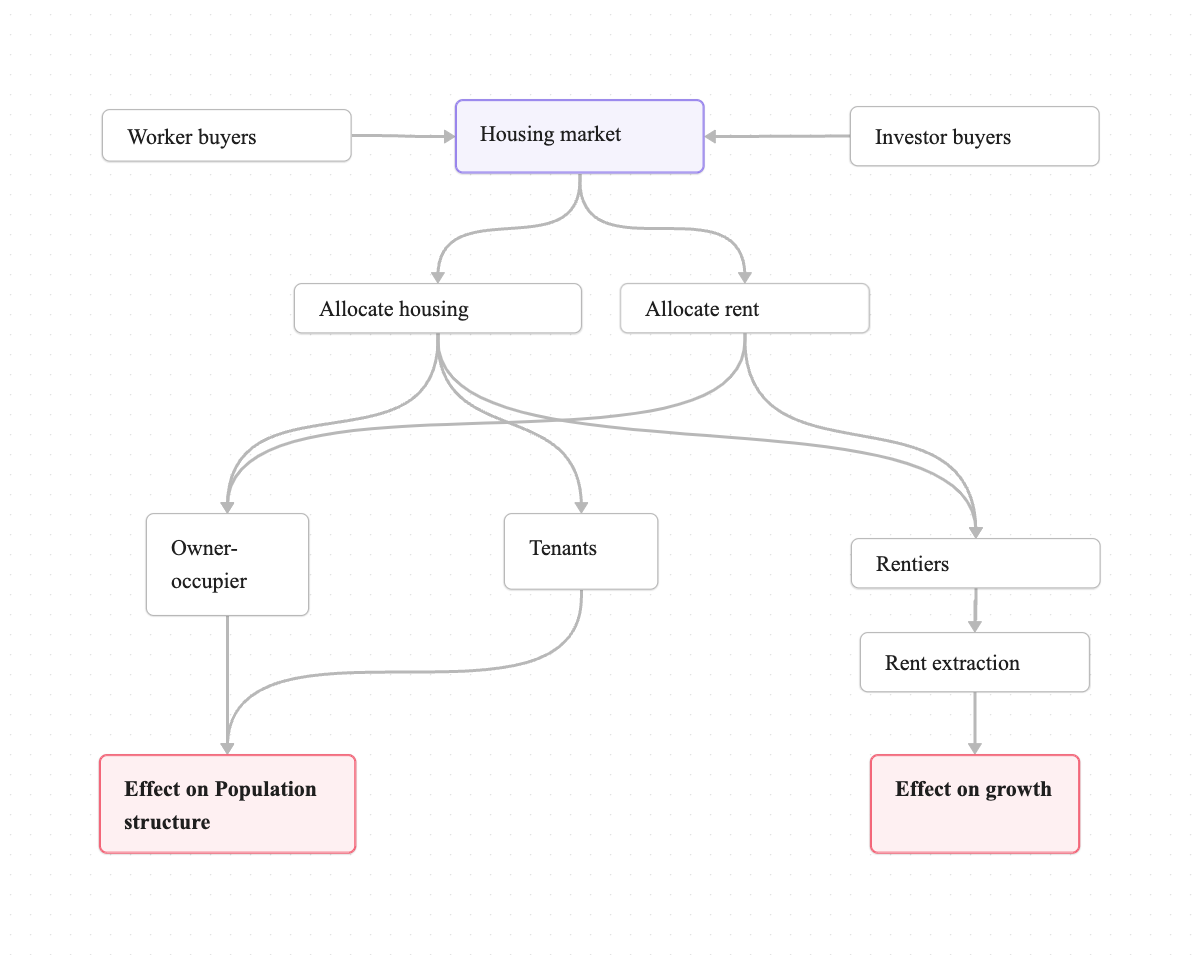
\includegraphics[scale=.60]{fig/flow_impacts.png}
    \label{Figure-impacts}
\caption{Impacts.}
\end{figure}



***
One of the founding questions economics emerged to explore is how wealth is distributed across different groups or classes. Property ownership is one of central ways for building wealth throughout history. Widely distributed property home ownership has contributed to the wide distribution of welath particularly in North America. It is a key differentiator between who has gotten build wealth and who hasn't. %This is seen in the racial wealth gap, the immigrant wealth gap, and the youth wealth gap. 

MORE IS OWNED BY FINANCIAL....

Because of this sigificance of propoerty to welkth disribution financial has big effect for distribution. This is accept SEEN IN XY say. 

This thesis says it also has dramatic effects for productivity of cities.....
There's now compelling understanding of the value that's created by urban systems, empirically and theoretically, but there's no formal apparatus, in standard economic theory,  for understanding/analyzing the distribution of that enormous value that's being created.

The idea of financialization of the housing market has been gaining currency. ***E IN WHAT SENSE? %SAY WHAT IT IS GAINING CURRENCY FOR... AMOUNG WHAT GROUP TO EXPLAIN WHAT... THE HOUSING CRISIS? THEN EXPLIAN BUT IT'S HAS DEEPER/MORE SIGNIFICANT EFFECTS ON SYSTEMS....
 
This dissertation makes the case that it has worrying implications for the success of cities and the nature of our social fabric. 

 % ***E I THINK THE FOLLOWING PARAGRAPH SHOULD BE REPHRASED SLIGHTLY TO FIT THIS LOCATION BETTER. % ***E i COULD DO THIS LATER.... i THINK THAT IT IS NOT NECESSARY TO SAY ALL THE MEANINGS OF THE WORD HERE, JUST SAY WHAT YOU ARE LOOKING AT IN THIS THESIS, "
 
 While the term financialization can be used in a variety of ways, the macro effects of financialization are the specific concern of this thesis.  Financialization, in this sense, refers to %how financialized markets.... 
 % The term financialization is used in a variety of ways:  for developing legal instruments that facilitate financial transaction;  
 the growth in the share of the housing stock controlled by financial institutions and investors and the overall effect this has on the outcomes of system. These macro effects are our main interest. 

We develop a model which suggests two basic results/hypotheses:
\begin{enumerate}
    \item Financialization of the housing market will result in the decline of the urban middle class and
    \item Financialization of the housing market will result in reduced growth of urban productivity.
\end{enumerate}

% ***e wHAT FOLLOWS GOES INTO DETAIL TOO QUICKLY. IT'S HARD TO KEEP UP. MAYBE THIS IS A PLACE TO 
ADD A BIT MORE CONTEXT ABOUT WHAT THE PROBLEM IS THAT THE METHODS IN THIS THESIS ARE TRYING TO FIX

The housing market allocates both the housing stock and the land \glspl{rent} generated by the urban system as illustrated in Figure\ref{Figure-impacts}. Our argument is that the first effect arises because the rents generated by the agglomeration economies in the urban system are diverted to largely non-resident owners and away from investment in local production or amenities. 
% VS - SPEND TO PRODUCE - WE DO SOMETHING MORE NARROW?

The second effect arises because, with growing financialization of the housing market, owner-occupiers are gradually replaced by tenants.  Owner-occupiers share in the growing land rents generated by urban agglomeration effects, tenants do not. As a result, a declining fraction of urban residents accumulate capital through their participation in the housing market, and therefore fewer enter the class with both wage and capital income. 

\begin{figure}[!ht]
    \centering
    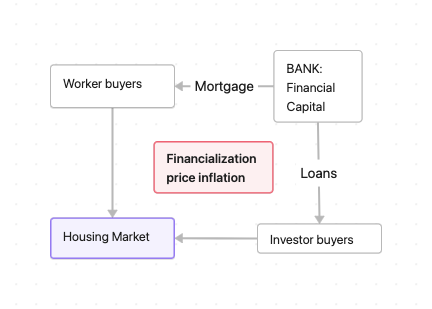
\includegraphics[scale=.70]{fig/flow_financialization.png}
    \label{Fig-financial-cycle}
    \caption{Financial capital}
\end{figure}



Figure~\ref{Figure-impacts} shows the main effects  that  arise from the growing financial sector participation in the housing market. Behind the market process are two sub-models. The first, illustrated in Figure\ref{Fig-financial-cycle}  develops an explicit model of investor behaviour to explain the market decisions of buyers and the role of financial capital. This is discussed in detail in Chapter~\ref{chapter-financialization}.

The key observation is that investors enter the housing market. In doing so they drive up prices by increasing total demand. The rising price generates an expectation of capital gains, which enters the investors' calculations. Investors have, as research shows, better access to capital than most new entrants to the housing market. When the financial sector, represented by the Bank in Figure\ref{Fig-financial-cycle}, makes more capital available, the pattern of ownership shifts, as illustrated above.

\begin{figure}[!ht]
    \centering
    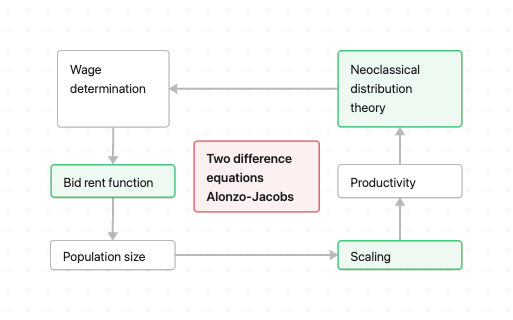
\includegraphics[scale=.7]{fig/flow_Alonzo-Jacobs_cycle.png}
    \label{Fig-Alonzo-jJacobs-cycle}
\caption{The Alonzo-Jacobs cycle.}
\end{figure}

The second sub-model incorporates  productivity of cities. Geoffrey West has argued that ``Cities are the crucible of civilization, the hubs of innovation, the engines of wealth creation and centers of power, the magnets that attract creative individuals, and the stimulant for ideas, growth, and innovation.'' \cite{westScaleUniversalLaws2017} CHECK SOURCE. This is of course a theoretical argument associated with the work of Jane Jacobs \cite{jacobsEconomyCities1969}, although has strong theoretical and empirical support  \cite{bettencourtGrowthInnovationScaling2007, bettencourtOriginsScalingCities2013, dongUnderstandingMesoscopicScaling2020, loboUrbanScalingProduction2013} that we discuss in Chapter~\ref{chapter-rent}. In that chapter we ground the observation in  \gls{neoclassical growth theory} and recent empirical and theoretical work on \gls{urban scaling}. We then  incorporate that result into the standard urban model,  associated with William Alonzo \cite{alonzoTheoryUrbanLand1960}.   We describe The Alonzo model in Chapter~\ref{chapter-space}. We call the combined sub-model the \gls{Alonzo-Jacobs model}.   

***E THIS SUMMARY OF WHAT YOU MODEL IS GOOD. IT MOVES A BIT FAST AND THERE COULD BE MORE CONTEXT, 

When these components are  combined,  we have an extended theory of urban rent built on a foundation of theory that goes back to the \gls{classical economics} around the beginning of the 19$^{th}$ century and incorporating modern growth theory and modern urban theory.

% SOMEWHERE IN THIS INTRODUCTION SAY THIS THESIS IS MODERN URBAN RENT THEORY. 

 % MOVE THIS TO SPACE?
%Missing- transfer of money vs put in a spatial framework.
%Most of the economic theory talks about where people go, and it doesn't talk about the value they create in the city and where that goes. That's finacialization, capturing those benefits is what capitalists are doing now.
% rent is being in the house/what they pay, the transfer of money, vs what cities are, and how that produces value..

% Canada faces a housing crisis. The crisis now reaches far into the middle class, causing everything from declining home ownership rates to increasing poverty and displacement. 
%In the last few years, the need for affordable housing has come into focus as one of the most pressing issues facing Canadians. % ***E (ADD STRIKING STATISTIC - A NUMBER OR QUOTATION HERE.) 
% As more and more Canadians are finding 
%As more Canadians find housing unaffordable, the effects 
 % number of Canadians able to afford housing at all, leading to vacancies, poverty, and displaced workers. % (***E FILL THIS OUT A BIT - ADD SOME DETAILS HERE ABOUT THE EFFECTS OF THE CRISIS - THAT SET UP THE RESULTS OF THE THESIS)
% RATE OF INCREASE -VITAL SIGNS REPORT, CMHC
% There has been extensive debate about the drivers of the crisis. ADD FACTS. Proposed explanations include supply shortages, stagnating incomes, and the financialization of housing ownership. 
% (Centering on two dominant stories, a story of supply and demand and one of rights.) %FIX and cite

% There has been less work on the implications for productivity. 
% In this thesis we focus on the financialization of housing ownership and its impact on urban productivity in an economy driven by urban agglomeration effects. 

% The source of the rents captured and the broader social and economic effects have not been fully captured. 
 % This provides insight into both population and wealth distribution in cities. 
% Integrating financial markets into the the spatial urban model allows us to examine the effect of financialization on cities, specificaly on their role in growth, distribution, and productivity. % the growth and wealth distribution of cities, and more specifically on their productivity effects. 

MOVE THIS UP?
Our approach draws together insights from % economics and the study of cities. 
% Our model of the urban economy is based on work from those developed in 
geography, planning and urban economics. 
The organizing principle in the spatial models of all three disciplines is an economic variable, land rent, which is for us the link to distribution, financialization and continuing productivity. %*** (another sentence on why this is great) --The space-less quality of the study of finance leaves out xyz GET PHRASING- CAN'T SEE- INTEGRATION OF SPACE NEGLECT GROWTH FACTOR. 

Rent is important is all these traditions, but has been neglected in modern theory. We argue that to formally understand the processes behind financialization and the housing crisis, what's needed is a modern urban theory of rent. This thesis is a contribution to the development of that theory.

% BUT THERE ARE OTHER THINGS MISSING - NO RENT, NO SPACE IN FINANCE, PRODUCTIVITY NOT RELATED TO SPACE OR LOCATION.

To capture urban productivity, we introduce %rely on 
agglomeration effects, relating existing spatial and growth models to the scaling models from the study of complexity. A fundamental feature in recent empirical work on scaling laws is % demonstrated in the recent literature on scaling laws: 
the persistent relationship between population and productivity. The productivity of cities increases superlinearly with population. Cities are the locus of a positive feedback loop with rising populations raising productivity, and rising productivity attracting more people and resource.


% Thus The productivity implications of the housing crisis are the focus of this thesis.

%(***E DEFINE TO SET UP THE DISTRIBUTIVE FEATURES OF ECONOMY). 
 % ***E ADD: the effects of housing affordability are pervasive / complex /run through the whole system / go far behind the obvious /direct effects / extend in non-obvious ways through the economy/whole system. What is at stake at a broader level is. 
% Yet, the economics is clear that what's at stake is the productivity of cities, the distributive features of the economy and the impact of the middle class % THIS IS A RESULT NOT AN INPUT. WHAT GOES HERE? ***E MAYBE ADD A CLARFIYING CONCLUDING SENTENCE HERE.... TO SAY SOMETHING LIKE THE EFFECTS OF HOUSING PRICES ARE NOT LIMITED TO 

% SAVE THIS ?? The greatest price increases have been in cities, where where people live and work, where  production is concentrated and where income is distributed. With humans becoming an increasingly an urban species, cities are a primary driver of technological development and increasing wealth. 

% (TIE BACK TO HOUSING CRISIS - EG. The affordability 
% \textbf{HOW WE ADD IT BACK IN}
%This thesis presents a spatial model of the city that incorporates distributional issues and financialization and allows us to examine the productivity implications of the housing crisis. The model that incorporates the scaling of productivity in cities within a standard urban model. 


%\textbf{WHY IT'S BEEN MISSING} EXPLAIN BETTER HERE WHY SPACE HAS BEEN LEFT OUT, AND WHY THAT LET'S US NEGLECTS SPATIAL RENTS AND MISS THE RELATION BETWEEN SPACE AND PRODUCTIVITY.
% We see urbanization and continuing and financialization accelerating. Financialization is driven by capital seeking profits, but what is the source of the rents they capture? The answer is in conventional urban theory, which allows us to identify the spatial distribution of those rents and traditional rent theory, which allows us to understand the social relations of those, those rents, the classical economists spend a great deal of time on that question. And we're very clear about it.
%We're talking about what is the puzzle? This is the teaser for this thesis and this thesis offers an answer to and I've just started to suggest that the teaser is given that 

% fig
% ***E I THINK THE PARAGRAPH ABOVE IS SAYING:  
% While financialization is usually understood as capital seeking prxfit, the source of the rents captured and the broader social and economic effects have not been fully captured.  XXXZ The current models for understanding financialization and it's effects don't predict the actual trends we are see. {\color{red} We argue this is because they miss the importance of space FIX.} 

%COMPELLING DESCRIPTION OF WHAT'S MISSING IN THE LITERATURE
%these share space, formalization in finance is spaceless

The housing crisis raises the question of whether Canadian cities can continue to attract people and accumulate wealth for its residents and industries, and whether they can sustain their growth.
% Our focus is land rents, %but in the context of an urban economy. 

Integrating classical and neoclassical economic approaches with traditional urban theory,  allows us to identify 
 we can build a more comprehensive model of financialization and its effects. This makes it possible to trace the spatial distribution of the rents.

This thesis  is thus a contribution to developing a modern theory of urban rents.

LINK/MOVE?
While financialization is usually understood as capital seeking profit, in the urban context it is a fundamentally spatial phenomenon. %also a spatial  phenomenon. 
***E MAYBE MOVE THIS UP... IT MIGHT BE HELPFUL CONTEXT FOR WHAT YOU ACTUALLY DO, IT BEGINS TO ESTABLISH THE PROBLEM
Its goal is the capture of spatial rents, which, we will show, has implications for both the productivity and the class structure of the city. These aspects of finacialization in the urban system have been neglected in the literature. Standard models of the financial operations are spaceless.\footnote{In describing any theory we need to identify the kinds of objects that are theorized. Financial analysis theorizes  assets, debts, flows of revenue and costs, and the rates of change or exchange of these quantities over time. These are inherently spaceless because they are accounting entities, completely independent of location. It matters where a worker or a farm is. It does not matter where and dollar or a rouble is.} 
Our solution is to explicitly link the largely spaceless analysis of investment decisions to spatial rents in an urban system. 

%The effects of financialization on cities and economies has not been fully accounted for because the tools of the different, relevant disciplines have not been adequately integrated. The current approaches to describing the financialization of housing and its effects predict / explain /account for the housing crisis and effects on home ownership and access to housing, but our work shows that there are broader effects that have not been accounted for / predicted. 


% This fuller picture is made possible by bringing together classical rent theory, neo-classical XX and urban theory to create/and using/along with a agent-based model that allows us to .... (What the modelling technique enables) 

% \textbf{WHICH GIVES US THESE CONTRIBUTIONS}
% \section{Contributions}
%PROBABLY INTEGRATE WITH THE ABOVE, MAYBE MAP/HIGHLIGHT CONTRIBUTIONS IN A FIGURE/TABLE

%This work is important for understanding the current policy context. 
The analysis makes clear that in addition to the recognized distributional consequences, the housing crisis has productivity impacts that should be considered in developing urban and housing policy. Particularly, it centers concern with implication for urban development of growing rent extraction by the financial sector. 

\section{Position in the literature}
How does this fit in the larger literature?

The focus of this thesis is a topic that falls in the overlap between three academic  disciplines, Economics, Urban Geography, and Planning. % ***E mAYBE SUMMARIZE THE FOCUS OF EACH? While Economics traditionally focuses on... Urban Geography looks at ..... and Planning is the study of....
The central and shared concern in this area is with geographic space. % ***E DO YOU MEAN GEOGRAPHIC SPACE AND PEOPLE SOMEHOW? i FEEL LIKE YOU DON'T MEAN THIS? MAYBE MORE LIKE: The central shared concern between the three discipline it the role of geographic space in shaping WHAT? social and economic systems? human systems? society??
% \begin{figure}
% \begin{tikzpicture}{scale=.5}
% % find color cotrol for ball. Tind way to stop line short of node
% \coordinate (planning) at (-5,1);%PREFACE
% \coordinate (economics) at (5,.75);%
%  \coordinate (geography) at (-.5,-2); %history
% \coordinate (finance) at (0,5); %

% \draw [line width=2mm, black!15, ] (planning)--(economics);
% \draw [line width=2mm, black!20, ] (geography)--(economics);
% \draw [line width=2mm, black!20, ] (geography)--(planning);

% %\draw [line width=2mm, black!25, ] (geography)--(finance);
% %\draw [line width=2mm, black!20, ] (planning)--(finance);
% %\draw [line width=2mm, black!20, ] (finance)--(economics);
% \node [circle,shading=ball, minimum width=2.1   cm, white, align=center] (ball) at (planning) {Planning};
% \node [circle,shading=ball, minimum width=2.2cm, white, align=center] (ball) at (economics) {Economics};
% \node [circle,shading=ball, minimum width=3cm, white, align=center] (ball) at (geography)[text width=2cm] {\large Urban\\ Geography};
% %\node [circle, shading=ball, minimum width=2.4cm, white, align=center] (ball) at (finance)[text width=2cm] {Finance};

% \node at (-.3,-.1) [red] {\Large \textbf{Space}};
% \end{tikzpicture}
% \caption{The common concern of three fields topic }
%     \label{fig-three-fields}
% \end{figure}
The three disciplines share a simple economic insight in all three area: that locational value gives rise to land rents.  % CUT the three disciplines where they overlap. 
% ***E REPLACE WITH: 
Locational value explains the spatial distribution of human activities, urban form,  % because EXPLAIN.  % DEFINE... 
and the dynamics of economic development.  Our focus, however is on who captures these rents and how that affects the city. The distribution of locational rents, we believe, goes some distance to explaining core social issues like class structure, inequality, political political power %ADD SUMMARIZING SENTENCE

%***E ADD:This thesis describes a model that draws together LIST HERE. 
. % ***E OR list all??? ie. From Classical Rent to Neo-Classical Marginalist theory to XYZ urban theory and ...... etc. SET UP THE WHOLE SECTION.
%E ADD: The concept of rent illustrates WHAT in relation ot distribution, allows what kinds fo insights, which sets up this work.  We use the concept of rent to frame our consideration of how wealth is distributed in society by looking at WHAT?? how surplus is distributed? how locational value and location OR WHAT?? affects surplus distribution?? I dont know but please summarize how rent is used in this thesis. 

Nearly contemporaneous thinker, Johann Heinrich  von Th\"unen (1783-1850) developed a planning model to guide the location of economic activities for an urban-agricultural society.  A version of that model  was reinvented in urban geography by XXX. Alonzo\footnote{We use a version of the well-established model of Alonso (1964), Muth (1969) and Mills (1967), and formalised by Wheaton (1974),} % ***E NEED MORE DETAIL HERE ABOUT ALONZO"S MODEL, 

We link the Alonzo model with more recent work on growth theory starting with Robert Solo's XXX and with the endogenous growth models of Lucas () and draw on Jane Jacobs's insight that endogenous urban growth  is. now driving economic development. Jacobs's insight is empirically supported by recent work in the complexity literature on urban scaling by XXXX ()



\begin{figure}
    \centering
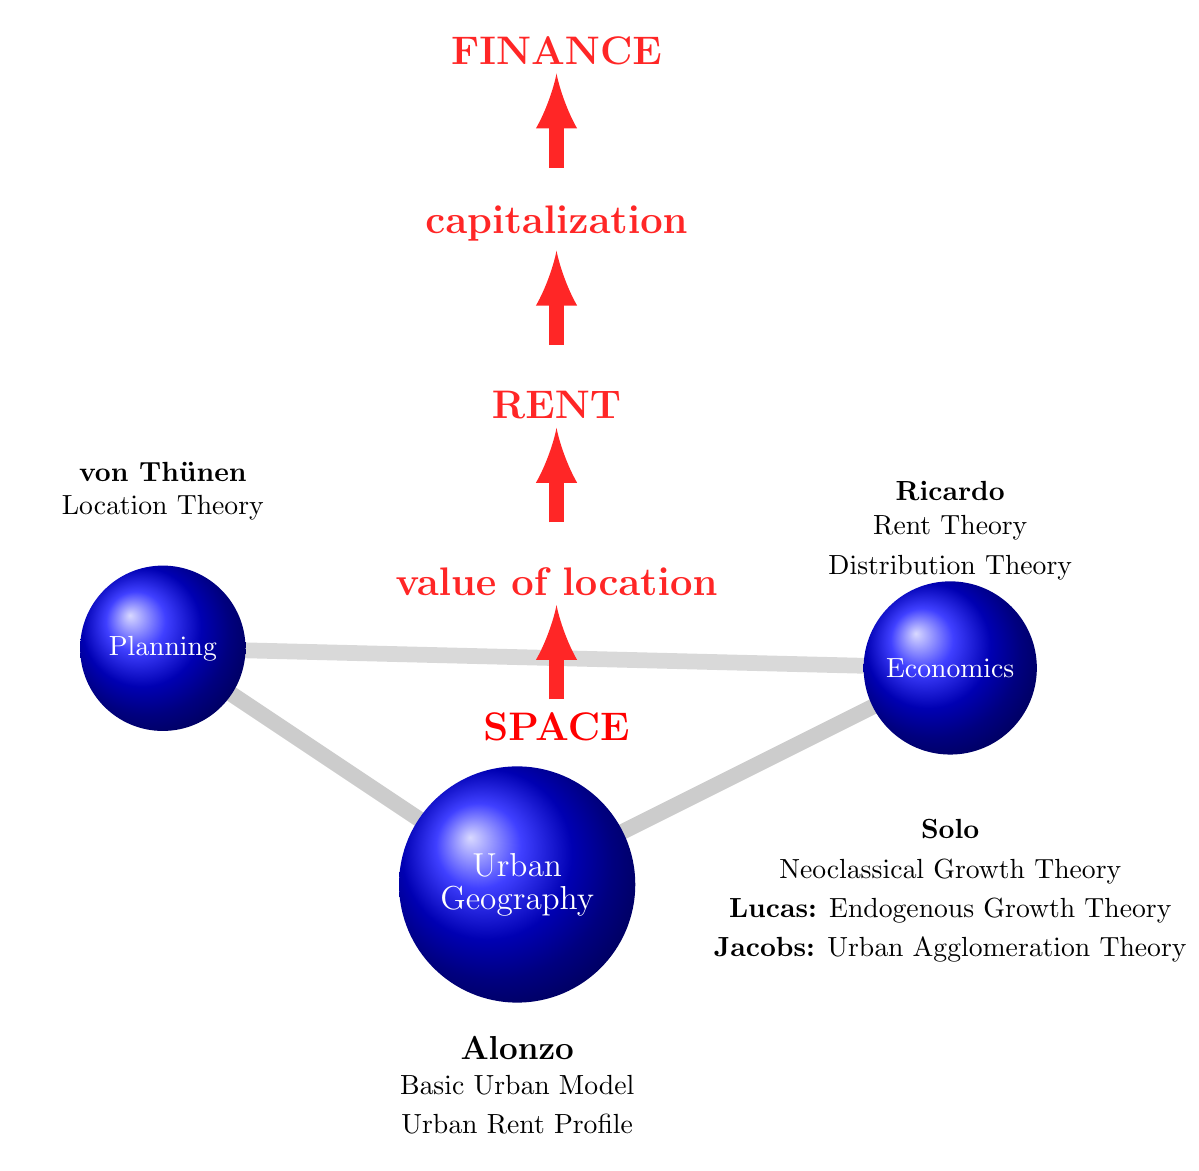
\begin{tikzpicture}{scale=.5}
% find color cotrol for ball. Tind way to stop line short of node
\coordinate (planning) at (-5,1);%PREFACE
\coordinate (economics) at (5,.75);%
 \coordinate (geography) at (-.5,-2); %history
\coordinate (finance) at (0,5); %

\draw [line width=2mm, black!15, ] (planning)--(economics);
\draw [line width=2mm, black!20, ] (geography)--(economics);
\draw [line width=2mm, black!20, ] (geography)--(planning);

%\draw [line width=2mm, black!25, ] (geography)--(finance);
%\draw [line width=2mm, black!20, ] (planning)--(finance);
%\draw [line width=2mm, black!20, ] (finance)--(economics);

\node [circle,shading=ball, minimum width=2.1   cm, white, align=center] (ball) at (planning) {Planning};
\node [circle,shading=ball, minimum width=2.2cm, white, align=center] (ball) at (economics) {Economics};
\node [circle,shading=ball, minimum width=3cm, white, align=center] (ball) at (geography)[text width=2cm] {\large Urban\\ Geography};

%\node [circle, shading=ball, minimum width=2.4cm, white, align=center] (ball) at (finance)[text width=2cm] {Finance};

%\node at (-.3,-.1) [red] {\Large \textbf{RENT}};

% new stuff
\node at (planning) [above=2cm] {\textbf{von Th\"unen}};
\node at (planning) [above=1.5cm] {Location Theory};

\node at (economics) [above=2cm] {\textbf{Ricardo}};
\node at (economics) [above=1.5cm] {Rent Theory};
\node at (economics) [above=1.0cm] {Distribution Theory};

\node at (economics) [below=1.8cm] {\textbf{Solo}};
\node at (economics) [below=2.3cm] {Neoclassical Growth Theory};
\node at (economics) [below=2.8cm] {\textbf{Lucas:} Endogenous Growth Theory};
\node at (economics) [below=3.3cm] {\textbf{Jacobs:} Urban Agglomeration Theory};


\node at (geography) [below=1.8cm] {\textbf{\large Alonzo}};
\node at (geography) [below=2.3cm] {Basic Urban Model};
\node at (geography) [below=2.8cm] {Urban Rent Profile};

%\node [circle, shading=ball, minimum width=2.4cm, white, align=center] (ball) at (finance)[text width=2cm] {Finance};
\draw [line width=2mm, red!85, -latex ] (0, 7.1)--++(0,1.2)node[above=-.1] {\Large \textbf{FINANCE}};
\draw [line width=2mm, red!85, -latex ] (0, 4.85)--++(0,1.2)node[above=-.1] {\Large \textbf{capitalization}};
\draw [line width=2mm, red!85, -latex ] (0, 2.6)--++(0,1.2)node[above=-.1] {\Large \textbf{RENT}};
\draw [line width=2mm, red!85, -latex ] (0, .35)--++(0,1.2)node[above=-.1] {\Large \textbf{value of location}};
\node at (0,0) [red] {\Large \textbf{SPACE}};


\end{tikzpicture}

    \caption{space and value ***TODO FLIP ECON AND PLANNING TO FOLLOW ORDER OF CHAPTERS}
    \label{fig-space-value}
\end{figure}

Land rent was historically the basis of the wealth and political power of  the land-owning class in the era of the classical economists. % ***E NEED MORE HERE


We further link the model of urban rents to emerging concerns about the financialization of the housing market. The key insight we offer is that the financialization  of the housing sector is a  form of rent-seeking that must have detrimental effects on urban development and on the well-being of urban residents.


% ***E NEED TO POSITION THIS WORK IN RELATION TO THE MARGINALIST ACCOUNT IN THIS SECTION BECAUSE IT IS ONE OF THE FEW THINGS YOU HAVE INTRODUCES. tHE URBAN MODELS YOU DESCRIBE HERE SHOULD BE FRAMED BY WHAT YOU ADD IN BACKGROUND ABOUT PLANNING/URBAN MODELS (AS PER MY SUGGESTION IN THAT SECTION) 
% ***E YOU ALSO NEED TO ADD A SUMMARIZING PARAGRAPH WHICH I CAN HELP WRITE WHEN THIS SECTION IS MORE FILLED OUT. MAYBE THIS:
% ***E ADD: By bringing these approaches into a coherent approach, we can better account for  WHAT... EXPLAIN THAT alone they don't give as complete a picture. This thesis show that certain things become clear when they are brought together that provide an better account of the current situation. Older economics models do not predict certain things that are currently happening. This is because they are based on out of date modes of production, fail to account for the importance of location value and the modelling tools available when they were developed required some simplification.   Updating the models for the changing times, using more complex modelling systems and incorporating space with the economic models allow us to create models and narratives that provide a more effective understanding of the situation as it stands today. 





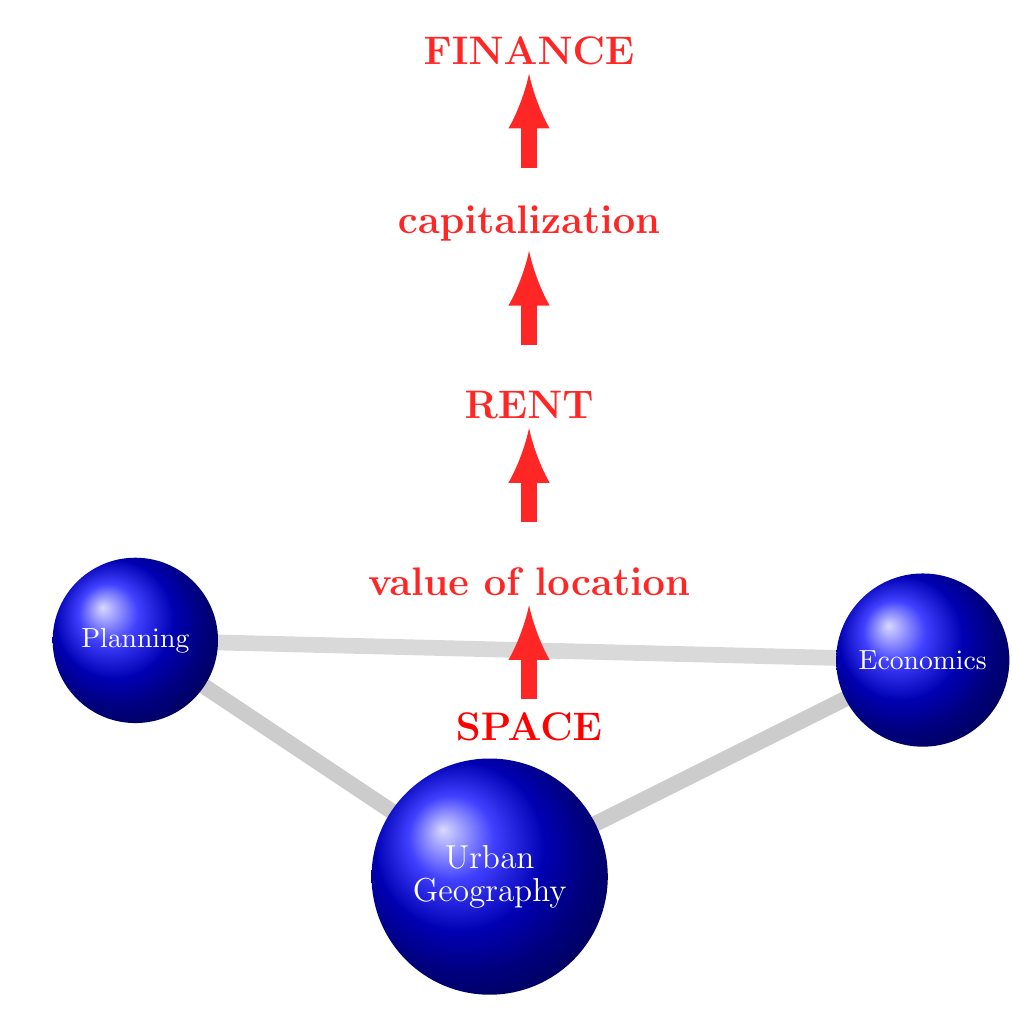
\begin{tikzpicture}{scale=.5}
% find color cotrol for ball. Tind way to stop line short of node
\coordinate (planning) at (-5,1);%PREFACE
\coordinate (economics) at (5,.75);%
 \coordinate (geography) at (-.5,-2); %history
\coordinate (finance) at (0,5); %

\draw [line width=2mm, black!15, ] (planning)--(economics);
\draw [line width=2mm, black!20, ] (geography)--(economics);
\draw [line width=2mm, black!20, ] (geography)--(planning);

%\draw [line width=2mm, black!25, ] (geography)--(finance);
%\draw [line width=2mm, black!20, ] (planning)--(finance);
%\draw [line width=2mm, black!20, ] (finance)--(economics);

\node [circle,shading=ball, minimum width=2.1   cm, white, align=center] (ball) at (planning) {Planning};
\node [circle,shading=ball, minimum width=2.2cm, white, align=center] (ball) at (economics) {Economics};
\node [circle,shading=ball, minimum width=3cm, white, align=center] (ball) at (geography)[text width=2cm] {\large Urban\\ Geography};

%\node [circle, shading=ball, minimum width=2.4cm, white, align=center] (ball) at (finance)[text width=2cm] {Finance};
\draw [line width=2mm, red!85, -latex ] (0, 7)--++(0,1.2)node[above=-.1] {\Large \textbf{FINANCE}};
\draw [line width=2mm, red!85, -latex ] (0, 4.75)--++(0,1.2)node[above=-.1] {\Large \textbf{capitalization}};
\draw [line width=2mm, red!85, -latex ] (0, 2.5)--++(0,1.2)node[above=-.1] {\Large \textbf{RENT}};
\draw [line width=2mm, red!85, -latex ] (0, .25)--++(0,1.2)node[above=-.1] {\Large \textbf{value of location}};
\node at (0,-.1) [red] {\Large \textbf{SPACE}};
\end{tikzpicture}



% \vspace {2cm}
% Figure 4 with finance

% \begin{tikzpicture}{scale=.5}
% % find color cotrol for ball. Tind way to stop line short of node
% \coordinate (planning) at (-5,1);%PREFACE
% \coordinate (economics) at (5,.75);%
%  \coordinate (geography) at (-.5,-2); %history
% \coordinate (finance) at (0,5); %

% \draw [line width=2mm, black!15, ] (planning)--(economics);
% \draw [line width=2mm, black!20, ] (geography)--(economics);
% \draw [line width=2mm, black!20, ] (geography)--(planning);

% \node at (-.3,2) [red] {\huge \textbf{RENT}};

% \draw [line width=3mm,  black!50,opacity=.5 ] (geography)--(finance);
% \draw [line width=2mm, black!20, ] (planning)--(finance);
% \draw [line width=2mm, black!20, ] (finance)--(economics);

% \node [circle,shading=ball, minimum width=2.1   cm, white, align=center] (ball) at (planning) {Planning};
% \node [circle,shading=ball, minimum width=2.2cm, white, align=center] (ball) at (economics) {Economics};
% \node [circle,shading=ball, minimum width=3 . cm, white, align=center] (ball) at (geography)[text width=2cm] {\large Urban\\ Geography};

% \node [circle, shading=ball, minimum width=2.4cm, white, align=center] (ball) at (finance)[text width=2cm] {Finance};


% \end{tikzpicture}



\vspace {2cm}
Figure 4 with finance

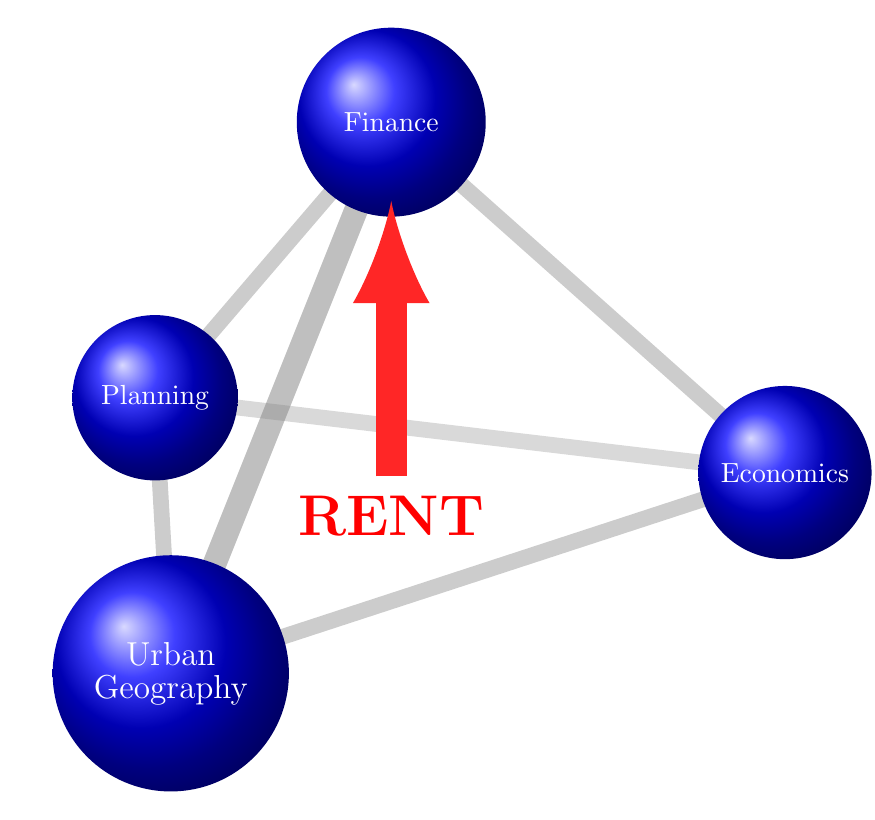
\begin{tikzpicture}{scale=.5}
% find color cotrol for ball. Tind way to stop line short of node
\coordinate (planning) at (-3,1.5);%PREFACE
\coordinate (economics) at (5,.55);%
 \coordinate (geography) at (-2.8,-2); %history
\coordinate (finance) at (0,5); %

\draw [line width=2mm, black!15, ] (planning)--(economics);
\draw [line width=2mm, black!20, ] (geography)--(economics);
\draw [line width=2mm, black!20, ] (geography)--(planning);

\node at (.0,0) [red] {\huge \textbf{RENT}};

\draw [line width=3mm,  black!50,opacity=.5 ] (geography)--(finance);
\draw [line width=2mm, black!20, ] (planning)--(finance);
\draw [line width=2mm, black!20, ] (finance)--(economics);

\node [circle,shading=ball, minimum width=2.1   cm, white, align=center] (ball) at (planning) {Planning};
\node [circle,shading=ball, minimum width=2.2cm, white, align=center] (ball) at (economics) {Economics};
\node [circle,shading=ball, minimum width=3cm, white, align=center] (ball) at (geography)[text width=2cm] {\large Urban\\ Geography};

\node [circle, shading=ball, minimum width=2.4cm, white, align=center] (ball) at (finance)[text width=2cm] {Finance};
\draw [line width=4mm, red!85, -latex ] (0, .5)--(0,4);
\end{tikzpicture}

\section{Contributions}
The main contributions, % methodological innovations
as we see it, are ROUGH LIST. TO SUMMARIZE AND SORT:

% \begin{enumerate}
%     \item we incorporate \gls{classical rent theory} into an agent-based urban model 
%     \item we allow the creation and distribution of rents to influence urban growth, productivity and  population structure. 
%     \item we incorporate current research on \gls{urban scaling} into the  core spatial urban model.   
%     \item we construct an   Urban \gls{ABM} that is consistent with \gls{neoclassical growth theory},
%     \item we integrate \gls{financial capital} into a standard spatial model of the urban system
%     \item we integrate financial capital into an population model of the urban system
%     \item we employ the ABM to examine how financial markets impact the urban land markets 
%     \item we test for \gls{hysteresis}  resulting from the business cycle  in the urban system 
%     \item we build a model that is easily extended to explore a wide range of issues
%     \item we provide a model that we believe can be used  to evaluate urban policies
% \end{enumerate}

Each of the items above requires us to  integrate models and concepts from different parts of the literature. 

ADD TO EACH: THIS MEANS, THIS MATTERS BECAUSE, THEN FOLLOW WITH TO DO IT, WE NEED TO.

% CONSIDER MENTIONING WHAT ORDER THIS IS IN  % It's a kind of logical order, almost in the order of development: (types, order implemented, order theory is developed, order of importance?)

IS THERE A PICTURE THAT COULD ILLUSTRATE THE CONTRIBUTIONS?

\begin{enumerate}
    \item incorporating \gls{classical rent theory} into an agent-based urban model 

This requires a how Ricardian rent theory - a theory of distribution based on an agricultural economy - applies in an economy driven by human capital agglomeration effects within the urban system. 

    \item allowing the creation and distribution of rents to influence urban growth, productivity and  population structure. 
    
This requires us to articulate the links between the wealth production of cities and  urban systems evolve 

    \item incorporating current research on \gls{urban scaling} into the  core spatial urban model.  

We show how understanding how complex systems scale provides an elegant way to model a an urban system with production

    \item constructing an urban \gls{agent-based model} that is consistent with {neoclassical growth theory},

% Although many  who employ ABMs to analyse urban systems are deeply skeptical of neoclassical assumptions
We demonstrate in this context how %easily and productively 
the neoclassical framework can be implemented in the agent-based framework, and make a case for it's usefulness in linking urban rents and productivity, linking traditions that have been seperate. 

In general, there is relatively little work rigorously linking analytic and agent based models, so the results can be understood formally, in relation. % incorporated into prior traditions and

    \item integrating \gls{financial capital} into a standard spatial model of the urban system

% We are not aware of any urban simulation models that
We introduce capital within this framework in a novel way. %as we do to examine the outcomes that concern us.
    
    \item integrating financial capital into an \gls{overlapping generations} population model of the urban system

Financial assets are central to most overlapping generations models. Our innovation is to articulate the movement of financial capital though the urban land market. 

SOMETHING LIKE Adding space to finance which has been spaceless.
    
    \item using an ABM to examine how financial markets impact  urban \glspl{land market}.

We began with with the fact that there is growing policy concern about the ``Financialization of  Housing''. We have produced a formal simulation model that illustrates the process. 

    \item testing for \gls{hysteresis} resulting from the business cycle   in the urban system, exploring the \gls{resilience} implication's of the core spatial economic model

There are two types of resilience questions when any system is shocked, does it return to an https://www.overleaf.com/project/606a6b286ae1c9f203fadab5equilibrium state - the stability question - and does it return to the same kind of equilibrium - the hysteresis question. We focus on the latter question.  

    \item building a model that is easily extended to explore a wide range of issues

The model combines clear and explicit theoretical assumptions with careful and transparent implementation of the logic in flexible Python code.

    \item providing a model that we believe can be used  to evaluate urban policies

To be useful in policy discussions, a model must correctly simulate the relevant system features and be able to incorporate a variety of policy interventions. We have taken care to allow for  both theoretical and policy- relevant extensions in the way the simulation model is coded. 
\end{enumerate}

(** ``The notion that your labour force is on average more productive when there are more people around is pretty dramatic and it's very much not part of the basic model that we use. Our starting point is that's the fundamental feature of cities, and what does that do with financial capital and what does that do to distribution and that's not been explored. PUT THIS IDEA HERE?)

\section{Document overview}
This thesis develops a conceptual framework for a model of the housing market and then describes the model and the implications of the analysis of the model. %insights it produces. 
There are three parts in the dissertation. 

MAYBE LINK ORDER TO POSITION IN THE LIT/CONTRIBTUIONS AGAIN % 3 PARTS TO THE MODEL, DEVELOPMENT FOLLOWS THE TRAJECTORY OF THIS. 

Part \ref{part-background} gives the background and introduces the theoretical framework for the analysis,  linking classical rent theory, neoclassical production theory, neoclassical growth theory, the scaling literature, and urban spatial models. 

\begin{enumerate}
    \item Chapter \ref{chapter-background} sketches how this thesis relates to four major fields: classical rent theory, neoclassical production theory and growth theory, the scaling literature, and urban spatial models. %..., and the role of space as a unifying factor across three of the fields. % WITH FINANCE IS SPACELESS.
    % *** ADD BACK? This work draws together sub-literatures including rent theory, production functions, the standard urban model, growth theory, urban growth theories, financialization, and the theory of distribution, so the chapters review those areas. % *** link the areas to the chapters better?  %theory for our analysis, 
    \item Chapter \ref{chapter-rent} reviews the literature on rent and develop an approach suited to the analysis for this work.
    \item Chapter \ref{chapter-growth} introduces growth theory, showing how our model is directly connected with this broad collection of linked theories. %, we use the Cobb-Douglas function, which is used across this entire range of literature - frame the relation of a tradition in context of  % After we develop the mathematical description of the relationship among these will discuss  in more detail, rent theory and our contribution, scaling laws, ......  and other issues in the literature that draw on parts of this model and % ???  apply to the specific situation we're in why rent theory is related to discussions of exploitation why it might lead the inefficiencies, whether or not this links with other important models in the literature.
    \item Chapter \ref{chapter-space} develops the urban model of space drawing on the basic Alonzo model.
    \item Finally Chapter \ref{chapter-financialization} provides a description of finacialization, and explores the potential consequences of fiancialization in the housing market.  % showing it is a form of rent-seeking in the housing market and ?? 
\end{enumerate}
 
Part \ref{part-model} develops the model and results.
\begin{enumerate}
    \item Chapter \ref{chapter-methodology} introduces the methodology. % In addition to the core contribution linking housing and productivity, there are three methodological lines of contribution, and there are policy implications SUMMARIZE METHODOLOGICAL CONTRIBUTIONS %(rent is key to financialization, however the main urban models don't observe the distribution of rents)
    \item Chapter \ref{chapter-model} describes an illustrative agent-based model of the urban system. 
    This model has three  parts, first a production function, modelling how urban regions generate wealth, and second a model of an urban housing market, and finally, a financial sector that can participate in the market. 
% Alternative phrasing 
%We integrate a labour market into a spatial urban model, set up to explore rent, and implications for the distribution of wealth.

\textbf{The model has a Solow-Swan style production model with agglomeration effects using a \gls{Cobb-Douglas} production function that incorporates Jacobs-style labour-augmenting agglomeration economies %(Beaudry and Schiauerova 2009, Panne 2004, J. Jacobs 1969), 
in the way neoclassical growth theory incorporates labour-augmenting technical change.}
It integrates the production function with an Alonso-style urban model of a city economy (Alonso 1964). 

We take a step beyond integrating labour markets in a city, to studying the distributional effects: who gets the surplus, what does that mean for the class structure, and ultimately the productivity of cities. 

This chapter introduce the urban spatial model and labour supply, models the production function with urban scaling of agglomeration effects with density, then introduces a model of financial investment/speculation into a spatially explicit land market model, then calculates profit, considers who gets the profit, and draws conclusions. 
 %calculate the urban surplus, and consider who gets it. 
 
% MOVE TO LIT REVIEW/CONTRIBUTION?
%: The work draws on the Alfonso/Von Thünen model of the concentric city and Dawn Parker and Filatova's work in agent-based modelling of housing markets (see http://jasss.soc.surrey.ac.uk/12/1/3.html 2009).% We begin with a simple model of a circular city with urban agglomeration effects. In subsequent sections we will use an agent-based model to relax assumptions to look at how the interaction between the production of social wealth in cities interacts with housing and the extraction of rent to drive patterns for individuals over space and time.
% Most of the analysis of urban systems has employed analytical models with roots that go back to von Thunen \cite{vonThunen} and more recently Alonzo \cite{ALONZO}. These models are extremely useful, but necessarily abstract from the concrete  and variable individual behaviour and  the details  of dynamics that make real cities path-dependent. XXX \cite{GET-Dawn} have shown that agent-based models can reproduce the features of the analytical models, at least in simple cases. TODO maybe divide chapter on theoretical core, followed by chapter on implementation (general for basic and resilience experiments).
    \item TODO experiment 1 - setup, parameter values,  analysis, and results
    \item Chapter \ref{chapter-resilience} develops a resilience analysis of the effects of a driven version of the model, introducing the pump effects.  
%Experiment 2 - setup, parameter values,  analysis, and results (TODO maybe introduce resilience ideas earlier so they are part of the mainline development, adding a resilience theory to part  \ref{chapter-background} after chapter \ref{chapter-financialization}.
\end{enumerate}

%  Finally Part \ref{part-system} puts the analysis %model %and theory 
% in the context of a larger system, using methods of systems analysis and design, to discusses potential interventions and policy implications.
% \begin{enumerate}
%     \item Chapter \ref{chapter-interventions} considers the system, examines the potential for a range of interventions, and identifies policy implications. % with a diagram relating interventions.
%     \item TODO chapters .. may analyze particular interventions/cases in more detail: e.g. shared ownership models e.g. acquisition/land trusts, developer models, tax/zoning, and funds/financing.
% \end{enumerate}

% After we develop the mathematical description of the relationship among these will discuss in more detail, various relevant applications, and issues in the literature that draw on parts of this model and apply to the specific situation we're in why rent theory is related to discussions of exploitation why it might lead the inefficiencies, whether or not this links with other important models in the literature.

% Because we draw on a wide range of methods and literatures, we discuss the relevant literature and  methodologies in the chapters where they apply 

\part{Background and Theoretical Development} \label{part-background}
\chapter{Financialization} \label{chapter-financialization}
\epigraph{Financialization  occurs when housing is treated as a commodity—a vehicle for wealth and investment—rather than a social good.}{Special UN Rapporteur on the right to adequate housing, Leilani Farha}

%\epigraph{}{}
%https://www.ohchr.org/en/special-procedures/sr-housing/financialization-housing
%https://www.tni.org/en/publication/financialisation-a-primer#Q5

%*** ADD MORE ON THE LITERATURE ON FINANCIALIZATION TO SETUP OUR WORK, AS IN THE ABOVE CHAPTERS


FINANCIALIZATION VS SUPPLY


This thesis is a study of financialization of the housing market. Financialization is not a new concern. In 2013, Tomaskovic-Devey and Lin wrote that ``The U.S. is now a financialized economy, where the financial sector and its priorities have become increasingly dominant in all aspects of the economy.''\cite{tomaskovic-deveyFinancializationCausesInequality2013}. ***E ADD SOMETHING LIKE: THIS INCLUDES THE HOUSING MARKET. By 2022 Financialization had become a major theme in Canadian  discussions of what is increasingly seen as a national housing crisis. The Ontario Housing Affordability Task Force reported that ``This has home ownership beyond the reach of most first-time buyers across the province, ... Housing has become too expensive for rental units and ..  in rural communities and small towns. The system is not working as it should.''   Aled ab Iorwerth, Deputy Chief Economist at CMHC argued
\begin{quotation}
     “… Canada’s approach to housing supply needs to be rethought and done differently. There must be a drastic transformation of the housing sector, including government policies and processes, and an ‘all-hands-on-deck’ approach to increasing the supply of housing to meet demand.”\cite{CanadaHousingSupply2022}
\end{quotation}



Financialization is a term %***E WOULD CUT SOMETIMES 
sometimes used to describe the development of financial capitalism during the period from 1970 to present, in which debt-to-equity ratios increased and financial services accounted for an increasing share of national income relative to other sectors. % ***E WOULD FILL OUR WHAT IT IS - DEFINITION AND EFFECTS - MORE BEFORE GOING INTO WHEN IT STARTED. 

While there is no clear point in time when global financialization began, Thomson and Dutta,  \cite{thomsonFinancialisationPrimer2018}, suggest that  15 August 1971, when  President Richard Nixon announced that the United States would unpeg the dollar from gold, marks a break point. The accelerated growth in global liquidity and prompted a surge of financial liberalisation and deregulation and undermined the Bretton Woods System.  Synthetic derivatives were created soon after: The Chicago Mercantile Exchange launched futures contracts written on financial instruments the following year and the Chicago Board of Trade introduced the first interest rate future contracts three years later. Arbitrage, options trading, and various other activities grew exponentially. By 2011, the over-the-counter (OTC) and exchange-traded derivatives market amounted to almost \$800 trillion.  %***tHIS IS  VERY NICE, CLEAR SUMMARY, BUT IT WOULD HELP TO MAKE MORE CLER WHAT THESE THINGS MEAN. 

%***E UNLESS THE FOLLOWING PARRAGRAPH IS A REALY DISTINCT DEFINTION, i WOULD MOVE THIS UP ABOVE THE TIME LINE. 
Financialiation is also described as ``a process whereby financial markets, financial institutions, and financial elites gain greater influence over economic policy and economic outcomes. Financialization transforms the functioning of economic systems at both the macro and micro levels''.\cite{palleyFinancializationWhatIt2007}. 

Financialization in our analysis market is the increasing control of the stock of urban land and housing by investors in order to capture the scarcity rent generated by the people of the city.  

% ***E MAYBE MOVE THIS UP TO INTRODUCE THE DIFFERENT TERMS i THINK THIS CLARIFIES THE QUESTION i HAVE ABOUT HOW THE DIFFERENT MEANINGS FIT TOGETHER
The term financialization actually has different meanings at different levels of analysis.  In finance, it is a term for the process of developing the legal instruments that facilitate financial transaction.  At the microeconomic level it is a collective noun for the growth in the number of individual transactions that create or transfer financial assets. At a macro level it refers to the effect on the system itself of the new instruments and the increase in the type of transaction that they make possible. It is the macro effects that are our main interest.

We therefore begin in Section~\ref{section-financialize}  with a definition of the act of financializing transactions and markets,  and discuss some significant examples. To model the effects  financializing housing   an \gls{ABM} we are forced to carefully specify the microeconomics of  individual decisions. In Section~\ref{section-micro} we describe the microeconomic objective function that individuals and our bank agent employ in deciding to purchase a property. Finally, in  Section~\ref{section-system} we explain how financialization might affect the housing market as a system and some consequences for society in general. At that point we can introduce our specific hypotheses and how we intend to test them.

%We  focused on modelling the  effects of financialization on and through the urban housing market to \textbf{WHY?}. 

%This is where the general process of financialization At that point we can introduce our specific hypotheses and how we intend to test them.
% We therefore begin with a narrow and strict definition of the act of finacializing, followed by  an explanation and examples. We then go on to explain how the term is applied at the level of systems and while markets.
% At that point we can introduce our specific hypotheses and how we intend to test them.

\section{Financial instruments} \label{section-financialize}
The word ``financialization'' has several quite different meanings.  

%*YOU SAY ABOVE YOU ARE GOING TO NARROW TO A SPECIFC DEFINITION, CAN YOU MAKE VERY CLEAR HERE WHAT THAT IS. LIKE THESE ARE ALL POSSIBLE DEFINITIONS. THEN STATE VERY EXPLICITLY, THIS IS THE ONE WE ARE USING. 

To financialize anything is to create a  \gls{financial instrument} that represents it and can be bought and sold as an investment. Not all financial instruments are instruments of financialization ***E MAYBE ADD IN WHAT SENSE... %like in the sense we mean, in the macro sense, in the technical sense of the word.. 
For example, mortgages are  financial instruments, but another step is required to create a financialized  market in mortgages. ***E SAY WHAT THE STEP IS (EG. The additional step of trading these mortgages on a market is required to create a financialized market. 

%*E i'M A BIT CONFUSED HERE... i THINK YOU ARE GOING INTO EXPLAINING HOW THEY BECAME FINANCIALIZED, BUT IT'S SET UP LIKE AND EXAMPLE... CAN YOU SAY WHERE YOU ARE GOING BEFORE OPENING THE DETAILS ABOUT THE MORTGAGE. lIKE THEY BECAME FINACICLAIZED OVER TIME... AT A BASI LEVEL A MORTGAGE MAKES POSSIBLE ETC..

\subsection{Mortgages}
Mortgages, for example, are a financial instrument that allows lenders to  participate in housing purchases in the present in exchange for a future flow of payments.  The mortgage does not create housing, but it enables the prospective buyer to become the nominal owner of an asset that produces a stream of benefits. The stream of benefits from secure housing near a source of income generally exceeds a buyer's current assets. The mortgage enables the  transfer of ownership because it makes it possible to transfer the rights to a substantial fraction of the future income of the buyer to the mortgage holder who, in effect, is the owner until the terms of the mortgage are fulfilled.  If the mortgagee fails to make those payments the mortgage holder repossess the asset. The security provided by this instrument ``de-risks'' the transaction, making it safer and therefore easier to achieve the mutual benefits of the sale.

Originally mortgages were an arrangement between just the buyer and the seller, but in the 1870s in the USA, insurance companies stepped into these transactions, paying off the seller and then collecting the principle and interest payments on behalf of the bank's shareholders. This innovation was an example of financialization that made it possible for individual insurance companies to profit by providing money to buyers. When mortgage lending was regulated and insured  by the American government during and after the great depression it facilitated a massive increase in home ownership in the USA and contributed to the post-war construction boom and the suburbanization of American cities. 

These mortgages were still agreements between individual lenders and buyers. When financial institutions developed markets that let them buy and sell bundles of mortgages among themselves, we say the mortgage market itself was financialized. There was then a market for the  promises to pay in addition to the underlying market for housing and the market for mortgage-type loans loans

The transactions in this market do not directly affect the mortgage conditions or the home: they simply add a new product for investors or banks to buy and sell. This new market was thought to further reduce the risk for lenders, but  between 2007 and 2010 in the USA the sub-prime mortgage crisis destabilized the financial institutions that were playing this new market. \footnote{Arguably, that crisis resulted from overselling risky and predatory mortgages by lenders with more money to lend than the market could absorb. Eager investors seeking higher or more secure returns were willing  to buy bundles of  mortgages that were in theory de-risked. Pooling uncorrelated individual risk, as the insurance industry does, produces lower overall risk. (The instruments that enabled the speculative bubble were mortgage-backed securities (MBSes) and collateralized debt obligations (CDOs).) Pooling does not reduce systemic risk, however. As it turned out, the mortgage default rate rose, lenders' liquidity fell, mortgage rates were pushed up, defaults increased, and the market for the new instruments collapsed, taking down major financial institutions. The details don't matter for this thesis, but they provide a cautionary tale about the the potential costs of financialization.}.  

Sixty-six percent of Canadian homes are owner-occupied and about a third of the value of the homes is held as mortgages. Approximately two-thirds of the net land rents associated with housing, therefore, accrue to owner-occupiers \cite{nemtinFinancializationHousingSocial2021}. {\color {red}CHECK THESE NUMBERS AND IF THEY CITE A BETTER SOURCE WE SHOULD GET} 

The mortgage demonstrates the two aspects of financial instruments. It is both a financial instrument that enables  purchase and a financial asset that can be bought and sold. When we consider urban housing, it is the right to future income generated by capital, labour, and the city itself through the agglomeration effects that drive productivity. It is an instrument that indirectly captures a share of the urban rents. As productivity rises, wages rise, rents rise, property prices rise and mortgages rise. 

For urban theory and policy formation it is important to distinguish between financial instruments that enable production of real assets, and instruments like  mortgages that primarily facilitate the transfer of real assets or rights to real estate  income. Housing developers borrow to purchase land for development and builders borrow to finance construction. While important, the financial instruments involved are not driving the financialization of housing.  The size of the loans involved is affected by the amount of land purchased and the potential rents earned by that land, but the degree of non-occupant ownership is not affected. *** CLARIFY

%*E IF YOU SAY IT WAS THOUGHT TO LOWER RISK, CAN YOU FINISH THAT THOUGHT. %DID THE CRISIS SHOW IT DIDN'T? OR IS IT UNCLEAR WHETHER IT DOES? iS IT A DEBATED POINT? OR CHEANGE THE SENTENCE SO YOU DON'T SET UP IT WAS THOUGHT AND LEAVE THE CONCLUSION HANGING...

\subsection{Stocks and stock markets}
The \gls{joint stock company}, the basis of the modern stock market and an important mechanism for channeling investment  into productive activity,  is probably the most important financial instrument in the capitalist economy. Originally a tool to allow a group of investors to pool their money, take on large projects, and to share risks, the stocks themselves rapidly became objects of trade and speculation. Share prices on the stock market are not tightly tied to the productivity of the company they represent, which makes it clear that the financial instrument is something different from the real asset. 

Stock markets are  generally described as a primary means of efficiently mobilizing long term savings and investment for  fixed capital formation \cite{azfarMarketMobilizedCapital2003}. Most stock transactions however are speculative in nature and there is significant disagreement about the link between stock investment and investment in productive real assets \footnote{Mork et. al \cite{morckStockMarketInvestment1990} identify four theories that attempt to explain the correlation between stock returns and subsequent investment \begin{quotation}The first says that the stock market is a passive predictor of future activity that managers do not rely on to make investment decisions. The second theory says that, in making investment decisions, managers rely on the stock market as a source of information, which may or may not be correct about future fundamentals. The third theory, which is perhaps the most common view of the stock markets influence, says that the stock market affects investment through its influence on the cost of funds and external financing. Finally, the fourth theory says that the stock market exerts pressure on investment quite aside from its informational and financing role, because managers have to cater to investors' opinions in order to protect their livelihood. For example, a low stock price may increase the probability of a takeover or a forced removal of top management. If the market is pessimistic about the firm's profitability, top management may be deterred from investing heavily by the prospect of further erosion in the stock price.\end{quotation} None of the point to a direct connection between stock market investment and real investment.}.  Mutual funds, which pool risky stocks, are a %financial instrument built on top of the stock market.


\subsection{Investment trusts}
An example of a financial instrument designed specifically to support rent extraction and which  increases the degree of financialization of the housing supply is the  Real Estate Investment Trust (REIT).  A REIT is a company that owns, operates, or finances income-generating real estate and distribute the income to shareholders. While the company itself is an management system, the shares are are simply financial assets that are that are sold to individuals and organizations that want to share in real estate revenues and capital gains. There are other large owners of residential real estate such as life insurance companies and pension plans that behave similarly, but REITs are a relatively new financial instrument which is  expanding rapidly and attracting political attention for their effect on housing markets.  % REITs that develop new properties generally don't sell the properties they construct.

REITs have become increasingly popular in recent years.  An S\&P-Dow Jones research bulletin reported that over the  25 years to 2017, REITs outperformed stocks, bonds, and commodities \cite{GET-Dow-Jones-research-bulletin}. %***E COULD YOU SAY THE RELATIONSHIP IN A WAY THE CLARIFIES THE RELEVANCE OF THIS NEXT SENTENCE? % ***E I MEAN LIKE IS THIS A SIDE EFFECT. IT FEEL LIKES THIS IS A BIT OF A THROWAWAY STATEMENT THAT MIGHT HAVE MORE TO IT? 
Because they have outperformed competing investments they have attracted  capital from other uses, particularly during the recent period of low interest rates.

Developed in the USA  in 1960 (as an amendment to the Cigar Excise Tax Extension!) and in Canada in 1993 \cite{GET_REITsDevelopedDates}, REITs are similar to mutual funds in making it possible for an individual, often small investors to earn dividends from real estate investments without having to buy, manage, or finance any properties themselves. 
***E YOU MIGHT MAKE A SPECIFIC SECTION WITH THE PARAGRAPHS BELOW ABOUT CRISTICISM/OR QUESTIONS OR DEBATE ABOUT REITS % i FEEL LIKE THIS IS SEPARATE AND MAKE COME ACROSS AS CRITICIZIG, BUT IF YOU MAKE A SECTION THEN IT'S JUST SUMMARIZAING THE CONVERSATION HAPPENING. SEEMS MORE NEUTRAL
\footnote{There are questions about preferential tax treatment, and whether some REITs are really just inappropriately sheltered real-estate corporations. } For the purpose of this thesis, REITs are simply one of the mechanisms for the financialization of housing.

They are not simply a neutral tool for saving however. According to a paper \cite{wangAnalyzeImpactREITs2021} on REITS in the Irish housing market, ``REIT successfully reconnected the international financial market and the Irish real estate market.'' In other words, in Ireland, REITS have made it easier for international capital to buy Irish land. The entry of outside and footloose capital has had an effect on the resident population:  ``the large-scale acquisition of Irish real estate by REITs and other real estate buyers has also caused some new problems. First, the active management of assets by REITs and other investors has led to a rapid increase in rents''.\footnote{In  IMF working paper ``Capital Account Liberalization and Inequality'' \cite{furceriCapitalAccountLiberalization2015}  Furceri and Loungani reported that that for 149 countries from 1970 to 2010, ``after countries take steps to open their capital account, an increase in inequality in incomes within countries follows'' . The observation is consistent with our argument  that domestic rent-seeking in housing markets will increase inequality.}   

There is evidence that REITs affect real estate markets in other ways. Bat et all  \cite{batRolePublicREITs2022} reprot that  ``they are actually financial actors that aggressively buy up property assets and manage them to extract wealth at taxpayers’ expense. '' and ``they have expanded the pool of capital available for transactions that monetize real property and turn it into tradable assets – financial widgets with little or no connection to the real purpose of the productive enterprises that occupy the properties they own.''

\subsection{A comment on financial instruments and financialization}
We have called attention in this section to the development  several important financial instruments -- mortgages, stocks, and REITs --  with the intention of  disentangling the concept of financial instruments from the term ``financialization''.  We say that financialization is occurring if there is an increase the stock of financial assets associated with a stock of real assets. The development of new instruments facilitates this process. 

\section{The microeconomics of  financialization}\label{section-micro}
At  the microeconomic level, where individual decisions are made, financialization happens,  real assets are bought by individuals and institutions. Individual home-buyers are buying a stream of housing services and possible capital gains. Institutional buyers are buying a stream of net rents plus speculative gains. Each agent has their own interest rates, discount rates, mortgage share, information, and expectations, so individual bids can differ.

%In the process, the real asset takes on an additional and separate aspect as financial object that can be bought and sold. 

The feature that matters most to investors is the  \gls{rate of return} that  an asset offers. For any level of risk and liquidity, an investor will choose to purchase the asset with the highest rate of return. When a home is bought to live in, the potential buyer makes a similar calculation, perhaps with a greater emphasis on the value of the stream of housing services. When home prices are rising rapidly speculative gains may become the dominant concern of home buyers. 

To model the investment decision  we therefore need to calculate the \gls{rate of return} on each property taking into account the rental revenue, the potential capital gain, the investors' costs of capital, incomes, and assets. The analysis will show the incentive structure driving the  financialization of the housing market. We do this in detail in Appendix~\ref{appendix-bid-price} 

We first calculate the net present value of the purchase, then divide by the amount of capital employed, which we assume is simply the size of the down payment made at the beginning of the period. This gives us a rate of return.\footnote{A common approach would be to calculate an internal rate of return (IRR), but  the IRR is in general the solution to a polynomial and does not guarantee a single-valued result.\cite{robinsonOPTIMALTERMINATIONIRR1996} Multiple real-valued  IRRs may arise;  complex-valued IRRs may arise;  the IRR is, in general, incompatible with the net present value (NPV) in accept/reject decisions; the IRR ranking is, in general, different from the NPV ranking; the IRR criterion is not applicable with variable costs of capital. Ways to salvage the IRR as a usable criterion have been proposed that are consistent with our approach \cite{magniAverageInternalRate2010}, which is to calculate an NPV then convert it to a rate,} 

\begin{eqnarray}
Rate\ of\ return\ on\ capital\ invested = \frac{\delta \left((1+ \dot P_M^e - (1+r)m\right)}{1-m} + \frac{\mathcal{R}_N}{(1-m)P_B}\label{equation-RoR}
\end{eqnarray}
where 

\begin{tabular}{lll}
 $\delta$       &=& individual discount rate \\
$\dot P_M^e $   &=& expected rate of price increase \\
$ r$            &=& mortgage interest rate \\
$m$             &=&  fraction of the price that can be mortgaged \\
$\mathcal{R}_N$ &=&  net  market rent
\end{tabular}
Equation~\ref{equation-RoR} makes it clear that the estimated rate of return depends on subjective magnitudes,$\delta$ and $\dot P_M^e$, attributes of the property, $ \mathcal{R}_N$, and  individual financial position, $r$, $m$.

The individual's Rate of return on capital  invested  for each project  is compared to the investor's target rate, $r_{target}$, providing  an investment criterion:
\begin{eqnarray}
r_{target} \le \frac{\delta \left((1+ \dot P_M^e - (1+r)m\right)}{1-m} + \frac{\mathcal{R}_N}{(1-m)P_B}
\end{eqnarray}
In Appendix~\ref{appendix-bid-price} this expression is solved for $P_B$, the  maximum price that allows the investor can pay and still achieve at least her  target rate of return, $r_{target}$.  

\begin{eqnarray}
P_B & \le    \frac{\mathcal{R}_N}{(1-m)r^{target}-\delta \left(1 + \dot P_M^e - (1+r)m\right)} \label{equation-Bidprice}\end{eqnarray}
% P_B & \le    \frac{\mathcal{R}_N}{(1-m)r^{target}-\left[ \delta(1+L(P)- (1+r)m\right]}
We call this  $i's$ maximum bid and compute it for all potential buyers. In each sale the highest $P_B$ will make the purchase. The denominator can be seen as an adjusted rate of return for capitalizing net rents, analogous to the value of $r$ in  the standard capitalization formula.

The market mechanism then simply has to compare the bid price  $P_B$ with the seller's reservation price and apply a bargaining rule to determine how any surplus is allocated. .% unless there are limits on the size of capital flows. For our simulation, we implement such limits. 

Since  agents do not have perfect information, the calculation is done with their best approximation of values. % The agent does not know the future. 
 The rate of price growth $\dot P$, is an approximation based on rents and past market behaviour.\footnote{Case and Shiller ``..we see a market largely driven by expectations. People seem to form their expectations from past price movements rather than having any knowledge of fundamentals. This means that housing price booms will persist as home buyers become destabilizing speculators.''Case and Schiller, \cite{caseThereBubbleHousing2003}} Details of the derivations, and implementation, are discussed in the Appendix. % We calculate the bid price in Appendix \ref{appendix-bid-price}.

%Thus, the 1-year expectations are fairly well described as attenuated versions of lagged actual 1-year price changes, Case and Schiller, \cite{caseThereBubbleHousing2003} p282

%  GET?? Case, Karl E., and Robert J. Shiller. 1988. “The Behavior of Home Buyers in Boom and Postboom Markets.” New England Economic Review (November– December), pp. 29–46.

\subsection{Implications of the bidding rule}
\begin{enumerate}
\item A large $m$ magnifies the return. (The downpayment is smaller as a fraction of the price, increasing the investor's leverage). 
Given the  common rule that mortgage payments cannot exceed some fraction of disposable income, the wealthy will be able to borrow larger amounts and at lower interest rates than the less wealthy. At any distance from the centre they will be able to make a higher bid.

\item A lower mortgage interest rate increases the return by lowering interest payments. The cost of capital is known to differ for rich and poor.  The wealthy can generally borrow  at lower interest rates than the less wealthy. 

\item A lower discount rate $\delta$ reduces the subjective rate of return.  Poverty in assets and cash liquidity constraints are correlated with higher rates of time preference  \cite{carvalhoPovertyTimePreference2010}\cite{holdenPovertyMarketImperfections1998}. If agents discount at their borrowing rate, wealthier agents may have a lower subjective rate of time preference and therefore value properties more highly. 

\item Higher expected price appreciation increases the attractiveness of an investment. Financial corporations and the wealthy are likely to have better price forecasts than  the occasional home buyer.

\item Higher rents make the unit more profitable. Higher expected  rents may result from expecting greater price appreciation  leading to raising rents for tenants. Lower discount rates may give future rent increases greater present value.

\item Lower maintenance costs increase profits. There may be scale economies in the maintenance  of rented housing. 

\item Lower tax rates decrease holding costs and increase the value of the investment. There may be opportunities to shelter income with land held for investment (speculative) purposes. Tax treatment of income and capital gains as well as interest deductibility may also provide advantyages for institutional buyers and investors.%\footnote{Case and Schiller \cite{LOST_CaseandSchiller} observe that (source?) `` ... increases in real per capita income all are positively related to excess returns or price changes over the subsequent year.''} 
\end{enumerate}

Some  of these conditions (1-3) hold generally for wealthier actors. Others (4-7) may be available only to institutional investors.  Financial corporations in particular may have advantages relative to individual investors, making it  reasonable to expect that financial corporations increasingly dominate urban land 
markets.\footnote{Fr\'ed\'erick Demers \cite{demersModellingForecastingHousing2005} found that the response of housing investment to interest rates has become more pronounced over time. This suggests a rising share of financial investors relative to buyers focused on housing services. Case and Schiller \cite{caseThereBubbleHousing2003} observe that `` ... increases in real per capita income all are positively related to excess returns or price changes over the subsequent year.''}  

Since interest rates are lower for those with higher wealth, the analysis implies, consistent with the empirical evidence, that net returns for investment are increasing with wealth. Large wealth holders will get higher expected and actual rates of return on land than those with lower wealth holdings. Managers of large pools of capital will have an even greater   advantage. Overall, Equation~\ref{equation-Bidprice} implies  sales generally go to the richest participant.
 
%  \footnote{Case and Schiller \cite{LOST_CaseandSchiller} observe that (source?) 
%  `` ... increases in real per capita income all are positively related to excess returns or price changes over the subsequent year.''} 

% The conclusion that we draw from the analysis above is that  financialization of urban housing benefits a rentier class of urban landholders. There is evidence that it benefits a globally distributed class of rentiers.  

\section{Financialization as system change}\label{section-system}
We established that, at least in theory,  financial institutions and the wealthy are likely to own increasing shares of the housing stock. the theoretical conclusions is consistent with what has already happened in the Canadian Housing market. Recent data from Statistics Canada \cite{fontaineResidentialRealEstate2023} suggests people who own more than one property in Ontario make up more than 25\% of buyers in the province. (The proportion of investors among owners varied from 20.2\% in Ontario to 31.5\% in Nova Scotia.)
Just under one in five properties overall was used as an investment.
In Ontario 41.9\% of condominium apartments are investment properties.\cite{statisticscanadaBuyRentHousing2022}

The immediate social implications are fairly obvious. As Statistics Canada points out, these trends might limit the number of properties available to buyers who intend to use it as a primary place of residence. \cite{fontaineResidentialRealEstate2023}. Statistics Canada reports that latest census release, two-thirds of Canadians owned a home in 2021, down from a peak of 69 per cent a decade earlier. The decline is was higher for younger members of the population. 

When the homeownership rate goes down, the rental rate goes up. The 2021 Canadian Housing Survey reported that the number of renter households increased  at over twice the pace of owner households, pushing down the homeownership rate in Canada. If the trends continue, Urban Canada will gradually change from a society dominated by homeowners to a predominantly tenant society. Since wealthier buyers are advantaged in the market, the younger and poorer parts of the community will be increasingly excluded from ownership. Financialization will increase income and asset inequality in cities.

Combined with rising housing prices the effect will be to squeeze lower-wage households closer to what we have termed to subsistence level and make it harder for low-wage workers to live in the city. The city requires low-wage workers for many of the services, so labour shortages are a possibility. Labour shortages will squeeze some activities out of the city and are likely to reduce productivity. Labour shortages may push up wages, but in rental markets, landlords can capture much of any increase in wages. 

The incentive structure in our model was derived purely from the point of view of an individual investor. Examination shows that investment incentives favour the wealthy and institutional buyers, but that does not necessarily imply that the process of financialization will drive social transformations. Individual choices are at most  a link in the chain. Modelling  allows us to identify which parameters are most influential. 

A question that is especially important is whether the process of financialization and tenentization our micro model suggests is reversible:  high levels of home ownership we have seen throughout the 20$^{th}$ century, as Purdy \cite{purdyPropertyOwningDemocracyHome1993} suggests, may be ``a transitory phenomenon of the 20th century.''

% .#https://www.jstor.org/stable/j.ctt80wdt Housing the North American City
% MICHAEL DOUCET
% JOHN WEAVER
% Copyright Date: 1991
% Published by: McGill-Queen's University Press
% Pages: 608
% https://www.jstor.org/stable/j.ctt80wdt

 %how financialization might affect  the housing market as a system and some consequences for society in general. At that point we can introduce our specific hypotheses and how we intend to test them.
%***E IF YOU WANT TO INTRODUCE ANEW USE OF THE TERM, CONTEXTUALIZE IN TERMS OF HOW YOU ARE USING THE WORD. IS THIS AN EXTENSION OF HOW YOU USE IT? THIS SEEMS RELATED TO THE MACRO VERSION YOU MENTION ABOVE. MAKE THE RELATIONSHIP CLEAR. I ALSO WONDER IF THIS WOULD BE USEFUL TO MOVE UP. IT FEELS LIKE IT MAKE BELONG WITH THE BROADER CONTEXT AT TEH BEGINNING OF THE CHAPTER? GOOD IDEA I will try it

*e tHIS IS CLEAR BUT COULD BE HELPED BY RESTATING HOW THEY MOVE IT ONTO FINANCIAL MARKETS. JUST A QUICK SUMMARY STATEMENT OF HOW THEY ARE FINACIALIZATION. %EVEN JUST something like... They put the ownership of housing onto financial markets. just to keep us oriented in what we are talkign about.

*E I FEEL LIKE THERE IS SOMETHING MISSING BETWEEN THESE TWO PARGRAPHS. %PERHAPS JUST FLESHING OUT WHAT FINANCIALIZATION LOOKS LIKE TECHNICALLY. MAYBE ALSO INSTRODUCE POSIBLE EFFECTS... LIKE EVEN JUST INTRODUCE THEM AS QUESTIONS? IT'S BEEN SUGGESTED OR SHOWN THAT ITS CONTRIBUTING TO THE HOUSING CRISIS. tHIS WOULD ALSO BE A GOOD PLACE TO EXAPLIN WHAT YOU MEAN BY "aS SYSTEMS CHANGE... BECAUSE i THINK THAT IS A BIG PART OF WHY YOU SAY NEXT THAT IT NEEDS TO BE UNDERSTOOD... BECAUSE IT HAS SUC BROAD EFFECTS

We need to understand the economics of financialization.
% \section{Literature on theory and evidence} % PROVIDE EVIDENCE 	mention theories?
There is substantial evidence that the financialization of urban housing is underway in Canadian cities..

Two questions arise when we observe the growing participation of global capital in the urban housing system: 
\begin{enumerate}
\item How far will the financialization of urban land go? 
\item That are the implications for the urban economy and the welfare of the urban population? 
\end{enumerate}

We can demonstrate that in the absence of policy interventions, differential access to finance capital ensures that capital owners acquire an increasing share of urban land % over time
and therefore capture the growing land rents from urban productivity growth. 

With this insight, growing wealth inequality emerges within a simple, widely accepted model of the urban land market. In the limit, urban residents are tenants, and new residents without capital no longer receive any of the increases in rents arising from the growing productivity of the city. 

%The first question, therefore, is reduced to which capital holders will increase their share of urban land and whether there is any reason to expect the process of financialization process to stop or reverse itself.

% \section{The incentives for financialization}
%Instead, drawing on the ideas of Jane Jacobs, Lucas proposes the city as the unit of analysis. Lucas, Robert (1990), "Why Doesn't Capital Flow from Rich to Poor Countries?," American Economic Review Papers and Proceedings v. 80, no. 2 (May) pp. 92-96.  
%Jacobs, Jane  (1969), The Economy of Cities (New York: Random House).  
% The Death and Life of Great American Cities \cite{jacobsDeathLifeGreat1961}

MOVE The mortgage share and interest rate are functions of the agents wealth %Both the  share of the price  that can be mortgaged, $m$, and the interest rate and the interest rate paid, $r$, are functions of the agent's wealth. 
The discounting factor may be correlated with wealth as well. 

%%%%%%%%  VVVVVVVVVVVVVVVVVVVVVVV   This section May 18 to cut?  V
%%%%%%%%  ^^^^^^^^^^^^^^^^^^^^^^^   This section May 18 to cut?  V
% TODO - add interest rate discussion - (borrowing rates drive land prices up, even if there is no development or improvements, simply because it makes it worth a larger--the effect of low rates, especially for institutional actors have driven a large effect)
%\begin{enumerate}
%
%\item  the buyer and seller calculate the value of the property  differently. 
%
%\item  the  buyer and seller may have different expectations of the path of prices and therefore the stream of rents.
%%There are two standard ways that expectations are modeled
%%	\begin{enumerate}
%%	\item \textbf{Adaptive expectations.} Expectations are largely based on what has happened in the past. 
%%	Under normal conditions most people  have relatively weak incentive to get forecasts about inflation correct and lack the resources and time to purchase expert advice. 
%%	Recent price trends are easily available and likely to be the main source of  information.
%%	\item     \textbf{Rational expectations.} Expectations are based on a model of the future economy. 
%%International investors and banks employ economists and other experts to  forecast prices, exchange rates, and trends in the economy.
%%	\end{enumerate} 
%\end{enumerate}
% Why would  discount rates differ between identical workers? Buyers and sellers are not identical in wealth, . 
%%We could implement the first  explanation either by generating expectational errors based on functional class or wealth. 

\subsection{Financialization and productivity}





When  a productive asset is acquired as a financial asset it remains productive.  The financial instrument is separate form the real asset, at least in principle, and is traded in different markets. Why then is financialization an issue?  Theory suggests that financialization is positive.  The major argument is that finacialization enables real investment. In theory then, financialization of the housing market therefore  to more housing production. It is striking that after 40 years of growing financialization across we face a housing crisis , increasing homelessness and falling rates of home ownership.  Palley \cite{palleyFinancializationWhatIt2007} reproits that 

\begin{quotation}At the macroeconomic level the era of financialization has been associated with generally tepid economic growth.\dots  In all countries except the U.K., average annual growth fell during the era of financialization that set in after 1979. Additionally, growth also appears to show a slowing trend so that growth in the 1980s was higher than in the 1990s, which in turn was higher than in the 2000s. \end{quotation}

% African land or land in Northern Ontario 
% Land acquired by holding companies may even be made more productive. The theory is that 
% the goal of such investments, however, is generally to achieve a capital gain over time. Financial analysis is essentially about rates of return on financial capital invested. The opportunity for capital gains  attracts financial capital to the housing market.%Financial managers have no interest is n in assets that are not expected to increase in value. 

\section{Financialization in a modern urban theory of rent}

To summarize, there are these three meanings 
% - 3 meanings of financialization
% - here's what we need to know about this for this theory which is a 
% - how it connects to what's next - it actually requires us to build a modern theory of rent for xyz reasons.

Financialization of the housing market is about capturing the surplus in an urban economy so we next go to the theory of rent which is an theory accounting for distribution of surplus. 

A large part of the surplus appears as locational rents, so we then go to developing the spatial and urban model in which rent operates.  

Since we are looking at how financialization works to claim the urban productivity premium or value created in cities, we also need to account for how value is produced in cities, so we then introduce theories of how productivity scales in the urban context.

%because a key feature of this model is that it formally captures how finalization works to capture the  
%financialization is aimed at capturing the 
%rents generated by growth and specifically urban growth..

%WHY GROWTH HERE.
%In Chapter \ref{chapter-growth}, we integrate modern growth theory into our urban theory of rent.
%Together these pieces can be formalized as a theory of urban rent, that is a theory that captures the dominant dynamics of financialization described above.  We develop in the second part of this thesis, Part \ref{part-model}, on the model. 


This chapter has discussed the theory of financialization. In the following chapters we will discuss the three pieces of theory needed to build a model of financialization, rent, urban spatial models, and growth theories. From there, we will bring these things together into a formal model in Part \ref{part-model}.
\chapter{Classical Antecedents of Modern Urban Rent Theory} \label{chapter-rent}
% MOVE - Land rent was historically the basis of the wealth and political power of  the land-owning class in the era of the classical economists. % ***E NEED MORE HERE
Financialization is the process of capturing streams of surplus generated by society. The agglomeration processes that creates cities produces a growing stream of surplus and some of it appears as locational rents. Fianncialization of the housing market is the process capturing a larger share of urban locational rents. % for those with financial assets.
% In order to model what's happening in financialization, we need the concept of rent. 


 In the following chapters we will discuss the three pieces of theory needed to build a model of financialization, rent, urban spatial models, and growth theories. From there, we will bring these things together into a formal model in Part \ref{part-model}.

 

There is a long history of economists thinking about the distribution of the surplus. %, going back to the early work in classical economics and continuing through Neo-classical economics. 
There are two dominant theories of \gls{distribution} in economics. The first and oldest is based on the classical concept of rent as explained  by David Ricardo \cite{ricardoEssayInfluenceLow1815}, in which owners of land are able to extract a value beyond what they contribute based on their ownership of a scarce resource. The second is the marginalist approach, developed by John Bates Clark and others, in which workers and other factors  in competitive markets receive the \gls{marginal value-product} of their contribution to production. The two theories coexist and even mingle in modern economics, but it is the marginalist approach that dominates economic teaching. 

Both theories developed in response to the social and economic conditions of the periods in which they emerged. Both attempt to explain where the output of society ends up within society. They are, at their heart, stories of who %can or does 
claims what share of production. Classical rent theory emphasized the distribution of the social \gls{surplus}, the part of production over and above what was needed to reproduce society. Initially this included only land rents, but was later extended by Marx to the distribution of profits.
The classical theory of rent was the foundation of early %the first satisfactory theory 
theories of income distribution. It linked a spatially distributed economy, agriculture, with the class structure of the society of the time. 

The distribution of these surplus incomes are not explained by the later neoclassical theory. In fact they are assumed to be a transitory phenomenon that disappears as a result of free competitive market entry, even though profits and rents remain a substantial part of national income (20–25 percent) \cite{GET_Britannica} %\footnote{Schmitt, Hans Otto, Pen, Jan, Boulding, Kenneth E. and Kleinsorge, Paul Lincoln. "distribution theory". Encyclopedia \cite{GET_Britannica},  \url{https://www.britannica.com/topic/distribution-theory}. Accessed 22 February 2023.} 
in the world the neoclassical model describes. 

In this chapter, we build a bridge from \gls{classical rent theory} to the modern theory of urban rent, which this thesis works to develop. 
We bring in the concept of rent because it is necessary background for our examination of the impact of \gls{financialization} on urban productivity. To do this, we trace the development of antecedents to the notion of rent we develop in this thesis, beginning with classical tradition of rent, and tracing through the development of the neoclassical tradition. 

% To build a model of financialization, we need to bring in a concept of rent, that was central in classical economics, but has not been as important in formal neoclassical modeling.
% which is described in the next chapter and to which this thesis contributes. 
% We trace the development of theories of income distribution through the classical and neoclassical periods to provide context to our contribution to the development of a modern urban rent theory.  
% We correct that omission because they are
% Along the way, we also explain how the competing approach to distribution, has perhaps unintentionally left most

\section{Economic rent theory} 

\Gls{rent}, in economic theory is not the amount you pay your landlord every month, nor is it simply a payment for using land or another facility.  For economists, the word normally means the  \gls{surplus} income produced by a scarce factor of production that is created by nature. You pay a high price for housing near the center of a city because nature did not make much land close to the city and having people close to where the jobs are is valuable. The extra you pay to be close to the center is an economic rent. It was not created by the landlord, but it appears as income for the landlord.  Thus the economist's notion overlaps with, but is not identical to the common usage. In this thesis, we identify what are essentially classical rents in the urban system and examine their distribution.  

% ***E NEED TO EXPLAIN THIS MORE BEFORE MOVING TO THE NEXT SENTENCE. DRAW OUT THE DEFINITION SO IT'S REALLY CLEAR.  

% ***E OR MAYBE OPEN WITH THIS? OR: Economics is the study of ___. It is concerned with production (i.e. ___ and distribution (ie. ___) 

%We use the \gls{Cobb-Douglas} function %, which is used to cross this entire range of literature to illustrate each link and to show how our model is directly connected with this broad collection of linked theories. 
%The \gls{Cobb-Douglas} function is a production function, expressing the output produced, in terms of inputs such as labour and capital.
%Our model connects to the results in this chapter at four points:

\section{Classical theories of production, distribution, and class}
Classical Rent theory originates with  thinkers such as Richard Cantillon (1680s-1734), 
Fran\c{c}ois Quesnay (1694–1774), the marquis de Mirabeau (1715–1789), Anne-Robert-Jacques
Turgot (1727--1781) and 
Adam Smith (1723-1790), and received its classic statement
in Ricardo (1772-1823). Nearly contemporaneous thinker, 
Johann Heinrich von Th\"unen (1783-1850) developed a planning model to guide the location of economic activities for an urban-agricultural society. A version of that model was reinvented in urban geography by William Alonzo.

The canonical presentation of the classical theory of rent \cite{ricardoEssayInfluenceLow1815} was provided  by David Ricardo in 1815 in the context of a primarily agricultural economic system during increasing globalization of trade and  the early stages of the industrial revolution in Northern Europe.\footnote{The Industrial Revolution is usually described as beginning around 1760 and having significantly transformed society by about 1820–1840.} In this period, the study of \gls{political economy} was emerging as a subject of study that focused on understanding trade, wealth, and government. Prior to this, international relationships centred on studies of the military. As colonization changed the relationship between countries and trade became central, the study of \gls{political economy} became more significant. 

For the economists of the very early stage of the industrial revolution  it seemed clear that  all wealth came from the land and that  the tradesmen, professionals, clergy, and aristocrats were all nonproductive.\footnote{The Physiocrats, a school of economists in 18th-century France believed that land is the source of all wealth, that only agricultural labour was productive, and that government policy should not interfere with the operation of natural economic laws. With this framework, they were the first to see labour as the  source of value. Marx would generalize the analysis, and treat industrial labour as generating a surplus as well.} Looking more closely it was **E WORD MISSING HERE OR EXTRA WORDS? they could see that
 only some land produces a surplus of income. Good land produced more market value for the same cost as the poorest land in production. The poorest land in production just barely justified the cost of production. After paying for labour and any other costs of production there was no surplus left for the land owner. More fertile land generated more than the annual costs faced by a landowner. The difference in earnings between the poorest land in production and a more fertile or better located field was the quantity that economists called rent. 
 
 Economic rent and the rent paid by farmers to use the land were almost interchangable concepts. Landowners would generally prefer not to till the soil or bundle sheaves with their own hands, so they would `rent out' their land. The level of rent charged might not be exactly the economic rent, but in a labour-surplus economy\footnote{Between 1604 and 1914 over 5,200 enclosure Bills were enacted by Parliament which related to just over a fifth of the total area of England, amounting to some 6.8 million acres. From the 1750s enclosure by parliamentary Act became the norm. In Scotland  between 1750 to 1860 the  Highland Clearances  evicted a significant number of tenants in the Scottish Highlands and Islands, mostly in two phases from 1750 to 1860. Enclosures and clearances created a large pool of essentially minimum wage labour that supported industrialization and drove British migrations to the colonies. } landlords would naturally have a great deal of bargaining power, and rents they charge their tenant farmers would tend to be close the entire value of the surplus. Rent as a price and economic rent would have been practically the same.

 In the classical tradition, rent is the surplus produced by labour using land that is claimed by landowners by virtue of their ownership of the land. Ricardo defines rent strictly in this way, saying ``By rent I always mean the remuneration given to the landlord for the use of the original power of the land.''\cite{ricardoEssayInfluenceLow1815} The key term in that definition is ``the original power of the land.'' The price of the corn would include payment for working the land and for transporting, storing, and  selling the product, but the part that was rent would be a payment for the virtue of the land not of the landlord ***E CLARIFY THIS SENTENCE. The social question that Ricardo answered was: who gets the surplus generated by the land after all other contributors have been paid. This was an approach to understanding the distribution of wealth and explaining the inequality the economists were seeing. 
 
 For Ricardo this theory provided insight into whether Britain should open its doors to corn from the colonies.\footnote{This was the debate over the Corn Laws (1794-1846), a set duties on grain imports into Britain to protect British agriculture from outside competition. In Britain, ``corn'' was the generic name for cereal crops. The full title of Ricardo's essay was was \textit{An Essay on the Influence of a low Price of Corn on the Profits of Stock, showing the Inexpediency of Restrictions on Importation: With Remarks on Mr Malthus' Two Last Publications: "An Inquiry into the Nature and Progress of Rent," and "The Grounds of an Opinion on the Policy of restricting the Importation of Foreign Corn"}.}
His model  explained the distribution of the product of the earth among the “three classes of the community” which is to say, to the owners of land, labour, and capital. 

The term \gls{class} is often used informally as if it refers straightforwardly to people who have different levels of wealth, but when economists talk about classes, they usually mean something slightly different. Economic classes are functionally defined:  by how they participate in production. Owners of labour participate by supplying their labour, for which they are paid a wage. Landowners own the land and receive rents for the use of their land in production. Owners of capital provide funds for starting and operating businesses, for which they receive profits.  There are three classes in this model and three kinds of income.  %It's because the surplus is differently distributed that different have different wealth levels. 

 EXPLAIN SHIFTS  The economic transformations of the period resulted in an increase in overall wealth, although in many cases the living condition of the working class declined. THIS IS WHAT RICARDO AND OTHER CLASSICAL ECONOMISTS WERE CONCERNED WITH EXPLORING

 %This is what Ricardo developed the concept of rent to explain.  
 % \Gls{class} structure, or how different classes participate in production changes over time as modes of production change. When Ricardo was writing, the economy was still largely reflected feudal social relations in that most land ownership originated in feudal military power. %Even the land of the nobility was divided up into smaller parcels run by knights or vassals. Both of these groups traded military support for land in the local manors. As higher ranking people, knights often presided over an entire manor, while vassals presided only over the land needed to support their families.
 %  (IE DESCRIBE role of labour land, capital under feudalism and how this was changing in that period.) 
 
% The evolution of the mode of production has continued, with human capital rather than land or industrial capital increasing the source of the social surplus. The concept of rent is specifically relate to surplus and enabled Ricardo to first talk about how s is key to distribution within the economy, amongst classes.  Ricardo essentially developed his concept of Rent to explain the dynamics of distribution between classes. 


% ***E i LIKE THIS STUFF ABOUT THE PHYSIOCRTAIC SCHOOL. yOU IGHT MORE DIRECTLY FRAME IT IN THE CONTEXT OF A BROADER QUESTION OF VALUE, ROLE IN PRODUCTION AND DISTRIBUTION OF SURPLUS. 
% going back to the Physiocrates. 
% The physiocratic school of economics was the first to see labour as the sole source of value but, for the physiocrats, in the context of the prevalent European rural society of the time, only agricultural labour created a surplus. % actually? % detail for it was ag economy This was the theory? also the french engineers- detail for start of math/calc-..
%The canonical reference for only agricultural labour mattering? For the definition of rent?

% For Ricardo, and for the classical economics in general, land rent, is a kind of surplus value, that is an amount available after the costs of production have been paid, the term rent came to be used interchangeably with this more general concept in much of the classical work on rent.
% and the term rent has been used in a more general sense to other kinds of surplus value, as well as land rents 
% ***E Surplus value is essentially profit. Its the value beyond the cost. SHORT CLASSICAL EXAMPLE. Or, in a modern example, professional sports players' income, above the opportunity cost they could get working at another position, is rent they capture for their skill. 
% ***E COULD ADD HERE IF YOU HAVEN'T ELSEWHERE... MAYBE ADD:
%(It's easy enough to see how this concept would evolve into the two different usages of the term rent. Because it is the profit for the land, which is related to payments for the land. At the time, the feudal ownership structures meant that the value of the land was structured differently. Tenants did not pay to occupy the land the way that people and businesses do today. Rather the value of owning land was reflected in the distribution from production. The term later split to reflect both the way land is currently valued (i.e rent payments to occupy) and the surplus value that was how land was valued in the period of clssical econmics with it's feadul structures. Rent became payment to landlord because under feudalism, the surplus went to the landlords. Thenn the term diverged into the two distinct meanings used colloquially and in a technical context by Economists ) 

% The classical idea of rent and rent % ***E RENT AND RENT??? .... can be illustrated with the story of a carter % call it a distributor/worker?
% who picks up vegetables at the farm gate, transports them into town, and sells them to a storekeeper. %He pays the farmer at one end of the trip and is paid at the other. 
% % ***E NEED TO CLARIFY WHO OWN WHAT AND HOW LAND IS UCCUPIED UNDER THE ECONOMIC STRUCTURES OF FEUDALISM,
% For simplicity, assume all farmers have the same cost of production, and the carters pay the farmer the farm gate price at the farm and receive the merchant price in town. 

\section{Relating Ricardo and Alonzo} 
Ricardo carefully distinguished the ``intensive'' margin and the ``extensive margin.'' The intensive margin can be seen as the limit to increasing the productivity  of a particular piece of land by applying fertilizer, draining, or paying more workers. The extensive margin is where the most distant land worth cultivating given the cost of transportation. The extensive margin provides a key insight  into modern urban tent theory. 

Figure \ref{fig-rent-ricardo} illustrates Ricardo's theory of the extensive margin using transportation costs to emphasize the similarity between rent in classical theory and in  the Alonzo model. Imagine a town surrounded by potato farms. Imagine there is a man who owns the only cart in the region that can be used to move potatoes. Now imagine that this monopoly carter notices that there is a price for potatoes in town and that farmers are selling potatoes at the farm gate for a lower price. The carter can  make a profit by buying potatoes from farmers near the town, transporting them to the market  and reselling them  at the town price. Whatever remains to remains to him of price gap after subtracting his own labour and vehicle costs is pure profit.  

\begin{figure}[htb]
    \begin{center}
     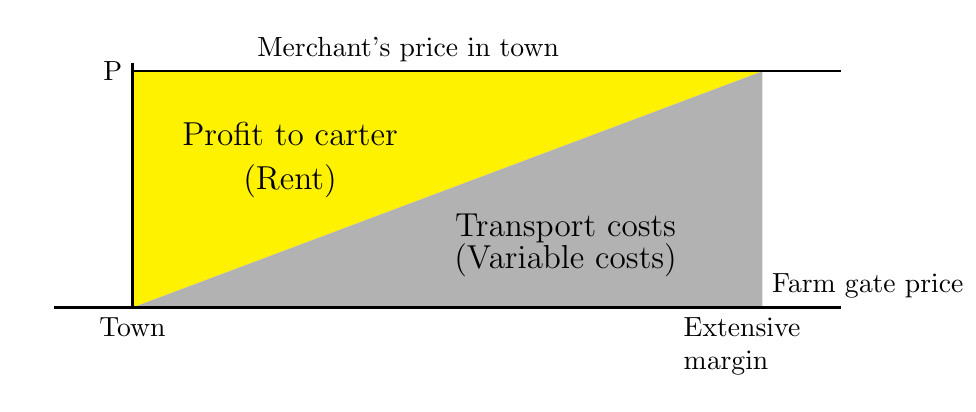
\begin{tikzpicture}[domain=0:2]
%\draw[thick,color=gray,step=.5cm, dashed] (-0.5,-.5) grid (3,3);
%\draw[line width=.01, green ] (0,0) -- (10,0) node[right  ] {Distance};
\node at (1,0) [below] {Town};
\fill[yellow]  (1,0) --(9,3)--(1,3) --cycle;
\fill[gray!60] (9,3) --(1,0)--(9,0) --cycle;

\draw[thick ] (1,3)node[left]{P}  -- (10,3);\node at (4.5,3)[above ] {Merchant's price in town} ;
\draw[thick ] (0,0)  -- (10,0); 

%\draw[thick,color=red] (1.5,0) -- (1.5,1) node[below right] {Fixed cost} -- (1.5,1.5) --(10,3.25)node[above left] {total cost};
\draw[thick] (1,0) -- (1,3.1) ;
\node[below,text width=2cm]at (9,0) {Extensive margin};
%\draw[ultra thick, blue,<-> ] (3,1.8) -- (3,2.5)node[left] {annual rent at a} -- (3,3) ; 
\node at (9,0)[above right] {Farm gate price};
\node  at (6.5,1){\large Transport costs};
\node  at (6.5,.6){\large (Variable costs)};
\node  at (3.,2.2){\large Profit to carter};
\node  at (3.,1.6){\large (Rent)};
\end{tikzpicture} 
    \caption{Transport costs, the yellow area, take a share of the profit for vegetables sold in the town}
    \label{fig-rent-ricardo}
    \end{center}
\end{figure}

At a certain distance, the transport costs will eat up all the profit on the trip. That is as far as the carter will go to buy potatoes. That distance is Ricardo's extensive margin. In figure \ref{fig-rent-ricardo}, total transport costs are shown as the yellow area. The area below the yellow triangle is profit for the carter. The carter makes a `profit' on the trip to the farm nearest to town, a declining profit as he travels away from town, and  no profit on any farms beyond this point.\footnote{Note the similarity with Alonzo's urban model, illustrated in Fig \ref{fig-rent-alonzo}.}
If the merchant's price went up, the extensive margin would move farther out, and more land would come into production.\footnote{This simple example assumes that the land is uniformly productive and that there is only one product that can be marketed. Johann Heinrich von Th\"unen, in The Isolated state (Der isolierte Staat (1826)), provide a more complex analysis based on the same principles \cite{GET_Johann_Heinrich}.} 

Together these two triangles/areas represent the net farm-gate value of the ``produce of the earth'', but only the lower triangle is surplus that can be allocated to the landlord, the carter, the mercheant or the consumeert.\footnote{It was termed the `\textit{produit net}' by the Physiocrats}. In modern supply and demand analysis it would be recognized as `producer surplus', the difference between what a producer gets for a good and what they would be willing to accept.

We have so far illustrated the story using a carter with a monopoly on transportation services. If instead there were a monopoly landowner, and the transportation industry were competitive, the landowner would pay carters their minimum cost and keep all the profits. In this case economists would call the monopoly profits rents.\footnote{In the modern economy, agricultural land rents may be captured by corporations,  either by owning the land or by controlling the supply chain.}  Landlord income in this example is a locational land rent that exists because of the land's proximity to the market.  

% ***E ADD?? This graph is simplified to illustrate the concept.
The land rent (that was profit) declines with distance from the town\footnote{It also declines for less fertile land, where there is a higher cost of production.}. At the extensive margin the land rent falls to zero. Even fertile land beyond the extensive margin will not be farmed because the product cannot be transported to market at a profit. Transportation costs and the price of produce in town determine the size of the  rent triangle and therefore the amount of rent captured by the land-owning class.\footnote{The debate about the  `Corn Laws" that Ricardo  was engaged in was about whether Britain would allow wheat from Canada and Australia to enter, reducing the price of wheat and therefore reducing the income and influence of the land-owning class.} 

%The profit now accrues to the landowner, and we call it land rent. For Ricardo, it was obvious that the land-owning class captured the land rent.

%\subsection{A more explicit treatment}
In 1902 Alvin Saunders Johnson \cite{johnsonRentModernEconomic1902} summarized the relationship between rent and surplus in the economic literature as follows: 

\begin{quotation}Of the concrete forms of income that have usually been classed as surplus, the rent of land was the earliest to be defined; and so prominent a position has been given to it that the terms "rent" and "surplus" have come to be used interchangeably.\end{quotation} 

\section{A changing economy brought a change in the theory of distribution}
As the economy shifted  moved from overwhelmingly  agricultural into the industrialization of the 18$^{th}$  and 19$^{th}$ century, economists shifted their focus from who got the rents to how prices and especially the prices of factors of production were determined. Rent theory was eclipsed by an approach that focused on the markets for the inputs used in industrial production.  Late in the 20$^{th}$ century, the focus shifted again, to the economics of  knowledge, human capital, and how cities generate wealth, a change that plays a part in  our theory of urban rents in Chapter\ref{chapter-growth}. 
 
 The changes have tracked changing social relations. The influence of landowners declined and the power of  industrial capitalists increased throughout the 19$^th$ century. More recently the owners of industrial capital have been eclipsed  by financial capital and, to some extent, by the owners or creators of certain information technologies.

\subsection{Marx}
%Ricardo, agreeing with Malthus, essentially assumes that the wage is  just sufficient to reproduce the labouring class.\footnote{``In the natural advance of society, the wages of labour will have a tendency to fall, as far as they are regulated by supply and demand; for the supply of labourers will continue to increase at the same rate, while the demand for them will increase at a slower rate.''} He then explains the distribution of the fruits of labour on the land among the main classes of the economy.
%***E ADD CONTEXT like:
Karl Marx (1818--1883)) was born three years after Ricardo published his Essay on the price of corn. 
By the time Marx was displaying  his developing interest in economics  at the radical newspaper, Rhineland News, Ricardo had been dead 20 years, the industrial revolution had been underway for almost a century and European economies were largely structured around manufacturing. 

 % ***E MORE ACCURATE TO SAY HE was exploring this because it was what he saw than shifted attention.
 In the manufacturing economy, the owners contribute the machinery, buildings, and even working capital to fund the workers until the product can be sold. % ***E FLESH OUT THIS DESCRIPTION OF THE KEY FEATURES OF TEH MANUFACTURING ECONMY. ALOS SPECIFCAL DEFINE CAPITAL CAN WHY IT MATTERS
 %This contribution must be accumulated from their profits in the preceding cycle of production,  and has to be reinvested once the revenues of the current round have come in and the bills have been paid. Marx actually describes a circuit of capital from its form as money to its form as physical capital. 
As in Ricardo, however, labour is in surplus and capital is scarce. As in Ricardo, the scarce factor is owned by a special class - now the capitalists - who are able to appropriate the surplus value. %Like Ricardo,  Marx saw the appropriation of surplus as without moral justification. 

Marx pointed to an additional dynamic feature of  capitalist systems - that productive capital is not fixed as land is, but  expands as surplus is reinvested. This creates an economy that can and, according to Marx, must grow, as well as challenges that are created by the capitalists' need to constantly reinvest their growing accumulation of surplus value. It was not until 1867 that  the first volume of Das Kapital,  was published, pulling together 20 years of Marx's analysis of the capitalist economy.  Das Kapital proposes an explanation of the "laws of motion" of the mode of production from its origins to its future by describing the dynamics of the accumulation of capital. With topics such as the growth of wage labour, the transformation of the workplace, capital accumulation, competition, the banking system, the tendency of the rate of profit to fall, and land-rents.% ***E EXPLAIN WHAT THIS MEANS AND WHY IT MATTERS TO DISTRIBUTION. HOW IS IT DIIFFERENT OR SIMLAR TO WHAT WAS HAPPENING UNDER FEUDALISM? 
%He famously suggested that the expansion will eventually outrun the expansion of demand and the rate of return will fall, leaving capitalists unwilling to invest. % and creating a crisis. 

***E FILL OUT CRISIS % WHEN i GET TO HENRY GEORGE AND YOU MAKE THE DISTINCTION BETWEEN HIS VIEW OF WHAT WOULD CAUSE CRISIS AND MARX'S, i AM CONFUSED BECAUSE YOU DON'T FULLY ARTICULATE THE PROBLEM. I THINK THIS IS SOMETHING MISSING HERE, BUT YOU COULD ALSO CHANGE THE LINE IN THE GEORGE SECTION IF THIS IS NOT AS IMPORTANT. TO ADD YOU WOULD JUST NEED TO EXPLAIN HOW THE NEED FOR GROWTH ULTIMATELY CREATES A PROBLEM OR CRISIS. WHY IS DOES IT POSE CHALLENGES. 
%***E I ALSO THINGK THAT THIS LIST OF TOPICS IN THE BOOK IS A BIT OF AN ABRUPT END TO EXPLAINING MARX'S CONTRIBUTIONS. IT WOULD BE HELPFUL TO PAINT MORE OF A PICTURE OF WHAT HE DOES WITH THESE TOPICS. INCLUDING THE CRISIS THING BUT ALSO A BIT MORE GENERALLY. THE TRANSITION TO HOW YOU POSITION MARX IS CURRENTLY A BIT ABRUPT. 


We see Marx as firmly part of the Classical tradition and a contributor to distributional theory.  Our work, linking urban rents to the dynamics of financial capital has one foot firmly  in the Ricardian and Marxian  tradition. Like Marx and Ricardo we explore how a particular type of surplus is distributed, how that might change, and the effect on society ***E OF THE VARIOUS SYSTEMS OF DISTRIBUTION?. Like Marx and Ricardo we find that a functional approach to social classes provides a useful framework. Where Marx focused on industrial \gls{capital}, however, we focus on capital in a different form: \gls{financial capital}% ***E SEEMS TO BE A LOT MISSING HERE?

% ***E i FEEL LIKE IT WOULD BE USEFUL TO DESCRIBE THE CLASS BREAKDOWN IN MARX AS IT RELATES TO HOW THE DIFFERENT ROLES FIT INTO PRODUCTION. aLSO. WHAT HAPPENED TO THE IDEA OF LAND RENT IN THIS PERIOD AND IN MARX'S WORK SPECIFICALLY? dID HE IGNORE IT? EVEN IF HE DIDN'T USE THE CONCEPT, EXPLAIN HOW IT WOULD RELATE OR FIT (OR NOT FIT) INTO THIS CONCEPT)
 
\subsection{Henry George} 
***E THIS SECTION FEELS A LITTLE SPARSE ON ECONOMIC ANALYSIS %YOU EXPLAIN GEORGE'S CONCLUSIONS VERY CLEARLY, BUT I FEEL THIS WOULD BE STREGTHEN A LITTLE MORE CLARITY ABOUT HOW HE RE-INTRODUCE LAND RENT. WHAT WAS THE ANALYSIS / iNSIGHT EXACTLY? THEN GO INTO THE CONCLUSIONS HE DREW ABOUT WHAT SHOULD HAPPEN...
In 1879, Henry George (1839--1897), an influential American political economist, published his most famous work, Progress and Poverty\cite{georgeProgressPovertyInquiry1973}. It sold millions of copies worldwide. George returned to land rent with a new insight based on the emergence of the capitalist city: the owners of urban land extract surplus in exactly the same way that owners of agricultural land do in Ricardo's analysis. ``With the growth of population, land grows in value, and the men who work it must pay more for the privilege.''  Where Marx saw the extravagant productivity of capital as the source of capitalist crises, George saw the extraction of wealth by land speculators as the mechanism that would bring on crises.
  % ***E WHAT DID HE MEAN BY CRISIS? HOW DID HE COME TO BE CONCERNED ABOUT THIS? ALSO SINCE YOU ARE COMPARING WITH MARX's PREDICTIONS ABOUT CRISIS YOU NEED TO EXPLAIN MORE ABOUT MARX'S IDEAS OF CRISIS ABOVE
  % ***E Somewhere in HERE YOU MAY WANTED TO EXPLAIN SOCIALISM VS MARXISM... GEORGE IS SOCIALIST? MARX?? PUTTING IN THE CONTEXT OF HOW THOSE TRADITIONS WERE EMERGING MIGHT BE HELPFUL... I HAD THIS NOTE ON THE PAPER DRAFT... COULDN'T FIGURE OUT WHY SINCE YOU DON'T SAY GEORGE IS A SOCIALIST. bUT YOU DO LATER WHEN YOU EXPLAIN THE SHIFTS IN jb CLARK'S THINKING. IF YOU WANT TO CONTEXTUALIZE CLARK IN TERMS OF SOCIALISM ... BEST TO MAKE SURE YOU'VE EXPLAINED THAT GEORGE IS A SOCIALIST, WHAT THAT MEANS, AND THEN, SINCE MARX IS FAMOUSLY BUT CONFUSINGLY INTERCONNECTED WITH SOCIALISM YOU SHOULD EXPLAIN HOW HIS THINK AND (SEPARATELY) THE MOVEMENT NAMED AFTER HIM FIT IN) 
  % # ADD George also presented solutions to ____ 
  
  Since land rent is not created by its owners, George argued that land rent should be seen as a social income - that it could be used to pay for all the needs of the community. The clearest statement of this view is found in Progress and Poverty when he wrote "We must make land common property." The same view was expressed by the Physiocrats who concluded  that ``ground rents'' should be the source of most or all taxes. They defined ground rent as that portion of all rent which is attributable only to the size and location of the parcel. George's analysis the `single tax' movement, which sought to shift all taxation to land  and resource rents.   

   
  In 1977, Joseph Stiglitz, using Alonzo's relatively new urban model, identified the conditions in which Henry George's "single tax" is  the only tax necessary to finance public expenditures.\footnote{Arnott, Richard J.; Joseph E. Stiglitz (November 1979). "Aggregate Land Rents, Expenditure on Public Goods, and Optimal City Size" (PDF). Quarterly Journal of Economics. 93 (4): 471–500. doi:10.2307/1884466. JSTOR 1884466. S2CID 53374401 }   The logic is fairly simple: if the public good increases productivity or the attractiveness of a city, attracting more people or businesses, land rents rise, and investment in the public good should proceed until the marginal cost of the public good is equal to the increase in land rent it brings. The result is now called the `Henry George theorem.'***E RELATE THIS TO YOUR THESIS. %I FEEL A BIT LOST IN WHAT YOU ARE SETTING UP HERE. COULD YO EXPLAIN HOW THEIS IS RELEVANT TO MODERN URBAN RENT THEORY? 
  
  ***E MAYBE MOVE UP THIS FOLLOWING PARAGRAPH? %THIS FEELS LIKE IT WOULD FIT WITH MORE DETAILED DESCRIPTION OF HIS ANALYSIS THAT I THINK SHOULD COME BEFORE HIS IDEAS ABOUT THE TAX. 
The classical economists agreed that rents are unearned income. They did not emphasize, as George did, that land rents arise from labour's proximity to urban population and production.\footnote{To be fair, it was not lack of understanding, that the omission reveals, but rather lack of interest in explicitly examining urban land rent from residential or even industrial purposes.}% Ricardo von Thunen, Marx, Cantillon all grasped the notion of proximity to the market as part of the source land rent. The discussions seem to not gone farther than discussions of diffeerential and rents, however.  I just am not aware of them explicitly examining urban land rent for residential or even industrial purposes. 

%The need to be near a market or prodduction center is easily seen by considering a population at the carrying capacity of the land with individuals supporting themselves using purely local resources. There can be no land rent in this case. If a city rises that must be supplied from those still on the land, land close enough to the city will generate land rent. The value of the land is created by proximity to the city.



%  no separate and comprehensive data are provided on the amounts of land rents and subsoil rents charged and earned, because they are not officially regarded as part of value-added, and consequently are not included in the calculation of GDP (except for the value of productive lease contracts)     https://en.wikipedia.org/wiki/Differential_and_absolute_ground_rent#Rent_in_macro-economics    \href{https://en.wikipedia.org/wiki/Differential_and_absolute_ground_rent#Rent_in_macro-economics}{Wikipediat article on differential rent}


  \subsection{John Bates Clark and neoclassical distribution theory}
  % # NEED SOME MORE CONTEXT HERE. maybe atart by setting up the PERIOD WE ARE NOW MOVING INTO AND WHAT HAS SHIFTED IN THE ECONOMIC STRUCTURE? 
  \epigraph{The law of rent has become an obstacle to scientific progress: it has retarded the attainment of a true theory of distribution. Yet it is itself capable of affording such a theory. The principle that has been made to govern the income derived from land actually governs those derived from capital and from labor. }{John Bates Clark \cite{clarkDistributionDeterminedLaw1891}}

Classical theories of distribution showed that ownership of a scarce and non-produced factor, land, was the  basis of rent extraction by the class of landowners. Profits were a bit puzzling for the classical economist because their connection to land rents was not as clear. Were profits just a part of land productivity captured by industrial producers as the earliest Classicals argued, or were they  additional  social surplus as the later Classical theorists thought? % ***E i DON'T UNDERSTAND WHY PROFITS ARE PUZZLING? WHATS THE QUESTION? eXPLAIN MORE. update: I STILL DON;T UNDERSTAND. 



Alfred Marshall (1842--1924)  one of the most influential economists of his time, and one of the founders of the school of neoclassical economics pointed out that, in a competitive market with free entry, scarcity profits (i.e., rent for capital) would normally be competed away  as entrepreneurs entered the market in pursuit of those `excess' profits. He used the term `quasi-rents' for these unearned but temporary incomes.\footnote{Alvin Saunders Johnson. Rent in Modern Economic Theory: An Essay in Distribution. AEA 3rd Series, Vol. 3, No. 4 (Nov., 1902), pp. 1-129 (129 pages)} This insight suggests that excess profit (profit over and above the normal rate of return on capital) unimportant in the long run, but left it an important short-run role in attracting existing capital to projects where it is most productive.\footnote{Contradicting Marshall, Carey and Lachim \cite{careySomethingNothingHow2019} observe that,``The persistent and growing profit share across a range of advanced economies and within industries fundamentally challenges the assumption of perfect competition and suggests that growing market power is at the heart of many of the economic challenges in America today.'' } 

As industrial production grew and eventually exceeded agricultural output 

% {\color{red}

%Adam Smith 
% A monopoly granted either to an individual or to a trading company has the same effect as a secret.… The monopolists, by keeping the market constantly under-stocked … sell their commodities much above the natural price … the price of free competition.…

% The exclusive privilege of corporations, statutes of and apprenticeship, and all those laws which restrain, in particular employments, the competition to a smaller number than might go into them, have the same tendency, though in a less degree. They are a sort of enlarged monopolies, and may frequently … in whole classes of employments keep up the market price of particular commodities above the natural price.… Such enhancements of the market price may last as long as the regulations of police which give occasion to them. wealth of nations
% }


John Bates Clark (1847--1938) was another of the pioneers of neoclassical theory and was one of inventors of the neoclassical theory of  distribution.  The neoclassical or marginalist approach emphasized that rational economic agents pay workers according to the value of the marginal product, the amount that the last worker hired added to output. % ***E DEFINE MARGINAL PRODUCT
 The same principle applied to other factors  
 Initially a socialist like George,   % ***E YOU NEED TO HAVE SAID ABOVE GEORGE IS A SOCIALIST OR CUT THIS. 
 by 1986 Clark was praising the dynamical process of competition and opposing the single tax movement George had initiated.  His (1891) ``Distribution as Determined by a Law of Rent,''\cite{clarkDistributionDeterminedLaw1891} argued that, given  competition and homogeneous factors of production labour and capital, the division of the social product will be according to the productivity of the last (or marginal) physical input of units of labour and capital.

Clark was correct, of course, but, by emphasizing that land and capital were factors of production like labour, he obscured the fact that it was not the capitalist or the landowner that contributed to production. It was the socially produced purchasing power or the land they held legal ownership rights over.\footnote{Clark, to be fair, also advanced the concept of social capital as a permanent, ongoing stream of future incomes out of which all productive inputs, including capital goods, are temporarily taken for a charge (interest). ``John Bates Clark''. Encyclopedia Britannica, https://www.britannica.com/biography/John-Bates-Clark. Accessed 1 March 2023.}  Responding to the ``indictment that hangs over society'' that it involves ``exploiting labour,'' Clark wrote:
    \begin{quotation}
        It is the purpose of this work (his 1899 'Distribution of Wealth) to show that the distribution of the income of society is controlled by a natural law, and that this law, if it worked without friction, would give to every agent of production the amount of wealth which that agent creates. However wages may be adjusted by bargains freely made between individual men (i.e., without labour unions and other "market imperfections", the rates of pay that result from such transactions tend, it is here claimed, to equal that part of the product of industry which is traceable to the labour itself; and however interest (i.e. profit) may be adjusted by similarly free bargaining, it naturally tends to equal the fractional product that is separately traceable to capital. 
  \end{quotation}
  
 In Clark's  perfect competition, % ***E I THINK YOU NEED A BIT MORE ABOUT COMPETITION AS A CONCEPT AND IT'S HISTORY. ITS PRETTY IMPORTANT. ALSO MAYBE REFERENCE ADAM SMITH ? 
 each factor of production—capital and labour—gets its just reward. That conclusion rests on a demanding set of conditions that we can only describe partially in this work. Perfect competition is an ideal type of market structure where all producers and consumers have full and symmetric information: everyone knows the true value of whatever they buy or sell.  This is a condition that may, at best, be satisfied in some markets. There must be large number of producers and consumers competing with one another. In fact, there must be large numbers in every market, whether for unskilled labour or specialist surgeon in the Yukon.  There have to be many suppliers of every drug, not to mention sewer services and electricity. there have to be new firms ready to enter the market  for any good  if the incumbents are making excess profits. There cannot be restrictive legislation. in the ideal case there can be no transaction costs -- hiring or firing a worker, for example,  is costless,  and there are no delays. The conditions required for a perfectly competitive economy are never met, but many commodity markets and some labour markets may come close enough to let economists treat them as competitive without risking making major errors. 
 % based on its contribution of  the last unit employed to a company’s profits. 
 A far more realistic description of the world is one of generalized  \gls{imperfect competition}, where the division of the economic pie is based not just on the relative contributions of capital and labour to the bottom line but on their relative scarcity, bargaining power and even political power.  % ***E THIS DOESN'T FEEL FULL EXPLIANED/JUSTIFIED. 
 % ***E YOU NEED TO EXPLAIN PERFECT COMPETITION AND WHAT IS ACCOUNTS FOR, EVIDENCE OF WHAT IT MISSES, ETC, THIS IS JUST A LOT OF ONE BRIEF PARAGRAPH TO COVER. COULD ALSO JUST REFERENCE PEOPLE WHO HAVE POINTED THIS OUT AS IF THIS IS WHERE ECONOMISTS ARE NOW, AND YOU ARE PICKING UP FROM THERE. 
 
Clark's analysis of income distribution does not contradict the classical view of rents, it simply displaces the analysis to the point where a competitive equilibrium prevails, and shifts attention away from the distribution of land rents. Rents are not earned by the marginal unit of land and therefore the share to land at the margin is zero. 
% ***E i STARTED TO FEEL LOST HERE, LIKE THERE IS A LOT MISSING SO ITS HARD TO FOLLOW. i THINK MAYBE THE SIMPLEST WAY TO FILL THIS SECTION OUT IS GOING TO BE TO TRACE WHAT OTHER ECONOMISTS SAY. LIKE THE NEO-CLASSICASTS SAID THIS THEN OTHERS POINTED OUT THE LIMITATIONS. THEN YOU POSITION YOURESLF AS RESPONDING TO ESTABLISHED ISSUES. 


%Even as Ricardo was writing, the industrial revolution was changing what Marx called the mode production changed. The influence of landowners declined and the owners of more liquid forms of capital became increasingly powerful. Thinkers like Marx and Engles revised and extended  class theory to account for growing power of the capitalists.  By the late nineteenth  century a new school of mathematically inclined economists focused on how competition regulated the distribution of wealth. They shifted the emphasis from ownership of the factors of production to the marginal product of the factors of production in competitive markets. It was eventually shown that the distribution under competition is, if not fair,  is at least efficient in a specific sense.\footnote{The result is known  in economics as the ``First Fundamental Theorem of Welfare Economics.'' The basic idea goes back to Adam Smith and was gradually developed  ver 70 years until Kenneth Arrow and Gérard Debreu (separately, 1951) each gave  a satisfactorily general proof in 1951. In 1986 %their 1986 paper, ``Externalities in Economies with Imperfect Information and Incomplete Markets''
%Bruce Greenwald and Joseph Stiglitz showed that the fundamental welfare theorems do not hold if there are incomplete markets or imperfect information.}
MOVE DOWN suppressed as a concept as though it appears in a huge number of contexts, thought not under the name, but it appears not in the clasical
% drop land out of neoclaclasical analysis since were not focuse on fixed/unchangible factors

 Modern economists generally focus  on the exchange price and the marginal conditions satisfied in exchange, which neoclassical economics explains more satisfactorily They appear to have abandoned rents as a central concept, but it  persists in slightly covert forms at the centre  neoclassical economics. 
\begin{enumerate}
    \item Alfred Marshall identified industrial profits as a form of rents, terming them `quasi-rents'' to emphasize that, unlike land rents, industrial profits would  be expected to disappear over time as new firms entered the industry.]
    \item First year students are taught that the high salaries of  sports stars are rents on their scarce talents. 
    \item First year students also learn about ``consumer surplus'' and ``producer surplus'' in supply and demand analysis. Both of these concepts are variants of rent and are essential in demonstrating the efficiency of a markets and the social losses due to monopoly, monopsony, regulation, and taxes. Consumer surplus is the sum of rents that accrue to the class of consumers (buyers). It is an inframarginal quantity, like land  rent, that accrues to the class of landowners. It arises because consumers have differing capacity to produce  utility with the good, just as landowners have lands with different abilities to produce agricultural output. Producer surplus corresponds precisely to land rent in Figure~\ref{fig-rent-ricardo}.  

    
 \begin{figure}[h!]
\begin{center}
 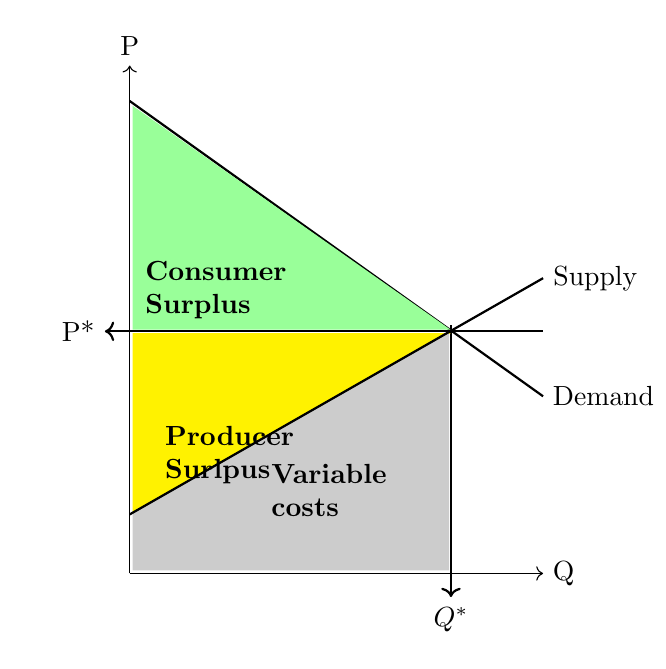
\begin{tikzpicture}[scale=1.5]
%\draw[thick,color=gray,step=.5cm, dashed] (-0.5,-.5) grid (3,3);
\draw[->] (0,0) -- (3.5,0) node[right ] {Q};
\draw[->] (0,0) -- (0,4.3) node [above] {P};
\draw[thick] (0,4) -- (3.5,1.5) ; \node [right]at (3.5, 1.5 ) {Demand}; 

\draw[thick,->] (2.72,2.1) -- (2.72,-.2) node[below] {$Q^*$};
\filldraw [color=green!40]  (0.03,2.07)-- (0.03,3.95)--(2.7,2.07)--cycle;
\filldraw [color=yellow] (0.03,2.03)-- (0.03,.515)--(2.7,2.03)--cycle;
\filldraw [color=gray!40](0.03,.515)--(2.7,2.03)-- (2.7,0.03)--(0.03,0.03)--cycle;
\draw[thick,<-] (-.21,2.05)node[left]{P*}  -- (3.5,2.05) node[above left] {}; 
%\fill[blue, opacity=.25]  (0,4) -- (1.86,2.1) --  (0,2.1) --cycle; 
%\fill[green] (0,.52) -- (1.82,2.1) --  (0,2.1) --cycle; 
\draw[thick] (0,.5) -- (3.5,2.5) node[right] {Supply};
\path (.7,2.4) node [text width=1.7cm](labelRent) {\textbf{Consumer\\ Surplus}};
\path (.8,1.) node [text width=1.5cm](labelRent) {\textbf{Producer\\ Surlpus}};
\path (1.7,.7) node [text width=1.5cm](labelvarcost){\textbf{Variable\\ costs}};
%\path (1.7,-1) node [black](labePC) {With producible capital};
  \end{tikzpicture}     
\caption{The basic supply and demand model determines price and quantity }
\label{fig:Equilibrium}
\end{center}
\end{figure}

    \item The First Fundamental Theorem of Welfare Economics, proven independently by Kenneth Arrow \cite{arrowExtensionBasicTheorems1951}and  Gerald Debreu \cite{debreuCoefficientResourceUtilization1951}  in 1951, possibly the most significant theorem in the social sciences,   demonstrates that perfectly competitive markets would maximize producer and consumer surplus, quantities that really are variants of rents.
    \item The ``\gls{bid-rent curve}'' became a dominant device  in urban theory with William Alonzo's 1961 thesis \cite{alonzoTheoryUrbanLand1960}, although the idea has deep roots and others were exploring the principle at the same time.  
    \item The theory of ``\gls{rent-seeking}''   became the subject of durable interest among economists and political scientists after the publication of two influential papers on the topic by Gordon Tullock in 1967 \cite{tullockWelfareCostsTariffs1967}, and Anne Krueger \cite{kruegerPoliticalEconomyRentSeeking1974} in 1974. Rent-seeking occurs when an someone seeks to increase their own wealth without creating any benefits or wealth to the society. Financialization, as we use the term, is a variety of rent seeking
\end{enumerate}
% In neoclassical economics, however, the focus is on the exchange price and the marginal conditions satisfied in exchange, which neoclassical economics explains more satisfactorily than the classical approaches did.  

%We do use their approach to distributing the distribution of the productive surplus to workers. - 

\section{Summary}
We have examined the main stages of rent and distribution theory 
% as  a bridge from classical rent theory to the
as the necessary background for our development %extension 
of the modern theory of urban rent. On the way we explained how the concept of economic rent arises in an agricultural economy, and who gets the rents in that type of economy. We then gave an account of how rent theory and the classical distribution theory was pushed into the background as neoclassical theorists analysed the industrial market economy that emerged after the industrial revolution. In the next chapter we introduce 20$^{th}$ century urban models that are essentially an application of Classical rent theory.

% The distribution of rents in the urban model affects urban productivity in our model.

%***E FINANCIALIZATION IS ABOUT SURPLUS. CURRENT THINKING ABOUT FINANCIALIZATION HAS NOT BEEN NOT BEEN PUT INTO A FORMAL MODEL. FORMAL MODELS COME FROM COME FROM THE NEO-CLASSICAL TRADITION. 
\chapter{Urban Land and Land Rent} \label{chapter-space}

\epigraph{Overall, several decades after its creation, the standard urban model seems to still capture surprisingly well the inner structure of many cities across the world, both in developed and in developing countries.}{Liotta et al. 
 \cite{liottaTestingMonocentricStandard2022}}

%who is trying to solve what kind of problem

%MAKE ALONSO A CHARACTER, AND INTRODUCE HIS PROBLEMS
% A large part of the surplus appears as locational rents, so we then go to developing the spatial and urban model in which rent operates.  
% URBAN MODELS ARE ROOTED IN CLASSICAL NOTIONS OF RENT, FOLLOW A SIMILAR LOGIC TO RICARDOS EARLY AGRICULTURAL MODEL.
% WHAT ARE THEY MODELLING
% WHAT QUESTIONS WERE THEY DEVELOPED TO EXPLORE/ANSWER
% WHAT IS THE CONTEXT/PERIOD/SOCIETAL CONDITIONS THAT PROVIDED THE CONTEXT FOR THESE TO EMERGE IN? 
% DOES WEALTH/RENT/PRODUCTION FIT INTO THE MODEL? WHAT IS INCLUDED BEFORE WHAT IS NOT INCLUDED
% SOMETHING LIKE RENT OR RELATED TO RENT SEEMS TO BE PART OF THEM... DID THIS COME FROM RENT? OR TO ANSWER SIMILAR QUESTIONS? OR DOES IT COME FROM A DIFFERENT DIRECTION BUT MODEL SIMILAR? 
% WERE THEY ANSWERING THE SAME QUESTIONS
% WHAT WERE THE QUESTIONS ABOUT CITIES AND SPACE THEY WERE TRYING TO ANSWER? 
% WHAT SPECIFIC SPATIAL.URBAN FEATURES WERE IN THE MODELS

% The s tudy of space is huge, and seeping into those few fields it hasn't infiltrated. 

% Urban modelling, done by planers geographers and econoists. It tends to focus on transportation, the study of space. The fiedl is space. locations of people, housing forms, the demographic and form of the field

% urban modelling is a sub discpline. There ar programs of urban economic it's a subfield of regional science/regional economics.

% Modeling location, spatial value, locations represents a sub-feids in regional science and a sub-field in economics. A model which brings the two closer together is the Alonso model. It's dominant feature.

% DON'T EXPLAIN WHAT AN URBAN MODEL IS AT ALL. WHAT IS THE CONTEXT, WHAT QUESTIONS ARE THEY TRYING TO ANSWER. 
% SOUNDS LIKE THEY ARE TRYING TO DO THE SAME THINGS AS ECONOMISTS DO WITHOUT THE SAME TOOLS. 
% THEY DON'T HAVE THE SAME PROBLEMS.


% The financialization of housing is a spatial process. %Rent as we've talked about it is an urban process, but we need a more explicit understanding of land. 
% It occurs

% The early 1960s were a watershed in urban economics. Land rent theory returned to economics and \gls{regional science} in the form of a new model of urban structure  that linked the urban wage premium to urban land rents through transportation costs. The model rapidly became the workhorse for theorists and empirical researchers. It helped explain land prices, the built form of the city, and where people live relative to where they work, using a logic analogous to Ricardo's theory of rent, as it appeared in the story of the carter carrying farm products to market in Section~\ref{section-rent-carter}), applying it to a city where workers commute to jobs. % (TRIED EXPLAINING A FEW OF THE THINGS IT GAVE INSIGHT TO  MAKE THIS MORE CONCRETE, BUT IT MIGHT BE BETTER TO MENTION SOMETHING ELSE? FEEL FREE TO CHANGE/REMOVE.)



% THIS IS AMAZING!! MAYBE NOTE THAT IT DIDN'T BRING FORWARD DISTRIBUTIONAL ASPECTS HERE? I THINK IT WOULD HELP TO SAY WHAT REGIONAL SCIENCE IS/HOW IT IS DIFFERENT FROM URBAN ECONOMICS.

\section{Intro 2}
The discussion of rent in the previous chapter provides the necessary economic logic that underlies the analysis of this thesis, but we are interested in the application of rent theory to the modern urban economy. For that we draw on relatively recent models from urban economics and urban geography. Economic geography in general is the use of the tools of economics to analyze locational decisions. Applied to urban areas, it takes up urban issues such as crime, education, public transit, housing, land use restrictions, local labor markets, agglomeration economies, trade, transportation infrastructure, and local government finance. 

The early 1960s marked a watershed for the field.  Alonso (1964), Mills (1967) and Muth (1969) introduced a theory of the internal structure of a city that explains land values in terms of transportation costs. The goal of this chapter is to describe informally the now classic and dominant spatial urban model that that emerged at that time. It serves in our analysis as the link between rent theory and financialization. % we will use. 
We will review the theory and development of the core urban model and discuss how it uses urban land rent to explain urban size and structure. % to our analysis. These models (From: Handbook of Regional and Urban Economics, 2004) 

The new  model of urban structure linked the urban wage premium to urban land rents through transportation costs.  It rapidly became the workhorse for theorists and empirical researchers. It helped explain land prices, the built form of the city, and where people live relative to where they work, using a logic analogous to Ricardo's theory of rent, as it appeared in the story of the carter carrying farm products to market in Section~\ref{section-rent-carter}), applying it to a city where workers commute to jobs. 


What we refer to the basic model is often called the Alonso model, although it  was developed by several scholars working in parallel in parallel in roughly the same period. William Alonso published \textit{Location and Land Use} in 1964  \cite{alonsoLocationLandUse1964} based on his 1960 PhD thesis \cite{alonsoModelUrbanLand1960},  
giving him a slender priority in the literature. 
Richard Muth's \cite{muthSpatialStructureHousing1961}, and \cite{muthRationalExpectationsTheory1961} were written roughly simultaneously with and independently of Alonso's thesis, and culminated in Muth's classic book, Cities and Housing  \cite{muthCitiesHousingSpatial1969}.\footnote{See ``William Alonso, Richard Muth, Resources for  the Future, and the founding of urban economics''\cite{mcdonaldWilliamAlonsoRichard2007} for a more detailed discussion of the development of the model.}  % ***E ADD % This workoverlps with Alonso in these ways. Differed in these ways \dots USE THIS TO FLESH OUT MORE OF THWAT HIS MODEL?WORK ISDOING AND HOW
% We will refer to the core urban model developed by 
 The model was developed further by Muth \cite{muthCitiesHousingSpatial1969} and Mills \cite{millsAggregativeModelResource1967}, and later formalised by Wheaton \cite{wheatonComparativeStaticAnalysis1974}.\footnote{it is also called the Alonso model, the Alonso-Muth model, the Alonso-Muth-Mills model, the circular city model, and the monocentric city model.} %(***E ADD \dots % He was concerned with \dots His model did \dots INTRODUCE THE WORK ITSELF) 
\footnote{It is worth noting that Lowdon Wingo also had what appears to be a working paper, \textit{Transportation and Urban Land} \cite{wingoTransportationUrbanLand1961}, for the organization Resources for the Future  in preparation for publication that presented a core idea and  significantly influenced Muth \cite{mcdonaldWilliamAlonsoRichard2007}.} Mills' \textit{Urban Economics} \cite{millsUrbanEconomics1972}. followed soon after. 

The model is built around an extremely simple trick for calculating what people will bid or pay to live at a particular location  called the \gls{bid-rent curve}. That amount is a locational rent of the sort Ricardo discussed in the context of an agricultural economy.  

Starting with the fact that a worker is more productive in the city, the worker should receive a wage premium, $\omega$, for working in the city. That premium has to cover the cost of commuting to work, so the amount of the  wage premium left as a benefit for the urban worker must decline with distance from the workplace. 

But notice this additional point: if workers are renting their homes, landlords can charge a premium for being closer to the center of the city where transportation costs are lower.  Landlords can capture a share of urban productivity. How much can they charge? How much will a worker bid for a rental? The maximum charge is the part of the wage premium left after transportation costs are paid. If landlords are at all greedy, that is also the minimum they will charge. 

We can write a very simple formula for the surplus  value at any point $d$ from the centre of the city. This value is called the bid-rent  $mathcal{R}$: 
\begin{equation}  
\mathcal{R}= \omega - dc \label{eqn-bid-rent}\end{equation}
where $d$ is the distance from work and $c$ is the transportation costs.\footnote{ if the wage is paid monthly then $c$ has to be the monthly transportation cost.} Equation~\ref{eqn-bid-rent} describes a downward-sloping line (a curve) that is known as the bid-rent curve. The bid-rent curve is the key to the Alonso model.\footnote{We are describing the simplest possible version of the model. There are many excellent versions that incorporate complex spatial geography, multiple spillover effects, and other features-- see for example \cite{ahlfeldtECONOMICSDENSITYEVIDENCE2015} for an example and extensive references---, but our focus is on the effects of financialization, so we use the minimal model to bring out effects that would be more difficult to disentangle in a more complex model. Qualitative results should be unaffected by this simplification.}   

The \gls{bid-rent curve} represents a special  kind of economic equilibrium:   a locational equilibrium among mobile households. Since individuals would simply move to any location that offered a higher utility, in an equilibrium all the otherwise identical workers must receive the same utility. This has to be the case even though those farther from the center must pay more for transportation to and from home. The variable that  adjusts to maintain equal utility with rising transportation spending is the cost of housing. This conception of a \gls{locational equilibrium} is what underlies the bid-rent curve and all its extensions.\footnote{For economists it is also described as a Nash equilibrium.}


The seeds of the \gls{bid-rent curve} that is  at the heart of the model were presented as early as 1885  by German engineer-economist Wilhelm Launhardt \cite{blaugEconomicTheoryRetrospect1985, launhardtMathematischeBegruendungVolkswirthschaftslehre1885}. The  \gls{bid-rent function} was first applied explicitly to the equilibrium of land use patterns in agricultural production by August Losch \cite{loschEconomicsLocation1954} in Germany and later by Edgar S. Dunn \cite{dunnEquilibriumLandUsePatterns1954} in America. It was not until the 1960s that it was discovered that it could be applied  to the urban setting by Alonso and others. It was then very quickly recognized as a fraternal twin of August von Th\"unern's 1826 agricultural planning model \cite{vonthunenIsolirteStaatBeziehung1826}. von Th\"unern actually wrote down a version of Equation~\ref{eqn-bid-rent}. With the work of Alonso and his contemporaries, the classical concept of land rent  moved  from  agricultural economics to the centre of the modern urban economy.  


% https://press.uchicago.edu/ucp/books/book/distributed/C/bo23348570.html Macy Conference
% https://archives.library.illinois.edu/thought-collective/cybernetics-thought-collective/
% Norbert Wiener published Cybernetics in 1948
% Margaret Mead and Gregory Bateson


% "The Macy Conferences on cybernetics brought together a diverse host of scholars, including Margaret Mead and Gregory Bateson (anthropology), Warren S. McCulloch (neurophysiology), Heinz von Foerster (physics and electrical engineering), Norbert Wiener (mathematics), W. Ross Ashby (psychiatry), John von Neumann (computer science), Claude Shannon (mathematics and electrical engineering), G. Evelyn Hutchinson (ecology), and Arturo Rosenblueth (physiology). While these scholars met together at the conferences on a few rare occasions, they used a variety of other means to create and foment a community—a Denkkollektiv, or a scientific “thought collective”—around cybernetics. As defined by scientist Ludwik Fleck in his influential publication Genesis and Development of a Scientific Fact, a thought collective is a “community of persons mutually exchanging ideas or maintaining intellectual interaction” (Fleck, 1979), and the cybernetics thought collective subsisted during the three decades that followed the Macy Conferences.


 Bruckner \cite{bruecknerStructureUrbanEquilibria1987} describes the resulting model as ``a simple yet powerful model of urban spatial structure that successfully explains the principal regularities observed in the urban landscape,'' and goes on to say ``the good predictive performance of the model suggests that its simplifications are artfully chosen, capturing the essential features of real-world cities.'' It remains the central model in modern urban economics.

The models don't however bring forward the distributional and class features derived by the classical economists. They don't examine distribution or how the distribution of rents might affect the productivity of the city, which means they throw no light on the effects of financialization of the property market on distribution or on urban productivity. 
In this thesis we  explore who gets the urban land rents and how that is changed by the financialization of urban housing.

% Standard urban models are based on spatial rents, and follow directly from the theory of rent developed in Ricardo.
% As discussed in the previous chapters, 
% Modern urban models apply classical rent theory to understanding the structure of the city. %are essentially an application of classical rent theory. 


% HENRY GEORGE applied to cities, urban models formalized the concept.
% Although the model is easily generalized, we restrict our presentation to the highly stylized core version to establish how land rents are generated in the urban system and how they are related to neoclassical growth theory. 


% \section{From Ricardo's rent to Alonso's urban model}

% The Alonso model extends the approach developed in Ricardo approach to rent to the urban system, and is % Alonso's spatial model is 
% rooted in the classical notion of rent. 



\section{From Ricardo's rent to Alonso's urban model}
The Alonso model  re-presents Ricardo's conception of rent mathematically for a different social system and production technology. Ricardo had described a model with a central market for an agricultural product like potatoes. Producing potatoes took land and transporting potatoes to market was costly. Because there is one market price for potatoes, land with low transportation costs near the central market earns a rent. More distant land has lower value for farmers. In Alonso's model there is central market and a single price for labour, producing labour takes land, and transporting labour to the market is costly. Rent emerges from the scarcity of space close to the labour market at the city core, just as  in Ricardo it emerges from the scarcity of land near the market for potatoes and grains. 

The new urban models models exploit the relationship between rent and location  described in  Equation~\ref{eqn-bid-rent} to explore the spatial structure of the city. Figure~\ref{fig-alonso-simple} illustrates the simplest case. We are looking at a thin slice of the city from the centre to its edge at $d^*$. The vertical dimension is dollars of rent or transportation cost.  Notice that rent and transportation cost sum to $\omega$. 

We assume in this simple model that the city sits on a uniform plane and has a population of identical workers with identical housing needs, and identical transportation costs who all work at the city centre and receive the same wage. We also assume, as is common for simple versions of the model, that the labour market and production sector at the centre take no space. 

As above, transportation to and from the center costs ${c}$ times the distance $d$ from the center.\footnote{Fuel, capital, and time costs are  all included in the transportation costs, ${c}$. } The diagonal line is the bid-rent curve. The figure shows  bid-rent declining with distance from the centre and transportation cost rising. Property values at any point are a multiple of the rent at that point.\footnote{In this model they are simply the capitalized (present discounted) value of the stream of rent. Amenities, taxes and building values all modify the value calculation in more realistic cases.} At $d^*$ transportation costs completely absorb the wage premium. There is no surplus that the landlord can extract.\footnote{In many discussions of the model it is assumed that beyond $d^*$ the best use of the land is for agriculture since it cannot earn a rent premium. }

% %%%%%%%%%%%% PARTITIONING THE LABOUR SHARE
\begin{figure}[!ht]
    \begin{center}
    
% Simple Alonzo model
%%%%%%%%%%%%%%%%%%%%%%%% PARTITIONING THE LABOUR SHARE
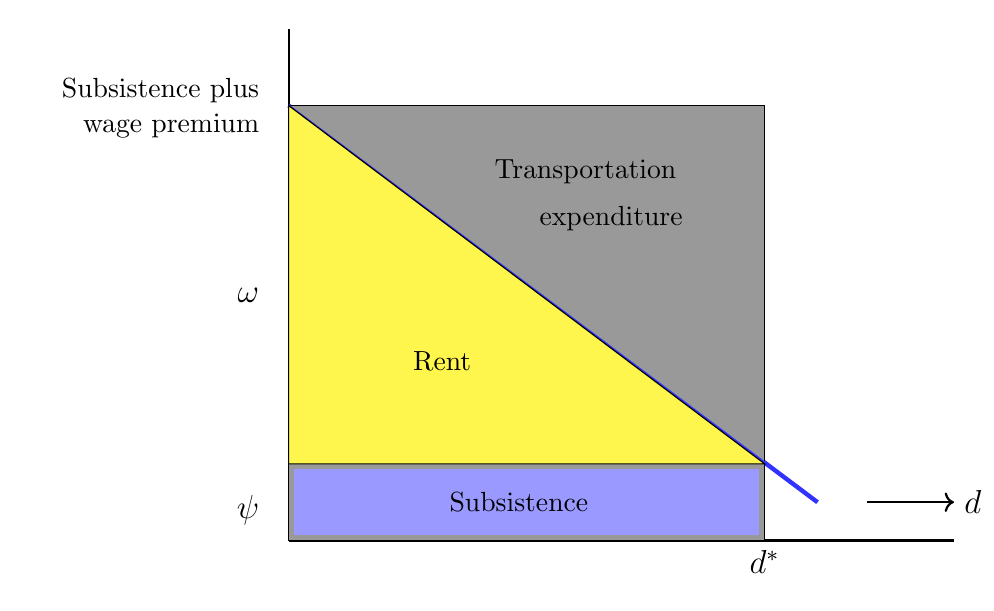
\begin{tikzpicture}[scale=.65]
\def\bndmax{5}        %https://tex.stackexchange.com/questions/68462/filling-a-complex-region-with-tikz
\def\bndmin{0.2}
\def \n {8.5}  % height of y axis
\def \d {13}  % length  of x axis
\def \t {.75}  %  cost of transportation per unit x
\def \th {1}   %
\def \w {7}    %  wage premium
\def \om{1.5}%  omega =rural wage Zero for urban population
\def \azero{2}
\def \aprime {-.0}	
\tikzset{func/.style={thick,color=blue!80}}	

% FIRST FIGURE just axes PARTITIONING THE LABOUR SHARE
\draw [thick] (0,-\om) --(\d,-\om);  			% Zero for rural population
\draw [thick] (0,-\om) --(0,\n); %node[above]{\Huge $w$};	% Y axis
%\node at (0,\n+0.5){\large $Rent$};

% \draw [thick] (0,0)node[left=.5]{Subsistence}--(\d,0);
%\node at(-2,1) {$\omega$};
\node[left=.25] at (0,3.3){\large $\omega$};
\node[left=.25] at (0,-0.9){\large $\psi$};
%\node[left=.25] at (0,3){$w+\omega$};
\node[left=.25] at (0,\w+.3){Subsistence plus};
\node[left=.25] at (0,\w-.4){wage premium};	

%\foreach \xi in {0,..., \n} \draw (\xi,0)--(\xi,-.1)node[below=1]{\small$\xi$};
%\foreach \yi in {1,...,\n} \draw (0,\yi)--(-.1,\yi)node[left]{$\yi$};
%\foreach \i in {1,4,9,16} {
%\node at (7,-\om/2){people scattered uniformly across the land  };

%SECOND FIGURE WITH AGGLOMERATION WAGE
%   \pause %  add urban production and net wage PARTITIONING THE LABOUR SHARE
%\draw[fill=white, white] (0.1,-0.1) rectangle (14,-\om+.1);
%\draw [fill=green!80] (-.25, 0) rectangle(.25, \w);
\node[right] at  (.25, \w/2){Added Productivity};
% \node[right, text width = 3cm] at  (10,9){Where does the increase in productivity come from?};
\draw [ thick, ->](11.3,-\om/2)--(13, -\om/2)node [right] {\large $d$};

%  THIRD FIGURE  add wage profile PARTITIONING THE LABOUR SHARE
% \pause
%\node[right, white, fill=white,  text width = 3cm] at  (10,9){Where does the increase in productivity come from?};
\draw[func, domain=0:\w/\t+1,ultra thick] plot [samples=200] (\x,{\w-\t*\x}); %Net wageprofile  for 
%\node[right, white, fill=white] at  (.25, \w/2){Added Productivity};
%\node[right, fill=white, text width =3.5cm ] at  (1, \w/2){Declining wage  net \\of transportation\\ costs $T(d)$ };

%   FOURTH FIGURE     commuters PARTITIONING THE LABOUR SHARE
%\pause
%\draw[fill=blue!40] (0.1,-0.1) rectangle (9.2,-\om+.1);
%\node at (4.5,-\om/2){commuters};

%   FOURTH FIGURE    wage bill
%\pause %add total new value
% \draw[fill=green!40] (0,-\om) rectangle(9.30,\w);% new product
% \node at (4.5,\w/2){\Large urban wage bill};

%%   FIFTH FIGURE   distribution
%\pause
%\node at (9,\n){\Large Partitioning the Labour Share};

\draw[fill=black!40] (0,-\om) rectangle (9.30,\w);% new product repeat
\draw[func, domain=0:\w/\t+1] plot [samples=200] (\x,{\w-\t*\x}); %rent profile
\fill[blue!40] (0.1,-0.1) rectangle (9.2,-\om+.1);
\node at (4.5,-\om/2){Subsistence};
\draw[fill=yellow!70,] (0.,0.) -- (0,7)--(9.30,0.)--cycle;% Rent \w-.2
\node at (3.,2){Rent}; 		%Rent 
\node at (5.8,5.7){Transportation};
\node at (6.3,4.8){expenditure};
\node at (9.3,-1.5)[below]{ \large $d^*$};
% \node at (4.8,\w)[above]{\huge $d^*$};
 \end{tikzpicture}
 

    \caption[The allocation of worker income by distance from the centre of the city.]{The allocation of worker income by distance from the centre of the city, where $\psi$ represents the \gls{subsistence wage}, which is the same as the rural income, and $\omega$ represents the \gls{urban wage premium}, which is paid out of the increased urban productivity resulting from agglomeration.}
    \label{fig-alonso-simple}
    \end{center}
\end{figure}

 

In Figure~\ref{fig-alonso-simple}, the height of yellow triangle $\omega$ represents the wage premium $\omega$ for urban labour and the amount land rent earned at the centre % of the city.  at the centre, 
where transportation costs are zero. The entire yellow triangle is aggregate land rent generated by the city along a section from the centre to the edge. 
The model says nothing about who gets the rent in the urban economy. 
For classical economists it was obvious that the agricultural rents went to the class of land-owners, as discussed in Chapter~\ref{chapter-rent}. 
For us it is a question to examine, since it depends on who owns the land.  Transportation cost depends on the distance  to and from the center.  
The gray triangle represents the aggregate transportation expenditure by residents along a section from the centre to the edge. 
The entire rectangle, $\omega$ $\times$ $d^*$, is the wage bill generated by urban agglomeration for the workers on the strip of land illustrated. Urban land rent is the residual when transport costs are deducted from the wage premium. %It declines with distance $d$ until, at the edge of the city, $d^*$, the cost of transportation consumes the entire wage ($d^*{c}=\omega$, where ${c}$ is the transportation cost, including fuel, capital, and time costs. The grey triangle represents the amount of the surplus dissipated in travel costs.  Property values are simply the present discounted value of the rent at any point.

At the bottom of the figure we add a `subsistence wage'  earned by a worker whether in the city or outside of the city. In most analyses of urban spaces, this living wage is simply ignored, since it is the wage premium that generates rents.  The relative size is unimportant because it is the same for urban and non-urban workers. If urban consumption is higher than non-urban consumption it must come out of the land rent.
% Workers are attracted to the city by the wage premium, $\omega$,  which represents the share of the surplus generated by the city that goes to labour.  

% The extent  of the city  $d^*$ is  simply the distance at which total $rt$ transportation cost  is equal to the wage premium
% \[d^*{c}= \omega\]
% where ${c}$ is the unit cost of transportation. In the figure, $-{c}$ is the slope of the diagonal line dividing rent from transportation expenditure.

 \subsection{The magnitude of rents and transportation costs}
 From $\omega$, $c$ and population density we can derive population, wage bill, total rent, and transportation costs. The figure above suggests that  half of the urban surplus is spent on transportation, but that is because the figure makes it appear that the city is stretched out in one dimension. If  the city is circular, the total value of rents can be represented as  a cone with radius $d^*$, height $\omega$ and volume  \[ V=\frac{1}{3}\pi  d^{*2} \omega \]
Since $d^*=\omega/c$ we can substitute out either  $\omega$ or  $d^*$ to show that total rent is  proportional to the cube of either  $d^*$ or $\omega$. 

The total value of wage payments appears as the volume of the cylinder enclosing the cone since the wage is the same for each unit of labour no matter where it resides: 
$V=\pi r^2 \omega$. This is generally a fraction of the value of the city's agglomeration economies. 
Total transport costs are $\frac{2}{3}\pi  d^{*2} \omega).$
With uniform density, the population is proportional to the square of  $d^{*2}$ while rents and transportation costs are proportional to the cube. %move this?

% BID-RENT MEANS

\begin{figure}
    \begin{center}
    
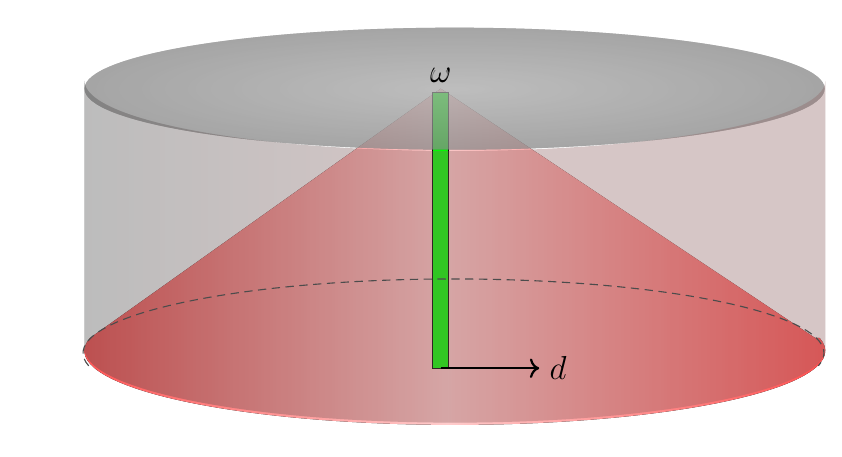
\begin{tikzpicture}[scale=.5]
   %%%%%%%%%%%%%%%%%%%%%%%%%%%%%%%%%%%%%%%%%%%%%%%%
% definitions for schematic
\def\bndmax{5}        %https://tex.stackexchange.com/questions/68462/filling-a-complex-region-with-tikz
\def\bndmin{0.2}
\def \n {10}  % height of y axis
\def \d {12}  % length  of x axis
\def \t {.75}  %  cost of transportation per unit x
\def \th {1}   % theta?
\def \w {7}    %  wage premium
\def \om{1.5}%  omega =rural wage Zero for urban population
\def \azero{2}
\def \aprime {-.0}	
\tikzset{func/.style={thick,color=blue!90}}	

    %%%%%%%%%%%%%%%%%%%%%%%%%%%%%%%%%%%%%%%%%%%%%%%%
% definitions for Cone3
%\node at (0, 2.5){\input{SA_Cone3.tex}};
     \pgfmathsetmacro{\radiush}{9.7};%Cone base radius was 9.6
        \pgfmathsetmacro{\theight}{7.1}%Cone height (negative if you want a inverse cone)
        \pgfmathsetmacro{\cheightp}{.03}%Cut height in percent of cone height

        %Calculating coordinates
        \coordinate (center) at (0,0);
        \pgfmathsetmacro{\radiusv}{.2 * \radiush}; %HORIZONTAL RADIUS
        \coordinate (peak) at ($(center) + (0,\theight)$);     
        \pgfmathsetmacro{\sradiush}{\radiush * (1 - \cheightp)};%ADJUST FOR COVERAGE AT CORNERS
        \pgfmathsetmacro{\sradiusv}{.2 * \sradiush};
   %     \pgfmathsetmacro{\sradiusv} {\sradiusv -.1 };

\coordinate (antipeak) at ($(center) + (0,-\theight)$);  %thanks  %I added this
\coordinate (vert1) at ($(center)+(\radiush,-.2)$);
\coordinate (vert2) at ($(center)-(\radiush,.2)$);
%problem
   
\coordinate (svert1) at ($(vert1)!\cheightp!(peak) +(0.1,.75)$);
\coordinate (svert2) at ($(vert2)!\cheightp!(peak)+(.5,.75)$);  
    % \coordinate (svert3) at ($svert1+(0,\w)$);
    % \coordinate (svert4) at ($vert2)+(0,\w)$);  
    %  \coordinate (svert3) at ($svert1+(0,7)$ );  % Shifting up by W
    % \coordinate (svert4) at ($svert2 + (0,\w)$0;
   %%%%%%%%%%%%%%%%%%%%%%%%%%%%%%%%%%%%%%%%%%%%%%%%


 
%\draw[step=.5,black,thin] (-9.6,0) grid (9.6,7);
 
% Cone Drawing    
 \fill[ left color=red!70, right color=red!70,  opacity=20,middle color=red!20,shading=axis] (svert1) -- (peak) -- (svert2) arc (170:370:\sradiush cm and \sradiusv cm);

    % FAT GREEN BAR
 \draw [fill=green,opacity=80] (-.2, 0) rectangle(.2, \w);
 \node[above] at (0,\w){$\omega$};
 
%Uncomment this for top of cylinder
      \fill[inner color=gray!2,outer color=gray!40,shading=radial,opacity=.5] ($(center) + (.35,\theight)$ ) circle (9.4 cm and 1.55 cm );
      
        % \draw [thick]($(svert1) +(.3,-.3)$)-- ++ (90:\w-.2);
        % \draw [thick]($(svert2)-(.2,.3)$)-- ++ (90:\w-.2);
        %Lines, \h in percent of cone height
 def \sradiusv2 \sradiusv cm -.1 cm)
% Cylinder drawing
  \fill[ left color=black!50, right color=red!30,  middle color=red!30,shading=axis,opacity=.2]  (-9.05,.5) 
  arc (180:360:\sradiush cm and \sradiusv cm)-- ++(90:\w-.2) 
  arc (360:180:\sradiush cm and \sradiusv2 cm -.1 cm)--(-9.05,.5);  

   \node[above] at (0,\w){\large $\omega$};
% TRY TO Make a cylinder
%\draw ($svert2 + (0,\theight)$) [arc (180:360:\sradiush cm and \sradiusv cm)]; 
%     \fill[left color=gray!70,right color=gray!70,middle color=gray!30,shading=axis] (vert1) -- (svert1) arc (0:-180:\sradiush cm and \sradiusv cm) -- (vert2) arc (180:360:\radiush cm and \radiusv cm);

% DASHED LINE AT BACK OF CONE
\foreach \h in {0.03}{   %.38,.34,.30, .7
            \pgfmathsetmacro{\rh}{-\radiush * (1 - \h)}
            \pgfmathsetmacro{\rv}{.2 * \rh}
            \draw[black!70,densely dashed] ($(svert2)!\h!(peak)-(.3,.9)$) arc (370:170:\rh cm and \rv cm);%$(vert2)!\h!(peak)$)
        }
  %      \draw[opacity=.90, line width=.05cm, green] (0,0)--(0,{\theight - .05});
%     \foreach \h in {0, .38,.34,.30, .7}{
%            \pgfmathsetmacro{\rh}{\radiush * (1 - \h)} %            \pgfmathsetmacro{\rv}{.2 * \rh}
%            \draw[black!70,densely dashed] ($(antipeak)!\h!(vert2)$) arc (180:360:\rh cm and \rv cm);
%   }
%  \draw[red] (antipeak) arc (30:60:3);
%  \draw[dashed, thick] arc (0:-180:\sradiush cm and \sradiusv cm) -- (vert2) arc (180:360:\radiush cm and \radiusv cm);
%%%%%%%%%%%%%%%%%%%%%%%%%%%%%%%%%

% %\foreach \xi in {0,..., \n} \draw (\xi,0)--(\xi,-.1)node[below=1]{\small$\xi$};
% %\foreach \yi in {1,...,\n} \draw (0,\yi)--(-.1,\yi)node[left]{$\yi$};
% %\foreach \i in {1,4,9,16} {
% %\node at (7,-\om/2){people scattered uniformly across the land  };

% %SECOND FIGURE WITH AGGLOMERATION WAGE
% %  add urban production and net wage
% %\draw[fill=white, white] (0.1,-0.1) rectangle (14,-\om+.1);

% \node[right, text width=4cm] at  (3, \w+1){Added Productivity due to agglomeration};
% %\node[right, text width = 3cm] at  (10,9){Where does the increase in productivity come from?};
 \draw [ thick, ->](0,0)--(2.5, 0)node [right] {\large $d$};


% \draw[thick] (0,0) -- ++ (50:2.6cm);  %   diagonal for perspective
% \draw[thick] (0,0) -- ++ (230:2.35cm); 

% %  THIRD FIGURE  add RENT profile in blue

% %\node[right, white, fill=white,  text width = 3cm] at  (10,9){Where does the increase in productivity come from?};
% \draw[func, domain=0:\w/\t+1,ultra thick] plot [samples=200] (\x,{\w-\t*\x}); %Net wageprofile  for 
% %\node[right, white, fill=white] at  (.25, \w/2){Added Productivity};
% %\node[right, fill=white, text width =3.5cm ] at  (1, \w/2){Declining wage  net \\of transportation\\ costs $T(d)$ };
% %\node[right, fill=white, text width =3.5cm ] at  (4,9){Declining wage  net \\of transportation\\ costs  };
% %
% %\node at (0, 1.5){\includegraphics{\input{SA_Cone3.tex}} };
% %\node at (0, 2.5){\input{SA_Cone3.tex}};

% %   FOURTH FIGURE     commuters
% %\pause
% %\draw[fill=blue!40] (0.1,-0.1) rectangle (9.2,-\om+.1);
% \node at (4.5,.4*\om){commuters};


\end{tikzpicture}
    \caption[A three-dimensional version of the Alonso model.]{A three-dimensional version of the Alonso rent from Figure~\ref{fig-alonso-simple}, representing the rents and transportation costs in the Alonso model. The entire volume is the surplus generated by the city that appears as the urban wage premium. The darker red cone at the center is the amount that can be captured as locational rents.}
    \label{fig-city-conical}
    \end{center}
\end{figure}

% \section{Other work developing the urban model}
% ADD -DEFINITION OF bid-rent, 

 
\subsection{Limitations of the basic model}
% Net land rent} 
The simple graphical model we consider above is revealing, but it leaves out many important features of the urban system. The only costs included are the transportation costs for the individual.  Since urban services and  a substantial fraction of urban amenities are financed through the public sector a more complete model must include both servicing costs and property taxation. The relevant rent profile from an economic point of view is net of all service costs. From a financial point of view, it is net of tax liabilities.% It would be interesting to produce a 3-D graph of the NET rents. FIGURE


The Alonso model is actually a model of competitive real estate markets: in less than competitive markets, other factors may affect bid-rents significantly. % Figure showing variations and modern adaptations of the model.
Gao et al. \cite{GaoJinlong2020BtbT}, for example,  found  that for China, ``other exogenous  factors---including the distinct land system  and centralized political institutions---also matter a great deal.'' In general, however, 
research has largely supported the bid-rent model (\cite{mutoEstimationBidRent2006, wheatonBidRentApproach1977}) Muto \cite{mutoEstimationBidRent2006}, for example concluded that,  ``land usage on average follows the rule that is consistent with the bid-rent function model: whichever usage outbids the others occupies the land. ''  Borba and Dentinhoand concluded that ``The method has proved its usefulness and effectiveness for predicting the impacts of exogenous shocks in complex urban systems'' \cite{borbaEvaluationUrbanScenarios2016}.  

In a test for the city of Bogota, Gross \cite{grossEstimatingWillingnessPay1988} found that ``the bid-rent model works reasonably well in its predictions and in its estimates of the demand for attributes and, in some ways, it may perform better than a hedonic-type model in forecasting the demand for housing attributes.'' 

Clay and Valdez incorporate bid-rent model into an integrated ABM transportation-land use mode that achieves levels of accuracy similar to the best models currently available. These are the microsimulation of UrbanSim;\footnote{UrbanSim is a micrcosimulation land use model, designed to support the need of Metropolitan Planning Organizations (MPOs), cities and other organizations for analyzing the potential effects of land use policies and infrastructure investments on the development and character of cities and regions. The core model code has been developed in the Python programming language as Open Source software and is publicly available on the Urban Data Science Toolkit GitHub page \cite{waddellmodellinurbandev2002}} and the bid-rent sub-module of \footnote{PECAS is  HBA Specto Incorporated's commercial modelling system  for simulating spatial economic systems.} developed by Abraham and Hunt (2005), the best models currently available. They emphasises the advantage of ABM model is allowing for agents to differ in composition and in preferences making them unique bidders. 
% Agents must compute the maximum bid price they are willing to pay.
An earlier analysis by Curran and Carlson \cite{curranTheoryResidentialLocation1982}, among other, extended the bid-rent model include two-worker households and a secondary employment location. They showed that households would be expected to segregate spatially, but the pattern will depend on the specific combination of wages, transport costs and the mix of household types in the populations. 

% \section{Implications of Alonso's urban model}
Even with all its simplifications, the model can describe many features of urban structure and urban history. In this section, we illustrate some of the insights supported by the model. Extensions can incorporate variations in wages, density, transportation costs, preference, and even building technology and codes. The limitations of the simple, continuous, equilibrium-based versions described above can be overcome using agent-based models to model the evolution of complex and much more realistic urban systems. 


ADD - DISCUSSION OF DIFFERENT MODELS OF URBAN STRUCTURE % AND GET HIGHER RESOLUTION VERSION OF IMAGE  ((I don't htink yoou should. DRR)
\begin{figure}
    \centering
    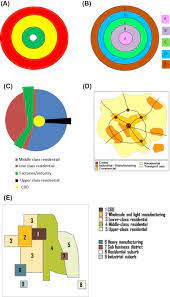
\includegraphics{fig/urban-structure.jpeg}
    \caption[Classical models of urban structure.]{There are several classical models of urban structure including Burgess' concentric zone model, Hoyt's sector model, and the multiple nuclei model described by Ullman and Harris. There's also been substantial work mapping particular patterns in particular cities. This model is more or less agnostic to the urban form, however there are interesting links and feedback loops to explore, mapping it to particular spatial forms, as discussed in Appendix~\ref{appendix-future-work} on Future Work.}
    \label{fig-urban-structure}
\end{figure}
% classical models of urban structure
% Burgess - concentric zone model
% Hoyt - sector model
% Ullman and Harris - multiple nuclei model
% and bid-rent theory
% dis-amenity as well as amenity
% SLIDES https://slideplayer.com/slide/4208853/
% http://geographylaunchpad.weebly.com/economic-activity-in-urban-areas.html
% central place theory,  - cervices and centers attract places and compete with each other. - centers have a reach, 
% measure of centrality, and surounding hinterland - the max distance to use a service, has a threshold which is who is needed. 

\section{Summary}
In this chapter we have described a very stylized models to  establish how the urban system generates rents. % and relating them to neoclassical growth theory.  
% This chapter introduces the background to the theory of the urban model. 
This is important because we will essentially build that standard urban model into our model of financialization and in the process we will be adding to the standard urban model the distributional consequences that have been overlooked, by carrying the concept of rent through to explore the distributional consequences and how the distribution of rents feeds back into the productivity of cities. 

% Our base model builds on this basic classic urban Alonso model, so it will capture core features with a simple established framework to connect with the existing literature.  One feature of this model is that none of the simplifying assumptions are essential. We maintain the basic simplicity, but the mode can easily be generalized in many ways, and there is a substantial body of work extending and varying each of the simplifications in the model, as discussed above, as well as substantial work grounding and testing the model empirically.
\chapter{Theories of Growth and Urban Scaling} 
\label{chapter-growth}

%TODO - THIS IS NOT PART OF THE BASE MODEL. CONSIDER MOVING TO THE PRODUCTIVITY SPILLOVVERS CHAPTER?
\epigraph{Cities are the engines of economic growth (Jacobs, 1969; Bairoch, 1988). It is in cities that a large share of the innovations and entrepreneurship takes place that fosters economic growth in the long run. %Spontaneous Orders and the Emergence of Economically Powerful Cities.
}{Johanna Palberg \cite{palmbergSpontaneousOrdersEmergence}}



\epigraph{If we postulate only the usual list of economic forces, cities should fly apart. The theory of production contains nothing to hold a city together.} 
% A city is simply a collection of factors of production---capital, people, and land---and land is always far cheaper outside cities than inside. Why don't capital and people move outside, combining themselves with cheaper land and thereby increasing profits?}
{Robert E. Lucas Jr. \cite{lucasMechanicsEconomicDevelopment1988}}. % is the3 atribution correct? DRR June 8

%\epigraph{Since 1980, the US economy has experienced urban-biased growth, with wages in large cities rising substantially faster than wages in smaller cities and rural areas ... 
% The left panel of Figure 1 shows average wages across US commuting zones ordered by density. 
% In 1980, workers in the cities with the highest population density (New York and Chicago) earned, on average, 34\% more than workers in cities with the lowest population density. By 2015, the gap had risen to around 62\%.}{Eckert, Ganapati and Walsh \cite{eckertUrbanBiasedGrowthMacroeconomic2022}}

% \epigraph{Hard evidence suggests that the levels of human capital in a country strongly predict its growth rates.}{Edward L. Glaeser, Cities, Information, and Economic Growth}
% \epigraph{Where are intellectual spillovers more obvious than in dense, urban environments?}{Edward L. Glaeser \cite{glaeserCitiesInformationEconomic1994}} % Cities, Information, and Economic Growth, 1994}

% \epigraph{It may be tempting to specify an aggregate production function that directly relates primary factors to final output, as is customary in much economic analysis. This standard simplification is often inadequate, however, because cities are characterized by increasing returns to scale and the way in which such increasing returns are generated has potentially important policy implications. In particular, detailed assumptions are needed about labor, the nature of products, the production function of individual firms, the input-output structure that links firms, and how firms compete.}{Spence et al. \cite{spenceUrbanizationGrowth2009}}

%, we use the Cobb-Douglas function, which is used across this entire range of literature - frame the relation of a tradition in context of  % After we develop the mathematical description of the relationship among these will discuss  in more detail, rent theory and our contribution, scaling laws, \dots  and other issues in the literature that draw on parts of this model and % ???  apply to the specific situation we're in why rent theory is related to discussions of exploitation why it might lead the inefficiencies, whether or not this links with other important models in the literature.

%``cities..% the 'force' we need to postulate account for the central role of cities in economic life is of exactly the same character as the 'external human capital'}{Robert E. Lucas Jr., \textit{ON THE MECHANICS OF ECONOMIC DEVELOPMENT (1988)}}
% ADD In this chapter we are going to xyx. This relates to space and rent in x way.
% ENORMOUS DYNAMISM OF CITIES FROM JANE JACOBS, THEN 
% Since we are looking at how financialization works to claim the urban productivity premium or value created in cities, we also need to account for how value is produced in cities, so we then introduce growth and theories of how productivity scales in the urban context.
%WHY GROWTH HERE.
%In Chapter~\ref{chapter-growth}, we integrate modern growth theory into our urban theory of rent.
%Together these pieces can be formalized as a theory of urban rent, that is a theory that captures the dominant dynamics of financialization described above.  We develop in the second part of this thesis, Part~\ref{part-model}, on the model. 
% \section{Neoclassical production theory and the city}
%\href{https://www.yourarticlelibrary.com/economics/new-theory-of-growth-of-economic-development/38329}{New Theory of Growth of Economic Development}Supriya Guru
% \section{Jacobs and the force holding a city together}
% In all of these models, the unit of analysis is the nation,  or the firm. Lucas has suggested,\footnote{Journal of Monetary Economics 22 (1988) 3-42.  ON THE MECHANICS OF ECONOMIC DEVELOPMENT*
% Robert E. LUCAS, Jr., University of Chicago, Chicago, 1L 60637, USA}
% however, that `` a national economy is a completely arbitrary unit to consider.'' and that ``we know from ordinary experience that there are group interactions that are central to individual productivity and that involve groups larger than the immediate family and smaller than the human race as a whole.''  

In Chapter~\ref{chapter-space} we described a very stylized, very standard model of the urban system to show how cities generate locational rents.
%So far, however, applications of the bid rent model have not brought forward the distributional and class features derived by the classical economists. 
The model as it stands represents a static city, however, and a fundamental feature of cities is that they grow and when they grow they produce a growing stream of value that is available for capture. %ed by their permanence and their growth over millennia. 
%
This growing stream of value is what's referred to economics as growth. If financialization is the process of capturing a stream of value for financial actors, growth is the value available for capture in cities. To understand what's at stake in cities, we therefore have to incorporate growth into our model. 
%ADD WHAT GROWTH ADDS - FIX THIS, MAKE IT MORE VIVID growth describes the mechanism by which cities create value.} 
 % It is the dynamicsm in cities. Productivity growth. } 
We're modelling how financialization captures the value created in cities. In order to show how it does this, %we need to show what it is that is being captured and it is the growth of productivity that is captured. 
including a model of growth can show how value is created and concentrated in cities. %, and the value that can be captured through land in cities through financializaiton.

%We need a mechanism of what is growing to build the model. 

%in this chapter we develop a model of how .. 
%drawing on the literature on economic growth, agglomeration effects, and the urban scaling literature. 
In this chapter we introduce two approaches to understanding the mechanism of growth. These two theories come from very distinct literatures: one from neoclassical growth theory and the other from the newer research on scaling laws. Both are supported by  substantial bodies of empirical research and they both rely  on  an overlapping set of ideas to explain their results, including notions of knowledge spillovers, network effects, and variants of specialization and human capital. 

As it turns out, they lead to a common formulation that we will incorporate into the Alonzo model described in  Chapter~\ref{chapter-space}. 
Incorporating growth will complete the urban economy model we use to test our central hypotheses about the impact of financialization in the housing market.%distribution of the urban product: that as the city grows, generating greater and greater values, much of the value appears as increased locational rents which are captured by financial capital. 
% Agglomeration is what drives the growth in the Jacobs model.

% What are the basic forces that lead to wealth: to the growth in land values and therefore to the opportunities for extracting wealth?  %What are those basic forces? 


% The order of this chapter and the order of this chapter is arbitrary. 
% I DON'T UNDERSTAND WHERE THIS QUESTION ABOUT ECONOMIC GROWTH COMES FROM, IN THE CONTEXT OF THE THESIS SO FAR,  SO i WOULD SUGGEST ADDING MORE UP FRONT SUCH AS: As we seek to understand the effects of financialization on WHAT? distribution within an urban model?? it's crucial to understand the significance of cities themselves to economic productivity. In this chapter we describe how agglomeration effects.... DO WHAT??\
% DEFINE AGGLOMERATION HERE. 
% EXTEND/CUT AND PUT HERE JACOB'S VISION OF THE DYNAMISM OF THE CITY AND HOW IT ACTUALLY CREATES VALUE
% ADD SOMETHING TO INTRODUCE  GROWTH IN ECONOMICS AND WHY IS MATTERS TO YOUR THESIS. IT"S NOT CLEAR TO ME HOW THIS COMES INTO THE PICTURE YOU"VE BEEN CAREFULLY BUILDING YET. WHAT ARE YOU ACTUALLY ADDING TO THE THEORETICAL BASIS FOR YOUR THESIS IN THIS CHAPTER AND WHY IS IT NECESSARY FOR WHAT YOU ARE DOING WITH THIS MODEL? iE WHY DOES GROWTH MATTER? 
%But what is the source of economic growth and innovation that has characterized human civilizations? 
Although they lead to essentially the same formal model at the level of generality we require for our model, %Although the models are equivalent for our purpose, 
the emphases and causal logics differ. One emphasizes processes in the industrial sector as drivers of growth, the other, associated with Jane Jacobs, emphasises mechanisms happening in cities as part of the urban system. %the nature of the urban system. 
Both arrive at an exponential model of growth, but the first comes to this through a focus on industrial and economic activity, while the second looks more at the ways cities serve to concentrate economic activity and social connections. The latter is the explanation most relevant to our work.

In The Economy of Cities, Jacobs \cite{jacobsEconomyCities1969} argued that %put forward a compelling suggestion: %Agglomeration is here mechanism: %in response to an important question in economics:  
cities are the primary drivers of economic development, and the mechanism that explains growth is the expansion of opportunities for sharing and creating ideas as population and population density increase. Jacob's argument is essentially that the density of cities produces an agglomeration effect that drives economic growth.\footnote{Glaeser et al. \cite{glaeserGrowthCities1991} refer to the Jacobs model as the Jacobs-Rosenberg-Bairoch \cite{bairochCitiesEconomicDevelopment1988, rosenbergTechnologicalChangeMachine1963} model.} %Though Jacobs is an urban theorist, her work has been 
Robert E. Lucas, one of the leading pioneers of the neoclassical growth theory, argues that the Jacobs approach explains something essential about how cities create value that is not captured in accounts that don't centre the specific advantage of urban density: % has explanatory power when applied to cities: 

\begin{quotation}
    \noindent Her emphasis on the role of cities in economic growth stems from the observation that a city, economically, is like the nucleus of an atom: If we postulate only the usual list of economic forces, cities should fly apart. \textbf{The theory of production contains nothing to hold a city together (emphasis ours)} A city is simply a collection of factors of production---capital, people, and land---and land is always far cheaper outside cities than inside. Why don't capital and people move outside, combining themselves with cheaper land and thereby increasing profits? Of course, people like to live near shopping, and shops need to be located near their customers, but circular considerations of this kind explain only shopping centers, not cities. Cities are centered on wholesale trade and primary producers, and a theory that accounts for their existence has to explain why these producers are apparently choosing high rather than low-cost modes of operation. \cite{lucasMechanicsEconomicDevelopment1988}
\end{quotation}

% As a result, ``following very closely the lead of Jane Jacobs, whose remarkable book The Economy of Cities (1969),'' 

Lucas goes on to suggest that: 
\begin{quotation} 
    \noindent ``[t]he `force' we need to postulate to account for the central role of cities in economic life is of exactly the same character as the `external human capital' I have postulated as a force to account for certain features of aggregative development.''
\end{quotation} 

\noindent He concludes that if this is so ``\textbf{\dots land rents should provide an indirect measure of this force (emphasis  ours)}'' %, in much the same way that schooling-induced earnings differentials provide a measure of the productive effects of internal human capital. 
\cite{lucasMechanicsEconomicDevelopment1988}.  

% Rent tells where the surplus is located because it represents something about this value.  Talking about rent because it is where you can measure this proximity to this urban center, that's driving growth, which is what surplus is, what is what can be captured. It is a measure of what can be captured by financialization. Why look at rent rent as a way to study financialization. rent is how


Lucas' observation is important for our work because it implies that there should be a link between the Jacobs urban mode, which is based on urban agglomeration,  the results of the neoclassical growth model operating at the level of nations, the scaling literature on cities and rent theory. 
We believe that the urban rent profile provides that link. %{\color{red} The urban rent profile is a price for proximity to value creation in the urban center. For Lucas, rent is how you can measure urban value creation in cities. This points to what's at stake when you capture rent.  You're actually capturing the value created by the whole set of processes that dynamically concentrate and grow value in cities. 
% We go on to make explore the formal identity if the neoclassical growth model and the urban scaling model.}


% This insight, which parallels ours, has not been adequately explored, in our view.  Allowing Lucas to expand on his observation about Jacobs, 
%Lucas is pointing to agglomeration economies as the force that overcomes all the reason's people have to spread out. What pulls them apart is the transportation effect. 
 %So we have to have the agglomeration effect which producesd the agglomeration effect which 
% Following his reasoning the agglomeration effect produces the circumstances that generates wealth within the model. 
%We can't model what we care about with these cities  without modeling what %drives them/what holds them together. According to Lucas it is the agglomeration effects which offset all the forces of dispersion. In this model we develop the theory to model growth and aglomeration in our urban model. % with rents.
%In this chapter, we link our basic spatial model to the scaling of urban productivity,  as Lucas seems to be suggesting, and in the process,  we will provide the foundation for our model of urban agglomeration effects.
% }




\section{Cities and the scaling literature}


% put forward agglomeration effects as at the heart of creating value in cities. 
There is another whole literature that has come to approximately the same conclusion as Jacobs and Lucas, %work emphasizing the value created in cities through agglomeration effects, 
uncovering a mass of empirical evidence that wealth scales with density and that the relationship  is a power-law distribution with a remarkably consistent scaling factor. 
 

Scaling analysis is a tool developed originally in \glspl{complex system} science to investigate how \glsdisp{extensive property}{extensive properties} of the system vary with a system's size,  or `scale.' Our particular interest is in studies linking city population and economic output, but in urban science, it's been used in many studies of the relationships between urban population size and features like urban economic output, area, growth, traffic congestion costs, and even social indicators like crime and homicide rates. These studies provide insight into how these processes are affected by the size of a city. 

The scaling literature has developed %confirmed several 
the basic result of the form: 

\begin{equation}
Y=AN^\beta.
\end{equation} 
% This defines a consistent pattern of relationship between input and output here is a consistent 
EWxponential relationships between input and output so so consistent across datasets data, that they've become known as \glspl{scaling law}. In this example, $Y$ is total value produced in a city and $N$ is city population,\footnote{We follow the common convention in the scaling literature in using $N$ for the population of the city. In the neoclassical growth literature we discuss below, $L$ stands for the working population of a nation.} $A$ is a baseline value and $\beta$ relates the \gls{extensive property} $N$ to the measure $Y$. Researchers have concluded that: 

% MAYBE ADD SOME DETAILS ON SCALING. e.g. One persistent drivign result that wealth scales with density- this is jane Jacob's result. 
% There used to be health effects and really substantial tradeoffs- short lives and disease in exchange for the density and productivity of connection. This has changed. People live longer, earn more, and have by many measures higher quality of life in urban areas. 
\begin{enumerate}
 \item socioeconomic outputs like wealth, innovation, congestion, and number of homicides per year all scale superlinearly with the size of cities ($\beta > 1$) \cite{gomez-lievanoStatisticsUrbanScaling2012}. % In addition,
% \vspace{.25cm}
 % in the appendix we show their model ends up with the same structure as ours.
 % \hspace{-1cm} 
\item the relationship appears to have applied well back into pre-history, from the smallest human communities to modern megacities, % It is not a function of any government, economic, or cultural form. It's not simply modern cities or capitalist cities. 
\item scale effects derive from the capacity of people to interact (as Jacobs suggested).
% \item This is what we see in the data. Social wealth is increasingly driven by the great cities. - The future of civilization and wealth is urban.
\end{enumerate}
These scale effects are the same as the agglomeration effects long discussed in the economics literature. Vast empirical work on scaling reveals that the super-linear scaling of wealth in cities is one of the most persistent stylized facts in economics. 

% Neoclassical production theory does not address the spatial structure of the economy. Why are there cities? What drives the historic transition from land-based agricultural society to a much denser urban society? 



\section{Agglomeration effects}
% BEGIN LEWIS STUFF, THEN MOVE INTO ECONOMIC SUPPORT
% There is a considerable 

% This is  there. it's called an agglomeration economy emprically and there's strong empirical evidence it holds strongly and a whole range of theoretical explanations. it follows these empirical results.


The history of economic thinking about agglomeration effects goes back a long ways, at least to  Alfred Marshall in 1890 \cite{giddingsPRINCIPLESECONOMICSAlfred1890}. % 
%The literature offers support for all the main building blocks of the frame- work proposed here: an upward-sloping wage curve, a cost of living that rises with city size, a bell-shaped net wage curve, and some labor mobility driven by net wage differentials. 
More recently, a large body of literature has demonstrated the existence of agglomeration economies in developed economies (see Rosenthal and Strange \cite{rosenthalEvidenceNatureSources2004} for a review). Empirical support for the framework includes \cite{spenceUrbanizationGrowth2009, durantonAreCitiesEngines2009, durantonHumanCapitalExternalities2007}. 

\begin{figure}[htb]
    \centering

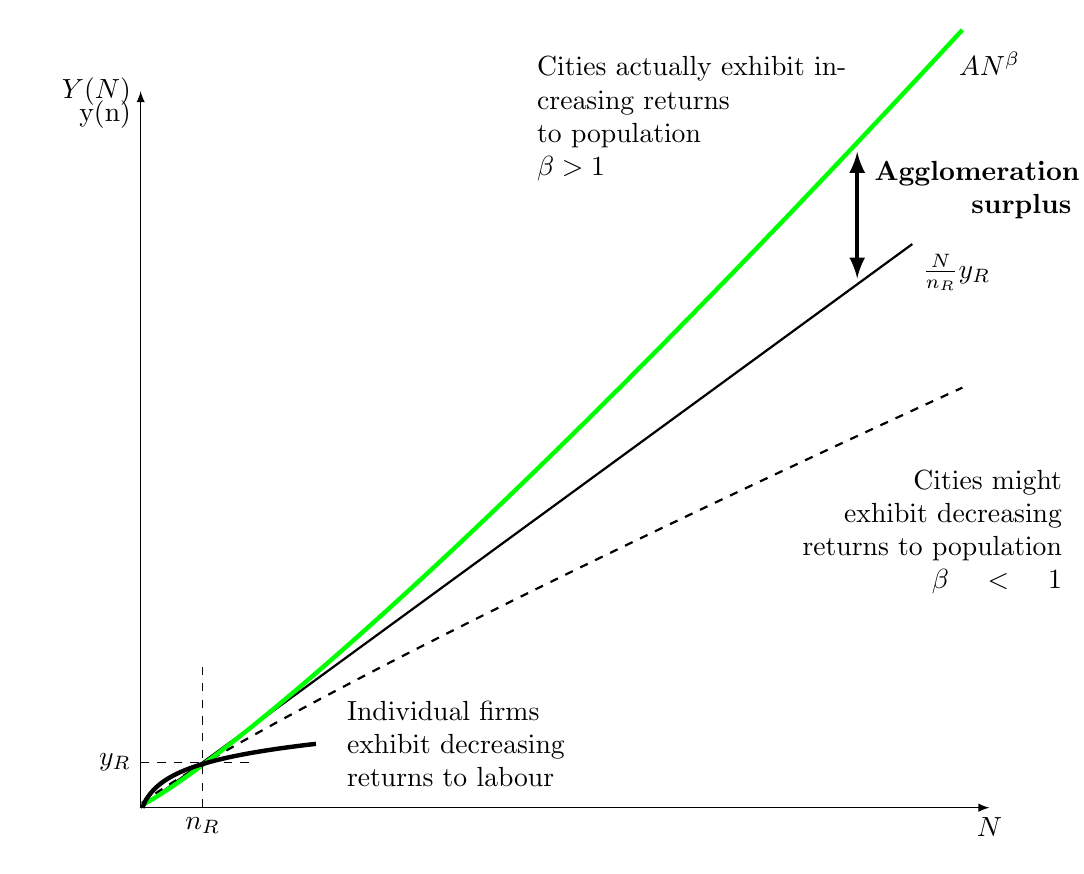
\begin{tikzpicture}[scale=.7, my plot/.style={thick, smooth, samples=100, domain=0.1:2.2},
plot2/.style={thick, smooth, samples=100, domain=0.1:14.99},
                    my grid/.style={dashed,opacity=0.5, every node/.style={black,opacity=1}},
                    my axis/.style={latex-latex}]
 
 \draw[my axis] (0,13)node[left] {$Y(N)$} --(0,0)-- (15.4, 0) node[below] {$N$}; 
%creates the axis 
 \node at (0,13)[below left]{y(n)};
 
\coordinate (origin) at (0,0);
\def\x{0.45}
\def\y{2.1}
\def\b {$15/(2*ln(\y)+.05)$};
%\def\p{0.55} % define the x, y and p )(midpointvalues
%\draw[my plot] (0,0) plot (\x,{ln(\x)});  %Draws curve
%\draw[my plot] (0,0) plot ({\x-.08},{2.3+ln(\x)}); 
\coordinate (Uy) at (\y,{2*ln(\y)+.05});

% THREE SCALE POSSIBILITIES
\draw [thick, ](0,0)--(14, 10.22583)node[below right]{$\frac{N}{n_R}y_R$};   %diagonal line CRS
\draw[plot2, dashed] (0,0) plot ({\x-.08},{(\x)^0.9/1.5 }); %DRS
\draw[plot2, ultra thick, green] (0,0) plot ({\x-.08},{(\x/1.5)^1.15});%
\node at (15.4, 13.5){$AN^\beta$};

%  TEXT
\node at (13.8,12.5) [left, text width=4.5cm]{Cities actually exhibit increasing returns\\ to population\\ $\beta>1$};%IRS
\node at (13.5,5)[text width=4.5cm, align=right] {Cities might\\ exhibit decreasing \\returns to population \\ $\beta<1$};% DRS

% ARROW
\draw[latex-latex, ultra thick] (13, 11.9)--(13, 9.6);
\node at (15.1, 11.2)[ text width=2.5cm, align=right]{\textbf{Agglomeration\\ surplus}};
%\draw[latex-latex] (13, 8.4)--(13, 9.5)node [below right, text width=1.5cm]{\textbf{$\pi$}};

\begin{scope}[ yscale=.75,xscale=1.5]% shift={(1.9,0)} ,
	\coordinate (Uy) at (\y, {2.3+ln(\y)});
  \draw[my plot,ultra thick] (0,0) plot ({\x-.08},{1.15+ln(\x)/2})node[right=.25cm, text width=3.9cm]{Individual firms\\ exhibit decreasing\\ returns to labour}; % production function for generic ferm
	\draw[dashed](.75, 0)node[below]{$n_R$} --(.75, 3.4);
    \draw[dashed](0,  1.1)node[left]{$y_R$} --(1.4,  1.1);
\end{scope}
%
%
%\begin{scope}[shift={(1.9,0)}]
%
% \def\x{0.45}\def\y{2}\def\p{0.55} % define the x, y and p )(midpointvalues
%\draw[my plot] (0,0) plot (\x,{ln(\x)});  %Draws curve
%
%\coordinate (start plot) at (0.6,{ln(0.16)}); % domain start
%\coordinate (end plot) at (10,10); % domain end
%%\draw[my axis] ([shift={(-0.5cm,0.5cm)}]start plot |- end plot) node[left] {$Y(\cdot)$} |- node[coordinate](origin){} ([shift={(0.5cm,-0.5cm)}]start plot -| end plot) node[below] {$L$}; %creates the axis a little 
%
%\coordinate (Ux) at (\x,{ln(\x)}); % set the u(x) coordinate on the curve. Not used
%\coordinate (Uy) at (\y,{ln(\y)}); % set the u(y) coordinate on the curve
%
%\draw [](origin)--(Uy)  ; 
%
%\draw[my grid] (Uy) |- node[below]{$L*$} (origin) |- node[left]{$Y^*$} cycle;%below from on curve, the 
%
%\end{scope}

\end{tikzpicture}

    \caption{While each individual firm exhibits decreasing returns to scale, the city as a whole exhibits increasing returns to scale, and thus produces an agglomeration surplus, $AN^\beta-\frac{N}{n_R}y_R$.}
    \label{fig-agglomeration-surplus} % WAS {fig:Agglomeration-surplus} i think
\end{figure}
% THE FIGURE ILLUSTRATES A GAP IN NEOCLASSICAL PRODUCTION THEORY that we aim to address with this work. THE STRAIGHT LINE IS WHAT NEOCLASSICAL PRODUCTION THEORY PREDICTED. 
 
Our treatment of the urban surplus, which is central to this thesis, is illustrated in Figure~\ref{fig-agglomeration-surplus}. 
% Figure~\ref{fig-agglomeration-surplus} illustrates the increasing returns to urban size. 
\begin{figure}[htb]
    \centering

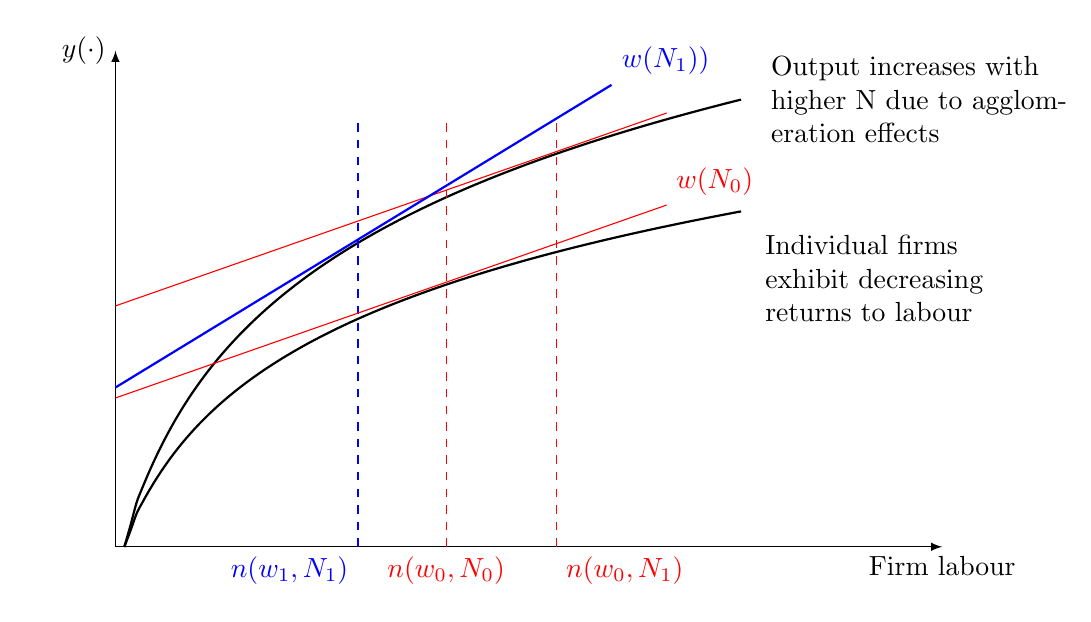
\begin{tikzpicture}[scale=.7, my plot/.style={thick, smooth, samples=100, domain=0.1:1.5},
plot2/.style={thick, smooth, samples=100, domain=0.1:9},
                    my grid/.style={dashed,opacity=0.5, every node/.style={black,opacity=1}},
                    my axis/.style={latex-latex}]
 
 \draw[my axis] (0,9)node[left] {$y(\cdot)$} --(0,0)-- (15, 0) node[below] {Firm labour}; %creates the axis a little 

\coordinate (origin) at (0,0);
\def\x{0.45}
\def\y{2.1}
\def\b {$15/(2*ln(\y)+.05)$};
\coordinate (Uy) at (\y,{2*ln(\y)+.05});


\begin{scope}[ yscale=6, xscale=8]% shift={(1.9,0)} ,
	\coordinate (Uy) at (\y, {2.3+ln(\y)});
  \draw[my plot, thick] (0,0) plot ({\x-.08},{1.15+ln(\x)/2})node[right=.25cm, text width=3.9cm]{Output\ increases\ with\ higher\  N\ due\ to\ agglomeration\  effects}; % production function for generic ferm
\draw[dashed, red](.75, 0)node[below]{$n(w_0, N_0)$} --(.75, 1.3);
\draw[dashed, thin, red](1., 0)node[below right]{$n(w_0, N_1)$} --(1.0, 1.3);
\draw[dashed, blue](.55, 0)node[below left]{$n(w_1, N_1)$} --(.55, 1.3);
\end{scope}

\begin{scope}[ yscale=4.5, xscale=8]% shift={(1.9,0)} ,
	\coordinate (Uy) at (\y, {2.3+ln(\y)});
  \draw[my plot,thick] (0,0) plot ({\x-.08},{1.15+ln(\x)/2})node[below right=.25cm, text width=3.9cm]{Individual firms\\ exhibit decreasing\\ returns to labour}; % production function for generic ferm
\end{scope}

 \draw [thin, red ](0,2.7)--(10, 6.2)node[above right]{$w(N_0)$};   %wage line
  \draw [thin, red ](0,4.37)--(10, 7.87);%node[below right]{$w(N_0)$}; 
  \draw [thick, blue](0,2.89)--(9, 8.38)node[above right]{$w(N_1))$};   %wage line

\end{tikzpicture}

    \caption{Increasing population raises the productivity of workers firm, but is only possible if the wage rises. Firm size may rise or fall}
    \label{fig-wage-workforce-effects} % WAS {fig:Agglomeration-surplus} i think
\end{figure}
% THE FIGURE ILLUSTRATES THE DOUBLE EFFECT OF  INCREASING POPULATION ON FIRM SIZE 
which illustrates how agglomerations might affect returns to scale in the aggregate.
In the lower left, we illustrate a single firm with decreasing returns (DRS) to scale operating at its optimal scale, $n$. The thick diagonal line represents the effect of increasing the number of firms operating at the optimal scale. It is the constant returns (CRS) line. If congestion effects from bringing a large number of firms together were dominant, a city would exhibit decreasing returns to scale,  $N$, and agglomeration would not occur. Research indicates that cities exhibit increasing returns to scale (IRS), illustrated by the upper line, which shows the city generating an increasing surplus as it grows. Even though there are other effects/phenomena, such as congestion as density increases that could theoretically result in cities exhibiting diminishing returns to scale, the evidence suggests that agglomeration effects dominate. The curvature of the line in Figure~\ref{fig-agglomeration-surplus} is determined by an overall  function of the form $N^\gamma$, which we will introduce into in the production function for urban firms.\footnote{The way $N$ enters the firm production function appears to be different from the way it enters the scaling law. We explore the underlying identity below.} 

The empirical \glspl{scaling law} is a feature of urban systems on average across many different contexts.  Empirical work has found %The main conclusion of this literature is the finding of 
scale economies in the range of 3--8 percent (a 10 percent increase in the size of an activity in a city raises productivity in this activity by 0.3--0.8 percent). These agglomeration effects take place both within sectors (localization economies) and between sectors (urbanization economies),  in developed and developing countries, a throughout different historical periods \cite{bettencourtIntroductionUrbanScience2021}. % The results for developing countries are usually similar,  although far less research about agglomeration economies has been conducted in such settings. 
% }
% \vspace{2cm}
 %We will show that they provide a model that can explain economic growth.% If the population rises, the output must rise more than proportionately. %, but if the population responds to the wage premium, the population should then rise. 

The effect of rising agglomeration effects for the firm in our model is ambiguous. Workers are more productive, leading firms to increase employment, but increasing the population requires a higher wage, which negatively affects employment. The result depends quite sensitively on the specific parameterization. We illustrate the two effects in Figure~\ref{fig-wage-workforce-effects}. Fortunately, for our analysis we do not need to know how much population growth goes to existing firms and how much goes to an increase in the number of firms.


\section{Neoclassical growth theories}  \label{section-growth}

Growth theory offers one of the most influential efforts to understand the wealth agglomeration effects established in the scaling and agglomeration literatures.  Growth theory originally focused on identifying the dynamics of macroeconomic systems, and in particular with the implications for the growth of national income. Early models \cite{keynesGeneralTheoryEmployment1937, harrodEssayDynamicTheory1939, domarCapitalExpansionRate1946}  employ a macroeconomic savings function which usually has a fixed savings rate, with savings being reinvested in productive capital. Later models endogenize the savings-investment process. 

The growth models, however, were not spatial models and necessarily abstracted from land rents and distribution. They have nothing to say about the distribution of city products and the effect that distribution might have on growth. When we focus on cities, however, it will become necessary to develop an analysis of city-level saving and investment. %We will do 
IN ORDER TO DO THIS WE DRAW ON SOLOW SWAN APPROACH TO FILLING A SLIGHTLY DIFFERENT GAP IN THE PRODUCTION FUNCTION.

\subsection{The Solow-Swan growth model}

In addition to not being a spatial model, urban growth theory had an important flaw. It did not completely explain the data. % {\color{red} FIX 
The approach taken to address that challenge offers parallels to how we can model urban agglomeration mechanisms.
Existing models of production had described national output as a function of two factors, the national capital and labour stocks. Output should therefore have been completely determined by the growth of those stocks and nothing else. Productivity actually grew more over time than the increases in labour and capital stocks could explain if the production function was correct.

%Solow and others realized it  wasn't working. 
In 1956 Robert Solow \cite{solowContributionTheoryEconomic1956} and Trevor Swan \cite{swanEconomicGrowthCapital1956}
addressed this gap in neoclassical production theory. Solow's paper in particular stimulated a whole literature in the 1960s and launched an entire subfield known as neoclassical growth theory.\footnote{Solow and his contemporaries, including Edward F. Denison \cite{denisonSourcesEconomicGrowth1962}, were attempting to account for the trajectory
of U.S. GDP growth, not to provide a theory of economic development as later theorists were. The distinction, although it does not seem to be commonly drawn, is between quantitative change in the level of GDP and qualitative change resulting from innovation and structural transformations.} %, exploring many variations on the original one-sector structure.  

The \gls{Cobb-Douglas} production function that was in traditional  use neoclassical production theory had been estimated by Cobb and Douglas \cite{cobbTheoryProduction1928} as early as 1928. It had the form
\begin{equation*}
Y=AK^\alpha L^\beta, 
 \label{eqn-Cobb-Douglas}    
\end{equation*}
where $L$ represented the national labour stock, $K$ the national capital stock and  $A$ a convenient scale factor. This \gls{Cobb-Douglas} form captured  important regularities in the cross-sectional national data.\footnote{The function remains the workhorse of growth theory, although later work has found models that preform better e empirically.  A 2021 meta-analysis of 3186 estimates concluded that ``the weight of evidence accumulated in the empirical literature emphatically rejects the Cobb-Douglas specification.''Gechert, Havranek, Irsova, Kolcunova (2021), ``Measuring capital-labour substitution: The importance of method choices and publication bias,'' \cite{GET_REF}. %Review of Economic Dynamics, doi:10.1016/j.red.2021.05.003, S2CID 236400765. 
More sophisticated models such as the CES and translog (TODO WHAT DOES THIS STAND FOR?) functions are now preferred for estimating production functions \cite{GET_REF}.}  % FI
% but the estimates soon showed a systematic bias with time series. 

By the early 1950s it was clear that estimated model parameters were underpredicting output when current levels of national capital and labour stocks were used. Something that was not captured in the initial model was changing over time. The obvious conclusion was that value of the the scale constant $A$  was not constant, it was time-dependent  
 \[Y=A(t)K^\alpha L^\beta.\]
Solow and Swan proposed a way to extend the standard \gls{Cobb-Douglas} production to explain rising productivity over time. 
 %offered a possible explanation for why it would be changing, opening the field for a further series of refinements in an enterprise that became known as `growth theory.' %   R.E. Lucas, Jr., On the mechanics of economic development.}
Solow  argued that ``As a result of exogenous population growth the labour force increases at a constant relative rate'' that we will represent by  $g$:
  \[L(t)= L_0e^{gt}.\] 
If we insert this term into the production function we get a scale term that depends on the changing population 
\begin{eqnarray}
Y &= AK^\alpha (L_0e^{gt})^\beta\nonumber\\
  &= A(e^{gt})^{\beta}K^\alpha L^\beta,
\label{eqn-solow-swan3}
\end{eqnarray}
we see that $A(t)$ can be written
 \[A(t)=Ce^{gt\beta}.\]
transformation provided  the time-dependent term needed to allow the model to track the data better. The model is now known as the \gls{Solow-Swan model}. 

The \gls{Solow-Swan model} correctly predicts the directions of savings and population growth, but not the magnitudes \cite{mankiwContributionEmpiricsEconomic1992}. It successfully explained a good deal of the until-then-unexplained variation over time and between nations. More than half  of the cross-country variation in income, for example,  can be explained by differences in per capita saving (capital) and population growth alone. The estimated influences of saving and population growth with the Solow model appear too large, however. To understand the relationship between saving, population growth, and income, it was necessary to go beyond the  Solow-Swan model.

In the Solow-Swan model growth in productivity is exogenous. By treating economic expansion as exogenously driven, neoclassical growth theory did not explain % could not focus on 
the underlying forces which determine long-run development of nations.   Robert E. Lucas \cite{lucasMechanicsEconomicDevelopment1988} would observe that \begin{quotation}
``[i]t seems to be universally agreed that the model \dots is not a theory of economic development.   \dots while it is not exactly wrong to describe these differences (in GDP  growth rates) by an exogenous, exponential term like A(t), neither is it useful to do so. We want a formalism that leads us to think about individual decisions to acquire knowledge and about the consequences of these decisions for productivity.'' \end{quotation}


The models that followed Solow-Swan, starting with Arrow's 1962 model of `learning by doing' \cite{arrowEconomicImplicationsLearning1962a}, introduced \gls{human capital} and learning in a variety of ways, thus `endogenizing' the growth  process. %This is a central insight. 
This is an important extension. 

Human capital may enter the model as a stock of experience that accumulates in the firm or the sector. It may be proxied by aggregate prior capital investment, as in Arrow's model. The scale term $A$ then becomes $A(K)$.\footnote{The use of capital as the limiting factor formally resembles the Harrod-Domar model \cite{harrodEssayDynamicTheory1939, domarCapitalExpansionRate1946}, although the interpretation is different. Arrow uses capital a a proxy for knowledge, not machinery.} Arrow uses a dynamic interpretation of increasing returns approach  that was perhaps the first to  render technological progress endogenous in a growth model.\footnote{The version of how the field has developed that we present leaves out many who were engaged in and contributing to the evolution of growth theory. The introduction to  Arrow's paper cites several. Spear and Young \cite{spearMACROECONOMICDYNAMICSSURVEY2018} provide a more inclusive overview. It seems clear that neoclassical growth theory was the result of a general ferment in the economic profession, not simply the product of a few pioneering individuals.} 
% {\color{red} 
% and  Levhari  \cite{levhariExtensionsArrowLearning1966} by  the experience of workers,  as in Sheshinski \cite{sheshinskiOptimalAccumulationLearning1967}.
% } 
Other proxies for learning were considered by various authors \cite{levhariExtensionsArrowLearning1966, sheshinskiOptimalAccumulationLearning1967}, incuding the the amount of innovation by other firms and sectors  \cite{kingEndogenousGrowthRole1989}. Sheshinski and Levhari showed that Arrow's formulations was quite general and could incorporate a range of effects as well as different forms for the production function.


To understand  growth theories based on \gls{human capital},  sometimes called `\gls{effective labour},' it is helpful to notice that Solow's formulation is unchanged if we substitute `labour $\times$ skill' for $L$ in his model. Both components of `labour $\times$  skill,' or effective labour grow over time. Output then grows at the same rate as the effective labour supply. Mankiw, Romer and Weil \cite{mankiwContributionEmpiricsEconomic1992} showed that  
Solow's model  augmented by including human capital $H$  fit the data better the unamended Solow-Swan model. Their equation was, in our notation,   
\begin{equation*}
Y=A(t)K^\alpha H^\gamma L^\beta, 
% \label{eqn-mankiw}    
\end{equation*}
where $H^\gamma$ is a form of human capital. (They assume $\alpha+\gamma<1$, which implies decreasing returns to all forms of capital take together.) The apparent effect of increasing labour supply and technological change could be, therefore, the combined effect of rising labour supply, technological change, and increasing labour skill and even agglomeration. Later studies would attempt to disentangle the four components.


%???       It is no surprise that adding a variable allowed the model to track the data better. More  interesting is that the appearance of term $1-\alpha}$ in the scale factor $A$ suggests a spillover effect of human capital on the productivity of other factors.\footnote{Breton, T. R. (2013). ``Were Mankiw, Romer, and Weil Right? A Reconciliation of the Micro and Macro Effects of Schooling on Income'' (PDF). Macroeconomic Dynamics. 17 (5): 1023--1054. doi:10.1017/S1365100511000824. hdl:10784/578. S2CID 154355849.}  

%The estimated model explained 78\% of the variation in income across countries.
% the estimates of $\beta$ implied that\textbf{ human capital's external effects on national income are greater than its direct effect on workers' salaries.}%(\url{https://en.wikipedia.org/wiki/Solow\%E2\%80\%93Swan_model)}.  Theodore Breton provided an insight that reconciled the large effect of human capital from schooling in the Mankiw, Romer, and Weil model with the smaller effect of schooling on workers' salaries. He demonstrated that the mathematical properties of the model include significant external effects between the factors of production because human capital and physical capital are multiplicative factors of production.[20] The external effect of human capital on the productivity of physical capital is evident in the marginal product of physical capital:
%    \[ MPK={\frac {\partial Y}{\partial K}}=\frac {\alpha A^{1-\alpha }(H/L)^{\beta }}{(K/L)^{1-\alpha} }\]

 %Ludcas on the mechanics of ec dev

%, We draw on these models,  formulated at the level of nations, to describe  agglomeration and productivity at the level of cities.% (per Lucas on mechanics), See Burmeister and Dobell (1970) for an excellent introduction and survey. 

%In these models, saving and population growth rates determine the growth trend of the economy. which assumed  diminishing returns to capital and labour separately and constant returns to both factors jointly, 

% MISSED Mankiw et al.equation 
 % The  model became\footnote{Because they work with time series, all the quantities are dated. We omit the time marker for notational simplicity.}

% NOTE for  K   
%If we replace the labour-capital technology of the Solow model with a land-labour technology of the same form, and treat labour as the mobile factor and land as the immobile, we obtain a model that predicts exactly the immigration flows that occurred and for exactly the reason - factor price differentials - that motivated these historical flows

%One of the predictions of the neoclassical growth model, even  when the concept of capital includes human capital, is that without  continuing improvements in technology, per capita income growth eventually ceases on the equilibrium path. 

Identifying  plausible ways that human capital might affect development was relatively easy. However, measurement of human capital presents great practical difficulties. To extract the implications of a particular path, it was also necessary to construct a tractable model, analyze its dynamic properties, and find proxy data to test the initial hypothesis.   A series of papers did exactly that. It is important to note that these models all open the possibility that governments can promote growth through investment in education, research, technology transfer, and incentives for firms.

%{\color{red} In this work, human capital comes in in xx way. --. we integrate parts of these models.. this is what we take from this work..}


%{\color{red} WE STOPPED HERE} 

\subsection{Endogenous (neoclassical) growth models}
A new wave of research on economic growth was stimulated by Romer \cite{romerIncreasingReturnsLongrun1986} and Lucas \cite{lucasMechanicsEconomicDevelopment1988}. In their models, returns to scale are external to single economic agents and internal to a sector or larger parts of the economy. In other words, private decisions by firms or individuals may enhance the productivity of other firms or individuals. This insight is built into our urban models as a growth-enhancing effect of agglomeration. 

%Basically, two branches have developed, pioneered by Romer (1990) and Lucas (1988). CHECK THESE SOURCES

Paul Romer's 1986 model, based on his 1983 thesis \cite{GET_REF}, describes `learning by investment.' In this model, the increase in {total factor productivity} depends on firms' learning, or investment specifically in knowledge accumulation through research, rather than output. He goes on to  explicitly model the decision to invest in the production of knowledge. The production function  can be written
\[Y = A(R^T)R^\gamma  K^\alpha L^\beta, \]
where $R$ is the research effort of the specific firm, and $R^T=\sum_iR_i$ is the total research in the industry,  $R$ is a choice variable for the firm, which is to say, it decides how much to invest in research. The distinctive  feature of this model is the spillover effect on all other firms of the firm's R\&D investment. Economy-wide or  \gls{total factor productivity} is enhanced by individual firms investing in their own productivity. $A(R^T)$. %\textbf{This is the logic of our own model of agglomeration effects in the city.}

In 1988 Lucas also argued that technical progress is endogenous. He proposed a model that is  close technically to the models of Arrow (1962), Uzawa (1965)and Romer (1986). Following our notation, 
\[ Y = A(H^e) K^\alpha (HeL)^\beta \] 
where $H^e$ is the economy's average level of skill (human capital).  Improvements in skill in any firm  increase overall productivity. The compound term, $HeL$,  can be understood as the `effective' labour force of the firm, where $L$ is size of the workforce, $H$ is the skill level of the  workers that the firm hires,  $1-e$ is the fraction of worker time  spent in training, and $e$, is the fraction of work time spent working.\footnote{A feature of this formulation is that $e$ is a choice variable for the firm. It could as easily be a choice variable for workers in the aggregate model.} 
More time training increase $H$ but reduces $e$, so the firm faces a tradeoff between investing time in training and working in firms.
% CHECK NOTATION ***

The difference between Romer style and Lucas style theories is that endogenous growth in the theory of Romer is caused by accumulating technology (or knowledge), which can be called social capital, while in Lucas it is through training, which increases human capital. %\footnote{Although it is not of direct concern for our work, it is useful to recognize that much of the emphasis in these models is on finding the conditions that can explain the observed long-term  and growth over and above that driven by exogenous population or technology growth. } 
Although Romer emphasizes the decisions made by firms while Lucas bases his theory mainly on  decisions by households, both illustrate internal effects of human capital. In one case it whether it is an external or `spillover' increasing the productivity of all firms, in the other it is the individual worker undergoing training to become more productive. 

The evidence supports the existence of significant learning spillovers in a variety of industries. Using survey data, Mansfield (1985) found that information about new processes and products in ten industries surveyed had widely diffused within a year. Spillovers have also been found in econometric studies: Irwin and Klenow (1994) find them in semiconductors; Thornton and Thompson (2001) in wartime shipbuilding; Lieberman (1989) in chemicals; Foster and Rosenzweig (1995) in the adoption of high-yielding seed varieties; and Conley and Udry (2007) in the adoption of best practices by Ghanaian pineapple farmers.\footnote{A model of a national economy that uses the number of urban dwellers would probably track output just as well as one using the number employed as the mainline growth models do. As countries develop, cities account for an ever-increasing share of  national populations and an ever-increasing share of national income.  This is  even more likely when we recall that the principle insights coming out of neoclassical growth theory point to human capital and education as the mystery factor in growth and cities are where the most skilled workers concentrate and where the strongest educational institutions tend to be.} 


\section{Jacobs-style agglomeration effects and the scaling law}\label{section-growth-Jacobs}

Jane Jacobs' work, mentioned above, formulates % introduced 
an alternative but compatible explanation for the increasing productivity that growth theorists tried to explain. She argued that when people come together in cities they make each other more productive \cite{jacobsEconomyCities1969}. In her view the increase in productivity is a result of increasing communication and other network effects between people. % This is a theory of urban agglomeration that can be written for the firm level as%, Remaining with the notation of the growth theorists, it can  be written, 
If we take the relationship implicit in her work, and write it in the language of modern growth theory, we get:

\begin{equation}
y(t) = A_f(L^T,t) K^\alpha L^\beta 
%y(t) = A_f(L^T(t)) K(t)^\alpha L(t)^\beta, 
\label{eqn-production-jacobs}
\end{equation}
where the  lowercase $y$  indicates that Equation~\ref{eqn-production-jacobs} is a \textbf{firm-level}, or micro-economic, formulation. The $L^T$  in the function $A_f$ gives the size of the total urban labour force or urban population.

We impose the standard neoclassical diminishing returns to scale\footnote{$Y(\delta K,\delta L< \delta Y(K,L)$.} assumption on the \gls{Cobb-Douglas} production function, i.e. that 
$\alpha +\beta <1$.  
 %The Cobb-Douglas function used to illustrate these models has the required property.\footnote{To see why, notice that $A(\delta K)^\alpha (\delta L)^\beta = A\delta^(\alpha+\beta) K^\alpha L^\beta$, and $\delta^(\alpha+\beta) <\delta$ for $\delta>1$. } 
 If we then sum across all $F$ firms and assume that all firms are identical we get the \textbf{aggregate} urban production function
\begin{equation}
Y(t) = A(L^T, t)* F *K^\alpha L^\beta. 
\label{eqn-production-jacobs-agg}
\end{equation}
% At the level of the city the aggregate output for this model can be written
% \begin{equation}
% Y(t) = Y_c(L^T(t), t) 
% \label{eqn-production-jacobs-city}
% \end{equation}

If we use consider a fixed capital-labour ratio $d$ as Arrow does,  capital used by the firm is  $K=d*L$ and Equation~\ref{eqn-production-jacobs-agg} becomes
\begin{align}
Y &= A(L^T, t) F d^\alpha L^\alpha L^\beta) \nonumber\\
&=A(L^T, t)F d^\alpha L^{\alpha +\beta} \nonumber\\
&= A(L^T, t) F^{1-\alpha -\beta}d^\alpha * (F L)^{\alpha +\beta} \nonumber \\
&=\bar A(L^T, t) (L^T)^{\alpha +\beta},  
 \label{eqn-production-jacobs-city-2}
\end{align} 
where the  multiplicative constants,  $F^{1-\alpha -\beta}d^\alpha$, are incorporated into the scale factor $\bar A$. 

If we now specify $\bar A$ in Equation~\ref{eqn-production-jacobs-city-2} by: \begin{enumerate}
    \item   assuming that the term $L^T$ enters $\bar A(L^T, t)$ exponentially as in the scaling literature, say as $LT^\delta$,  
    \item defining $Y_0=F K(0)^\alpha L(0)^\beta$, and 
    \item allowing  for additional time dependent growth, $e^{g*t}$,
\end{enumerate}
we can write Equation~\ref{eqn-production-jacobs-city-2} 
\begin{equation}Y_c = Y_0e^{g*t}(L^T)^\gamma. \label{eqn-production-jacobs-scale}
\end{equation}
This is the model commonly used in the scaling literature. We use it as the base for our market model. 



\begin{table}[htb]\small
\centering
\begin{tabular}{|p{1.5cm}|l|l|p{1.5cm}|p{1.4cm}|p{1.cm}|l|p{2.5cm}|}\hline
\textbf{Social Rates} & \textbf{Exponent} & \textbf{Error} & \textbf{Nation} & \textbf{Obser-vations} & \textbf{Year} & \textbf{Unit} & \textbf{Reference} \\ \hline   
GDP             & 1.13 & [1.11, 1.15]  & US           & 363 & 2006        & MSA  & Bettencourt (2013)                 \\ \hline
GDP             & 1.17 & [1.11, 1.22]  & EU           & 102 &             & MA   & Bettencourt  \& Lobo        (2016) \\ \hline
GDP             & 1.22 & [1.17, 1.27]  & China        & 293 & 1996-2014   & prefectural & Zund  \& Bettencourt (2019) \\ \hline
GDP             & 1.14 & [0.98, 1.30]  & India        & 22  & 2011        & UAs  & Sahasranaman \& Bettencourt (2019) \\ \hline
Personal income & 1.1  & [1.03, 1.20]  & Brazil       & 39  & 2010        & MAs  & Breisford et al.  (2017)           \\ \hline
Personal income & 1.35 & [1.19, 1.53]  & South Africa & 8   & 2001        & MMs  & Breisford et al.  (2017)           \\ \hline
\end{tabular}
\caption[Observed scaling exponents]{Observed scaling exponents for urban systems around the world} \label{table-scaling-exponents} (source: Bettencourt \cite{bettencourtIntroductionUrbanScience2021} table 3.1)

\end{table}


To achieve increasing returns at the urban level, it is necessary that the exponents not exceed one, $\gamma=\alpha+ \beta + \delta > 1$.  Empirical  estimates summarized in Table~\ref{table-scaling-exponents} show that this condition is satisfied. These estimates provide a plausible parameter range for modelling. 

%The  model is observationally nearly equivalent to the Arrow model.

% \begin{figure}[!tb]
% \begin{center}
% 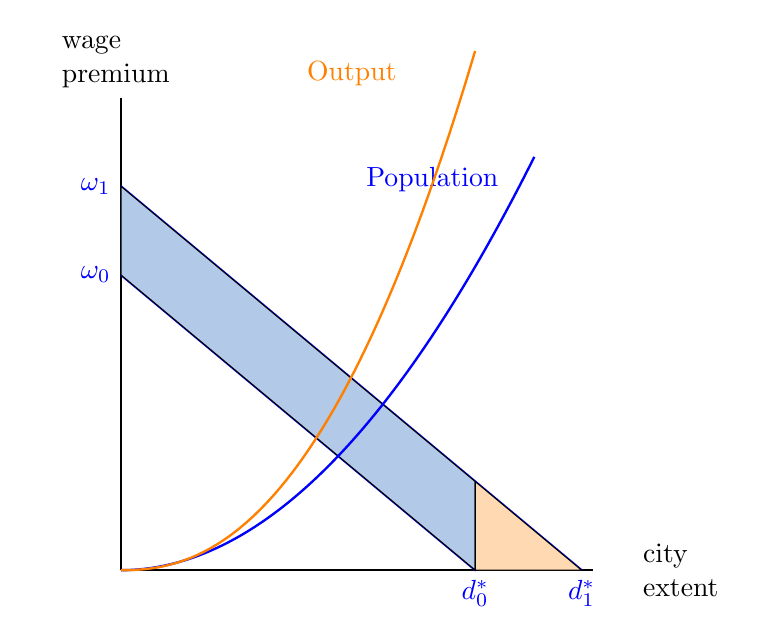
\begin{tikzpicture}[scale=.75]
\def\bndmax{8} 
\tikzset{func/.style={color=blue!80}}	
% EXTENT  BEFORE
\draw[thick](0,0)--(0,8)node[above, text width=1.5cm]{wage \newline premium}; % Y axis
\draw[thick](0,0)--(8,0)node[right=.5, text width=1.5cm]{city\newline extent};  % X axis
%\node at (3.5,-.7){Extent: Walkers};
\draw[thick, blue](0,5)node[left]{$\omega_0$}--(6,0)node[below]{$d^*_0$};
\draw[ thick, blue](0,{5*1.3})node[left]{$\omega_1$}--({6*1.3},0)node[below]{$d^*_1$};
\draw[fill=green!30!blue!30](0,5)--(0,{5*1.3})--(6,5*0.3)--(6,0)--cycle;
\draw[fill=orange!30]({6*1.3},0)--(6,5*0.3)--(6,0)--cycle;
\draw[func, domain=0:7, line width=.3mm,blue, text width=2cm] plot [samples=200] (\x,{\x^2/7})node[below left]{Population};
\draw[func,  domain=0:6, line width=.3mm, orange, text width=2cm] plot [samples=200] (\x,{\x^2.3/7})node[below left]{Output};
%\node[circle,draw=black, fill=white, inner sep=3pt,minimum size=10pt] (b) at (1,2.5) {1};
\end{tikzpicture}
% \end{center}
% \caption[Rising wage and increasing city size]{Rising wage and increasing city size. Agglomeration effects increases the wage premium from $\omega_0$ to $\omega_1$, a higher wage attracts more people to the city, leading to city growth from $d_0^*$ to $d_1^*$, which then begins another cycle of agglomeration and growth }
% \label{fig-rising-wages}
% \end{figure}
% 
\subsection{Dynamics of the Alonzo model with Jacobs agglomeration}
The increase in productivity at the firm level due to agglomeration is the force that drives the formation and growth of cities. In our model, the agglomeration-driven increases in productivity result in an \gls{urban wage premium}. The urban wage premium attracts workers to the city and pays their transportation costs. The size of the wage premium determines the size of the city.

The urban economy modeled this way provides the foundation for our analysis of the urban housing market. We are not attempting to explain the specific process that gives rise to the wage premium: there is strong empirical evidence that it exists, and it is theoretically consistent with the explanations of the growth theories described above. We do need to point to how these agglomeration effects feed into the dynamics of the housing market.

% We do not specify that make urban labour more productive than non-urban labour. % The process has deep historical roots and we do not need to provide an origin story for our project. 
%{\color{red}We can use Figure~\ref{fig-rising-wages} to emphasize the self-reinforcing nature of the mechanism. The blue line  shows population rising as the city boundary moves outward and the orange line shows productivity rising even more quickly due to agglomeration effects. Starting with a city that has grown to size $d_0^*$ based on a wage premium $\omega_0$ in Figure~\ref{fig-rising-wages}, an increase in the productivity due to the various spillover effects discussed in the literature eventually is passed through, at least in part, to the wage raising it to $\omega_1$. }

Conventional microeconomic theory provides us with a rough sketch of the complex process that must occur as agglomeration effects grow. The process will generally be slow, variable, and may involve multiple unsynchronized lags. The basic process, however, is that a firm, discovering its workers are more productive than expected, enjoys unexpected output and profits. Unexpected profits in existing firms will lead to new firms entering the industry. Since the marginal product of each worker is higher than expected, existing firms will want to hire more workers. To do so in a city with full employment, they must raise their wage offers.   The increased wage attracts workers from other firms, putting pressure on them to also increase their wage, so wages rise across the city. The general increase in the wage attracts more workers to the city.

The increase in population will eventually generate additional agglomeration benefits, further increasing wages. At the aggregate level, this positive feedback appears to be solidly supported, but locally, within firms and between firms there will be long and variable lags. Analytical equilibrium models seek to bypass these messy processes, while agent-based models attempt to incorporate them.



%The increase in wages appears as a benefit to workers as workers already in the city. %In Figure~\ref{fig-rising-wages} the area in blue-green represents the worker's share of the increased productivity of the city. 
Assuming that marginal land use per new resident is constant, the city diameter will eventually expand in proportion to the increase in the wage. %, shown as the distance $d^*_0--d^*_1$. Aggregate rent  further expands by the area shown in orange. 
Population increases in proportion to the square of the increase in diameter. %, as  the blue line shows, bu output increases proportionally, as indicated by  the orange line. 

In our model, we connect this agglomeration with financialization through the housing market. The mechanism is that increased wage is translated, with further lags, into rising home prices across the city and rising rental prices for tenants. This means that landowners capture some of the gains due to agglomeration. Owner-occupiers retain the gain and eventually realize it as increased  property values. Financialized owners claim it as rents, and can charge higher rental rates when there is more value to living in the city because of agglomeration effects. % Tenants eventually see the wage gain converted into higher rent payments. 
This flow takes the value created in cities through any mechanism of agglomeration, and captures the flow for finance. 
% Higher home prices and rental rates would be expected to lead to expansion of the housing stock. Adding to the housing stock is a slow process, however, introducing complexities including potentially complex stock and stock-price dynamics. % which we ignore.


% Jacob's view  that rising productivity as a result of urban agglomeration is consistent with the relatively recent research on urban scaling \cite{bettencourtGrowthInnovationScaling2007, loboUrbanScalingProduction2013, bettencourtIntroductionUrbanScience2021, bettencourtOriginsScalingCities2013, kaufmannScalingUrbanAmenities2022, gomez-lievanoStatisticsUrbanScaling2012}.  In section, we show that the firm-level version of Jacobs-style agglomeration in Equation~\ref{eqn-production-jacobs}  
% is equivalent to a \gls{scaling law}. This observation  links the micro-foundation of our model to the macro-economic estimates in the scaling literature. 

% The Jacobs model as we describe it at the level of the firm is 

% The Scaling literature uses  
% \begin{equation}
%     Y=A N^\gamma
% \end{equation}
%This is the function that has been estimated in the scaling literature. 
% The model commonly used in the scaling literature is 
% \[Y = Y_0e^{g*t}N^\gamma\]
% where $Y_0$ is an initial value and $g$ is an exogenous growth rate and $N$ is urban population, which is $L^T$ in our model. The key difference we need to account for is the absence of the firm level of capital and labour in the aggregate function.  %\footnote{Bettancourt (2021) writes the model \[Y_i = Y_0(t)N_i(t)^\beta e^{\xi(t)}\]. Notice that this is similar to the  form that we saw in the \gls{Solow-Swan model} if we substitute $N^\beta$ for Solow's $K^\alpha L^\beta$.  The interpretation is different because the model is used to estimate the parameter $\beta$ and $e^{n(t)}$ is described  as an error term of the form commonly used in estimating multiplicative time-series models.} 


%To show that  Equation~\ref{eqn-production-jacobs} is equivalent to a scaling law we need to  make the synergies that Jacobs points to explicit: we require $L^T$ to generate a spillover effect similar to those  identified in neoclassical growth theory. 
% There are three obvious generic ways to introduce such a term: $L^T$ can augment $A$, $K$, or $L$,

% \begin{align}
%   Y &=\left\{
%     \begin{array}{l}
%      \mathbf{\color{red}(A*L^T)}\quad K^\alpha L^\beta\\
%      A \quad\mathbf{\color{red}(L^T*K)^\alpha} \quad L^\beta\\
%     A K^\alpha \quad \mathbf{\color{red}(L^T* L)^\beta}
%     \end{array}  
%    \right\} \nonumber\\
% \end{align} 
% Each of these produces a firm-level function 
% \begin{equation}%\label{eq-JacobsCobbDouglas}
%  Y=  A(L^T)K^\alpha L^\beta 
% \end{equation}
% \[Y = A*N^\gamma K^\alpha N^\beta= AK^\alpha N^{\beta+\gamma}\]
% \[Y = A (N^\gamma* K)^\alpha  N^\beta= AK^\alpha N^{\beta+\gamma^\alpha}\]
% \[Y = A K^\alpha (N^\gamma* N)^\beta= AK^\alpha N^{\beta+\gamma}\]
% Where $\phi=\beta +\gamma$ or $\beta +\gamma^\alpha$, depending on how the spillover enters. Each of these yields an exponent on $L^T$ that may be greater than one, consistent with both Jacobs and neoclassical growth theory.

% \footnote{It differs from the Solow model in Equation~\ref{eqn-solow-swan3} Where

% \[Y = AK^\alpha \mathbf{\color{red}(L_0e^{g*t})^\beta}L^\beta\nonumber\]
% in that Jacobs, consistent with later literature, assumes that $N$ is endogenous, while Solow assumed an explicit and autonomous time-dependency of $L$.} 

%One more step is needed to produce the standard scaling law: K must be rewritten as a function of employment $N$. The easiest way is to assume as Arrow did that the production process is characterized by fixed coefficients.\footnote{With a Cobb-Douglas function  $K$ will be chosen in a fixed proportion to $L$ at any given wage-capital cost ratio.} $K^\alpha$ is then $cN^\alpha$ for some $c$. Equation~\ref {eq-JacobsCobbDouglas} becomes 



% WHERE TO PUT THIS? \cite{arvidssonUrbanScalingLaws2023} find that cities' tails are responsible for 36--80\% of the observed superlinearities across indicators. 

%will raise the wage, attracting more workers. If they are added in suburbs at the edge of the city (Ricardo's extensive margin) virtually all of the wage premium they receive is dissipated in transportation costs. Closer to the centre,  land rents rise. Owner-occupiers capture the increase as property value appreciation. Tenants are likely to be faced with higher rents.      

%If agglomeration is the source of productivity gains, however, the new workers increase the urban premium, further increasing land values and attracting more workers. 

%The rural population consists of uniformly distributed efficient mix of rural capital producers and workers, all of whom receive $\omega$.%\footnote{This does nothing but fix the price of produced capital in terms of the rural wage.} 

 %Owners of urban firms are  conventional  capitalists, who may earn excess profit if they can capture an unearned surplus from labour.  Any unearned surplus increases the return to urban capital relative to rural capital, resulting in continual expansion of the urban economy. Continuous growth in turn results in continuously rising urban land prices and hence housing costs. We ignore the distributional implications of this feature of the model, and focus instead on the part of value produced by the city that appears as land rent. 

\section{Summary}
% These distinct approaches to understanding agglomeration effects 
% (growth theory  and agglomeration approaches-- which apeare  to be fundamentally different actually produce the same quation, .--)
% We worked through derivations to show how one can be turned into the other. 
% WHENEVER TALKS ABOUT ONE - LOOKS - WHENEVER DIFFERENT INTITIAL POINT AND COME FROM DIFFERENT PLACES the growth  theory all comes out of looking at gdp growth and using the Cobb Douglass to use gdp growth.
% The agglomeration results come out of straight empirical hacking. when xyz and bettencourt go back to how you could get this equation they go back to the Cobb Douglass and that same analysis. -- that's  the logic of that whole chapter one can be turned into the other.

Growth theory, the agglomeration effects identified in Jane Jacob's work, and urban science's empirical work on scaling all produce the same equation. They come from different traditions, draw on different datasets and use different methodologies, but they get to the same place. 
 % all this relationship on why we get growing productivity and it comes to  a certain relationship
In all cases, the reason super-linear scaling of productivity in cities is that the conditions in cities make people more productive. %in cities. The relationship seems to say it's human capital not just the number of workers. %Its their productivity. 
Cities bring people together where they can specialize, get more education, and learn from another. These are all essentially agglomeration effects. 

Agglomeration effects are the third piece needed to build a model relating urban productivity and the financialization of the the urban housing market. % lucas saying - you knowo what jacobs was probably right, that's probably what we've come to with all this work (Lucas is a big  name.)
% Given that there is such a strong theoretical and empirical grounding for urban agglomeration effects in the city, 
We build our model of the housing market on top of a model of the urban system that exhibits positive agglomeration effects.  %***E EDIT THIS. TO CLARIFY RELATIONSHIP BETWEEN SENTENCES. BUILD AGGLOM EFECT INTO MODEL BY EMBEDING SCALING LAW? OR SPECIFICALLY WE EMBED??? 
We model the agglomeration effects by embedding an urban \gls{scaling law} to model how value is create in cities. %to develop the theoretical grounds of our model, we 
% and draw on neoclassical growth theory to explain the growth of national output.
The value created by the scaling effects are the value that financial actors can capture through the financialization of the housing market.

\part{Model and Analysis} \label{part-model}
\chapter{Model}  \label{chapter-model}
\epigraph{One of the very important components in the urban and agricultural land use model is the so-called \gls{bid-rent curve}. Regional and urban economists, city planners, and economic geographers have used this curve extensively as an analytical device.}{Yeung-Nan Shieh \cite{shiehWilhelmLaunhardtBidRent2004}}

% FUTURE WORK Because our goal is to extend the current model by introducing speculative motives and financialization, we retain the single-type household of the basic model, we defer the question of the differential effect on household types for later work.  

%because a key feature of this model is that it formally captures how finalization works to capture the 
%financialization is aimed at capturing the 
%rents generated by growth and specifically urban growth..

% LINK WHAT TO WHAT..
% The feature of the model that provides the necessary link is known as the `\gls{bid-rent curve}.' We will incorporate the financial sector into the land market using the bid-rent curve.

%We begin in Section~\ref{section-financialize} with a definition of the act of financializing transactions and markets,  and discuss some significant examples. 

%Finally, in  Section~\ref{section-system} we explain how financialization might affect the housing market as a system and some consequences for society in general. 
%At that point we can introduce our specific hypotheses and how we intend to test them.
% We focused on modeling the effects of financialization on and through the urban housing market to \textbf{WHY?}. 
% This is where the ghttps://www.facebook.com/profile.php?id=100000594429550eneral process of financialization At that point we can introduce our specific hypotheses and how we intend to test them.
% We therefore begin with a narrow and strict definition of the act of finacializing, followed by an explanation and examples. We then go on to explain how the term is applied at the level of systems and while markets.
% At that point we can introduce our specific hypotheses and how we intend to test them.

% COULD CALL THIS THEORETICAL DEVELOPMENT OF THE MODEL AND MAKE A SEPERATE IMPLEMENTATION CHAPTER

% This chapter describes the specific formulations % (**E USE A MORE SPECIFIC WORD THAN LINKS) % #E BUILD A PCITURE OF HOW THE MODEL DRAWS THESE TOGETHER \dots LIKE IT TAKES THESE THREAD (LIST THEM) AND COMBINES THEM INTO A MODEL THAT EXPLORE \dots USE THIS PARRARAPH TO DESCRIBE THE EXACT INTERCONNECTIONS

% the theoretical discussions of the previous chapters with an agent-based simulation model. 

% At the heart of the model is a real estate mark et in which owners, tenants, new entrants to the city and non-resident investors participate. To do that we build up our model in a series of steps beginning with a notion of economic value, adding potential speculative gains, and finally describing a transaction process. %We need to specify the market process in more detail. (???) % i DONT UNDERSTAND IF YOU ARE SAYING YOU NEED THIS? THE MODEL FILLS THIS GAP?? OR THIS IS AFILLER SENTECEN??? 

% This chapter introduce the urban spatial model and labour supply, models the production function with urban scaling of agglomeration effects with density, then introduces a model of financial investment/speculation into a spatially explicit land market model, then calculates profit, considers who gets the profit, and draws conclusions. 



%     MOVE THIS?
%Recent urban models %, on the other hand, tend to focus on the locational implications of land and transportation costs on the location of people. Wealth distribution is  often ignored. 

% - need to  model production, specifically the rising production with density. 
%There is an extensive formal apparatus in economics for considering the relation of production and output. 

% \section{The general structure of the model}
In this thesis  we describe an agent-based spatial model of an urban housing market that includes a production function modelling how urban regions generate wealth and an explicitly financialized housing market.  Where previous chapters %***E EDIT: DISCUSSED IN GENERAL THE PRINCIPLES OR DISCUSSED THE ENERAL PRONICPLES 
discussed the general principles that underlie our theoretical model, this chapter presents details about the how the variables in the computational model are defined. %Where, for example, we talk about expected price in Chapter~\ref{ch_financialization}, here we  provide the formula we use in our simulations.

% The model is introduced in the following sections:
% \begin{enumerate}
% \item In Section~\ref{sec_model_blocks} we  begin by describing the major blocks of the model. 

% \item In Section~\ref{sec_model_dynamics}  we make some comments on the dynamic properties of the model we have constructed. 

% \item In Section~\ref{sec_model_variables} we describe how a series of key  variables are constructed. The variables enter the decision-making process of agents in the market. 

% \item In Section~\ref{sec_model_bid_price}     

% \item In Section~\ref{sec_model_bargaining}    

% \item The treatment of time a periods and discounting is discussed in Section~\ref{sec_model_time}. 
%  Section~\ref{sec_model_price_expectataions}


% \item In Subsection~\ref{sec:Production-fn} we introduce the production function, introduce the labour supply and the urban model, the source of the surplus,  then we calculate profit, consider who gets the profit, and from there we draw our conclusions.. then we calculate the urban surplus, and consider who gets it. 

% \item Appendix~\ref{appendix-model-implementation} gives more details, describing the calculations, and showing how the model is implemented in code. 

% \end{enumerate}

% % % In subsequent sections  .. (Derivation details in Section~\ref{section-derivations})


% \section{The three major blocks of the model}\label{sec_model_blocks}

Our goal has been to make an accessible model % model as accessible as the \Gls{Alonzo model} 
that can provide insights about the impact of the financialization of the housing market on urban productivity and wealth distribution.  The  model has three major blocks:

{\newpage\thispagestyle{empty}
\vspace{-1.5cm}
\begin{figure}
\vspace{-1cm}
\begin{adjustwidth}{-0.24\textwidth}{-0.24\textwidth}
\centering
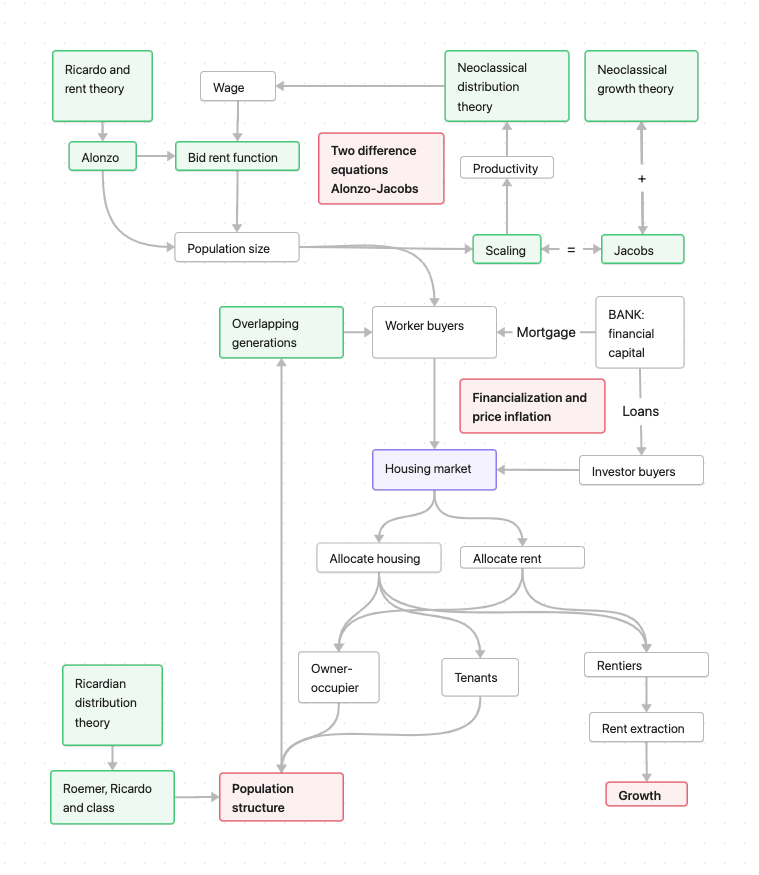
\includegraphics[scale=.6]{fig/flow-full-model.png}
\label{Stylized model flow.}
%\pagestyle{headings}
% \usetikzlibrary{positioning}
%\begin{tikzpicture}[remember picture,overlay,shift={(current page.north east)}] \node[anchor=north east,xshift=-1cm,yshift=-1cm]{\includegraphics[width=1cm]{example-image-a}};\end{tikzpicture}
\end{adjustwidth}
\caption{Model logic }\label{fig-flow-full-model}
\end{figure}
}

\begin{enumerate}
\item We incorporate the spatial structure of the city and its transportation system using a version of the \gls{bid-rent function} that drives all Alonso-style models. This equation is embedded in the decision of every agent because it determines the economic rent for each piece of property.

\item We incorporate the fundamental wealth production process of the city using an \gls{urban scaling} law that captures Jacobs-style agglomeration effects. This allows us to bypass the complexities of labour and goods market adjustments and instead to deal with the underlying long-term relationship between city population and production. We call the combination of this Jacob agglomeration effect with the Alonso model an \gls{Alonso-Jacobs model}. Our \gls{agent-based model}, in effect, mimics two difference equations, operating on two aggregate variables, and incorporating the major insight of a half-century of \gls{neoclassical growth theory}.

\item To link the Alonso-Jacobs model to the financial system, we develop an \gls{overlapping generations} model of the housing market with borrowers and lenders that tracks ownership and wealth. This turns out to be the most detailed and computationally-intensive part of the model. To model the effects financializing housing in our \gls{agent-based model} we are forced to carefully specify the microeconomics of individual decisions. % In Section~\ref{section-micro},
We therefore, we describe the microeconomic objective function that individuals and our bank agent employ in deciding to purchase a property. 
\end{enumerate}

Figure~\ref{fig-flow-full-model} shows the model logic.  The following three sections will discuss each of the three primary components, the spatial structure, the productivity mechanism, and the housing market in order.  To focus the model on the core questions of the relationship between urban productivity and rent, we keep the first two components,  the spatial structure and the growth mechanism,  as simple as possible, modeling the market for housing in more detail. 

% ANALYSIS???Finally, in  Section~\ref{section-system} we explain how financialization might affect the housing market as a system and some consequences for society in general. %At that point we can introduce our specific hypotheses and how we intend to test them.

\section{Spatial structure}

% In this section, we introduce the basic structure of the model, drawing on the circular city model.  
%  
% We build a spatially explicit agent model where agents work in one location and incur costs travelling to work. This work integrates a model of production and labour into a standard spatial model of the city. In this section, we introduce an analytic model of production and a labour market in a stylized circular city. 

% \subsection{Labour supply for production}
We begin with a model of a circular city.\footnote{In our computational model we use a grid structure with  a block metric, which is computationally more convenient and provides a slightly more natural representation of the property structure of actual cities.} %- INTRO CITY/APPROACH?
In the \gls{Alonso model} \cite{alonsoTheoryUrbanLand1960, alonsoLocationLandUse1964}, firms are located at the centre of a circular city, the central business district. Residents live distributed across space, can take jobs, and commute to work at the urban center. 
% In the simplest version, firms concentrate at the city centre. Workers are spread over space and pay transportation costs to commute.



Firms produce perfectly \gls{substitutable} % For simplicity, firms produce a variety of
goods that they sell into a commodity market. Demand for the \gls{product} is \gls{perfectly elastic}, so the price remains constant. 
Firms purchase the time of workers. %to capture the product of their effective labour
%and enjoy the product of \gls{effective labour} . They can produce more goods by hiring additional workers. 
With the neoclassical model of distribution,\footnote{Clark's neoclassical assumption is that workers receive the value of their marginal product \cite{clarkDistributionWealthTheory1899}.} 
% We assume that the neoclassical model of distribution holds in the long run and 
workers receive the value of their marginal product. 
Because of agglomeration effects, workers in the city are more productive than workers in the countryside. They therefore receive an \gls{urban wage premium}.

% TODO this shows the dynamics of a local economy, trade dynamics dominate local dynamics in many cases, that is explored with the addition of more cities and centres. 
%NEED TO INTRODUCE SUBSISTENCE WAGE BEFORE MENTIONING IT ABOVE %[MAYBE This follows xyz's approach, and makes it possible to explore resident's choice to work]. 

As in the Alonso model, described in Chapter~\ref{chapter-space}. The \gls{urban wage premium} and transportation costs together determine both the radius of the circular city and the size of the labour force, %?There is no fixed boundary and the size of the city is determined by the utility that can be achieved in competing regions of competing for labour.
% and as in the standard circular city model the constraint on growth is provided by transportation costs, which limit the size of the commuter-shed and therefore the labour force at any wage. 
 %The raidus of the commuter shed is thus,  %The farthest workers will travel to work is thus 
% The  productivity of the city attracts people. 
since agents work if the wage premium is greater than the cost of travel. % Living close to work has value to workers because it saves the cost of transportation. 
The higher the wage, the farther workers will commute. %This is the core of the Alozo circular city model.
The farthest that workers will travel is $\frac{w}{{c}}$, where ${c}$ is the cost of transportation per unit distance. This defines the radius of the city and the commuter shed.

The \gls{urban labour supply} is an \gls{aggregate} measure that emerges from individual agents' choice to commute. Considering a standard, Alonzo-style \gls{circular city} with a uniform lot size, $s$, and  one worker per unit land. For illustrative purposes, the labour available is simply the area of the circle divided by the lot size 
\begin{equation}
%=  \frac{\pi}{s}(c^{max})^2	
 N = \frac{\pi}{s} \left(\frac{w}{{c}}\right)^2,
%   =\frac{\pi}{{c}^2 s} w^2,
\label{eqn-labour-supply1}
\end{equation}
where $\omega$ is the wage premium, $c$ is the cost of transportation, and $s$ is lot size (land per person).\footnote{The formula is for the case with a uniform density of one worker per lot. In the computation model density is a variable.} This is the equilibrium \gls{urban labour supply} function for the circular city. For a city with an idealized rectangular grid of streets, the city shape is rectangular rather than circular and the labour supply function is \[N= \frac{2}{s}\left(\frac{w}{{c}}\right)^2.\] %which is a \cite{GET_migration_equilibOR_pop_equilib_condition}. %It defines the quantity of labour available.

%\footnote{See the discussion of model extensions in Appendix~\ref{appendix-future-work}.}.
% To get the \gls{urban wage premium}, we can write the inverse of the labour supply function:
% \begin{equation}
% w= (\frac{ {c}^2s}{\pi})^{0.5} L^{0.5}.
% \label{eqn-inverse-labour-supply}
% \end{equation}

\section{Agglomeration and productivity}\label{sec:Production-fn}


% *** ADD BACK? To study the productivity of cities, we incorporate Jacobs-style agglomeration economies (\cite{beaudryWhoRightMarshall2009, vanderpanneAgglomerationExternalitiesMarshall2004, jacobsEconomyCities1969}), using an approach similar to the way the \gls{Solow-Swan model} incorporates labour-augmenting technical change with a \gls{Cobb-Douglas} production function, and building the production function into a standard Alonso-style model of an urban economy.
%, using a simple Cobb-Douglas production function. 
% We incorporate the estimated scaling relationship in 
%The scaling result at the level of the city allows us to incorporate the agglomeration effect in a \gls{circular city} model, 
The agglomeration effect that augments the productivity of workers means firms produce more goods with a given stock of labour if the city is larger and urban workers are more productive. Figure~\ref{fig-agglomeration-surplus} in Chapter~\ref{chapter-growth} illustrates the increasing returns to urban size. % than rural workers due to the positive agglomeration externalities. 
These increasing returns mean that urban firms can %Urban firms can therefore 
pay a premium that depends on, among other things,  the size of the city. Because workers face transportation costs, firms have to pay this premium to attract workers. % , above the subsistence wage.
%in a city with more people, as introduced in Chapter~\ref{chapter-growth} on growth.(**E SEE NOTE HERE) % #E i THINK YOU NEED TO FLESH THIS OUT, i'M NOT SURE EXACTLY WHAT YOU ARE SAYING. JUST BE A BIT MORE SPECIFIC AND FLESH OUT. 
% \subsection{Labour force}
%There are also firms that produce goods to sell. (???) % #E HOW IS THIS DIFFERENT THAN THE FIRMS PRODUCING GOODS IN THE PREVIOUS PARAGRAPH???

% Firms sell the goods they produce into a commodity market. 
 %, which are both exported and locally consumed 
% to sell into a large market, at a fixed price. 





To focus the model on urban productivity and the growing urban wage premium, we model workers as receiving a \gls{subsistence wage} $\psi$ in the countryside.\footnote{Classical economists employed the \gls{subsistence wage} assumption to simplify their analysis in a similar way.} % 
%\cite{GET_classical-subsistence-wage}.
%
% CLASSICAL POLITICAL ECONOMY, THE SUBSISTENCE ...
% American Economic Association
% https://www.aeaweb.org › conference › retrieve
% PDF he Classical Understanding of the Subsistence Wage. While the historical run of classical political economy runs from William Petty through David.
This subsistence wage could come from work in the local community, living off the land, family support, social support, or something else. 
 % The model is set up so that all of an urban  tenant's  income is spent on  basic living costs, $\omega$, transportation $td$ or rent. Disposable income for owner occupier $i$ is therefore just the return  $\omega -dc$ which may accumulate as a financial asset.
% To attract workers to live in the city and commute to the central business district, firms pay the  \gls{urban wage premium}, $\omega$, in addition to  the subsistence wage $\psi$. 
%\footnote{See parameter appendix Section~\ref{section-wage-premium} for a discussion of the empirical literature on the \gls{urban wage premium}.}. 
% When workers take a job, they give up the subsistence income and, % instead receive a wage from their employer. % When workers take a job, they  receive, in addition to the subsistence wage,  the wage premium  from their employer. 
Urban workers give up the subsistence income and receive the \gls{urban wage}, $\psi +  \omega$, the subsistence wage plus the \gls{urban wage premium} that firms pay to attract workers. 
% When we assume an subsistence wage with a specific share  applied to housing we are implicitly assuming that landlords are seeking to claim the value of the rents. It makes it possible to explore whether and how tenants and even owners may be squeezed towards a \gls{subsistence frontier}. %whatever value the can. % tenants are squeezed by landlords. % DOES THE 'THIS' REFER TO THE FORMALIZATION OF WARRANTED RENTS?

\subsection{Wage determination}

According to \gls{neoclassical distribution theory}, the firm maximizes profit by setting the marginal value of the product of each \gls{factor of production} equal to the unit cost per factor.\footnote{Appendix~\ref{appendix-firm-theory} has more detail on the theory of the firm underlying the treatment here.} If we calculate the physical marginal product of labour for the Cobb-Douglas with the Jacobs externality $A(L^T)$ from Equation~\ref{eqn-production-jacobs}, we get 
\begin{align}\label{eqn-model-MPL}
y              =&  A(L^T) k^\alpha n^\beta \nonumber\\ 
\die{y}{L}     =&\beta A(L^T) k(t)^\alpha n^{\beta-1} \nonumber\\
                =&\frac{\beta A(L^T) k(t)^\alpha n^\beta}{n} \nonumber\\
                =& \frac{\beta y}{n}.
\end{align}
This is clearly positive and increasing in $L^T$, the aggregate labour force for the city.  It follows that population growth increases marginal product in this model. 


Since optimizing firms are assumed to adjust their wage offer and hiring to achieve a wage that is equal to the  marginal \textbf{value} product of labour 
\begin{align}\label{eqn-model-MPL-w}
             \omega + \psi   =& P_y\frac{\beta y}{n}.
\end{align}
where $P_y$ is the price of output. We assume the price of output is constant and will treat it as \$1 per unit output for the rest of the chapter. As a result, the wage increases, perhaps with a lag, when urban population  rises 
\begin{equation}
 \die{(\omega + \psi)}{L^T} >0.
\label{eqn-wage-population}
\end{equation}
In our model the subsistence wage $\psi$ is fixed, so the wage premium must rise if the marginal product of labour rises.  We have shown that a rising wage premium increases the distance that workers will travel to work, so the city grows and population rises, as the upper loop in Figure~\ref{fig-flow-full-model} illustrates. 

 

Equation~\ref{eqn-model-MPL-w} is an equilibrium condition. Firms, however,  are agents setting wages and hiring while labour supply and demand are shifting.    We assume that they do know the marginal product of their current workforce and can observe the wage level from period to period. It is reasonable to assume that when their marginal product of labour rises they adjust both their labour demand and their wage offers. The marginal product of labour can be seen as a target wage. Equation~\ref{eqn-model-MPL-w} implies that the firm's target labour demand is 
\begin{equation}
           n  = \frac{\beta y}{\omega + \psi}.
\label{eqn-labour-demand}
\end{equation}
We assume it is reasonable to assume $\omega$, and the wage, $n$, the size of the firm's workforce,\footnote{The analytic model offers an equilibrium solution with full employment. The assumption of full-employment is uneralstic. Workers are laid off, and take time to find new employment. The time people spend moving between jobs causes frictional unemployment which varies with economic conditions. Introducing a constant or ``natural'' rate of unemployment %however, would have little effect on the overall behaviour of the model. Variable frictional unemployment 
would introduce additional dynamics, however it would be unlikely to affect the results that interest us.} 
both adjust slowly toward target values in each period. We also allow the number of firms to adjust gradually.\footnote{We have assumed that the firm does not notice that, by hiring, it increases the agglomeration effect for the city. This assumption is convenient as well as plausible since it removes a term, $\frac{\gamma Y}{N}$, that is quantitatively insignificant from the expression for the marginal product that guides firm behavior. If all firms are identical, the term becomes $F\frac{\gamma Y}{N} =\frac{\gamma Y}{L}$.}


% The city has single firm facing a fixed price for output. 

% IS THIS DUPLICATION? I THINK THE Solow-Swan model IS INTRODUCED IN SPACE CHAPTER. MOVE THIS TO SPACE CHAPTER IF NEEDED?
% In the \gls{Solow-Swan model}:
% \begin{equation} 
% Y(t) = K(t)^{\alpha}(A(t)L(t))^{\beta}
% \label{eqn-solow-swann}
% \end{equation}
% where $Y$, $K$ and $L$ are aggregate output, capital, and labour, respectively,  $A$ is the term the Solow-Swan model introduced for technology. The technology term capture the growth of labour productivity over time, $\alpha$ is the \gls{elasticity} of output with respect to capital, $\beta$ the elasticity of \gls{output} with respect to \gls{effective labour}, and $t$ time. If $\beta=1-\alpha$, this is a \gls{constant returns to scale} \gls{CRS} production function at the firm level.
% In the Solow-Swan model all factors of production are fully employed, and initial values $A(0)$, $K(0)$, and $n( 0 )$ are given. The number of workers, i.e. labour, as well as the level of technology grows exogenously at rate %s are $n$ and it   $g$,% respectively:  $L(t)=L(0)e^{nt}$     $A(t)=A(0)e^{gn}$ 
% This model uses a similar functional form to look at the effect of population density increasing % productivity. %how density increases in in  % It models how population increases productivity. 


%%%%%.   MAYBE REINTRODUCE THIS
% The urban wage premium scales with the agglomeration effect. The \glspl{agglomeration effect} ensure urban \gls{output} is more than proportional to urban population: 
%  \begin{equation}
%  Y\propto N^{\beta},
%  \label{eqn-production-population}
%  \end{equation}
% where $\beta$ is the elasticity of output with respect to capital, $\beta > 1$ where the agglomeration effect is positive. % Setting $\beta = 1$ would be the \gls{constant returns to scale}. $\beta - 1$ is the extra return that comes from adding to people the city. That return is the agglomeration effect that belongs to the city, it could go to the people.

% We can put this together using a model of the production function. We implicitly use a three-factor model of \gls{production}, where production, is a function of capital and labour as well as a third factor, a Solow-Swan style term for labour augmenting technical change, with an \gls{agglomeration} effect, $A(N)$, in place of technology, $A(t)$. Output is:

%\subsection{aggregate urban output}
% \begin{equation}
% Y=A()K^{\alpha }(L^\beta}.
% \label{eqn-prod1}
% \end{equation}
% where $K$ is capital, $\alpha$ is the elasticity of output with respect to capital, $\alpha = \beta - 1$, and  $n$ is the \gls{urban labour supply}. $A(N)$ incorporates Jacob-style agglomeration externalities. $A(N)N$ is \gls{effective labour}.\footnote{The function  was discussed in Chapter~\ref{chapter-growth}.}

% \section{Agglomeration Appendix: Production Function}
% SORT APPENDIX/OTHER STUFF

% The agglomeration factor increases with population. It multiplies labour because agglomeration scales the productivity of workers.  
% It is a model of a productive urban economy since the centre is productive and demands labour.
% The growth of population feeds back into productivity. % We allow rising population to directly increase the wage.  
% We supplement the spatial model with agglomeration effects consistent with the literature. % in the base model. 
% There is an agglomeration effect, which
% The agglomeration effect means firms can also produce more goods by operating in a city with more people, because of the connections and interactions between people (CITE). 
 
 %, we assume the presence of scaling, consistent with neoclassical growth models as discussed in Chapter~\ref{chapter-growth}. 
%In this section, we introduce the basic structure of the production side and connect it to the literature on urban scaling. 
% We bypass the complexity of modelling firms, allowing population increases to directly increase urban wage premium.
%, It is straightforward to compute the rate of excess return for  this model. 

% We assume that the firm behaves as a price taker in the labour market as well, despite the fact that we model it as a \gls{monopsonist}\footnote{}. JUSTIFY/REPHRASE/EXPLAIN monopsonist. %ALSO DOES THIS GO HERE OR BELONG WITH PRIOR SECTION?

% Labour demand is thus a derived demand based on standard neoclassical theory with an equilibrium wage offer that is the marginal (value) product of labour for the firm. Specifically, hiring proceeds until the marginal product of labour is equal to the wage.

% The firm adjusts its labour force upward when the \gls{marginal product of labour} is greater than the wage by selecting from its list of job applicants.
% The firm adjusts its wage offer upward when the marginal product of labour is greater than the wage and it faces a labour shortage.  Labour shortage is a situation where the firm wants to hire but its list of job applicants is empty.

 %The marginal product of labour at the firm level is increasing in $L^T$, at a decreasing rate to ensure a labour market equilibrium exists for the model %, to connect with the analytic tradition of economic modelling by ensuring there is an equilibrium level of production.  
 
% If the marginal product increased, then a firm that got large enough would out-compete smaller firms, hire all labour, always be able to produce more wealth by hiring more people, and would always produce more wealth by hiring people than by firing people. This doesn't happen. 
% Perhaps, the firm hires employees who best fit its needs first, but to grow, eventually it must hire less selectively. Finding markets may get harder with growth. Perhaps expansion adds additional costs, building a parking lot, administration, acquiring a larger building. Whatever the explanation, the marginal product of labour declines. 




% labour adjustment costs include moving costs for the employee or hiring, firing, or training cost for the firm. (there might be a hiring, firing, or training cost on the firm side, or on the employee side: expected time to employment costs, moving costs, etc.)
%The assumption of monotonically declining  marginal product of labour is embedded in the production function, so it applies in the analytic and agent models.  Agglomeration effects can push the sum above one. When the exponents add up to less than one, there are diminishing returns to scale.  Exploring alternatives would involved exploring other formulations of the production function.





\section{Housing market} \label{section-rent}
%Property markets are the largest and most complex part of our model. 
In this section, we describe the housing market sub-model model. %There is a great deal of detail simply because the market has different types of participants who consider a large number of variables and interact.
We have emphasized that urban properties generate economic surpluses that give rise to land rents. We therefore explicitly discuss land rents and their relationship to prices. In subsection~\ref{sec:warranted-rent} we begin by describing the stream of benefits that a property generates, including locational services, housing services and other amenities.  We describe the variables involved in calculating the value of a property based on these services. We term this the \gls{warranted rent}. Then in Subsection~\ref{sec:market-rent} we describe a simple model of the costs of providing housing to get a net value. 

{\color{red} I THINK IT WOULD BE HELPFUL TO REFER BACK TO THE COMMON USAGE OF RENT AND HOW THAT IS DINSTINCT YET SOMETIMES THE SAME AS ECON RENT. }

Because participation in the housing market depends on financing, in subsection~\ref{sec:mortgage-availability} we look in detail at the on mortgage availability. We distinguish economic benefits arising from the services provided by a property from the financial gains that ownership might provide, so in subsection~\ref{sec:bid-price} we model value  from the point view of an investor or non-resident owner and develop what we call a maximum bid price.  The maximum bid price provides one of the values for the bargaining model that we use to determine market prices. 

In subsection~\ref{sec:bargaining-model} we describe our price-determination mechanism, which is based on standard bargaining theory.  The rest of the chapter, subsection~\ref{sec:bids-and-reservation} derives specific bid and reservation prices for different agents.

 The explicit treatment of rents, prices, and  productivity \gls{premium} and use of the \gls{subsistence wage} as an analytical device  make this a `\gls{classical}' model despite its reliance on supply and demand modelling of the housing market.  To develop the analysis, we track the price and rent quantities, outlined in Table~\ref{table-price-notation}.\footnote{In the table, we include indices for agent $i$ and property $j$, for clarity. In the following development we'll only use the subscripts where needed to distinguish between agents and properties.}

% Rents go to the owners of a given property. If workers own their own homes, rents go to them. If others own the land, they can extract the rent. 
%In each period a house offers two kinds of services: {locational services} or  access to the central city job and amenities, and {home services}.  The {warranted rent} is the value of a complex stream of services. 


% *** TABLE ALSO NEEDS NET RENT $\mathcal{R}_N$ - WE SHOULD THINK ABOUT BEST WAY TO COMMUNICATE RELATIONSHIPS BETWEEN RENT TERMS.
\begin{table}[!ht]
\centering
{\renewcommand{\arraystretch}{1.6}
\begin{tabular}{r|c|c|c|c|c|c|c|}\cline{2-8}
       & Warranted  & Market & Expected & $i$'s Expected & Reservation & Asking & Bid     \\ \cline{2-8}
Price  & $P_{W_j}$      & $P_{M_j}$  & $P_{M_j}^\epsilon$ & $P_{M_{ij}}^{\epsilon}$     & $P_{R_{ij}}$       & $P_{A{ij}}$  & $P_{B{ij}}$   \\ \cline{2-8}
Rent  & $\mathcal{R}_{W_j}$      & $\mathcal{R}_{M_j}$  & $\mathcal{R}_{M_j}^\epsilon$ & $\mathcal{R}_{M_{ij}}^{\epsilon}$     &       &   &   \\ \cline{2-8}
% Rent $\mathcal{R}_W$ & $\mathcal{R}_W$ &        &       &             & $\mathcal{R}_M$ &          &               \\ \cline{2-8}
\end{tabular}
 }   

\caption{Price and rent notation}
% \caption{Price and rent notation\protect\footnotemark} % https://tex.stackexchange.com/questions/10181/using-footnote-in-a-figures-caption
\label{table-price-notation}
\end{table}
% There are three pieces to this analysis: there's the warranted price based on the underlying economic value of living in a property, the link here with urban productivity, there's the biding and negotiation process, and then there's the realized market price. 




\subsection{Warranted rent}\label{sec:warranted-rent}
\Gls{warranted rent} is the maximum rent that could be extracted from tenants for the stream of services provided by location and the housing supplied. In this case, the price to rent in the common usage is the same as the economic rent. A higher level of rent extraction would convince tenants they are better off leaving the city.\footnote{Abstracting from the adjustment process, the warranted rent can be thought of as a kind of \gls{attractor} or \gls{equilibrium} towards which prices evolve,  % independent of the tendencies of the market.  
Combining a model of long-run attractor dynamics with distributed agent interactions, combines the advantages of agent-based modeling and standard \gls{classical} and \gls{neoclassical} economic analysis to give insight into the dynamics of financialization. Appendix~\ref{appendix-methodology} on methodology discusses the approach.} 

Capozza et al \cite{capozzaFundamentalsLandPrices1989} show that land price has four additive components: the value of agricultural land rent, the cost of conversion, the value of accessibility, and the value of expected future rent increases. We treat the first two as constants. The value of accessibility  can be expanded to include amenities. In our base model the value is determined by the urban wage premium, which rests on the productivity of the city firms. %We include three distinct streams of services, the value of access to employment, which we call economic rent, locational amenities, and housing services.
Expected future price increases are driven by increases in the value of accessibility, which is to say, the rising productivity of the city. Productivity rises in our model due to pure agglomeration effects. Our concern is with what happens to the city and its people when financial capital captures the growing value generated by the agglomeration process.  


\subsubsection{Locational economic rent} \label{section-economic-rent}
The \gls{economic rent} is the value of surplus that arise from access to jobs in the centre of the city where agglomeration economies generate a wage premium. These are represented as %, on an annual basis, 
the wage premium, $\omega$, minus the transportation costs, $c$, for a property a given distance, $d$, from the center

\[\omega - {dc}.\]

\subsubsection{Locational amenity} \label{section-locational-rent}
The warranted locational rent includes  the economic rent as well as a locational amenity, $\mathbb{A}$. Locational amenity includes very local site-specific amenities like access to schools or views, as well as a general urban amenity function that is the value of living in a particular location $\mathbb{A}$. %For most of the discussion in this chapter we ignore locational amenities, although we make provision for them in our computational model.

\subsubsection{Housing services} \label{section-housing-services}
Housing services $\mathcal{H}_j$ are  tied to a particular property. They include the value of features like a building having a certain number of rooms, particular finishes, or landscaping, extensions or upgrades. To maintain our focus on locational rents, we simplify, fixing %the value of housing services, setting 
the value of the stream of housing services to a fraction $a$ of the subsistence wage, $a\psi$.

\subsubsection{Combined equation}
Combining the three streams, the economically \gls{warranted rent}, $\mathcal{R}_W$, is then %\footnote{The price a property might sell at would be $\omega - {dc} + \mathbb{A} + rural-op-cost + conversion cost$. For simplicity, we drop the last two terms. Conversion cost would be amortized over a very long period and would be small in any case. We have hidden the rural-op-cost in $a\psi$.} 
\begin{align}
\mathcal{R}_W=\omega - {dc} + \mathbb{A} + a\psi.
\label{eqn-warranted-rent}
\end{align}


\subsection{Market rent} \label{sec:market-rent}
The \gls{market rent}, $\mathcal{R}_M$, is what tenants actually pay. The market differs from the economically warranted rent as investors make individual decisions about rents, setting rents based on market conditions and their own expectations. If, for example, the price of output for firm falls, the value of labour for firms also falls and the number of workers will be reduced. The city would shrink and locational rents would fall. % As an initial approximation, we simplify, using the warranted rent to approximate the market rent:
% \[\mathcal{R}_{M, 0}= \mathcal{R}_W.\] 

As our simulation proceeds, the market price of land and market rental price generated by the agent-based housing market mechanism diverges from the economically warranted  rents and prices  because growth introduces an opportunity for speculation on future values.

\subsubsection{Net warranted rent} \label{section-net-rent}
Owners receive, not the total warranted rent, but the \gls{net rent} after expenses, including maintenance, taxes, and the cost of financing. The following sections detail the computation of each expense, and their combination into the net rent calculation.

\subsubsection{Annual taxation}
Owners pay property taxes\footnote{Property taxation is an entire field in economics, but we simply make provision for later work by including a term for taxes collected. How the taxes are spent will affect amenity and transportation costs.} based on appraised price, $P_{\tau}$
\begin{align*}
\mathcal{T} &= \tau  \mathcal{P}_{\tau}.
\end{align*}
where $\tau$ is the municipal tax rate or \gls{mill rate}, and the \gls{appraised value} is based somewhat approximately, and with a lag, on the \gls{market price}, so $\mathcal{P}_{\tau}$ is some fraction of $\mathcal{P}_{M, t-n}$.



\subsubsection{Annual maintenance}
Annual maintenance costs apply to buildings and lands but not to locational value, so it can be modeled as a share, $b$, of the housing services costs, $a \psi$ 
\begin{align}
\mathcal{O} &= a b \psi.
\end{align}

\subsubsection{Combined equation}
Combining, the \gls{net rent}\footnote{We are short-cutting the rent price formation process with a long-run equilibrium approximation based on the rents that can be extracted before people leave the city, so the mechanisms that push rent up to that extraction value are abstracted. Net warranted rent, $\mathcal{R}_N$, can diverge from market rent, $\mathcal{R}_M$, particularly in the short run, for many reasons. For instance, agents who have purchased a house may be able to pass a share of financing costs through to tenants as part of the market rent depending on their market power. Some workers may accept lower utilities or may have access to higher wages. %The market rent could include an additional term, $F(v, rM)$, where $F$ is a function of 
% Financing costs may be passed to renters, $F(v, rM)$, and depend on vacancy, $v$, interest rates, $r$, and the size of the mortgage, $M$.%how tight the market is, 
 %When all financing costs are passed on the tenant effectively buys the property for the investor. % The market rent is what an investor would use for price setting, 
% and we work with the net warranted rent in the price formation model. % There would be strong feedback from speculators taking on financing costs  to the level of rents for tenants, and this then feedback into prices. % These are distinct logics for the rent formation mechanism which can be explored through more explicit models of rental markets. Abstracting them gives a set of easily generalizable simplifications.% The way housing financing costs are passed through to tenants. are computed are detailed in the next sections.
% 
% Annual financing costs are $rM$. 
}is:

\begin{align}
\mathcal{R}_N &= \mathcal{R}_W - \mathcal{O} - \mathcal{T}.
\end{align}

 {\color{black}

\subsection{Mortgage availability} \label{sec:mortgage-availability}
% According to the Canada Housing Statistics Program (CHSP), first-time home buyers require a combination of sufficient income and savings in order to enter the housing market \cite{GET_REF}. In practice, 
Mortgage lenders often put two limits on the size of the mortgage, one based on wealth, a \textbf{wealth constraint}, and one based on income, a \textbf{carrying constraint} \cite{GET_REF_CHSP}. We have implemented these constraints by making both mortgage size and the interest rate on borrowing depend on income and wealth. As a result high-income and  wealthy agents can borrow larger amounts, at lower interest rates than the less wealthy.\footnote{The income constraint is sometimes called a housing expenditure share cap, and may be imposed to stabilize the hosing market. Gong and Leung \cite{yifangongDoesSpaceMatter2003} have investigated the distributional effects of income constraints.} %this lending policy.}


\subsubsection{Wealth-based mortgage maximum} 
% The availability of capital differs for rich and poor. 
We define household wealth, for the purpose of credit assessment, as

\begin{equation} 
W_i= P^{expected}_i - M_i  +S_i, 
\end{equation}
where $P^{expected}_i$ is the expected value of an existing owned home, $M_i$ is the mortgage on the home, and $S_i$ is personal savings, including the net value of assets other than the home. % = $age*savings\ rate* income$. ($M_i$ is relevant and requires calculation for cases where an existing  mortgage has not been fully paid off. and  someone wants a second mortgage for a revenue property.
For a newcomer who owns a rural home and owes no mortgage, the value of the rural home is simply the capitalized value of rural housing services
\begin{equation} 
P^{expected}_i = \frac{a\psi}{r}.
\end{equation}


    \begin{figure}[htb]
    \begin{center}
    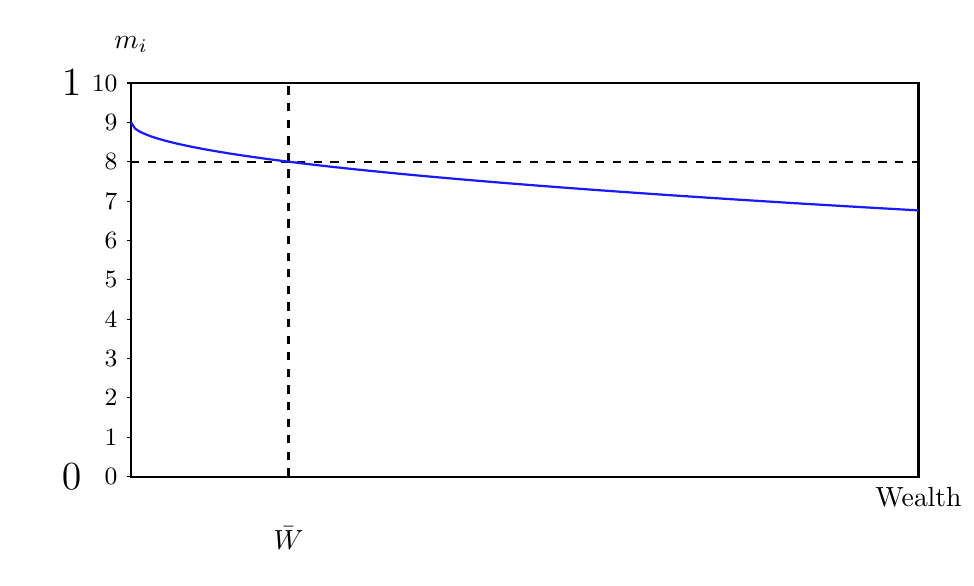
\begin{tikzpicture}[scale=.5]
% \def\bndmax{5}        %https://tex.stackexchange.com/questions/68462/filling-a-complex-region-with-tikz
% \def\bndmin{0.2}
\def\Y{10}  % height of y axis pecent
\def\W{20}  % length  of x axis
\def\Wbar{4}
\def\rbar{8}% this is the prime rate
% Equation   \[ r_i = (A + .5 \frac{\bar{W}}{W_i})\omega\]
% \def\Wmin{.63}  %This sets the lower limit fo the 
\def\Wmin{(\B*\Wbar)/(\Y/\rbar-\A)} %function to keep in in bounds
\tikzset{func/.style={thick,color=blue!90}}	
\draw [thick](\W,\Y)-- (0,\Y)node[left=.5cm]{\Large$1$}node[above=.25cm]{$m_i$} -- (0,0)node[left=.5cm]{\Large$0$}--(\W,0)node[below]{Wealth}--cycle;  	% Axes box
\draw [dashed, thick] (0,\rbar) -- (\W,\rbar);  	% Axes
\draw [thick,dashed] ( \Wbar,0)node[below=.5cm]{$\bar{W}$} -- (\Wbar,\Y);  	% Axes
\foreach \yi in {0,...,\Y} \draw (0,\yi)--(-.1,\yi)node[left]{\small$\yi$};
% \foreach \yi in {0,2,4,6,8,10} \draw (0,\yi)--(-.1,\yi));
% node[left]{\small$\yi$};
% \foreach \yi in {0,2,4,6,8,10}node at (-.1,yi) {{10*yi}} ;
\draw[func,domain=0:\W] plot [samples=200] (\x,(9-\x^.5/2);
\end{tikzpicture}
    \end{center}
    \caption{Individual borrowing ratio $m_i$ as a function of wealth}
    \label{fig-borrowing-ratio}
    \end{figure}


The borrowing ratio, $m$ is the fraction of a property's price that can be mortgaged. We assume that the bank uses a function of the form 


\begin{align}
m_i^{max\_permitted} =& \mathrm{max\_mortgage\_share} - 0.1*\left(\frac{\bar W}{ W_i}\right), \label{eqn-wealth-based-mortgage}  %^{\mathrm{wealth\_sensitivity}
\end{align} 
where $\bar{W}$ is mean wealth and $W_i$ is individual wealth.\footnote{To shift the curve  so that the curve approaches $m=0$ when $W=0$ we add  $Z=(1-m^{max})\bar W$ to the numerator and the denominator. The value is calculated by solving Equation~\ref{eqn-wealth-based-mortgage} for {$m_i^{max}=0$}.}


\subsubsection{Income-based mortgage maximum}
A common rule is that mortgage payments cannot exceed some fraction of income, $Y_i=\omega+ \psi + {r}S_i$, where $S_i$ is individual savings.
If $\mathbb{C}$ a person's carrying capacity, this gives us an \textbf{income-based  mortgage maximum} of 


\begin{equation}
M^{max}_{Y,i} = \frac{\mathbb{C} (\omega+ \psi + {r}S_i)}{r^{prime}},\label{eqn-income-based-mortgage}    
\end{equation}
% In addition, The Bank may have a maximum share of the price that it will lend, say $0.8P$. Because the actual price is unknown when buyers prequalify, this test limits the maximum bid computed below: \
% \[M^{max}i = min\left\{\frac{0.28*(\omega+w)}{r},  0.8P_0 \right\} \]
where ${r}$ is $i$'s rate of return on savings $S$ as the maximum a  buyer should pay. %\footnote{We  assume that the bank does not take transportation costs into account  when calculating income.}
%\footnote{If the expected return on a property is greater than the individual cost of borrowing, it would pay any agent to borrow as much as possible and purchase properties as they can available.}
In our model the bank uses a rule of this form to decide how much it is willing to lend to $i$.

  \begin{figure}
    \centering
    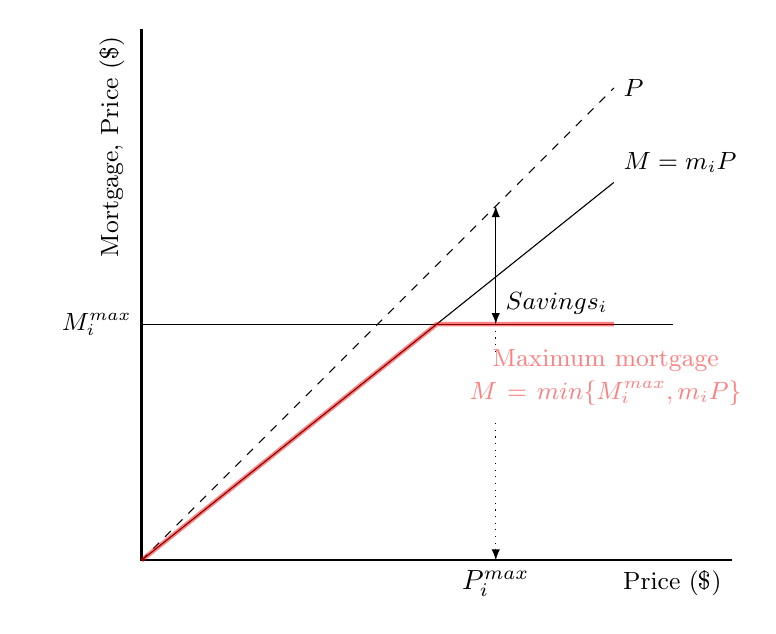
\begin{tikzpicture}	[scale=1.5]
%AXES
\draw[thick] (0,4.5) --(0,0)--(5,0)node[below left]{\small Price (\$)};
\node at (-.25, 3.5)[ rotate=90]{\small Mortgage, Price (\$)};
% M =Mi MAX
\draw[dashed] (0,0)--(4,4)node[right]{\small $P$};
\draw[] (0,2)node[left]{\small $M_i^{max}$}--(4.5,2);%node[right, red]{\small $M = M_i^{max}$};
% M =mi MAX
\draw[] (0,0)--(4,3.2)node[above right]{\small $M = m_iP$};
% COMBINED MAX RED
\draw[ultra thick, red, opacity=.5] (0,0)--(2.5,2)node[below right,  text width=4cm, align = center]{\small \\ Maximum mortgage \\ $M=min\{M_i^{max}, m_iP\}$}--(4.0,2);
% SAVINGS
\draw[latex-latex] (3,2)node[above right] {\small $Savings_i$}--(3,3);
% PMAX
\draw[dotted,latex- ] (3,0)node[below] {$P_i^{max}$}--(3,1.2);
\draw[dotted ] (3,2)--(3,1.72);
\end{tikzpicture}
    \caption{The bank's dual mortgage constraint and the savings constraint determine the maximum bid price}
    \label{fig:dual-constraint}
    \end{figure}

\subsubsection{Combined mortgage maximum permitted by the bank for new buyers and second home buyers}

The above  two equations specify two constraints on the mortgage.  Combining, we get 
\begin{align} 
M_i^{max} &= min \left\{ m_i^{max}*P, \ M^{max}_{Y,i} \right\}. 
\label{eqn-max-mortgage-combined}
\end{align}
The two constraints on  mortgage size that the bank imposes are incorporated in the  red line in Figure~\ref{fig:dual-constraint}. The maximum  permitted mortgage is thus combined with the savings constraint to determine the maximum price that a potential home buyer can offer. The top dashed diagonal line, in Figure , is the price, $P =$ mortgage $+$ savings. The difference between the two diagonal lines is what the purchaser pays from savings. %\footnote{Equation~\ref{eqn-property-investment-return2} implies a `bang-bang' control---with all sales going to the richest participant unless there are limits on the size of capital flows. For our simulation, we implement such limits.} 
% \[M^{max}_{UY,i} = \frac{0.28*(\omega+ \psi)}{r}\] 
% It is the maximum the bank will let you pay.

% \subsection{The cost of capital}
% The cost of capital is known to differ for rich and poor. This model ties the individual cost of capital,  ${r}$ for agent $i$, to a prime rate, $\bar r$, and to individual wealth. Figure~\ref{fig-borrowing-cost} illustrates the cost of the borrowing model we implement, 
%  \[ {r} = (A + B \frac{\bar{W}}{W_i})\omega\]
% Where $\bar{W}$ is mean wealth and $W_i$ is individual wealth.   
% a kink because there are 2 constraints.  The actual mortgage must be below both lines.
% This is just the constraint. Up to the kink, little $m_i$ is a fraction of price. beyond at little $m_i$ becomes a different number - number based on little $m_i$ for everyone
% banks have an advantage since they can practically bid anything
% m - mortgage share
% P - realized price
% M - maximum - 
% \begin{figure}[!ht]
% \begin{center}
% 
% Large version
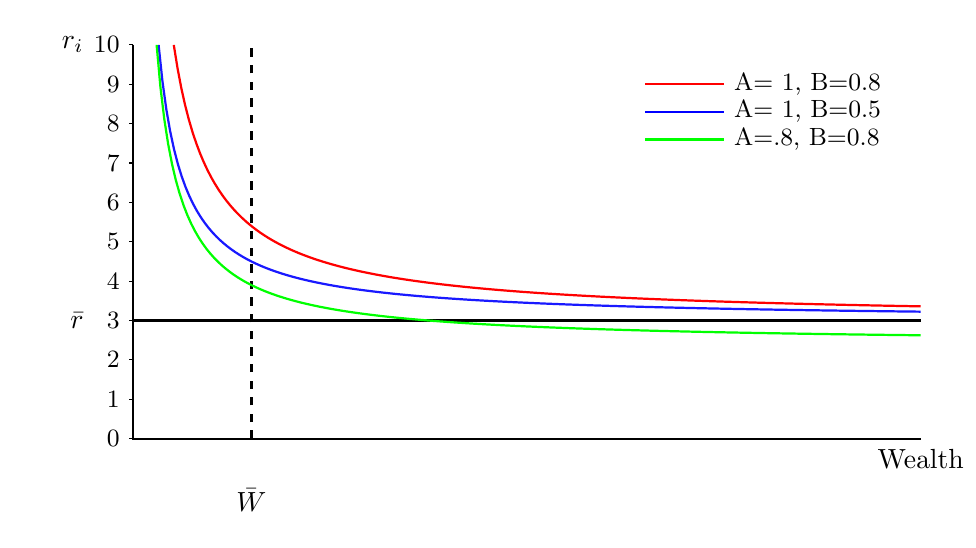
\begin{tikzpicture}[scale=.5]
%\def\bndmax{5}        %https://tex.stackexchange.com/questions/68462/filling-a-complex-region-with-tikz
%\def\bndmin{0.2}
\def \Y {10}  % height of y axis pecent
\def \W {20}  % length  of x axis
\def \Wbar {3} % jmeam wealth
\def \omega {3}
\def \A {1}  %was .5
\def \B {.5}
%Equation   \[ r_i = (A + .5 \frac{\bar{W}}{W_i})\omega\]
\def \Wmin{.63}  %This sets the lower limit fo the 
\def \Wmin{(\B*\Wbar)/(\Y/\omega-\A)} %function to keep in in bounds
	
\tikzset{func/.style={thick,color=blue!90}}	

\draw [thick] (0,\Y)node[left=.5cm]{$r_i$} -- (0,0)--(\W,0)node[below]{Wealth};  	% Axes
\draw [thick] (0,\omega)node[left=.5cm]{$\bar r$} -- (\W,\omega);  	% Axes
\draw [thick,dashed] ( \Wbar,0)node[below=.5cm]{$\bar{W}$} -- (\Wbar,\Y);  	% Axes

\foreach \yi in {0,...,\Y} \draw (0,\yi)--(-.1,\yi)node[left]{\small$\yi$};

\draw[func,domain=\Wmin:\W] plot [samples=200] (\x,{(\A+\B*\Wbar/\x)*\omega});
\def \A {.8}
\draw[func,domain=\Wmin:\W, green] plot [samples=200] (\x,{(\A+\B*\Wbar/\x)*\omega});

\def \A {1}
\def \B {.8}
\draw[func,domain=\Wmin:\W, red] plot [samples=200] (\x,{(\A+\B*\Wbar/\x)*\omega});

\draw [red,  thick](13, 9)--(15,9)node [right, black] {\small A=\ 1,\ B=0.8};
\draw [blue,  thick](13, 8.3)--(15,8.3)node [right, black] {\small A=\ 1,\ B=0.5};
\draw [green, thick](13, 7.6)--(15,7.6)node [right, black] {\small A=.8, B=0.8};
\end{tikzpicture}

% % Small version with equation and parameter values
% \[   r^h=\frac{ \delta(1+\dot p  - (1+r)m) \ + \rho   	-\kappa - t } {1-m}    \]
% \begin{tikzpicture}[scale=.35]
% %\def\bndmax{5}        %https://tex.stackexchange.com/questions/68462/filling-a-complex-region-with-tikz
% %\def\bndmin{0.2}
% \def \Y {10}  % height of y axis percent
% \def \W {18}  % length  of x axis
% \def \Wbar {3} % j mean wealth
% \def \omega {3}
% \def \A {1}  %was .5
% \def \B {.5}
% %Equation   \[ r_i = (A + .5 \frac{\bar{W}}{W_i})\omega\]
% \def \Wmin{.63}  %This sets the lower limit fo the 
% \def \Wmin{(\B*\Wbar)/(\Y/\omega-\A)} %function to keep in in bounds
	
% \tikzset{func/.style={thick,color=blue!90}}	

% \draw [thick] (0,\Y)node[left=.5cm]{$r_i$} -- (0,0)--(\W,0)node[below]{Wealth};  	% Axes
% \draw [thick] (0,\omega)node[left=.5cm]{$\bar r$} -- (\W,\omega);  	% Axes
% \draw [thick,dashed] ( \Wbar,0)node[below=.5cm]{$\bar{W}$} -- (\Wbar,\Y);  	% Axes

% \foreach \yi in {0,...,\Y} \draw (0,\yi)--(-.1,\yi)node[left]{\tiny$\yi$};

% \draw[func,domain=\Wmin:\W] plot [samples=200] (\x,{(\A+\B*\Wbar/\x)*\omega});
% \def \A {.8}
% \draw[func,domain=\Wmin:\W, green] plot [samples=200] (\x,{(\A+\B*\Wbar/\x)*\omega});

% \def \A {1}
% \def \B {.8}
% \draw[func,domain=\Wmin:\W, red] plot [samples=200] (\x,{(\A+\B*\Wbar/\x)*\omega});

% \draw [red,  thick](10, 9)--(12,9)node [right, black] {\tiny A=\ 1,\ B=0.8};
% \draw [blue,  thick](10, 8)--(12,8)node [right, black] {\tiny A=\ 1,\ B=0.5};
% \draw [green, thick](10, 7)--(12,7)node [right, black] {\tiny A=.8, B=0.8};

% \def \W {19}  % length  of x axis
% \node[right] at (\W,9.5){\small$\delta=$discount factor};
% \node[right] at (\W,8.5){\small$\dot p=$appreciation rate};
% \node[right] at (\W,7.5){\small$r=$borrowing rate};
% \node[right] at (\W,6.5){\small$m=$mortgage/price};
% \node[right] at (\W,5.5){\small$\rho=$rental  rate};
% \node[right] at (\W,4.5){\small$\kappa=$op cost rate};
% \node[right] at (\W,3.5){\small$t=$tax rate};
% \node[right] at (\W,2.5){\small$\upsilon=$use value rate};
%  \end{tikzpicture}



% One blue line with x-shift, y-shift
% \begin{figure}
% \begin{tikzpicture}[scale=.5]
% %\def\bndmax{5}        %https://tex.stackexchange.com/questions/68462/filling-a-complex-region-with-tikz
% %\def\bndmin{0.2}
% \def \Y {10}  % height of y axis pecent
% \def \W {20}  % length  of x axis
% \def \Wbar {3} % meam wealth
% \def \rbar {3}% this is the prime rate 

% %\def \Wmin{(\B*\Wbar)/(\Y/\rbar-\A)} %function to keep in in bounds
% \tikzset{func/.style={thick}}	
% 	% Axes
% \draw [thick] (0,\Y)node[left=.5cm]{$r_i$} -- (0,0)--(\W,0)node[below]{Wealth};  
% \foreach \yi in {0,...,\Y} \draw (0,\yi)--(-.1,\yi)node[left]{\small$\yi$};
% \draw [thick] (0,\rbar)node[left=.5cm]{$\bar r$} -- (\W,\rbar);  	% Axes
% \draw [thick,dashed] ( \Wbar,0)node[below=.5cm]{$\bar{W}$} -- (\Wbar,\Y);  	% 

% \def \A {1} %vertical shift aroung \rbar, the prime rate
%  \def \B {1}  % Scales the exponential curveBLUE
%  \def \C {1}  %right shift  
% % \def \Wmin {.4+\B}  %This sets the lower limit fo the 
% \def \Wmin {(\B*\Wbar)/(\Y-\rbar+\A) +\C} %function to keep in in bounds

% \draw[func,domain=\Wmin:\W, color=blue!90] plot [samples=200] (\x,{\rbar-\A+\B*\Wbar/(\x-\C))});
% \node  [align=left, text width =2cm ] at (13, 8.3) {\small y-shift=\A \newline scale=\B \newline x-shift= \C};

%  \end{tikzpicture}
% \caption{Individual borrowing cost as a function of wealth II}
% \label{fig-borrowingrate2}
% \end{figure}

% The rates $\delta,\ \sigma,$ and $r$ depend on the period, $T$. 


% LARGE WITH DIFFERENT PARAMETER VALUES THAN MAOIN FIGURE - MORE SPREAD

% \begin{figure}
% \begin{tikzpicture}[scale=.5]
% %\def\bndmax{5} % https://tex.stackexchange.com/questions/68462/filling-a-complex-region-with-tikz
% %\def\bndmin{0.2}
% \def \Y {10}    % height of y axis as a pecent
% \def \W {20}    % length  of x axis
% \def \Wbar {3}  % mean wealth
% \def \rbar {3}  % the prime rate 

% % Equation   \[ r_i = (A + .5 \frac{\bar{W}}{W_i})\omega\]
% \def \Wmin{.63}  %This sets the lower limit fo the 
% \def \Wmin{(\B*\Wbar)/(\Y/\rbar-\A)} %function to keep in in bounds
% \tikzset{func/.style={thick}}	

% % Axes
% \draw [thick] (0,\Y)node[left=.5cm]{$r_i$} -- (0,0)--(\W,0)node[below]{Wealth};  
% \foreach \yi in {0,...,\Y} \draw (0,\yi)--(-.1,\yi)node[left]{\small$\yi$};
% \draw [thick] (0,\rbar)node[left=.5cm]{$\bar r$} -- (\W,\rbar);  	% Axes
% \draw [thick,dashed] ( \Wbar,0)node[below=.5cm]{$\bar{W}$} -- (\Wbar,\Y);  	% 

% \def \A {1.0}  \def \B {0.5} %BLUE
% \draw[func,domain=\Wmin:\W, color=blue!90] plot [samples=200] (\x,{(\A+\B*\Wbar/\x)*\rbar});
% \draw [ultra thick, color=blue!70 ](13, 8.3)--(15,8.3)node [right, black] {\small A=\A,\ B=\B};

% \def \A {0.5} 
% \def \B {0.5} % GREEN
% \draw[func,domain=\Wmin:\W, color=green] plot [samples=200] (\x,{(\A+\B*\Wbar/\x)*\rbar});
% \draw [thick,  color=green](13, 7.6)--(15,7.6)node [right, black] {\small A=\A, B=\B};

% \def \A {1.0}  \def \B {0.8} % RED
% \draw[func,domain=\Wmin:\W, red] plot [samples=200] (\x,{(\A+\B*\Wbar/\x)*\rbar});
% \draw [thick,  color=red](13, 9)--(15,9)node [right, black] {\small A=\A,\ B=\B};
% % KEY
% \end{tikzpicture}
% \caption{Individual borrowing cost as a function of wealth}
% \label{fig-borrowingrate1}
% \end{figure}
% Figure of cost of borrowing
% \caption[Borrowing cost for agents depending on wealth.]{Borrowing cost for agents depending on wealth, with different values for parameters $A$ and $B$ in Equation~\ref{eqn-interest-wealth-relationship}.} %$A=1$  $B=0.5$ (blue);  $A=1$  $B=0.8$ (red), and  $A=.8$  $B=0.8$ (green).}
% \label{fig-capital-cost}
% \end{center}
% \end{figure}

\subsubsection{Individualized borrowing rates} \label{sec:borowing-rate}

    \begin{figure}
    \centering
    
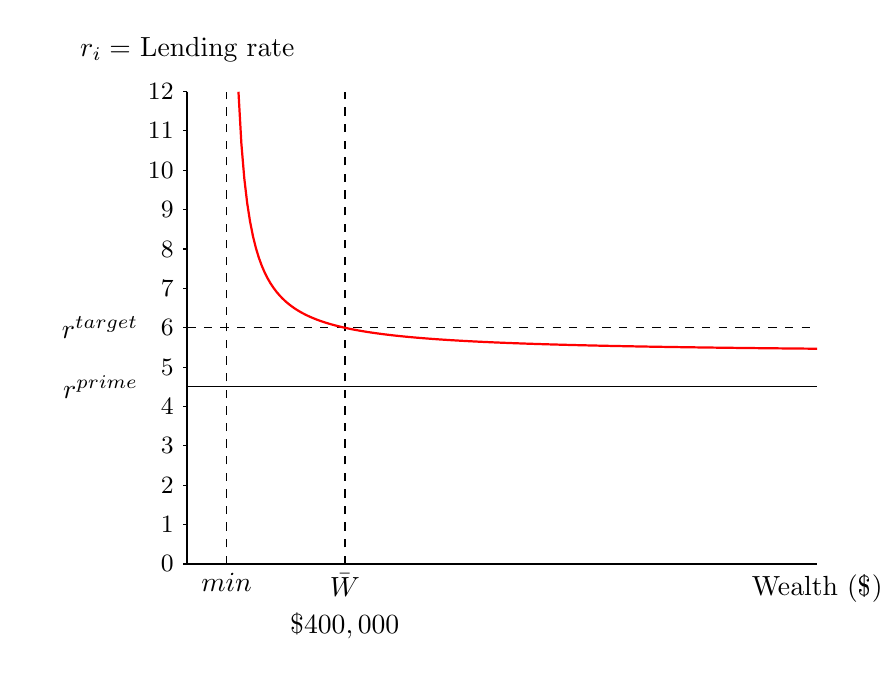
\begin{tikzpicture}[scale=.5].  %  Individual borrowing rate r\_i
%\def\bndmax{5}        %https://tex.stackexchange.com/questions/68462/filling-a-complex-region-with-tikz
%\def\bndmin{0.2}

\def \k {2}    % budget for rectangular hyperbola
\def \Wbar {4} % meam wealth in hundred thousands
\def \Wmin {1} % This sets the lower limit for lending in hundred thousands
\def \W {16}    % length  of x axis
\def \rbar {4.5} % N.B.:  this is r bar
\def \Y {12}     % height of y axis percent
\def \margin {1.5}
\def \target {\margin+\rbar} % target interest rate for bank
\def\bndmin {0.3} % This limits the function on the right so that it stays in the plotting frame
%\def \Wmin{(\B*\Wbar)/(\Y/\rbar-\A)} %function to keep in in bounds. NEEDS WORK
	
\tikzset{func/.style={thick}}	
\draw [thick] (0,\Y)node[above=.25cm]{$r_i=$ Lending rate} -- (0,0)--(\W,0)node[below]{Wealth (\$)}node[below=.5cm] {};   	% Axes

\draw [thin] (0,\rbar) node[left=.5cm]{$r^{prime}$} -- (\W, \rbar);  	% % bank rate line
\draw [thin, dashed] (0,\target) node[left=.5cm]{$r^{target}$} -- (\W, \target);  	% % target rate line
\node at ( \Wbar, 0)[below=.5cm]{$\$400,000$};  
\foreach \yi in {0,...,\Y} \draw (0,\yi)--(-.1,\yi)node[left]{\small$\yi$};  %$ put the scale on the y axis

\draw [thick, dashed] (\Wbar, 0)node[below] {$\bar{W}$} --  (\Wbar, \Y);  	%. Wbar
\draw [thin, dashed]  (\Wmin, 0)node[below] {$min$} -- (\Wmin, \Y);  %minimum lending wealth

\draw[func,domain={\W-\Wmin}:\bndmin, red] plot [samples=200] (\x+\Wmin,{\target+\k/\x - \k/(\Wbar-\Wmin)});

\end{tikzpicture}


% \begin{tikzpicture}[scale=.5]
% %\def\bndmax{5}        %https://tex.stackexchange.com/questions/68462/filling-a-complex-region-with-tikz
% %\def\bndmin{0.2}
% \def \Y {10}  % height of y axis pecent
% \def \W {20}  % length  of x axis
% \def \Wbar {4} % jmeam wealth
% \def \omega {3} % N.B.:  this is r bar

% %Equation   \[ r_i = (A + .5 \frac{\bar{W}}{W_i})\omega\]
% \def \Wmin{.63}  %This sets the lower limit fo the 
% \def \Wmin{(\B*\Wbar)/(\Y/\omega-\A)} %function to keep in in bounds
	
% \tikzset{func/.style={thick}}	

% \draw [thick] (0,\Y)node[left=.5cm]{$r_i$} -- (0,0)--(\W,0)node[below]{Wealth};  	% Axes
% \draw [thick] (0,\omega)node[left=.5cm]{$\bar r$} -- (\W,\omega);  	% Axes
% \draw [thick,dashed] ( \Wbar,0)node[below=.5cm]{$\bar{W}$} -- (\Wbar,\Y);  	% Axes

% \foreach \yi in {0,...,\Y} \draw (0,\yi)--(-.1,\yi)node[left]{\small$\yi$};

% %     ORANGE
% % \def \A {1} \def \B {.8}
% % \draw[func,domain=\Wmin:\W, orange] plot [samples=200] (\x,{(\A/\x+\B*\X/\Wbar/\x)*\omega});
% % \def \A {1} \def \B {.1}
% % \draw[func,domain=\Wmin:\W, orange, dashed] plot [samples=200] (\x,{(\A+\B*\X/\Wbar/\x)*\omega});

% %     RED
% \def \A {1} \def \B {.8}
% \draw[func,domain=\Wmin:\W, red] plot [samples=200] (\x,{(\A+\B*\Wbar/\x)*\omega});
% \def \A {1} \def \B {.1}
% \draw[func,domain=\Wmin:\W, red, dashed] plot [samples=200] (\x,{(\A+\B*\Wbar/\x)*\omega});

% %.    BLUE
% \def \A {1} \def \B {.5}
% \draw[func,domain=\Wmin:\W, blue!90] plot [samples=200] (\x,{(\A+\B*\Wbar/\x)*\omega});
% %     GREEN
% \def \A {.8} \def \B {.8}
% \draw[func,domain=\Wmin:\W, green] plot [samples=200] (\x,{(\A+\B*\Wbar/\x)*\omega});
% %.    BLACK
% \def \A {.5} \def \B {.5}
% \draw[func,domain=\Wmin:\W, black] plot [samples=200] (\x,{(\A+\B*\Wbar/\x)*\omega});


% \draw [red,  thick](13, 9)--(15,9)node [right, black] {\small A=\ 1,\ B=0.8};
% \draw [red,  thick, dashed](13, 9.7)--(15,9.7)node [right, black] {\small A=\ 1,\ B=0.1};
% \draw [blue,  thick](13, 8.3)--(15,8.3)node [right, black] {\small A=\ 1,\ B=0.5};
% \draw [green, thick](13, 7.6)--(15,7.6)node [right, black] {\small A=.8, B=0.8};
% \draw [black, thick](13, 6.9)--(15,6.9)node [right, black] {\small A=.5, B=0.5};
% \end{tikzpicture}


\label{fig-capital-cost}
    \caption{Individual borrowing rate $r_i$ price of capital}
    \label{fig:Wealth-based}
    \end{figure}

The cost of capital differs for rich and poor. We tie the individual cost of capital %,  ${r}$, for agent $i$ 
to the lender's target rate $r^{target}$, and to individual wealth. Figure~\ref{fig-capital-cost} illustrates the cost of the borrowing model we implement, which is  roughly consistent  with the stylized facts about lenders. 
 
\begin{equation}
{r} = r^{target}+ K/(W-W_{min}) -K/(\bar W - W_{min})\label{eqn-interest-wealth-relationship}
\end{equation}
for $W>W_{min}$, where  $r^{target}$ is the bank's target rate of return,  $\bar{W}$ is mean wealth and $W_i$ is individual wealth, $W_{min}$ is the level of wealth the bank requires to lend at all, and $K$ is a parameter for the wealth-sensitivity of lending. The denominator in the last two terms is simply wealth above the lender's minimum. We assume that the wealthy are lower risk borrowers and are given preference on rates. The final term ensures that the target rate is charged for borrowers with average wealth.


%The individual cost of capital,  ${r}$ for agent $i$ is tied to a prime rate, $\bar r$ or the bank's target rate, $r^{target}$, and and varies with individual wealth. %Figures~\ref{fig-borrowing-rate1} % and ref{fig-borrowing-rate1} 
%illustrates a  possible  cost-of-borrowing models 

% \begin{align}
%  {r} =  &  \left(A + B \frac{\bar{W}}{W_i}\right) \bar r       \label{eqn-incomeandr1}  \\
%  {r} =  &  \left(\bar r - A + B *\frac{\bar W}{W_i - C}\right) \label{eqn-incomeandr2}  \\
% \end{align}
% Where $\Bar{W}$ is mean wealth and $W_i$ is individual wealth. In Equation~\ref{eqn-incomeandr2},  A determines y-shift, B, the scale, and C the  x-shift for the curve.


\subsubsection{New: Declining principle}\label{sec:declining-principle}

Mortgages are renewed after $\mathbb{T}$ years. During that period some of the principle has been paid off. This is most important when a property is sold. The seller gets $P-M_{i,\mathbb{T}}$, where  $M_{i,\mathbb{T}}$ is its remaining mortgage.

% % {\color{red} 

% **** ADD BACK
% \textbf{Footnote on size of mortgage at renewal.}
% % \footnote{We would need to calculate the decline balance when  renewal came up to know what assets a person has. We need a function that gives us the size of the mortgage remaining at each renewal or at the time of sale, $M_{i,term}$, for each subsequent renewal. The  function depends on the mortgage renewal term, $\mathbb $, the number of terms $term$  that have passed since the purchase, the interest rate ${r}$ and the payment. Mortgages are usually intended to be paid off over, say,  $L=25$ years If we use $T=5$, there will be 4 renewals and the house will b =e paid off at the end of the fifth. Payments are larger than the interest, so the amount owed at the end of each month declines. At the end of month N it is

% % There is a standard formula for choosing the payment so that the mortgage it is paid off at the end of the mortgage life, $L$. Say $n$ is the number of monthly payments (for example 25*12=300) %https://en.wikipedia.org/wiki/Mortgage_calculator

% % \[payment= {r}^\mathbb{\mathbb{T}}M \left[\frac{(1+{r}^\mathbb{T}\mathbb{T})^n}{(1+{r}^\mathbb{T})^n-1} \right]\]
% % Where ${r}^\mathbb{T}$ is the interest rate compounded for $\mathbb{T}$ periods.
% % % \begin{align}
% % % M_{N*T}&=(1+r)^{N}M_0-p_{N}c\nonumber \\
% % % &{}=(1+r)^{N}P-{\frac {(1+r)^{N}-1}{(1+r)-1}}c \nonumber\\
% % % &{}=(1+r)^{N}P-{\frac {(1+r)^{N}-1}{r}}c
% % % \end{align}
% % % Amount owed at end of month N}
% % %}
% % }
% % }

% \textbf{We can assume is paid off the mortgage when we discuss retirement decisions. If as person works 40 years and buys a house by the 15th year they will have paid off their  mortgage and collect the entire price if they sell. }  

% When else will we need to consider this problem? If we let people buy a revenue property - then wealth includes $P-M$. Also if we let people die early, or allow them to change homes part way through a career- for family reasons.


\subsection{Bid price}\label{sec:bid-price}
A bidding process determines the realized market price, with bidders taking into account potential capital gains. In this section, we describe the formation of the maximum bid price that we use in the bidding model. The maximum \gls{bid price}, $P_{B,ij}^{max}$ %, where i and j refer to the individual and the property involved,\footnote{We suppress the $ij$ identifiers for the rest of this chapter. }  
is the value of a property to the owner or to a potential buyer. It will differ across individuals depending on their cost of capital, discount rates,  savings, and access to mortgage funding. The same equation used to calculate the bid price used to compute the \gls{reservation price}, the minimum price that an owner will sell a property for. 

The model distinguishes between two types of investment buyers, institutional buyers and homeowners buying an investment home. They use the same investment formula, but may have different values of the parameters determining their bid prices.

We first calculate the net present value of the purchase, then divide by the amount of capital employed, which we assume is simply the size of the down payment made at the beginning of the period. This gives us a rate of return.\footnote{An alternative approach would be to calculate an \gls{internal rate of return} (IRR), but the IRR is in general the solution to a polynomial and does not guarantee a single-valued result \cite{robinsonOptimalTerminationIRR1996}. Multiple real-valued  IRRs may arise;  complex-valued IRRs may arise;  the IRR is, in general, incompatible with the \gls{net present value} (NPV) in accept/reject decisions; the IRR ranking is, in general, different from the NPV ranking; the IRR criterion is not applicable with variable costs of capital. Ways to salvage the IRR as a usable criterion have been proposed that are consistent with our approach \cite{magniAverageInternalRate2010}.} The rate of return on the investment must exceed some required rate of return. This condition allows us to calculate the maximum bid that will satisfy that criterion.}
% We assume that agent may be  speculating on potential \glspl{capital gain} as well as on the \gls{use value} or net market rent they get from the property. We therefore treat the purchase as an investment decision and compute a rate of return, $v$, conditional on the price paid. This allows us to 
We then solve this for the maximum bid, $P_{max}^{bid}$ that achieves the desired rate of return. 


% The underlying value of a home is the capitalized value of the services it provides, which are perpetual.  Rents, however, depend on urban productivity and may change over time. Any expected increase in future rents capitalized into the market price of a home as a capital gain for the owner. Home prices should respond to expectations.

% As Horowitz \cite{horowitzBiddingModelsHousing1986} notes, a prospective buyer considering a vector of attributes of the property, including the seller's asking price and the property taxes, transaction costs, and financing costs at a specified price. The  potential buyer also is likely to have estimates of the maintenance costs and resale value of the house, although these may be highly subjective. All of these factors shape whether an investment is profitable. To make a comparison with alternative investments, it is necessary to compute a rate of return.

The agent who purchases makes a down payment, $D$ on a house for a price, $P_0$, and agrees to pay off a mortgage, $M$ with interest at the end of the mortgage period.  The purchaser  receives the increased price 
$P_T = (1 + \dot P)^\mathbb{T}P_0 =(1+\dot P_\mathbb{T})P_0 $, 
after a period $\mathbb{T}$, Where $\dot P$  is the expected annual rate of price increase and we define $\dot P^\mathbb{T}$
or $\dot P^{^\mathbb{T}}$ 
as the $\mathbb{T}$-period  price-growth rate. The agent also receives either the net market rental value of the property throughout the period, $\mathcal{R}_N$, or if the owner is also the resident, the locational rents. 
 
% With a price-growth rate of $\dot P$ per year, the growth over $T$ years is $(1+\dot P)^\mathbb{T}$, and  %and a 5 year mortgage period, 
% the expected price at the end of the period is:

% \[P_M^{Te}=P_0(1+\dot P)^\mathbb{T}\]

% If, for example price growth is 10\%, $\dot P= 0.1$, the {capital gain}, or growth, over a 5-year mortgage term is 0.61051 $\approx$ 60\% of the original price, $P_0$.

%The expected rate of price growth, $P_{M_j}^\epsilon$, is an estimate based on rents and past market behaviour. In our computational model we employ a regression model to generate an \gls{expected market price} based on past prices. The rate of price growth $\dot P$ we use in our model of investor behaviour is derived from the same regression model.




% TODO SOME REFERENCES - what are these? MOVE? \cite{anselinModernSpatialEconometrics2014, gelmanDataAnalysisUsing2006}.


 
\subsubsection{Rent and mortgage costs}
Both mortgage payments and net rent revenue can be calculated as sum  of regular payments, each of which accumulates interest to the end of the mortgage period. This is called a ``uniform series compound amount.'' For net rent at the end of the mortgage renewal term we write\footnote{FIX Regular periodic payments collecting interest for a n periods yields CLARIFY/CHECK EQUATION t  $\frac{(1+r)^n-1}{r}$ times the payment amount is called a ``uniform series compound amount'' \cite{GET_SOURCE}.%source https://www.e-education.psu.edu/eme460/node/659
} 
\begin{equation}
\mathcal{R}_{N, \mathbb{T}}= \frac{(1+r)\mathbb{^\mathbb{T}}-1}{r}\mathcal{R}_N.     
\end{equation}

We can do the same calculation, we did above for net rents, for the mortgage payments.
The regular mortgage payment for each period is $rM=rmP_0$.\footnote{We assume that the regular payment covers only the interest and that the full mortgage is due at the end of the period.} Using the same calculation, the value of the mortgage payments is % and the uniform series compound amount for the mortgage, taking the same fraction of the regular payment amount. % This is the total cost of all mortgages payed over the term - there is a payment in each payment in each periodl Calculate the payment all the way to the end for each of them. There is interest, - summ all those payments with their different cost of money. - the sumation of allthe payments. 
\begin{equation}
\mathcal{M}_{\mathbb{T}} = \frac{(1+r)^\mathbb{T}-1}{r}rmP_0. 
\end{equation}
Both these amounts are discounted by $\delta^\mathbb{T}$ to the present. % in our calculation.
 
\subsubsection{The value of an investment with price growth or interest}
 The value $V$ of a property investment over a period of $\mathbb{T}$ years is  the capital gain, $P_{^\mathbb{T}}-P_{0}$, minus financing costs, plus net rent. % revenues.
% \[\mathcal{R}_{N, \mathbb{T}}=  \delta^\mathbb{T}\frac{(1+r)^\mathbb{T}-1}{r}\mathcal{R}_N  \]
% To keep the notation simple, let 
% \[\delta_r^\mathbb{T}=\delta^\mathbb{T}\frac{(1+r)^\mathbb{T}-1}{r}\]
% The present value of the mortgage repayment plus the accumulated interest be 
% \[\bar M^\mathbb{T}_r = \delta^\mathbb{T}\frac{(1+r)^\mathbb{T}-1}{r}\]
 We can write $V$ in terms of the purchase price, and several individual parameters: interest  rate, share of the price that can be mortgaged and  discount rate %\footnote{The down payment could be deducted in advance, but if the discount rate is equal to the interest rate it drops out completely.}
 
 \begin{align}
V &= \delta^\mathbb{T}\left( P_\mathbb{T}-P_0-\mathcal{M}_{\mathbb{T}}- M+ \mathcal{R}_{N, \mathbb{T}} \right)      \nonumber\\
&= \delta^\mathbb{T}\left( P_\mathbb{T}-P_0- \left(\frac{(1+r)^\mathbb{T}-1}{r}rmP_0\right)- M+ \mathcal{R}_{N, \mathbb{T}} \right)      \nonumber\\
&= \delta^\mathbb{T} \left(
\dot P_\mathbb{T} P_0 -\left((1+r)^\mathbb{T}-1\right)mP_0-mP_0
 +  \mathcal{R}_{N, \mathbb{T}} \right) 
%\label{first_sub}\nonumber
\\
  &= \delta^\mathbb{T} \left((\dot P_\mathbb{T} - (1+r)^\mathbb{T}m) P_0 + \mathcal{R}_{N, \mathbb{T}}\right),\label{eqn_investment_value}
\end{align}
where $\dot P_\mathbb{T}=\frac{P_\mathbb{T}-P_0 }{P_0}$  is the expected  change in the market price over the term of the mortgage as a fraction of the original price.
$V$ is the net present value of buying and selling after one mortgage renewal period of $\mathbb{T}$ years. %All rates are scaled to the length of the period to avoid the need for compounding calculations. 
% The function has four individualized parameters, $\delta$, $\dot p$, $r$, $m$. %, as well as any factors that affect the rent or other terms.


\subsubsection{Rate of return on investment}
We divide $V$ by the size of the down payment, $D=P_0-mP0$, to get the  rate of return  

\begin{align}
r^{return} =
  &= \frac{V}{D}  \nonumber \\
  &= \delta^\mathbb{T} \left((\dot P_\mathbb{T} - (1+r)^\mathbb{T})m \frac{P_0}{D} + \frac{\mathcal{R}_{N, \mathbb{T}}}{D}\right) \nonumber \\
%  &= \delta^\mathbb{T} \left((\dot P_\mathbb{T} - (1+r)^\mathbb{T})m \frac{P_0}{P_0-mP_0} + \frac{\delta_r^\mathbb{T}\mathcal{R}_{N, \mathbb{T}}}{P_0-mP_0}\right)\\
   &= \delta^\mathbb{T} \left((\dot P_\mathbb{T} - (1+r)^\mathbb{T})m \frac{P_0}{P_0-mP_0} + \frac{\mathcal{R}_{N, \mathbb{T}}}{P_0-mP_0}\right) \nonumber \\
  &= \frac{\delta^\mathbb{T}}{1-m} \left((\dot P_\mathbb{T} - (1+r)^\mathbb{T})m  + \frac{\mathcal{R}_{N, \mathbb{T}}}{P_0}\right).\label{eqn-property-investment-return1} 
\end{align}
Notice that the return depends on the price paid, $P_0$. 

\subsubsection{Capital gains tax}
The \gls{capital gains tax} is %one of the most interesting policy parameters to consider. It is 
a tax on the increase in value of a property that results form an increase in the price. The capital gains tax is a tax on speculative return on housing as an investment. In our model captures some or all of the expected gain from rising locational rents. We can introduce it in Equation~\ref{eqn-property-investment-return1} by multiplying $\dot P_\mathbb{T}$ by 1 minus the capital gains tax rate, representing the share of the capital gains that a buyer is permitted to keep. We allow the rate for occupant owners to differ from the rate for non-occupant owners.


\subsubsection{Criterion for investment}
Equation~\ref{eqn-property-investment-return1} provides a criterion for investors. %\footnote{Section~\ref{sec-extensions-conversion}, in Appendix~\ref{appendix-future-work}, discusses the potential for more detailed modelling of the land assembly and development process.} 
 Agents invest if  their expected return is greater than the target return they are seeking:
\begin{equation}
r^{target}\le r^{return} 
\label{eqn-property-investment-return2}
\end{equation}
For the bank R target is the prime rate plus a margin. For individuals it woulds be the the best alternative investment they have. It can be argued that  $r^{target}_i$ should be the long-term bond rate. We provisionally set $r^{target}_i=r^{prime}$.

\subsubsection{Maximum bid for investors}
Equation~\ref{eqn-property-investment-return2} combined with the rate of return calculation in Equation~\ref{eqn-property-investment-return1} are used to calculate a maximum bid price for investors for use in the bargaining model.
% Equation~\ref{eqn-return-on-investment} makes it clear that the estimated rate of return depends on subjective magnitudes,$\delta$ and $\dot P_M^e$, attributes of the property, $ \mathcal{R}_N$, and  individual financial position, $r$, $m$.
% 
%Buyers will not initially bid the maximum and sellers will generally set an asking price $P^{ask}$ higher than their reservation price $P_R$, so we build a simple bargaining process.
Buyers and sellers calculate the maximum amount they are willing to pay for a property.  Investors are not concerned with amenities, while residents are. %Since investors are concerned with the rent they can collect, however
Amenities enter through the net rent term for investors, to the extent that residents are willing to pay for amenity. Buyers differ in having individualized values for $r$, $\delta$, $m$, and $M$.%To simplify notation, we continue to omit  $i$ subscripts for each of these terms
\footnote{Transaction costs on the sale are omitted. They are actually large. We can easily add a term to  Equation~\ref{eqn:maximum-bid} to examine the effect of transaction costs.} % on the distribution of wealth.}

\begin{align}
r^{target}& \le \frac{\delta^\mathbb{T}}{1-m} \left((\dot P_\mathbb{T} - (1+r)^\mathbb{T})m  + \frac{\mathcal{R}_{N, \mathbb{T}}}{P_B^{max}}\right)\nonumber\\
\frac{(1-m)}{\delta^\mathbb{T}}r^{target} &\le \dot P_\mathbb{T} - (1+r)^\mathbb{T}m  +   \frac{\mathcal{R}_{N, \mathbb{T}}}{P_B^{max}} \nonumber\\
\frac{(1-m)r^{target}}{\delta^\mathbb{T}} - \dot P_\mathbb{T} + (1+r)^\mathbb{T}m &\le  \frac{\mathcal{R}_{N, \mathbb{T}}}{P_B^{max}}\nonumber\\
P_B^{max} &\le  \frac{\mathcal{R}_{N, \mathbb{T}}}{(1-m)r^{target}/\delta^\mathbb{T} - \dot P_\mathbb{T} + (1+r)^\mathbb{T}m}. \label{eqn:maximum-bid}
\end{align}
We call this  $i's$ maximum bid.\footnote{The denominator in Equation~\ref{eqn:maximum-bid} can be seen as an adjusted rate of return for capitalizing net rents, analogous to the value of $r$ in the standard capitalization formula.} 
It represents the maximum a buyer is willing to pay, the value of the stream of rent plus any capital gains. % It is also the most reasonable reservation price.%\footnote{In principle Equation~\ref{eqn:maximum-bid} could be calculated for all potential buyers and sellers for every property. In practice, only a subset of potential buyers and sellers are in the market at any time.} 
If the buyer intends to become a resident, the net rent term Equation~\ref{eqn:maximum-bid} is replaced by a housing-services-and-amenity term, which represents non-monetary income. % and is another form of locational rent. 

\subsection{A Simple Proxy for $\dot P_\mathbb{T}$}

The \gls{market price} or the price at which a property is exchanged on the market, $P_M$ will not be known in advance, nor will the future sale price.  In order to make decisions, agent $i$ must form an \glspl{expectation} or prediction $P_{M_i}^{\epsilon}$ of the as yet unrealized future market price. Case and Shiller observe that, ``People seem to form their expectations from past price movements rather than having any knowledge of fundamentals. \cite{caseThereBubbleHousing2003}. They further argue that the 1-year expectations are fairly well described as attenuated versions of lagged actual 1-year price changes. Our $\dot P_\mathbb{T}$ is a forecast or expectation by agents in the model of the change in price over a period $\mathbb{T}$.

Since our version of the \gls{Alonzo model} implies that house prices will rise by the capitalized value of an increase in the wage premium, a rational investor might use a forecast of the wage premium to develop a long-term forecast of house prices, and from that of $\dot P_\mathbb{T}$. %The specific value to use for $\die{\omega}{t}$ might depend on assumptions agents make about adjustment,  the variability of $P$, and the observability of $\omega$, but 
We will assume that agents simply observe the the most recent change in $\omega$  correctly and expect it to persist.\footnote{In principle, agents might form an expectation by observing past prices for each class of home. To mimic this process we could compute average price changes per period at each distance from the centre and use them to form a forecast for the mortgage period $\mathbb{T}$. }

In Equation~\ref{eqn_investment_value} we defined $\dot P$ as $\frac{P_\mathbb{T}-P_0}{P_0} $, where $\mathbb{T}$ indicates the. end of the mortgage period. $P_0$ is the warranted price, 
\[P_W =\frac{1}{r}\left[\omega - {dc} + \mathbb{A} + a\psi\nonumber  + a*b*\psi\right]\]
Only the wage premium changes in this analysis. A change in the wage premium that is expected to be permanent results in a change in the warranted price:  \[\die{P_W}{t} = \frac{1}{r}\die{\omega_t}{t}.\]
If we assume that the price will continue to change at the same rate over the mortgage term, the change is compounded, and we write

%P_W &=\frac{1}{r}\left[\omega - {dc} + \mathbb{A} + a\psi\nonumber  + a*b*\psi\right] \nonumber\\

%Only $\omega$ is expected to change over time, so  
%Since \[\dot P= \frac{\die{P_W}{t}}{P_T} \]


\begin{align}
\dot P  &= \frac{1}{r}\left[\left(\frac{\omega_t-\omega_0}{\omega_0}+1 \right)^\mathbb{T}-1\right], \nonumber\\
        &=\frac{1}{r}\left[\left(\frac{\omega_t}{\omega_0} \right)^\mathbb{T}-1\right], \nonumber
\end{align}



\subsection{Illustrating  Constraints on the bid price}
 
Buyers calculate their maximum bid based on value, but actual bids are constrained by the mortgage limits imposed by the bank illustrated in Figure~\ref{fig:dual-constraint} and the buyer's savings. The mortgage constraint may or may not bind, depending on the price of the final price. Figure~\ref{fig:savings-constraint} illustrates how these considerations affect the actual bid. 

We choose a price on the horizontal axis and project it up to the black dashed diagonal. Three lines show the levels of the constraints at that price.
% {\color{red}
%Purchasers may be financially constrained by the combination of mortgage availability and savings, as illustrated in Figure~\ref{fig:savings-constraint}. 
\begin{enumerate}
    \item The horizontal dashed line $P_B^{max}$ represents \textbf{the maximum the buyer is willing to pay}, as calculated in Equation~\ref{eqn:maximum-bid}, if the mortgage funding were available. No bid will be above this line. 

    \item The kinked thick red line combines the three conditions on the size of the mortgage imposed by the bank based on wealth and income and on the bank's equity requirement.
   
    \item The thick blue line, $min\left\{m_i P,\  M_{i}^{max}\right\}+ S $, represents the purchaser's combined financial constraints, determined by mortgage availability and savings. It is \textbf{the maximum the buyer is able to pay}.  No bid will be above this line either.
\end{enumerate}
 As a result the combined curve will be the constraint for buyers, and the requirement that the bid be below both the blue and black lines can be written

\begin{equation}
    Constrained\; P_{B} \le min \left\{P^{max}_B, min\left\{m_i P,\  M_{i}^{max}\right\}+ S \right\}.  \label{eqn:bid_diagonal}
\end{equation}

% \begin{align}
%     constrained\; P_B^{max} &\le min\left\{ P_B^{max} ,  \frac{M^{max}}{m} , \frac{S}{1-m}  \right\} \label{eqn:maximum-bid-restricted}
% \end{align}
% where $A^{net}$ is the net  amenity gain.



 \begin{figure}
    \centering
    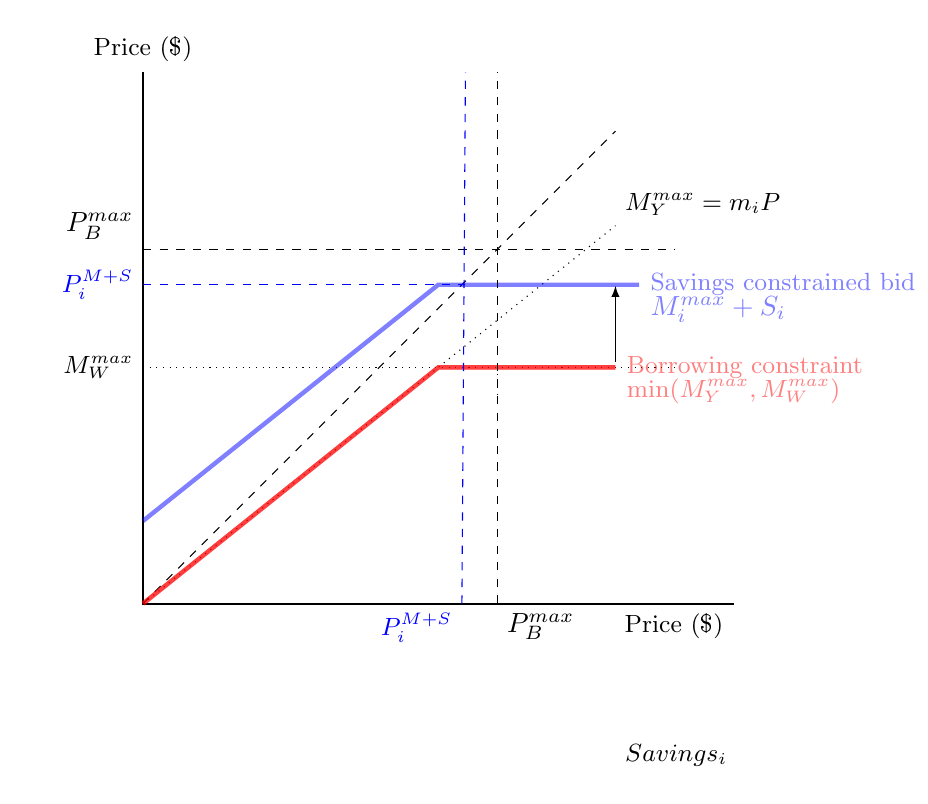
\begin{tikzpicture}	[scale=1.5]
%AXES
\draw[thick] (0,4.5)node[above]{\small Price (\$)} --(0,0)--(5,0)node[below left]{\small Price (\$)};
%\node at (-.25, 3.5)[ rotate=90]{\small Mortgage, Price (\$)};
% M =Mi MAX
\draw[dashed] (0,0)--(4,4);{node[right]}; %{\small $P$};
\draw[dotted] (0,2)node[left]{\small $M_W^{max}$}--(4.5,2);%node[right, red]{\small $M = M_i^{max}$};
% M =mi MAX
%\draw[dotted,red, opacity=.5] (0,0)--(4,3.6)node[right]{\small $M = 0.9P$};
\draw[dotted] (0,0)--(4,3.2)node[above right]{\small $M^{max}_Y = m_iP$};
% COMBINED MAX RED
\draw[ultra thick, red, opacity=.5] (0,0)--(2.5,2)--(4.0,2)node[right]{\small Borrowing constraint};
\draw[ultra thick, red, opacity=.5] (0,0)--(2.5,2)--(4.0,2)node[below right]{\small min($M_{Y}^{max},M_{W}^{max}$) };

\draw[ultra thick, blue, opacity=.5] (0,.7)--(2.5,2.7)--(4.2,2.7)node[right, ]{\small Savings constrained bid}node[below right, ]{$M_i^{max}+S_i$};
% SAVINGS
\draw[-latex] (4,2.05)node[below=5, right] {\small $Savings_i$}--(4,2.69);
% PMAX
\draw[dashed, ] (3,0)node[below right] {$P_B^{max}$}--(3,4.5);%node[, right]{\small desired max bid};
\draw[dashed,] (0,3)node[above left] {$P_B^{max}$}--(4.5,3);%node[, right]{\small desired max bid};

\draw[dashed, blue, thin] (2.7,0)node[below left] {\small $P_i^{M+S}$}--(2.73,4.5); %node[left, text width= 2cm]; %{\small };
\draw[blue, thin, dashed] (0,2.7)node[left] {\small $P_i^{M+S}$}--(2.73,2.7);%node[left, text width= 2cm]{\small savings constrained bid};
\draw[dotted ] (3,2)--(3,1.72);
\end{tikzpicture}
    \caption{Desired bid  and savings + mortgage constrained bid}
    \label{fig:savings-constraint}
    % I removed a line saying Savings sub i in lower corner
    \end{figure}

%
%If you are on the sloped line, constrained by $m$, the price is

% my version
% \begin{equation}
%     P_{B} \le min\Big(  min(m_i P_{B,i}^{max},\ M^{max}_i)+ S_i,\  P_{B,i}^{max}\Big)
% \end{equation}


% HOW DO WE COMPUTE DELTA? 
% \begin{lstlisting}
%     def get_discount_factor(self):
%         """
        
%         The discount factor gives the present value of one dollar received at particular point in the future, given the date of receipt and the discount rate.
%         Delta is the subjective individual discount rate for agent
%         after one year. This will be close to the prime interest rate, r_i.
%         """  
%         self.r_discount= .07
%         delta = 1/ self.r_discount
%         delta_period_1 = 1 / (1 + r_discount) 
%         delta_mortgage_period = delta_period_1**self.mortgage_period
%         #sum_delta = (1 - delta_mortgage_period)/delta
%         #return sum_delta
%         # sum_delta = delta_mortgage_period * (1 - delta_mortgage_period)
% \end{lstlisting}

\subsection{The bargaining model} \label{sec:bargaining-model}
Buyers place bids and a sale occurs if there is a surplus created by the transaction, that is if the the buyer's maximum bid exceeds owner's \gls{reservation price}, the maximum the owner would pay to retain their own property. 
Bargaining models attempt to identify the way the surplus available from a transaction is divided between the parties involved. Possible divisions are described by the red line in Figure~\ref{fig:Nash-bargaining-game}.\footnote{The classic  formulation by John Nash %\cite{Nash_John% (1953-01-01). "Two-Person Cooperative Games". Econometrica. 21 (1): 128–140. doi:10.2307/1906951. JSTOR 1906951, The Nash equilibrium: A perspective. Charles A. Holt and Alvin E. RothAuthors Info & Affiliations March 15, 2004 101 (12) 3999-4002 https://doi.org/10.1073/pnas.0308738101} 
identifies  `\gls{disagreement point},' which which is the  lowest value each player will accept. The combination of reservation price and maximum bid together are the disagreement point for a two-person price bargaining game. Since paying for the house is a negative for the buyer, the scale on the vertical axis  in Figure~\ref{fig:Nash-bargaining-game} is reversed to generate a version of the most common Nash bargaining figure.} 

    \begin{figure}
        \centering
        
  \begin{tikzpicture}[scale=1]
%  \draw [gray, opacity=.7] (0,0) grid (7,7);
\draw [<->] (0,6) node[above]{$buyer$}-- (0,0)node[left]{0}node[below]{0} -- (6,0) node[below]{$Seller$};
\draw [red, thick ] (1,7)--(7,1);
\draw [red, line width=1mm] (3,5)--(5,3);
\draw [red, thick, fill= yellow, opacity=.5] (3,3)--(3,5) -- (5,3)--cycle;

% vertical
\draw [blue, dashed] (0,5)node[left]{50,000}--(5,5)node[below right]{will not pay more}--(5,0)node[below]{50,000};
\draw [blue, ] (0,3)node[left]{30,000}--(6,3)node[above right]{can not get more};
% Horizontal
%\draw [blue, dashed] (4,0)--(4,6)node[above right]{will not accept less};
\draw [blue, ] (3,0)node[below]{30,000}--(3,6)node[above right]{can not offer less};
%\draw [ ultra thick] (0,0)--(1.5,1.5)node[ right]{equal set};
%\draw [dashed] (1,1) --(2,1)-- (2,0);
%\draw [red, ultra thick, dashed] (0,0) --(2.4,1.2)node[above]{relative equal set};
%\node at (2,1)[below right, ]{$(max\ u_1,\ max\ u_2)$};
%\node at (3.5,3){Agreement set};\node at (3,3.5){\Large A};

\node at (3,3)[below left, text width=2.8cm, align=right]{\textbf{disagreement\newline point}};
\node[mark size=4pt,color=red] at (3,3) {\pgfuseplotmark{square*}};

\end {tikzpicture}


        \caption{The Nash bargaining game}
        \label{fig:Nash-bargaining-game}
    \end{figure}


In Figure~\ref{fig:Nash-bargaining-game} we imagine the seller values the property at \$30,000 (the reservation price) and the buyer values it at \$50,000 (the maximum bid price).  At any price above \$30,000 the seller is better off. At any price below \$50,000 (above -\$50,000 on the vertical axis) the buyer is better off. 
The set of acceptable bargains acceptable to both is above and to the right of the point labeled `disagreement point.' 

In principle the buyer could pay more than \$50,000 or the seller could accept a price below \$30,000, but neither would do so if they are rational. 
The thick red line segment, called the bargaining set, represents all the outcomes that are\begin{enumerate}
    \item Efficient, because the entire \$20,000 surplus is allocated to the players. 
    \item Feasible, because the players involved gain no more in total than the potential increase in value generated by the transaction.
    \item Rational because neither player has to accept an outcome that makes them worse off.
\end{enumerate}   

The bargaining processes will ideally lead to a point on that thick red line segment. In practice, some of the surplus is dissipated in the sale process, and some is absorbed by intermediaries. We ignore this refinement for the current version of the model. Differences in relative power will tip the outcome in favour of the stronger player.   Players who can afford to wait will get a larger share of the gain. Excess demand favours sellers. Low vacancy rates favour owners over tenants.   If there is a deal, it will still be at a price between the maximum bid and the reservation price, and in most cases probably somewhere near the midpoint. Sellers might reduce the asking price if the home fails to sell in the first period it is on the market.\footnote{Uncertainty adds further complications. Parties may not know each other's disagreement point. PartieS post asking prices greater than their reservation price or initial offers much lower than their true valuation.  
Negotiations often proceed through a series of offers and counteroffers.}\;\footnote{In an overheated housing market bid prices might exceed asking prices, but the price won't exceed the maximum expected profitable bid price, $P_B^{max*}$. We could elaborate the model by defining a measure of \gls{sellers' bargaining power} based on vacancies and expected prices.}   % Ariel Rubinstein \cite{rubinsteinPerfectEquilibriumBargaining1982} presented a convincing solution to the alternating offers model in a 1982 paper. His process converges to the Nash solution. 
% }
%  The higher asking price and lower bids are `cheap talk' (In game theory, cheap talk is communication between players that does not directly affect the payoffs of the game. % This is in contrast to signaling in which sending certain messages may be =


 


% \subsubsection{Maximum bids}
% The rate of return calculation in  Equation~\ref{eqn-property-investment-return1} combined with the investment criterion in Equation~\ref{eqn-property-investment-return2} identifies the maximum  that price that an investor can price offer for a property  and still maker sa profit.

% \begin{align}
% %r^{target}& \le \frac{\delta^\mathbb{T}}{1-m} \left(\dot P_\mathbb{T} - (1+r)^\mathbb{T})m  + \frac{\mathcal{R}_{N, \mathbb{T}}}{P_B^{max}}\right)\nonumber\\
% % (1-m)r^{target}/\delta^\mathbb{T} &\le \dot P_\mathbb{T} - (1+r)^\mathbb{T}m  +   \frac{\mathcal{R}_{N, \mathbb{T}}}{P_B^{max}} \\
% % (1-m)r^{target}/\delta^\mathbb{T} - \dot P_\mathbb{T} + (1+r)^\mathbb{T}m &\le  \frac{\mathcal{R}_{N, \mathbb{T}}}{P_B^{max}}\nonumber\\
% P_B^{max} &\le  \frac{\mathcal{R}_{N, \mathbb{T}}}{(1-m)r^{target}/\delta^\mathbb{T} - \dot P_\mathbb{T} + (1+r)^\mathbb{T}m} \label{eqn:maximum-bid}
% \end{align}

% We call this  $i's$ maximum bid.
% .\footnote{The denominator in Equation~\ref{eqn:maximum-bid} can be seen as an adjusted rate of return for capitalizing net rents, analogous to the value of $r$ in  the standard capitalization formula.} 
% It represents the value of the stream of rent plus any capital gains, and is therefore the most reasonable reservation price for sellers as well the most reasonable maximum offer for potential buyers. In principle it exists for all potential buyers and sellers for every property. In practice, only a subset of potential buyers and sellers are in the market at any time. 




\subsection{The many-to-one matching problem}
\textbf{The housing market is usually a many-to-many matching problem}: which property goes to which buyer? For each property that comes on the market, there will be a set of potential buyers with differing maximum bids. Some simplifications are available. In each sale, the bidder with the highest bid price among those currently bidding on that property will make the purchase.\footnote{For many reasons the process is likely to exhibit a good deal of randomness and inefficiency. For our purpose, the general messiness of the market is unlikely to do more than slow and blur results somewhat.} Since the highest bidder is competing with the second-highest bidder, we expect the final price to be equal to the second-highest maximum bid, shown as the star in figure~\ref{fig:auction-game}. 


    \begin{figure}
        \centering
        
\begin{tikzpicture}[scale=1]
%  \draw [gray, opacity=.7] (0,0) grid (7,7);
\draw [<->] (0,8.25) node[left, text width=1cm]{Buyer pays}-- (0,0)node[left]{0}node[below]{0} -- (8.25,0) node[below right, text width=1cm]{Seller gets};
\draw [red, thick, latex-latex ](1.5,5.5)node[below left, black, text width=1cm]{Feasible\\ set}-- (2,6)--(6.5,1.5)--(6,1);
\draw [red, line width=1mm] (3,5)--(5,3);
\draw [red, thick, fill= yellow, opacity=.5] (3,3)--(3,5) -- (5,3)--cycle;

% % vertical axis
\draw [dashed] (0,5) node[left] {-\$30,000} -- (3,5) ;
\draw [dashed] (0,3) node[left] {-\$50,000} -- (5.5,3) ;
\draw [dashed] (3,0) node[below]{ \$30,000} -- (3,5.5) ;
\draw [dashed] (5,0) node[below]{ \$50,000} -- (5,3) ;
\draw [dashed, thick, blue] (0,2) node[left] {-\$60,000} -- (7,2)
node [right,text width=2cm]{highest bid};

%  \draw[pattern=north west lines, distance=2mm,pattern color=red!30, draw=none] (0,0) rectangle (3,8);
%  \node[text width=2.5cm] at (1.5,7) {\small Seller will not accept less than \$30,000};

% \draw[pattern=north east lines, pattern color=green!60, draw=none] (0,0) rectangle (9,3);
% \node[text width=2.5cm]at (7,1.5)  {\small Buyer will not pay more than \$50,000};

\draw [ latex-latex, ultra thick](3.7,7)-- (3,7)--(3,3)--(7,3)node[right,text width=2cm]{second highest bid}--(7,3.7)node[above ]{Rational Set} ;
\draw [ latex-, thick, red](3.5,4.5)-- (4,5)--(5.5,5)node[right]{Bargaining Set} ;

\draw [ latex-, thick, red](2.5,5.5)-- (3.6,6.5)--(5.5,6.5)node[right]{Efficient Set} ;%name

%\draw [ latex-, thick, red](3.5,4.5)-- (4,5)--(5.5,5)node[right]{Bargaining Set} ;

%\draw [dashed] (1,1) --(2,1)-- (2,0);
%\draw [red, ultra thick,3 dashed] (0,0) --(2.4,1.2)node[above]{relative equal set};
%\node at (2,1)[below right, ]{$(max\ u_1,\ max\ u_2)$};
%\node at (3.5,3){Agreement set};\node at (3,3.5){\Large A};

\node at (3,3)[left, text width=1.8cm, align=right]{\textbf{\tiny Disagreement\newline point}};

\node[mark size=4pt,color=red] at (3,3) 
{\pgfuseplotmark{square*}};

\node[mark size=8pt,color=blue] at (5,3) 
{\pgfuseplotmark{10-pointed star}};

\draw;
\end {tikzpicture}
        \caption{Auction with a second, higher bid}
        \label{fig:auction-game}
    \end{figure}

%.\footnote{We could allow potential buyers  to approach potential sellers who have not listed with an offer and allow worker-owners to consider retiring early or becoming tenants if an offer is attractive.  This is only likely if speculative pressures are strong. It may require having multiple institutional buyers to make offers more competitive. In that case, initial offers will be closer to the maximum bid price, tending to pull prices up and benefit potential sellers.}  
When there is one bidder, we will employ a simple rule for splitting the gain from trade. Both simplifications are grounded in standard bargaining theory.



\subsection{The bargaining process}
We have now identified a set of bids and a reservation price for each property on the market that must be converted to a price for that property using the bargaining rule. 
The bargaining  mechanism then simply has to compare the maximum bid price $P_B$ with the seller's reservation price. If the $P_B^{max}>P_R$, a deal that is between the two values is possible. Otherwise, the transaction does not proceed.
If a bargain is possible, the rule is simple: 
\begin{enumerate}
    \item If there is only one maximum bid above the reservation price, split the difference between the bid and the reservation price evenly.\footnote{It is fairly simple if perhaps not very revealing to incorporate relative power as described in Footnote~\ref{fn:relative-power}.} If $P_B^{max}>P_R$,  the bargaining rule selects a value 
    \[P = xP_B^{max}+(1-x)P_R, \ \ \ x\in [0\dots 1] \]
where $x$ is typically 0.5.
    \item If there are two or more maximum bids above the reservation price, the property goes to the highest and since the bids are the maximum the buyers would pay under any circumstances, the price is set a the second highest bid in order to reflect the tightness of the market.\footnote{This is an application of Vickrey \gls{second-price auction} theory\cite{levinAuctionTheory2004}.} 

\end{enumerate}
  
    \begin{figure}[!thb]
    \centering
    \begin{tikzpicture}
%\draw[step=0.5cm,color=gray] (0,-3) grid (8,7);
\node [above](Bank)at (1,7) {Bank};
\node [above](Buyers)at (5,7) {Buyers $i$};
\node [above](Seller)at (7,7) {Seller};

\draw[ultra thick, -latex](Bank)--++(0,-1.5)node[below]{$P_B^{max}$};
\draw[ultra thick, -latex](Buyers)--++(0,-1.5)node[below]{$P_i^{max}$};
\draw[ultra thick, blue!60,-latex](Seller)--++(0,-1.5)node[below]{$P_R$};

\node[above, red, text width=1.55cm, align=center]at (3,5){Select two highest bids};

\begin{scope}[shift={(0,-1)}]
\draw[ultra thick](1,6.)--(5,6.0); % Bar
\draw[ultra thick, blue!60,-latex](7,6.2)--++(0,-1)--++(-4,0)node[left, red]{Compare};  %Pass P_R to if-then
\draw[ultra thick, -latex](3,6)--++(0,-1.5)--++(-2.,-.5);% down and left
\draw[ultra thick, -latex](3,5)--++(0,-1)node[below, text width=1.5cm, align=center]{none above {$P_R$} };%
\draw[ultra thick, -latex](3,5)--++(0,-.5)--++(2.2,-.5)node[below, text width=1.cm, align=center]{One above {$P_R$} };
% down and Right

\draw[ultra thick, -latex](.1,2.5)node[above, text width=2.cm, align=center]{two or more above {$P_R$} }--++(0,-.75)node[below, text width=3cm, align=center]{Auction: price is second highest $P_i^{max}$, house goes to highest bidder};

\draw[ultra thick, -latex](3,2.5)--++(0,-.75)node[below, text width=2cm, align=center]{No sale};

\draw[ultra thick, -latex](5.5,2.5)--++(0,-.75)node[below, text width=2cm, align=center]{Bargain: price is power-modified mean};
\end{scope}

\end{tikzpicture}
    \caption{The Bargaining model and price determination}
    \label{fig:Bargaining}
    \end{figure}


% \[P^{ask}>P_M^e> 0.95 P^r\]
% Otherwise
% \[P^{ask}> 1.10P^r>P_M^e\]
% If no offer exceeds the reservation price, no sale is made.

% Once an owner reached retirement age, if no sale is made the reservation price is reduced for the next cycle.
% If no sale is made the owner considers becoming a landlord. if the present value of net rent is above the reservation price, the owner rents out the home. 



{\color{red}
\section{OOD documentation of the agent based model}

THIS PART IS NEW AND VERY ROUGH

MAYBE ADD A NOTE ON METHOD, INTRODUCE ABM AND HOW IT RELATES WITH EQUATION BASED MODELLING

The core model is documented bellow using the Overview, Design concepts, and Details (OOD) standard. It includes the seven elements: purpose, state variables and scales, process overview and scheduling, design concepts, initialization, input, and submodels.

\subsection{Purpose}

The purpose of this model is to understand ..
Following xyz, xyz gives x purposes for modelling. The purpose of this model is xyz. It is to understand financialization of the urban housing market. 


\subsection{State variables and scales}

The agents are workers,  %  who may choose to work at an urban firm, properties, each occupying a an urban grid space. %, 
the urban firm, an investor, a bank, and a realtor. People live in residences, have ages, savings and mortgages, can own property and can choose to work or not work in the city, depending on wages and transportation costs. Properties have owners, residents, and locations. Firm have sizes, marginal returns to capital, and labour ..., 
Investors own properties and take out debt, the bank has lending rates that are a function of their calculation of credit-worthyness and the prime interest rate, and realtors have lists of propertys for sale and for rent. 

Each agent occupies one property, however the firm has a density parameter which multiplies the firm population by a density number, effectively coarse grainning the model for the purposes of the firms calculation.

Each time step represents one year. People work until they reach retirment age at which point they retire. 
% There are x types of agents. They have the state variables outlined in the tables. 

% variables can include behavioral attributes and model parameters.
the model’s entities, their state variables (possibly including behavioral attributes and model parameters), and the model’s spatial and temporal scales.

Environment variables include XXX

Overview of process, parameters and defaul values for the xx model

\subsection{Process overview and scheduling}

Each time step represents one year. The model proceeds with discrete steps. All agents of a particular time execute their step function in randomized order. They sequence of the code means they do not use information from, or interact with agents of the same type during their step function, so the order doesn't matter. In each time step first the firm computes the wage, land units calculate their warranted prices based on the firm's urban wage premium. If people are above the retirement age, they retire, and list any properties for sale if they are moving out of the city. Those not retired choose whether to work or not work, based on the wage premium and transportation costs. Next newcomers and investors bid on properties listed for sale. Realtors take the list of all bids and select the top bids and facilitate a bargaining process to reach a final price. Finally, if the owners will not occupy their own houses, properties are listed for sale and rented to newcomers, and the process begins again in the next time step. 

% Overview of process, parameters and default values for the xx model
% - description of the model’s schedule that is detailed and precise enough to allow the model to be re-implemented.
% - schedule descriptions based on pseudo-code most useful.


\subsection{Design concepts}

Basic principles
Adaptation - adaptive traits - rules for  how changing in response to changes in environment or themselves. do they seek to increase some measure
Objectives - what is the objective and how is it measured
No - Learning - change adaptive traits based on experience
Prediction - the anticipate based on past prices





Basic principles explored include the relationship between urban agglomeration effects and financialization of the the urban housing market. The model also expresses several other concepts as described below.

\subsubsection{Emergence}
There are two distinct regimes one in which investors own properties. Given the feedbacks, there is a regime in which wealth grows and one in which it collapse, there is a regime in which those who own houses and work can build equity and live comfortably and one in which they are continually squeezed by costs. This emerges as a by product of individual investment based on local expected financial return calculations. 
The expected price includes information about how the market has behaved so it is possible for price bubbles and expectations to feed back into the dynamics. 

Ownership, the regime, emerges, advantage are amplified leading to a different end state.

\subsubsection{Adaptation, learning and prediction}

TODO add adaptive traits - rules for how changing in response to changes in environment or themselves. do they seek to increase some measure

Objectives - what is the objective and how is it measured
the objective is profit

There is not learning in the sense that they do not change their adaptive traits based on experience. 


There is some prediction, in that bidders anticipate prices based on the rate at which those prices have increased in the past $\dot P$.


\subsubsection{Sensing}
All agents have information about the wage, warranted price, expected and their own borrowing costs. They make their decisions based on what is best for them. 

\subsubsection{Interaction}
Agents get information from the firm about wages. The independently make decisions to work or retire, but because of agglomeration effects, their decision to work and it's effect on the size of the labour market feed back to effect wages in the next step. 

\subsubsection{Stochasticity}
Stochasticity comes into the main model through the range of initial agents and savings. For model sensitivity analysis, we use a simple submodel that calculates relative bids, and shortcuts the land market and bidding process so we can see the effects of parameter changes without stochasticity. 

\subsubsection{Feedback loops}
Feedback loops are not part of the ODD standard, but an important concept in this work. 
% https://en.wikipedia.org/wiki/James_J._Kay
% https://www.researchgate.net/scientific-contributions/James-J-Kay-2162967174
% https://uwaterloo.ca/systems-design-engineering/about-systems-design-engineering/department-history
There are two main \glspl{feedback loop} in the model: the productivity-wage, population-productivity loop that we call the Alonso-Jacobs cycle, and the speculative investment-price, inflation-investment cycle that may produce price bubbles. 
% Our model incorporates two important feedback loops. One, driven by agglomeration, we call the \Gls{Alonzo-Jacobs cycle}. The other is a price-financialization feedback that directly changes the ownership pattern in the urban housing market. 
The two loops are linked. One mechanism is that rising productivity raises wages which then works through two paths. It can raise rents, effectively transferring productivity gains to landowners, or it can draw more workers, enhancing the \Gls{Alonzo-Jacobs cycle}. 

A rapid increase in housing prices may choke off urban population growth and cause the \Gls{Alonzo-Jacobs cycle} to stall. Rapid expansion of the housing stock should have the opposite effect. Much depends on the speed of response of the housing stock and the rate of transmission of agglomeration effects to wages. Our base model allows the housing stock to respond instantly and automatically increments the wage with a small lag. In the base model, financial flows are unrestricted but the rate of financialization is limited by the rate of turnover of ownership. We then parameterize the rate of adjustment for each of the stocks in a simple way in order to conduct sensitivity analysis.

Feedback loops are a fundamental feature of almost all systems. They have probably been recognized by theorists for centuries. Marx, to take one relatively modern example, identified the growth dynamic of the capitalist system  as a feedback loop, with capital investments producing a surplus that was fed back into investment, growing the stock of capital. He  claimed that this loop produced dynamic instability and a great deal of subsequent work has supported his insight \cite{dumenilStabilityInstabilityDynamic1986}.\cite{schumpeterInstabilityCapitalism1928}. More recently, the Keynesian multiplier is a result of feedback in macro models between expenditure and income. That loop produces a stable equilibrium. Neoclassical growth theory built on that mechanism to explore the determinants of economic growth using differential and difference equations. Forrester, the creator of system dynamics computer simulation modeling, argued that change over time is caused by the process of accumulation.

The feedback concept formally entered the social sciences through two channels: cybernetics, pioneered by Nobert Wiener  and the participants of the Macy Foundation Conferences, and the servomechanism/control engineering thread championed by Jay W. Forrester and others. Both threads were picked up and applied by prominent economists. \footnote{Richardson \cite{richardsonFeedbackThoughtSocial1991} mentions Oscar Lange (1970), Kenneth Boulding, and Alfred Eichner, Phillips,  R. G. D. Allen (1956), and Axel Leijonhufvud.} There is now a niche sub-discipline in economics called ``Feedback Economics'' \cite{radzickiIntroductionFeedbackEconomics, cavanaFeedbackEconomicsEconomic2021}. %  and a great deal of work in The servomechanism/control engineering thread is the one most closely related to \gls{system dynamics} modeling and to ideas used in this thesis.



\subsubsection{Observation}
The model records the urban wage, bid prices, realized price, population, which people worked and who owned what properties.

\subsection{Initialization}
Initial values for the model are

\subsection{Input}
To explore the model dynamics interventions change key parameters mid run. XYZ

to represent time varrying data. 

\subsection{Submodels}
Three submodels are the spatial structure of the model, with each land unit having a transportation cost based on its distance from the urban center, second the firm model that produces the urban wage, and finally the land market model that allows homeowners and financialized investors to bid on properties in order to capture the rising rents due to agglomeration.  
}
\chapter{Model Characterization} \label{chapter-characterization}   %%% NO

\chapter{Ownership} \label{chapter-ownership}

The two main hypotheses of this thesis are, first,  that the financial sector affects the ownership of housing and the class structure of society, and second that this may have implications for urban productivity. We begin with the first hypothesis. The section of the model that we call the produces demand for land. In the housing market section land agents bid for land. competition between would-be owner-occupiers and investors results in an evolving allocation of ownership of land. The ownership pattern determines the distribution of the locational rents generated by the city.

\begin{figure}
\centering
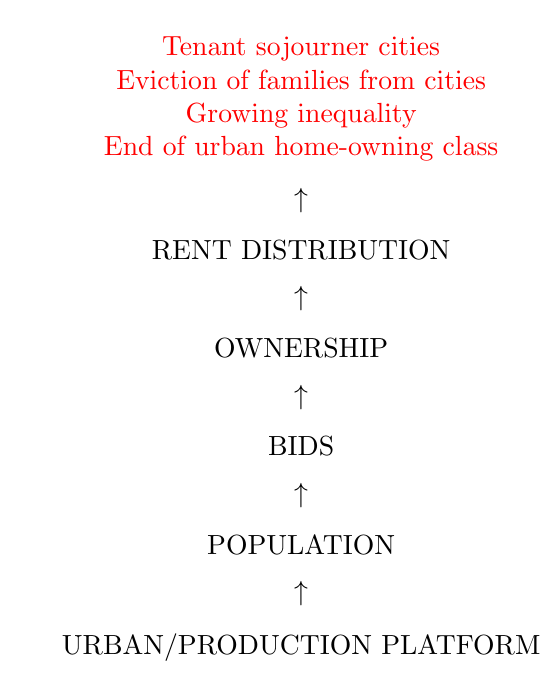
\begin{tikzpicture}
  \node at (0,0) (1) {URBAN/PRODUCTION PLATFORM};
   \node[above=1mm of 1] (A1) {$\uparrow$};
   \node[above=1mm of A1] (Pop) {POPULATION};
   \node[above=1mm of Pop] (APop) {$\uparrow$};
   \node[above=1mm of APop]  (3) {BIDS};
   \node[above=1mm of 3] (4) {$\uparrow$};
   \node[above=1mm of 4] (5) {OWNERSHIP};
   \node[above=1mm of 5] (6) {$\uparrow$};
   \node[above=1mm of 6] (7) {RENT DISTRIBUTION};
   \node[above=1mm of 7] (ARent) {$\uparrow$};
    \node [above=1mm of ARent, text width= 6cm, text centered, red] {Tenant sojourner cities\\ Eviction of families from cities\\Growing inequality\\ End of urban home-owning class};
   % \node[above=1mm of 1] (2) {$\uparrow$};
   % \node[above=1mm of 2] (3) {Growing inequality};
   % \node[above=1mm of 3] (4) {$\uparrow$};
   % \node[above=1mm of 4] (5) {Eviction of families from cities};
   % \node[above=1mm of 5] (6) {$\uparrow$};
   % \node[above=1mm of 6] (7) {Tenant sojourner cities};
\end{tikzpicture}
\caption{TODO}
\label{fig:enter-label}
\end{figure}

The interlinked social consequences of any shift from owner-occupancy to tenancy, shown in red, are dramatic. 

%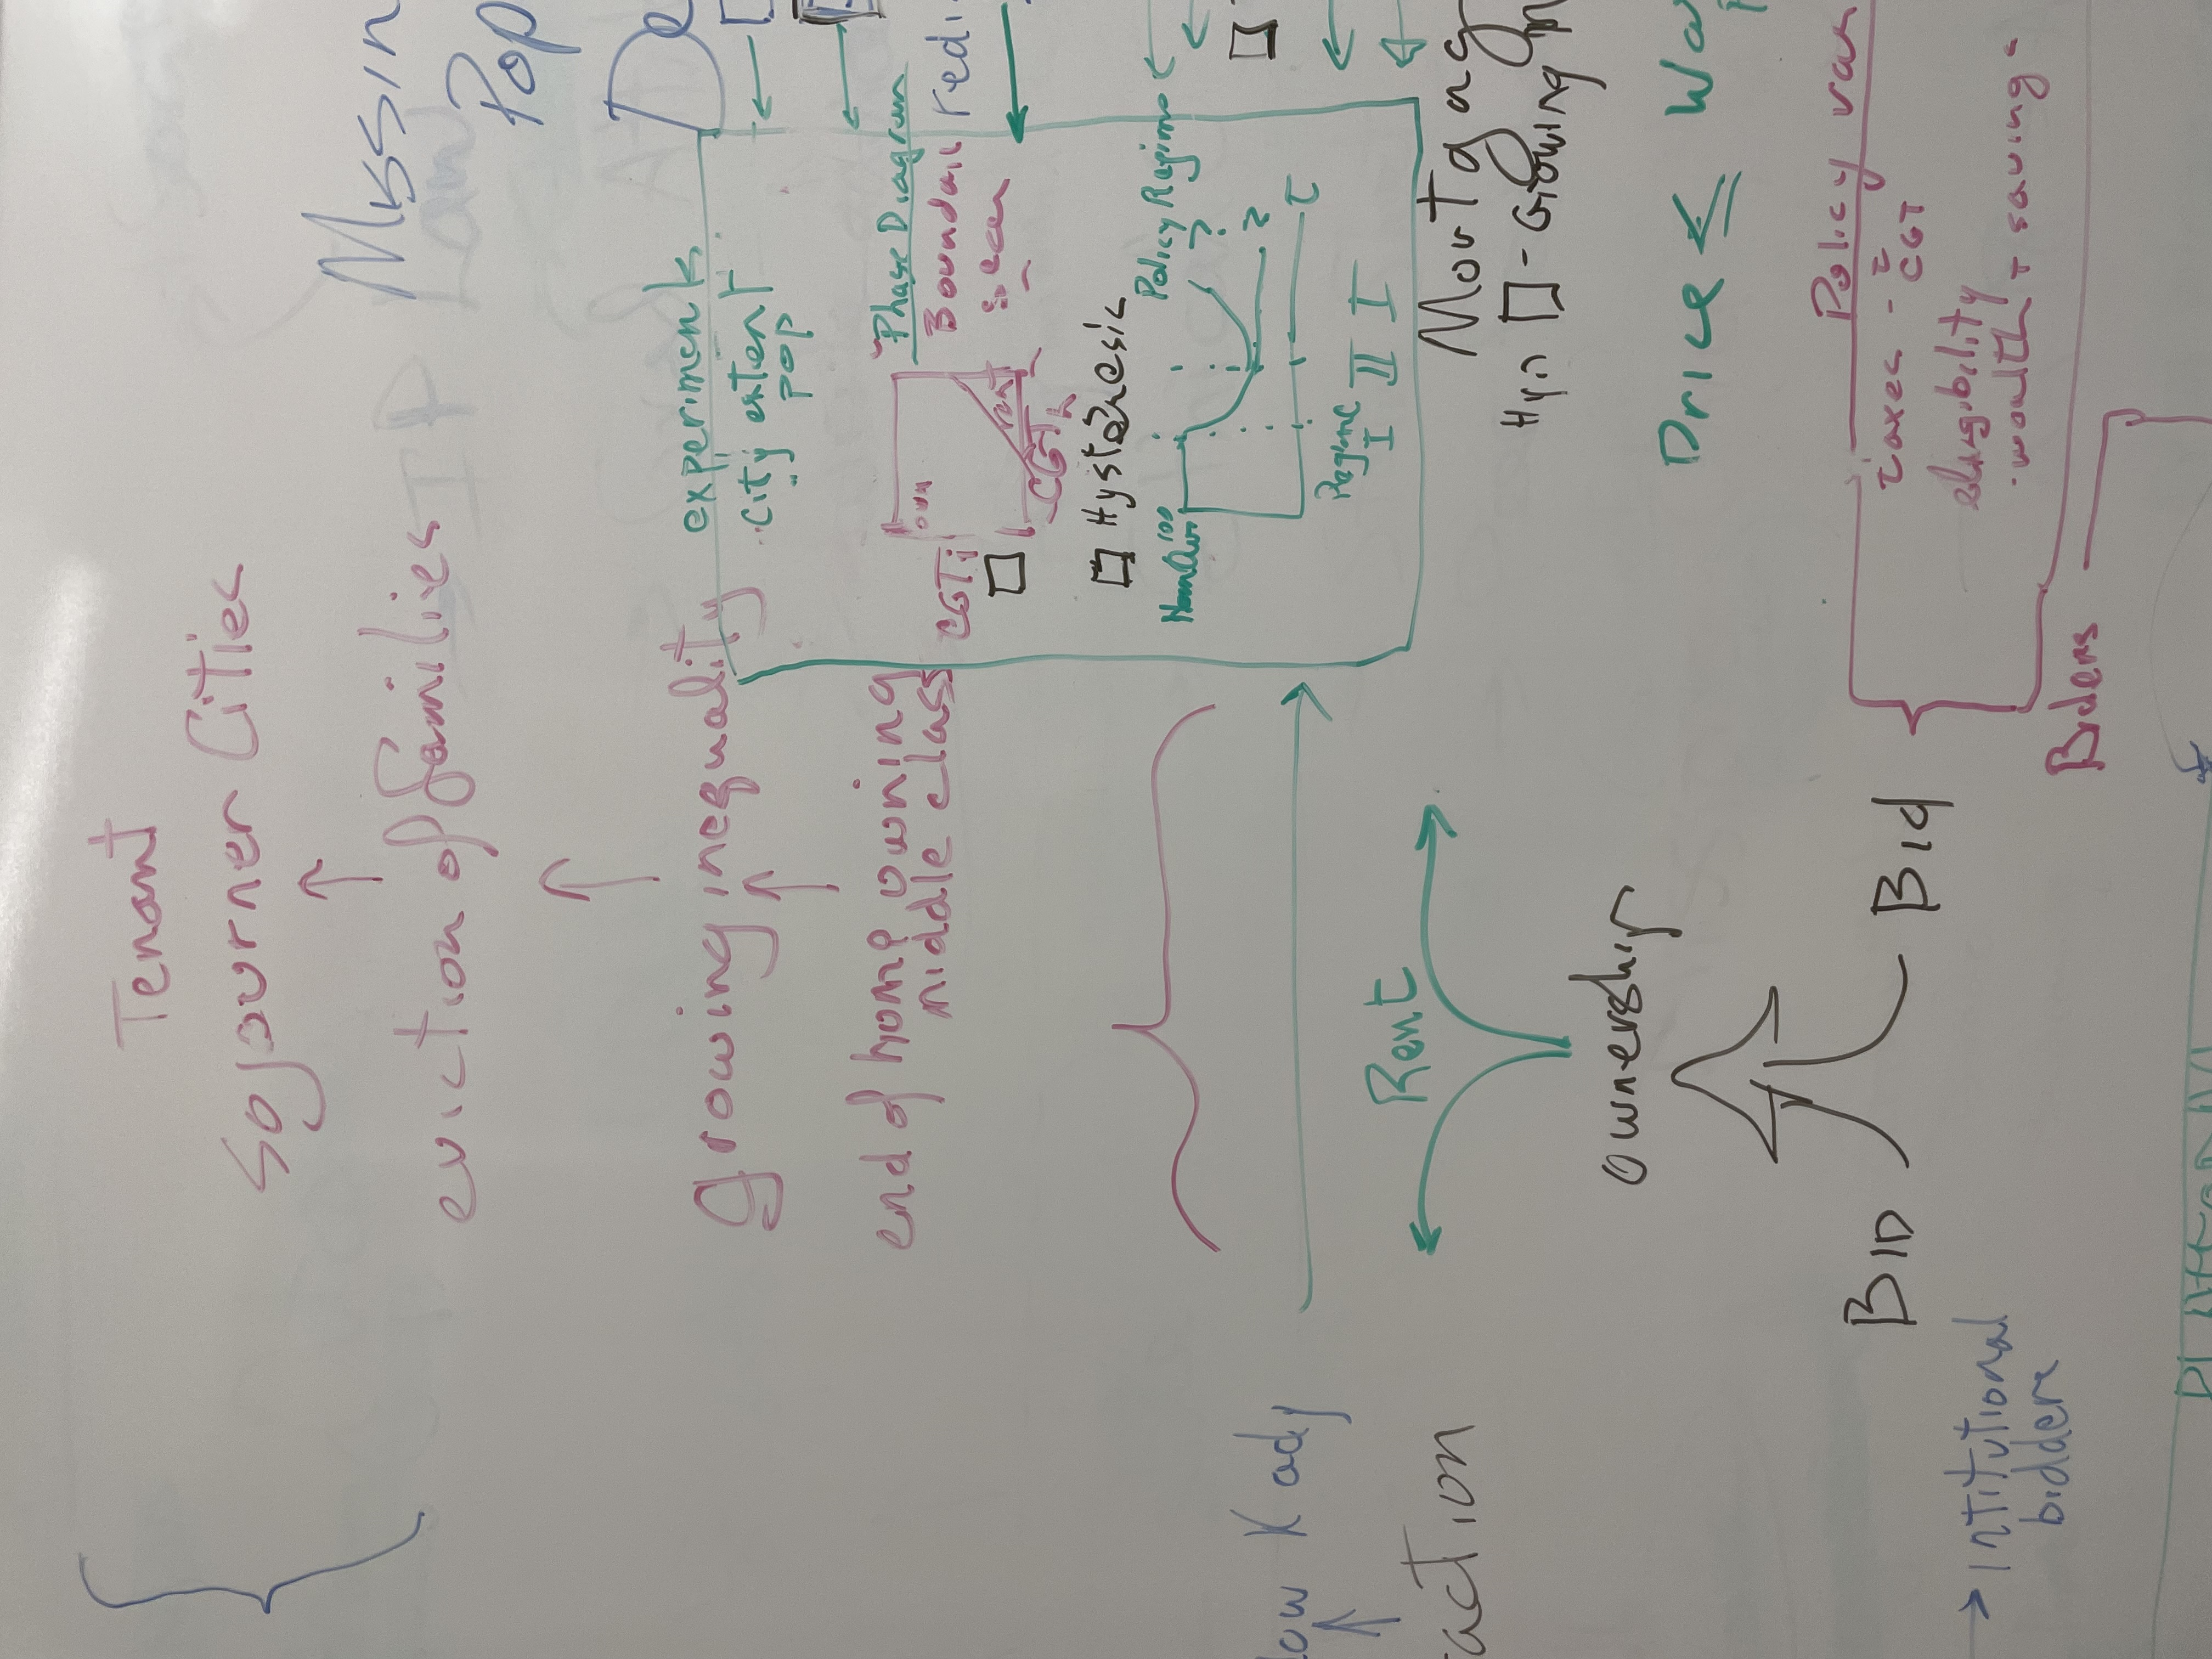
\includegraphics[scale=.5, angle=-90]{fig/IMG_2691.jpg}

We are observing these processes underway in the real world. We need to know if they are explained by a theoretically-consistent model of the urban economy that incorporates the financialization process.

\section{Ownership of housing}

With certain plausible parameter settings our baseline model, produces an evolutionary trajectory of class ownership of housing similar to that illustrated in Figure ~\ref{fig:Baseline_ownership_trajectory}. The distribution of ownership then determines the distribution of the locational land rents, which are the product of agglomeration effects. 

Recall that our first hypothesis is that in and \Gls{Alonzo-Jacobs model}, the financial sector will tend to take over a growing share of property ownership within a city. Figure ~\ref{fig:Baseline_ownership_trajectory} shows an initial situation with close to 100 owner-occupiers and a small number of investor-owners. Although the number of owner-occupiers grows in the initial period in Figure ~\ref{fig:Baseline_ownership_trajectory}, over time financial capital acquires an increasing share of the housing stock. By the time the city reaches its maximum size, the city has been transformed from a city of homeowners to a city of tenants.

DISCUSS THE PARAMETERS THAT AFFECT OWNERSHIP? We have conducted parameter sweeps to identify policy parameters that can affect the distribution of ownership.

\begin{figure}
    \centering
    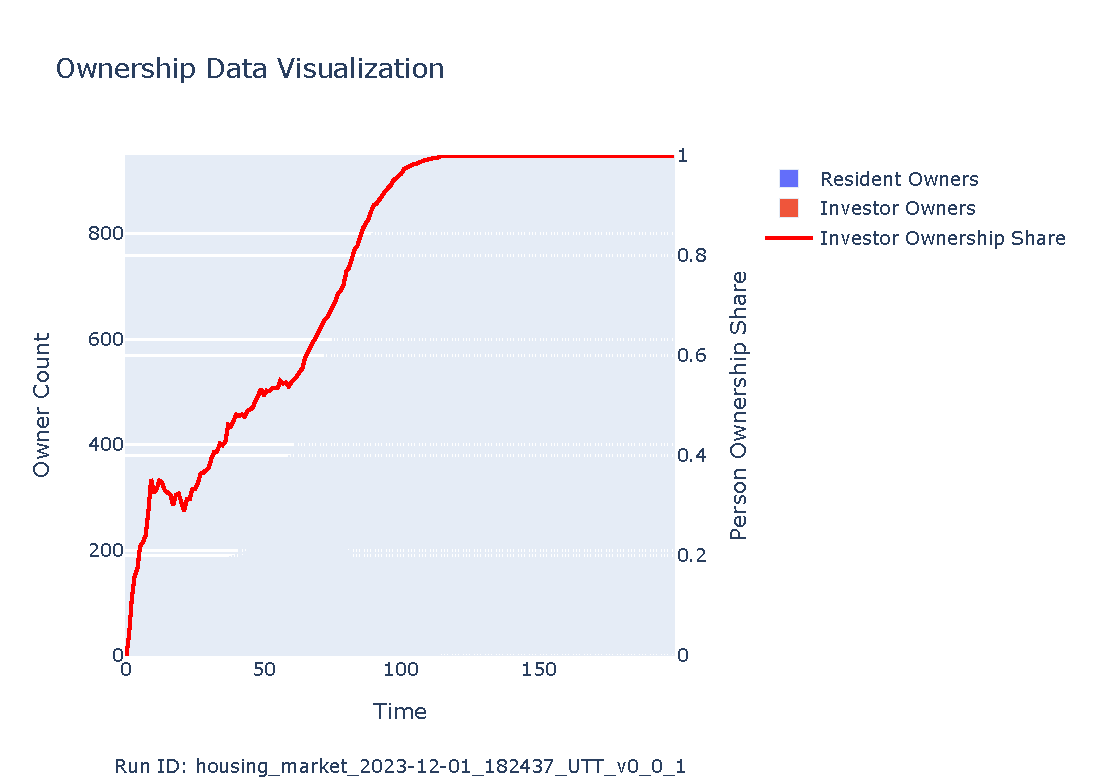
\includegraphics[scale=.8, trim={0 1cm 0 1.8cm},clip]{fig/Analysis/Ownership_Data_1.pdf}
    \caption{The transformation from a city of homeowners to a city of tenants in the baseline model}
    \label{fig:Baseline_ownership_trajectory}
\end{figure}

%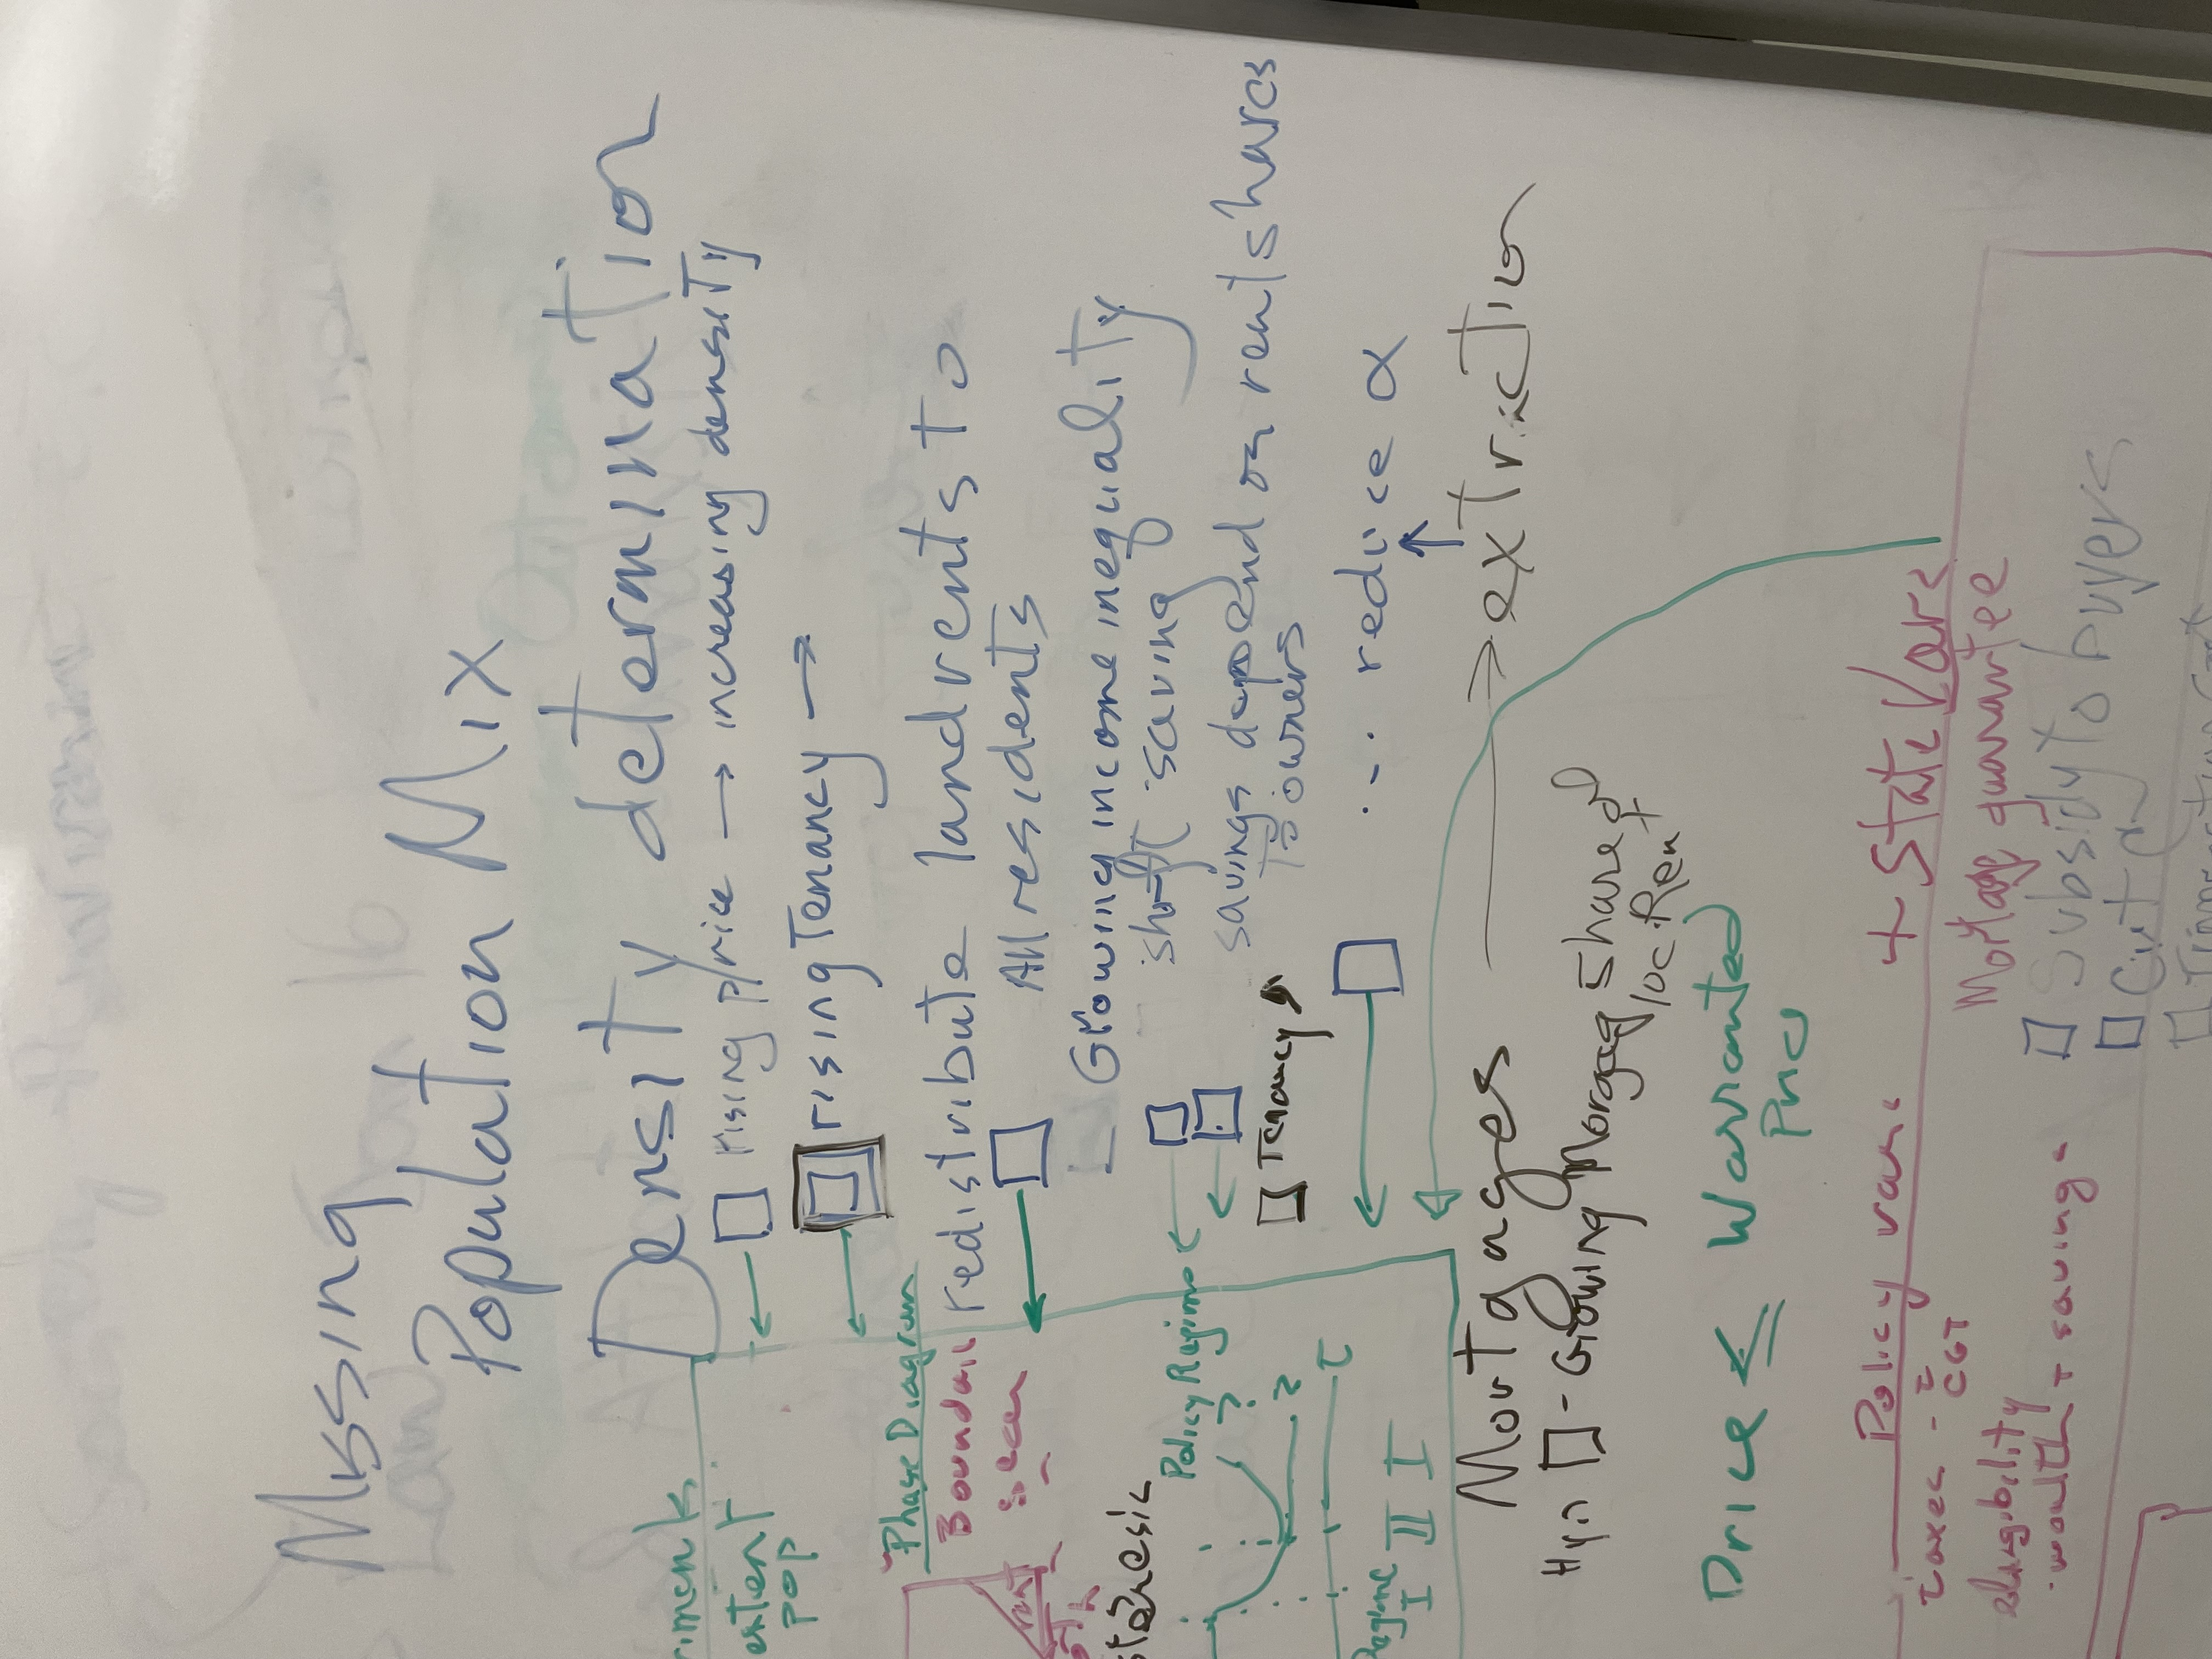
\includegraphics[scale=.5, angle=-90]{fig/IMG_2688.jpg}


%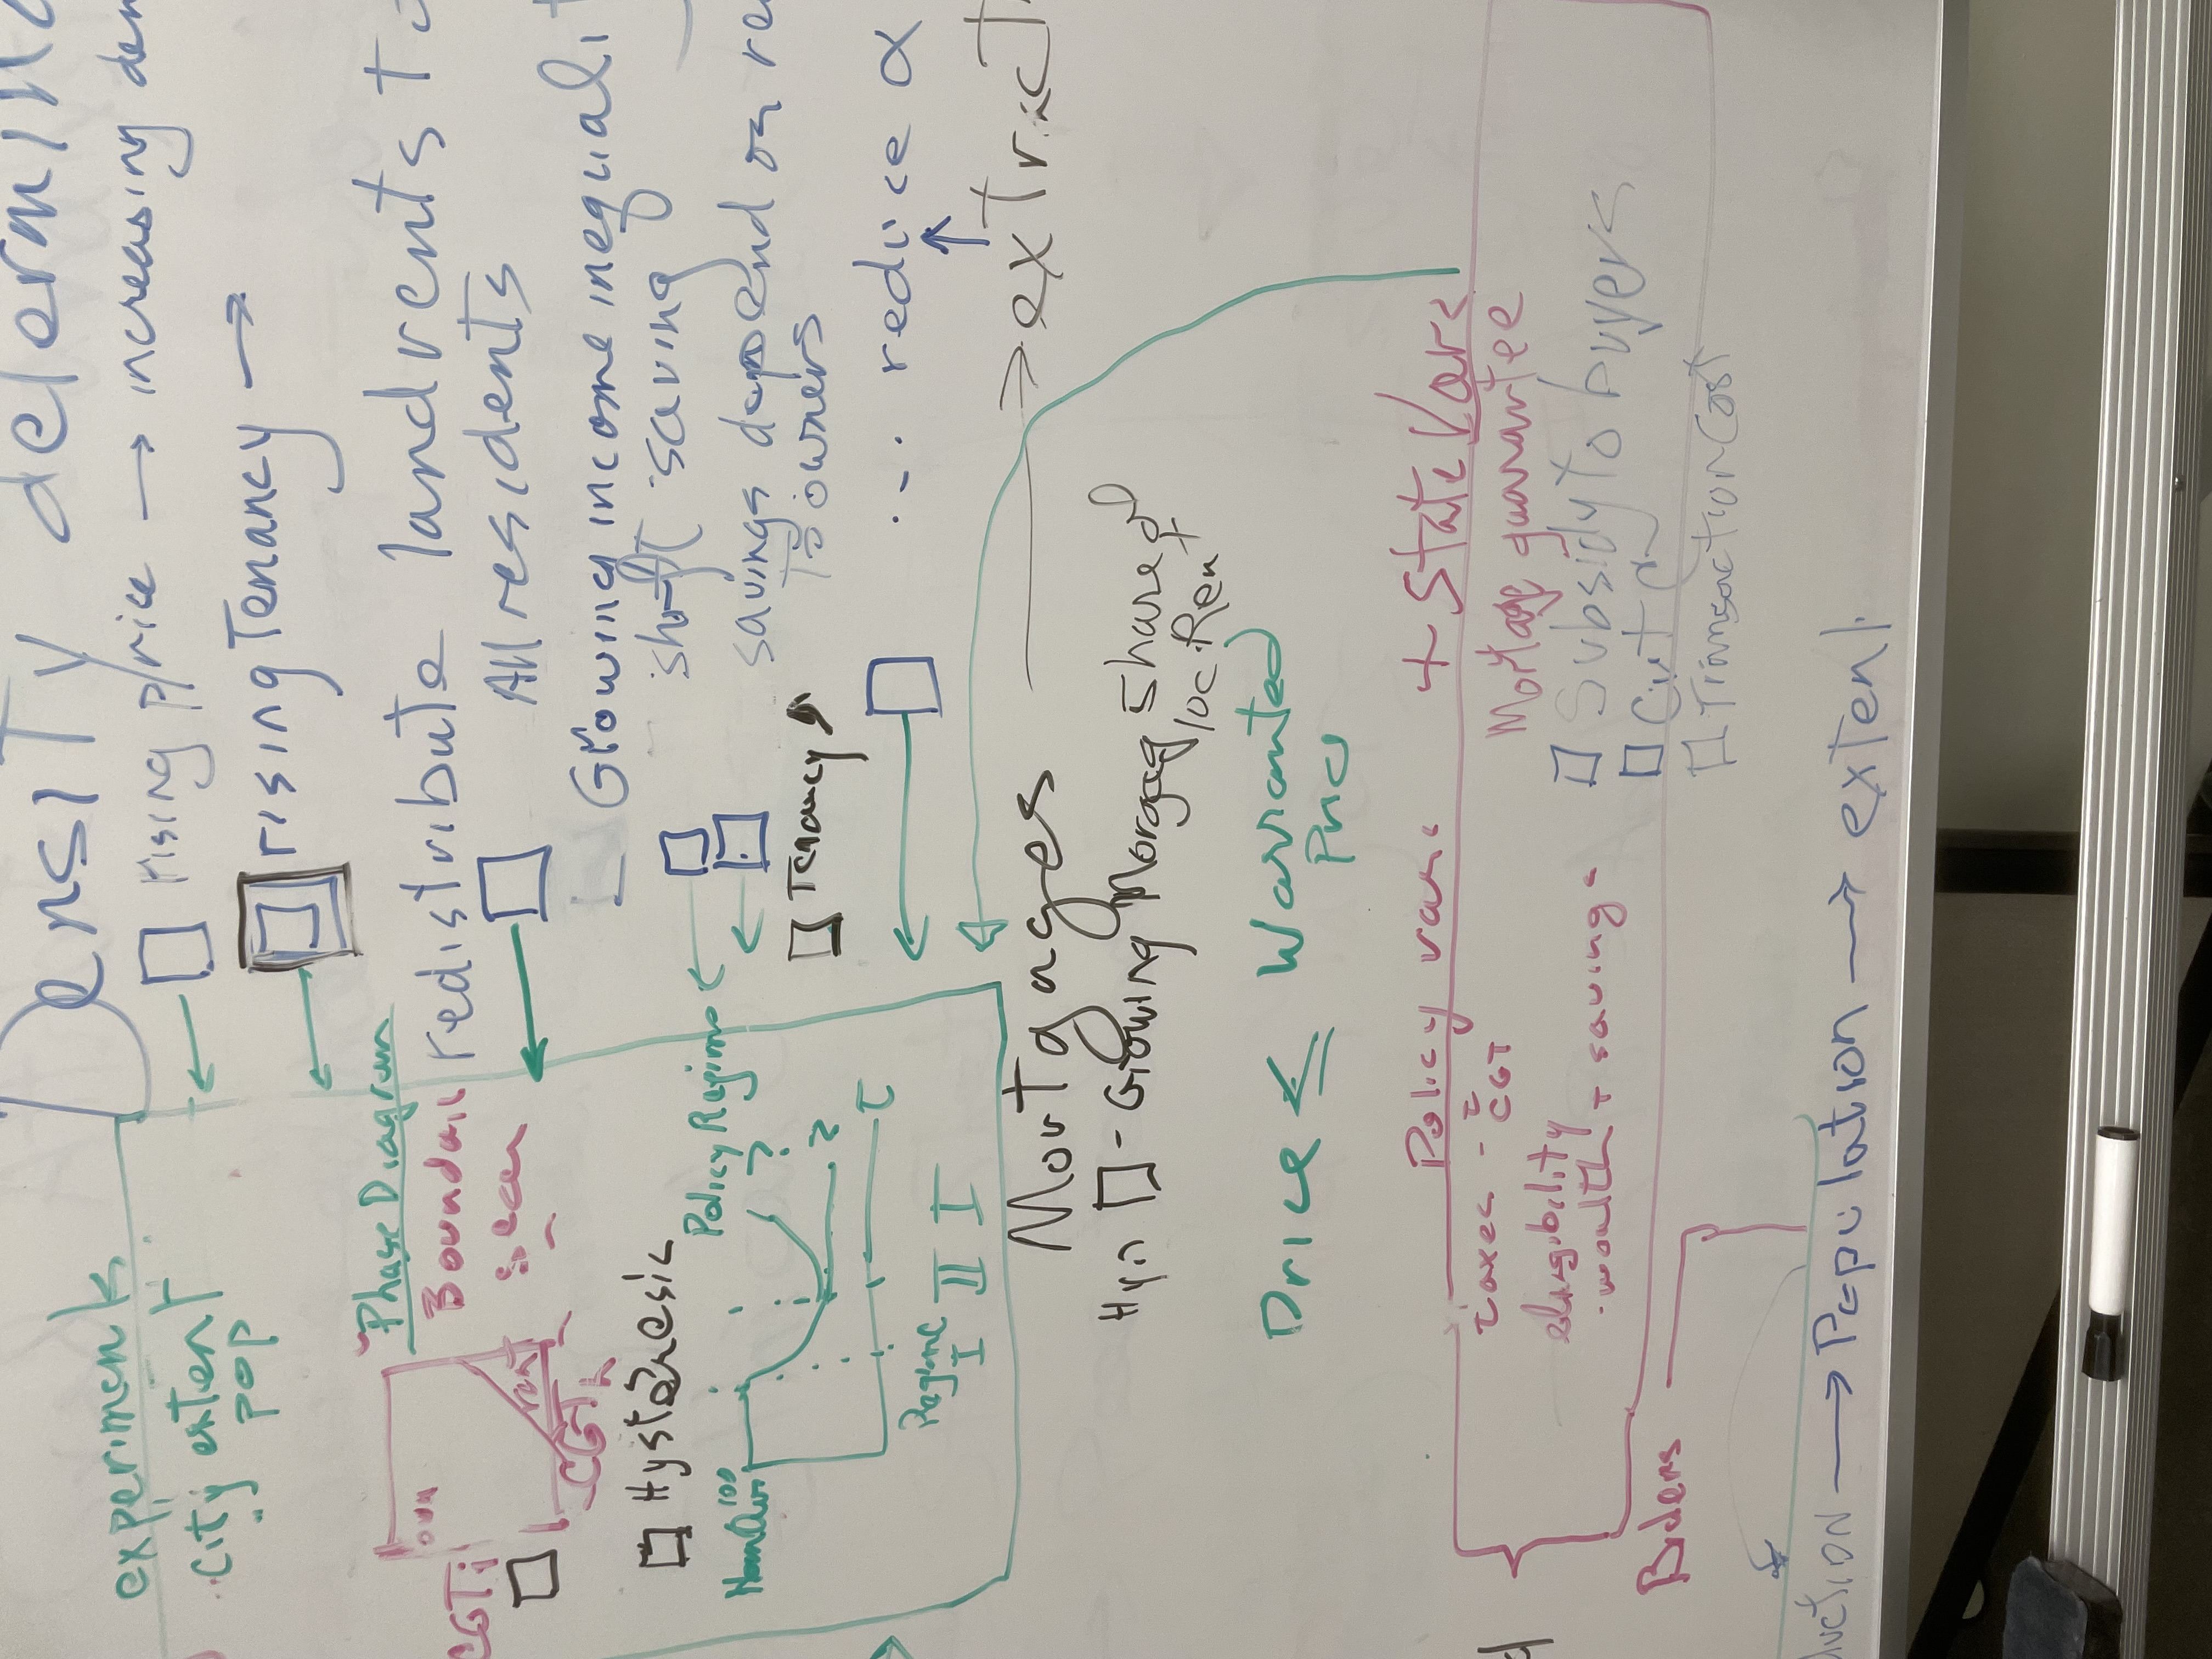
\includegraphics[scale=.5, angle=-90]{fig/IMG_2689.jpg} %Density determination

%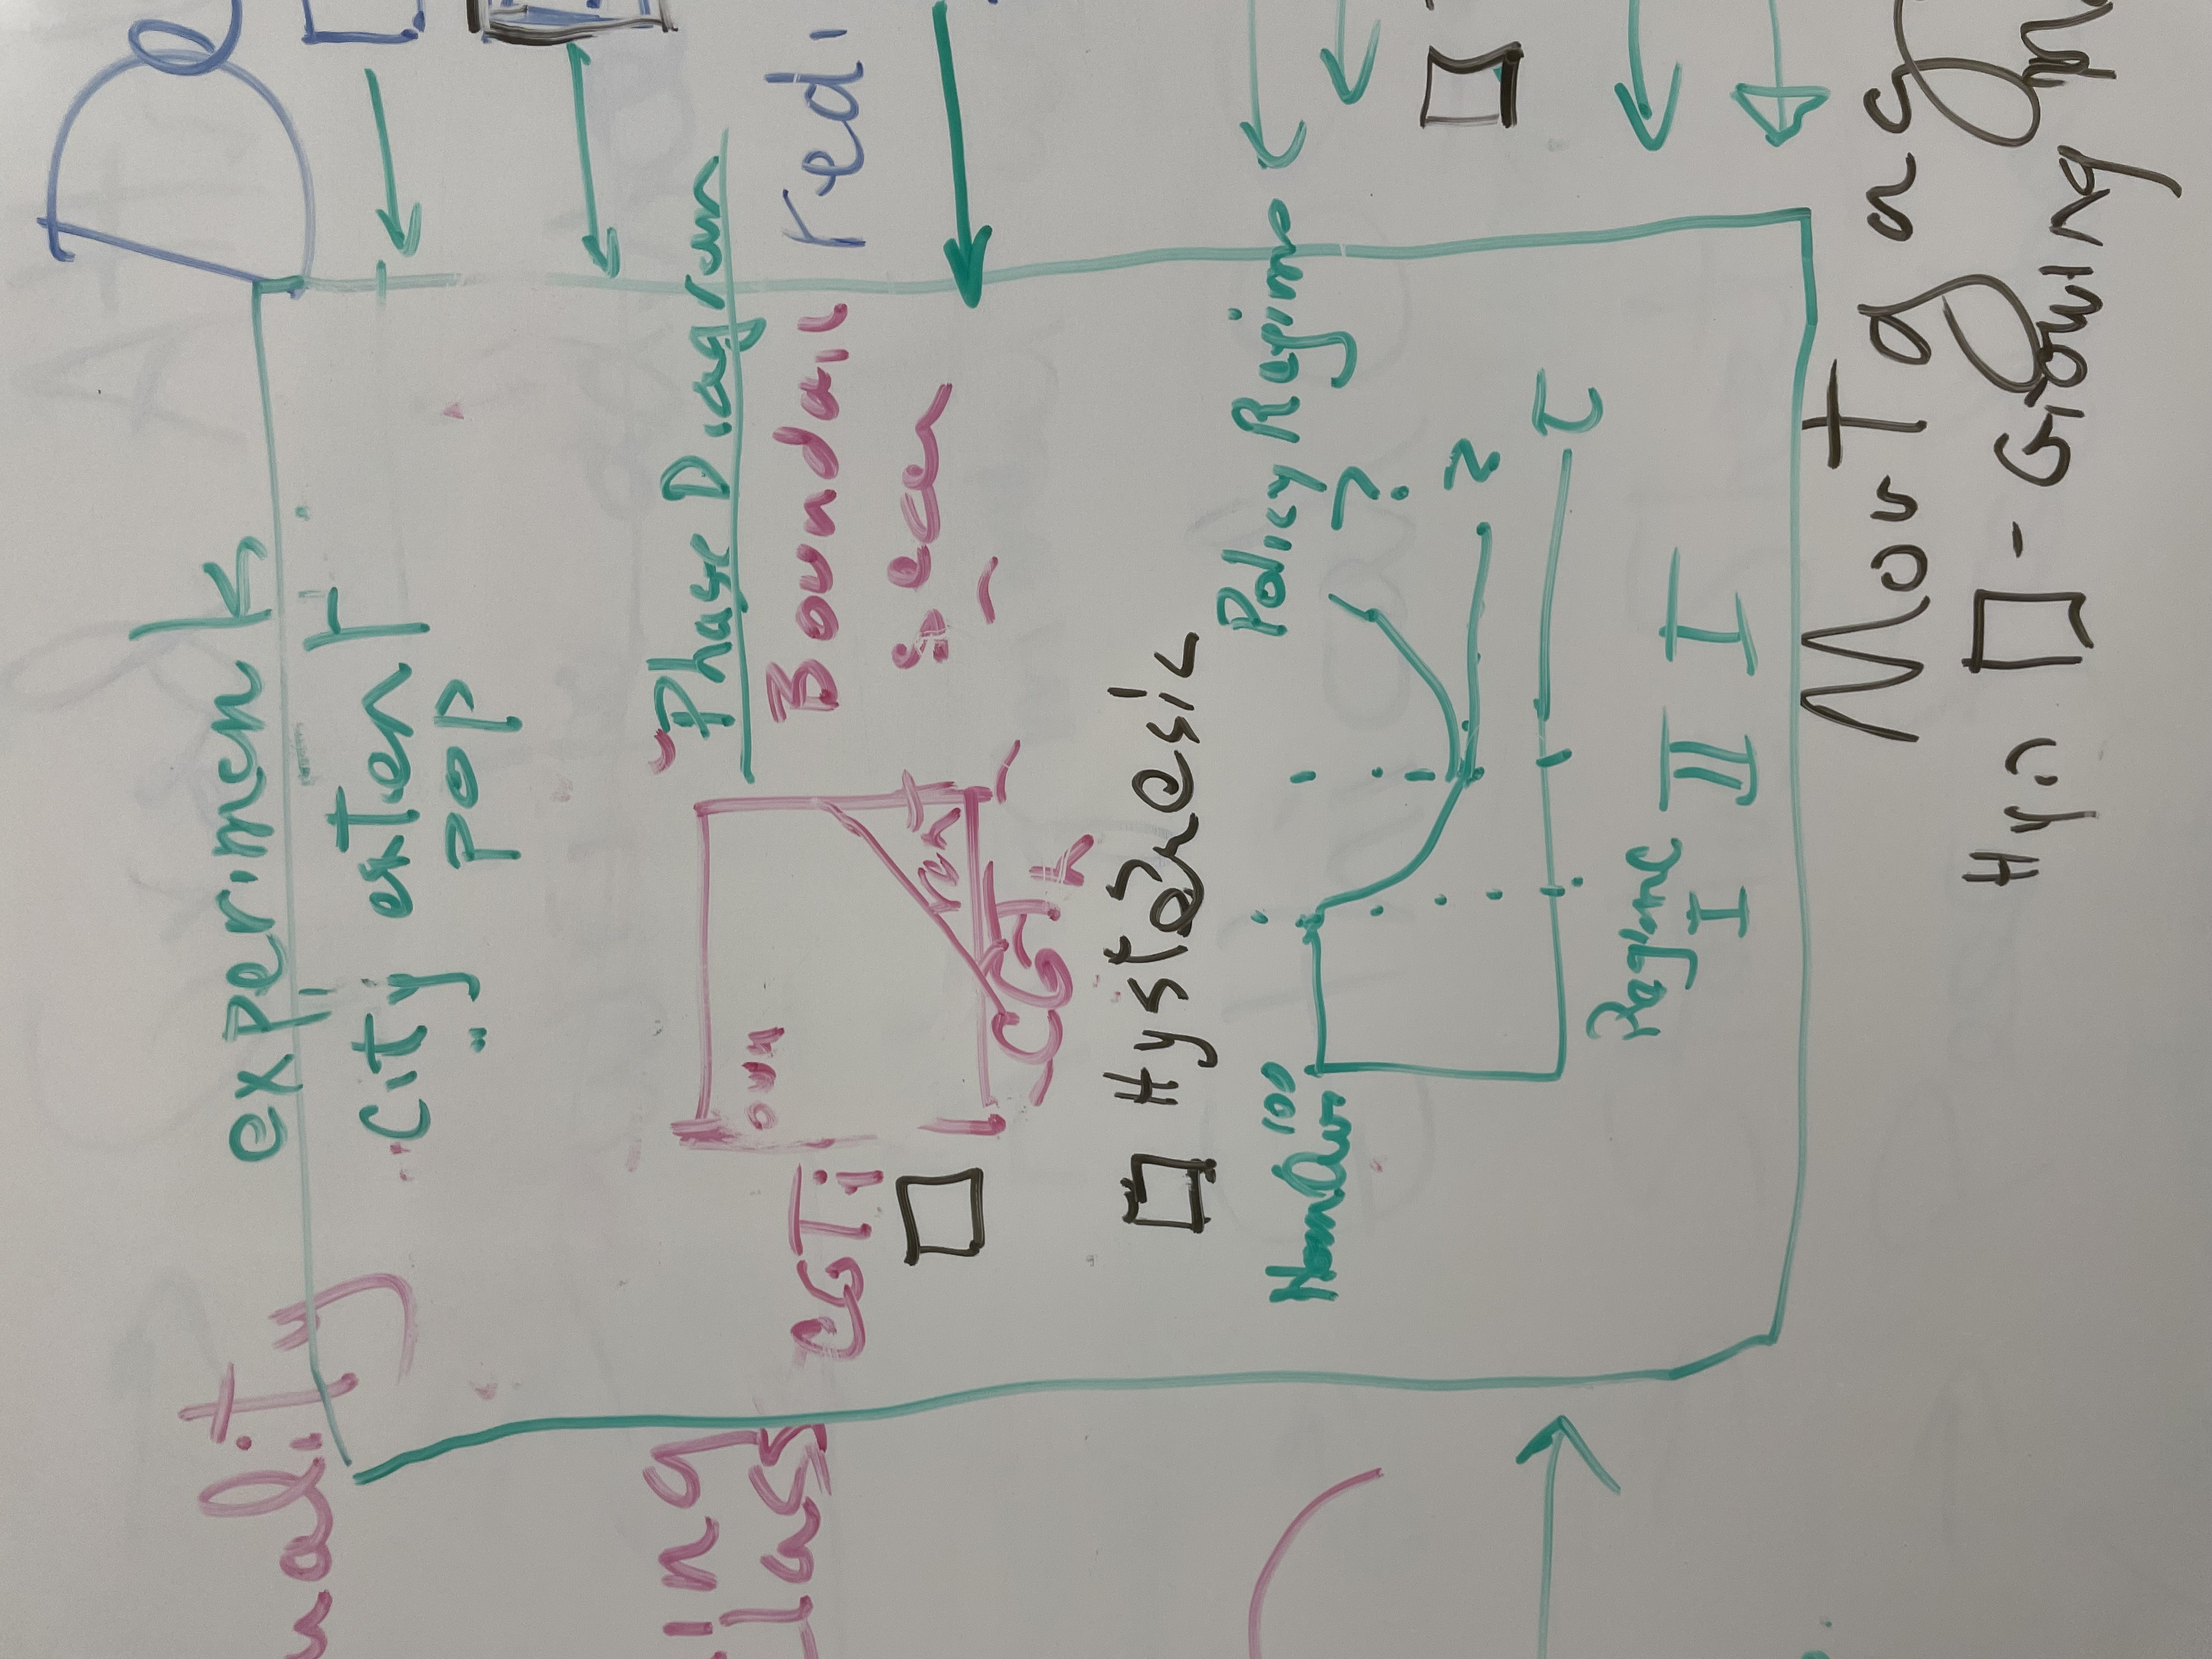
\includegraphics[scale=.5, angle=-90]{fig/IMG_2690.jpg}% 2 FIGURES NEEDED  
%$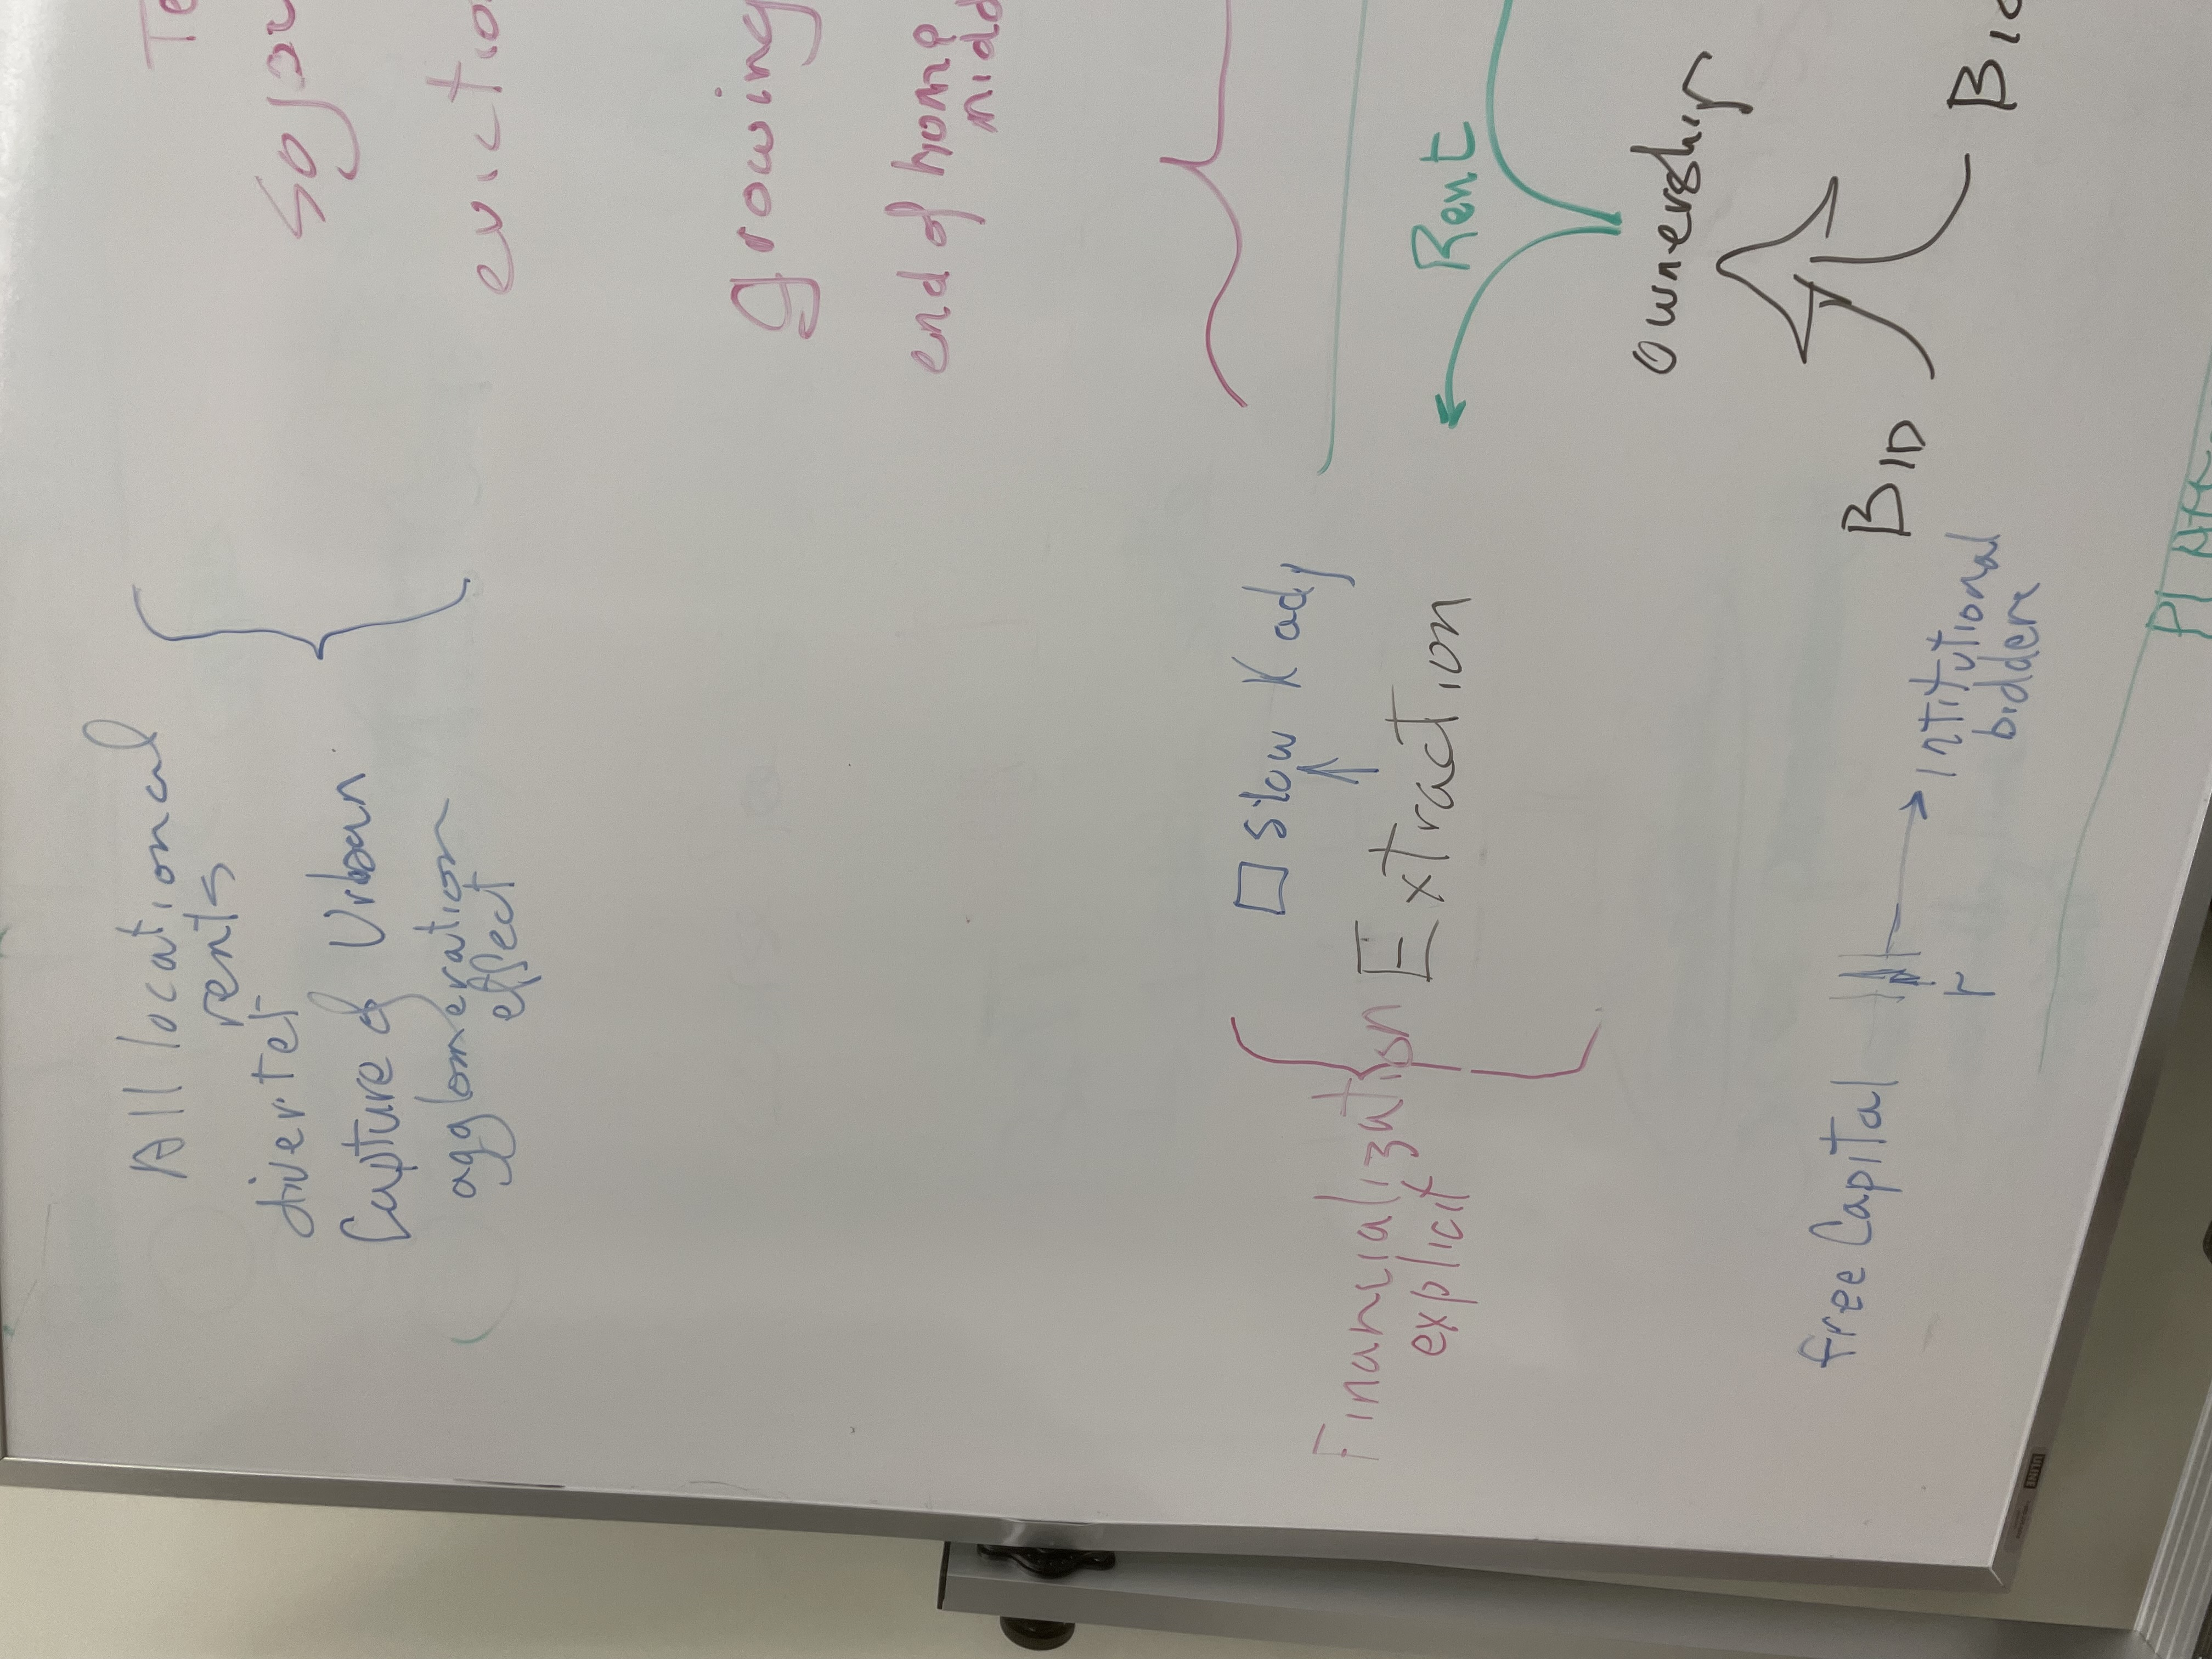
\includegraphics[scale=.5, angle=-90]{fig/IMG_2692.jpg}

To illustrate a decline in investment we can reduce Kadj.

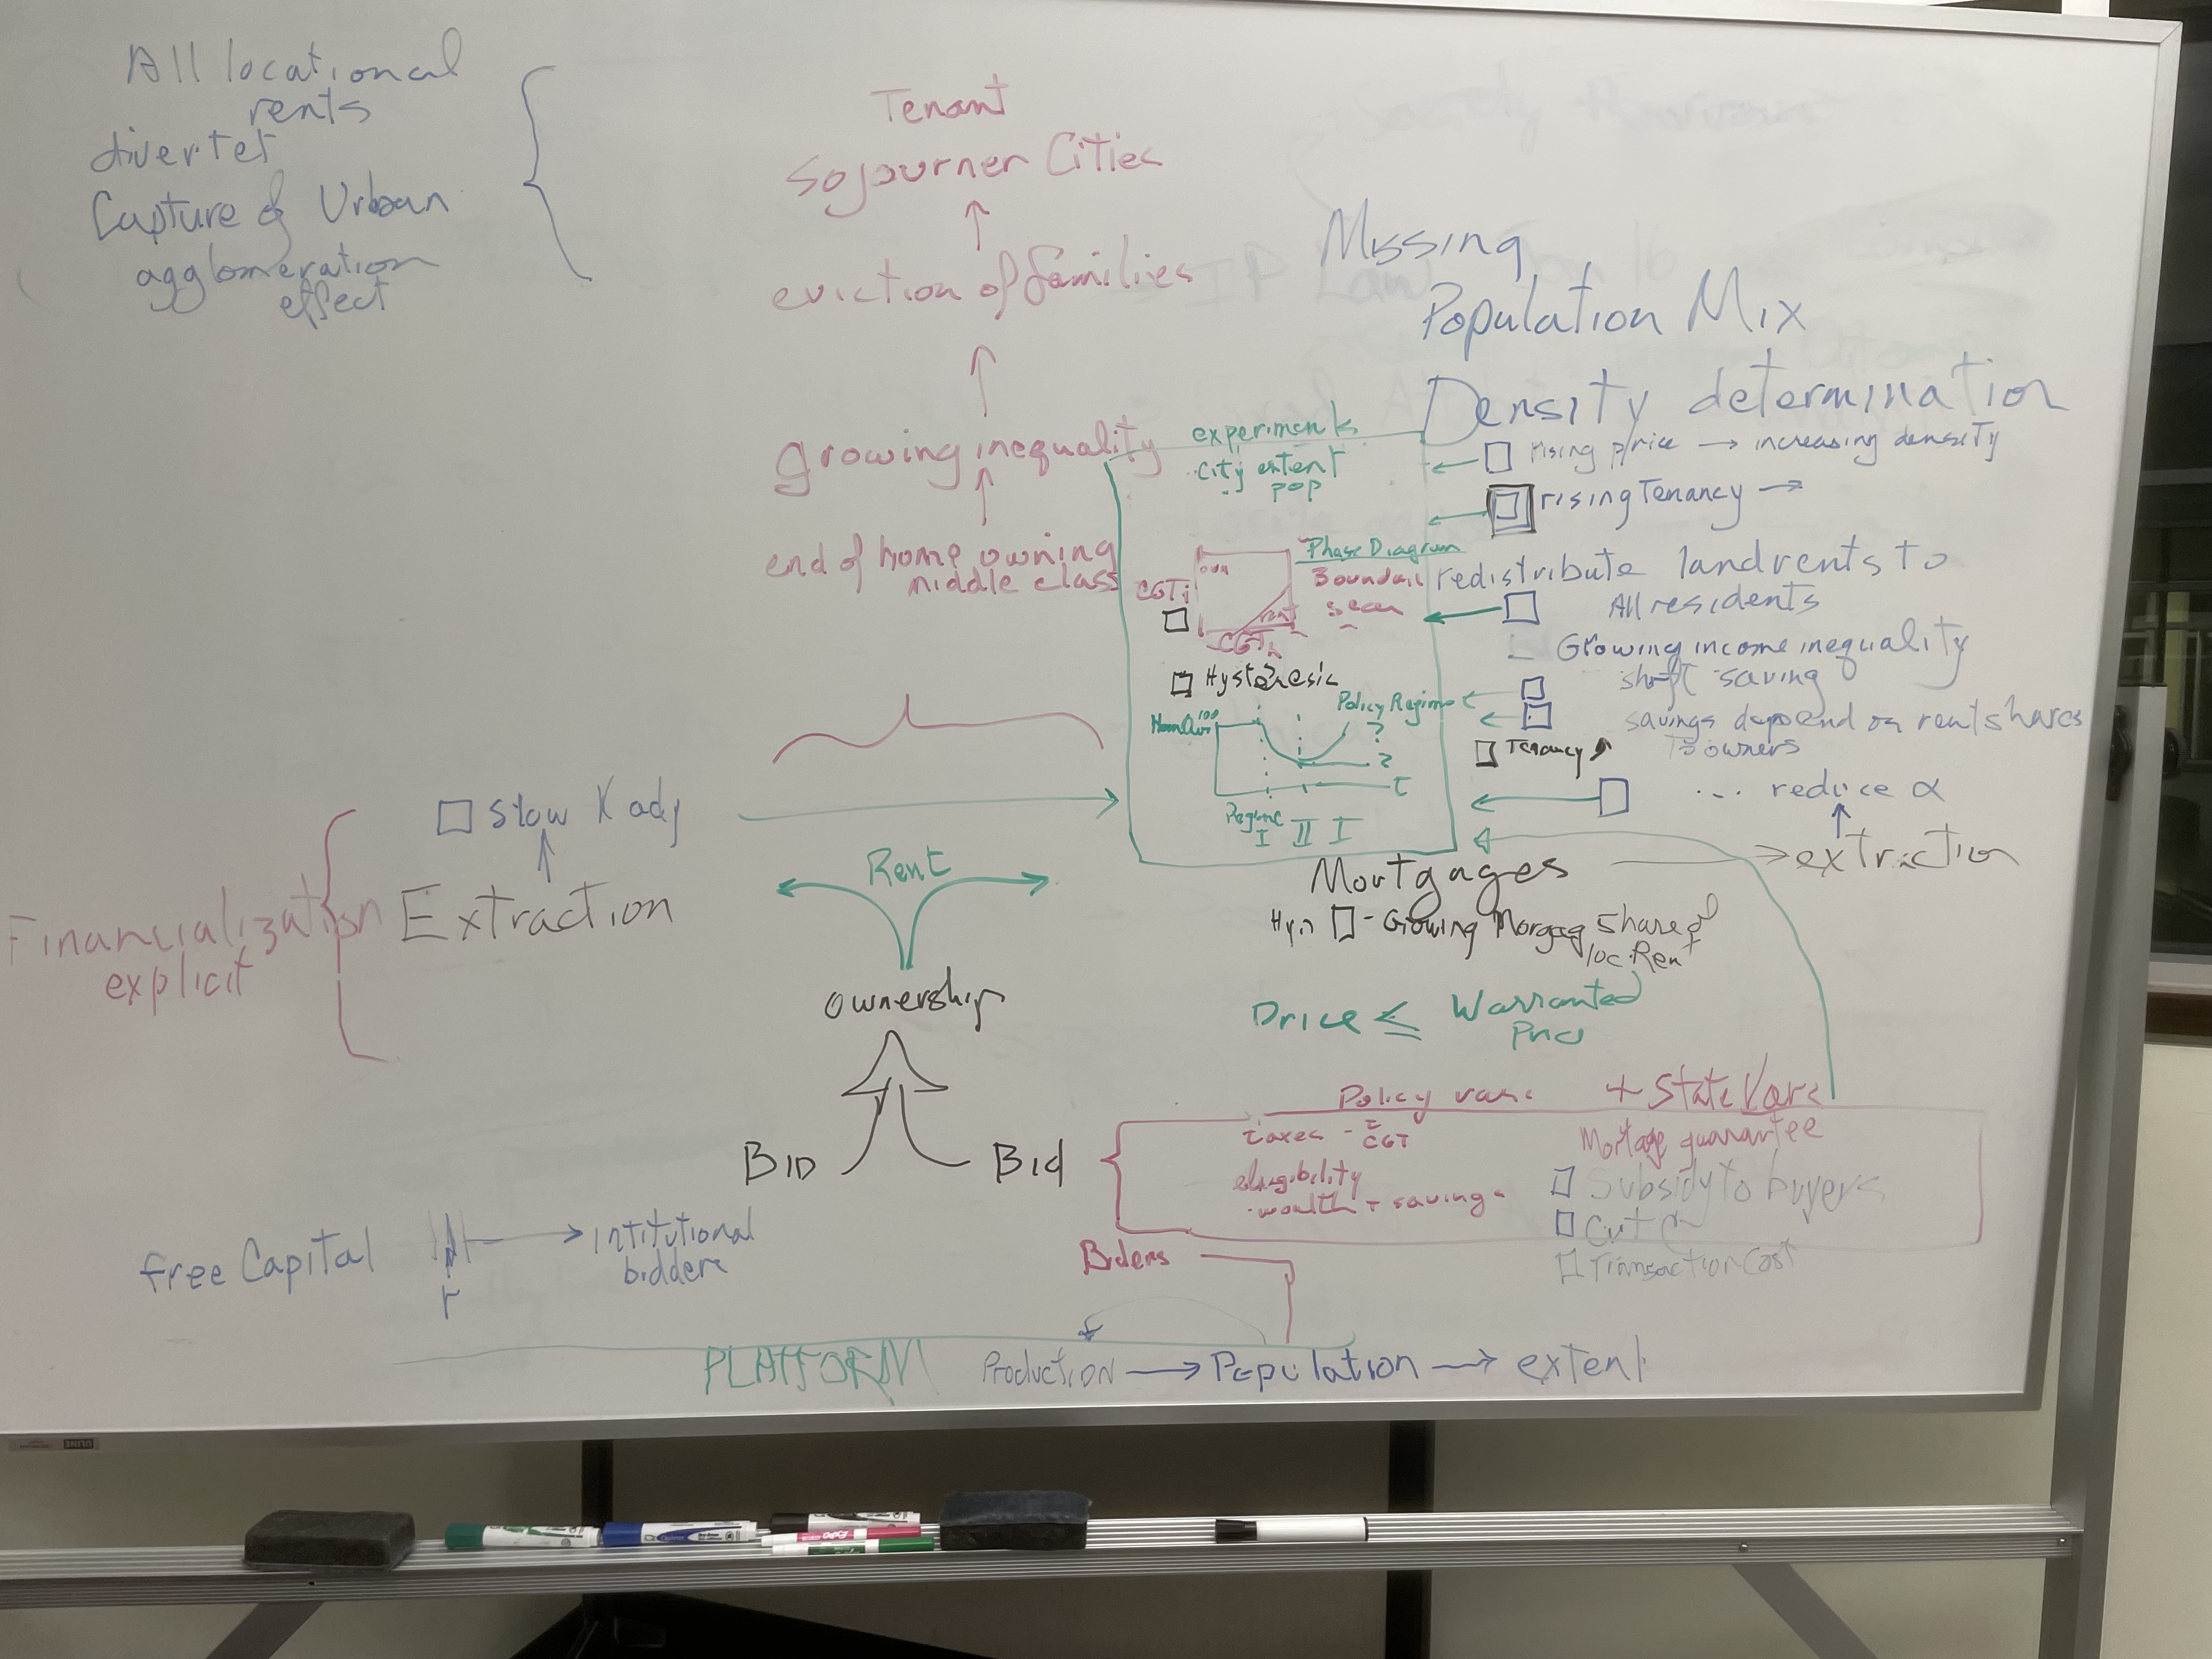
\includegraphics[scale=.5]{fig/IMG_2693.jpg}



Initially, 100\% of locational land rent accrues to residents. In the end, 100\% accrues to the owners of financial capital. Total rents at the end of the period of growth are eight times their initial size.\footnote{Recall that the radius of a circular city is proportional to the wage premium. Rent can be visualized as a cone of volume $\pi r^2 h$ where $h$ is the wage premium. If we double $h$, the volume is increased by a factor of 8.}



 \section{Implications for urban productivity}

 To explore the impact of financialization on productivity we introduce explicit links between ownership and .productivity          %%% NO

\part{Extensions} \label{part-extensions}
% \part{Analysis, Interventions, and Policy} \label{part-system}
\chapter{The Major Extensions}



\chapter{Old Analysis - Experiments and notes}
The two main hypotheses of this thesis are, 
\begin{enumerate}
 \item that the financial sector affects the ownership of housing and the class structure of society, 
    \item that this may have implications for urban productivity. 
\end{enumerate} 
Many parameters in the model will have some effect, but we have to focus on policy-relevant parameters. These a) can be manipulated, and b) can have measurable effects.


\section{Effect of the financial sector on ownership} 
We need to have 
\begin{enumerate}
    \item a set of measurements if ownership

        \begin{enumerate}
        \item number of homes, share of homes by category(owner occ, owner rented), 
        investor rented
        
\begin{tabular}{|r|c|c|c|}\hline
            & owner occ& owner-retired & bank-rented\\ \hline
number      & && \\ \hline
share       & && \\\hline
\end{tabular}

        \item Aggregate Mortgaged share of owner-occupied homes over time 
\[M_t=((1+r)**2-(1+r)**t) / ((1+r)**20-1)\]
\[Share\_mortgaged =\frac{\sum_i M_{,i}}{\sum_iP_{,i}}\]
        \item
        \item
        \end{enumerate} 


I imagine an output like this:

\begin{figure}
\centering
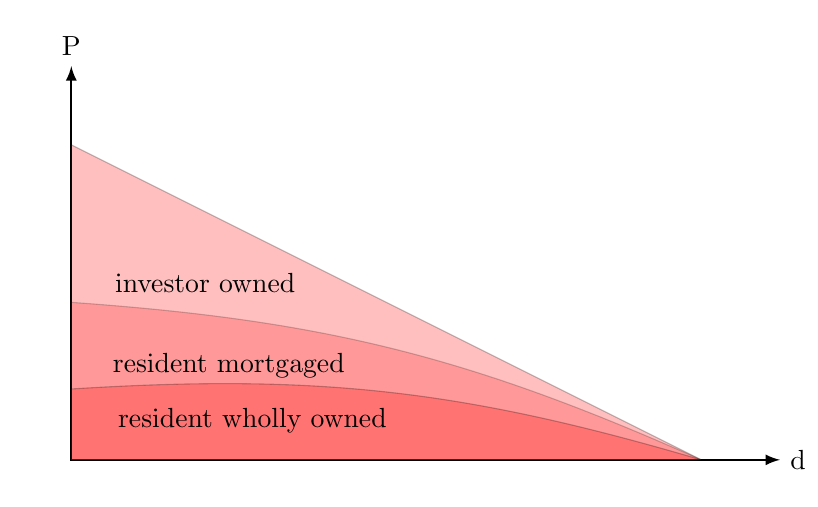
\begin{tikzpicture}
  \draw [thick, latex-latex](0,5)node[above]{P} --(0,0)--(9,0)node[right]{d}; 
  \draw[fill=red, opacity=.25](0,0)--(0,4)--(8,0);  
   \draw[fill=red, opacity=.2](0,0)--(0,2) to [bend left=10](8,0);  
   \draw[fill=red, opacity=.25](0,0)--(0,0.9) to [bend left=10](8,0);
   \node at (2.3,.5)[]{resident wholly owned};
   \node at (2,1.2)[]{resident mortgaged};
   \node at (1.7,2.25)[]{investor owned};
\end{tikzpicture}
\caption{GENERATE THIS FROM DATA}
\label{fig:enter-label}
\end{figure}


A similar picture with time on the horizontal axis

    \item parameters of the financial sector  that might affect that structure
    \begin{enumerate}
        \item capital gains tax
        \item interest and mortgage differentials
        \item tightening mortgage limits for owners
        \item transaction cost
        \item density
        
    \end{enumerate}

We can stabilize a city and then make a change to see the effect.

    
\end{enumerate}
\subsection{Results}
These are impressionistic notes from early batch runs.
\begin{itemize}
 \item increasing density range [100, 300, 400, 600]
    \begin{enumerate}
        \item ownership share peaks between 400 and 600. ***
        \item increases mpl
        \item increases firm size
        \item increases fir numbers
        \item decreases peak k
        \item increases city extent
    \end{enumerate}
    
    \item increasing subsistence wage range [30000, 50000, 70000, 90000]
    \begin{enumerate}
        \item decreases ownership share !??. 10 T->100\%  40-> 30\%
        \item seems to reduce mpl
        \item increases firmsize 
        \item Workforce diverges between 50 + and 70 dwn. ***
        \item decreases city extent
        \item increases then decreases firm capital ***
        \item slows growth of workforce

     \item increasing gamma range [0.1, 0.09, 0.08 ]
    \begin{enumerate}
        \item ownership share       
        \item mpl   up              
        \item firm size at up .09 dips and rises   
        \item total workforce up at .09 dips and rises
        \item number of firm number up at .09 dips and rises
        \item k    up peaks at .08                 
        \item city extent    up at .09 dips and rises          
    \end{enumerate}

     \item increasing discount rate.  range [0.1, 0.09, 0.08 ]
    \begin{enumerate}
        \item ownership share  strange sawtooth, generally rising
        \item mpl     no effect              
        \item firm size       no effect         
        \item number of firm number no effect 
        \item k           no effect           
        \item city extent    no effect           
    \end{enumerate}

    
    \item max\_mortgage\_share': [1.0, 0.9, 0.8, 0.7, 0.6]
    \begin{enumerate}
         \item ownership share  strange sawtooth, generally rising
        \item mpl     no effect              
        \item firm size       no effect         
        \item number of firm number no effect 
        \item k           no effect           
        \item city extent    no effect               
    \end{enumerate}


 \item increasing'ability\_to\_carry\_mortgage': [0.35, 0.28, 0.2]
   \begin{enumerate}
         \item ownership share  strange sawtooth, generally rising
        \item mpl     no effect              
        \item firm size       no effect         
        \item number of firm number no effect 
        \item k           no effect           
        \item city extent    no effect  
     \end{enumerate}


      \item increasing 'savings\_rate': [0.5, 0.3, 0.2]
   \begin{enumerate}
         \item ownership share  raises saw tooth
        \item mpl                   no effect
        \item firm size             no effect         
        \item number of firm number no effect 
        \item k                     no effect           
        \item city extent           no effect  
     \end{enumerate}

  
   \begin{enumerate}
         \item ownership share  
        \item mpl            
        \item firm size            
        \item number 
        \item k         
        \item city extent   
     \end{enumerate}
    \end{enumerate}
    


\section{Effect of the financial sector on productivity}
We need to have  
\begin{enumerate}
    \item a set of measurements if ownership
    \item parameters of the financial sector  that might affect that structure

\end{enumerate}

  
\section{Experiments}
  \begin{enumerate}
    \item effect of reducing transport cost $c$
    \item effect of adding a service sector $N_{total} = N(1+z)$ then $N^\gamma \rightarrow  N_{total}^\gamma$
    \item \textbf{effect of adding a service sector whose size depends on the retained income of residents.}
    \item changing density
    \item low-wage immigrants
    \item effect of interest rate spread on housing ownership
    \item 
    \item 
    \item 
    \item 
    \item 
   
    
\end{enumerate} 
    
\end{itemize}
\subsection{What else will affect price and should be included in the regression?}

\newcounter{foo}
\newcommand{\num}{\addtocounter{foo}{1}\thefoo. &}
\newcommand{\Rnum}{\addtocounter{foo}{1}\thefoo. &\vspace{-.3cm}\color{red} }
\section{Variables to track}

\begin{tabular}{lp{8cm}l}
\hline
\num Wage premium  &$\omega$\\
\num workers in a firm &$n$\\
\num workers in a firm &$n$\\
\num output of firm &$y_F=y$\\
\num Firm MPL& $\beta y_F/n$ \\ 
\num  population of workers &$N=F*n$\\
\num total population & $factor * N$\\

\hline
\num number of homeowners &\\
\num number of tenants &\\
\num number of institutional owners &\\
\num number of homeowners who rent&\\
\num number of homeowners with second home&\\


\hline
\num total taxes & $\sum_j t*P_j$ ?\\
\num taxes invested in productivity& $tProdShare * total_taxes$\\
\num taxes invested in Amenities& $tAmenShare * total_taxes$\\

\hline
\Rnum  urban firm-generated surplus &  $(A * N**beta) - (N/n_R * Y_F)$ \\
\num \\

\num total homeowner wealth& $\sum_i(P_I - M_i) + \sum_i S_i$\\
\num homeowner savings invested in productivity & $SProdShare * \sum_i S_i$\\
\num total city output& $Y=F*y$\\
\num  Total Factor Productivity (TFP)& $\frac{Y}{rk+(\omega+psi)N}$\\
\num external investment & $\sum_f K_F$\\
\hline
\end{tabular}

\begin{tabular}{lp{8cm}l}
     &  \\
     &   \\
\num expected rate of price increase over T& $\dot P^e_\mathbb{T} = \left(\frac{\frac{1}{r}\die{\omega}{t} }{P_T}\right)^T $ \\
\num total rent on property& $N(\omega +\mathbb{A}^{net})$ \\
\num total urban locational rent& $\pi(\omega +\mathbb{A}^{net})^2/3c$ \\
\num dissipated rent &$\sum_i^N c_id_i$ \\ 
\num available rent. & $\sum_i^N(\omega -cd +\mathbb{A}^{net})$\\
\num Mortgage interest captured by the finance sector& $MortI=\sum_i r_iM_i^{balance}$ \\
\num Total rent captured by the finance sector& $FinRent = MortI + \sum_j R_{N, j}$)\\
\num share of city-owned by finance& $\sum_i^N M_{i,t} +$ value of property ???\\

\num locational surplus   &  $Surp = \sum_j (/omega- c*d) $\\
\num financial share of surplus & $FinSurpShare = FinRent / Surp$\\
%\num  Amenity & $\mathbb{A}^{net}$\\ 
    %fixed. We want total amenity including utility
\num financial share of city & $FinCityShare = \sum_i^N M_{i,t}$ \\
   %two parts  separately -- (pop with density and seed) * omega
\num GDP Growth &$N(\omega +\mathbb{A}^{net}) + r F(k^U-k^R)$.\\
            &(not a rate) ($(k^U-K^R)=\Delta k$)\\
  \end{tabular} 

 Additional items 
\begin{enumerate}  
\item Total Rent captured by the finance sector is the sum of the interest collected on all mortgages ($\sum_i r_iM_i^{balance}$), where $j$ indexes households,) plus the \textbf{net} rent on rented housing ($+ \sum_j R_{N, j}$), where $j$ indexes properties (Just those owned by the bank Those not owned by the bank represent extractions by small landlords. The Financialization study had a name for this class.).

\item Rent captured by the finance sector divided by urban surplus is the share of surplus captured by the financial sector






\item Output of a  typical rural firm, Equation~\ref{eqn_Rural_output} 
\[Y_R=\frac{n_R*\psi}{\beta_F}\]

The output of a rural firm is a constant  providing a reference line for the output of the urban firms. %calculated in appendix 2 to get initial values

  \item excess profit: all profit is excess because the cost of capital has been covered.
    \[\Pi^{excess}=F*(y_{U,t} - r*k -)(\omega+\psi)n_{U, t}\]

 \[RB = M_0 * (((1 + r)^20) – ((1 + r)^p)) / (((1 + r)^n) – 1)\]

Where:

    P = principal amount of the loan (\$10,000 in this case)
    
    r = monthly interest rate (r=r\_prime + margin)
    
    n = total number of payments 20 years, one per year
    
    p = number of payments made so far (12 in this case)   

\end{enumerate}



 \subsection{for the price model}
% make sure the regression model makes sense. price should fall with distance by the present value of the cost of transportation: $cd/r$. Only $d$ varies across properties. In a regression for price the beta for distance should be $c/r$. This can serve as a check  

% We can think of properties at the same distance as a "transportation-equivalent neighbourhood'' such that 
% \[d_j=d_k,\]
% where $d$ is distance.  (or $\omega-cd_j=\omega-cd_k$.  We expect prices to behave the same in these neighbourhoods. You can add dummies for other neighbourhoods to the model later if you add neighbourhood features or specific amenities. 

% In the regression you just add $d_j$

\subsection{Estimation P-dot from the model }
% The higher the rate of price increase the more people will want to buy or hold the property. 

% In the regression you just  $\dot P_{t,j}$

% By definition, $\dot P_{t,j}$ is \[\dot P_{t,j} =\frac{P_{t,j}-P_{t-1,j}}{P_{t-1,j}}\] for each property. This can be calculated property by property. What if there are very few properties that have changed hands  in the last two periods? 


% Will it serve as as plausible value for $\dot P_{t,j}$? Yes.

% The average of this value across the neighbourhood is the average neighbourhood price growth. It WILL vary by distance. To see this consider a rise in $\omega$ and two properties, one at the centre and at the edge of the city. The one at the centre has a price $(\omega + a\psi)/r$ and the edge property  has a price $(a\psi)/r$ Both increase in value by $\Delta\omega/r$, so the rate of price growth must differ.



\subsection{r-code to graph remaining}
The figure below illustrates the path of Mortgage remaining, which we need for certain wealth calculations (if an owner wants to get a second mortgage.
)
% n<-240]%
% r<-.05/12
% t<-seq(0,240,1)
% rm<- ((1+r)^n-(1+r)^t) / ((1+r)^n-1)
% plot( rm) 
In Python 

\[M_t=((1+r)**2-(1+r)**t) / ((1+r)**20-1)\]

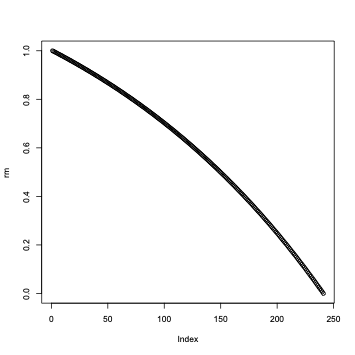
\includegraphics[scale=.25]{fig/declining-balance.png}
  
    


\section{Main}

% Get banks 'We are the biggest innovators in history quote'
%``Financial engineering has created a rentier class, a modern feudal system, and the biggest beneficiaries of all that extra debt have been the bankers.'' Times, Sunday Times (2016) 


% Repeat from introduction contributions
% Note multiple drivers - 
NOTE \textbf{not sensitive to any advantage being true all of the time. etc } IN THE STRUCTURE.
% can be thought of as regimes containing tipping points, the feduciary duty of governance is to sustain the regimes society chooses, to make that process of choosing tractibel labs, Kahane.

% MAIN PLOTS DIRECT ANALYSIS
% RESILIENCE ANALYSIS 
% DISCUSSION AND EXTENSIONS

In the base model, we only allow the radius of the city to change, and not the density and firm hiring behaviour.\footnote{Complex city form, density patterns, and alternative hiring patterns, can be easily incorporated in the computation model. We expect that they would not significantly affect our conclusions.}  
% model rules, and individual 
%and the job search process. 
% In practice, many other factors impinge on these choices. %additional decision factors, agents, driving variable, and \gls{stochastic} elements enter the model. 



\section{Financialization: implications of  population or productivity growth}

Our model is a dynamic  one, concerned with growth and financialization. We have described the components separately and  generally described them in static terms. Rent theory in  particular was a static described as though rents never changed. With a small addition to the figure from Chapter~\ref{chapter-space}, however, we can begin to explore the effects of rising population or productivity. 

In Chapter~\ref{chapter-space} we limited our discussion to what is termed differential land rent, which results from differing transportation costs. It is the key concept in the Alonzo model. The city grows until adding more land at the edge of the city generates no land rent because the value of access to the city centre is eaten up by transportation costs. If the population or productivity increases   drive up the the value of access, the price of land  will rise across the entire city. The higher land value would eventually lead to an expansion of the housing stock, moving the city edge in Figure~\ref{fig:absoluite_rent} outward. The differential rent would expand as well.

If we focus on the increase in rent before the housing stock can expand, which we show as the orange rectangle in Figure~\ref{fig:absoluite_rent}, it is clear that increased productivity is translated into increased rent on existing properties.\footnote{The orange rectangle corresponds in this setting to what Marx called ``absolute rent'' \cite{dasilvaAbsoluteRent2018}. } The orange rectangle represents value of the increase in the wage across the entire city. When the stream of rent it is discounted to the present it represents \textbf{the total increase in land value across the entire city}. 

Like Marshall's quasi-rent, This rise in rent provides an incentive to expand the stock of productive housing capital.  It does not disappear  as a quasi-rent would, however. Instead it appears as a windfall gain for owners. In our analysis it has another effect: it will attract speculative purchases of the existing housing stock. It is one of the drivers of the financialization of the housing stock. 


\begin{figure}
    \centering
    
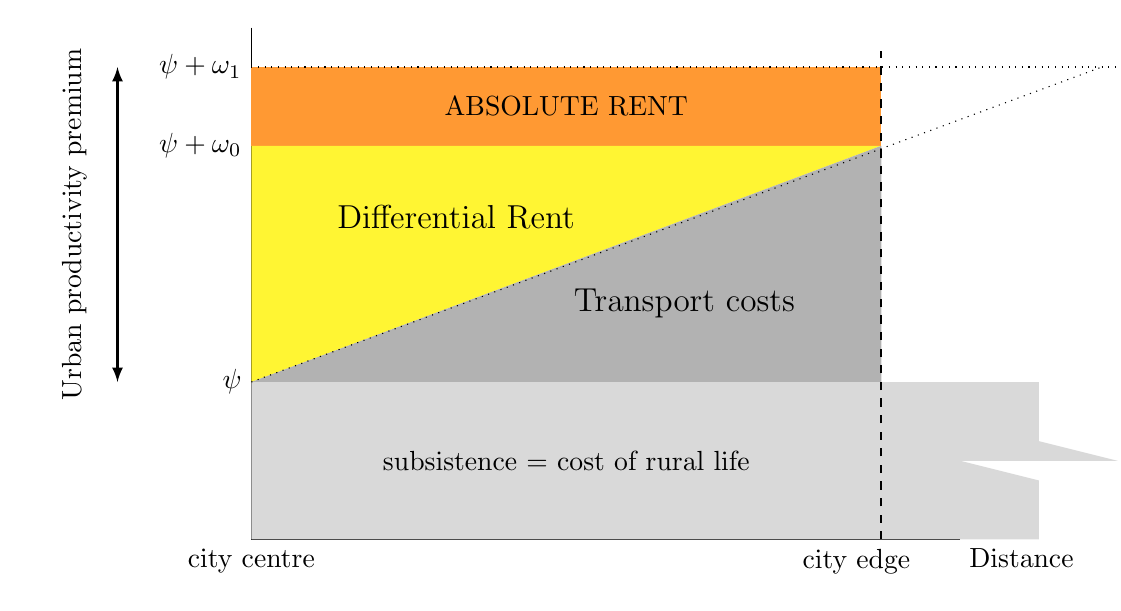
\begin{tikzpicture}[domain=0:2]
%\draw[thick,color=gray,step=.5cm, dashed] (-0.5,-.5) grid (12,5);

\draw[line width=.01 ] (1,6.5) -- (1,0)node  [below] {city centre}--(10,0) node[below right] {Distance};
%\draw[line width=.01, green ] (0,0) -- (10,0) node[right ] {Distance};
\node[below,text width=2cm]at (9,0) {city edge};

\fill [orange!80]  (1,5) --(1,6)--(9,6) --(9,5)--cycle;
\fill [yellow!80]  	(1,2) --(9,5)--(1,5) --cycle;
\fill [gray!60] 	(9,5) --(1,2)--(9,2) --cycle;
\fill [gray!30] 	(1,0) --(1,2)--(11,2) --(11,1.25)-- (12,1)-- (10,1)--(11,.75)--(11,0)--cycle;



\node	at 	(1,5)[left]{$\psi +\omega_0$} ;
\node	at 	(1,6)[left]{$\psi +\omega_1$} ;
\node	at 	(1,2)[left]{$\psi$} ;

\draw[thick , dashed] (9,0)  -- (9,6.2); 
\draw[dotted] (1,6)  -- (12,6); 
\draw[dotted] (1,2)  -- (11.8,6); 

%\draw[thick,color=red] (1.5,0) -- (1.5,1) node[below right] {Fixed cost} -- (1.5,1.5) --(10,3.25)node[above left] {total cost};

\node at (5,5.5)[] 	{ABSOLUTE RENT} ;
\node  at (6.5,3)	{\large Transport costs};
\node  at (3.6,4.1)	{\large  Differential Rent};
\node at (5,1)[] {subsistence = cost of rural life} ;
\node at (-1.25,4)[rotate=90] {Urban productivity premium} ;
\draw[thick,latex-latex] (-.7,2) -- (-.7,6) ;
\end{tikzpicture} 

    \caption{Growing productivity, population, and rent. Rising productivity and/or population will increase rents. With slow or no increase in density or area,  absolute rent grows and becomes a target for financial capital.  }
    \label{fig:absoluite_rent}
\end{figure}

\subsection {Productivity growth}
In this case, the orange rectangle in Figure~\ref{fig:absoluite_rent} shows the effect of an increase in the wage premium from $\omega_0$ to $\omega_1$. We can assume that the wage has been raised by firms in order to attract more workers because productivity has risen. An increase of this sort in our model may hae resulted  from past population growth generating additional agglomeration effects. Since such effects accumulate slowly, the figure illustrates an increase due to previous population growth that gradually brought improved methods and machinery, new products or even new markets. The    
The housing stock has not yet adjusted.  Any fraction of the increase in productivity  flowing into profits does not appear in the figure. 


Initially the increase in the wage would appear as increased saving and consumption for resident workers. For tenants, the improvement would be temporary. Landlords would realize that tenants could pay higher rent or new tenants would bid more for housing. The result is that non-resident owners would eventually extract part of  the increase in productivity. That fraction would grow as the financialization of the housing stock proceeded expanded 

In time the city would expand to provide new housing. The expansion would proceed until the diagonal line extended to the height $\phi+\omega_1$.\footnote{The figure only allows for increasing area and not increasing density.}  

Of interest here is that, at the moment represented by the figure, a significant rise in land rent across the entire city is in the future and therefore increasing house prices are predictable. Agents that foresee the capital gain would invest. The pool of new workers who can afford to purchase might be small, however, while the pool of available financial capital would be large. It is reasonable to expect that the increase in urban productivity would tend to drive increased financialization of the housing market.

In this situation there is a possibility that real estate investment might squeeze out productive investment. Finance would flow to expanding the housing stock, which is productive investment.  Would financial capital flow into investment in city firms or into speculative investment in existing housing? Real estate investment might  draw capital away from productive investment. A great deal might depend on assessments of the riskiness of the different investment channels.

\subsection{Population growth}
Population growth will operate on the same variables  but in a different way. There is a debate about whether urbanization drives  growth or growth drives urbanization. We observe in-migration as one apparently independent driver of urban population growth,  so it makes sense to examine the effect of an externally driven increase in urban population. 

Increased competition for housing will drive up rents and prices. The increase in rents will not affect owner-occupiers directly, although they might see and increase in boomerang children or an increase in opportunities to rent out part of a home. Both of these effects would tend to increase home values for owners, make them less likely put a home on the market. 

The increase in rents will affect tenants and in-migrants. It may eat into their consumption or savings. It will also drive some low-pay workers out of the city and increase wage demands. Wages will have to rise, probably reducing profit and investment in the city. The rising rents will have the tendency to increase financialization of the housing stock as in the previous subsection.

\section{Financialization: implications of the bidding rule}

There are some implications of the financialization mechanism:
\begin{enumerate}
\item A large $m$ magnifies the return. (The downpayment is smaller as a fraction of the price, increasing the investor's leverage). 
Given the  common rule that mortgage payments cannot exceed some fraction of disposable income, the wealthy will be able to borrow larger amounts and at lower interest rates than the less wealthy. At any distance from the centre they will be able to make a higher bid.

\item A lower mortgage interest rate increases the return by lowering interest payments. The cost of capital is known to differ for rich and poor.  The wealthy can generally borrow  at lower interest rates than the less wealthy. 

\item A lower discount rate $\delta$ reduces the subjective rate of return.  Poverty in assets and cash liquidity constraints are correlated with higher rates of time preference  \cite{carvalhoPovertyTimePreference2010}\cite{holdenPovertyMarketImperfections1998}. If agents discount at their borrowing rate, wealthier agents may have a lower subjective rate of time preference and therefore value properties more highly. 

\item Higher expected price appreciation increases the attractiveness of an investment. Financial corporations and the wealthy are likely to have better price forecasts than  the occasional home buyer.

\item Higher rents make the unit more profitable. Higher expected  rents may result from expecting greater price appreciation  leading to raising rents for tenants. Lower discount rates may give future rent increases greater present value.

\item Lower maintenance costs increase profits. There may be scale economies in the maintenance  of rented housing. 

\item Lower tax rates decrease holding costs and increase the value of the investment. There may be opportunities to shelter income with land held for investment (speculative) purposes. Tax treatment of income and capital gains as well as interest deductibility may also provide advantages for institutional buyers and investors.%\footnote{Case and Schiller \cite{LOST_CaseandSchiller} observe that (source?) `` \dots increases in real per capita income all are positively related to excess returns or price changes over the subsequent year.''} 
\end{enumerate}

Some  of these conditions (1-3) hold generally for wealthier actors. Others (4-7) may be available only to institutional investors.  Financial corporations in particular may have advantages relative to individual investors, making it reasonable to expect that financial corporations increasingly dominate urban land 
markets.\footnote{Fr\'ed\'erick Demers \cite{demersModellingForecastingHousing2005} found that the response of housing investment to interest rates has become more pronounced over time. This suggests a rising share of financial investors relative to buyers focused on housing services. Case and Schiller \cite{caseThereBubbleHousing2003} observe that `` \dots increases in real per capita income all are positively related to excess returns or price changes over the subsequent year.''}  

Since interest rates are lower for those with higher wealth, the analysis implies, consistent with the empirical evidence, that net returns for investment are increasing with wealth. Large wealth holders will get higher expected and actual rates of return on land than those with lower wealth holdings. Managers of large pools of capital will have an even greater   advantage. Overall, Equation~\ref{eqn-bid-price} implies  sales generally go to the richest participant.
 
%  \footnote{Case and Schiller \cite{LOST_CaseandSchiller} observe that (source?) 
%  `` \dots increases in real per capita income all are positively related to excess returns or price changes over the subsequent year.''} 

% The conclusion that we draw from the analysis above is that  financialization of urban housing benefits a rentier class of urban landholders. There is evidence that it benefits a globally distributed class of rentiers.  



\section{Financialization as system change} \label{section-system}
We established that, at least in theory,  financial institutions and the wealthy are likely to own increasing shares of the housing stock. the theoretical conclusions is consistent with what has already happened in the Canadian Housing market. Recent data from Statistics Canada \cite{fontaineResidentialRealEstate2023} suggests people who own more than one property in Ontario make up more than 25\% of buyers in the province. (The proportion of investors among owners varied from 20.2\% in Ontario to 31.5\% in Nova Scotia.)
Just under one in five properties overall was used as an investment.
In Ontario 41.9\% of condominium apartments are investment properties \cite{statisticscanadaBuyRentHousing2022}.

The immediate social implications are fairly obvious. As Statistics Canada points out, these trends might limit the number of properties available to buyers who intend to use it as a primary place of residence  \cite{fontaineResidentialRealEstate2023}. Statistics Canada reports that latest census release, two-thirds of Canadians owned a home in 2021, down from a peak of 69 per cent a decade earlier. The decline is was higher for younger members of the population. 

When the homeownership rate goes down, the rental rate goes up. The 2021 Canadian Housing Survey reported that the number of renter households increased  at over twice the pace of owner households, pushing down the homeownership rate in Canada. If the trends continue, Urban Canada will gradually change from a society dominated by homeowners to a predominantly tenant society. Since wealthier buyers are advantaged in the market, the younger and poorer parts of the community will be increasingly excluded from ownership. Financialization will increase income and asset inequality in cities.

Combined with rising housing prices the effect will be to squeeze lower-wage households closer to what we have termed to subsistence level and make it harder for low-wage workers to live in the city. The city requires low-wage workers for many of the services, so labour shortages are a possibility. Labour shortages will squeeze some activities out of the city and are likely to reduce productivity. Labour shortages may push up wages, but in rental markets, landlords can capture much of any increase in wages. 

The incentive structure in our model was derived purely from the point of view of an individual investor. Examination shows that investment incentives favour the wealthy and institutional buyers, but that does not necessarily imply that the process of financialization will drive social transformations. Individual choices are at most  a link in the chain. Modelling  allows us to identify which parameters are most influential. 

A question that is especially important is whether the process of financialization and tenentization our micro model suggests is reversible:  high levels of home ownership we have seen throughout the 20$^{th}$ century, as Purdy \cite{purdyPropertyOwningDemocracyHome1993} suggests, may be ``a transitory phenomenon of the 20th century.''

% .#https://www.jstor.org/stable/j.ctt80wdt Housing the North American City
% MICHAEL DOUCET
% JOHN WEAVER
% Copyright Date: 1991
% Published by: McGill-Queen's University Press
% Pages: 608
% https://www.jstor.org/stable/j.ctt80wdt

 %how financialization might affect  the housing market as a system and some consequences for society in general. At that point we can introduce our specific hypotheses and how we intend to test them.
%***E IF YOU WANT TO INTRODUCE ANEW USE OF THE TERM, CONTEXTUALIZE IN TERMS OF HOW YOU ARE USING THE WORD. IS THIS AN EXTENSION OF HOW YOU USE IT? THIS SEEMS RELATED TO THE MACRO VERSION YOU MENTION ABOVE. MAKE THE RELATIONSHIP CLEAR. I ALSO WONDER IF THIS WOULD BE USEFUL TO MOVE UP. IT FEELS LIKE IT MAKE BELONG WITH THE BROADER CONTEXT AT TEH BEGINNING OF THE CHAPTER? GOOD IDEA I will try it

*e tHIS IS CLEAR BUT COULD BE HELPED BY RESTATING HOW THEY MOVE IT ONTO FINANCIAL MARKETS. JUST A QUICK SUMMARY STATEMENT OF HOW THEY ARE FINACIALIZATION. %EVEN JUST something like \dots They put the ownership of housing onto financial markets. just to keep us oriented in what we are talkign about.

*E I FEEL LIKE THERE IS SOMETHING MISSING BETWEEN THESE TWO PARGRAPHS. %PERHAPS JUST FLESHING OUT WHAT FINANCIALIZATION LOOKS LIKE TECHNICALLY. MAYBE ALSO INSTRODUCE POSIBLE EFFECTS \dots LIKE EVEN JUST INTRODUCE THEM AS QUESTIONS? IT'S BEEN SUGGESTED OR SHOWN THAT ITS CONTRIBUTING TO THE HOUSING CRISIS. tHIS WOULD ALSO BE A GOOD PLACE TO EXAPLIN WHAT YOU MEAN BY ``aS SYSTEMS CHANGE \dots BECAUSE i THINK THAT IS A BIG PART OF WHY YOU SAY NEXT THAT IT NEEDS TO BE UNDERSTOOD \dots BECAUSE IT HAS SUC BROAD EFFECTS

We need to understand the economics of financialization.
% \section{Literature on theory and evidence} % PROVIDE EVIDENCE 	mention theories?
There is substantial evidence that the financialization of urban housing is underway in Canadian cities..

Two questions arise when we observe the growing participation of global capital in the urban housing system: 
\begin{enumerate}
\item How far will the financialization of urban land go? 
\item That are the implications for the urban economy and the welfare of the urban population? 
\end{enumerate}

We can demonstrate that in the absence of policy interventions, differential access to finance capital ensures that capital owners acquire an increasing share of urban land % over time
and therefore capture the growing land rents from urban productivity growth. 

With this insight, growing wealth inequality emerges within a simple, widely accepted model of the urban land market. In the limit, urban residents are tenants, and new residents without capital no longer receive any of the increases in rents arising from the growing productivity of the city. 

%The first question, therefore, is reduced to which capital holders will increase their share of urban land and whether there is any reason to expect the process of financialization process to stop or reverse itself.

% \section{The incentives for financialization}
%Instead, drawing on the ideas of Jane Jacobs, Lucas proposes the city as the unit of analysis. Lucas, Robert (1990), ``Why Doesn't Capital Flow from Rich to Poor Countries?,'' American Economic Review Papers and Proceedings v. 80, no. 2 (May) pp. 92-96.  
%Jacobs, Jane  (1969), The Economy of Cities (New York: Random House).  
% The Death and Life of Great American Cities \cite{jacobsDeathLifeGreat1961}

MOVE The mortgage share and interest rate are functions of the agents wealth %Both the  share of the price  that can be mortgaged, $m$, and the interest rate and the interest rate paid, $r$, are functions of the agent's wealth. 
The discounting factor may be correlated with wealth as well. 

%%%%%%%%  VVVVVVVVVVVVVVVVVVVVVVV   This section May 18 to cut?  V
%%%%%%%%  ^^^^^^^^^^^^^^^^^^^^^^^   This section May 18 to cut?  V
% TODO - add interest rate discussion - (borrowing rates drive land prices up, even if there is no development or improvements, simply because it makes it worth a larger--the effect of low rates, especially for institutional actors have driven a large effect)
%\begin{enumerate}
%
%\item  the buyer and seller calculate the value of the property  differently. 
%
%\item  the  buyer and seller may have different expectations of the path of prices and therefore the stream of rents.
%%There are two standard ways that expectations are modeled
%%	\begin{enumerate}
%%	\item \textbf{Adaptive expectations.} Expectations are largely based on what has happened in the past. 
%%	Under normal conditions most people  have relatively weak incentive to get forecasts about inflation correct and lack the resources and time to purchase expert advice. 
%%	Recent price trends are easily available and likely to be the main source of  information.
%%	\item     \textbf{Rational expectations.} Expectations are based on a model of the future economy. 
%%International investors and banks employ economists and other experts to  forecast prices, exchange rates, and trends in the economy.
%%	\end{enumerate} 
%\end{enumerate}
% Why would  discount rates differ between identical workers? Buyers and sellers are not identical in wealth, . 
%%We could implement the first  explanation either by generating expectational errors based on functional class or wealth. 


\section{Distributional consequences of the analysis}
The analysis in this dissertation makes clear that in addition to distributional consequences, the housing crisis has productivity impacts. Specifically, the analysis in this thesis concludes that, given the ongoing financialization of the housing market:

\begin{enumerate}
\item the financial system will eventually extract all net urban land rents through investment in urban property
\item housing accessibility will become increasingly challenging for disadvantaged groups
\item housing will be largely eliminated as a saving mechanism and asset fr middle income Canadians,  resulting in a systematic decline in the `middle class'
\item that the quality of urban life will decline
\item the economic growth and development of cities is threatened by this financialization
\end{enumerate}


\section{Model dynamics}
How quickly various the housing stock, the population and the rate of rent extraction adjust are key parameters determining the dynamics of the system. We have parameterized each in a simple way in order to conduct sensitivity analysis       %%% NO
% \chapter{Introduction to Analysis}
% {\color{red} having introduced the model, we will now analyze it. We will begin with a basic calibration of the 
% First we'll show the result of the base model for the shift in the ownership and class structure in the city. After that, we'll do 
% The idea is that there is wealth created in the city, 
% This is what you expect to see in terms of the ownership
% What if financialization actually changes the urban agglomerations effect.
% One is whether it could feed back and effect the productivity.
% IT turns out there are effects on the productivity. 
% The other is 
% What would that mean and how would you model that. }





\chapter{The Transmission Puzzle} \label{chapter-tramsmission}%{Distribution and Growth} \label{chapter-distribution}
% \chapter{Productivity Spillovers} \label{chapter-productivity-spillovers}

\epigraph{Alternative micro-foundations cannot be regarded as interchangeable contents for the black box \dots %The micro-foundations of urban agglomeration economies interact with other building blocks of urban models in ways that we cannot recognise unless they are explicitly stated. For instance, the composition of cities typically emerges as a consequence of the scope of different sources of agglomeration economies and their interaction with other aspects of individual behaviour. Third, 
different micro-foundations have different welfare and policy implications. %If we begin building an urban model by postulating an aggregate production function with increasing returns, we can only take this function as given. If instead we derive this aggregate production function from first principles, we may see that its efficiency can be improved upon. The means for achieving such an improvement will depend on the specifics of individual behaviour and technology. Thus, while different assumptions regarding individual behaviour and technology may support similar aggregate outcomes, the normative implications of alternative micro-foundations can differ substantially.
}{Duranton and Puga \cite{durantonMicroFoundationsUrbanAgglomeration2004}}

\epigraph{A large body of literature documents the existence of agglomeration economies in developed economies ... The main conclusion of this literature is the finding of scale economies of 3--8 percent (that is, a 10 percent increase in the size of an activity in a city raises productivity in this activity by 0.3--0.8 percent).}{Gilles Duranton \cite{durantonAreCitiesEngines2009}} % (see Rosenthal and Strange 2004 for a review).





{\color{black} In Chapter~\ref{chapter-growth} we showed that two lines of research, growth theory and work on urban scaling, have settled on one of the most robust ``stylized facts'' in economics: wealth scales superlinearly with density. However, there is variation between regions that has not yet been adequately explained.\footnote{Although research consistently finds strong agglomeration effects, there is a great deal of variation in the estimates.McCoskey and Kao \cite{mccoskeyPanelDataInvestigation} show that the impact of urbanization on growth varies greatly among countries, however. The World Bank (2016), for example, reported that every 1\% growth in urban population correlates with an increase in GDP per capita by 13\%, 1
0\%, and 7\% in India, China, and Thailand, respectively. Indonesia realizes only 4\% GDP growth for every 1\% increase \cite{haryantotriRelationshipUrbanizationEducation2021}.  The literature has not yet settled on an explanation of the variation.  \cite{loboUrbanScalingProduction2013, pugaMagnitudeCausesAgglomeration2010} } There is speculation that financialization may be a factor in this variation. 

Our model illustrates the mechanism by which financialization captures the value produced in cities by agglomeration effects. This affects wealth distribution because it is specifically shifting flows of capital to financial actors. If financialization is contributing to the variation in wealth production noted empirically, it could be because the shift in ownership has effects on the productivity of the city itself. In this chapter, we will explore that possibility}

Substantial empirical research has shown that the general relationship  between population and output at the urban %is well approximated by 
follows Equation~\ref{eq-agglom-eqn2}: \cite{loboUrbanScalingProduction2013}.\footnote{We use $\beta$ here because it is the most common form in the literature on urban agglomeration, although elsewhere we use $\gamma$, $\alpha$ and $\beta$ for the coefficients on capital and labour respectively as is most common in the economics literature.}

\begin{equation}\label{eq-agglom-eqn2}
    Y=AN^\beta,\qquad \beta>1. 
\end{equation}
There may be multiple and variable channels that link financialization to the magnitude of agglomeration effects in different regions. 
The simplest link can be made through the scale parameter $A$, which controls the overall productivity of the urban system. It captures several productivity enhancing effects: the contribution of urban infrastructure, ownership participation by residents, local investment in productive capital, regulatory structure, the presence of local universities, the skill level of the workforce, as well as other factors. 
Since we are interested in the effect of financialization and ownership, we rewrite $A$ as
\[ A= A_0 + share * rent\]
$A_0$ represents outside or general factors contributing to productivity, while $share*rent$ stands for the share of the urban locational rents captured by residents contributing to local productivity\footnote{that there are local factors is indicated by the variability of estimates of $A$ in empirical studies. See Subsection~\ref{fig/sec-fig-resiudals}.}. The share term is itself a composite of the actual land-ownership share of residents determined by the housing market and the propensity to invest locally.  It might contribute to overall productivity through several channels we discuss below:  directly through investments that raise productivity in firms, indirectly through investments in urban infrastructure such as transportation that cuts production, or through other channels such as workforce improvements. 

A simulation of this linkage is illustrated in Figure~\ref{fig-impact-channel-example}. The finance-driven change in ownership share shown in the lower panel transforms  a city of homeowners  into a city of renters over the course of a lifetime. It also has, as we hypothesize,very large economic implications. The change in the the class structure of the city induces a decline in worker productivity and capital investment, result in in reduced firm size and the number of firms, as well as an overall reduction in population. Declining productivity is the primary channel, which pulls down the wage and the other population variables. The change is amplified by the resulting reduction in  aggregation effects. effects.  exist. This is a much poorer society  as a result of financialization if the linkages we have hypothesized exist.  We do not have empirical estimates the strengths of the channels through which the productivity effect would work, so only the direction of the impacts illustrated should be taken seriously.  

\begin{figure}[h!tb]\label{fig-impact-channel-example}
    \centering
    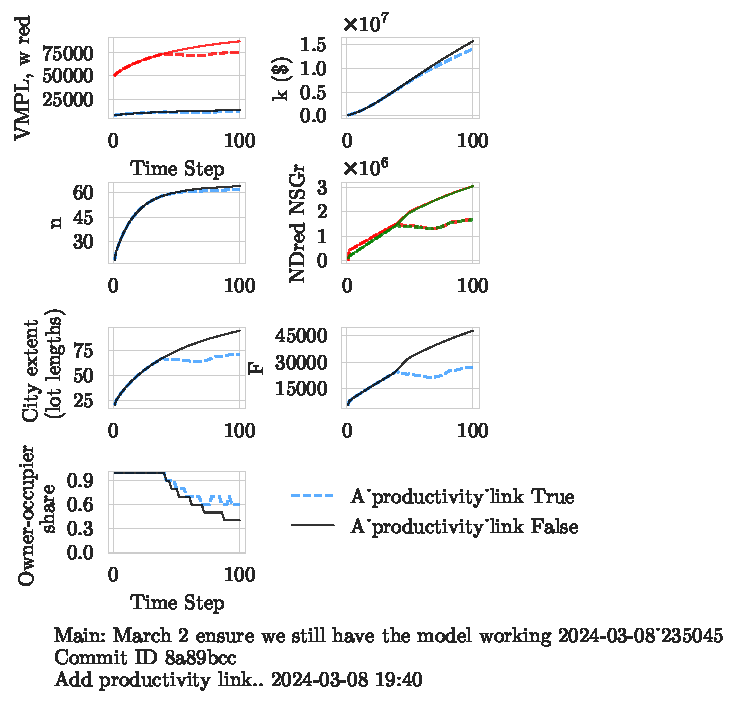
\includegraphics[scale=1, trim=.25cm 2cm .25cm .25cm, clip]{fig/productivity_link.pdf}
    \caption{Illustrating the impact of financialization on an urban economy}
\end{figure}
This is, to our knowledge, a new result, although it is consistent with fundamental urban theory and with The trends we see today in the urban system. The genuinely new component in our result is the formal  linkage of the financialized housing market to  urban productivity.

\subsubsection{Policy implication}
Assuming there are linkages of the sort we have illustrated here, it is important to ask if there are policy implications. Figure~\ref{Productivity_link_and_CG} indicates the effect of a 100\% capital gains tax on land speculation. 

\begin{figure}[h!tb]\label{fig-Productivity_link_and_CG}
    \centering
    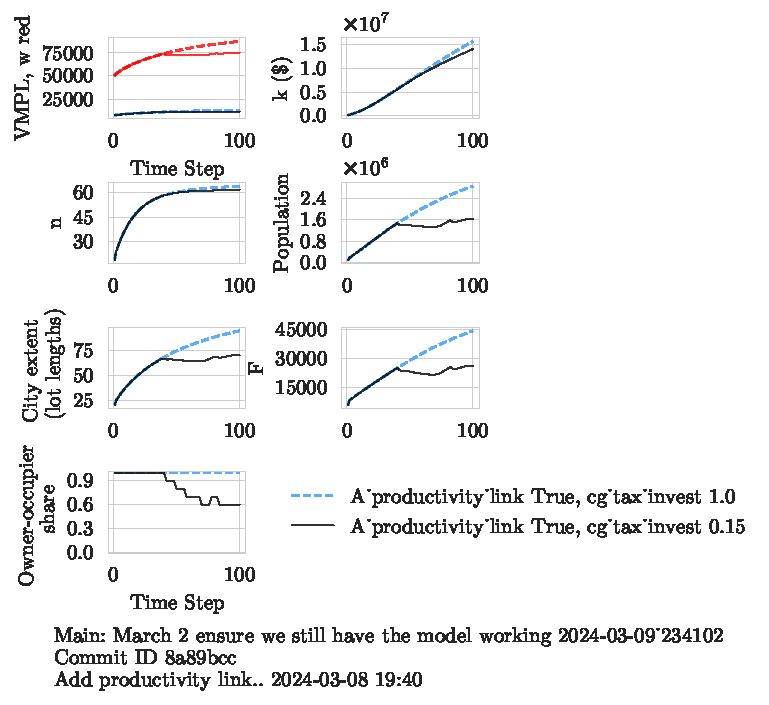
\includegraphics[scale=1, trim=.25cm 2cm .25cm .25cm, clip]{fig/Productivity_link_and_CG.pdf}
    \caption{The corrective effect of a capital gains tax}
    \label{fig:Productivity_link_and_CG}
\end{figure}

The figure shows that a 100\% capital gains tax on land speculation returns the city to its pre-financialization path, indicated by the solid line. In the housing market it has An `excess' effect, eliminating investor participation in the market, shown by the dashed line, and leading to higher rates of home ownership. 

% {\newpage\thispagestyle{empty}
% \vspace{-1.5cm}
\begin{figure}[h!tb]\label{fig-impact-channels}
%\vspace{-1cm}
\begin{adjustwidth}{-0.24\textwidth}{-0.24\textwidth}
\centering
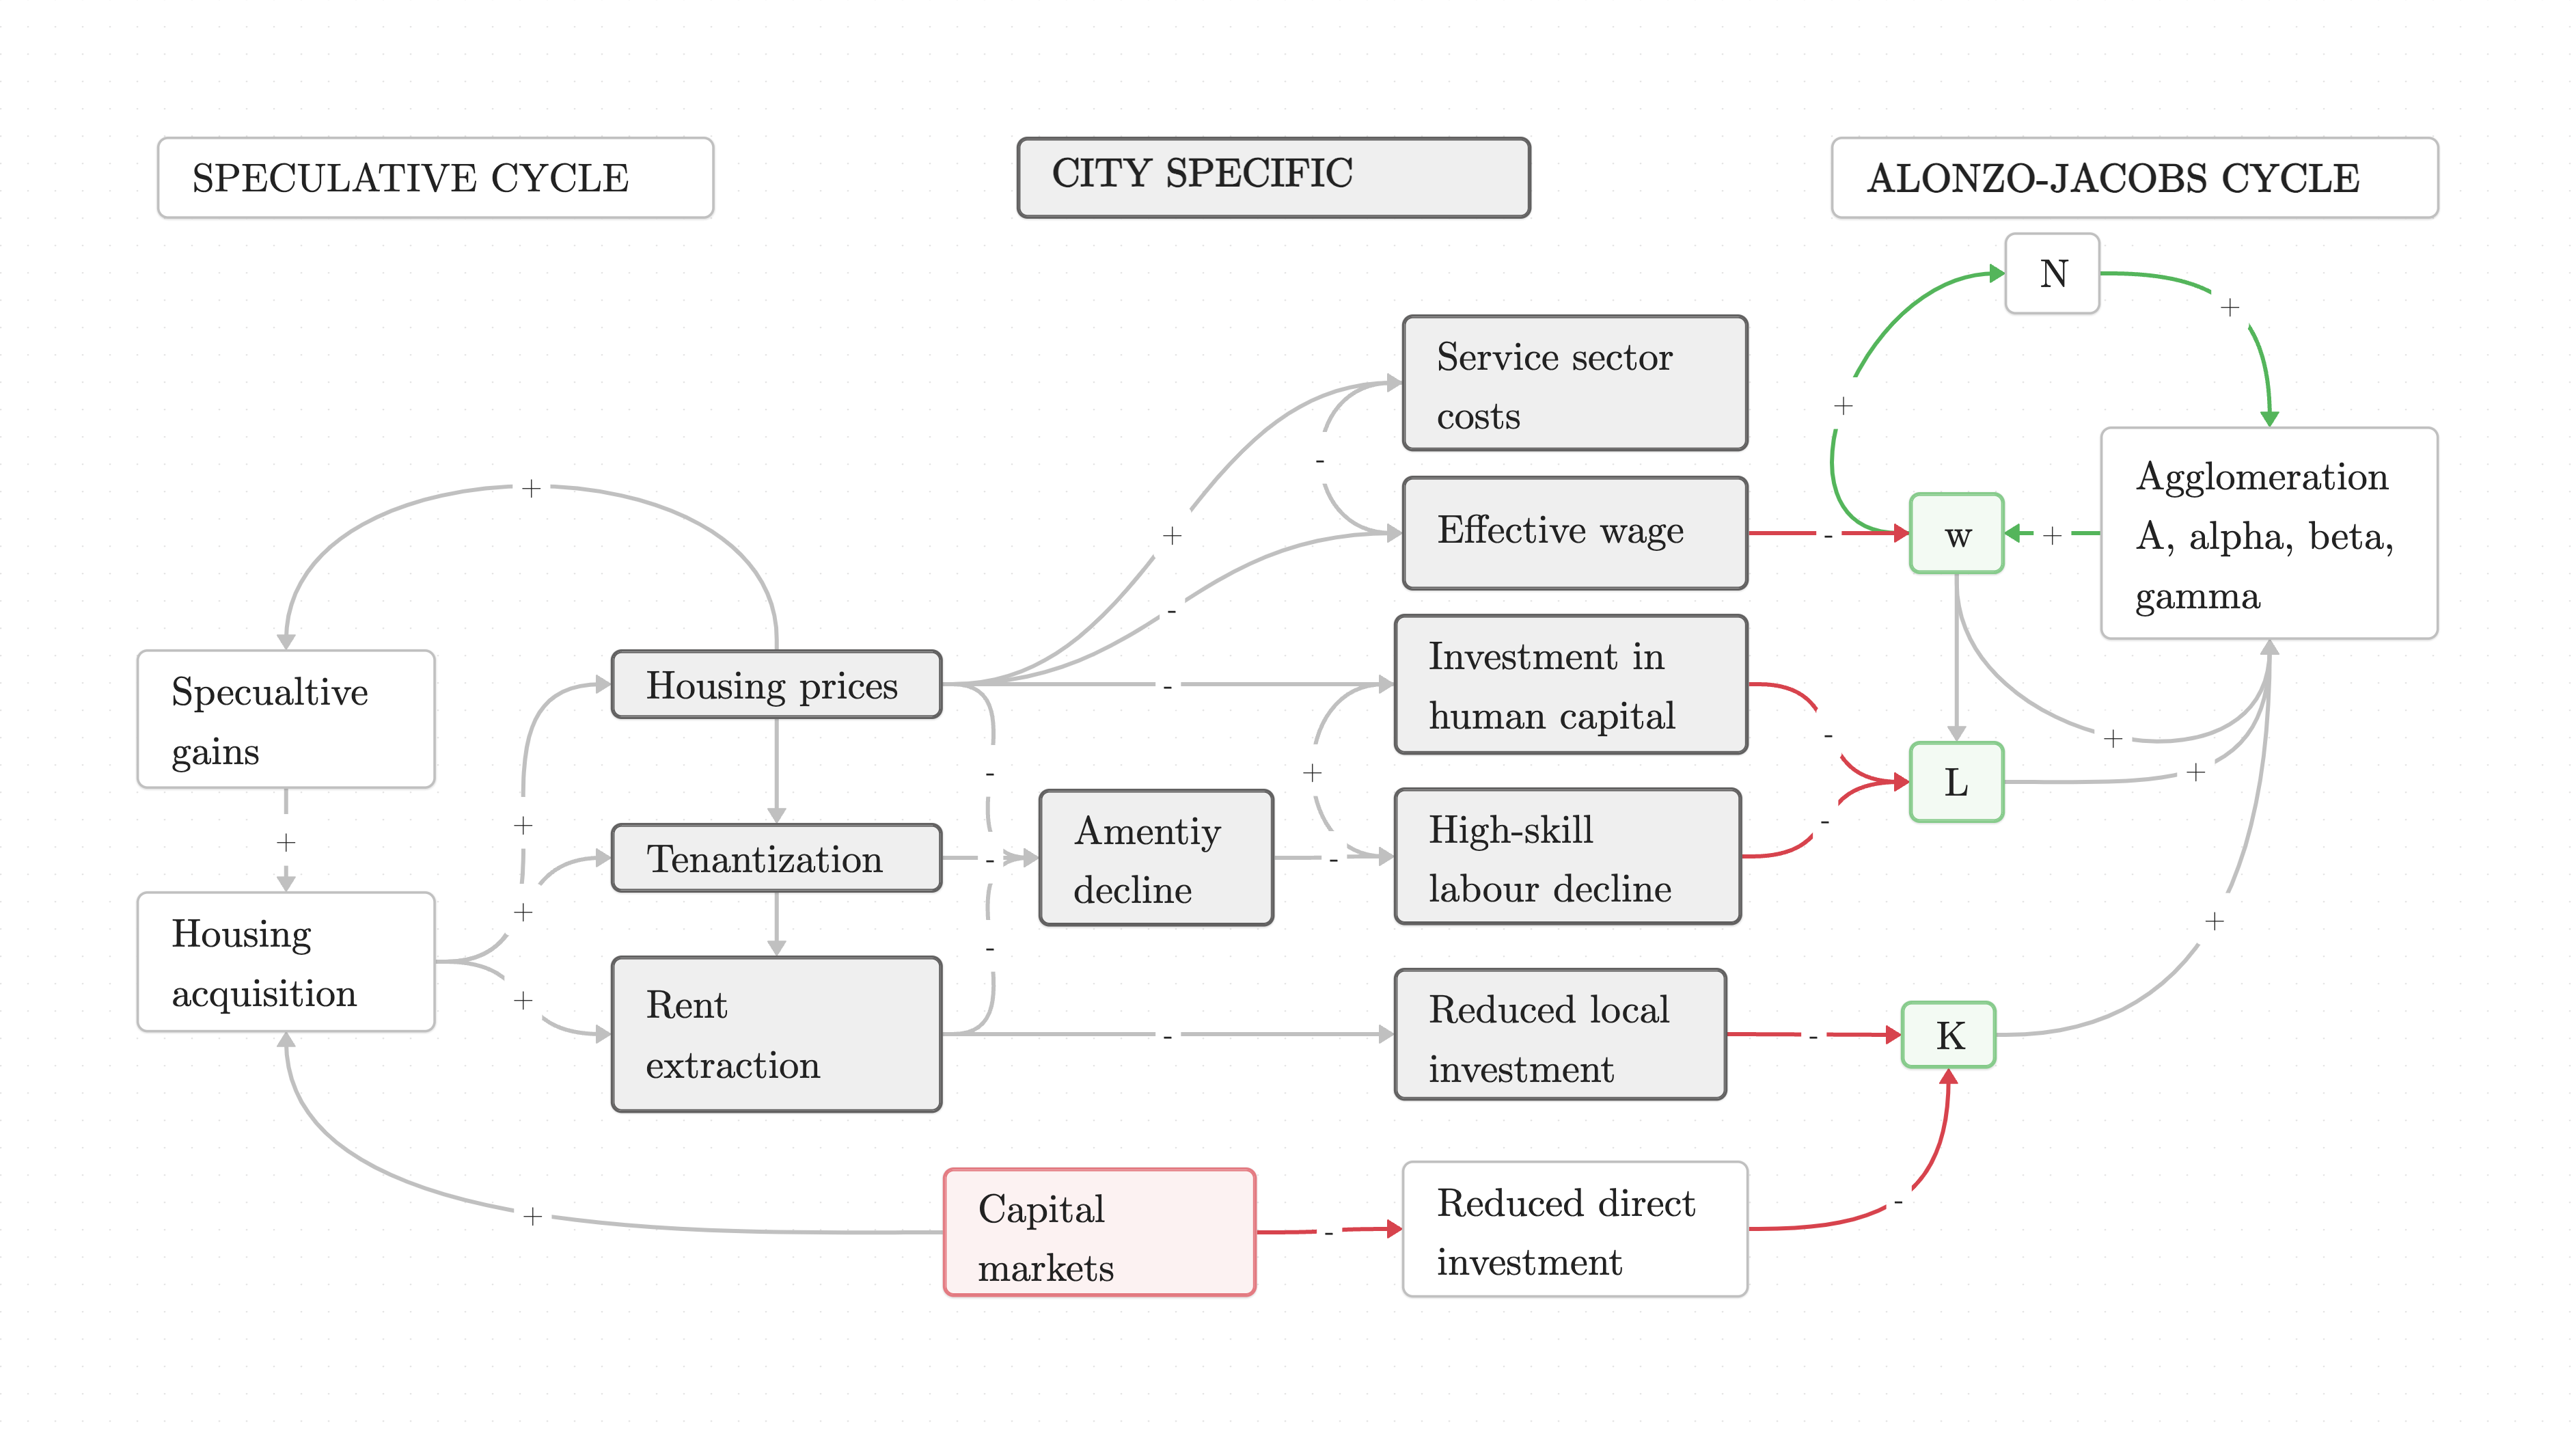
\includegraphics[scale=.15 ]{fig/impact-channels.png}%angle=90
\end{adjustwidth}
\caption{Impact channels relating financialization and urban productivity.}
\end{figure}
%}
 
%In addition, the variation suggests that that financialization may have an impact through multiple channels.  

% the channels through which the effect works are not clearly understood. 

% In particular, how the changes induced by financialization of the housing market might affect the fundamental productivity of the city has not been explored.



%{\color{red} In the next section we discuss potential linkages  with reference to the two dominant theoretical frameworks for understanding agglomeration effects, %. Second, it introduces the micro-foundations, the mechanisms by which agglomeration happens, drawing on the literature, and discussing how financialization might affect those mechanisms. Finally, in section~\ref{section-impact-channel-summary}, we summarize the primary linkages as they might appear in our model.} 

\section{Impact channels}
In the previous  section we  used our model to explore some  implications of a hypoithetical link between financialization of an urban housing market urban and the urban production economy. We now discuss in some detail the impact channels through which financialization. actually works. 

Understanding the mechanisms has considerable policy importance because it raises the possibility that there are several channels for public policy to enhance the positive effects of agglomeration. If the agglomeration parameters $A$ and  $\beta$ can be affected positively by policy choices, or perhaps negatively by trends such as financialization,  governments may be able to significantly increase social wealth and well-being. We discuss potential channels more fully in the following sections. 

Determining the importance of the various impact channels in general or for a specific city is an empirical problem well outside the brief of this thesis. Tests in the universe of the model, however, can lay the foundation for later empirical work. Identifying channels through which the policies or trends might affect productivity is important for this work because by introducing hypothesized linkages into our model explicitly, we have created a framework for systematically testing the model's sensitivity to a range of policy interventions. 

Figure~\ref{fig-impact-channels} illustrates some of the channels through which the financialization of housing might impact city productivity. 
In the figure, the production sector is on the right, the processes occurring within the city are central, and the speculative intervention in the housing market is to the left.  \footnote{The figure only shows some of the links and feedbacks we discuss. It is not our intent in this chapter to provide  a comprehensive discussion of any of the linkages we examine. Each of the linkages shown or mentioned warrants extensive research, and for most even a brief literature search will reveal many related papers.} 


In the upper right, we show the \gls{Alonzo-Jacobs cycle}, described in Chapter~/ref{chapter-model}. In it, the strength of the agglomeration effect determines productivity, which drives wages, which determines population which feeds back to agglomeration. In our model, anything that affects productivity must affect this cycle directly or indirectly.  We show the effect of interventions or financialization on productivity primarily through their effect on wages, labour supply and capital supply. %making it indistinguishable from the Jacobs model at the urban level. 

 %Identifying these linkages is important but it is complicated on at least two levels. First, the micro-level mechanisms driving productivity gains in the production sector, themselves are not well understood.  Second, the linkages between urban productivity and financialization have not been established.  

% {\color{red}
% \section{Mechanisms by which Financialization affects Productivity}
% The literature identifies several possible mechanisms by which financialization might feed back into affecting the productivity of the city. ANY THING OVERARCHING WE CAN SAY ABOUT THIS?LATER, IN CONCLUSION YOU SAY : To do this, we identified the housing market channels through which the changes in ownership might be transmitted through the economic and social body of of the city to the Alonso-Jacobs cycle, where agglomeration effects generate wealth.  }

\subsection{Reduced capital stock}

Marxist theorists \cite{lefebvreRevolutionUrbaine1970, harveyClassmonopolyRentFinance1974, harveyUrbanProcessCapitalism1978, christophersRevisitingUrbanizationCapital2011} have argued that finacialization diverts capital investment from productive investment to financial enterprises. 

This direct effect is illustrated at the bottom of Figure~\ref{fig-impact-channels}, where capital markets can divert capital from the productive activities on the right to speculative activities on the left.  Switching happens in response to the relative rates of return on the two sides. We have assumed a perfectly elastic supply of capital to firms and speculators, leaving modelling more complex and possibly more realistic capital markets to later work.  We allow the rate of return on housing investment to rise in response to city growth, however, attracting speculative investment. We could also simulate a falling rate of return on non-housing investment by reducing the cost of capital to investors or by inhibiting the rate of growth of capital on the production side in response to rising investment in housing purchases. % adjK



\subsection{Local investment}

Financialization may reduce the amount of local capital available, raising the cost of capital in the city. 
There are at least two mechanisms by which local investment capital may be affected. First, if increased tenantization and rent extraction reduce household wealth, we would expect household investment to decline. The decline would probably be correlated with a decline in direct investment, amplifying its effect. Furthermore, this channel would act very slowly and persist after an initial round of speculative activity. 

Second, because private production is complemented by public infrastructure, it is possible that the tenantization for the city would lead to declining municipal investment in public infrastructure. It is known, however, that municipalities generally spend less on tenants and collect more revenue per capita from rental as opposed to owner-occupied housing, so tenatization might lead to rising pressure for infrastructure expenditure.  We can capture these effects by linking the owner-occupier ratio to capital stock. A more detailed approach would explicitly allocate some of the municipal taxes to increasing the agglomeration parameters. 




\subsection{High-skill labour decline}

 Speculation and rising housing prices that result in tenantization will make a city less attractive to highly skilled labour, making it more difficult to attract or hold people with the specific adaptive skills Glaeser and Saiz \cite{glaeserRiseSkilledCity2003} identified. Slowing in-migration or increasing out-migration of the more skilled members of the labour force  will \textit{ceteris paribus} reduce the effective supply of labour. 
Liu et al \cite{liuImpactUrbanHousing2023}, for example, found for China that and increase in urban housing prices has a crowding-out effect on labour mobility.  Duffy et  \cite{duffyRisingHousePrices2005} found that for Ireland that rising house prices, by discouraging potential migrants, could significantly reduce the growth potential of the economy, shifting the balance of labour market growth from employment to wages, with a consequent deterioration in competitiveness. %Anecdotal evidence comes from comes form the frequent news stories about which cities are most livable: low housing prices are almost always an important element in the measures used. (we omit the link form  housing prices to high-skill labour. 

Althobaiti et al \cite{althobaitiHousingPricesSkills2021}  show that with gentrification, high-level cognitive skills are getting closer to the city center in response to the increase of median housing prices while low-level physical skills got further away.  Gentrification can be seen as trend opposing tenantization. The effects of tenantization, neighborhood decline and disinvestment, which Cornelissen and Jang-Trettien \cite{cornelissenHousingContextNeighborhood2023} point  are more common than gentrification in low-income neighborhoods, are likely to be opposite of the effects of  gentrification.

The reduction might be offset by importing human capital, though immigration or rising wages for talent in the city. Florida\cite{floridaCompetingAgeTalent2005, floridaCreativeClassEconomic2014} has suggested that urban growth is strongly linked to the ability to attract talent. 

We can introduce this channel by making  the labour elasticity of output in the Cobb-Douglas function, $\beta$, depend on the home-ownership ratio.  


\subsection{Reduced investment in human capital}

There is a vast literature on investment in human capital. 
Growth theory associates increasing returns to scale in the industrial sector or at the national level with increasing effective human capital, which grows faster than the labour supply as a result of increased education, as we described in Chapter~\ref{chapter-growth} section~\ref{section-growth}. 
Growth theory suggests that the growth of human capital is  a major driver of productivity.  At the national level, Solaki \cite{solakiRelationshipEducationGDP2013} demonstrates a causal relationship between education and growth, and that tertiary Education should be considered as an exogenous variable.  Empirical results for Bangladesh \cite{islam2007relationship}show evidence of bidirectional causality between education and growth.  Among others, B\"uchler et al have recently confirmed the important of human capital growth for urban growth.

There are at least two mechanisms by which investment in human capital may be affected indirectly by financialization. The most direct is by reducing household incomes The effect may be different for different parts of the population. Increasing housing prices increases the wealth of owner-occupiers. this wealth effect may result in increased spending on education for offspring. Increased housing costs for tenants, on the other hand,  may result in reduced human capital investment.\footnote{Glaeser and Saiz found evidence for skill upgrading in declining cities, which suggested to them efficient investment in less skilled workers is a key adaptive/growth mechanism. If powerful enough this effect might offset some of the negative impacts of financialization we has suggested.}  

Less directly, we suspect financialization will increase the cost of living through, for example, increasing labour costs in the service sector. This results in a reduction of the effective wage, also reducing income available for human capital investments. Rent capture leading to reduced local capital of reinvestment in human capital might reduce the adaptive capacity of a city's population.

We can simulate some human capital effects simply by making a link from the home-ownership ratio to the productivity parameters  $\beta$ and $A$. 



\subsection{The effective wage}

Purchasing power depends on the money wage and on the price level. inflation coming from the right side of the figure will reduce the effective urban wage, which Lobo et al. find is one of the determinants of growth. 

 Rising housing prices and rising rental prices reduce the purchasing power of city dwellers in more than one way. In addition to the direct effect, the rising housing costs make other goods and services more expensive. The wage of the Barista must go up, so the cost of a coffee has to rise. Bookstores may close, reducing the neighbourhood amenity level. 
 
 Local amenities may also be affected. Urban amenities  are part of the incentive for choosing city life for many, and any decline in amenity will have the same qualitative effect as a decrease in the wage. The size of the effect will vary because people's tastes differ. 


 General financialization may also reduce the bargaining power of labor, as Tomaskovic-Devey and Lin argue \cite{tomaskovic-deveyFinancializationCausesInequality2013}, reducing wages.\footnote{Tomaskovic-Devey and Lin point to a shift in behaviour of non-finance firms away from production and non-financial services and toward financial investments and services. This shift, they argue,  has led to lower employment, income transfers to executives and capital owners, and increased inequality among workers \cite{tomaskovic-deveyFinancializationCausesInequality2013}}
%In the second part of the chapter we implement several of the mechanisms and share results. 

% VERY INTERESTING \cite{buchlerImpactHumanCapital2024} in areas with elastic housing supply, the positive demand shock leads to the construction of more housing, a larger labour force, and, thus, moderate wage growth. In contrast, in areas of low housing supply, the positive demand shock has a limited impact on new housing construction and the urban population. Human capital gets capitalised into higher home prices, hindering urban growth.

\subsection{The amenity channel}
Rent capture might influence the concentration of educated personnel by reducing the diversity and amenity of cities, making urban living less attractive, reducing labour supply, or raising its cost.



\subsection{Impact on the service sector}
Rising housing costs at the centre of a city would tend to push low-wage workers to the edges, increasing their transportation costs, putting further upward pressure on wages, and increasing the costs of all amenity services that rely on lower-cost workers.

\subsection{Small cities may provide clues about impact channels }\label{sec-fig-residuals}
Interestingly the residuals or unexplained components for smaller cities are much larger than they are for large cities, as Figure~\ref{fig-residuals-lobo} from Lobo et all \cite{loboUrbanScalingProduction2013} illustrates. The observation suggests that clues about the mechanisms may be found by examining smaller and mid-sized cities and that potential policy impacts may be greater for these cities.

\begin{figure}[h!tb]
\centering
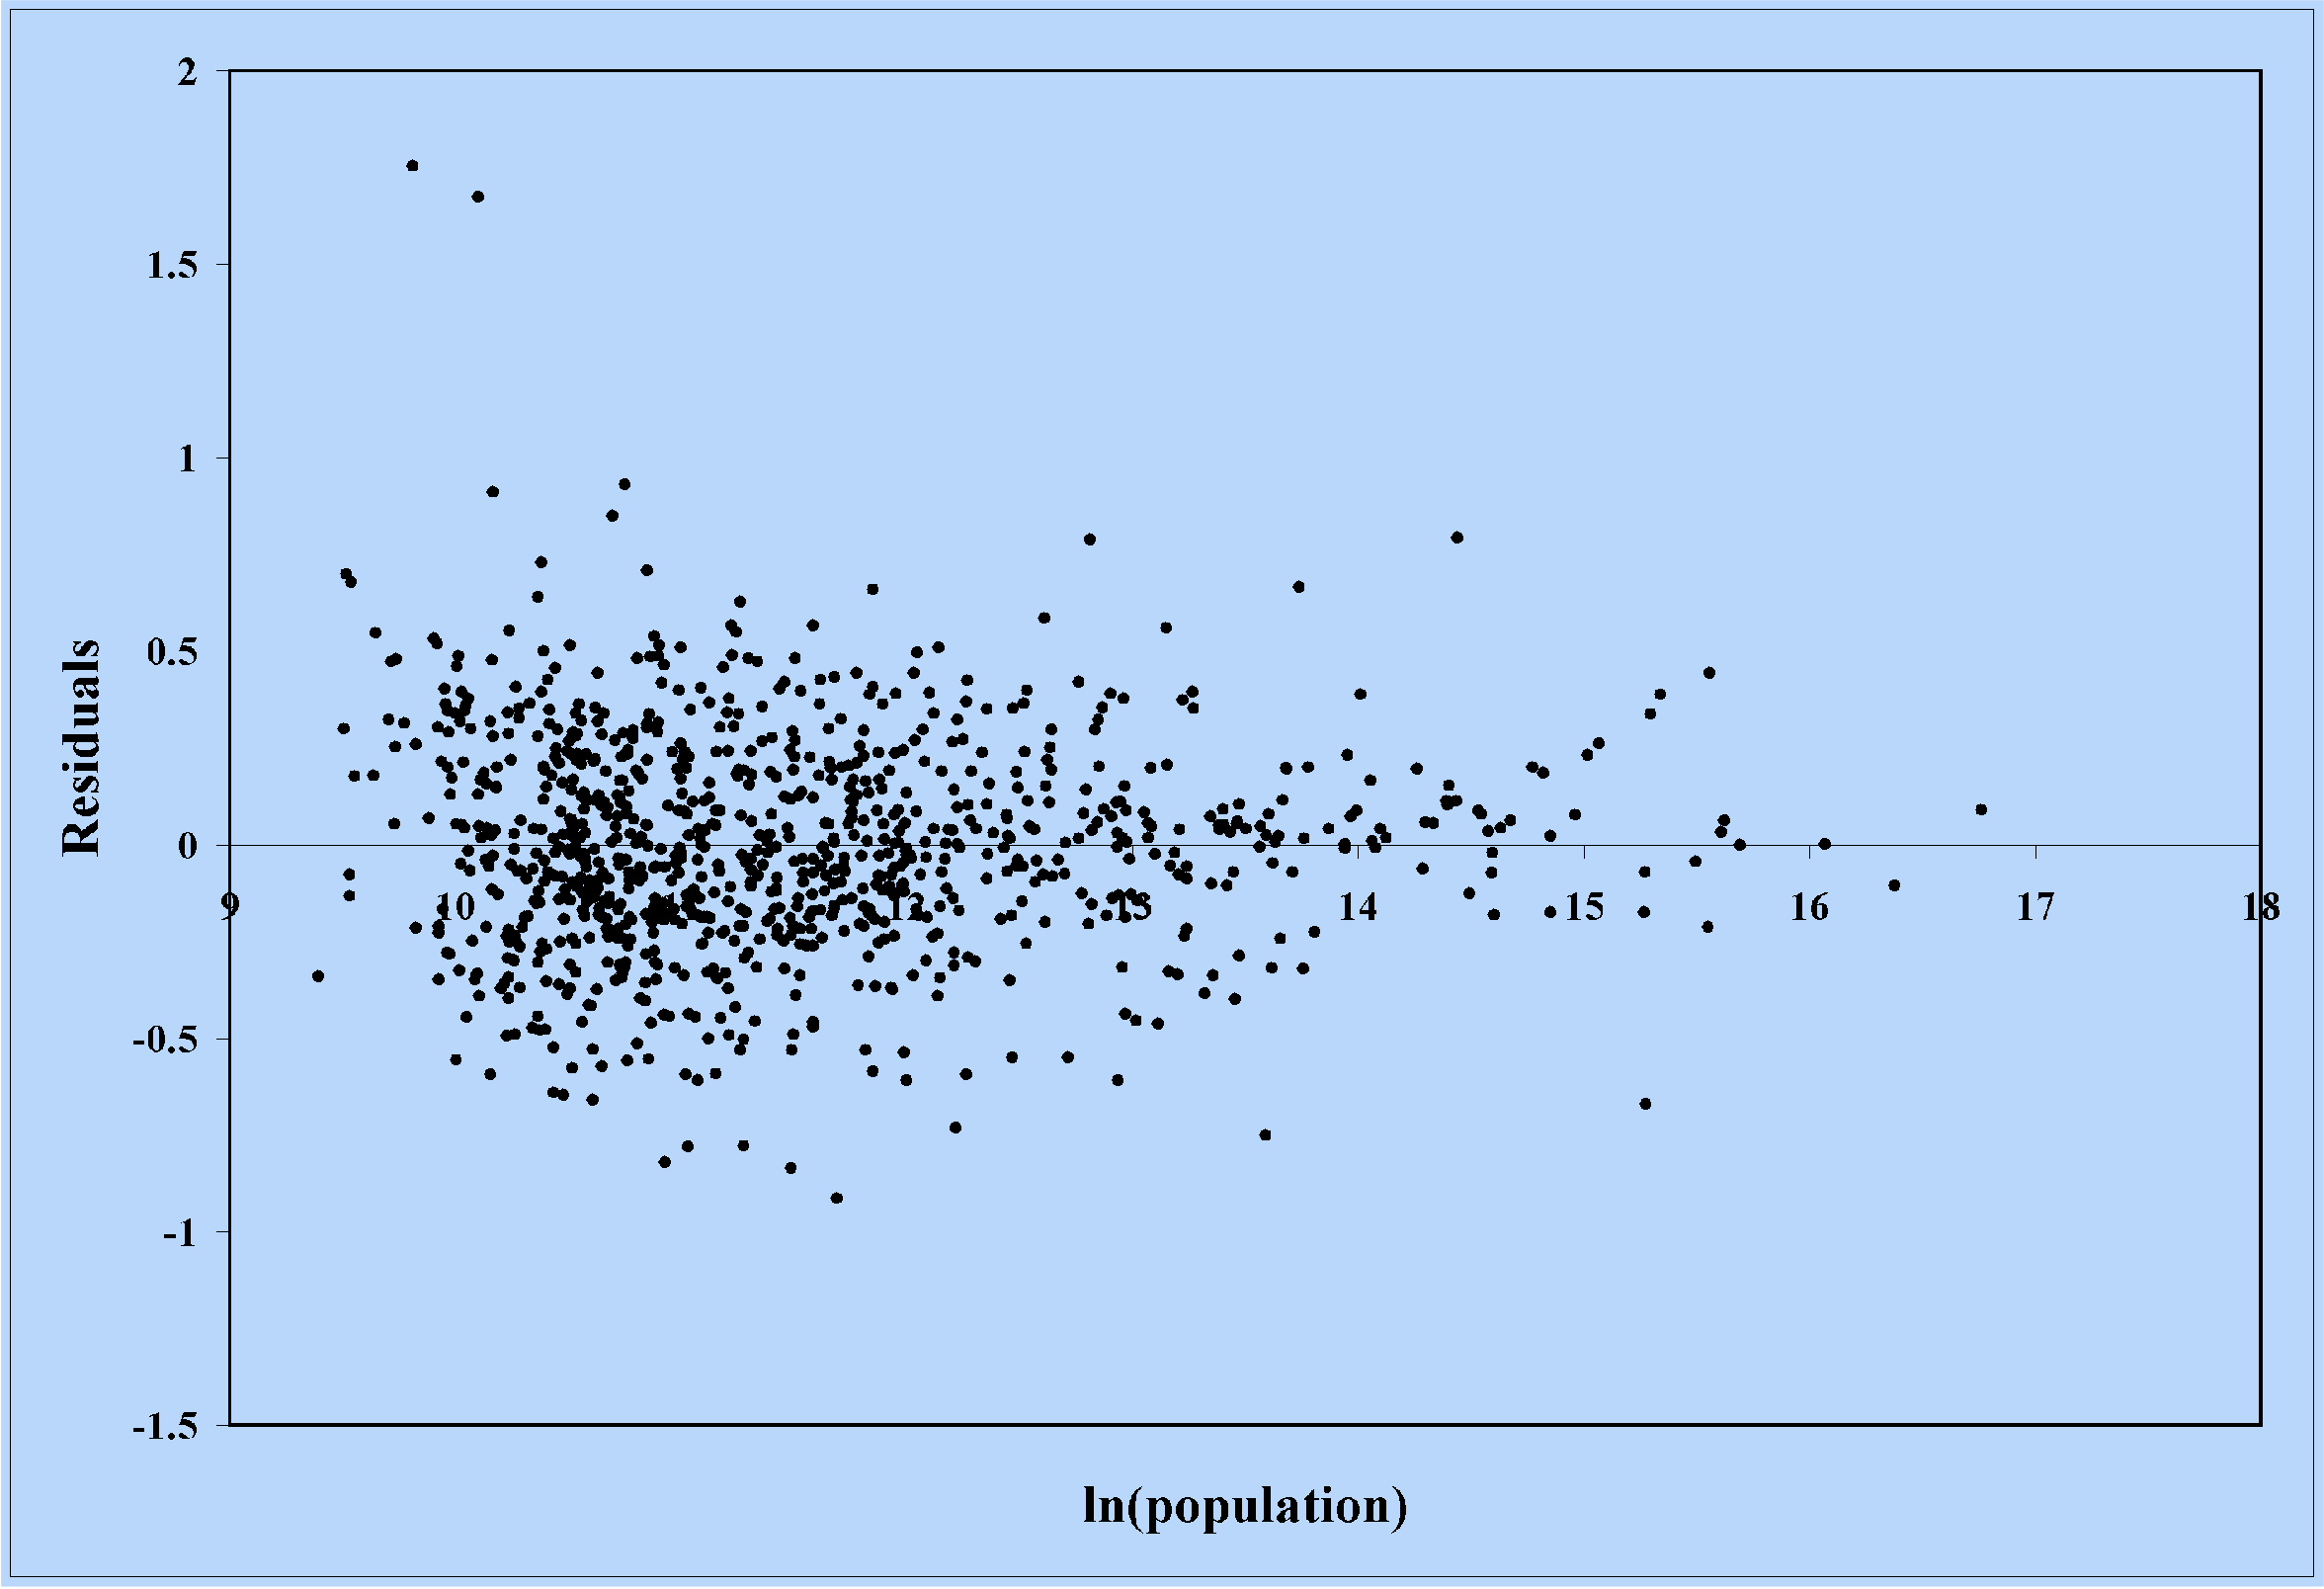
\includegraphics[scale=0.30]{fig/residuals-lobo.png}
\caption{Residuals from regressing ln(total wages) on ln(population) using data for all 943 urban areas of the United States showing larger unexplained components for smaller cities. \cite{loboUrbanScalingProduction2013}.}
\label{fig-residuals-lobo}
\end{figure}



\section{Conclusion}
 The dominant effect of financialization is to shift ownership of housing from occupiers to owners of financial capital. In this chapter, we have described a number of the most likely channels through which the effect of financialization on ownership  might be transmitted through the economic and social body of of the city to the Alonso-Jacobs cycle, where agglomeration effects generate wealth. The list is not complete but it provides a framework for testing the model's sensitivity to a range of policy interventions and lays the foundation for empirical work.  

The key result is that both our analysis and our simulations indicate that finacialization   can affect urban productivity. 

Financialization may also affect the industrial structure and the settlement pattern as well, but we defer extending the model to include these effects. Our focus in this chapter has been limited to examining possible channels through which the housing market financialization is likely to affect to affect the productivity of a city. We conclude, based on our analysis and simulations,  that the unrecognized impacts of financialization of the urban housing market may have extremely serious effects on the economy as a whole.

% We have modeled the relationship between ownership and the inputs to the aggregate production function described in Chapters~\ref{chapter-growth} and \ref{chapter-model}. 

% {\color{red}
% Essentially, the discussion in this chapter has guided and helps explain the policy experiments we have conducted. MAYBE ADD A FINAL SENTENCE PULLING IT ALL TOGETHER?}






\chapter{Amenity}\label{chapter-amenity}
%Future work
Our model has been developed to be extensible. In the development of the model we have constantly considered how to integrate the most likely and most useful extensions. In this chapter, we briefly describe a number of those extensions, what we might learn from them, and how we propose to incorporate them,



\section[Amenity]{Incorporating amenity}\label{section-amenity}
% from Ricardo_Rent_and_Roemer_3.tex
In our base model,  an urban wage premium is the only labour attractor: it an the transportation cost determine land values. In our base version therefore, we have set the level of amenities to zero  so we can focus on the productivity effects. The wage premium provides a reason to find housing in the city and to travel to the city centre to work. Housing choice, however, is always the purchase of a bundle of characteristics such as location, building space, yard, local density and local \glsdisp{amenity}{amenities}. Stegman  found that ``a large majority of families who have recently moved to the suburbs are more concerned with neighborhood quality than with accessibility to other parts of the metropolitan region.'' 
``There is evidence that the amenities offered by a city enhance its growth \cite{clarkAmenitiesDriveUrban2002, falckPhantomOperaCultural2011a} and that amenity effects themselves scale superlinearly\cite{kraemerCulturalSustainabilityUS2022}. 



Kaufmann et all \cite{kaufmannScalingUrbanAmenities2022} investigated the general statistical patterns in the quantity and spatial distribution of different urban amenities including public spaces and institutions as well as businesses, which all provide different services to urban populations, such as restaurants, parks, or universities.  They argue that amenities are   in fact central for generating and supporting economic agglomeration effects, attracting investment to ``developing neighborhoods, promoting economic growth, supporting innovation clusters and facilitating businesses linkages.'' 
They show that the aggregate quantity of amenity infrastructure (not amenity supply)  in an urban area scales sub-linearly with population size across US metropolitan areas.\footnote{When they disaggregate, however, they find that for approximately 74\% of amenity types, they cannot reject linear scaling. Four percent exhibit super-linear scaling. They list take-away restaurants and travel agents in this range. Sub-linear scaling is associated with libraries, universities, and movie theatres.} This strongly suggests there are scale economies in amenity provision.\footnote{The model they use is the same as the one used to demonstrate that a scaling law holds for urban GDP. Instead of GDP, however, the dependent variable is a measure of amenity density based on data extracted from a unique new Google Places dataset, Google Places API (2012).} 


The amenities offered by a city can be seen as a form of non-market, non-monetary income \cite{kaufmannScalingUrbanAmenities2022}.  The non-market component of household incomes affects choices. Greater consumption amenities in a city will make workers willing to accept lower wages or higher rents. For firms,  lower wages mean lower costs. Thus,  higher amenity levels may lead to lower money wages as workers trade amenity for money income. With lower wages, more workers can be hired leading to higher output and a larger population. \cite{pugaMagnitudeCausesAgglomeration2010}. 
When positive urban amenities prevail, rents and housing prices will be higher in larger cities, but wages may be unaffected \cite{robackWagesRentsAmenities1988, dalmazzoAmenitiesSkillbiasedAgglomeration2011}.
%localized productive advantages will make firms willing to accept higher wages and higher rents  


%It involves budget allocation. If we hold the housing budget constant and add an explicit urban amenity, other variables must adjust. 
% Higher wages make residents better off whereas higher rents make them worse off. Thus, 


%.  This helps disentangle the consumption amenities from the productive advantages of big cities.


In our base model,  To introduce amenities we can simply add an amenity value $A$ to the estimated value of any home. The value can depend on location, allowing for `better' and `worse' neighbourhoods,  and it can be made to depend on household attributes: a family with children might value a neighbourhood with a school or a park more highly. 

For some households, the amenity of an area may depend on the density of the city or of certain types in a neighbourhood. This is a social agglomeration effect that may work in addition to the agglomeration effect on production (\cite{gurwitzCatastrophicAgglomeration2019}) that we have already considered. There are also agglomeration effects in consumption goods. Larger consumer markets support more variety in goods and services. This variety allows a greater range of preferences to be satisfied. A larger city may have more production sectors and a larger array of consumer services, increasing the value received from a given income.  These closely related but different effects can be modeled by introducing an amenity term in various ways 

The amenity-induced rise in housing prices may absorb what would otherwise be consumption expenditure on other goods. Residents might accept smaller housing units for access to urban amenities. \footnote{Some costs may fall with agglomeration. There is evidence of a strong negative correlation between the total energy consumption of a city and its overall urban density \cite{NewmanPeterJeffrey}. Larson et al. \cite{larsonEnergyImplicationsCity2015} show that per-capita energy use is relatively invariant to city size when growth is driven by wages but falls modestly with growth induced by rising amenity.} In any case, there will be distributional effects as amenities play a larger role in urban agglomeration. Property owners will capture increased land rents. If amenities are funded out of taxes, the burden falls on all residents, since property taxes are very roughly related to housing consumption, but the land rents are captured by institutional owners as well as owner-occupiers and not by tenants.
÷

%\glspl{amenity}, or non monetary income it another form of wealth,See Kaufmann et al. \cite{kaufmannScalingUrbanAmenities2022}.  and it is %, are however, an important feature of the urban system. 
% We have intentionally suppressed amenity but can add it it simply.
% (ownership effects, produtivity spilllovers, - table where you show them in the static and dynamci case with amentity)
% 2 classes of exploratin of the model in the past tho chaptered
 This sectionr sketches an extension of the model to study include \gls{amenity} and suggests how it might affect results. 

 
%To understand amenity in our model, we need to understand it's relationship with growth, productivity, and agglomeration.
\subsection{Modelling amenity}
Amenity effects can be introduced in a variety of ways. hey might work though An economics might prefer to introduce amenity as a good in the utility function of agents. It might then depend on the size of the city, the size of an amenity-producing sector, the specific amenity-generating infrastructure provided by the city through taxes,  or neighbourhood effects. Each of these would take a different functional form. In our model agents are represented by their demand for housing, so the same terms would have to be introduced into the bid function. In the utility framework, bids are simply derived from the utility function, so the two approaches are equivalent. The virtue of using the utility framework is that it begins with the question, "What do people want?" rather than "What do people do?" The first question is more productive if we want to identify different amenities that might matter.

\subsubsection{Through household utility}
 The most direct way to incorporate agglomeration amenities is to include what might be called a \gls{utility premium} for urban dwellers as non-monetary location income $\mathbb{A}(d; N), \die{\mathbb{A}}{N}> 0), \die[{\mathbb{A}}]{d}< 0)$ depending on distance, $d$ from the centre and urban population $N$. The second term can incorporate local amenities as well. A simple linear (indirect)\footnote{The indirect utility function is a function that depends on income and prices rather than goods and services.  Income does not generate utility, but it does generate utility indirectly' because it enables people to purchase goods and services.} utility function specified on broad income (net wage plus locational amenity) is convenient for illustration:

\begin{equation}VU(w,A)= \psi+ \omega-cd + \mathbb{A}(d; N) - T(d))
\label{eqn-u}
\end{equation}
where $w$  is an urban wage p, $T(d)$ is transportation cost from the centre to $d$.
\footnote{\cite{anasUrbanSpatialStructure1998} shows that a linear transportation cost will not  hold if congestion declines  with $d$.} 
 In most versions of the Alonzo model the `wage premium' is simply given in the urban wages and there is no amenity term. 


%\footnote{wage income, if all income goes to housing, or the share of wage income going to housing services.   (If we use a Cobb-Douglas utility function we would just replace $w$ with    $\alpha Y$, where $Y$ is household income and $\alpha$ is the share of total income. } Let  $T(d)=td$ be transportation cost with  $t>0$. 
 
\begin{figure}[t!b]
\begin{center}
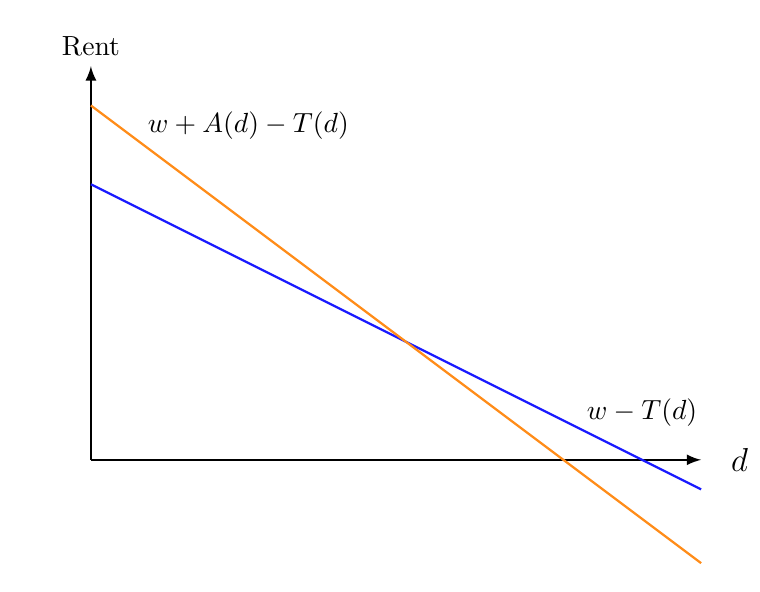
\begin{tikzpicture}[scale=.5]
\def\bndmax{5}        %https://tex.stackexchange.com/questions/68462/filling-a-complex-region-with-tikz
\def\bndmin{0.2}
\def \n {10}
\def \m {15.5}
\def \t {.5}
\def \th {1}
\def \w {7}
\tikzset{func/.style={thick,color=blue!90}}	
\draw [thick, latex-] (0,\n)node[above] {Rent}--(0,0);
\draw [thick, -latex] (0,0)--(\m,0)node[right=.25]{\large $d$};
%\foreach \xi in {0,..., \m} \draw (\xi,0)--(\xi,-.1)node[below=1]{\small$\xi$};
%\foreach \yi in {1,...,\n} \draw (0,\yi)--(-.1,\yi)node[left]{$\yi$};
%%\foreach \i in {1,4,9,16} {
	\draw[func,domain=0:\m] plot [samples=200] (\x,{\w-\t*\x});
%	\draw[func,domain=0:\m, dashed] plot [samples=200] (\x,{\w+\azero-\th*\x+\aprime*\x});

\node at (14,1.2){$w-T(d)$};
\def \azero{2}
\def \aprime {-.25}	
\tikzset{func/.style={thick,color=orange!90}}	
	\draw[func,domain=0:\m] plot [samples=200] (\x,{\w+\azero-\t*\x+\aprime*\x});
\node at (4,8.5){$w +A(d)-T(d)$};
%\node at(-.8,2) [left]{base $2^1=$};
%\node at(-.8,1) [left]{$2^0=$};
%\draw[dotted] (0,2)--(1,2)--(1,0); 
 \end{tikzpicture}
\end{center}
\caption{Rent profile with amenities}
\label{fig-amenity}
\end{figure}

 This model can produce variations on the standard result in the Alonso model. Figure~\ref{fig-amenity} illustrates a linear amenity function, $\mathbb{A}(d|N)= a-b*d$, that is convenient for illustrative purposes.  It shows how a particular amenity function might affect the rent profile, and hence city size and it allows simple experiments with the effect of increasing population on city size, wages and rents. 

In this case, amenity falls below zero in the outer regions of the city and, the geographical size of the city will be smaller. With a linear function, this happens if $\frac{a}{b} < \frac{w}{t}$. (a smaller city would have a secondary effect on wages, since with fewer workers' marginal productivity would be higher and therefore wages would rise. This would partially offset the initial decline in population.)

 There would be a band of land around the city with negative amenity for commuters.\footnote{The very simple graphical result rests on several assumptions - no other housing expense, housing all the same size, wages all equal, preferences identical, transportation costs.}

The far more likely case is that $A(d) > 0$ when $w-T(d)$ falls to zero. In this case there is a band of residents around the city, outside of the population commuting to work. They do not travel to work,  do not collect a wage, but still enjoy the amenity of being close to a city. This might be a population of retired persons enjoying occasional visits and healthcare facilities.


\subsubsection{Neighbourhood amenity}
In Figure~{fig-amenity} the source of the amenity is at the centre of the city. We can easily imagine an amenity profile that is high for some neigbourhoods and lower for others, as in  In Figure~\ref{fig-amenity2}. The jagged area below the orange line is rent accruing to landowners. The variable rent comes not from a desire to be close to the source of the wage income but from household demand for local amenity.  

\begin{figure}[tb]
\begin{center}
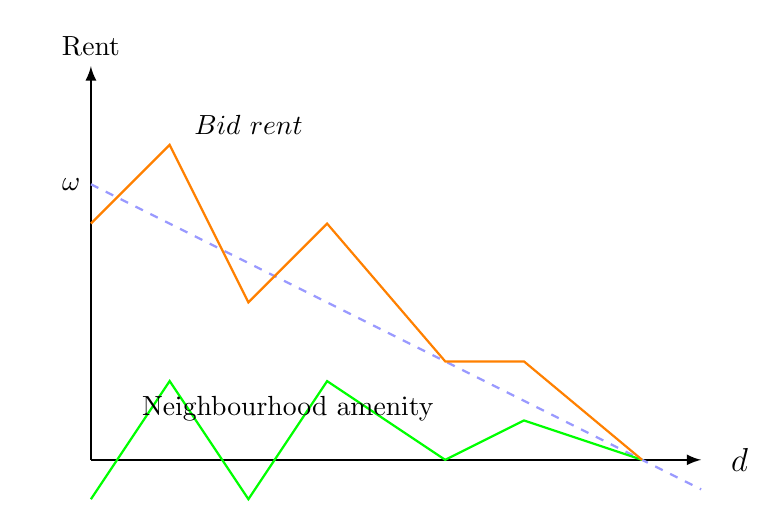
\begin{tikzpicture}[scale=.5]
\def\bndmax{5}        %https://tex.stackexchange.com/questions/68462/filling-a-complex-region-with-tikz
\def\bndmin{0.2}
\def \n {10}
\def \m {15.5}
\def \t {.5}
\def \th {1}
\def \w {7}
\tikzset{func/.style={thick,dashed, color=blue!40}}	
\draw [thick, latex-] (0,\n)node[above] {Rent}--(0,0);
\draw [thick, -latex] (0,0)--(\m,0)node[right=.25]{\large $d$};
% Basic Bid rent,
\node at(-.5,\w) {$\omega$};
\draw[func,domain=0:\m] plot [samples=200] (\x,{\w-\t*\x});
%NEIGBOURHOOD AMENITY
\draw [thick, green] (0,-1)--(2,2)--(4,-1)--(6,2)--(9,0)--(11,1)--(14,0);
\draw [thick, orange] (0,6)--(2,{7-2*.5+2})--(4,7-4*.5 -1)--(6,7-6*.5+2)--(9,7-9*.5)--(11,7-11*.5+1)--(14,7-14*.5);
\node [] at (5,1.3){Neighbourhood amenity};
\def \azero{2}
\def \aprime {-.25}	
% \tikzset{func/.style={thick,color=orange!90}}	
% 	\draw[func,domain=0:\m] plot [samples=200] (\x,{\w+\azero-\t*\x+\aprime*\x});
\node at (4,8.5){$Bid\ rent$};
%\node at(-.8,2) [left]{base $2^1=$};
%\node at(-.8,1) [left]{$2^0=$};
%\draw[dotted] (0,2)--(1,2)--(1,0); 
 \end{tikzpicture}
\end{center}
\caption{Rent profile with neighbourhood amenities}
\label{fig-amenity2}
\end{figure}
Financialization might or might not affect neighbourhood amenity. If it does it might have its effect by changing the ownership mix.

\subsubsection{Public provision of amenities}

Previous sections suggest amenities may work as a wage subsidy, potentially increasing output. Since employers will not willingly pay for urban amenities, some amenities may be financed publicly. It is common to introduce the cost of generating amenities as a tax on residents.  Since public amenities may be \glspl{public good} in the economic sense, the municipal government may be able to achieve significant wage economies with a small public expenditure.

A simple way to incorporate publicly provided amenities to make an amenity function that proportional to a fraction of public revenue, which is a fraction $\tau$ of the land value when municipalities depend on property taxes. Assuming a uniform property tax rate, total property tax revenue in a circular city are approximately $\tau(\phi+2/3 \omega)\pi \frac{\omega}{c}^2$. We can therefore include in the buyer's maximum bid function a fraction if this value. Property investors would not include this amenity component, but it would affect their decisions because amenity raises their net rent.

Notice that because amenity raises property values, in Ontario it does not raise tax revenue because the property tax rate is adjusted to balance the budget. This creates perverse incentives for municipalities \cite{blaisPerverseCitiesHidden2011}.


\subsubsection{An amenity sector}
Producing amenities takes resources. Some fraction of the workforce must be engaged in producing the amenity services. A simple approach would be to assume that the base employment that we consider demands a layer of amenities that represent the additional fraction of the population needed to provide the amenities - say 10\%  

Larger cities can support larger and more varied amenities, so that effect of amenities on property values might be larger in larger cities. At the same time, there are apparently economies of scale in the production of amenities \cite{kaufmannScalingUrbanAmenities2022}. We have no strong prior about how in amenity sector would be affected by finacialization of housing.  An effect might work through changing ownership.


\subsection{Research on amenities}
There is a great deal of research on amenities. In this subsection mention a few that seemed noteworthy. 

Most of the literature on amenities deals with livability and the benefits for the individual. There is a strand in the literature, however, that links amenities to growth. In 1954, for example, Edward Ullman \cite{ullmanAmenitiesFactorRegional1954} published  ``Amenities as a Factor in Regional Growth,'' an article that came to be seen in the geographical literature over the following 50 years as prescient \cite{walcottCommentsEdwardUllman2010} for introducing the notion that amenities could be an important mobility magnet. 

Many have since extended this approach. Richard Florida, in a series of articles and books beginning in 2002 (see \cite{floridaCreativeClassEconomic2014, floridaEconomicGeographyTalent2002, floridaCompetingAgeTalent2005}) examined the notion that urban growth depended on attracting the creative class and that in turn rested in part on the amenities a city offered. A 2008  Statistics Canada study, `Cities and Growth: The Left Brain of North American Cities,' Beckstead et al \ found substantial differences in average growth for cities with higher cultural employment and urban amenities.  Clark et al \cite{clarkAmenitiesDriveUrban2002} argue that much of Chicago's recent growth to 2003  should be attributed to reforms instituted by Mayor Richard M.  Daley explicitly linked to amenities and quality of life issues, including parks and schools. Abouy \cite{albouyWhatAreCities2016} finds that wage and housing cost differences across metropolitan areas are accounted for more by productivity than quality-of-life differences, however. 

 Beckstead et al  \cite{becksteadCitiesGrowthLeft2008} identify amenities with the unexplained variastion in median urban house price after controlling for median household income.\footnote{  The basic premise would be that after conditioning on household income, variation in home prices across cities would be a function of the relative attractiveness of these places. The residuals yield a continuous ranking of cities based on the estimated variation in urban amenities.} Rappaport \cite{rappaportConsumptionAmenitiesCity2008} presents empirical evidence that amenities do support high-density levels, and that amenities cause approximately one-fifth of the cross-sectional variation in metro population density. 


% Molotch's (1976) metaphor suggests that the city is a machine geared to creating growth, with growth loosely defined as the intensification of land use and thus higher rent collections associated professional fees and locally based profits. Many urban economists, planners, and political scientists have made similar arguments (e.g., Bradbury, Downs, & Small, 1982; Mollenkopf, 1983; Stone, 1989). However, a quarter century later in the contemporary competition among US cities, the growth machine model has lost much of its power.
  


\newpage
%%%%%%%%%%%%%%%%%%%%%%%%%%%%%%%%%%%%%h


\chapter{Transportation Costs and the Evolution of the City} \label{chapter-transportation}

STILL WRITING. JUST READ THIS CHAPTER QUICKLY. WE MAY ALSO CUT THIS CHAPTER IF IT DOESN'T FIT THE FLOW/ADD ENOUGH.

{\color{green}
This chapter illustrates the application of hte model

We need to add what would happen if?

If transpiration keeps falling and lots of land is available, then you don't get strong increases in prices. If there are strong differentials, that gives you the class result in the city, but doesn't tell you how it would affect it. 


Where you have higher densities, the cities have been collecting more tax per person. 
they overcharge tenants in apartment buildings to subsidize private homes on the edges. 

That would encourage density, which sould encourage density, so you'd have to go to finance.
}

{\color{red}
One of the  first  applications of the model was to the effect of a transportation revolution. The advent of first rail transportation and then the automobile radically changed the size, productivity, and population distribution of cities.
periphery available, allowing larger lot sizes and larger homes for those who can afford them.

\begin{figure}[!hb]
\centering
% CHANGING TRANSPORTATION COSTS
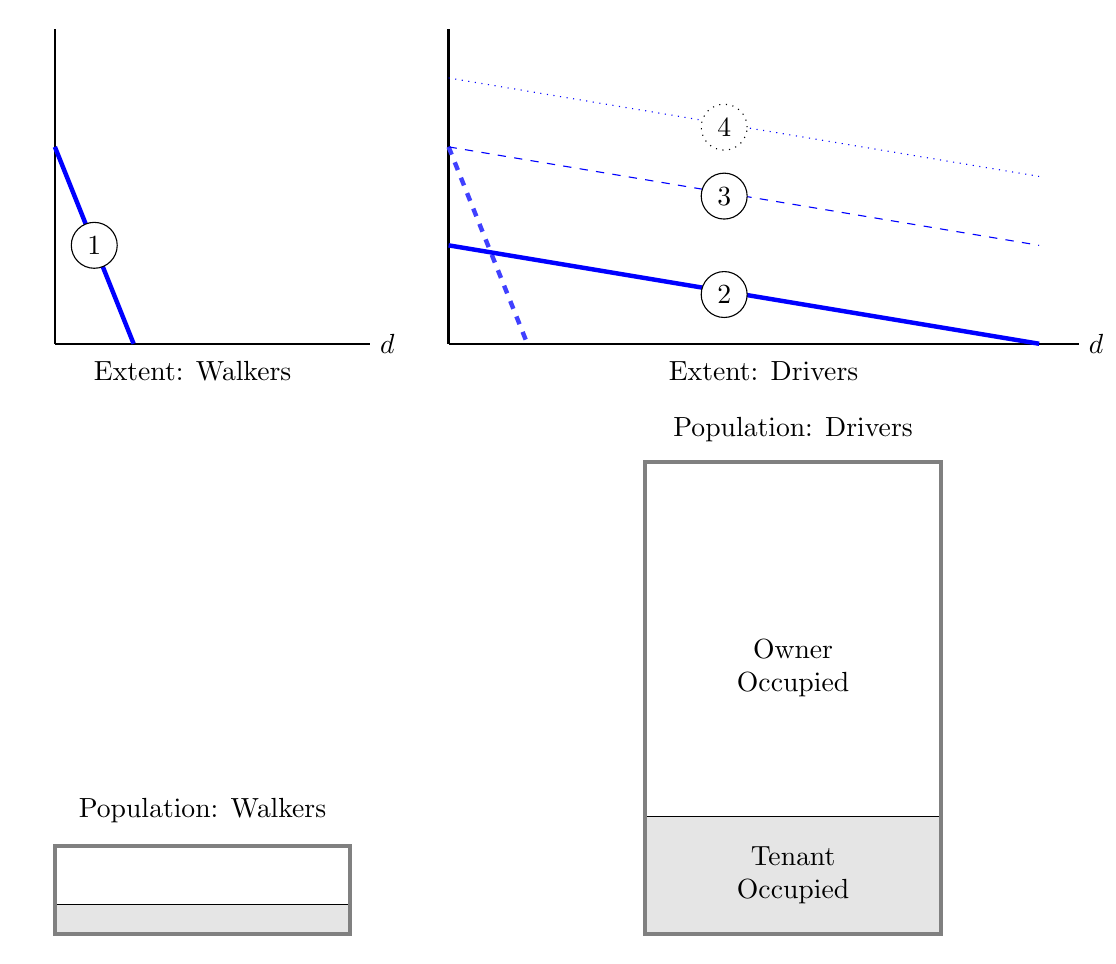
\begin{tikzpicture}[scale=.5]
% EXTENT  BEFORE
\draw[thick](0,0)--(0,8); %Y
\draw[thick](0,0)--(8,0)node[right]{$d$};
\node at (3.5,-.7){Extent: Walkers};
\draw[ultra thick, blue](0,5)--(2,0); 
\node[circle,draw=black, fill=white, inner sep=3pt,minimum size=10pt] (b) at (1,2.5) {1};

% POPULATION BEFORE
\begin{scope}[shift={(0, -15cm)},scale=1.5]%population
\draw [fill=gray!20,] (0,0) rectangle (5,.5); 
\draw[line width= .5mm, black!50] (0,0) rectangle (5,1.5);
\node at (2.5,2.1){Population: Walkers};
\end{scope}

% EXTENT AFTER
\begin{scope}[shift={(10cm, 0)}]
\draw[thick](0,0)--(0,8); %Y
\draw[thick](0,0)--(16,0)node[right]{$d$}; %X
\node at (8,-.7){Extent: Drivers};
\draw[ultra thick, blue!75, dashed](0,5)--(2,0);
\draw[ultra thick, blue](0,2.5)--(15,0);

\node[circle,draw=black, fill=white, inner sep=3pt,minimum size=10pt] (b) at (7,1.25) {2};

\draw[ blue, dashed](0,5)--(15,2.5);
\node[circle,draw=black, fill=white, inner sep=3pt,minimum size=10pt] (b) at (7,3.75) {3};

\draw[ blue, dotted](0,6.75)--(15,4.25);
\node[circle,draw=black, dotted,fill=white, inner sep=3pt,minimum size=10pt] (b) at (7,5.5) {4};
\end{scope}

% POPULATION AFTER
\begin{scope}[shift={(15, -15cm)},scale=1.5]%population
\draw [fill=gray!20,] (0,0) rectangle (5,2); 
\draw[line width= .5mm, black!50] (0,0) rectangle (5,8);
\node at (2.5,8.55){Population: Drivers};
\node at (2.5,4.5)
    [text width=2.4cm, align=center]
    {\baselineskip=20pt Owner Occupied};
%\node at (2,3.3)    [text width=2.4cm]    {\baselineskip=20pt Mortgaged};
\node at (2.5,1)
    [text width=2.4cm, align=center]
    {\baselineskip=20pt Tenant Occupied};
\end{scope}
\label{fig-rent-driving}
\end{tikzpicture}
\caption{Housing tenure post transportation revolution.}
\label{fig-transport-tenure}
\end{figure} 
 
%\input{fig_TransportCost.tex}

The transportation cost revolution brought about by the first street cars and later automobiles made much larger cities possible.  The average walking pace is 2.5 to 4 mph, and new transportation technologies raise this rate by a factor of between five and ten, increasing potential urban area by between twenty-five and one hundred times. 




% THIS IS INTERSTING K.  morgages: Effect of a finbancial instument on urban form!!  suburban flight, second half of the century

%Electric trolleys drew upon manufacturing technology that appeared only in the eighteen eighties and at first only in America. 

%As with other transportation revolutions, institutional as well as technological revolutions were necessary for the interurban phenomenon to succeed.  One such institutional revolution was the creation of the home mortgage in the eighteen eighties.  Another was the development of the public utility, a regulated monopoly, in the earlier twentieth. century.\footnote{https://faculty.washington.edu/jbs/itrans/charge20.htm} The automotive revolution was as important in its way as the coming of the railroads.

%The automobile in time established even more powerful synergies, but they weren't present at the beginning.  Roads suitable for automobiles scarcely existed though new methods of paving utilizing macadam or concrete had recently been invented.  Furthermore, there was no good model in place for road construction.   Unlike the case with either light or heavy rail systems, the vehicles and the road itself were not part of the same corporate entity.       

%Once automotive ownership assumed certain proportions toward the close of the teens of the century, the automobile began to transform the landscape of America in an even more fundamental way than the streetcars had. 

%From the second decade of the twentieth century, the automobile in America has been linked with suburban flight, and when the growth of suburbs reached a crescendo early in the second half of the century, automobile ownership became the norm. 

% Because exurbs are already numerous and growing more so, they place considerable pressure on the Body Politic to ensure that fuel prices remain low, for if prices rise beyond a certain point the exurbanites will be forced to sell out, probably at ruinously low returns because few will choose to live in isolated areas without affordable transportation.  True, exurbs could conceivably be served by public transportation, but only at enormous cost per rider because the population densities are so low in the areas where they are located \dots

% That places the vast suburb dwelling public at risk and the exurbanites most of all.

Initially, rents fell at the centre and rose outside of the original city limits. Lower rents and cheaper suburban housing attract more workers, so that central rents and the land values they support  rise to the original levels and then, because the rising population makes the
city more productive, beyond the original level. 

It  also affected social structure and left indelible marks on the form of cities developing at the time and after. In North America, with large amounts of land, it generated massive urban sprawl, but also made land available for a growing `middle class' of homeowners. This homeowning middle class became the dominant social formation in North 
American society. 

Ultimately the urban expansion generated congestion and rising transportation cost that began to limit urban growth, put upward pressure on  housing costs including transportation, and therefore downward pressure on middle-class effective incomes. Rising congestion costs steepen the rent profile and  reduce the net productivity of cities. Although the process is not a focus of this thesis it represents a relatively simple extension for later work.

\subsection{Differential transportation costs}
 Urbanists agree that before the railroad and the automobile, the extent of a city was roughly determined by how far a person could walk in about an hour. The time and effort cost of transportation determined the size of cities. 
 
 It also affected the distribution of the classes within the city. When everyone walked, the  wealthy may have valued their time more than the poor. In terms of the model, the willingness to pay of the rich would higher  near the core than  the willingness (or ability) to pay of  the poor, but would descend more rapidly with distance
\begin{figure}
\begin{center}
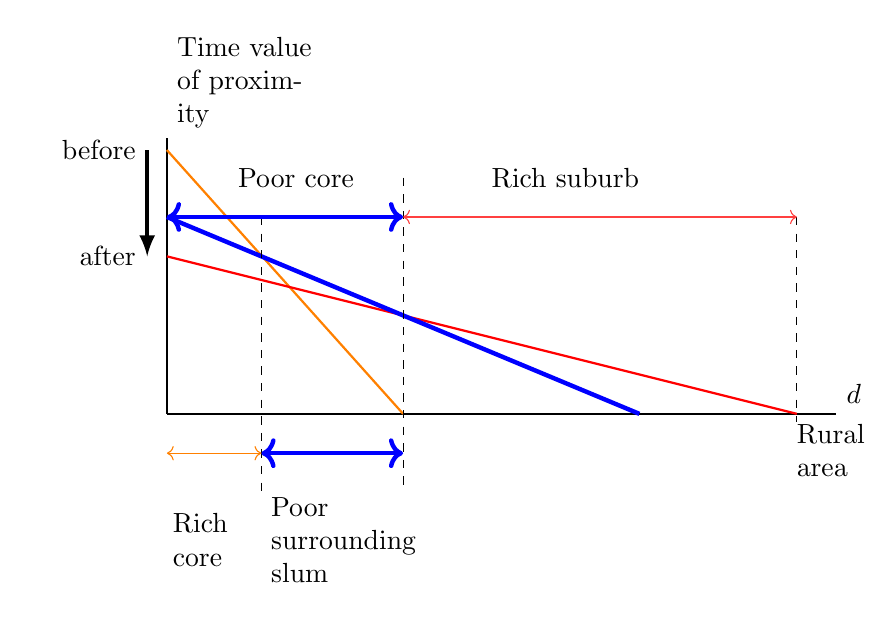
\begin{tikzpicture}[scale=1]
% AXES
\draw[thick](0,0)--(0,3.5)node[above right, text width=1.8cm]{Time  value of proximity}; %Y++
\draw[thick](0,0)--(8.5,0)node[above right]{$d$}node[below, text width =1cm]{Rural area}; 
% BIDS-RENT CURVES
\draw[thick, orange](0,3.35)--(3,0);
\draw[thick, red](0,2)--(8,0);
\draw[ultra thick, blue](0,2.5)--(6,0);

\draw[-latex, ultra thick](-.25,3.35)node[left]{before}--(-.25,2)node[left]{after};
% ZONE DIVISIONS VERTICAL LINES
\draw[dashed](1.2,2.5)--(1.2,-1) ;
\draw[dashed](3,3)--(3,-1) ;
\node at (4,3)[right]{Rich suburb};
\node at (2.5,3)[left]{Poor core};
\draw[dashed](8,2.5)--(8,-.1) ;
%  ARROWS BEFORE
\draw[<->, orange](0,-.5)--(1.2,-.5);
\draw[<->, blue, ultra thick](3,-.5)--(1.2,-.5);
\node[text width =1cm,  left] at (1.2,-1.6){Rich core };
\node[text width =1cm, right] at (1.2,-1.6){Poor \\ surrounding slum};
%  ARROWS AFTER
\draw[<->, blue, ultra thick](0,2.5)--(3,2.5);
\draw[<->, red!75](3,2.5)--(8,2.5);

% \draw[ blue, dashed](0,5)--(15,2.5);
% \node[circle,draw=black, fill=white, inner sep=3pt,minimum size=10pt] (b) at (7,3.75) {3};

% \draw[ blue, dotted](0,6.75)--(15,4.25);
% \node[circle,draw=black, dotted,fill=white, inner sep=3pt,minimum size=10pt] (b) at (7,5.5) {4};
\end{tikzpicture}\end{center}
\caption{A prediction of the basic model: if transportation cost for the rich falls, shifting the orange  bid-rent curve for the rich to the location of the red line, we will see a shift of housing for the rich  from the core to the suburb.}
% \label{fig_fix_my_label}
\end{figure}

 If the technology suddenly provides the rich with commuter trains or automobiles and more attractive sites at the edge of the city, the orange line could drop enough  and become much flatter leading in a flight of the rich to the suburbs, as appears to have happened in many American cities. Lower transportation costs make cheaper land on the edge of the city attractive. This would  offer  more space and the opportunity to build larger homes, a pattern that has emerged in some cities.

\textbf{Experiments}: We first turn off financial  demand and partition the population by wealth and transportation cost to  verify that the predictions made by researchers hold in our model. We then turn financial demand back on  and see if the rate or degree of financialization differs from the base model


\subsection{Municipal costs and revenue}

\begin{figure}
\begin{center}
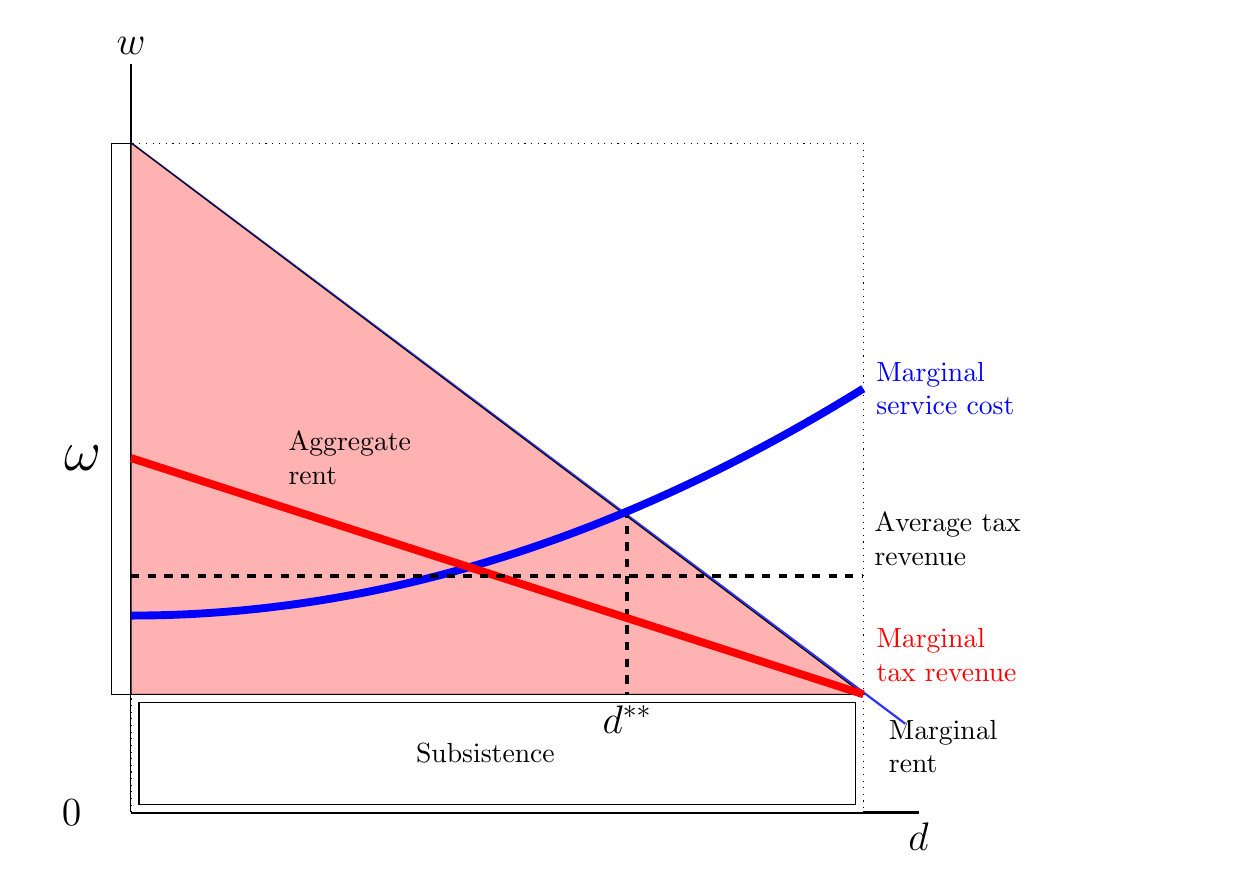
\begin{tikzpicture}[scale=1]
\def\bndmax{5}        %https://tex.stackexchange.com/questions/68462/filling-a-complex-region-with-tikz
\def\bndmin{0.2}
\def \n {8}  % height of y axis
\def \d {10}  % length  of x axis
\def \t {.75}  %  cost of transportation per unit x
\def \th {1}   %
\def \w {7}    %  wage premium
\def \om{1.5}%  omega =rural wage Zero for urban population
\def \azero{2}
\def \aprime {-.0}	
\tikzset{func/.style={thick,color=blue!80}}	
\draw [thick] (0,-\om) --(\d,-\om)node[below]{\Large $d$};  			% Zero for rural population
\draw [thick] (0,-\om)node[left=.5]{\Large $0$} --(0,\n)node[above]{\Large $w$};	% Y axis

%\draw [thick] (0,0)node[left=.5]{ subsistance}--(\d,0);
\node[left=.25] at (0,3){\huge $\omega$};
%\node[left=.25] at (0,\w+.3){subsistence plus};
%\node[left=.25] at (0,\w-.4){wage premium};	

\draw[fill=white, white] (0.1,-0.1) rectangle (14,-\om+.1);
\draw [] (-.25, 0) rectangle(.25, \w);%fill=green!30!blue!30
\node[right] at  (.25, \w/2){Added Productivity};
%\draw [ thick, ->](11.3,-\om/2)--(13, -\om/2)node [right] {\Large $d$};
\draw[fill=blue!40] (0.1,-0.1) rectangle (9.2,-\om+.1);

\draw[fill=black!0, dotted] (0,-\om) rectangle (9.30,\w);% new product repeat
\draw[func, domain=0:\w/\t+.5] plot [samples=200] (\x,{\w-\t*\x}); %rent profile
\draw[fill=blue!0] (0.1,-0.1) rectangle (9.2,-\om+.1);
\node at (4.5,-\om/2){Subsistence};
\draw[fill=red!30,] (0.,0.)--(0,7)--(9.30,0.)--cycle;% Rent \w-.2
\node[text width=2cm] at (3.,3){Aggregate \\rent}; 		%Rent 
%\node at (5.8,5.7)[]{\Large Transportation};
\node at (6.3,4.8)[white]{\Large expenditure};
\draw[ line width=.5mm, dashed] (6.3,2.35)--(6.3,0)node[below ]{\Large $d^{**}$};

\draw[func, domain=0:9.3, line width=1mm,blue, text width=2cm] plot [samples=200] (\x,{1+\x^2/30})node[right]{Marginal\\ service cost};
\draw[ line width=1mm, red] (0,3)--(9.3,0)node[above right, text width=3cm ]{Marginal\\tax revenue};
\node at (9.5, -.2)[below right, text width=2cm]{Marginal rent};

\draw[ line width=.5mm, dashed] (0,1.5)--(9.3,1.5)node[above right, text width=2.5cm ]{Average tax revenue};
%GRID
%\draw[step=1cm,gray,very thin] (0,0) grid (10,10);
\end{tikzpicture}
\end{center}
\caption[The Alonso model with municipal costs and revenue.]{The Alonso model \gls{rent profile}, as illustrated in Figure~\ref{fig-alonso-simple}, with cost and municipal costs and revenue added.} %service fees added.}
\label{fig-municipal-costs}
\end{figure}
 

 Two stylized facts should be noticed. The first is that the marginal cost of servicing generally rises with the distance from the centre. Figure illustrates the general form of servicing costs, but not the relative scales of rent and servicing costs. When this observation is combined with the \gls{Henry George Theorem} the conclusion is that the optimal size of the city  is at  $d^{**}$, where marginal service cost intersects with the marginal increase in total urban rent.  Walter Christaller, 1933

The second stylized fact is that property taxes, which are generally  fixed as a share of property value, decline as the distance from the centre increases. Figure~\ref{fig-municipal-costs} illustrates the general form of tax liabilities, although it does not  accurately represent their relationship to rent or  servicing costs. This implies that in many or most urban situations the residents at the outer edges pay less than the average amount in property tax per unit of land, but cost  the community budget more than the average amount. In essence, the central city subsidizes the suburbs. (see Perverse Cities \ref{blaisPerverseCitiesHidden2011}). This arrangement is both economically inefficient and unfair, but it has been built into the fiscal structure of cities largely as a result of automobile-based urban growth. It is likely that this fiscal misallocation saps some of the potential productivity growth of cities. Property taxation reduces the market value of properties, but it also funds services and amenities that increase the value of properties. 

Both servicing and taxation effects are more variable and than the simple model suggests.  One conclusion urban theorists draw based on variants of the Alonso model is that because property owners in the low-density urban margin are subsidized,  the subsidy is likely to create serious fiscal problems for municipalities in the long-term and result in serious inefficiency in land use.

Political opposition is essentially rent seeking.

}
\chapter{Conclusion} \label{chapter-conclusions}

MAYBE SOMETHING LIKE THIS IDEA FROM ABSTRACT? Cities are at the heart of how people create value, there's a gap, however, in the formal apparatus in standard economic theory for analyzing the distribution of the enormous value created in cities.


The dissertation examines the hypothesis that financialization induces a shift towards tenancy among the urban workforce. We then explore the possibility that redirecting spatial rents results in decreased urban productivity. 
It brings together \gls{neoclassical growth theory} and recent empirical and theoretical work on \gls{urban scaling} to build a model of an urban system to explore financialization in the context of housing markets and we explored the systemic effects of the shifting ownership of property in cities on the distribution of wealth and the potential that this shift can actually change the ability of cities to grow, thrive, and produce wealth.


Financialization of the housing market is a flow of money into the housing market but not in to housing production, expanding financial ownership and tenancy, while reducing the share of owner-occupied housing. Its goal is the capture of spatial rents, which we will show has implications for both the productivity and the class structure of the city. 
In the urban context, financialization is fundamentally \gls{rent-seeking}, and we show it can have a profound impact on the system, including effects on both distribution and productivity. 

A key insight is that the financialization of the housing sector is a form of \gls{rent-seeking} that must have detrimental effects on urban development and on the well-being of urban residents, that is neither constructive nor productive.

WHAT ARE THE 6 POLICY EXPERIMENTS

% We built a model that brought these togterh SUMMARIZE...Based on .... REVIEW TEHORETICAL BASIS FOR HYPOTHESIS... we hypothesized WHAT
SUMMARIZE CONCLUSIONS.... AS EXPECTED AND WhAT WAS SURPRISING>...
There are two classes of results first on ownership, the second on productivity. ADD DETAIL

THIS WORK LAYS THE GROUND WORK FOR FUTURE STUDY OF ....

% The analysis suggests that in addition to the recognized distributional consequences, the housing crisis has productivity impacts that should be considered in developing urban and housing policy. 

We argue financialization %This dissertation makes the case that it
has worrying implications for the success of cities and the nature of our social fabric. 
The housing crisis raises the question of whether Canadian cities can continue to attract people and accumulate wealth for its residents and industries, and whether they can sustain their growth.


\section{Consider}
OR *** ADD BACK? any of this


sketches how this thesis relates to four major fields: classical rent theory, neoclassical production theory and growth theory, the scaling literature, and urban spatial models. % \dots , and the role of space as a unifying factor across three of the fields. % WITH FINANCE IS SPACELESS.
    This work draws together sub-literatures including rent theory, production functions, the standard urban model, growth theory, urban growth theories, financialization, and the theory of distribution, so the chapters review those areas. % *** link the areas to the chapters better?  %theory for our analysis, 

    , using an approach similar to that developed in modern growth theory, that we discuss in Chapter~\ref{chapter-rent}.  In that chapter we ground the observation in  \gls{neoclassical growth theory} and recent empirical and theoretical work on \gls{urban scaling}. 
 We take a step beyond integrating labour markets in a city, to studying the distributional effects: who gets the surplus, what does that mean for the class structure, and ultimately the productivity of cities. 
We began with the fact that there is growing policy concern about the financialization of  housing. We have produced 


\section{OTHER PIECES TO CONSIDER ADDING}

 % We take a step beyond integrating labour markets in a city, to studying the distributional effects: who gets the surplus, what does that mean for the class structure, and ultimately the productivity of cities. 
% We began with the fact that there is growing policy concern about the financialization of  housing. We have produced 

% In this thesis we began with the broad question of how urbanization and financialization interact. To explore this question, 


% THINGS TO INCLUDE


% VS  This work draws together sub-literatures including rent theory, production functions, the standard urban model, growth theory, urban growth theories, financialization, and the theory of distribution. % , so the chapters review those areas. % *** link the areas to the chapters better?  %theory for our analysis, 

    % , using an approach similar to that developed in modern growth theory, that we discuss in Chapter~\ref{chapter-rent}.  In that chapter

 % THIS WORK DRAWS TOGETHER - THEORETICAL FRAMEWORKS....We sketch sketch how this thesis relates to four major fields: classical rent theory, neoclassical production theory and growth theory, the scaling literature, and urban spatial models. % 
 % TODO add backThe organizing principle in the spatial models of all three disciplines is an economic variable, land rent.  The three disciplines share a simple economic insight.  ADD LINK and the role of space as a unifying factor across three of the fields. Past work did not  bring together spatial insights with production insights in this way.... Because its a economic and urban question FIX  -- WITH FINANCE IS SPACELESS.

% We have used what we call the  \textbf{\gls{Alonso-Jacobs model}} to explore the source and distribution surplus value. We  work with an extension of the basic Alonso model that incorporates the \glspl{agglomeration effect} that Jane Jacobs  described in her book, The Economy of Cities \cite{jacobsEconomyCities1969}. In our model these effects generate the \gls{urban wage premium} central to urban growth. % and the wage premium. 

% The result is a simple model in which marginal productivity determines the wage, the wage determines the size of the city, the size of the city determines the labour supply, and labour supply determines marginal productivity. 

% The economics is clear that this is what's at stake is productivity of cities, the distributive features of the economy and the impact of the middle class. 
% Highlights the urgent need for more empirical work.


% Particularly, it centers concern with implication for urban development of growing rent extraction by the financial sector. 
% Our focus is land rents, %but in the context of an urban economy. 


% This appears, at least part of it appears as locational rents. 
% Financialization, is about capturing the surplus generated by the city.  % To model the financialization of land markets.

% To model financialization we need rent because
% To develop a formal model of financialized urban land markets, we introduce rent because rent is % precisely   about extracting and allocating surplus value in a system. % and that is what financialization of the housing market is about/does. 
% The classical approach to rent is a core tool in the development because it brings the extraction of surplus into focus.
% GAP Nobody has linked the rents - linking rents to urban scaling. Beteencourt is talkign about a surplus in the system, wealth, but he hasn't linked to the market/land market for those locational rents.


% - hamstrings the whole thing.
% --> the whole system as a welfare producing system fails if the value gets sucked out---CONCLUSION TH THESIS---fails from a social point of view-
% these are averages---some are structurally below average so some are always behind simply because of the structure of the rents claimed.. that's built in FUTURE WORK- DIFFERENT INCOMES GETS YOU THAT. 


% We could run off a cliff and accidentally destroy the middle class, we should consider the implications, need a language to explore that.
% ---


% We examine the effect of housing on wealth inequality by looking at 

% Adding 2 things 1. rent extraction and 2. power law scaling of productivity, we find rent is the breaks on the engine of wealth creation

% If the links are correct. 



% There is a market for the urban product produced by firms, and a financial market that agents can invest in.

% ---


% WAS AT END OF SPACE CHAPTER 
EXPLAIN THE CONTRIBUTION MORE CLEARLY
Other theories of space and transportation costs  don't examine distribution or how the distribution of rents might affect the productivity of the city, which means they throw no light on the effects of the financialization of the property market on distribution or on urban productivity.  This is the limitation we seek to address in this thesis. 

We build the  standard urban model into our model of financialization by using the concept of rent as it appears in the urban system


We explore distributional consequences, how the distribution of rents feeds back into the productivity of cities, and how the urban economy is changed by the financialization of urban housing. % and relating them to neoclassical growth theory.  
% % This chapter introduces the background to the theory of the urban model. 
% E ADDED: 
By combining these pieces we can look at how ownership changes with finalization, how that can feedback into changing the process of value creation in the urban center.
% Rent provides a  neglected indicator or state variable in the urban system. It can be  seen as an indicator of the state of teh system that has been largely neglected.





----

% The 3 parts of this do xyz
% The dissertation is organized into three parts: background, methodology, and analysis. The background section provides theoretical foundations and reviews relevant literature, while the methodology section outlines the model framework. The analysis section presents results from simulations and discusses their implications.






% We have a model of productivity to change. 
%\textbf{We are in a housing crisis.  These are things that can illuminate this particular.. **}
We examine how urbanization and financialization interact through urban housing markets. %The dissertation examines a pair of linked hypotheses about the evolution of an urban system: firstly, 
% ## Contributions:

%To test the 
%We built an agent based model to explain tenatization.
% models for each class of agent in the system and then allow agents to interact. 
% Firms hire workers if it is profitable. Firm productivity and wages rise with population due to agglomeration effects. 

% Rural workers near the city apply for urban jobs if the urban wage justifies travelling to the city center to work. Homes come up for sale when workers retire New entrants buy homes if they can afford homes, otherwise they become tenants. Investors purchase or sell properties if the net rent and capital gains exceed the return on alternative investments. % this paragraph describes an agent-based approach and establishes the independence of the agents 

%They don't live in the city, they can't reinvest, they don't belong to the class of those who own property and can save through homeownership. 

 %in a %spatially explicit urban land market. 
The most complex part of the model is the financial bidding for property by different agents. Firm technology and the price of output are held constant. Investors represent the supply of global capita and are by assumption non-resident.

It also allows us to see how the locational rents generated by the city is distributed between investors or residents.  % This paragraph says that results emerge from the interaction of independent agents./
 % is captured through land rents. 
By capturing rents, financialized actors are able to capture a share of urban productivity.  
In the model, this affected the systemic effects of the shifting ownership of property in cities on the distribution of wealth and the potential that this shift can actually change the ability of cities to grow, thrive, and produce wealth. 
% Big chunks simplified but the guts are in financial behaviour. 

% It is helpful for economic policy in complex environment. 
The model allows us to test qualitative effects of various policies.



%----------------------------------------------------------------------
% END MATERIAL
% Bibliography, Appendices, Index, etc.
%----------------------------------------------------------------------

% Bibliography

% The following statement selects the style to use for references.  
% It controls the sort order of the entries in the bibliography and also the formatting for the in-text labels.
\bibliographystyle{plain}
% This specifies the location of the file containing the bibliographic information.  
% It assumes you're using BibTeX to manage your references (if not, why not?).
\cleardoublepage % This is needed if the "book" document class is used, to place the anchor in the correct page, because the bibliography will start on its own page.
% Use \clearpage instead if the document class uses the "oneside" argument
\phantomsection  % With hyperref package, enables hyperlinking from the table of contents to bibliography             
% The following statement causes the title "References" to be used for the bibliography section:
\renewcommand*{\bibname}{References}

% Add the References to the Table of Contents
\addcontentsline{toc}{chapter}{\textbf{References}}

\bibliography{thesis-bib.bib}
% \bibliography{bib_resilience,bib_housing}

% Tip: You can create multiple .bib files to organize your references. 
% Just list them all in the \bibliogaphy command, separated by commas (no spaces).

% The following statement causes the specified references to be added to the bibliography even if they were not cited in the text. 
% The asterisk is a wildcard that causes all entries in the bibliographic database to be included (optional).
% \nocite{*}
%----------------------------------------------------------------------

% Appendices

% The \appendix statement indicates the beginning of the appendices.
\appendix
% Add an un-numbered title page before the appendices and a line in the Table of Contents
\chapter*{APPENDICES}
\addcontentsline{toc}{chapter}{APPENDICES}
% Appendices are just more chapters, with different labeling (letters instead of numbers).
% % Main
% \chapter[Future Work]{Future Work}
\label{appendix-future-work}



In  this chapter, we discuss potential extensions of our basic model.  Models are by nature combinatoric: every added element involves making a choice among alternative assumptions and implementations. A model incorporating in binary choices is one of an implicit family of $2^n$ alternative models. We have sharply restricted our model  in order to focus on one process of significance, financialization.  This is in part so that we can explain and justify each assumption that we use, and in part because only sharply restricted models produce understandable results. 
% Those results are condition on the specific set of assumptions to ensure that 
We have designed the model to  accommodate a range of extensions that are either theoretically or interesting or important for policy-makers. 



Figure~\ref{fig-logic-extensions} illustrates  five general types of extension. The first is to move from a static population to a model with population pressure. This appears on the left as a group of three new subroutines with connections to the elements of the model most directly affected. Some links are left out to keep the figure readable. Examples of omitted links  are the channels through which  population affects labour supply and savings.  


A second class of extension would introduce a housing production sector. This appears on the right side of of the figure linked to the banking sector. It requires adding a dynamic housing  stock. 

A third major class of extensions, separable from production is to introduce variation of housing form,  density and amenity. Zoning restrictions and building codes are related. Many questions about who gets what housing arise at this point. 

{\newpage\thispagestyle{empty}
\vspace{-1.5cm}
\begin{figure}
\vspace{-4.5cm}
\begin{adjustwidth}{-0.24\textwidth}{-0.2\textwidth}
\centering
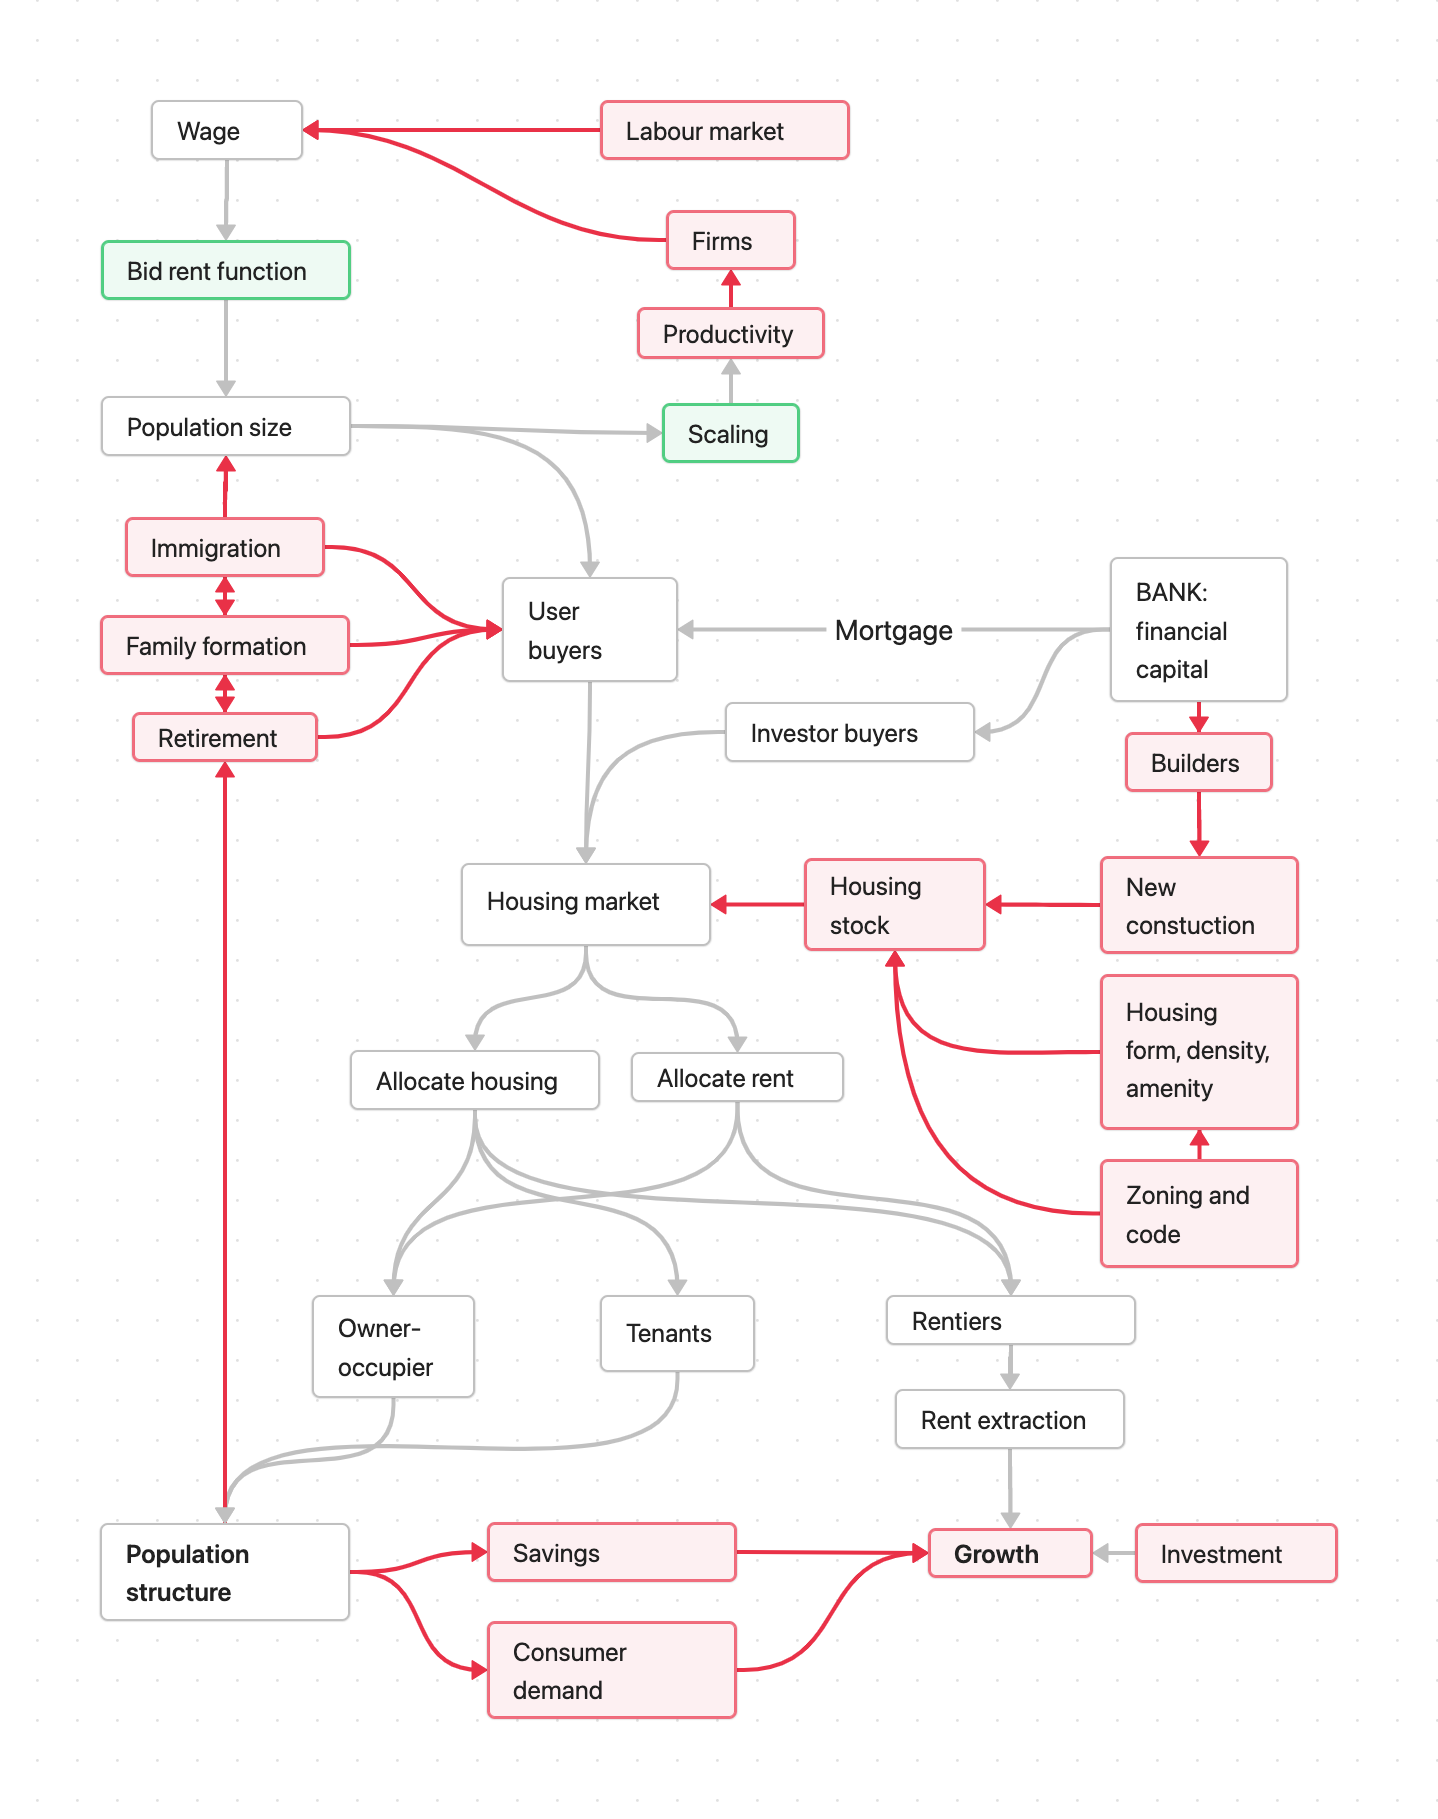
\includegraphics[scale=.22]{fig/extensions.png}
\end{adjustwidth}
\caption{Extensions}
\label{fig-logic-extensions}
%\pagestyle{headings}
% \usetikzlibrary{positioning}
%\begin{tikzpicture}[remember picture,overlay,shift={(current page.north east)}] \node[anchor=north east,xshift=-1cm,yshift=-1cm]{\includegraphics[width=1cm]{example-image-a}};\end{tikzpicture}

\end{figure}
}


At the bottom of the figure we introduce consumer demand linked to the population structure and feeding back to growth. Savings behaviour becomes more  complex when consumer demand is made endogenous and with as more complex population structure.

The fifth block of extensions illustrated in Figure~\ref{fig-logic-extensions} would replace the simple, scaling-based transmission mechanism in the Alonzo-Jacobs cycle with explicit firm and labour market behaviour. This class of extensions is obviously linked to population structure. It leads to consideration of firms that produce different products, some for export some for the local market, and to multiple types of labour.

Linked to the labour market and production system is the possibility of introducing competing cities. 

It should be clear that each of the extensions we suggest is potentially as complex as our core model, and each brings with it a collection of additional assumptions. We would argue that none of them would change our qualitative results greatly, although each would deepen our understanding of mechanisms and of the detailed impacts.


\section{Population pressure } 
Our basic model does not have a growing population. This conveniently allows us to isolate certain effects of financialization. Population pressure is one of the drivers of financialization because it amplifies speculative gains, however. As a result, one of the first extensions must be  to introduce population pressure.

There are two sources to consider: 
\begin{enumerate}
\item agglomeration effects that increase the wage and attract workers faster than the housing stock can respond. 

Worker agents from outside the city can always consider moving and accepting a job. 
% QUESTION - how to manage the flow of new agents?
%, or can make more from rents and moving away
\item immigration pressure
\end{enumerate}
under the  first, agglomeration economies drive population while under the second, population growth may drive agglomeration.

The growth of the housing stock will generally lag population growth, generating price effects and stock dynamics.

Agents will respond to increases in demand conditions. The perception that the market is tight or that prices are rising may lead to higher bids and reservation prices and shift results in favour of sellers.  


%Buyers could consider neighbourhood pressures, demographic changes, changes in job location, desire for amenity etc. in their assessment of housing need. 

%With multiple bids agents can place the most competitive bids on those homes they prefer. If they have higher urgency they place strong bids on more homes. 

%Next buyers request a selection of homes to consider from a real estate agent. Those with higher need for housing look at more homes. The real estate agent offers a selection of homes based on the agent's requirements. A randomness parameter determines how many divergent houses are also considered. When the parameter is 1, the selection of homes is fully randomized, When it is 0, the agent sorts all available homes and offers those which fit the agents budget, space, and other requirements best.


\subsection{Retirement investors and private investment properties}
The simple population turnover in our model can be replaced with a more complex set of possibilities at the agent level.  At retirement,  agents can be allowed to may choose between selling their home, renting it as an income property, or if there is sufficient amenity value for them, staying in the city. Implementing these choices complicates the agent decision and the resulting housing distribution but require few changes to the rest of the model.

\section{Housing production}

\section{Differences in density, housing form, and neighbourhood amenity}
Much of what is interesting in a city is the rich variety of housing forms and neighbourhoods and the varied populations that occupy them. Our model has a single form of housing and an undifferentiated populations, allowing us to differentiate the housing system in specific ways and study the interactions between the built world and the population. We are convinced that few of the possible extensions could affect our qualitative results. 

Nonetheless, in our agent based model, in which every lot is  addressable, it is simple to introduce zoning boundaries, local amenities, different densities or housing qualities and homes of different sizes. Hundreds of experiments are possible exploiting  the extensibility we have carefully conserved.  

We can ask what would be the effect of a hard zoning boundary and what would be the effect of suddenly relaxing it. We could explore the effect of speeding the rate of conversions from one size  home to another, or of locating high density pocket on a transportation route. Many significant urban policy questions could be examined with a limited amount of additional programming. 

\section{The consumer city}
Much of the demand for what is produced in the city is local consumer demand.  Our model has assumed there is production only for a perfectly elastic export demand. Consumer needs are buried in the subsistence wage. 

A minimal extension would be to introduce a second sector representing local consumption demand. A share of locally generated income would support production for the city's population. The labour force would be split between the two sectors and both productivity and wages might differ across sectors. 

A more complex treatment would introduce a range of service, entertainment and retail producers. This might be done monopolistically competitive firms \'a la Dixit and Stiglitz \cite{AvinashK.Dixit1977MCaO}.



\subsection{Distribution of rents}
Rents go to landowners, with a share taken for maintenance and taxes.
Rents may also be taxed, could be shared between multiple owners, etc.
 %\note{REPHRASE? rent is  extracted from the coalition of capital and workers.} % Rents may also be taxed, could be shared between multiple owners, etc. 
%The rents are captured by landowners.  The capture of rents by landowners is common buy not necessary. 
In principle the gains from urban productivity and amenity can be allocated as social wealth through shared ownership, as is often done on a small scale with cooperatives and land trusts, distributed to all citizens through something like a social wealth fund, or captured in taxes or fees as Henry George suggested. 
%The rents would otherwise go to labour and capital.





\subsection{Urban Savings - Contributions?}
THIS IS A CONTRIBUTION, BUT ALSO A DISCUSSION OF ONE WAY THIS WORK COULD BE EXTENDED, MIXED WITH A BIT OF MODEL DESCRIPTION

Conventional growth models specify a savings/investment mechanism at the national level. To our knowledge, this has not been done for the city level. We require  savings at two levels. First, since we want to incorporate  households home ownership and a relationship to the financial sector through mortgages, We specify a savings rate out of the spending we have isolated in the `subsistence wage' This means that both urban and rural workers accumulate savings, that savings are age-dependent, making the size of mortgage available also age dependent. 

Homeowners in addition have equity $E=P-M$ in their homes.  ({\color{red}Should newcomers also have equity? or is it built into the savings. Clarify this.} 

A second level of saving is the  investment in capital out of the city surplus. Even raising this question puts us into terra incognita. There are many  channels through which surplus flows into productive investment in the urban contest. One is through public investment in infrastructure. We have discussed how falling transportation costs increase surplus generation. Investments like this are made slowly and take effect over time periods much longer than our model is concerned with.  We can set a property tax rate   that we will assume is sufficient to maintain the stock of infrastructure.

Public and private investment in human capital is largely urban as well, but as with infrastructure, investment and response take effect over time periods much longer than our model is concerned with. 

Private sector innovation in technology, marketing, or products draws on local saving less but still significantly on local savings. We have little in the way of theory or empirical research on this channel. Lags between investment and any rise in the urban wage premium are almost certainly long and variable. 

We deal with this issue by linking local capital ownership with the scale factor. It is known that local ownership is associated with local investment. We will assume that local capital ownership, which consists in part of local ownership of the housing stock, can be proxied by homeowner equity as a share of local. 

\subsubsection{savings and retirement behaviour}
Agents fund their retirement from savings, as well as returns on their home if they have one to sell. Savings may be invested in a pension fund, or in local property,  depending on expected risks and returns. In the real world, financial institution manages most pensions, investing in the market or in property.  All this institutional structure is probably most easily handled by implementing a savings account for each agent. We are not interested in the detailed investment behavour for the financial sector.% either in the stock market, or in pensions.

%Institutional and individual investors can access debt. %

We could also consider a case where outside money can come under institutional management, not just local retirement savings. A parameter would control the inflow of additional money beyond local investment in the pension fund. 



\section{Making  labour market and firm behaviour explicit }
We have carefully developed the link between neoclassical growth theory and the literature on urban scaling \cite{bettencourtIntroductionUrbanScience2021} and  We then imposed the scaling result on our model.  We force the model to conform to the empirical data on the relationship between population and productivity. This amounts to black-boxing the entire production and labour demand sector as well as the construction and housing production sector. 

This made sense because our focus  was on the housing market and the financial sector, but the model we have constructed will allow us to ``fill the black box'' with more complete models of the production and labour market to see how they compare to the empirical data. 

The  scaling  literature also provides relationships between density and population and infrastructure cost and population that we can explore in the same way.

In the scaling literature, these relationships are increasingly theorized in terms of network effects, which is perfectly consistent with the Jacobs analysis and the more recent neoclassical growth modeling.


\subsection{The transmission puzzle}

The transmission of productivity increases arising from agglomeration effects  to the urban wage through firms, can be modelled in many ways. The agglomeration effects are external to the firm and therefore likely to be unexpected. If  firms underestimate the marginal product of labour, labour productivity will be greater than expected, output will be higher than planned output, and revenue and profits will therefore be higher than expected. Excess demand will attract more productive capital which in turn will demand more labour,  Rising labour demand drives up the wage. The agglomeration effect driving growth is essentially a public good in which individual firms will under-invest. This raises a policy challenge that we leave for others. CLARIFY - ALSO STILL A FOOTNOTE IN MODEL SECTION. CUT OR REF THEiR IF MOVING HERE.

 It is straightforward to compute the rate of excess return for  this model. 


\begin{figure}
    \centering
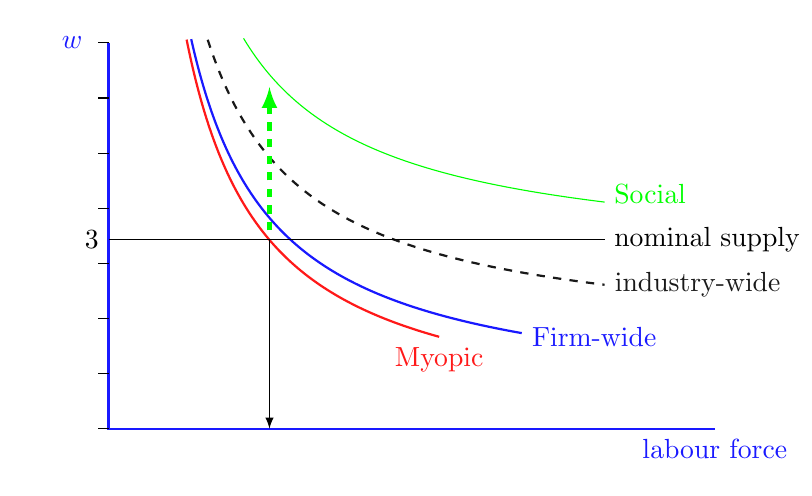
\begin{tikzpicture}[scale=.7]
%\def\bndmax{5}        %https://tex.stackexchange.com/questions/68462/filling-a-complex-region-with-tikz
%\def\bndmin{0.2}
\def \Y {7}  % height of y axis pecent
\def \W {15}  % length  of x axis
\def \Wbar {3} % jmeam wealth
\def \omega {3}
\def \A {1}  %was .5
\def \B {.5}

\draw [thick, color=blue!90] (0,\Y)node[left=.2cm]{$w$} -- (0,0)--(\W-4,0)node[below]{labour force};  
 \foreach \yi in {0,...,\Y} \draw (0,\yi)--(-.2,\yi)node[left]{};
 
\tikzset{func/.style={thick,  color=blue!90}}
% \draw[ func, domain=.2:\W-6] plot [samples=200] (\x, 2*\x^.5)node[below=.1, right]{SUPPLY};

\tikzset{func/.style={  color=green}}	
\draw[func, domain=2.45:\W-6] plot [samples=200] (\x, 10/\x+3)node[above=.1, right]{Social};

\tikzset{func/.style={thick, dashed, color=black!90}}	
\draw[func,domain=1.8:\W-6] plot [samples=200] (\x, 10/\x+1.5)node[ right]{industry-wide };

\tikzset{func/.style={thick, color=blue!90}}	
\draw[func,domain=1.5:\W-7.5] plot [samples=200] (\x, 10/\x+.4)node[below=.05, right]{Firm-wide};

\tikzset{func/.style={thick,color=red!90}}	
\draw[func,domain=8.5/6:\W-9] plot [samples=200] (\x, 10/\x)node[below]{Myopic};

\draw[](0,3.425)node[left]{$\omega$}--(9,3.425)node[right]{nominal supply };
\draw[thin,latex-](2.92,0)--(2.92,3.425); %a vertical labour supply
\draw[ultra thick,dashed, green,-latex](2.92,3.6)--(2.92,6.2);
%\draw [blue,  thick](13, 8.3)--(15,8.3)node [right, black] {\small A=\ 1,\ B=0.5};
%\draw [green, thick](13, 7.6)--(15,7.6)node [right, black] {\small A=.8, B=0.8};

%\node at (5,-1.5){Resulting in  profits, expansion, and/or entry: the city grows};
 \end{tikzpicture}
\caption{Multiple marginal products.}
\label{fig-marginal-products}
\end{figure}



Figure~\ref{fig-marginal-products} illustrates the problem. We can  make a distinction between the myopic marginal productivity curve observed by at the shop floor level and  the firm-wide effect of adding a worker. The red curve labeled ``Myopic'' represents the declining direct marginal productivity of labour as in might be observed by a shop manager, who could report how much more output one with one worker one lathe would produce. The blue line above it labeled ``Firm-wide'' represents the actual effect on firm productivity that arises because the new worker makes other workers in the firm more productive. This addition to output would be observable for managers reviewing the firm's performance over time. ' 

We can go on to consider the slower and distributed effect on closely related firms, which would raise any estimate of marginal product.  If there are 10 other firms and a new worker  has a small spillover effect  $\epsilon$ on each,  the spillovers raise the industry  marginal product  by $10\epsilon$. Each of the  10 other firms  enjoys  an additional $10\epsilon$ gain in the marginal product of their workers. This should lead to additional hiring by other firms.

Finally, expanding our view another step, we notice that if each of the  10 other firms hires one worker who produces an additional  $10\epsilon$ gain in output for all firms, the total spillover effect would rise by $100\epsilon$. The social marginal product of a single hire is indicated by the green line. 



\section{The system of cities}
Modern cities are not lonely and autarkic  beasts wandering their own exclusive territory and unconnected to others of the species. They are one is a global system of cities that compete and complement each other. Information, capital and even labour flows between cities are large. Henderson Abdel-Rahman\cite{Henderson1972Sizes}, Abdel-Rahman \cite{abdel-rahmanAgglomerationEconomiesTypes1990}, Fujita \cite{fujitaMonopolisticCompetitionModel1988}, Fujita, Krugman, and Venables \cite{fujitaSpatialEconomyCities1999}, and Fujita and Thiess \cite{fujitaEconomicsAgglomeration1996} among others provide models for expandingh the model in this direction.



\subsection{Taxes, municipal government, public goods, and productivity,}
This is a major issue with considerable development in the economics literature. Property taxes reduce the net locational value that flows to an individual owner but provides services and wages that make the city attractive. 

(create a regime where particular groups have an advantage)

Localized tax advantages can move a share of financialised investment into private consolidation of land.
including the structure of taxes for investment properties, institutional investors, individuals, etc.




\section{TO  METHODOLOGY?: Distribution}% not the right word
ABMs can be run multiple times to produce distributions of expected outcomes, which makes them valuable in planning exercises. They also do not require that we use a representative agent to make them tractable. Our model is intended to be elaborated  for such use. 

extensions
what it is
why it would be great to model
why it doesn't matter for our core results

\section{A possible typology of models and experiments}
While there  are many variations on the basic urban model and many potential experiments with each model there are only a few of immediate interest if the goal is to text the ``resilience'' of equilibria.

These models may exhibit irreversibilities in variables such as distribution, homelessness, city form, and class structure. 

The basic strategy for examining the system resilience is to shock a model (experiment) and then see if diagnostic variables recover. (This needs more precise expression.)

The first task is to select a subset of models an experiments that are of particular interests with respect to.

The second is to construct a model that allows those case to be examined. Ideally the model would be easily adapted to other experiments.

The following is a an attempt to develop a typology with a clear progressive structure.

Feedback - wealth allows upgrading. This advantages the rich. Maybe this 

\subsection{Models}
\begin{enumerate}
\item \textbf{A: The basic model}

The workhorse of urban economics is the circular city model. Some feature of the central place generates rents. It may be that it is the only employment centre. It may be economies of scale to a single activity or synergies arising from various externalities\footnote{We are interested in agglomeration economies. The wage  structure would then be related to the population or industry  structure. Externalities driving agglomeration may be classified  into two types, the  or so-called ``Marshalian''  and ``Jacobs'' externalities.}. 

In the simplest model, the central place pays a uniform wage, $w$ to all employees, who have identical preferences and transportation costs. $w$ is an attribute of individual residents. Residents  purchase or rent equal quantities of land at differing locations $l$ for identical housing.  

There are transportation costs $T$ that depend on distance from the  central place, so land close to the central place is more attractive than land farther from the central place.  

The equilibrium concept is that a market with identical individuals with identical incomes and transportation costs will result in identical utilities. The result is that land rent must decline with distance from the central place to offset rising transportation cost. 

The size of the city is determined by population and lot size. Income and transportation costs will interact with lot size. The basic model can be initialized by matching the number of properties to the size of the population. 

If population exceeds the number of properties there are three margins to consider
	\begin{enumerate}
		\item The land supply can increase. There may be a conversion cost
		\item The land per-capita may decrease. This is not simple in a city with land-use regulations, zoning, and fixed capital in homes. A conversion process has to be defined
		\item A homeless population can emerge. 
	\end{enumerate}

It is convenient in this model to use a \gls{Cobb-Douglas} utility function that has the property that a fixed fraction of income is spent on housing.  We can start with the assumption that earnings are fixed for the lifetime at the one-period wage, $w$. Then total spending on housing is $\beta Y, \beta <1$ and $ Y=w$. Let the transportation cost for a specific location $l$ be $T(l)$. The  equilibrium price at that location will be $P(l)= \beta Y-T(l)$.

It is convenient but not necessary to assume that land outside of the residential limit is costless. It is common to assume a fixed price for agricultural land. 

There is no fixed boundary and the size of the city is determined by the utility that can be achieved in competing regions of competing

\item \textbf{Y: The basic model with Income Differences}
This will result in segregation by neighbourhood depending on income. 

Income can be purely earning, which requires a distribution of $w$ across agents. Income  might include investment income, which  a private rate of return and a distribution of assets across agents. \footnote{A more subtle model could allow individual wages to be linked to the agglomeration of other workers - say engineers. we can imagine a city that has centres of agglomeration by profession or by complementarity. Depending on the production function, this should emerge endogenously.}
\footnote{Sufficient investment income could lead individuals to locate in cheap properties at the edge of the city.  Income might also be invested in property affecting the quality of a unit. This would require incorporating unit quality in the attribute list for each property, and introducing a quality preference  in the attribute s of residents.}

\item \textbf{L: The basic model with Locational Preferences}
This will result in segregation by neighbourhood depending on preferences.

One version would be include distance to the edge of the city as an amenity in the utility function. Another would be to locate amenities within the city. These would lead to higher prices near amenities.

A natural variant would be to have earning depend on location. If there were several locations  a polycentric city would emerge.

\item \textbf{T: The basic model with varied transportation cost }
This will result in segregation by neighbourhood depending on income and Transportation costs. Experiments include cars for the rich and  transit. 

Diagnostics include change in total transportation cost and differential welfare effects.

\item \textbf{R: The basic model with a rent-own choice}
This may result in the emergence of classes. Agents must have the capacity to borrow to purchase. Attributes of the agents and must now include  net assets,  an available interest rate, and a permissible mortgage.

We imagine a banker setting the mortgage rates and size. This can be done at the beginning of each period for each agent. 

With no income differential we expect equal utiliites

\item \textbf{YR: The basic model with earnings (Y) differences and a rent-own choice}
This model is likely to generate diverging classes as income differentials permit some to capture land rents from others. This is highly likely if borrowing costs decline with income and asset ownership.

\item \textbf{L: The basic model with variable lot size}
This is achieved by making lot size a choice variable for households, in which case we will get a trade off between transportation cost and lot size and distance. Results for this model are known. Density  falls with distance from the centre. 

\item \textbf{YL: The basic model with earnings (Y) differences and variable lot size}
The wealthy choose larger homes and lots farther form the centre

\item \textbf{S: The basic model with constant lot size and variable density}
This is achieved by allowing stacking of housing units. Results for this model are not known. This introduces a step change in housing form, and emphasizes unit size.

This model should produce some interesting spatial patterns, especially if couples with the possibility of secondary central places.

\item \textbf{YS: The basic model with earnings (Y) differences, constant lot size and variable density}

This model should produce some interesting spatial patterns, especially if couples with the possibility of secondary central places.

\item \textbf{IR: The basic model with outside investors and rent-own}

\item \textbf{IYR: The basic model with outside investors, earnings differentials and rent-own choice} This model is of interest if borrowing costs decline with income and asset ownership.
\end{enumerate}
\subsection{Experiments}
There are various experiments of interest. You will have to pick key ones. It is not necessary to do all of them in every model. 

	\begin{enumerate}
		\item increase population
		\item increase wage
		\item add hard boundary (limit land)
		\item Introduce differential incomes
		\item Introduce differential access to capital
	\end{enumerate}

% \newcommand{\cred}{\cellcolor{red!30}}
% \begin{table}[htp]
% \caption{Potential experiments: \textbf{Pick some}}
% \begin{center}
% \begin{tabular}{|c|c|c|c|c|c|}\hline

%   &\multicolumn{5}{c|} {experiments}\\ \cline{2-6}
% Model  &1 &2  & 4 &4  & \\ \hline
%  A& \cred& \cred  &  \cred & \cred  & \cred  \\
%  Y& \cred   & \cred   & \cred   &\cred    &\cred   \\
%  T & \cred   & \cred   & \cred   &\cred    &\cred   \\
%  R & etc &  &  &  & \\
%  L &  &  &  &  & \\
%  S&  &  &  &  & \\
%  I &  &  &  &  & \\
%  YR &  &  &  &  & \\
%  IR &  &  &  &  & \\
%   IYR&  &  &  &  & \\\hline
% \end{tabular}
% \end{center}
% \label{default}
% \end{table}%

\chapter{Future work to SORT}
model development (experiments and extensions)
interventions
theoretical development
% The urban production sector pays a wage premium $w$
%This is a convenient simplification, not a necessary feature of the model. 

The rental value of land shapes the city spatially.  

\section{Experiments with this model}
Lots of simple extensions e.g. 2 cities with immigration, differentiated labour, products, market power, neighbourhood effects (see extensions map/typology), we focus on those elements central to seeing the structure of the resilience dynamics of the wealth/housing effect. Consider adding density, to look at how it interacts with agglomeration effects. (integrating with transportation effects is neat)

\subsection{Initial state}
Basic experiments has all homes owner occupied to start. Other initial tenure mixtures are easily modelled. WHY WE MIGHT WANT TO

The basic model can be initialized by matching the number of properties to the size of the population. 

In the simplest version, firms concentrate at the city centre. Workers are spread over space and pay transportation costs to commute.

The size of the city is determined by population and lot size. Income and transportation costs will interact with lot size. 

\subsection{Parameter values}

\subsection{Analysis methods}
mapping of regimes

\subsection{Data}
incorporation of local data more carefully

\section{Extensions to the model}
The simple circular city can be extended to to produce other forms, including polycentric cities and hierarchies of cities at the cost of additional computational complexity. The simple case we examine will allows us to focus on the general, and neglected, distributional features of this class of models.

\subsection{Lags and adjustment processes}
The details of the adjustment process and the system lags are selected primarily for convenience in simulations. Real-time lags are important and complex, we explore some sensitivity results, but can explore more. 

We model a fairly short lag although in reality lags are long and variable. 

\subsection{Labour adjustment costs}

in the agent model, employees are simply laid off and seek work, so there is unemployment, but there are not \glspl{labour adjustment cost} for firms.

\subsection{Agglomeration effects, and returns to scale}
The case where there are increasing returns at the city level introduces interesting dynamics, explored in appendix CITE % 'furthur discussion' appendix.

We incorporate agglomeration effects using a Cobb Douglas formulation. This allows us to focus on the results of agglomeration in the urban system, rather than specifying the system of firms that transmit the effect. 
There are a number of other ways to study the aglomeration process in more or less explicit ways.

MOVE TO PARAMETER VALUE DISCUSSION?
The strength of the agglomeration is given by $\gamma$, thus for $\gamma=0$ there are not agglomeration effects. APPENDIX?
By definition, with one person, the agglomeration effect has no influence, $\Lambda(1)=1$,  as in the \gls{Cobb-Douglas}, and empirical urban scaling results tell us that agglomeration increases with population, following a power law distribution, so we know %$\die
FIX EQN ERROR die ${\Lambda}{n}>0$. 
%%%%%%%%%. ***WHY
If $\beta=1-\alpha$, this is a \gls{constant returns to scale} production function. Without agglomeration effects, $T(n)=1$,  Then  \textbf{$\mathbf{L(n) = T(n) n}$}  WHAT IS T, WHAT IS THIS TELLING US?
Without agglomeration effects, $\Lambda(n)=1$,  Then  \textbf{$\mathbf{L(n) = T(n) n}$} 


\subsection{Returns to scale and firm under-investment}
Each firm has \gls{decreasing returns to scale}, which means each new worker increases output by less than the previous worker did.
RETURNS TO FIRM CAN BE DECLINING WHILE RETURNS TO CITY INCREASING, THEN FIRM UNDER INVESTS
explore this in the model, see Equation~\ref{eqn-prod1}.

\begin{equation}
Y=K_i^{\alpha }(\Lambda(n)n_i)^{\beta }.
% \label{eqn-prod1}
\end{equation}

MOVE DISCUSSION HERE FOR NOW

\subsection{Heterogeneous agents}
In the simplest model, the central place pays a uniform wage premium, $w$ to all employees, who have identical preferences and transportation costs. 
The wage $w$ is an attribute of individual residents.  
It is straightforward to vary i and to vary preferences. 

relax assumptions and look at how the interaction between the production of social wealth in cities interacts with housing and the extraction of rent to drive patterns in a richer model with heterogenous agents interacting over space and time. 

- wages, skill sets

\subsection{Forward looking agents}
There are reasons to expect the results obtained with  forward-looking agents to differ substantially from those obtained with a model featuring myopic agents.\footnote{For example, Lecca et al. *** \cite{LOST-Lecca-et-al-2013}  used a stylized computational macroeconomic model applicable to a regional context to demonstrate that the assumption of myopic vs forward-looking agents yields differences in the dynamics generated by a shock perturbing the initial steady state, even though the alternative paths lead to the same long-run equilibrium.} 

\subsection{Rental bidding process}
 "Just as with prices, there is an economically \gls{warranted rent} which may differ from the \gls{market rent}. Individuals make their investment decisions on their own expectations rents. the bidding process on rental properties is abstracted in the base model. Instead of modelling the process explicitly, we make the assumption that the warranted rent is the market rent, $\mathcal{R}_W = \mathcal{R}_M$." .. could implement

\subsection{Amenity}
Notation for amenity.
There may be a band surrounding the city or persons who do not commute but enjoy urban consumption amenities. 
based on location etc

\subsection{Preferences}
A utility function/algorithm specifies agents preferences over the attributes that matter. - algorithmic continuous. lexicographic- any traits. 

\subsection{Unemployment and labour adjustment costs}
There is no unemployment. there are no labour adjustment costs for firms. ***INTERESTING TO THINK ABOUT  
when people would stop working with

 falls to subsistence wage -
 too much rent, I guess they leave, they can always move somewhere

\subsection{Moving costs}
     If there are moving costs, people can be trapped in a bad situation, incurring debt, and it can still be not worthwhile to move

\subsection{Mobility}
We could look at mobility in a more sophisticated way..
Agents enter the urban market two ways. If wages rise, agents just outside the city may become commuters. This increases population. 

When homeowners in the city retire they sell their home and move to the country. This allows them  to enjoy the capital value of their home.  They either sell their home or rent it to a new occupant. 

When  tenants in the city retire they would move to the country to enjoy lower rents. This has no effect on population. It is simplest, therefore to treat tenants as permanent residents unless we want the tenant's retirement to trigger an event like a rent increase or a decision by the owner to sell the property.

\subsection{Transportation costs}
Wage and transportation cost determine the radius of the circular city, which determines the size of the labour force which affects urban productivity. The cost of travel is therefore an important variable in the development of urban productivity. 

the transportation cost/distance relationship appears to be non-linear in many cases. While the linear model connects with the established literature, we likely want to explore the implications of more empirically grounded curve (e.g. \cite{bertaudSpatialDistributionPopulation2003}).

\subsection{Multiple firms and production structure}
The scaling result at the level of the city allows us to incorporate the effect of agglomeration in a standard \gls{circular city} model in a simple way. 

We could also explicitly model labour markets and competing firms. 

Explicitly modelling labour markets with multiple firms is a natural way to specify the model more completely, see Appendix~\ref{appendix-future-work},  but it would require introducing many ancillary assumptions and selecting among alternative models of agglomeration, when when we want to focus on distributional and growth-affecting features of the system.

For simplicity, assume firms produce a variety of perfectly substitutable commodities which are exported and locally consumed at a fixed price in a large market. 
***  Increasing product variety may produce a consumption agglomeration economies as in \cite{fujitaSpatialEconomyCities1999}.

\subsection{Market power and interchangeable goods - local markets etc}
MAKE A FOOTNOTE ON MARKET POWER AND INTERCHANGIBLE GOODS??
No externalities imperfect information etc.. ensure efficiency but aren't needed, all you need is price taking for individuals to only pay attention to their own costs and their own benefits. 

\gls{externalities}, \gls{imperfect information}, \gls{monopsony}, \gls{duopoly}, \gls{monopoly}

competitive markets many sellers, many buyers, monopoly single seller, monopsony - single buyer, intermediate cases - monopolistic competition - with some market power but not complete - duopoly- some inefficiency depending on the behavioural model because in the duopoly case they may be able to take advantage of the behaviour of buyers.

Start with perfect competition, then introduce monopolistic competition is most likely.. but it's more difficult to handle. e.g. with brand names, people have some preference for some feature of your particular good so you can price it higher even though you may loose some marginal people. Firms compete on brand name and reputation, not the pure cost effect.

In the spatial economy, goods are deferentially interchangeable. Put them on a line and firms pick a place along they line. Firms are in competition but are competing on a line-.. spatial model moved over to characteristic space..---looking at this would involve overlaying another space - the characteristic space on the physical space. .. There are also local places with local grocery stores. Polycentric stores have effectively monopolistic competition in real space. - like a named cafe downtown has the same.

\subsection{Sectors}
..


\subsection{Incomes}
In the model receive the\gls{urban wage}, which is the subsistence wage plus the urban wage premium $\psi + w$.

They may get different incomes because of firm, sector or individual increases, or particularities of the 
hiring/negotiation/wadge adjustment process, path dependency, stochasticity, etc. 
All of these factors could be explored formally in the model. %ref{rockefeller}


POOR STRUCTURALLY DISADVANTAGED HOWEVER RICH WE GET
these are averages-- some are structurally below average so some are always behind simply because of the structure of the rents claimed.. that's built in FUTURE WORK- DIFFERENT INCOMES GETS YOU THAT. 



\subsection{Hiring process and unemployment} \label{section-rockefeller}
 In our model, non-urban landowners are those who live too far from the urban job center to justify commuting.  Agents join the urban market by adding their names to the firm's list of job applicants when the rent on the marginal unit of land exceeds the transportation cost. 

adjustment speeds..
 
i(did extended modelling in the Rockefeller social innovation lab)- barriers of employment for young people seeking work
- prison records, transportation, family responsibility, bias, educational attainment, expectations of success, neighbourhood factors etc.
Could explore that kind of structure in this model

\subsection{Demographics}
Could build a population model suited to particualr data sets %\ref{section-rockefeller}

\subsection{Skills and individual productivity}
The basic model consideres a non-differentiated workforce. We can add particular skills.
Some agents can be more productive than one another

Agents may move to cities to assemble networks (model as networks)
and learn specialized skills

It can evolve over time so agents can productively over pay to  
-- getting debt/resources at key stages in a persons development to aquire property and skills is important to \gls{wealth trajectories}


\subsection{Sources of agglomeration effects}
Some of the empirically wage difference comes from the dense resources  - location of cities in good places, public investment- libraries - institutions, the network effects
some from the ability of those close to the center to simply claim a larger share of resources
some 
Some of the agglomeration wage may come from people with resources and skills disproportionately choosing cities for their amenity effect. 

We can explore different drivers in the model.


\subsection{TO METHODOLOGY: Rural market and other cities}

 To simplify analysis, we assume that land outside of the residential limit is costless, following th common practice of assuming a fixed price for agricultural land \cite{GET_fixed-price-ag-land}. 

The model is constructed so that there is neither land rent nor capitalist exploitation in the rural economy. 
This special case allows us to examine the distribution of the social surplus generated by agglomeration economies and the effect of financialization.

We could explore this

\section{Interventions: Policy and Agent Strategies}
Extended appropriately, this basic model could be used for planning.

detailed models of interventions typologies of interventions e.g. local currencies, decaying currencies, 

\subsubsection{Teaching}
could use for teaching a sequence for illustration could follow to introduce x ideas - see above. - rent, space, finance treated separately, - tool to think about their relation

productivity centered urban and spatial policy

connects with growth, economic development in real places work

\subsection{Zoning}
zoning - layers interact

\subsection{Taxes}
property taxes reduce the net locational value that flows to an owner but provides services and wages that make the city attractive. 

(create a regime where particular groups have an advantage)

Localized tax advantages can move a share of financilized investment into private consolidation of land.
including structure of taxes for investment properties, institutional investors, individuals, etc.


\subsection{Insurance, risk, and mortgage backing}

Uncertainty is a key variable.

The effects of policy are large. For example in Canada, backing mortgages is the largest fiscal investment at the national level \cite{nemtinFinancializationHousingSocial2021}.

- risks, bubbles, collapse


\subsection{Housing quality, size, subdivision}
Residents  purchase or rent equal quantities of land at differing locations %$l$ 
for identical housing.  DOWN

? More generally, if we were to introduce variations in lot size and housing types  we would want the integral of the worker density function. In our ABM version  of the model we simply count the workers within the commuter shed.

\subsection{Development and Improvements}
The supply of land at any distance from the center is inelastic. 
Its value comes from proximity to the productive urban centre, not from the value of improvements made to the property.

*** Without density, the labour supply increases with the square of the wage.  other forms..

- We have an empirical curve - gives density- simply build in

- We can .. Model a subdivision process-- urban SIM, a collaborator on the missing middle grant. - model of pro-forma and typoloties/ policies makes it possible to follow..

Some nonlinearities e.g. Some may buy land seeking to develop property in the future and let it become run down. 

We could add improvements
 or consolidation, subdivision, and development. 

% Reference sections on development which is different, and the contribution of amenity % Because supply is fixed for urban land, and the landowner has a monopoly claim on rents, the rents that can be depend on wages and amenity rather than the cost of improvements made to the property.
% The source of rents is the free gifts of nature, the coming together of people to create value in cities, and the concentration of public amenity in cities. 

\section{Theory - how to pay for innovation?}

Leaving land out, however, creates a problem in  the neoclassical growth theories we will examine below. John B. Davis \cite{davisRicardoTheoryProfit1993} noted that ``Questions arise, however, when one turns to exchange between a sector paying rent and one not.'' 
Under the assumption of perfectly competitive goods and factors markets as well as marginal productivity pricing of capital and labour, neoclassical growth requires technical change to be generated outside the model because there are no resources left to innovate if both factors of production are paid their marginal product.\footnote{This follows from Euler's theorem: if, for a given level of technology $\bar A$ output Y is produced according to a \textbf{constant returns to scale} and twice continuously differentiable function of capital and labour $F(K, L, \bar A)$, Euler's theorem implies that $F_K K + F_L L=Y$, where $F_i$ is the marginal product of factor $i$. Payments to  capital and labour take up the entire national product and no resources are left to finance the production of technology-improving innovations. are paid their marginal product.} 
If, however, land is reintroduced, as it must be in an urban model, there must be rents and there is therefore a surplus available for innovation.
\footnote{An alternative and common approach is to assume imperfect competition, which may be based on increasing returns to scale, in which case firms with market power may achieve a surplus. ``Although seldom modeled outside the monopolistic competition framework, market incompleteness and imperfect competition are central to the new growth theories'' (Gilles Duranton, Growth and imperfect competition on factor markets: Increasing returns and distribution, European Economic Review, 44-2, 2000, 255-280), Similarly, Sjak Smulders and Theo van de Klundert conclude that ``Growth is higher in a more concentrated market provided that market power of firms is not too high,'' (Imperfect competition, concentration and growth with firm-specific R \& D, European Economic Review, 39-1, 1995,139-160).}



\section{SORT Rough Notes}
what does a speculative over investment.  in housing  do? - hollowed out store front

who carries what risks- banks vs individuals

subdivision and density

multiple cities,
linear cities

differential skills and wages,
work from home

details of typologies, transportation networks, etc

- make it available as a part for other models, use other models in this model


 

\subsection{Implications}
\subsubsection{Agglomeration driven under-investment}

% % \chapter[Model Implementation]{Model Implementation}
\label{appendix-model-implementation}

\section{Urban wage premium}

$\omega$ is the urban wage premium. It is a share of the urban agglomeration effect. 

I think of this as worker income, $\psi + \omega + r_prime*savings$ 

The wage income  $\psi + \omega$ part has to be related to the marginal productivity of workers. The urban output function from Lobo et al \cite{loboUrbanScalingProduction2013} is  
\begin{equation}Y=AN^\beta\label{LoboEqn2}\end{equation}

Where $\beta$  is the scaling exponent, with a value of,  for example, 1.13  \`a la 
Lobo. $A$ is called the ``scale factor.''\footnote{Much of the analysis assumes scale invariance of  $A$.}  The \textbf{total urban marginal productivity of a worker} is  
\[UMPL=\beta AN^{\beta-1}=\frac{\beta Y}{N} =\]
This is not the same as the \textbf{firm-level marginal productivity of a worker}. The worker total share in Lobo et al. is \[W= (1-\alpha)Y \] 
so the individual share, which should be the competitive wage, is
\[W= \frac{(1-\alpha)Y}{N} \] 
where $(1-\alpha)=0.8$ is a common estimate. If we assume that this sets the rural wage,$\phi$, then $\omega$ has to come out of the  urban surplus per worker,

\[surp= \frac{\beta -(1-\alpha)Y}{N} \] 

 so set a fraction $\lambda$ of the surplus a, and 
 \[\omega= \lambda\frac{\beta -(1-\alpha)Y}{N}= (1.13-.8) \frac{Y}{N} \] 

 Since capital expects 0.2 as its payment and labor 0.8, the surplus available to share has to be taken out of the 0.13. The easiest formulation then is probably 
 \[\omega= \lambda(\beta -1) \frac{Y}{N} =\lambda(\beta -1) \frac{AN^\beta}{N} \] 
 

$(\beta -1)$ is agglom and  $\lambda(\beta -1)$ is the workers' share of the surplus over and above the \gls{constant returns to scale} (CRS) case.   $\lambda(\beta -1)$ is 

\begin{lstlisting}
# Firm step function updates wage, omega
def step(self):
    prefactor  = self.model.prefactor
    agglom     = self.model.agglomeration_ratio
    population = self.model.agglomeration_population
    wage_share = self.model.wage_share  
    wage_premium = wage_share * (agglom-1) * prefactor * population**agglom # omega
    self.wage = wage_premium + self.model.psi
    # k thought # self.wage_premium = (wage_share * prefactor * population**agglom)/ population # omega    
    # note surplus is: (beta - 1) * (prefactor * population**agglom)
\end{lstlisting}

Where wage share is a parameter input to the model.

\section{Bidding}
\subsection{Subjective discounting}
\begin{lstlisting}
def get_discounting(self):
    """
    Delta is the subjective individual discount factor for agent
    after one year. This will be close to ri
    A factor may be a compounded rate.
    It is the present value of one dollar in one year 
    Turns one dollar in one period into dollars of present value.
    sum_delta is sum of the infinite series 
    minus discounted infinite series after mortgage_period years
    It is the present value of annual payments from one to 
    mortgage_period years e.g. of mortgage payments or rent received
    delta_mortgage_period was called   delta_period_T
    """
    
    delta = self.r_prime # if constant 
    delta_period_1 = 1 / (1 + delta) 
    delta_mortgage_period = delta_period_1**self.mortgage_period
    sum_delta = delta_mortgage_period * (1 - delta_mortgage_period)
    # Note delta_mortgage_period is subtracted to subtract the long tail
    return sum_delta
\end{lstlisting}

Delta could also depend on wealth. For example,  use the bank rate, which is the rational rate but people who are poor typically have higher rates.  It would not change as the central bank changes r-pirme
% delta could be wealth based typically higher for poor.

\begin{lstlisting}
# A version with delta depending on wealth
wealth = self.wealth
delta =
\end{lstlisting}
 
\subsection{Maintenance costs}
\begin{lstlisting}
    def get_maintenance(self):
        """Maintenance share of property service (a*b*psi summed and discounted)
        OR IS IT TOTAL maintenance COST OVER THE MORTGAGE PERIOD?
        """
        a   = self.housing_services_share
        b   = self.maintenance_share
        psi = self.subsistence_wage
        sum_delta = self.sum_delta # CALCULATE PER PERSON
        return (a * b * psi) * sum_delta
\end{lstlisting}

\subsection{Taxes}
\begin{lstlisting}
    def get_tax(self):
        """ 
        THIS DOES NOT CHANGE WITH INCREASING WAGES?
        BUT THAT IS THE MAIN WAY TO FUND A CITY

        WHAT TO CALL THIS WEHRE DOES IT GO. WHERE DO WE USE THIS VS TAU
        Just for initialization? - warranted price. 
        Use warranted prices as initialization
        Tax costs for the mortgage period, T. 
        (Example of rate for an  multiperiod annual rate)
        tax_T= tau*(omega-c*d + a*psi) * sum_delta_T
        This is assuming taxes are paid at the end of each year for T years
        tau_T       = tau * sum_T_delta 
        #  present value of the tax rate over T years        
        """
        tau   = self.model.property_tax_annually
        omega = self.firm.wage_premium # FIXED
        psi   = self.model.subsistence_wage
        a     = self.model.housing_services_share
        c     = self.model.transport_cost_per_dist # RENAME
        d     = self.distance_from_center
        sum_delta = self.model.sum_delta # TODO - make individual  - this would have to be average discounting - THIS TAKE SUM DELTA OUT - AND PUT WITH LARGER CALCULATION.. - CACLULATE FOR A PERSON/PROPERTY COMBINATION..
        return tau * (omega - c*d + a*psi) * sum_delta
\end{lstlisting}


\subsection{TODO Warranted price}
\begin{lstlisting}
@property
def warranted_price(self):
    # USELESS PLACEHOLDER - GET CALCULATION
    return self.model.firm.wage/(self.transport_cost + 1) 
\end{lstlisting}

\subsection{TODO Maximum mortgage calculation}

\textbf{wealth-based  mortgage maximum} 
 \[max\ m_i = 9-\left(\frac{W_i}{\bar W}\right)^{0.1} \]

% **Source**: Ch:model line 580, page 87.. I have done some fiddling Wealth $W_i = P-M+S.  for i - real estate agents estimated price wealth of a property owner as assessed by the bank

\textbf{income-based  mortgage maximum} of 

\[M^{max}_Yi = \frac{0.28*(\omega+w)}{r_i}\] It is the maximum the bank will let you pay.

\textbf{Combined  mortgage maximum}
\[ M_i^Y{max} = min \{9-\left(\frac{W_i}{\bar W}\right)^{0.1}P,  \frac{0.28*(\omega+w)}{r_i} \}\]

\begin{lstlisting}
# Max mortgage
wealth = property_value - mortgage + savings
mean_weath = sum(wealth)/number_of_people

def get_max_mortgage(self, applicant):
    max_mortgage =  ...
    
    return max_mortgage
\end{lstlisting}

% wealth = property_value + 
wealth $W_i = P_e-M+S$.  

- Also need mean wealth. $\bar W$ , which you have to calculate from the sums for property values total mortgages issued, and individual savings. The bank could keep these values
- Individual borrowing rate 
$r_i = (A + B \frac{\bar{W}}{W_i})\bar r=(.1 + B \frac{\bar{W}}{W_i})\bar r$.
The value .1 can be seen as the bank's share of the prime rate set by the Bank of Canada. this is an easy place to insert that value. We should discuss this detail. An alternative is
$r_i = (0 + B \frac{\bar{W}}{W_i})(\bar r_i+ bank\ margin)$.

- Maximum M  from wealth constraint = $(9-(W_i/\bar W)^{0.1}P$
  Check if $(W_i/\bar W)0.9P$ will work. 
- Maximum M  from income = $M^{max}_Yi = \frac{0.28*(\omega+w)}{r_i}$ 
% - Maximum M  $M= min(0.28*(omega+phi)/r_i,  0.8P$,  (9-(W_i/\bar W)^{0.1}P,  \frac{0.28*(\omega+w)}{r_i}   } $


 
\subsection{Net rent based on}
Tenant willing to pay, vs what it is worth for a company to buy a property.

\begin{lstlisting}
def get_net_rent(self, property):
    """Compute the rent for a land parcel, or what someone could afford
    to pay to live there. 

    Rent depends on the urban wage premium over and above the subsistence
    wage, and on transportation costs and the distance to the
    central business district. Applies with a single wage. Adjust for
    differential urban wages.

    :param property: the land parcel to get rent information for.
    """
    a     = self.model.housing_services_share
    b     = self.model.maintenance_share
    c     = self.model.transport_cost_per_dist # RENAME
    d     = property.distance_from_center 
    tau   = self.model.property_tax_annually 
    # property_tax_rate # IS THIS FOR THE MORTGAGE PERIOD
    psi   = self.model.subsistence_wage
    omega = self.model.workers_share
    return omega - c*d - a*psi - b*a*psi - tau*a*psi
    # urban_wage = self.model.firm.wage
\end{lstlisting}


\subsection{Net rent based on ..}

\begin{lstlisting}
def get_net_rent(self, property):
    """Compute the rent for a land parcel, or what someone could afford
    to pay to live there. 

    Rent depends on the urban wage premium over and above the subsistence
    wage, and on transportation costs and the distance to the
    central business district. Applies with a single wage. Adjust for
    differential urban wages.

    :param property: the land parcel to get rent information for.
    """
    a     = self.model.housing_services_share
    b     = self.model.maintenance_share
    c     = self.model.transport_cost_per_dist # RENAME
    d     = property.distance_from_center 
    tau   = self.model.property_tax_annually 
    # property_tax_rate # IS THIS FOR THE MORTGAGE PERIOD
    psi   = self.model.subsistence_wage
    omega = self.model.workers_share
    return omega - c*d - a*psi - b*a*psi - tau*a*psi
    # urban_wage = self.model.firm.wage
\end{lstlisting}

\subsection{Max Bid}

Calculate max desired bid for an agent
\begin{lstlisting}
    def get_max_bid(self, property, bidder):
        net_rent = self.get_net_rent(property)
        r        = self.model.r_prime   
        r_target = r + self.model.r_premium
        m        = 0.8 # TODO FIX - ADD WEALTH
        # I can't do delta_T. It reads as delta_transpose to me.
        sum_delta    = self.model.sum_delta 
        p_dot    = 0.01 # TODO - estimate rate of price change
        return net_rent/((1 - m)*r_target - sum_delta*(1 + p_dot - (1 + r)*m))
\end{lstlisting}

Agent will bid the min of the desired bid or the max allowed mortgage
\begin{lstlisting}
max_mortgage = self.bank.get_max_mortgage(self)
min_downpayment = self.bank.min_down_payment_share * max_mortgage
downpayment = min(min_downpayment, self.savings)
max_allowed_bid = max_mortgage + downpayment
for sale_property in (self.model.realtor.sale_listing):
    # max_bid = self.bank.get_max_bid(sale_property, self)
    # TODO Fix
    max_desired_bid = self.model.bank.get_max_bid(sale_property, self)
    max_bid = min(max_allowed_bid, max_desired_bid)
\end{lstlisting}

\section{Negotiation Process}

Bidding.

There is a problem in that they bid on all properties as a short cut. If the number of bids structures the negotiation process, we need to limit their bids or do something much more iterative. (see above section)




\section{Individual Accounting}

\begin{lstlisting}
# FIX - NEED TO ADD THIS
# Update savings
self.savings += self.model.savings_per_step

# TODO pay costs for any properties owned
# if self.residence in self.properties_owned:
#     # TODO pay mortgage if needed pay costs
#     pass
# else:
#     self.savings -= self.rent # TODO check this is right rent
\end{lstlisting}
% \chapter[Parameters]{Computing Bid Price Parameters}
\label{AppendixParemeters}

% \section{Relating the bid price parameters to the code}
The bid price is: 
\begin{align}
P^{bid} \ge   \frac{ \mathcal{R}_N}{(1-m)r^{target}-\left[ \delta(1+L(P)- (1+r)m)\right]}. \nonumber
\end{align}
In the following sections, we discuss each of the terms and how they are implemented in the code. Sections are numbered: 
\begin{align}
\frac{\ref{SS:NetRent}} {(1-\ref{SS:BorrowingRatio})\ref{SS:targetr}-
\left[ \ref{SS:discountfactor}(1+\ref{SS:PriceForecast}- (1+\ref{SS:BankRate})\ref{SS:YWealthConstraint})\right]} \nonumber
\end{align}

\section{Net rent}\label{SS:NetRent}

$\mathcal{R}_N = \phi \mathcal{R}$


Where the \gls{rent share}, phi is a fraction
$\phi = (rent-taxes-costs) /rent$ 

There's a distinction between the warranted rent, the net rent, and the rent that's actually charged.



We assume that the  rent  actually charged to a tenant is the warranted economic rent, ($\mathcal{R}= \omega - \tau d_j$), but the relevant term to enter into the calculation of return on investment is the net rent $\mathcal{R}_N$ for a given property, because the returns are the returns an investor can get after paying taxes and operating costs.

In our computational model, we do the calculation in terms of a mortgage, so we want the total returns after expenses, in present value, compounded over the mortgage  period.
% We want the total returns after expenses, in present value, compounded over a 5 year period.


\begin{align}
\mathcal{R}_N &= \mathcal{R} - \Theta - \Sigma 
\end{align}


In terms of the warranted rent, 
\begin{align}
\mathcal{R}_N &= (1-\kappa_j - \sigma_j)(\omega - \tau d_j)
\end{align}

% $\mathcal{R}_N = (1-\kappa_j - \sigma_j) (\omega - \tau d_j)$

% {\color{red}
% Notice that  we need here is really the fraction of the warranted rent that the owner gets to keep after maintenance costs and taxes. It is possible that the owner is charging more or less than the economic  rent, but economic rent can be seen as an equilibrium value. Economic rent is $\mathcal{R}$.  This is (tautologically) related to the price as a fraction of the actual sale price: COULD MOVE TO THE CHAPTER NOW SINCE THE THE SECTION IS MOVED THER
% }

% \[\mathcal{R}= \frac{\mathcal{R}}{P_0}P_0 \]



If we want to know the  present value  of the \textbf{net rent}, $\mathcal{R}_N$  collect over the period  $T$, $\mathcal{R}_N^T$, we \textbf{add up} the discounted rents for each year. We may assume the rents are rising at and that the first is the current warranted rent, which gives us a computational formula. 
\[\mathcal{R}_N^T= (\omega-\tau*d)\sum_{t=0}^{t=T-1} \frac{(1+\dot{\mathcal{R}})^{t}} {(1+r_{r_\delta})^{t+1}} \]


% \[\mathcal{R}_Nj^T= (\omega-\tau*d_j)\sum_{\tau=0}^{\tau=T-1}\left[\frac{1+\dot{\mathcal{R}}}{1+r_{r_\delta}}\right]^\tau \]
\noindent where $\dot{\mathcal{R}}$ is an expected rate of change of rents - possibly zero for now, and $r_\delta$ is the individual's discount rate. 

TODO: problem - how to handle subscripts with net rent $\mathcal{R}_N$



\subsection{Target interest rate}\label{SS:targetr}

 The target interest rate, $r^{target}$, is the prime rate plus a margin. % required by the bank.  Question: do non-bank actors have such a term?

\begin{verbatim}
self.get-target-interest-rate(buyer)
\end{verbatim}


\subsection{Tax ratio}\label{SS:taxratio} 
The tax ratio $\sigma$ is the share of rents that the municipality takes for services and infrastructure. This fraction of the value of the property is about 30\% based on mill rates in Ontario,  so $\sigma = 0.3$. % REFERENCE

*** CHECK Total taxes paid on  property $j$, over a given mortgage period $T$ is 

\[\Psi_j^T = \psi * \mathcal{R}\].  


\subsection{Cost tax ratio}\label{SS:costratio} 
The value of $\kappa$  varies for every property based on maintenance requirements, historic rents, tenant rights, and variations in assessed values. If it varies, it may be useful as a quality indicator.

%Values for $\kappa$ and $\sigma$ must be adjusted to take into account the length of the period or net rents have to be summed over the period.  NO LONGER NEEDED 

Nothing prevents $\sigma+\kappa >1$, which would leave an investor unable to cover building maintenance and taxes out of current rent. 


\subsection{Discount factor}\label{SS:discountfactor}

The discount factor $\delta_i$ for THE END OF period $T$ captures the cost of waiting $T$ periods to sell the property. The usual way to treat it, which we use here, is to assume that $i$ has an interest rate $r_i$ and has been investing efficiently. This means that  the individual has a discount factor for future returns based on the year-over-year rate of return. 

\[\delta^T_i=\left[\frac{1}{1+r_i}\right]^T\]


\subsection{Price forecast approximation} \label{SS:PriceForecast}
$L(p)$

$p$ is all the price data plus any exogenous information (EG Policy knowledge?). $L(p)$ is an estimation function that produces a `common knowledge' value for the rate of price increase. Later you can add idiosyncratic extra knowledge or extra ignorance.




\subsection{Prime interest rate}\label{SS:BankRate}
$r$

The bank's interest rate, $r$, is just the bank rate (prime rate? set by the Bank of Canada. Exogenous. Just assign  a value like 4\%.


\subsection{Borrowing ratio}\label{SS:BorrowingRatio}
$m_i$

The borrowing ratio, $m_i$, is just the fraction of the price that the bank will lend to a potential buyer. \textbf{It may depend on the individual.} 

Income(\ref{SS:YWealthConstraint}) and/or wealth (\ref {SS:MWealthConstraint}) may constrain individual participation in markets. 
Here we should use the same logic as we use about the interest rate charged. (\ref{SS:BorowingRate})


It is likely to be higher for institutional buyers  and for rich people because the bank thinks rich people are more secure risks. they may have other assets that could be attached in the case of default.

\subsection{Wealth constraint on m} \label{SS:MWealthConstraint}


I have suggested that the availability of  capital is known to differ for rich and poor. 
The bank, as a person has lots of assets, so $m_i$ is close to one, say 0.9. 

For the median wealth holder, $m_i$ should be around - let's say, 0.8 and  
We need a function that captures this relationship so we need to define individual wealth:
\[W_i= P_i -M_i  +S_i\]
where 

\begin{tabular}{ll}
$P_i$ & value of owned home\\
$M_i$ & Mortgage on owned home\\
$S_i$ & personal savings = $age*d*W$\\
\end{tabular}


We first tie the borrowing \textbf{ratio}, $m_i$,  for agent $i$, to individual wealth. Figure~\ref{Fig:Borrowingratio} illustrates a mortgage availability  model that is written 
 \[ m_i = 0.1(9-\left(\frac{W_i}{\bar W}\right)^{0.5}/2 )\]
Where $\bar{W}$ is mean wealth and $W_i$ is individual wealth. 

\begin{figure}[htb]
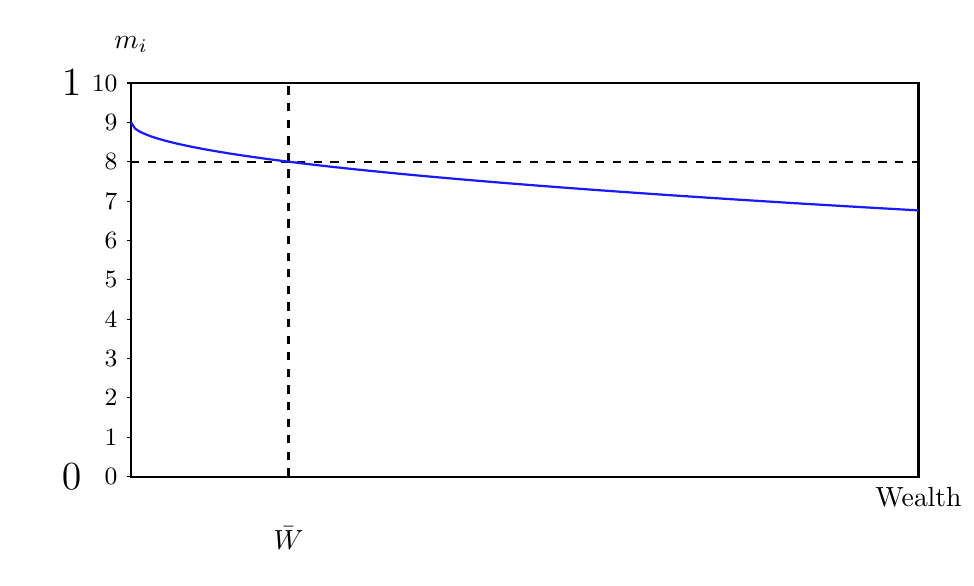
\begin{tikzpicture}[scale=.5]
%\def\bndmax{5}        %https://tex.stackexchange.com/questions/68462/filling-a-complex-region-with-tikz
%\def\bndmin{0.2}
\def\Y{10}  % height of y axis pecent
\def\W{20}  % length  of x axis
\def\Wbar{4}
\def\rbar{8}% this is the prime rate

% %Equation   \[ r_i = (A + .5 \frac{\bar{W}}{W_i})\omega\]
   % \def\Wmin{.63}  %This sets the lower limit fo the 
    \def\Wmin{(\B*\Wbar)/(\Y/\rbar-\A)} %function to keep in in bounds
	
 \tikzset{func/.style={thick,color=blue!90}}	

 \draw [thick](\W,\Y)-- (0,\Y)node[left=.5cm]{\Large$1$}node[above=.25cm]{$m_i$} -- (0,0)node[left=.5cm]{\Large$0$}--(\W,0)node[below]{Wealth}--cycle;  	% Axes box
 
 \draw [dashed, thick] (0,\rbar) -- (\W,\rbar);  	% Axes
\draw [thick,dashed] ( \Wbar,0)node[below=.5cm]{$\bar{W}$} -- (\Wbar,\Y);  	% Axes

\foreach \yi in {0,...,\Y} \draw (0,\yi)--(-.1,\yi)node[left]{\small$\yi$};
%\foreach \yi in {0,2,4,6,8,10} \draw (0,\yi)--(-.1,\yi));
%node[left]{\small$\yi$};
%\foreach \yi in {0,2,4,6,8,10}node at (-.1,yi) {{10*yi}} ;
\draw[func,domain=0:\W] plot [samples=200] (\x,(9-\x^.5/2);

 \end{tikzpicture}
\caption{Individual borrowing ratio $m_i$ as a function of wealth (in tenths)}
 \label{Fig:Borrowingratio}
\end{figure}


\subsection{Individualized borrowing rates}\label{SS:BorowingRate}
 $r_i$ 
 
 $r_i$ should depend on  both the person's income and their assets compared to others. The median after-tax income of Canadian families and unattached individuals was \$66,800 in 2020 according to Statistics Canada's \href{https://www150.statcan.gc.ca/n1/daily-quotidien/220323/dq220323a-eng.htm}{Canadian Income Survey, 2020}.  \href{https://www150.statcan.gc.ca/t1/tbl1/en/tv.action?pid=1110005501}{Data released in 2020 by Statistics Canada} indicates that the top 1\% of Canadians made, on average, around \$512,000 in a single year. \href{https://www150.statcan.gc.ca/n1/daily-quotidien/201222/dq201222b-eng.htm}{Survey of Financial Security, 2019}.

 A study by Statistics Canada found that the typical Canadian household now has a median net worth of \$329,900, while the average net worth in Canada is \$738,200. \href{https://www150.statcan.gc.ca/t1/tbl1/en/tv.action?pid=1110005501}{High income tax filers in Canada}

\subsection{Computing the income constraint on interest rates}\label{SS:YWealthConstraint}
$r_i$

In our model, we  tie the individual cost of capital,  $r_i$ for agent $i$, to a prime rate, $\bar r$ or the bank's target rate, $r^{target}$, prime plus 1\%, say. and to individual wealth. Figures~\ref{Fig:Borrowingrate1} and ref{Fig:Borrowingrate1} illustrate a couple of possible  cost-of-borrowing models roughly consistent  with the stylized facts about lenders. 

\begin{align}
 r_i =  &  \left(A + B \frac{\bar{W}}{W_i}\right) \bar r       \label{eq:incomeandr1}  \\
 r_i =  &  \left(\bar r - A + B *\frac{\bar W}{W_i - C}\right) \label{eq:incomeandr2}  \\
\end{align}
Where $\Bar{W}$ is mean wealth and $W_i$ is individual wealth. In Equation~\ref{eq:incomeandr2},  A determines y-shift, B, the scale, and C the  x-shift for the curve.


\begin{figure}
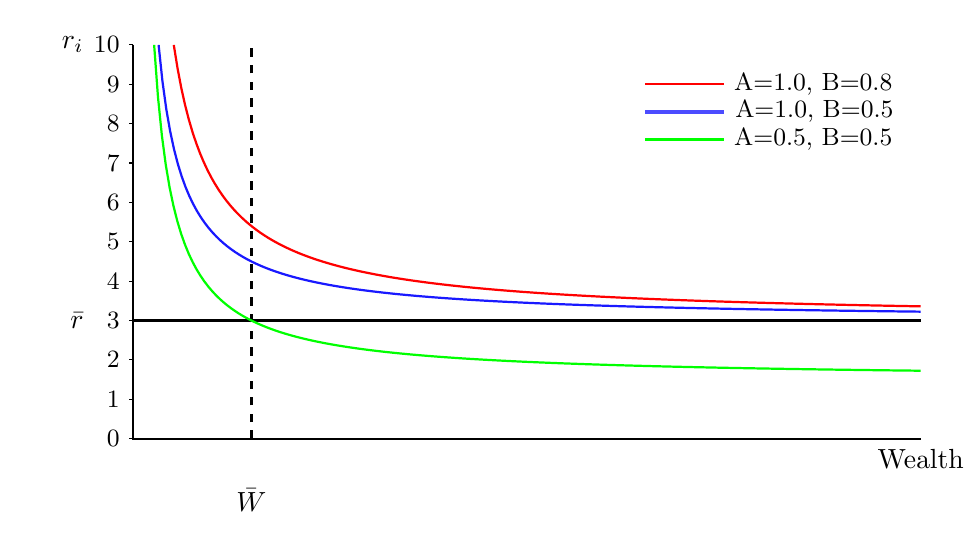
\begin{tikzpicture}[scale=.5]
%\def\bndmax{5} % https://tex.stackexchange.com/questions/68462/filling-a-complex-region-with-tikz
%\def\bndmin{0.2}
\def \Y {10}    % height of y axis as a pecent
\def \W {20}    % length  of x axis
\def \Wbar {3}  % mean wealth
\def \rbar {3}  % the prime rate 

% Equation   \[ r_i = (A + .5 \frac{\bar{W}}{W_i})\omega\]
\def \Wmin{.63}  %This sets the lower limit fo the 
\def \Wmin{(\B*\Wbar)/(\Y/\rbar-\A)} %function to keep in in bounds
\tikzset{func/.style={thick}}	

% Axes
\draw [thick] (0,\Y)node[left=.5cm]{$r_i$} -- (0,0)--(\W,0)node[below]{Wealth};  
\foreach \yi in {0,...,\Y} \draw (0,\yi)--(-.1,\yi)node[left]{\small$\yi$};
\draw [thick] (0,\rbar)node[left=.5cm]{$\bar r$} -- (\W,\rbar);  	% Axes
\draw [thick,dashed] ( \Wbar,0)node[below=.5cm]{$\bar{W}$} -- (\Wbar,\Y);  	% 

\def \A {1.0}  \def \B {0.5} %BLUE
\draw[func,domain=\Wmin:\W, color=blue!90] plot [samples=200] (\x,{(\A+\B*\Wbar/\x)*\rbar});
\draw [ultra thick, color=blue!70 ](13, 8.3)--(15,8.3)node [right, black] {\small A=\A,\ B=\B};

\def \A {0.5} 
\def \B {0.5} % GREEN
\draw[func,domain=\Wmin:\W, color=green] plot [samples=200] (\x,{(\A+\B*\Wbar/\x)*\rbar});
\draw [thick,  color=green](13, 7.6)--(15,7.6)node [right, black] {\small A=\A, B=\B};

\def \A {1.0}  \def \B {0.8} % RED
\draw[func,domain=\Wmin:\W, red] plot [samples=200] (\x,{(\A+\B*\Wbar/\x)*\rbar});
\draw [thick,  color=red](13, 9)--(15,9)node [right, black] {\small A=\A,\ B=\B};
% KEY
\end{tikzpicture}
\caption{Individual borrowing cost as a function of wealth}
\label{Fig:Borrowingrate1}
\end{figure}


\begin{figure}
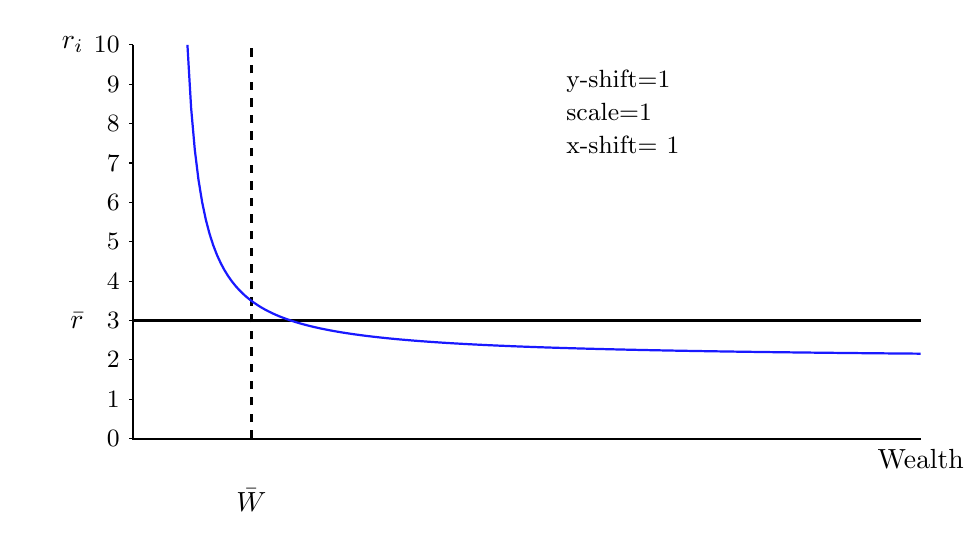
\begin{tikzpicture}[scale=.5]
%\def\bndmax{5}        %https://tex.stackexchange.com/questions/68462/filling-a-complex-region-with-tikz
%\def\bndmin{0.2}
\def \Y {10}  % height of y axis pecent
\def \W {20}  % length  of x axis
\def \Wbar {3} % meam wealth
\def \rbar {3}% this is the prime rate 

%\def \Wmin{(\B*\Wbar)/(\Y/\rbar-\A)} %function to keep in in bounds
\tikzset{func/.style={thick}}	
	% Axes
\draw [thick] (0,\Y)node[left=.5cm]{$r_i$} -- (0,0)--(\W,0)node[below]{Wealth};  
\foreach \yi in {0,...,\Y} \draw (0,\yi)--(-.1,\yi)node[left]{\small$\yi$};
\draw [thick] (0,\rbar)node[left=.5cm]{$\bar r$} -- (\W,\rbar);  	% Axes
\draw [thick,dashed] ( \Wbar,0)node[below=.5cm]{$\bar{W}$} -- (\Wbar,\Y);  	% 

\def \A {1} %vertical shift aroung \rbar, the prime rate
 \def \B {1}  % Scales the exponential curveBLUE
 \def \C {1}  %right shift  
% \def \Wmin {.4+\B}  %This sets the lower limit fo the 
\def \Wmin {(\B*\Wbar)/(\Y-\rbar+\A) +\C} %function to keep in in bounds

\draw[func,domain=\Wmin:\W, color=blue!90] plot [samples=200] (\x,{\rbar-\A+\B*\Wbar/(\x-\C))});
\node  [align=left, text width =2cm ] at (13, 8.3) {\small y-shift=\A \newline scale=\B \newline x-shift= \C};

 \end{tikzpicture}
\caption{Individual borrowing cost as a function of wealth II}
\label{Fig:Borrowingrate2}
\end{figure}

The rates $\delta,\ \sigma,$ and $r$ depend on the period, $T$. 

\section{Incorporating growth and discounting}
%We need a time period T for calculations. For use in any calculation, 

With a price-growth rate of $\dot P$ per year, the growth over $T$ years is $(1+\dot P)^T$, and  %and a 5 year mortgage period, 
the expected price at the end of the period is:

\[P^e_T=P_0(1+\dot P)^T\]

If, for example price growth is 10\%, $\dot P= 0.1$, the {capital gain}, or growth, over a 5-year mortgage term is 0.61051 $\approx$ 60\% of the original price, $P_0$.

If we want the compounded interest rate person $i$ the term T,
\[r_i^T=(1+r_i)^T\]
% This is the value we use in equation~\ref{EqBidPrice}.

If person $i$  discounts at a discount rate $r^\delta$, the present value of a receipt at time $t$ is calculated by using the \textbf{discount factor} $\delta_i^T$.

\[\delta_i^T= \left( \frac{1}{1+r_\delta} \right)^T \]
%\[\delta_i^T= \sum_{\tau=0}^{\tau=T}\left( \frac{1}{1+r_\delta} \right)^\tau \]
 
These can be combined into a function %\delta that  gives a single discounting factor  for a value  like future price that is both growing and being discounted over several (T) periods:
\[ PDV(P^e_T)=P_0\left( \frac{1+\dot P}{1+r_\delta} \right)^T \]
This PDV function specifically combines any expected rent increase, the individual's discount rate and the mortgage term into a single operation.

\subsection{Mortgage availability}
For home loans, many personal finance experts recommend total housing costs account for less than 28\% of your \textbf{gross} household income, This gives us an \textbf{income-based  mortgage maximum} of \[M^{max}_Yi = \frac{0.28*(\omega+w)}{r_i}\] It is the maximum the bank will let you pay.

We assume $r_i$ is based on the individual's assets, on relative wealth. Where is it calculated for the householder or the bank?

We get a \textbf{price-based mortgage maximum} \[M^{max}_P = 0.8P_0\] where $P_0$ is the actual sale price. This is based on the maximum amount of risk that the bank is willing to take on. ($P_0$  will not always be the same as the asking price or the warranted price.)


\section{Table}

\renewcommand{\arraystretch}{1.5}
\begin{tabular}{rlrr}\
Symbol         & Name                                 & Value      & Formula  \\ \hline
$m_i$          & Individual borrowing-ratio           & 0.75-0.85  & $M/P^{ask?}$ \\
$M^{max}_Yi$.  & Maximum mortgage based on income     &            & $\frac{0.28(\omega+w)}{r_i}$ \\
 $M^{max}_P$   & Maximum mortgage based on the price  &            & $0.8*P_0$ \\
$IS$           & Income share for housing debt        & 0.25-0.35  & Missing? \\
$\rho$         & Rent ratio                           &            & $\frac{\omega-tau*d_i}{P_0}$ \\
$\kappa $      & Operations ratio                     & 0.1-0.3    & e.g. $ 0.2\frac{\omega-tau*d_i}{P_0}$ \\
$\sigma$       & Tax ratio                            & 0.25-0.35  & e.g. $ 0.3\frac{\omega-tau*d_i}{P_0}$ \\
$\dot P $      & Price growth                         & []         & $\frac{P_t-P_{t-1}}{P_{t-1}}$\\
$P^T_e$        & Expected price in T years            &            & $P_0(1+\dot P)^T$ \\ % *** WAS $P^e_T$ 
$r_i^\delta$   & Individual discount rate             &            & To assign \\
$\bar r$       & Prime interest rate                  &            & \\
$r_i$          & Individual borrowing-rate            &            & \\
$r^{target}$   & Target interest rate                 &            & $\bar r + margin$ \\
$\delta_i$     & Discount factor for T                &            & $\left(\frac{1}{1+r_i^\delta}\right)^T$ \\
\end{tabular}
\renewcommand{\arraystretch}{1.0}


todo look for $P^e_T$ 

%==========================EXAMPLE=========================== https://www.kaggle.com/code/prateekmaj21/basic-financial-calculations-using-python/notebook
  
% def compound_interest(p,r,t):  %EXAMPLE
    
%     print('Amount: ', p)
%     print("Rate of Interest (Per Annum)", r)
%     print("Time (In Years): ",t)
    
%     a= p*((1+r/100)**t)
    
%     ci= a-p
%     print("Final Amount: ", a)
%     print("Compound Interest: ", ci)
 

\section{Transportation costs}
Transport costs have two parts:
1) fuel and vehicle costs per km
2) time costs per km

\subsection{Vehicle related costs}
Use one year as the wage period, converting transportation costs per km to annual cost for consideration in the household budget. Starting with the cost per km, calculate the cost per year:

\textbf{cost per km =$\textit{t}$}:. \$0.59   (from  Ontario data, 2021). sensitive to congestion, use of subways (\$5 /day?), 

 \textbf{work trips per year} 2 way * 5 days/week * 50 weeks work days = 500. [range: 450-550]

\textbf{cost per km-year} = work trips per year*cost per km

=\$0.59/km*500 trips/year  =  \$295/km year 



\subsection{Time costs}
\textbf{time per km}. range: 20km/hr -> 3min/km, 40km/hr -> (1.5min/km - 3min/ km)per trip 

(New York rush hour is much slower:  4-9km/hr ->6-15 min/km)

\textbf{time  per km-year} = work trips per year*time t per trip = 500* 3min  = 1500 min/km year = 25 hours= 3-3.5 days/km
 
\textbf{time cost per km-year} =  (days per km-year /work days/year)*wage premium per year  = 3/250 = 0.012 years/km year. ?

\textbf{money cost of time per km year} 

=time cost per km-year* wage(including subsistence) 

= 0.012 year* wage per year

\subsection{Total cost per km year of commuting for one agent}
\textbf{money cost of time per km year + \$295/km year * distance} \\
= (0.012 w+ \$295)/km year 
    \begin{quotation}
    \textbf{Example}
    To get a sense of the required wage if we have this annual cost structure, assume city\_extent $d^*$ is 30 km. At this point the transport cost is equal to the wage

\[(0.012 w+ \$295)/km year)*30 =  w\] 
\[.36w+ 8850=w\]
\[w=13828.12\]
        \begin{quotation}
        \textbf{PLAUSIBILITY CHECK}
This is plausible land rent, but does not include building rent. 
Capitalized at 5\% this house is worth \$ 276,562, a fairly cheap house 30 miles from city centre
        \end{quotation}
    \end{quotation}

{\color{red}
\subsection{? Value of $t$ to use in model}}
\[ \tau=(0.012 w+ \$295)/km year \]


% \chapter{Amenity}\label{chapter-amenity}

In this chapter, we discuss how amentity might be treated in this model. 
% from Ricardo_Rent_and_Roemer_3.tex
In our base model,  an urban wage premium is the only labour attractor. Transportation costs to the urban center determine land values. Effectively in our base model, we have set the level of amenities to zero  to focus on the productivity effects. The wage premium provides a reason to find housing in the city and to travel to the city centre to work. Housing choice, however, in reality is always the purchase of a bundle of characteristics such as location, building space, yard, local density and local \glsdisp{amenity}{amenities}. Stegman  found that ``a large majority of families who have recently moved to the suburbs are more concerned with neighborhood quality than with accessibility to other parts of the metropolitan region.'' 
``There is evidence that the amenities offered by a city enhance its growth'' \cite{clarkAmenitiesDriveUrban2002, falckPhantomOperaCultural2011} and that amenity effects themselves scale superlinearly \cite{kraemerCulturalSustainabilityUS2022}.

Kaufmann et all \cite{kaufmannScalingUrbanAmenities2022} investigated the general statistical patterns in the quantity and spatial distribution of different urban amenities including public spaces and institutions as well as businesses, which all provide different services to urban populations, such as restaurants, parks, or universities.  They argue that amenities are in fact central for generating and supporting economic agglomeration effects, attracting investment to ``developing neighborhoods, promoting economic growth, supporting innovation clusters and facilitating businesses linkages.'' 
They show that the aggregate quantity of amenity infrastructure (not amenity supply)  in an urban area scales sub-linearly with population size across US metropolitan areas.\footnote{When they disaggregate, however, they find that for approximately 74\% of amenity types, they cannot reject linear scaling. Four percent exhibit super-linear scaling. They list take-away restaurants and travel agents in this range. Sub-linear scaling is associated with libraries, universities, and movie theatres.} This strongly suggests there are scale economies in amenity provision.\footnote{The model they use is the same as the one used to demonstrate that a scaling law holds for urban GDP. Instead of GDP, however, the dependent variable is a measure of amenity density based on data extracted from a unique new Google Places dataset, Google Places API (2012).} 


The amenities offered by a city can be seen as a form of non-market, non-monetary income \cite{kaufmannScalingUrbanAmenities2022}.  The non-market component of household incomes affects choices. Greater consumption amenities in a city will make workers willing to accept lower wages or higher rents. For firms,  lower wages mean lower costs. Thus,  higher amenity levels may lead to lower money wages as workers trade amenity for money income. With lower wages, more workers can be hired leading to higher output and a larger population \cite{pugaMagnitudeCausesAgglomeration2010}. 
When positive urban amenities prevail, rents and housing prices will be higher in larger cities, but wages may be unaffected \cite{robackWagesRentsAmenities1988, dalmazzoAmenitiesSkillbiasedAgglomeration2011}.
%localized productive advantages will make firms willing to accept higher wages and higher rents  


%It involves budget allocation. If we hold the housing budget constant and add an explicit urban amenity, other variables must adjust. 
% Higher wages make residents better off whereas higher rents make them worse off. Thus, 


%.  This helps disentangle the consumption amenities from the productive advantages of big cities.


In our base model,  To introduce amenities we can simply add an amenity value $A$ to the estimated value of any home. The value can depend on location, allowing for `better' and `worse' neighbourhoods,  and it can be made to depend on household attributes: a family with children might value a neighbourhood with a school or a park more highly. 

For some households, the amenity of an area may depend on the density of the city or of certain types in a neighbourhood. This is a social agglomeration effect that may work in addition to the agglomeration effect on production \cite{gurwitzCatastrophicAgglomeration2019} that we have already considered. There are also agglomeration effects in consumption goods. Larger consumer markets support more variety in goods and services. This variety allows a greater range of preferences to be satisfied. A larger city may have more production sectors and a larger array of consumer services, increasing the value received from a given income.  These closely related but different effects can be modeled by introducing an amenity term in various ways 

The amenity-induced rise in housing prices may absorb what would otherwise be consumption expenditure on other goods. Residents might accept smaller housing units for access to urban amenities.\footnote{Some costs may fall with agglomeration. There is evidence of a strong negative correlation between the total energy consumption of a city and its overall urban density \cite{newmanSustainabilityCitiesOvercoming1999}. Larson et al. \cite{larsonEnergyImplicationsCity2015} show that per-capita energy use is relatively invariant to city size when growth is driven by wages but falls modestly with growth induced by rising amenity.} In any case, there will be distributional effects as amenities play a larger role in urban agglomeration. Property owners will capture increased land rents. If amenities are funded out of taxes, the burden falls on all residents, since property taxes are very roughly related to housing consumption, but the land rents are captured by institutional owners as well as owner-occupiers and not by tenants.


%\glspl{amenity}, or non monetary income it another form of wealth,See Kaufmann et al. \cite{kaufmannScalingUrbanAmenities2022}.  and it is %, are however, an important feature of the urban system. 
% We have intentionally suppressed amenity but can add it it simply.
% (ownership effects, produtivity spilllovers, - table where you show them in the static and dynamci case with amentity)
% 2 classes of exploratin of the model in the past tho chaptered

 
%To understand amenity in our model, we need to understand it's relationship with growth, productivity, and agglomeration.
\section{Modelling amenity}

This section sketches an extension of the model to study include \gls{amenity} and suggests how it might affect results. Amenity effects can be introduced in a variety of ways. %hey might work though An economics might prefer to introduce amenity as a good in the utility function of agents.
% It might then depend on the size of the city, the size of an amenity-producing sector, the specific amenity-generating infrastructure provided by the city through taxes,  or neighbourhood effects. Each of these would take a different functional form. In our model agents are represented by their demand for housing, so the same terms would be introduced into the bid function. % In the utility framework, bids are simply derived from the utility function, so the two approaches are equivalent. %  The virtue of using the utility framework is that it begins with the question, ``What do people want?'' rather than ``What do people do?'' The first question is more productive if we want to identify different amenities that might matter.

\subsection{Through household utility}
The most direct way to incorporate agglomeration amenities is  to include what might be called a \gls{utility premium} for urban dwellers as non-monetary location income $\mathbb{A}(d; N), \die{\mathbb{A}}{N}> 0), \die[{\mathbb{A}}]{d}< 0)$ depending on distance, $d$ from the centre and urban population $N$. The second term can incorporate local amenities as well. A simple linear (indirect)\footnote{The indirect utility function is a function that depends on income and prices rather than goods and services.  Income does not generate utility, but it does generate utility indirectly' because it enables people to purchase goods and services.} utility function specified on broad income (net wage plus locational amenity) is convenient for illustration:

\begin{equation}VU(w,A)= \psi+ \omega-cd + \mathbb{A}(d; N) - T(d))
\label{eqn-u}
\end{equation}
where $w$  is an urban wage p, $T(d)$ is transportation cost from the centre to $d$.
\footnote{\cite{anasUrbanSpatialStructure1998} shows that a linear transportation cost will not  hold if congestion declines  with $d$.} 
 In most versions of the Alonzo model the `wage premium' is simply given in the urban wages and there is no amenity term. 


%\footnote{wage income, if all income goes to housing, or the share of wage income going to housing services.   (If we use a Cobb-Douglas utility function we would just replace $w$ with    $\alpha Y$, where $Y$ is household income and $\alpha$ is the share of total income. } Let  $T(d)=td$ be transportation cost with  $t>0$. 
 
\begin{figure}[t!b]
\begin{center}
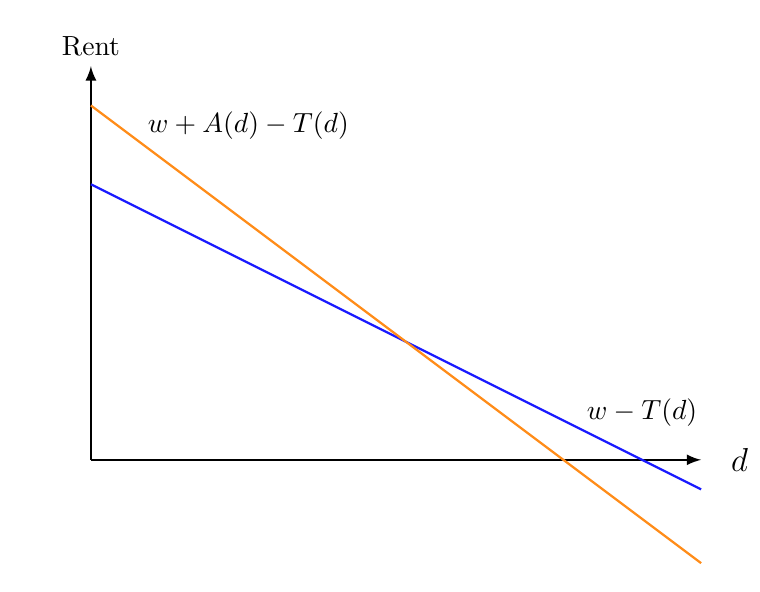
\begin{tikzpicture}[scale=.5]
\def\bndmax{5}        %https://tex.stackexchange.com/questions/68462/filling-a-complex-region-with-tikz
\def\bndmin{0.2}
\def \n {10}
\def \m {15.5}
\def \t {.5}
\def \th {1}
\def \w {7}
\tikzset{func/.style={thick,color=blue!90}}	
\draw [thick, latex-] (0,\n)node[above] {Rent}--(0,0);
\draw [thick, -latex] (0,0)--(\m,0)node[right=.25]{\large $d$};
%\foreach \xi in {0,..., \m} \draw (\xi,0)--(\xi,-.1)node[below=1]{\small$\xi$};
%\foreach \yi in {1,...,\n} \draw (0,\yi)--(-.1,\yi)node[left]{$\yi$};
%%\foreach \i in {1,4,9,16} {
	\draw[func,domain=0:\m] plot [samples=200] (\x,{\w-\t*\x});
%	\draw[func,domain=0:\m, dashed] plot [samples=200] (\x,{\w+\azero-\th*\x+\aprime*\x});

\node at (14,1.2){$w-T(d)$};
\def \azero{2}
\def \aprime {-.25}	
\tikzset{func/.style={thick,color=orange!90}}	
	\draw[func,domain=0:\m] plot [samples=200] (\x,{\w+\azero-\t*\x+\aprime*\x});
\node at (4,8.5){$w +A(d)-T(d)$};
%\node at(-.8,2) [left]{base $2^1=$};
%\node at(-.8,1) [left]{$2^0=$};
%\draw[dotted] (0,2)--(1,2)--(1,0); 
 \end{tikzpicture}
\end{center}
\caption{Rent profile with amenities}
\label{fig-amenity}
\end{figure}

 This model can produce variations on the standard result in the Alonso model. Figure~\ref{fig-amenity} illustrates a linear amenity function, $\mathbb{A}(d|N)= a-b*d$, that is convenient for illustrative purposes.  It shows how a particular amenity function might affect the rent profile, and hence city size and it allows simple experiments with the effect of increasing population on city size, wages and rents. 

In this case, amenity falls below zero in the outer regions of the city and, the geographical size of the city will be smaller. With a linear function, this happens if $\frac{a}{b} < \frac{w}{t}$. (a smaller city would have a secondary effect on wages, since with fewer workers' marginal productivity would be higher and therefore wages would rise. This would partially offset the initial decline in population.)
There would be a band of land around the city with negative amenity for commuters.\footnote{The very simple graphical result rests on several assumptions - no other housing expense, housing all the same size, wages all equal, preferences identical, transportation costs.}

The far more likely case is that $A(d) > 0$ when $w-T(d)$ falls to zero. In this case there is a band of residents around the city, outside of the population commuting to work. They do not travel to work,  do not collect a wage, but still enjoy the amenity of being close to a city. This might be a population of retired persons enjoying occasional visits and healthcare facilities.


\subsection{Neighbourhood amenity}
In Figure~{fig-amenity} the source of the amenity is at the centre of the city. We can easily imagine an amenity profile that is high for some neigbourhoods and lower for others, as in  In Figure~\ref{fig-amenity2}. The jagged area below the orange line is rent accruing to landowners. The variable rent comes not from a desire to be close to the source of the wage income but from household demand for local amenity.  
\begin{figure}[tb]
\begin{center}
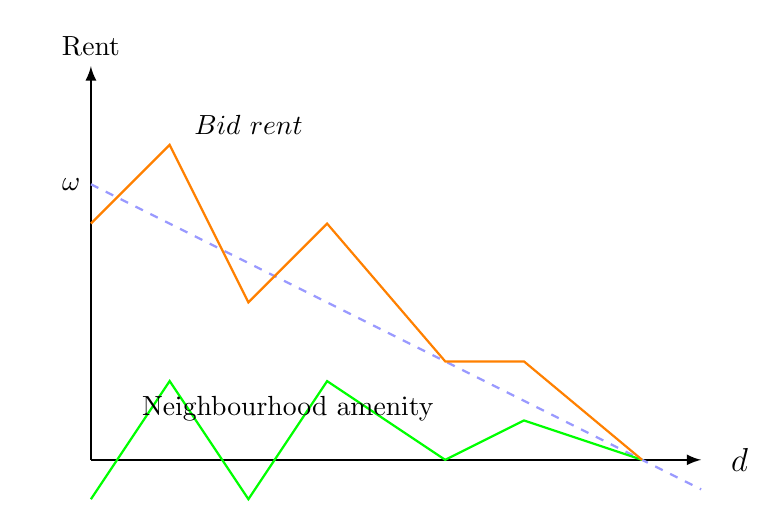
\begin{tikzpicture}[scale=.5]
\def\bndmax{5}        %https://tex.stackexchange.com/questions/68462/filling-a-complex-region-with-tikz
\def\bndmin{0.2}
\def \n {10}
\def \m {15.5}
\def \t {.5}
\def \th {1}
\def \w {7}
\tikzset{func/.style={thick,dashed, color=blue!40}}	
\draw [thick, latex-] (0,\n)node[above] {Rent}--(0,0);
\draw [thick, -latex] (0,0)--(\m,0)node[right=.25]{\large $d$};
% Basic Bid rent,
\node at(-.5,\w) {$\omega$};
\draw[func,domain=0:\m] plot [samples=200] (\x,{\w-\t*\x});
%NEIGBOURHOOD AMENITY
\draw [thick, green] (0,-1)--(2,2)--(4,-1)--(6,2)--(9,0)--(11,1)--(14,0);
\draw [thick, orange] (0,6)--(2,{7-2*.5+2})--(4,7-4*.5 -1)--(6,7-6*.5+2)--(9,7-9*.5)--(11,7-11*.5+1)--(14,7-14*.5);
\node [] at (5,1.3){Neighbourhood amenity};
\def \azero{2}
\def \aprime {-.25}	
% \tikzset{func/.style={thick,color=orange!90}}	
% 	\draw[func,domain=0:\m] plot [samples=200] (\x,{\w+\azero-\t*\x+\aprime*\x});
\node at (4,8.5){$Bid\ rent$};
%\node at(-.8,2) [left]{base $2^1=$};
%\node at(-.8,1) [left]{$2^0=$};
%\draw[dotted] (0,2)--(1,2)--(1,0); 
 \end{tikzpicture}
\end{center}
\caption{Rent profile with neighbourhood amenities}
\label{fig-amenity2}
\end{figure}
Financialization might or might not affect neighbourhood amenity. If it does it might have its effect by changing the ownership mix.

\subsection{Public provision of amenities}

Previous sections suggest amenities may work as a wage subsidy, potentially increasing output. Since employers will not willingly pay for urban amenities, some amenities may be financed publicly. It is common to introduce the cost of generating amenities as a tax on residents.  Since public amenities may be \glspl{public good} in the economic sense, the municipal government may be able to achieve significant wage economies with a small public expenditure.

A simple way to incorporate publicly provided amenities to make an amenity function that proportional to a fraction of public revenue, which is a fraction $\tau$ of the land value when municipalities depend on property taxes. Assuming a uniform property tax rate, total property tax revenue in a circular city are approximately $\tau(\phi+2/3 \omega)\pi \frac{\omega}{c}^2$. We can therefore include in the buyer's maximum bid function a fraction if this value. Property investors would not include this amenity component, but it would affect their decisions because amenity raises their net rent.

Notice that because amenity raises property values, in Ontario it does not raise tax revenue because the property tax rate is adjusted to balance the budget. This creates perverse incentives for municipalities \cite{blaisPerverseCitiesHidden2011}.


\subsection{An amenity sector}
Producing amenities takes resources. Some fraction of the workforce must be engaged in producing the amenity services. A simple approach would be to assume that the base employment that we consider demands a layer of amenities that represent the additional fraction of the population needed to provide the amenities - say 10\%  

Larger cities can support larger and more varied amenities, so that effect of amenities on property values might be larger in larger cities. At the same time, there are apparently economies of scale in the production of amenities \cite{kaufmannScalingUrbanAmenities2022}. We have no strong prior about how in amenity sector would be affected by finacialization of housing.  An effect might work through changing ownership.


\section{Research on amenities}
% There is a great deal of research on amenities. In this subsection mention a few that seemed noteworthy. 
Most of the literature on amenities deals with livability and the benefits for the individual. There is a strand in the literature, however, that links amenities to growth. In 1954, for example, Edward Ullman \cite{ullmanAmenitiesFactorRegional1954} published  ``Amenities as a Factor in Regional Growth,'' an article that came to be seen in the geographical literature over the following 50 years as prescient \cite{walcottCommentsEdwardUllman2010} for introducing the notion that amenities could be an important mobility magnet. 

Many have since extended this approach. Richard Florida, in a series of articles and books beginning in 2002 \cite{floridaCreativeClassEconomic2014, floridaEconomicGeographyTalent2002, floridaCompetingAgeTalent2005} examined the notion that urban growth depended on attracting the creative class and that in turn rested in part on the amenities a city offered. A 2008  Statistics Canada study, `Cities and Growth: The Left Brain of North American Cities,' Beckstead et al \ found substantial differences in average growth for cities with higher cultural employment and urban amenities.  Clark et al \cite{clarkAmenitiesDriveUrban2002} argue that much of Chicago's recent growth to 2003  should be attributed to reforms instituted by Mayor Richard M.  Daley explicitly linked to amenities and quality of life issues, including parks and schools. Abouy \cite{albouyWhatAreCities2016} finds that wage and housing cost differences across metropolitan areas are accounted for more by productivity than quality-of-life differences, however. 

Beckstead et al  \cite{becksteadCitiesGrowthLeft2008} identify amenities with the unexplained variastion in median urban house price after controlling for median household income.\footnote{  The basic premise would be that after conditioning on household income, variation in home prices across cities would be a function of the relative attractiveness of these places. The residuals yield a continuous ranking of cities based on the estimated variation in urban amenities.} Rappaport \cite{rappaportConsumptionAmenitiesCity2008} presents empirical evidence that amenities do support high-density levels, and that amenities cause approximately one-fifth of the cross-sectional variation in metro population density. 


% Molotch's (1976) metaphor suggests that the city is a machine geared to creating growth, with growth loosely defined as the intensification of land use and thus higher rent collections associated professional fees and locally based profits. Many urban economists, planners, and political scientists have made similar arguments (e.g., Bradbury, Downs, & Small, 1982; Mollenkopf, 1983; Stone, 1989). However, a quarter century later in the contemporary competition among US cities, the growth machine model has lost much of its power.
  


\newpage


% \chapter{Notation}
% \section{Notation for Urban and Production Sectors}
\newpage
\begin{longtable}{lp{10cm}}
\caption{Notation}                       \\
\hline           &  \textbf{Productivity} \\ \hline
$K$              &  Capital               \\ 
% $L$            &  Labour                \\
$N$              &  Population, equals labour \\ %, $L$          
%$\Lambda$    &  Labour-augmenting agglomeration effect \\
$Y=A K^{\alpha }N^{\beta }$  &  a Cobb-Douglas Production function \\ %Urban output            \\
$\alpha$         &  Elasticity of output with respect to capital          \\
$\beta$          &  Elasticity of output with respect to labour           \\ % vs effective labour
$\gamma$         &  Elasticity of agglomeration with respect to labour    \\ % , $\Lambda(n)$, for illustration \\

% $L$              &  Labour supply \\ %the number of workers, which, in the standard circular city model, equals the number of lots of size $s$  when workers live on identical individual lots. % Unless $d^{max}>d^*$ v  \frac{\pi}{s}(\frac{w}{{c}})^2 =
$n$  &  Number of workers at a firm \\
% $n_i$  &  Number of workers employed by firm $i$ \\
%$n=\sum_i n_i$  &  Number of workers, the urban population in the model \\
% $\#f=\frac{n}{n_i}$&number of identical firms \\ %not used
% $f$  &  Number of firms =1 \\
% $n =f n_i$  &  Aggregate labour \\
% $n^\gamma$ & The labour-augmenting agglomeration effect,  modelled as an exponential function of the number of people \\
% $\Lambda(n)n_i$ &  Effective labour for firm $i$ \\
% $\Lambda'=\die{\Lambda(n)}{n} $ & Derivative of the labour-augmenting agglomeration effect\\

%%$Y_i=K_i^{\alpha }(\Lambda(n)n_i)^{\beta }$  &  Urban firm $i$'s output \\

%%$Y=\frac{n}{n_i}K_i^{\alpha }(\Lambda(\sum_i n_i)n_i)^{\beta }$  &  Aggregate output of all firms in the city \\
% $\die{Y}{n}=\beta\frac{1}{n} Y  \left( 1+ \frac{n\Lambda'}{\Lambda} \right)$  &  Social marginal product of labour \\
% $Y_i=K_i^{\alpha }(\Lambda(n)n_i)^{\beta }$    &  Urban firm $i$'s output \\
% $\die{Y_i}{K_i}	=\alpha \frac{1}{K_i} Y_i $  & Marginal product of capital for firm $i$ \\
% $\die{Y_i}{n_i}	=  \beta\frac{1}{n_i} Y_i $  &  Marginal product of labour for firm $i$ \\
%%$\eta=\frac{n_i\Lambda'}{\Lambda}$  &   Marginal agglomeration effect on a firm's output of increasing it's own labour stock \\
% \hline
	% &\textbf{Amenity}\\ \hline
% $A(d, n)$   &  Agglomeration amenity          \\

\hline  0 &  \textbf{Labour market}                \\ \hline %and urban stucture??
$\psi$            &  Rural subsistence wage                             \\  
$\omega$          &  Urban wage premium          \\
${c}$             &  Transportation cost per unit distance \\ % Was $\tau$, and $trans$. Considered $\gamma, \xi, \zeta$.
$d$               &  Distance from city centre   \\
$d^* = w/{c}$     &  City extent \\ %, the maximum distance commuters will travel \\ % Maximum distance commuters will travel \\ % to get the wage premium \\
% $\mathcal{R} = \omega - {dc}$ &  Rent at distance ${d}$ \\ 
% $\zeta$          &  Population density at distance $d$     \\
% $s$              &  Lot size      \\
% $\psi$  &  ?Per-period cost of a unit of productive capital \\
% $\omega + \psi$  &  Urban wage including rural wage \\ %***
% $\textit{t}$ & {\color{red}transportation cost per km} \\%use   c?
% $w^n=\omega-{dc}$ & Wage  premium net of transportation costs \\
%% $\Omega=\frac{\omega+\psi}{\psi}$  &  Ratio of the urban wage to the  cost of capital \\
%% $\Pi$	   &  Profit \\
%% $ER$	   &  Excess return to capital \\ 
% \hline &\textbf{Spatial structure in the circular city} \\ \hline		
%% $d^{max} = \omega /{c}$  &  Maximum distance commuters at which residents enjoy the urban amenity \\
%% $d^{**} = max(d^*, d^{max})$  &  radius of the city \\
%% $U$                     &  Worker utility **\\ %, a function of location and prices \\
%% $U^{urban}=U^{rural} $  &  Migration equilibrium assumption ** \\
% \hline & \textbf{Labour market} \\ 

\hline           & \textbf{Financial market}             \\ \hline
$P_W$            &  Warranted price for a property       \\
$P_B$            &  Bid price                            \\ % was P^{bid}
$P_A$            &  Asking price                         \\
$P_M$            &  Realized market price                \\
$P_M^e$          &  Expected market price                \\
% $P$            &  Price of a property                  \\ 
% $\dot P$       &  Rate of price growth              \\ % was $\dot p$  
% $\mathcal{C}$    &  Capital gains                     \\ % was C
% $\mathcal{C}_N$  &  Net capital gain, $C -$ net rent  \\
% $M$              &  Mortgage                          \\ 
% $m$              &  Mortgage share, the share of the property price that can be borrowed, which is a function of wealth  \\ 
$\mathcal{R}$    &  Rent                              \\
$\mathcal{R}_N$  &  Net rent                          \\
${R}^w_N$        &  Warranted rent                    \\
$\rho$           &  Rent ratio                        \\
$\phi$           &  \Gls{rent share}                  \\
$\mathcal{O}$    &  Operational costs                 \\
% $\theta$         &  Operations ratio                  \\ % was $\kappa$ became b
$\mathcal{T}$    &  Taxes                             \\ % was $\Sigma, \Xi$  
$\tau$           &  Property tax share                \\ % was t then $\sigma, \xi$  b
% $\tau$            &  Annual tax rate on rent and home \\ % Was $c$ 
$r$              &  Interest rate                     \\
$\delta$         &  Individual's subjective \gls{discount factor} \\
% $W$            &  Wealth                            \\
% $\psi$         &  Fraction with rent/operating costs\\
$t$              &  Time                              \\

W & Wealth \\
m & Mortgage share \\
M & Mortgage \\
S & Savings \\
% \mathbb{C} carrying 0.28, max_mortgage share, wealth_sensitivity

$\mathbb{T}$     &  Time period                       \\

$a$       &  Share of subsistence wage  used for land and building \\
$b$       &  Maintenance share of share of subsistence wage \\ % A cost. Includes water, electricity, heat? 
% $wage_share$     & OLD Share of the agglomeration effect that goes to workers. \\

\hline
\color{black}
\end{longtable}  

\newpage

\begin{longtable}{lp{10cm}}
\caption{Rent}                                                            \\
\hline
$\omega-{dc}$                &  Warranted (economic) rent                \\
$\mathcal{R}=\omega-{dc}$    &  Equilibrium rent payment of tenant       \\
PDV                           &  Present discounted value                 \\  
$\mathcal{R}^T$               &  PDV of rent collected over period $T$    \\ 
$\mathcal{R}^T_N=(1-\kappa-\sigma)\mathcal{R}^T$  &  PDV of net rent collected over period $T$ \\
\hline
\end{longtable}

\begin{longtable}{lp{10cm}}
\caption{Bidding mechanism notation}                                          \\
\hline
$\mathcal{R}_N$  &  Net rent                                                  \\ % was NR
% $P_0$            &  Purchase price for a property                             \\
% $P^T_e$          &  Expected price at the end of period $T$                   \\
$r^{prime}$         &  Prime interest rate                                       \\
$r^{target}$     &  Investor or banks target interest rate, $\bar r + margin$ \\

$r_i$            &  Agent $i$'s personal borrowing rate                       \\
$r_i^T$          &  Agent $i$ interest rate compounded over a period $T$      \\
$r_i^{disc}$     &  Agent $i$'s subjective discount rate (which may equal $r_i$) \\
$r_\delta$       &  Discount rate                                             \\ % was $discr_i$
$\delta_i^T$     &  Discount factor for agent $i$ over period $T$             \\
$m^W$            &  Wealth-based share of home price a worker can mortgage    \\ % $= m_i(W_i)$
$m^\omega$       &  Income-based share of home price a worker can mortgage    \\ % IS_i   IS_i(\omega+\psi)$$
$m_i = min(m^W_i, m^\omega_i)$  & Mortgage, the share of home price worker $i$ can mortgage \\

\hline
\color{black}
\end{longtable}  
Notation: 
Agent counts and indices are subscripts.
Values related to time are superscripts, time as a continuous 
variable is small, a period is capitalized e.g. the period $T$ of some number of years. 
In general values are capitals, rates are small letters.

% It might be better to use the subscript $m$ for `market'.  for warranted rents



 

% % Short
% % \chapter[Future Work]{Future Work}
\label{appendix-future-work}



In  this chapter, we discuss potential extensions of our basic model.  Models are by nature combinatoric: every added element involves making a choice among alternative assumptions and implementations. A model incorporating in binary choices is one of an implicit family of $2^n$ alternative models. We have sharply restricted our model  in order to focus on one process of significance, financialization.  This is in part so that we can explain and justify each assumption that we use, and in part because only sharply restricted models produce understandable results. 
% Those results are condition on the specific set of assumptions to ensure that 
We have designed the model to  accommodate a range of extensions that are either theoretically or interesting or important for policy-makers. 



Figure~\ref{fig-logic-extensions} illustrates  five general types of extension. The first is to move from a static population to a model with population pressure. This appears on the left as a group of three new subroutines with connections to the elements of the model most directly affected. Some links are left out to keep the figure readable. Examples of omitted links  are the channels through which  population affects labour supply and savings.  


A second class of extension would introduce a housing production sector. This appears on the right side of of the figure linked to the banking sector. It requires adding a dynamic housing  stock. 

A third major class of extensions, separable from production is to introduce variation of housing form,  density and amenity. Zoning restrictions and building codes are related. Many questions about who gets what housing arise at this point. 

{\newpage\thispagestyle{empty}
\vspace{-1.5cm}
\begin{figure}
\vspace{-4.5cm}
\begin{adjustwidth}{-0.24\textwidth}{-0.2\textwidth}
\centering
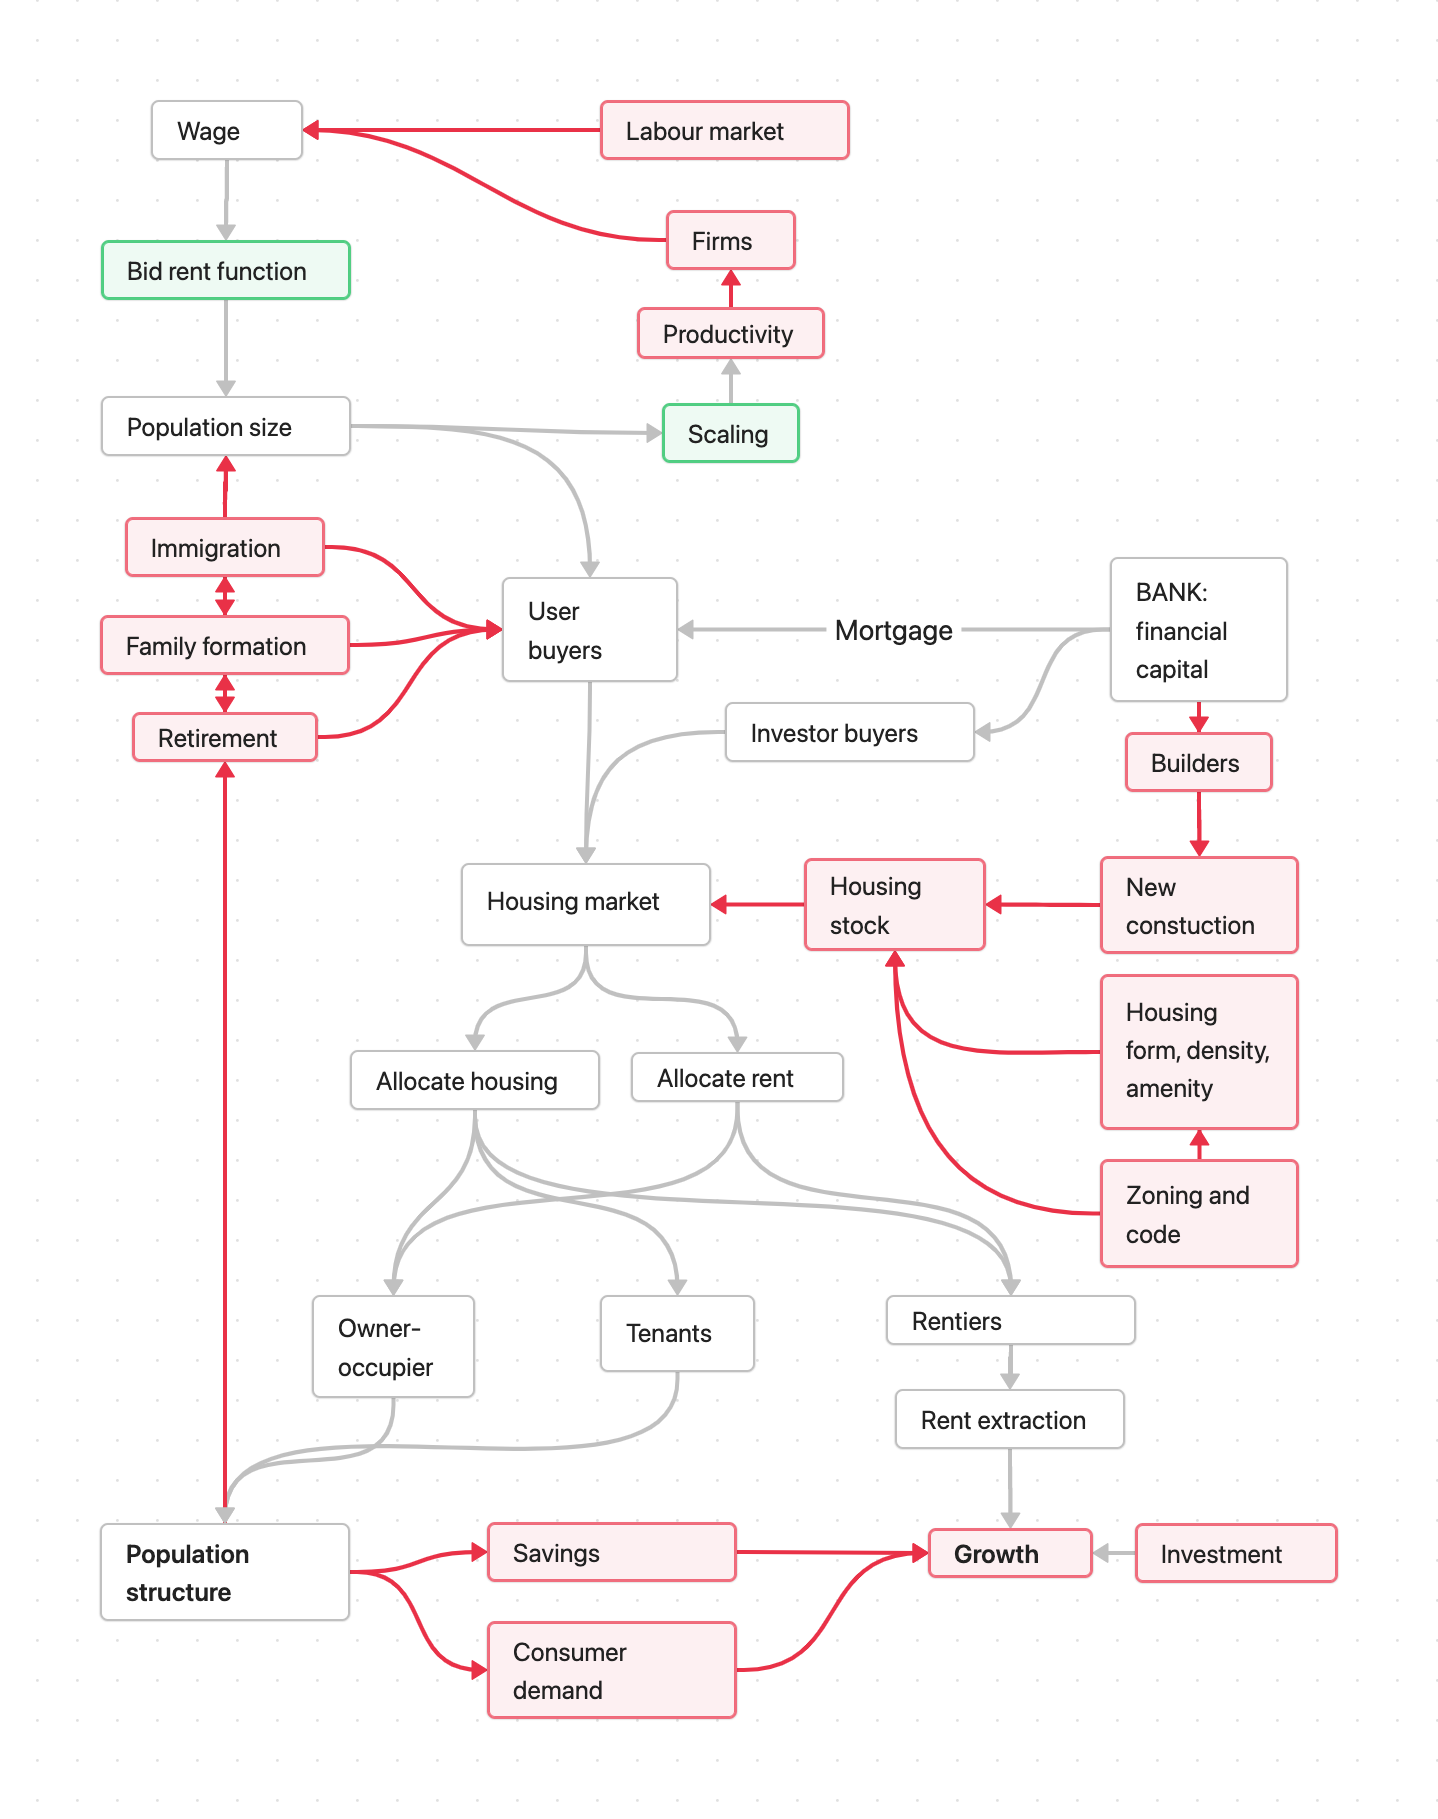
\includegraphics[scale=.22]{fig/extensions.png}
\end{adjustwidth}
\caption{Extensions}
\label{fig-logic-extensions}
%\pagestyle{headings}
% \usetikzlibrary{positioning}
%\begin{tikzpicture}[remember picture,overlay,shift={(current page.north east)}] \node[anchor=north east,xshift=-1cm,yshift=-1cm]{\includegraphics[width=1cm]{example-image-a}};\end{tikzpicture}

\end{figure}
}


At the bottom of the figure we introduce consumer demand linked to the population structure and feeding back to growth. Savings behaviour becomes more  complex when consumer demand is made endogenous and with as more complex population structure.

The fifth block of extensions illustrated in Figure~\ref{fig-logic-extensions} would replace the simple, scaling-based transmission mechanism in the Alonzo-Jacobs cycle with explicit firm and labour market behaviour. This class of extensions is obviously linked to population structure. It leads to consideration of firms that produce different products, some for export some for the local market, and to multiple types of labour.

Linked to the labour market and production system is the possibility of introducing competing cities. 

It should be clear that each of the extensions we suggest is potentially as complex as our core model, and each brings with it a collection of additional assumptions. We would argue that none of them would change our qualitative results greatly, although each would deepen our understanding of mechanisms and of the detailed impacts.


\section{Population pressure } 
Our basic model does not have a growing population. This conveniently allows us to isolate certain effects of financialization. Population pressure is one of the drivers of financialization because it amplifies speculative gains, however. As a result, one of the first extensions must be  to introduce population pressure.

There are two sources to consider: 
\begin{enumerate}
\item agglomeration effects that increase the wage and attract workers faster than the housing stock can respond. 

Worker agents from outside the city can always consider moving and accepting a job. 
% QUESTION - how to manage the flow of new agents?
%, or can make more from rents and moving away
\item immigration pressure
\end{enumerate}
under the  first, agglomeration economies drive population while under the second, population growth may drive agglomeration.

The growth of the housing stock will generally lag population growth, generating price effects and stock dynamics.

Agents will respond to increases in demand conditions. The perception that the market is tight or that prices are rising may lead to higher bids and reservation prices and shift results in favour of sellers.  


%Buyers could consider neighbourhood pressures, demographic changes, changes in job location, desire for amenity etc. in their assessment of housing need. 

%With multiple bids agents can place the most competitive bids on those homes they prefer. If they have higher urgency they place strong bids on more homes. 

%Next buyers request a selection of homes to consider from a real estate agent. Those with higher need for housing look at more homes. The real estate agent offers a selection of homes based on the agent's requirements. A randomness parameter determines how many divergent houses are also considered. When the parameter is 1, the selection of homes is fully randomized, When it is 0, the agent sorts all available homes and offers those which fit the agents budget, space, and other requirements best.


\subsection{Retirement investors and private investment properties}
The simple population turnover in our model can be replaced with a more complex set of possibilities at the agent level.  At retirement,  agents can be allowed to may choose between selling their home, renting it as an income property, or if there is sufficient amenity value for them, staying in the city. Implementing these choices complicates the agent decision and the resulting housing distribution but require few changes to the rest of the model.

\section{Housing production}

\section{Differences in density, housing form, and neighbourhood amenity}
Much of what is interesting in a city is the rich variety of housing forms and neighbourhoods and the varied populations that occupy them. Our model has a single form of housing and an undifferentiated populations, allowing us to differentiate the housing system in specific ways and study the interactions between the built world and the population. We are convinced that few of the possible extensions could affect our qualitative results. 

Nonetheless, in our agent based model, in which every lot is  addressable, it is simple to introduce zoning boundaries, local amenities, different densities or housing qualities and homes of different sizes. Hundreds of experiments are possible exploiting  the extensibility we have carefully conserved.  

We can ask what would be the effect of a hard zoning boundary and what would be the effect of suddenly relaxing it. We could explore the effect of speeding the rate of conversions from one size  home to another, or of locating high density pocket on a transportation route. Many significant urban policy questions could be examined with a limited amount of additional programming. 

\section{The consumer city}
Much of the demand for what is produced in the city is local consumer demand.  Our model has assumed there is production only for a perfectly elastic export demand. Consumer needs are buried in the subsistence wage. 

A minimal extension would be to introduce a second sector representing local consumption demand. A share of locally generated income would support production for the city's population. The labour force would be split between the two sectors and both productivity and wages might differ across sectors. 

A more complex treatment would introduce a range of service, entertainment and retail producers. This might be done monopolistically competitive firms \'a la Dixit and Stiglitz \cite{AvinashK.Dixit1977MCaO}.



\subsection{Distribution of rents}
Rents go to landowners, with a share taken for maintenance and taxes.
Rents may also be taxed, could be shared between multiple owners, etc.
 %\note{REPHRASE? rent is  extracted from the coalition of capital and workers.} % Rents may also be taxed, could be shared between multiple owners, etc. 
%The rents are captured by landowners.  The capture of rents by landowners is common buy not necessary. 
In principle the gains from urban productivity and amenity can be allocated as social wealth through shared ownership, as is often done on a small scale with cooperatives and land trusts, distributed to all citizens through something like a social wealth fund, or captured in taxes or fees as Henry George suggested. 
%The rents would otherwise go to labour and capital.





\subsection{Urban Savings - Contributions?}
THIS IS A CONTRIBUTION, BUT ALSO A DISCUSSION OF ONE WAY THIS WORK COULD BE EXTENDED, MIXED WITH A BIT OF MODEL DESCRIPTION

Conventional growth models specify a savings/investment mechanism at the national level. To our knowledge, this has not been done for the city level. We require  savings at two levels. First, since we want to incorporate  households home ownership and a relationship to the financial sector through mortgages, We specify a savings rate out of the spending we have isolated in the `subsistence wage' This means that both urban and rural workers accumulate savings, that savings are age-dependent, making the size of mortgage available also age dependent. 

Homeowners in addition have equity $E=P-M$ in their homes.  ({\color{red}Should newcomers also have equity? or is it built into the savings. Clarify this.} 

A second level of saving is the  investment in capital out of the city surplus. Even raising this question puts us into terra incognita. There are many  channels through which surplus flows into productive investment in the urban contest. One is through public investment in infrastructure. We have discussed how falling transportation costs increase surplus generation. Investments like this are made slowly and take effect over time periods much longer than our model is concerned with.  We can set a property tax rate   that we will assume is sufficient to maintain the stock of infrastructure.

Public and private investment in human capital is largely urban as well, but as with infrastructure, investment and response take effect over time periods much longer than our model is concerned with. 

Private sector innovation in technology, marketing, or products draws on local saving less but still significantly on local savings. We have little in the way of theory or empirical research on this channel. Lags between investment and any rise in the urban wage premium are almost certainly long and variable. 

We deal with this issue by linking local capital ownership with the scale factor. It is known that local ownership is associated with local investment. We will assume that local capital ownership, which consists in part of local ownership of the housing stock, can be proxied by homeowner equity as a share of local. 

\subsubsection{savings and retirement behaviour}
Agents fund their retirement from savings, as well as returns on their home if they have one to sell. Savings may be invested in a pension fund, or in local property,  depending on expected risks and returns. In the real world, financial institution manages most pensions, investing in the market or in property.  All this institutional structure is probably most easily handled by implementing a savings account for each agent. We are not interested in the detailed investment behavour for the financial sector.% either in the stock market, or in pensions.

%Institutional and individual investors can access debt. %

We could also consider a case where outside money can come under institutional management, not just local retirement savings. A parameter would control the inflow of additional money beyond local investment in the pension fund. 



\section{Making  labour market and firm behaviour explicit }
We have carefully developed the link between neoclassical growth theory and the literature on urban scaling \cite{bettencourtIntroductionUrbanScience2021} and  We then imposed the scaling result on our model.  We force the model to conform to the empirical data on the relationship between population and productivity. This amounts to black-boxing the entire production and labour demand sector as well as the construction and housing production sector. 

This made sense because our focus  was on the housing market and the financial sector, but the model we have constructed will allow us to ``fill the black box'' with more complete models of the production and labour market to see how they compare to the empirical data. 

The  scaling  literature also provides relationships between density and population and infrastructure cost and population that we can explore in the same way.

In the scaling literature, these relationships are increasingly theorized in terms of network effects, which is perfectly consistent with the Jacobs analysis and the more recent neoclassical growth modeling.


\subsection{The transmission puzzle}

The transmission of productivity increases arising from agglomeration effects  to the urban wage through firms, can be modelled in many ways. The agglomeration effects are external to the firm and therefore likely to be unexpected. If  firms underestimate the marginal product of labour, labour productivity will be greater than expected, output will be higher than planned output, and revenue and profits will therefore be higher than expected. Excess demand will attract more productive capital which in turn will demand more labour,  Rising labour demand drives up the wage. The agglomeration effect driving growth is essentially a public good in which individual firms will under-invest. This raises a policy challenge that we leave for others. CLARIFY - ALSO STILL A FOOTNOTE IN MODEL SECTION. CUT OR REF THEiR IF MOVING HERE.

 It is straightforward to compute the rate of excess return for  this model. 


\begin{figure}
    \centering
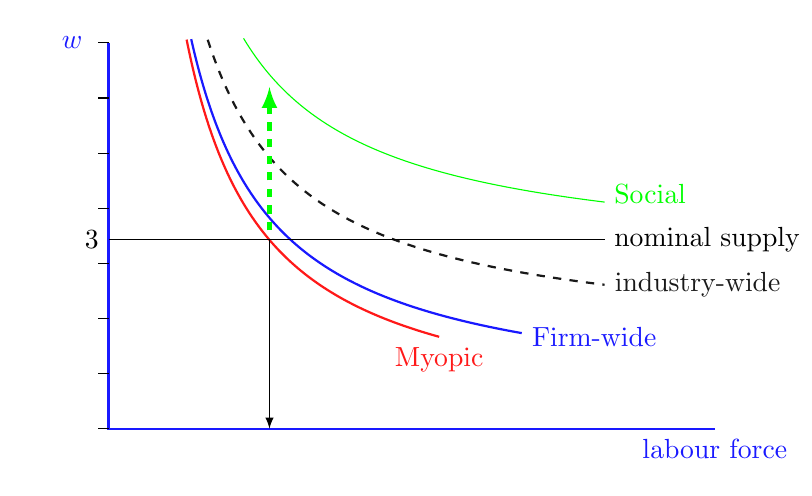
\begin{tikzpicture}[scale=.7]
%\def\bndmax{5}        %https://tex.stackexchange.com/questions/68462/filling-a-complex-region-with-tikz
%\def\bndmin{0.2}
\def \Y {7}  % height of y axis pecent
\def \W {15}  % length  of x axis
\def \Wbar {3} % jmeam wealth
\def \omega {3}
\def \A {1}  %was .5
\def \B {.5}

\draw [thick, color=blue!90] (0,\Y)node[left=.2cm]{$w$} -- (0,0)--(\W-4,0)node[below]{labour force};  
 \foreach \yi in {0,...,\Y} \draw (0,\yi)--(-.2,\yi)node[left]{};
 
\tikzset{func/.style={thick,  color=blue!90}}
% \draw[ func, domain=.2:\W-6] plot [samples=200] (\x, 2*\x^.5)node[below=.1, right]{SUPPLY};

\tikzset{func/.style={  color=green}}	
\draw[func, domain=2.45:\W-6] plot [samples=200] (\x, 10/\x+3)node[above=.1, right]{Social};

\tikzset{func/.style={thick, dashed, color=black!90}}	
\draw[func,domain=1.8:\W-6] plot [samples=200] (\x, 10/\x+1.5)node[ right]{industry-wide };

\tikzset{func/.style={thick, color=blue!90}}	
\draw[func,domain=1.5:\W-7.5] plot [samples=200] (\x, 10/\x+.4)node[below=.05, right]{Firm-wide};

\tikzset{func/.style={thick,color=red!90}}	
\draw[func,domain=8.5/6:\W-9] plot [samples=200] (\x, 10/\x)node[below]{Myopic};

\draw[](0,3.425)node[left]{$\omega$}--(9,3.425)node[right]{nominal supply };
\draw[thin,latex-](2.92,0)--(2.92,3.425); %a vertical labour supply
\draw[ultra thick,dashed, green,-latex](2.92,3.6)--(2.92,6.2);
%\draw [blue,  thick](13, 8.3)--(15,8.3)node [right, black] {\small A=\ 1,\ B=0.5};
%\draw [green, thick](13, 7.6)--(15,7.6)node [right, black] {\small A=.8, B=0.8};

%\node at (5,-1.5){Resulting in  profits, expansion, and/or entry: the city grows};
 \end{tikzpicture}
\caption{Multiple marginal products.}
\label{fig-marginal-products}
\end{figure}



Figure~\ref{fig-marginal-products} illustrates the problem. We can  make a distinction between the myopic marginal productivity curve observed by at the shop floor level and  the firm-wide effect of adding a worker. The red curve labeled ``Myopic'' represents the declining direct marginal productivity of labour as in might be observed by a shop manager, who could report how much more output one with one worker one lathe would produce. The blue line above it labeled ``Firm-wide'' represents the actual effect on firm productivity that arises because the new worker makes other workers in the firm more productive. This addition to output would be observable for managers reviewing the firm's performance over time. ' 

We can go on to consider the slower and distributed effect on closely related firms, which would raise any estimate of marginal product.  If there are 10 other firms and a new worker  has a small spillover effect  $\epsilon$ on each,  the spillovers raise the industry  marginal product  by $10\epsilon$. Each of the  10 other firms  enjoys  an additional $10\epsilon$ gain in the marginal product of their workers. This should lead to additional hiring by other firms.

Finally, expanding our view another step, we notice that if each of the  10 other firms hires one worker who produces an additional  $10\epsilon$ gain in output for all firms, the total spillover effect would rise by $100\epsilon$. The social marginal product of a single hire is indicated by the green line. 



\section{The system of cities}
Modern cities are not lonely and autarkic  beasts wandering their own exclusive territory and unconnected to others of the species. They are one is a global system of cities that compete and complement each other. Information, capital and even labour flows between cities are large. Henderson Abdel-Rahman\cite{Henderson1972Sizes}, Abdel-Rahman \cite{abdel-rahmanAgglomerationEconomiesTypes1990}, Fujita \cite{fujitaMonopolisticCompetitionModel1988}, Fujita, Krugman, and Venables \cite{fujitaSpatialEconomyCities1999}, and Fujita and Thiess \cite{fujitaEconomicsAgglomeration1996} among others provide models for expandingh the model in this direction.



\subsection{Taxes, municipal government, public goods, and productivity,}
This is a major issue with considerable development in the economics literature. Property taxes reduce the net locational value that flows to an individual owner but provides services and wages that make the city attractive. 

(create a regime where particular groups have an advantage)

Localized tax advantages can move a share of financialised investment into private consolidation of land.
including the structure of taxes for investment properties, institutional investors, individuals, etc.




\section{TO  METHODOLOGY?: Distribution}% not the right word
ABMs can be run multiple times to produce distributions of expected outcomes, which makes them valuable in planning exercises. They also do not require that we use a representative agent to make them tractable. Our model is intended to be elaborated  for such use. 

extensions
what it is
why it would be great to model
why it doesn't matter for our core results

\section{A possible typology of models and experiments}
While there  are many variations on the basic urban model and many potential experiments with each model there are only a few of immediate interest if the goal is to text the ``resilience'' of equilibria.

These models may exhibit irreversibilities in variables such as distribution, homelessness, city form, and class structure. 

The basic strategy for examining the system resilience is to shock a model (experiment) and then see if diagnostic variables recover. (This needs more precise expression.)

The first task is to select a subset of models an experiments that are of particular interests with respect to.

The second is to construct a model that allows those case to be examined. Ideally the model would be easily adapted to other experiments.

The following is a an attempt to develop a typology with a clear progressive structure.

Feedback - wealth allows upgrading. This advantages the rich. Maybe this 

\subsection{Models}
\begin{enumerate}
\item \textbf{A: The basic model}

The workhorse of urban economics is the circular city model. Some feature of the central place generates rents. It may be that it is the only employment centre. It may be economies of scale to a single activity or synergies arising from various externalities\footnote{We are interested in agglomeration economies. The wage  structure would then be related to the population or industry  structure. Externalities driving agglomeration may be classified  into two types, the  or so-called ``Marshalian''  and ``Jacobs'' externalities.}. 

In the simplest model, the central place pays a uniform wage, $w$ to all employees, who have identical preferences and transportation costs. $w$ is an attribute of individual residents. Residents  purchase or rent equal quantities of land at differing locations $l$ for identical housing.  

There are transportation costs $T$ that depend on distance from the  central place, so land close to the central place is more attractive than land farther from the central place.  

The equilibrium concept is that a market with identical individuals with identical incomes and transportation costs will result in identical utilities. The result is that land rent must decline with distance from the central place to offset rising transportation cost. 

The size of the city is determined by population and lot size. Income and transportation costs will interact with lot size. The basic model can be initialized by matching the number of properties to the size of the population. 

If population exceeds the number of properties there are three margins to consider
	\begin{enumerate}
		\item The land supply can increase. There may be a conversion cost
		\item The land per-capita may decrease. This is not simple in a city with land-use regulations, zoning, and fixed capital in homes. A conversion process has to be defined
		\item A homeless population can emerge. 
	\end{enumerate}

It is convenient in this model to use a \gls{Cobb-Douglas} utility function that has the property that a fixed fraction of income is spent on housing.  We can start with the assumption that earnings are fixed for the lifetime at the one-period wage, $w$. Then total spending on housing is $\beta Y, \beta <1$ and $ Y=w$. Let the transportation cost for a specific location $l$ be $T(l)$. The  equilibrium price at that location will be $P(l)= \beta Y-T(l)$.

It is convenient but not necessary to assume that land outside of the residential limit is costless. It is common to assume a fixed price for agricultural land. 

There is no fixed boundary and the size of the city is determined by the utility that can be achieved in competing regions of competing

\item \textbf{Y: The basic model with Income Differences}
This will result in segregation by neighbourhood depending on income. 

Income can be purely earning, which requires a distribution of $w$ across agents. Income  might include investment income, which  a private rate of return and a distribution of assets across agents. \footnote{A more subtle model could allow individual wages to be linked to the agglomeration of other workers - say engineers. we can imagine a city that has centres of agglomeration by profession or by complementarity. Depending on the production function, this should emerge endogenously.}
\footnote{Sufficient investment income could lead individuals to locate in cheap properties at the edge of the city.  Income might also be invested in property affecting the quality of a unit. This would require incorporating unit quality in the attribute list for each property, and introducing a quality preference  in the attribute s of residents.}

\item \textbf{L: The basic model with Locational Preferences}
This will result in segregation by neighbourhood depending on preferences.

One version would be include distance to the edge of the city as an amenity in the utility function. Another would be to locate amenities within the city. These would lead to higher prices near amenities.

A natural variant would be to have earning depend on location. If there were several locations  a polycentric city would emerge.

\item \textbf{T: The basic model with varied transportation cost }
This will result in segregation by neighbourhood depending on income and Transportation costs. Experiments include cars for the rich and  transit. 

Diagnostics include change in total transportation cost and differential welfare effects.

\item \textbf{R: The basic model with a rent-own choice}
This may result in the emergence of classes. Agents must have the capacity to borrow to purchase. Attributes of the agents and must now include  net assets,  an available interest rate, and a permissible mortgage.

We imagine a banker setting the mortgage rates and size. This can be done at the beginning of each period for each agent. 

With no income differential we expect equal utiliites

\item \textbf{YR: The basic model with earnings (Y) differences and a rent-own choice}
This model is likely to generate diverging classes as income differentials permit some to capture land rents from others. This is highly likely if borrowing costs decline with income and asset ownership.

\item \textbf{L: The basic model with variable lot size}
This is achieved by making lot size a choice variable for households, in which case we will get a trade off between transportation cost and lot size and distance. Results for this model are known. Density  falls with distance from the centre. 

\item \textbf{YL: The basic model with earnings (Y) differences and variable lot size}
The wealthy choose larger homes and lots farther form the centre

\item \textbf{S: The basic model with constant lot size and variable density}
This is achieved by allowing stacking of housing units. Results for this model are not known. This introduces a step change in housing form, and emphasizes unit size.

This model should produce some interesting spatial patterns, especially if couples with the possibility of secondary central places.

\item \textbf{YS: The basic model with earnings (Y) differences, constant lot size and variable density}

This model should produce some interesting spatial patterns, especially if couples with the possibility of secondary central places.

\item \textbf{IR: The basic model with outside investors and rent-own}

\item \textbf{IYR: The basic model with outside investors, earnings differentials and rent-own choice} This model is of interest if borrowing costs decline with income and asset ownership.
\end{enumerate}
\subsection{Experiments}
There are various experiments of interest. You will have to pick key ones. It is not necessary to do all of them in every model. 

	\begin{enumerate}
		\item increase population
		\item increase wage
		\item add hard boundary (limit land)
		\item Introduce differential incomes
		\item Introduce differential access to capital
	\end{enumerate}

% \newcommand{\cred}{\cellcolor{red!30}}
% \begin{table}[htp]
% \caption{Potential experiments: \textbf{Pick some}}
% \begin{center}
% \begin{tabular}{|c|c|c|c|c|c|}\hline

%   &\multicolumn{5}{c|} {experiments}\\ \cline{2-6}
% Model  &1 &2  & 4 &4  & \\ \hline
%  A& \cred& \cred  &  \cred & \cred  & \cred  \\
%  Y& \cred   & \cred   & \cred   &\cred    &\cred   \\
%  T & \cred   & \cred   & \cred   &\cred    &\cred   \\
%  R & etc &  &  &  & \\
%  L &  &  &  &  & \\
%  S&  &  &  &  & \\
%  I &  &  &  &  & \\
%  YR &  &  &  &  & \\
%  IR &  &  &  &  & \\
%   IYR&  &  &  &  & \\\hline
% \end{tabular}
% \end{center}
% \label{default}
% \end{table}%

\chapter{Future work to SORT}
model development (experiments and extensions)
interventions
theoretical development
% The urban production sector pays a wage premium $w$
%This is a convenient simplification, not a necessary feature of the model. 

The rental value of land shapes the city spatially.  

\section{Experiments with this model}
Lots of simple extensions e.g. 2 cities with immigration, differentiated labour, products, market power, neighbourhood effects (see extensions map/typology), we focus on those elements central to seeing the structure of the resilience dynamics of the wealth/housing effect. Consider adding density, to look at how it interacts with agglomeration effects. (integrating with transportation effects is neat)

\subsection{Initial state}
Basic experiments has all homes owner occupied to start. Other initial tenure mixtures are easily modelled. WHY WE MIGHT WANT TO

The basic model can be initialized by matching the number of properties to the size of the population. 

In the simplest version, firms concentrate at the city centre. Workers are spread over space and pay transportation costs to commute.

The size of the city is determined by population and lot size. Income and transportation costs will interact with lot size. 

\subsection{Parameter values}

\subsection{Analysis methods}
mapping of regimes

\subsection{Data}
incorporation of local data more carefully

\section{Extensions to the model}
The simple circular city can be extended to to produce other forms, including polycentric cities and hierarchies of cities at the cost of additional computational complexity. The simple case we examine will allows us to focus on the general, and neglected, distributional features of this class of models.

\subsection{Lags and adjustment processes}
The details of the adjustment process and the system lags are selected primarily for convenience in simulations. Real-time lags are important and complex, we explore some sensitivity results, but can explore more. 

We model a fairly short lag although in reality lags are long and variable. 

\subsection{Labour adjustment costs}

in the agent model, employees are simply laid off and seek work, so there is unemployment, but there are not \glspl{labour adjustment cost} for firms.

\subsection{Agglomeration effects, and returns to scale}
The case where there are increasing returns at the city level introduces interesting dynamics, explored in appendix CITE % 'furthur discussion' appendix.

We incorporate agglomeration effects using a Cobb Douglas formulation. This allows us to focus on the results of agglomeration in the urban system, rather than specifying the system of firms that transmit the effect. 
There are a number of other ways to study the aglomeration process in more or less explicit ways.

MOVE TO PARAMETER VALUE DISCUSSION?
The strength of the agglomeration is given by $\gamma$, thus for $\gamma=0$ there are not agglomeration effects. APPENDIX?
By definition, with one person, the agglomeration effect has no influence, $\Lambda(1)=1$,  as in the \gls{Cobb-Douglas}, and empirical urban scaling results tell us that agglomeration increases with population, following a power law distribution, so we know %$\die
FIX EQN ERROR die ${\Lambda}{n}>0$. 
%%%%%%%%%. ***WHY
If $\beta=1-\alpha$, this is a \gls{constant returns to scale} production function. Without agglomeration effects, $T(n)=1$,  Then  \textbf{$\mathbf{L(n) = T(n) n}$}  WHAT IS T, WHAT IS THIS TELLING US?
Without agglomeration effects, $\Lambda(n)=1$,  Then  \textbf{$\mathbf{L(n) = T(n) n}$} 


\subsection{Returns to scale and firm under-investment}
Each firm has \gls{decreasing returns to scale}, which means each new worker increases output by less than the previous worker did.
RETURNS TO FIRM CAN BE DECLINING WHILE RETURNS TO CITY INCREASING, THEN FIRM UNDER INVESTS
explore this in the model, see Equation~\ref{eqn-prod1}.

\begin{equation}
Y=K_i^{\alpha }(\Lambda(n)n_i)^{\beta }.
% \label{eqn-prod1}
\end{equation}

MOVE DISCUSSION HERE FOR NOW

\subsection{Heterogeneous agents}
In the simplest model, the central place pays a uniform wage premium, $w$ to all employees, who have identical preferences and transportation costs. 
The wage $w$ is an attribute of individual residents.  
It is straightforward to vary i and to vary preferences. 

relax assumptions and look at how the interaction between the production of social wealth in cities interacts with housing and the extraction of rent to drive patterns in a richer model with heterogenous agents interacting over space and time. 

- wages, skill sets

\subsection{Forward looking agents}
There are reasons to expect the results obtained with  forward-looking agents to differ substantially from those obtained with a model featuring myopic agents.\footnote{For example, Lecca et al. *** \cite{LOST-Lecca-et-al-2013}  used a stylized computational macroeconomic model applicable to a regional context to demonstrate that the assumption of myopic vs forward-looking agents yields differences in the dynamics generated by a shock perturbing the initial steady state, even though the alternative paths lead to the same long-run equilibrium.} 

\subsection{Rental bidding process}
 "Just as with prices, there is an economically \gls{warranted rent} which may differ from the \gls{market rent}. Individuals make their investment decisions on their own expectations rents. the bidding process on rental properties is abstracted in the base model. Instead of modelling the process explicitly, we make the assumption that the warranted rent is the market rent, $\mathcal{R}_W = \mathcal{R}_M$." .. could implement

\subsection{Amenity}
Notation for amenity.
There may be a band surrounding the city or persons who do not commute but enjoy urban consumption amenities. 
based on location etc

\subsection{Preferences}
A utility function/algorithm specifies agents preferences over the attributes that matter. - algorithmic continuous. lexicographic- any traits. 

\subsection{Unemployment and labour adjustment costs}
There is no unemployment. there are no labour adjustment costs for firms. ***INTERESTING TO THINK ABOUT  
when people would stop working with

 falls to subsistence wage -
 too much rent, I guess they leave, they can always move somewhere

\subsection{Moving costs}
     If there are moving costs, people can be trapped in a bad situation, incurring debt, and it can still be not worthwhile to move

\subsection{Mobility}
We could look at mobility in a more sophisticated way..
Agents enter the urban market two ways. If wages rise, agents just outside the city may become commuters. This increases population. 

When homeowners in the city retire they sell their home and move to the country. This allows them  to enjoy the capital value of their home.  They either sell their home or rent it to a new occupant. 

When  tenants in the city retire they would move to the country to enjoy lower rents. This has no effect on population. It is simplest, therefore to treat tenants as permanent residents unless we want the tenant's retirement to trigger an event like a rent increase or a decision by the owner to sell the property.

\subsection{Transportation costs}
Wage and transportation cost determine the radius of the circular city, which determines the size of the labour force which affects urban productivity. The cost of travel is therefore an important variable in the development of urban productivity. 

the transportation cost/distance relationship appears to be non-linear in many cases. While the linear model connects with the established literature, we likely want to explore the implications of more empirically grounded curve (e.g. \cite{bertaudSpatialDistributionPopulation2003}).

\subsection{Multiple firms and production structure}
The scaling result at the level of the city allows us to incorporate the effect of agglomeration in a standard \gls{circular city} model in a simple way. 

We could also explicitly model labour markets and competing firms. 

Explicitly modelling labour markets with multiple firms is a natural way to specify the model more completely, see Appendix~\ref{appendix-future-work},  but it would require introducing many ancillary assumptions and selecting among alternative models of agglomeration, when when we want to focus on distributional and growth-affecting features of the system.

For simplicity, assume firms produce a variety of perfectly substitutable commodities which are exported and locally consumed at a fixed price in a large market. 
***  Increasing product variety may produce a consumption agglomeration economies as in \cite{fujitaSpatialEconomyCities1999}.

\subsection{Market power and interchangeable goods - local markets etc}
MAKE A FOOTNOTE ON MARKET POWER AND INTERCHANGIBLE GOODS??
No externalities imperfect information etc.. ensure efficiency but aren't needed, all you need is price taking for individuals to only pay attention to their own costs and their own benefits. 

\gls{externalities}, \gls{imperfect information}, \gls{monopsony}, \gls{duopoly}, \gls{monopoly}

competitive markets many sellers, many buyers, monopoly single seller, monopsony - single buyer, intermediate cases - monopolistic competition - with some market power but not complete - duopoly- some inefficiency depending on the behavioural model because in the duopoly case they may be able to take advantage of the behaviour of buyers.

Start with perfect competition, then introduce monopolistic competition is most likely.. but it's more difficult to handle. e.g. with brand names, people have some preference for some feature of your particular good so you can price it higher even though you may loose some marginal people. Firms compete on brand name and reputation, not the pure cost effect.

In the spatial economy, goods are deferentially interchangeable. Put them on a line and firms pick a place along they line. Firms are in competition but are competing on a line-.. spatial model moved over to characteristic space..---looking at this would involve overlaying another space - the characteristic space on the physical space. .. There are also local places with local grocery stores. Polycentric stores have effectively monopolistic competition in real space. - like a named cafe downtown has the same.

\subsection{Sectors}
..


\subsection{Incomes}
In the model receive the\gls{urban wage}, which is the subsistence wage plus the urban wage premium $\psi + w$.

They may get different incomes because of firm, sector or individual increases, or particularities of the 
hiring/negotiation/wadge adjustment process, path dependency, stochasticity, etc. 
All of these factors could be explored formally in the model. %ref{rockefeller}


POOR STRUCTURALLY DISADVANTAGED HOWEVER RICH WE GET
these are averages-- some are structurally below average so some are always behind simply because of the structure of the rents claimed.. that's built in FUTURE WORK- DIFFERENT INCOMES GETS YOU THAT. 



\subsection{Hiring process and unemployment} \label{section-rockefeller}
 In our model, non-urban landowners are those who live too far from the urban job center to justify commuting.  Agents join the urban market by adding their names to the firm's list of job applicants when the rent on the marginal unit of land exceeds the transportation cost. 

adjustment speeds..
 
i(did extended modelling in the Rockefeller social innovation lab)- barriers of employment for young people seeking work
- prison records, transportation, family responsibility, bias, educational attainment, expectations of success, neighbourhood factors etc.
Could explore that kind of structure in this model

\subsection{Demographics}
Could build a population model suited to particualr data sets %\ref{section-rockefeller}

\subsection{Skills and individual productivity}
The basic model consideres a non-differentiated workforce. We can add particular skills.
Some agents can be more productive than one another

Agents may move to cities to assemble networks (model as networks)
and learn specialized skills

It can evolve over time so agents can productively over pay to  
-- getting debt/resources at key stages in a persons development to aquire property and skills is important to \gls{wealth trajectories}


\subsection{Sources of agglomeration effects}
Some of the empirically wage difference comes from the dense resources  - location of cities in good places, public investment- libraries - institutions, the network effects
some from the ability of those close to the center to simply claim a larger share of resources
some 
Some of the agglomeration wage may come from people with resources and skills disproportionately choosing cities for their amenity effect. 

We can explore different drivers in the model.


\subsection{TO METHODOLOGY: Rural market and other cities}

 To simplify analysis, we assume that land outside of the residential limit is costless, following th common practice of assuming a fixed price for agricultural land \cite{GET_fixed-price-ag-land}. 

The model is constructed so that there is neither land rent nor capitalist exploitation in the rural economy. 
This special case allows us to examine the distribution of the social surplus generated by agglomeration economies and the effect of financialization.

We could explore this

\section{Interventions: Policy and Agent Strategies}
Extended appropriately, this basic model could be used for planning.

detailed models of interventions typologies of interventions e.g. local currencies, decaying currencies, 

\subsubsection{Teaching}
could use for teaching a sequence for illustration could follow to introduce x ideas - see above. - rent, space, finance treated separately, - tool to think about their relation

productivity centered urban and spatial policy

connects with growth, economic development in real places work

\subsection{Zoning}
zoning - layers interact

\subsection{Taxes}
property taxes reduce the net locational value that flows to an owner but provides services and wages that make the city attractive. 

(create a regime where particular groups have an advantage)

Localized tax advantages can move a share of financilized investment into private consolidation of land.
including structure of taxes for investment properties, institutional investors, individuals, etc.


\subsection{Insurance, risk, and mortgage backing}

Uncertainty is a key variable.

The effects of policy are large. For example in Canada, backing mortgages is the largest fiscal investment at the national level \cite{nemtinFinancializationHousingSocial2021}.

- risks, bubbles, collapse


\subsection{Housing quality, size, subdivision}
Residents  purchase or rent equal quantities of land at differing locations %$l$ 
for identical housing.  DOWN

? More generally, if we were to introduce variations in lot size and housing types  we would want the integral of the worker density function. In our ABM version  of the model we simply count the workers within the commuter shed.

\subsection{Development and Improvements}
The supply of land at any distance from the center is inelastic. 
Its value comes from proximity to the productive urban centre, not from the value of improvements made to the property.

*** Without density, the labour supply increases with the square of the wage.  other forms..

- We have an empirical curve - gives density- simply build in

- We can .. Model a subdivision process-- urban SIM, a collaborator on the missing middle grant. - model of pro-forma and typoloties/ policies makes it possible to follow..

Some nonlinearities e.g. Some may buy land seeking to develop property in the future and let it become run down. 

We could add improvements
 or consolidation, subdivision, and development. 

% Reference sections on development which is different, and the contribution of amenity % Because supply is fixed for urban land, and the landowner has a monopoly claim on rents, the rents that can be depend on wages and amenity rather than the cost of improvements made to the property.
% The source of rents is the free gifts of nature, the coming together of people to create value in cities, and the concentration of public amenity in cities. 

\section{Theory - how to pay for innovation?}

Leaving land out, however, creates a problem in  the neoclassical growth theories we will examine below. John B. Davis \cite{davisRicardoTheoryProfit1993} noted that ``Questions arise, however, when one turns to exchange between a sector paying rent and one not.'' 
Under the assumption of perfectly competitive goods and factors markets as well as marginal productivity pricing of capital and labour, neoclassical growth requires technical change to be generated outside the model because there are no resources left to innovate if both factors of production are paid their marginal product.\footnote{This follows from Euler's theorem: if, for a given level of technology $\bar A$ output Y is produced according to a \textbf{constant returns to scale} and twice continuously differentiable function of capital and labour $F(K, L, \bar A)$, Euler's theorem implies that $F_K K + F_L L=Y$, where $F_i$ is the marginal product of factor $i$. Payments to  capital and labour take up the entire national product and no resources are left to finance the production of technology-improving innovations. are paid their marginal product.} 
If, however, land is reintroduced, as it must be in an urban model, there must be rents and there is therefore a surplus available for innovation.
\footnote{An alternative and common approach is to assume imperfect competition, which may be based on increasing returns to scale, in which case firms with market power may achieve a surplus. ``Although seldom modeled outside the monopolistic competition framework, market incompleteness and imperfect competition are central to the new growth theories'' (Gilles Duranton, Growth and imperfect competition on factor markets: Increasing returns and distribution, European Economic Review, 44-2, 2000, 255-280), Similarly, Sjak Smulders and Theo van de Klundert conclude that ``Growth is higher in a more concentrated market provided that market power of firms is not too high,'' (Imperfect competition, concentration and growth with firm-specific R \& D, European Economic Review, 39-1, 1995,139-160).}



\section{SORT Rough Notes}
what does a speculative over investment.  in housing  do? - hollowed out store front

who carries what risks- banks vs individuals

subdivision and density

multiple cities,
linear cities

differential skills and wages,
work from home

details of typologies, transportation networks, etc

- make it available as a part for other models, use other models in this model


 

\subsection{Implications}
\subsubsection{Agglomeration driven under-investment}

% % \chapter[Model Implementation]{Model Implementation}
\label{appendix-model-implementation}

\section{Urban wage premium}

$\omega$ is the urban wage premium. It is a share of the urban agglomeration effect. 

I think of this as worker income, $\psi + \omega + r_prime*savings$ 

The wage income  $\psi + \omega$ part has to be related to the marginal productivity of workers. The urban output function from Lobo et al \cite{loboUrbanScalingProduction2013} is  
\begin{equation}Y=AN^\beta\label{LoboEqn2}\end{equation}

Where $\beta$  is the scaling exponent, with a value of,  for example, 1.13  \`a la 
Lobo. $A$ is called the ``scale factor.''\footnote{Much of the analysis assumes scale invariance of  $A$.}  The \textbf{total urban marginal productivity of a worker} is  
\[UMPL=\beta AN^{\beta-1}=\frac{\beta Y}{N} =\]
This is not the same as the \textbf{firm-level marginal productivity of a worker}. The worker total share in Lobo et al. is \[W= (1-\alpha)Y \] 
so the individual share, which should be the competitive wage, is
\[W= \frac{(1-\alpha)Y}{N} \] 
where $(1-\alpha)=0.8$ is a common estimate. If we assume that this sets the rural wage,$\phi$, then $\omega$ has to come out of the  urban surplus per worker,

\[surp= \frac{\beta -(1-\alpha)Y}{N} \] 

 so set a fraction $\lambda$ of the surplus a, and 
 \[\omega= \lambda\frac{\beta -(1-\alpha)Y}{N}= (1.13-.8) \frac{Y}{N} \] 

 Since capital expects 0.2 as its payment and labor 0.8, the surplus available to share has to be taken out of the 0.13. The easiest formulation then is probably 
 \[\omega= \lambda(\beta -1) \frac{Y}{N} =\lambda(\beta -1) \frac{AN^\beta}{N} \] 
 

$(\beta -1)$ is agglom and  $\lambda(\beta -1)$ is the workers' share of the surplus over and above the \gls{constant returns to scale} (CRS) case.   $\lambda(\beta -1)$ is 

\begin{lstlisting}
# Firm step function updates wage, omega
def step(self):
    prefactor  = self.model.prefactor
    agglom     = self.model.agglomeration_ratio
    population = self.model.agglomeration_population
    wage_share = self.model.wage_share  
    wage_premium = wage_share * (agglom-1) * prefactor * population**agglom # omega
    self.wage = wage_premium + self.model.psi
    # k thought # self.wage_premium = (wage_share * prefactor * population**agglom)/ population # omega    
    # note surplus is: (beta - 1) * (prefactor * population**agglom)
\end{lstlisting}

Where wage share is a parameter input to the model.

\section{Bidding}
\subsection{Subjective discounting}
\begin{lstlisting}
def get_discounting(self):
    """
    Delta is the subjective individual discount factor for agent
    after one year. This will be close to ri
    A factor may be a compounded rate.
    It is the present value of one dollar in one year 
    Turns one dollar in one period into dollars of present value.
    sum_delta is sum of the infinite series 
    minus discounted infinite series after mortgage_period years
    It is the present value of annual payments from one to 
    mortgage_period years e.g. of mortgage payments or rent received
    delta_mortgage_period was called   delta_period_T
    """
    
    delta = self.r_prime # if constant 
    delta_period_1 = 1 / (1 + delta) 
    delta_mortgage_period = delta_period_1**self.mortgage_period
    sum_delta = delta_mortgage_period * (1 - delta_mortgage_period)
    # Note delta_mortgage_period is subtracted to subtract the long tail
    return sum_delta
\end{lstlisting}

Delta could also depend on wealth. For example,  use the bank rate, which is the rational rate but people who are poor typically have higher rates.  It would not change as the central bank changes r-pirme
% delta could be wealth based typically higher for poor.

\begin{lstlisting}
# A version with delta depending on wealth
wealth = self.wealth
delta =
\end{lstlisting}
 
\subsection{Maintenance costs}
\begin{lstlisting}
    def get_maintenance(self):
        """Maintenance share of property service (a*b*psi summed and discounted)
        OR IS IT TOTAL maintenance COST OVER THE MORTGAGE PERIOD?
        """
        a   = self.housing_services_share
        b   = self.maintenance_share
        psi = self.subsistence_wage
        sum_delta = self.sum_delta # CALCULATE PER PERSON
        return (a * b * psi) * sum_delta
\end{lstlisting}

\subsection{Taxes}
\begin{lstlisting}
    def get_tax(self):
        """ 
        THIS DOES NOT CHANGE WITH INCREASING WAGES?
        BUT THAT IS THE MAIN WAY TO FUND A CITY

        WHAT TO CALL THIS WEHRE DOES IT GO. WHERE DO WE USE THIS VS TAU
        Just for initialization? - warranted price. 
        Use warranted prices as initialization
        Tax costs for the mortgage period, T. 
        (Example of rate for an  multiperiod annual rate)
        tax_T= tau*(omega-c*d + a*psi) * sum_delta_T
        This is assuming taxes are paid at the end of each year for T years
        tau_T       = tau * sum_T_delta 
        #  present value of the tax rate over T years        
        """
        tau   = self.model.property_tax_annually
        omega = self.firm.wage_premium # FIXED
        psi   = self.model.subsistence_wage
        a     = self.model.housing_services_share
        c     = self.model.transport_cost_per_dist # RENAME
        d     = self.distance_from_center
        sum_delta = self.model.sum_delta # TODO - make individual  - this would have to be average discounting - THIS TAKE SUM DELTA OUT - AND PUT WITH LARGER CALCULATION.. - CACLULATE FOR A PERSON/PROPERTY COMBINATION..
        return tau * (omega - c*d + a*psi) * sum_delta
\end{lstlisting}


\subsection{TODO Warranted price}
\begin{lstlisting}
@property
def warranted_price(self):
    # USELESS PLACEHOLDER - GET CALCULATION
    return self.model.firm.wage/(self.transport_cost + 1) 
\end{lstlisting}

\subsection{TODO Maximum mortgage calculation}

\textbf{wealth-based  mortgage maximum} 
 \[max\ m_i = 9-\left(\frac{W_i}{\bar W}\right)^{0.1} \]

% **Source**: Ch:model line 580, page 87.. I have done some fiddling Wealth $W_i = P-M+S.  for i - real estate agents estimated price wealth of a property owner as assessed by the bank

\textbf{income-based  mortgage maximum} of 

\[M^{max}_Yi = \frac{0.28*(\omega+w)}{r_i}\] It is the maximum the bank will let you pay.

\textbf{Combined  mortgage maximum}
\[ M_i^Y{max} = min \{9-\left(\frac{W_i}{\bar W}\right)^{0.1}P,  \frac{0.28*(\omega+w)}{r_i} \}\]

\begin{lstlisting}
# Max mortgage
wealth = property_value - mortgage + savings
mean_weath = sum(wealth)/number_of_people

def get_max_mortgage(self, applicant):
    max_mortgage =  ...
    
    return max_mortgage
\end{lstlisting}

% wealth = property_value + 
wealth $W_i = P_e-M+S$.  

- Also need mean wealth. $\bar W$ , which you have to calculate from the sums for property values total mortgages issued, and individual savings. The bank could keep these values
- Individual borrowing rate 
$r_i = (A + B \frac{\bar{W}}{W_i})\bar r=(.1 + B \frac{\bar{W}}{W_i})\bar r$.
The value .1 can be seen as the bank's share of the prime rate set by the Bank of Canada. this is an easy place to insert that value. We should discuss this detail. An alternative is
$r_i = (0 + B \frac{\bar{W}}{W_i})(\bar r_i+ bank\ margin)$.

- Maximum M  from wealth constraint = $(9-(W_i/\bar W)^{0.1}P$
  Check if $(W_i/\bar W)0.9P$ will work. 
- Maximum M  from income = $M^{max}_Yi = \frac{0.28*(\omega+w)}{r_i}$ 
% - Maximum M  $M= min(0.28*(omega+phi)/r_i,  0.8P$,  (9-(W_i/\bar W)^{0.1}P,  \frac{0.28*(\omega+w)}{r_i}   } $


 
\subsection{Net rent based on}
Tenant willing to pay, vs what it is worth for a company to buy a property.

\begin{lstlisting}
def get_net_rent(self, property):
    """Compute the rent for a land parcel, or what someone could afford
    to pay to live there. 

    Rent depends on the urban wage premium over and above the subsistence
    wage, and on transportation costs and the distance to the
    central business district. Applies with a single wage. Adjust for
    differential urban wages.

    :param property: the land parcel to get rent information for.
    """
    a     = self.model.housing_services_share
    b     = self.model.maintenance_share
    c     = self.model.transport_cost_per_dist # RENAME
    d     = property.distance_from_center 
    tau   = self.model.property_tax_annually 
    # property_tax_rate # IS THIS FOR THE MORTGAGE PERIOD
    psi   = self.model.subsistence_wage
    omega = self.model.workers_share
    return omega - c*d - a*psi - b*a*psi - tau*a*psi
    # urban_wage = self.model.firm.wage
\end{lstlisting}


\subsection{Net rent based on ..}

\begin{lstlisting}
def get_net_rent(self, property):
    """Compute the rent for a land parcel, or what someone could afford
    to pay to live there. 

    Rent depends on the urban wage premium over and above the subsistence
    wage, and on transportation costs and the distance to the
    central business district. Applies with a single wage. Adjust for
    differential urban wages.

    :param property: the land parcel to get rent information for.
    """
    a     = self.model.housing_services_share
    b     = self.model.maintenance_share
    c     = self.model.transport_cost_per_dist # RENAME
    d     = property.distance_from_center 
    tau   = self.model.property_tax_annually 
    # property_tax_rate # IS THIS FOR THE MORTGAGE PERIOD
    psi   = self.model.subsistence_wage
    omega = self.model.workers_share
    return omega - c*d - a*psi - b*a*psi - tau*a*psi
    # urban_wage = self.model.firm.wage
\end{lstlisting}

\subsection{Max Bid}

Calculate max desired bid for an agent
\begin{lstlisting}
    def get_max_bid(self, property, bidder):
        net_rent = self.get_net_rent(property)
        r        = self.model.r_prime   
        r_target = r + self.model.r_premium
        m        = 0.8 # TODO FIX - ADD WEALTH
        # I can't do delta_T. It reads as delta_transpose to me.
        sum_delta    = self.model.sum_delta 
        p_dot    = 0.01 # TODO - estimate rate of price change
        return net_rent/((1 - m)*r_target - sum_delta*(1 + p_dot - (1 + r)*m))
\end{lstlisting}

Agent will bid the min of the desired bid or the max allowed mortgage
\begin{lstlisting}
max_mortgage = self.bank.get_max_mortgage(self)
min_downpayment = self.bank.min_down_payment_share * max_mortgage
downpayment = min(min_downpayment, self.savings)
max_allowed_bid = max_mortgage + downpayment
for sale_property in (self.model.realtor.sale_listing):
    # max_bid = self.bank.get_max_bid(sale_property, self)
    # TODO Fix
    max_desired_bid = self.model.bank.get_max_bid(sale_property, self)
    max_bid = min(max_allowed_bid, max_desired_bid)
\end{lstlisting}

\section{Negotiation Process}

Bidding.

There is a problem in that they bid on all properties as a short cut. If the number of bids structures the negotiation process, we need to limit their bids or do something much more iterative. (see above section)




\section{Individual Accounting}

\begin{lstlisting}
# FIX - NEED TO ADD THIS
# Update savings
self.savings += self.model.savings_per_step

# TODO pay costs for any properties owned
# if self.residence in self.properties_owned:
#     # TODO pay mortgage if needed pay costs
#     pass
# else:
#     self.savings -= self.rent # TODO check this is right rent
\end{lstlisting}
% % \chapter[Parameters]{Computing Bid Price Parameters}
\label{AppendixParemeters}

% \section{Relating the bid price parameters to the code}
The bid price is: 
\begin{align}
P^{bid} \ge   \frac{ \mathcal{R}_N}{(1-m)r^{target}-\left[ \delta(1+L(P)- (1+r)m)\right]}. \nonumber
\end{align}
In the following sections, we discuss each of the terms and how they are implemented in the code. Sections are numbered: 
\begin{align}
\frac{\ref{SS:NetRent}} {(1-\ref{SS:BorrowingRatio})\ref{SS:targetr}-
\left[ \ref{SS:discountfactor}(1+\ref{SS:PriceForecast}- (1+\ref{SS:BankRate})\ref{SS:YWealthConstraint})\right]} \nonumber
\end{align}

\section{Net rent}\label{SS:NetRent}

$\mathcal{R}_N = \phi \mathcal{R}$


Where the \gls{rent share}, phi is a fraction
$\phi = (rent-taxes-costs) /rent$ 

There's a distinction between the warranted rent, the net rent, and the rent that's actually charged.



We assume that the  rent  actually charged to a tenant is the warranted economic rent, ($\mathcal{R}= \omega - \tau d_j$), but the relevant term to enter into the calculation of return on investment is the net rent $\mathcal{R}_N$ for a given property, because the returns are the returns an investor can get after paying taxes and operating costs.

In our computational model, we do the calculation in terms of a mortgage, so we want the total returns after expenses, in present value, compounded over the mortgage  period.
% We want the total returns after expenses, in present value, compounded over a 5 year period.


\begin{align}
\mathcal{R}_N &= \mathcal{R} - \Theta - \Sigma 
\end{align}


In terms of the warranted rent, 
\begin{align}
\mathcal{R}_N &= (1-\kappa_j - \sigma_j)(\omega - \tau d_j)
\end{align}

% $\mathcal{R}_N = (1-\kappa_j - \sigma_j) (\omega - \tau d_j)$

% {\color{red}
% Notice that  we need here is really the fraction of the warranted rent that the owner gets to keep after maintenance costs and taxes. It is possible that the owner is charging more or less than the economic  rent, but economic rent can be seen as an equilibrium value. Economic rent is $\mathcal{R}$.  This is (tautologically) related to the price as a fraction of the actual sale price: COULD MOVE TO THE CHAPTER NOW SINCE THE THE SECTION IS MOVED THER
% }

% \[\mathcal{R}= \frac{\mathcal{R}}{P_0}P_0 \]



If we want to know the  present value  of the \textbf{net rent}, $\mathcal{R}_N$  collect over the period  $T$, $\mathcal{R}_N^T$, we \textbf{add up} the discounted rents for each year. We may assume the rents are rising at and that the first is the current warranted rent, which gives us a computational formula. 
\[\mathcal{R}_N^T= (\omega-\tau*d)\sum_{t=0}^{t=T-1} \frac{(1+\dot{\mathcal{R}})^{t}} {(1+r_{r_\delta})^{t+1}} \]


% \[\mathcal{R}_Nj^T= (\omega-\tau*d_j)\sum_{\tau=0}^{\tau=T-1}\left[\frac{1+\dot{\mathcal{R}}}{1+r_{r_\delta}}\right]^\tau \]
\noindent where $\dot{\mathcal{R}}$ is an expected rate of change of rents - possibly zero for now, and $r_\delta$ is the individual's discount rate. 

TODO: problem - how to handle subscripts with net rent $\mathcal{R}_N$



\subsection{Target interest rate}\label{SS:targetr}

 The target interest rate, $r^{target}$, is the prime rate plus a margin. % required by the bank.  Question: do non-bank actors have such a term?

\begin{verbatim}
self.get-target-interest-rate(buyer)
\end{verbatim}


\subsection{Tax ratio}\label{SS:taxratio} 
The tax ratio $\sigma$ is the share of rents that the municipality takes for services and infrastructure. This fraction of the value of the property is about 30\% based on mill rates in Ontario,  so $\sigma = 0.3$. % REFERENCE

*** CHECK Total taxes paid on  property $j$, over a given mortgage period $T$ is 

\[\Psi_j^T = \psi * \mathcal{R}\].  


\subsection{Cost tax ratio}\label{SS:costratio} 
The value of $\kappa$  varies for every property based on maintenance requirements, historic rents, tenant rights, and variations in assessed values. If it varies, it may be useful as a quality indicator.

%Values for $\kappa$ and $\sigma$ must be adjusted to take into account the length of the period or net rents have to be summed over the period.  NO LONGER NEEDED 

Nothing prevents $\sigma+\kappa >1$, which would leave an investor unable to cover building maintenance and taxes out of current rent. 


\subsection{Discount factor}\label{SS:discountfactor}

The discount factor $\delta_i$ for THE END OF period $T$ captures the cost of waiting $T$ periods to sell the property. The usual way to treat it, which we use here, is to assume that $i$ has an interest rate $r_i$ and has been investing efficiently. This means that  the individual has a discount factor for future returns based on the year-over-year rate of return. 

\[\delta^T_i=\left[\frac{1}{1+r_i}\right]^T\]


\subsection{Price forecast approximation} \label{SS:PriceForecast}
$L(p)$

$p$ is all the price data plus any exogenous information (EG Policy knowledge?). $L(p)$ is an estimation function that produces a `common knowledge' value for the rate of price increase. Later you can add idiosyncratic extra knowledge or extra ignorance.




\subsection{Prime interest rate}\label{SS:BankRate}
$r$

The bank's interest rate, $r$, is just the bank rate (prime rate? set by the Bank of Canada. Exogenous. Just assign  a value like 4\%.


\subsection{Borrowing ratio}\label{SS:BorrowingRatio}
$m_i$

The borrowing ratio, $m_i$, is just the fraction of the price that the bank will lend to a potential buyer. \textbf{It may depend on the individual.} 

Income(\ref{SS:YWealthConstraint}) and/or wealth (\ref {SS:MWealthConstraint}) may constrain individual participation in markets. 
Here we should use the same logic as we use about the interest rate charged. (\ref{SS:BorowingRate})


It is likely to be higher for institutional buyers  and for rich people because the bank thinks rich people are more secure risks. they may have other assets that could be attached in the case of default.

\subsection{Wealth constraint on m} \label{SS:MWealthConstraint}


I have suggested that the availability of  capital is known to differ for rich and poor. 
The bank, as a person has lots of assets, so $m_i$ is close to one, say 0.9. 

For the median wealth holder, $m_i$ should be around - let's say, 0.8 and  
We need a function that captures this relationship so we need to define individual wealth:
\[W_i= P_i -M_i  +S_i\]
where 

\begin{tabular}{ll}
$P_i$ & value of owned home\\
$M_i$ & Mortgage on owned home\\
$S_i$ & personal savings = $age*d*W$\\
\end{tabular}


We first tie the borrowing \textbf{ratio}, $m_i$,  for agent $i$, to individual wealth. Figure~\ref{Fig:Borrowingratio} illustrates a mortgage availability  model that is written 
 \[ m_i = 0.1(9-\left(\frac{W_i}{\bar W}\right)^{0.5}/2 )\]
Where $\bar{W}$ is mean wealth and $W_i$ is individual wealth. 

\begin{figure}[htb]
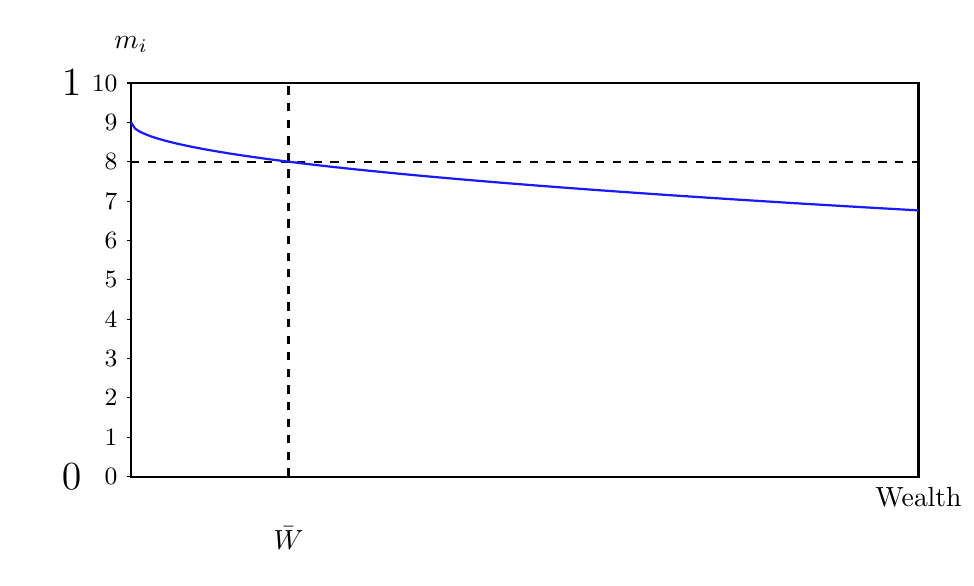
\begin{tikzpicture}[scale=.5]
%\def\bndmax{5}        %https://tex.stackexchange.com/questions/68462/filling-a-complex-region-with-tikz
%\def\bndmin{0.2}
\def\Y{10}  % height of y axis pecent
\def\W{20}  % length  of x axis
\def\Wbar{4}
\def\rbar{8}% this is the prime rate

% %Equation   \[ r_i = (A + .5 \frac{\bar{W}}{W_i})\omega\]
   % \def\Wmin{.63}  %This sets the lower limit fo the 
    \def\Wmin{(\B*\Wbar)/(\Y/\rbar-\A)} %function to keep in in bounds
	
 \tikzset{func/.style={thick,color=blue!90}}	

 \draw [thick](\W,\Y)-- (0,\Y)node[left=.5cm]{\Large$1$}node[above=.25cm]{$m_i$} -- (0,0)node[left=.5cm]{\Large$0$}--(\W,0)node[below]{Wealth}--cycle;  	% Axes box
 
 \draw [dashed, thick] (0,\rbar) -- (\W,\rbar);  	% Axes
\draw [thick,dashed] ( \Wbar,0)node[below=.5cm]{$\bar{W}$} -- (\Wbar,\Y);  	% Axes

\foreach \yi in {0,...,\Y} \draw (0,\yi)--(-.1,\yi)node[left]{\small$\yi$};
%\foreach \yi in {0,2,4,6,8,10} \draw (0,\yi)--(-.1,\yi));
%node[left]{\small$\yi$};
%\foreach \yi in {0,2,4,6,8,10}node at (-.1,yi) {{10*yi}} ;
\draw[func,domain=0:\W] plot [samples=200] (\x,(9-\x^.5/2);

 \end{tikzpicture}
\caption{Individual borrowing ratio $m_i$ as a function of wealth (in tenths)}
 \label{Fig:Borrowingratio}
\end{figure}


\subsection{Individualized borrowing rates}\label{SS:BorowingRate}
 $r_i$ 
 
 $r_i$ should depend on  both the person's income and their assets compared to others. The median after-tax income of Canadian families and unattached individuals was \$66,800 in 2020 according to Statistics Canada's \href{https://www150.statcan.gc.ca/n1/daily-quotidien/220323/dq220323a-eng.htm}{Canadian Income Survey, 2020}.  \href{https://www150.statcan.gc.ca/t1/tbl1/en/tv.action?pid=1110005501}{Data released in 2020 by Statistics Canada} indicates that the top 1\% of Canadians made, on average, around \$512,000 in a single year. \href{https://www150.statcan.gc.ca/n1/daily-quotidien/201222/dq201222b-eng.htm}{Survey of Financial Security, 2019}.

 A study by Statistics Canada found that the typical Canadian household now has a median net worth of \$329,900, while the average net worth in Canada is \$738,200. \href{https://www150.statcan.gc.ca/t1/tbl1/en/tv.action?pid=1110005501}{High income tax filers in Canada}

\subsection{Computing the income constraint on interest rates}\label{SS:YWealthConstraint}
$r_i$

In our model, we  tie the individual cost of capital,  $r_i$ for agent $i$, to a prime rate, $\bar r$ or the bank's target rate, $r^{target}$, prime plus 1\%, say. and to individual wealth. Figures~\ref{Fig:Borrowingrate1} and ref{Fig:Borrowingrate1} illustrate a couple of possible  cost-of-borrowing models roughly consistent  with the stylized facts about lenders. 

\begin{align}
 r_i =  &  \left(A + B \frac{\bar{W}}{W_i}\right) \bar r       \label{eq:incomeandr1}  \\
 r_i =  &  \left(\bar r - A + B *\frac{\bar W}{W_i - C}\right) \label{eq:incomeandr2}  \\
\end{align}
Where $\Bar{W}$ is mean wealth and $W_i$ is individual wealth. In Equation~\ref{eq:incomeandr2},  A determines y-shift, B, the scale, and C the  x-shift for the curve.


\begin{figure}
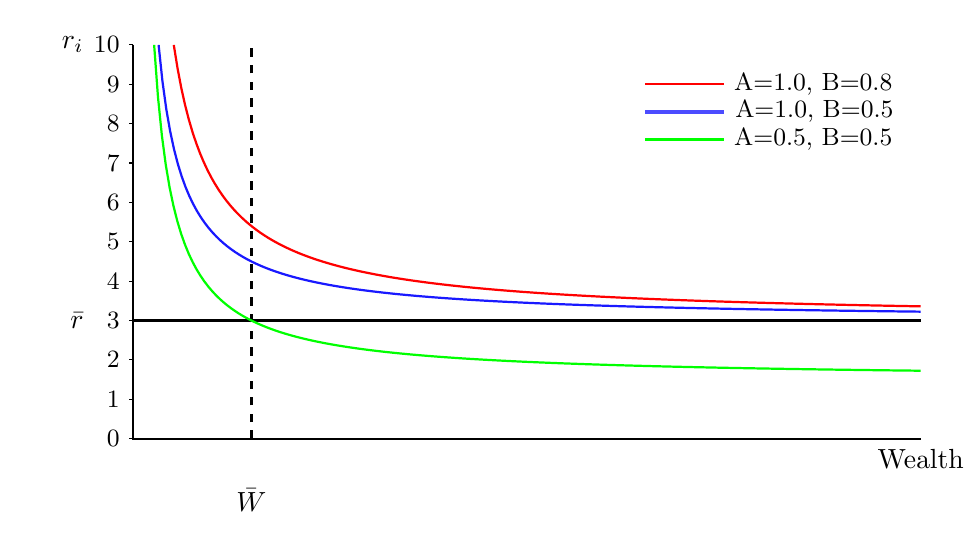
\begin{tikzpicture}[scale=.5]
%\def\bndmax{5} % https://tex.stackexchange.com/questions/68462/filling-a-complex-region-with-tikz
%\def\bndmin{0.2}
\def \Y {10}    % height of y axis as a pecent
\def \W {20}    % length  of x axis
\def \Wbar {3}  % mean wealth
\def \rbar {3}  % the prime rate 

% Equation   \[ r_i = (A + .5 \frac{\bar{W}}{W_i})\omega\]
\def \Wmin{.63}  %This sets the lower limit fo the 
\def \Wmin{(\B*\Wbar)/(\Y/\rbar-\A)} %function to keep in in bounds
\tikzset{func/.style={thick}}	

% Axes
\draw [thick] (0,\Y)node[left=.5cm]{$r_i$} -- (0,0)--(\W,0)node[below]{Wealth};  
\foreach \yi in {0,...,\Y} \draw (0,\yi)--(-.1,\yi)node[left]{\small$\yi$};
\draw [thick] (0,\rbar)node[left=.5cm]{$\bar r$} -- (\W,\rbar);  	% Axes
\draw [thick,dashed] ( \Wbar,0)node[below=.5cm]{$\bar{W}$} -- (\Wbar,\Y);  	% 

\def \A {1.0}  \def \B {0.5} %BLUE
\draw[func,domain=\Wmin:\W, color=blue!90] plot [samples=200] (\x,{(\A+\B*\Wbar/\x)*\rbar});
\draw [ultra thick, color=blue!70 ](13, 8.3)--(15,8.3)node [right, black] {\small A=\A,\ B=\B};

\def \A {0.5} 
\def \B {0.5} % GREEN
\draw[func,domain=\Wmin:\W, color=green] plot [samples=200] (\x,{(\A+\B*\Wbar/\x)*\rbar});
\draw [thick,  color=green](13, 7.6)--(15,7.6)node [right, black] {\small A=\A, B=\B};

\def \A {1.0}  \def \B {0.8} % RED
\draw[func,domain=\Wmin:\W, red] plot [samples=200] (\x,{(\A+\B*\Wbar/\x)*\rbar});
\draw [thick,  color=red](13, 9)--(15,9)node [right, black] {\small A=\A,\ B=\B};
% KEY
\end{tikzpicture}
\caption{Individual borrowing cost as a function of wealth}
\label{Fig:Borrowingrate1}
\end{figure}


\begin{figure}
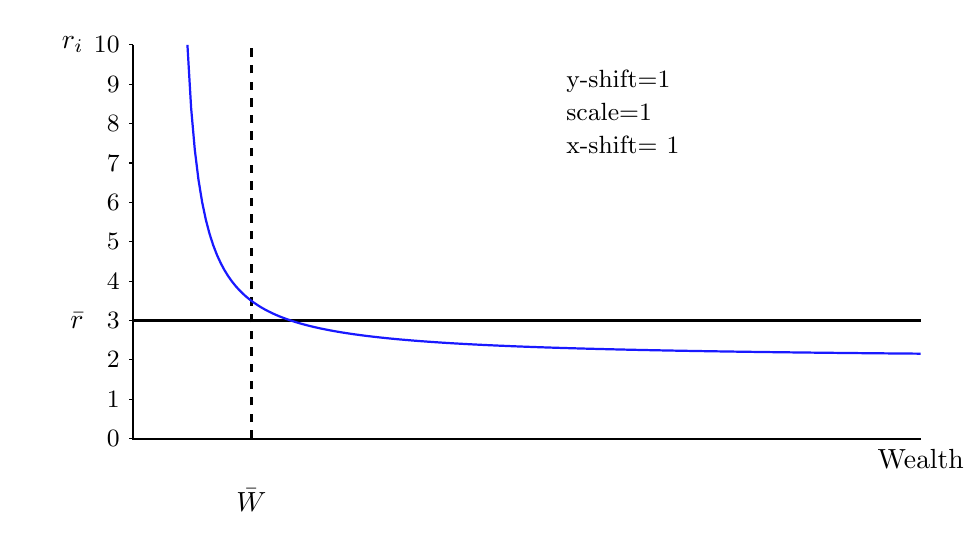
\begin{tikzpicture}[scale=.5]
%\def\bndmax{5}        %https://tex.stackexchange.com/questions/68462/filling-a-complex-region-with-tikz
%\def\bndmin{0.2}
\def \Y {10}  % height of y axis pecent
\def \W {20}  % length  of x axis
\def \Wbar {3} % meam wealth
\def \rbar {3}% this is the prime rate 

%\def \Wmin{(\B*\Wbar)/(\Y/\rbar-\A)} %function to keep in in bounds
\tikzset{func/.style={thick}}	
	% Axes
\draw [thick] (0,\Y)node[left=.5cm]{$r_i$} -- (0,0)--(\W,0)node[below]{Wealth};  
\foreach \yi in {0,...,\Y} \draw (0,\yi)--(-.1,\yi)node[left]{\small$\yi$};
\draw [thick] (0,\rbar)node[left=.5cm]{$\bar r$} -- (\W,\rbar);  	% Axes
\draw [thick,dashed] ( \Wbar,0)node[below=.5cm]{$\bar{W}$} -- (\Wbar,\Y);  	% 

\def \A {1} %vertical shift aroung \rbar, the prime rate
 \def \B {1}  % Scales the exponential curveBLUE
 \def \C {1}  %right shift  
% \def \Wmin {.4+\B}  %This sets the lower limit fo the 
\def \Wmin {(\B*\Wbar)/(\Y-\rbar+\A) +\C} %function to keep in in bounds

\draw[func,domain=\Wmin:\W, color=blue!90] plot [samples=200] (\x,{\rbar-\A+\B*\Wbar/(\x-\C))});
\node  [align=left, text width =2cm ] at (13, 8.3) {\small y-shift=\A \newline scale=\B \newline x-shift= \C};

 \end{tikzpicture}
\caption{Individual borrowing cost as a function of wealth II}
\label{Fig:Borrowingrate2}
\end{figure}

The rates $\delta,\ \sigma,$ and $r$ depend on the period, $T$. 

\section{Incorporating growth and discounting}
%We need a time period T for calculations. For use in any calculation, 

With a price-growth rate of $\dot P$ per year, the growth over $T$ years is $(1+\dot P)^T$, and  %and a 5 year mortgage period, 
the expected price at the end of the period is:

\[P^e_T=P_0(1+\dot P)^T\]

If, for example price growth is 10\%, $\dot P= 0.1$, the {capital gain}, or growth, over a 5-year mortgage term is 0.61051 $\approx$ 60\% of the original price, $P_0$.

If we want the compounded interest rate person $i$ the term T,
\[r_i^T=(1+r_i)^T\]
% This is the value we use in equation~\ref{EqBidPrice}.

If person $i$  discounts at a discount rate $r^\delta$, the present value of a receipt at time $t$ is calculated by using the \textbf{discount factor} $\delta_i^T$.

\[\delta_i^T= \left( \frac{1}{1+r_\delta} \right)^T \]
%\[\delta_i^T= \sum_{\tau=0}^{\tau=T}\left( \frac{1}{1+r_\delta} \right)^\tau \]
 
These can be combined into a function %\delta that  gives a single discounting factor  for a value  like future price that is both growing and being discounted over several (T) periods:
\[ PDV(P^e_T)=P_0\left( \frac{1+\dot P}{1+r_\delta} \right)^T \]
This PDV function specifically combines any expected rent increase, the individual's discount rate and the mortgage term into a single operation.

\subsection{Mortgage availability}
For home loans, many personal finance experts recommend total housing costs account for less than 28\% of your \textbf{gross} household income, This gives us an \textbf{income-based  mortgage maximum} of \[M^{max}_Yi = \frac{0.28*(\omega+w)}{r_i}\] It is the maximum the bank will let you pay.

We assume $r_i$ is based on the individual's assets, on relative wealth. Where is it calculated for the householder or the bank?

We get a \textbf{price-based mortgage maximum} \[M^{max}_P = 0.8P_0\] where $P_0$ is the actual sale price. This is based on the maximum amount of risk that the bank is willing to take on. ($P_0$  will not always be the same as the asking price or the warranted price.)


\section{Table}

\renewcommand{\arraystretch}{1.5}
\begin{tabular}{rlrr}\
Symbol         & Name                                 & Value      & Formula  \\ \hline
$m_i$          & Individual borrowing-ratio           & 0.75-0.85  & $M/P^{ask?}$ \\
$M^{max}_Yi$.  & Maximum mortgage based on income     &            & $\frac{0.28(\omega+w)}{r_i}$ \\
 $M^{max}_P$   & Maximum mortgage based on the price  &            & $0.8*P_0$ \\
$IS$           & Income share for housing debt        & 0.25-0.35  & Missing? \\
$\rho$         & Rent ratio                           &            & $\frac{\omega-tau*d_i}{P_0}$ \\
$\kappa $      & Operations ratio                     & 0.1-0.3    & e.g. $ 0.2\frac{\omega-tau*d_i}{P_0}$ \\
$\sigma$       & Tax ratio                            & 0.25-0.35  & e.g. $ 0.3\frac{\omega-tau*d_i}{P_0}$ \\
$\dot P $      & Price growth                         & []         & $\frac{P_t-P_{t-1}}{P_{t-1}}$\\
$P^T_e$        & Expected price in T years            &            & $P_0(1+\dot P)^T$ \\ % *** WAS $P^e_T$ 
$r_i^\delta$   & Individual discount rate             &            & To assign \\
$\bar r$       & Prime interest rate                  &            & \\
$r_i$          & Individual borrowing-rate            &            & \\
$r^{target}$   & Target interest rate                 &            & $\bar r + margin$ \\
$\delta_i$     & Discount factor for T                &            & $\left(\frac{1}{1+r_i^\delta}\right)^T$ \\
\end{tabular}
\renewcommand{\arraystretch}{1.0}


todo look for $P^e_T$ 

%==========================EXAMPLE=========================== https://www.kaggle.com/code/prateekmaj21/basic-financial-calculations-using-python/notebook
  
% def compound_interest(p,r,t):  %EXAMPLE
    
%     print('Amount: ', p)
%     print("Rate of Interest (Per Annum)", r)
%     print("Time (In Years): ",t)
    
%     a= p*((1+r/100)**t)
    
%     ci= a-p
%     print("Final Amount: ", a)
%     print("Compound Interest: ", ci)
 

\section{Transportation costs}
Transport costs have two parts:
1) fuel and vehicle costs per km
2) time costs per km

\subsection{Vehicle related costs}
Use one year as the wage period, converting transportation costs per km to annual cost for consideration in the household budget. Starting with the cost per km, calculate the cost per year:

\textbf{cost per km =$\textit{t}$}:. \$0.59   (from  Ontario data, 2021). sensitive to congestion, use of subways (\$5 /day?), 

 \textbf{work trips per year} 2 way * 5 days/week * 50 weeks work days = 500. [range: 450-550]

\textbf{cost per km-year} = work trips per year*cost per km

=\$0.59/km*500 trips/year  =  \$295/km year 



\subsection{Time costs}
\textbf{time per km}. range: 20km/hr -> 3min/km, 40km/hr -> (1.5min/km - 3min/ km)per trip 

(New York rush hour is much slower:  4-9km/hr ->6-15 min/km)

\textbf{time  per km-year} = work trips per year*time t per trip = 500* 3min  = 1500 min/km year = 25 hours= 3-3.5 days/km
 
\textbf{time cost per km-year} =  (days per km-year /work days/year)*wage premium per year  = 3/250 = 0.012 years/km year. ?

\textbf{money cost of time per km year} 

=time cost per km-year* wage(including subsistence) 

= 0.012 year* wage per year

\subsection{Total cost per km year of commuting for one agent}
\textbf{money cost of time per km year + \$295/km year * distance} \\
= (0.012 w+ \$295)/km year 
    \begin{quotation}
    \textbf{Example}
    To get a sense of the required wage if we have this annual cost structure, assume city\_extent $d^*$ is 30 km. At this point the transport cost is equal to the wage

\[(0.012 w+ \$295)/km year)*30 =  w\] 
\[.36w+ 8850=w\]
\[w=13828.12\]
        \begin{quotation}
        \textbf{PLAUSIBILITY CHECK}
This is plausible land rent, but does not include building rent. 
Capitalized at 5\% this house is worth \$ 276,562, a fairly cheap house 30 miles from city centre
        \end{quotation}
    \end{quotation}

{\color{red}
\subsection{? Value of $t$ to use in model}}
\[ \tau=(0.012 w+ \$295)/km year \]


% % \chapter{Amenity}\label{chapter-amenity}

In this chapter, we discuss how amentity might be treated in this model. 
% from Ricardo_Rent_and_Roemer_3.tex
In our base model,  an urban wage premium is the only labour attractor. Transportation costs to the urban center determine land values. Effectively in our base model, we have set the level of amenities to zero  to focus on the productivity effects. The wage premium provides a reason to find housing in the city and to travel to the city centre to work. Housing choice, however, in reality is always the purchase of a bundle of characteristics such as location, building space, yard, local density and local \glsdisp{amenity}{amenities}. Stegman  found that ``a large majority of families who have recently moved to the suburbs are more concerned with neighborhood quality than with accessibility to other parts of the metropolitan region.'' 
``There is evidence that the amenities offered by a city enhance its growth'' \cite{clarkAmenitiesDriveUrban2002, falckPhantomOperaCultural2011} and that amenity effects themselves scale superlinearly \cite{kraemerCulturalSustainabilityUS2022}.

Kaufmann et all \cite{kaufmannScalingUrbanAmenities2022} investigated the general statistical patterns in the quantity and spatial distribution of different urban amenities including public spaces and institutions as well as businesses, which all provide different services to urban populations, such as restaurants, parks, or universities.  They argue that amenities are in fact central for generating and supporting economic agglomeration effects, attracting investment to ``developing neighborhoods, promoting economic growth, supporting innovation clusters and facilitating businesses linkages.'' 
They show that the aggregate quantity of amenity infrastructure (not amenity supply)  in an urban area scales sub-linearly with population size across US metropolitan areas.\footnote{When they disaggregate, however, they find that for approximately 74\% of amenity types, they cannot reject linear scaling. Four percent exhibit super-linear scaling. They list take-away restaurants and travel agents in this range. Sub-linear scaling is associated with libraries, universities, and movie theatres.} This strongly suggests there are scale economies in amenity provision.\footnote{The model they use is the same as the one used to demonstrate that a scaling law holds for urban GDP. Instead of GDP, however, the dependent variable is a measure of amenity density based on data extracted from a unique new Google Places dataset, Google Places API (2012).} 


The amenities offered by a city can be seen as a form of non-market, non-monetary income \cite{kaufmannScalingUrbanAmenities2022}.  The non-market component of household incomes affects choices. Greater consumption amenities in a city will make workers willing to accept lower wages or higher rents. For firms,  lower wages mean lower costs. Thus,  higher amenity levels may lead to lower money wages as workers trade amenity for money income. With lower wages, more workers can be hired leading to higher output and a larger population \cite{pugaMagnitudeCausesAgglomeration2010}. 
When positive urban amenities prevail, rents and housing prices will be higher in larger cities, but wages may be unaffected \cite{robackWagesRentsAmenities1988, dalmazzoAmenitiesSkillbiasedAgglomeration2011}.
%localized productive advantages will make firms willing to accept higher wages and higher rents  


%It involves budget allocation. If we hold the housing budget constant and add an explicit urban amenity, other variables must adjust. 
% Higher wages make residents better off whereas higher rents make them worse off. Thus, 


%.  This helps disentangle the consumption amenities from the productive advantages of big cities.


In our base model,  To introduce amenities we can simply add an amenity value $A$ to the estimated value of any home. The value can depend on location, allowing for `better' and `worse' neighbourhoods,  and it can be made to depend on household attributes: a family with children might value a neighbourhood with a school or a park more highly. 

For some households, the amenity of an area may depend on the density of the city or of certain types in a neighbourhood. This is a social agglomeration effect that may work in addition to the agglomeration effect on production \cite{gurwitzCatastrophicAgglomeration2019} that we have already considered. There are also agglomeration effects in consumption goods. Larger consumer markets support more variety in goods and services. This variety allows a greater range of preferences to be satisfied. A larger city may have more production sectors and a larger array of consumer services, increasing the value received from a given income.  These closely related but different effects can be modeled by introducing an amenity term in various ways 

The amenity-induced rise in housing prices may absorb what would otherwise be consumption expenditure on other goods. Residents might accept smaller housing units for access to urban amenities.\footnote{Some costs may fall with agglomeration. There is evidence of a strong negative correlation between the total energy consumption of a city and its overall urban density \cite{newmanSustainabilityCitiesOvercoming1999}. Larson et al. \cite{larsonEnergyImplicationsCity2015} show that per-capita energy use is relatively invariant to city size when growth is driven by wages but falls modestly with growth induced by rising amenity.} In any case, there will be distributional effects as amenities play a larger role in urban agglomeration. Property owners will capture increased land rents. If amenities are funded out of taxes, the burden falls on all residents, since property taxes are very roughly related to housing consumption, but the land rents are captured by institutional owners as well as owner-occupiers and not by tenants.


%\glspl{amenity}, or non monetary income it another form of wealth,See Kaufmann et al. \cite{kaufmannScalingUrbanAmenities2022}.  and it is %, are however, an important feature of the urban system. 
% We have intentionally suppressed amenity but can add it it simply.
% (ownership effects, produtivity spilllovers, - table where you show them in the static and dynamci case with amentity)
% 2 classes of exploratin of the model in the past tho chaptered

 
%To understand amenity in our model, we need to understand it's relationship with growth, productivity, and agglomeration.
\section{Modelling amenity}

This section sketches an extension of the model to study include \gls{amenity} and suggests how it might affect results. Amenity effects can be introduced in a variety of ways. %hey might work though An economics might prefer to introduce amenity as a good in the utility function of agents.
% It might then depend on the size of the city, the size of an amenity-producing sector, the specific amenity-generating infrastructure provided by the city through taxes,  or neighbourhood effects. Each of these would take a different functional form. In our model agents are represented by their demand for housing, so the same terms would be introduced into the bid function. % In the utility framework, bids are simply derived from the utility function, so the two approaches are equivalent. %  The virtue of using the utility framework is that it begins with the question, ``What do people want?'' rather than ``What do people do?'' The first question is more productive if we want to identify different amenities that might matter.

\subsection{Through household utility}
The most direct way to incorporate agglomeration amenities is  to include what might be called a \gls{utility premium} for urban dwellers as non-monetary location income $\mathbb{A}(d; N), \die{\mathbb{A}}{N}> 0), \die[{\mathbb{A}}]{d}< 0)$ depending on distance, $d$ from the centre and urban population $N$. The second term can incorporate local amenities as well. A simple linear (indirect)\footnote{The indirect utility function is a function that depends on income and prices rather than goods and services.  Income does not generate utility, but it does generate utility indirectly' because it enables people to purchase goods and services.} utility function specified on broad income (net wage plus locational amenity) is convenient for illustration:

\begin{equation}VU(w,A)= \psi+ \omega-cd + \mathbb{A}(d; N) - T(d))
\label{eqn-u}
\end{equation}
where $w$  is an urban wage p, $T(d)$ is transportation cost from the centre to $d$.
\footnote{\cite{anasUrbanSpatialStructure1998} shows that a linear transportation cost will not  hold if congestion declines  with $d$.} 
 In most versions of the Alonzo model the `wage premium' is simply given in the urban wages and there is no amenity term. 


%\footnote{wage income, if all income goes to housing, or the share of wage income going to housing services.   (If we use a Cobb-Douglas utility function we would just replace $w$ with    $\alpha Y$, where $Y$ is household income and $\alpha$ is the share of total income. } Let  $T(d)=td$ be transportation cost with  $t>0$. 
 
\begin{figure}[t!b]
\begin{center}
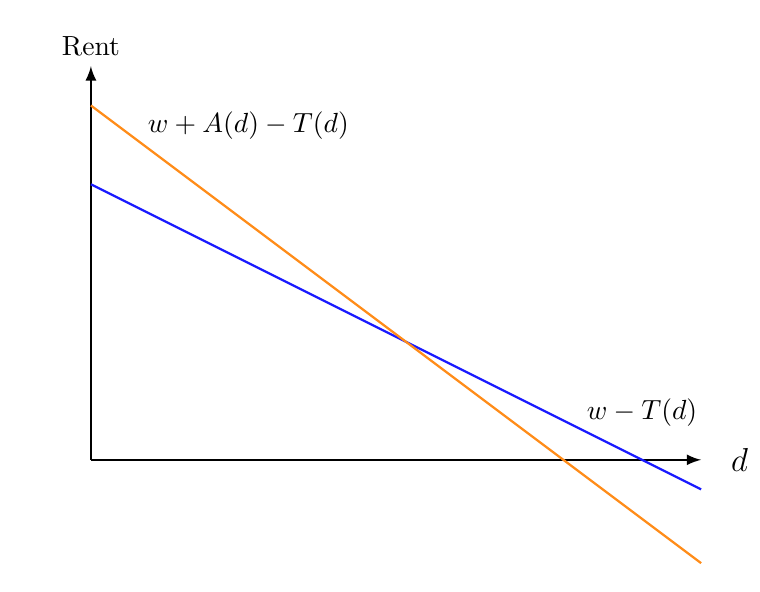
\begin{tikzpicture}[scale=.5]
\def\bndmax{5}        %https://tex.stackexchange.com/questions/68462/filling-a-complex-region-with-tikz
\def\bndmin{0.2}
\def \n {10}
\def \m {15.5}
\def \t {.5}
\def \th {1}
\def \w {7}
\tikzset{func/.style={thick,color=blue!90}}	
\draw [thick, latex-] (0,\n)node[above] {Rent}--(0,0);
\draw [thick, -latex] (0,0)--(\m,0)node[right=.25]{\large $d$};
%\foreach \xi in {0,..., \m} \draw (\xi,0)--(\xi,-.1)node[below=1]{\small$\xi$};
%\foreach \yi in {1,...,\n} \draw (0,\yi)--(-.1,\yi)node[left]{$\yi$};
%%\foreach \i in {1,4,9,16} {
	\draw[func,domain=0:\m] plot [samples=200] (\x,{\w-\t*\x});
%	\draw[func,domain=0:\m, dashed] plot [samples=200] (\x,{\w+\azero-\th*\x+\aprime*\x});

\node at (14,1.2){$w-T(d)$};
\def \azero{2}
\def \aprime {-.25}	
\tikzset{func/.style={thick,color=orange!90}}	
	\draw[func,domain=0:\m] plot [samples=200] (\x,{\w+\azero-\t*\x+\aprime*\x});
\node at (4,8.5){$w +A(d)-T(d)$};
%\node at(-.8,2) [left]{base $2^1=$};
%\node at(-.8,1) [left]{$2^0=$};
%\draw[dotted] (0,2)--(1,2)--(1,0); 
 \end{tikzpicture}
\end{center}
\caption{Rent profile with amenities}
\label{fig-amenity}
\end{figure}

 This model can produce variations on the standard result in the Alonso model. Figure~\ref{fig-amenity} illustrates a linear amenity function, $\mathbb{A}(d|N)= a-b*d$, that is convenient for illustrative purposes.  It shows how a particular amenity function might affect the rent profile, and hence city size and it allows simple experiments with the effect of increasing population on city size, wages and rents. 

In this case, amenity falls below zero in the outer regions of the city and, the geographical size of the city will be smaller. With a linear function, this happens if $\frac{a}{b} < \frac{w}{t}$. (a smaller city would have a secondary effect on wages, since with fewer workers' marginal productivity would be higher and therefore wages would rise. This would partially offset the initial decline in population.)
There would be a band of land around the city with negative amenity for commuters.\footnote{The very simple graphical result rests on several assumptions - no other housing expense, housing all the same size, wages all equal, preferences identical, transportation costs.}

The far more likely case is that $A(d) > 0$ when $w-T(d)$ falls to zero. In this case there is a band of residents around the city, outside of the population commuting to work. They do not travel to work,  do not collect a wage, but still enjoy the amenity of being close to a city. This might be a population of retired persons enjoying occasional visits and healthcare facilities.


\subsection{Neighbourhood amenity}
In Figure~{fig-amenity} the source of the amenity is at the centre of the city. We can easily imagine an amenity profile that is high for some neigbourhoods and lower for others, as in  In Figure~\ref{fig-amenity2}. The jagged area below the orange line is rent accruing to landowners. The variable rent comes not from a desire to be close to the source of the wage income but from household demand for local amenity.  
\begin{figure}[tb]
\begin{center}
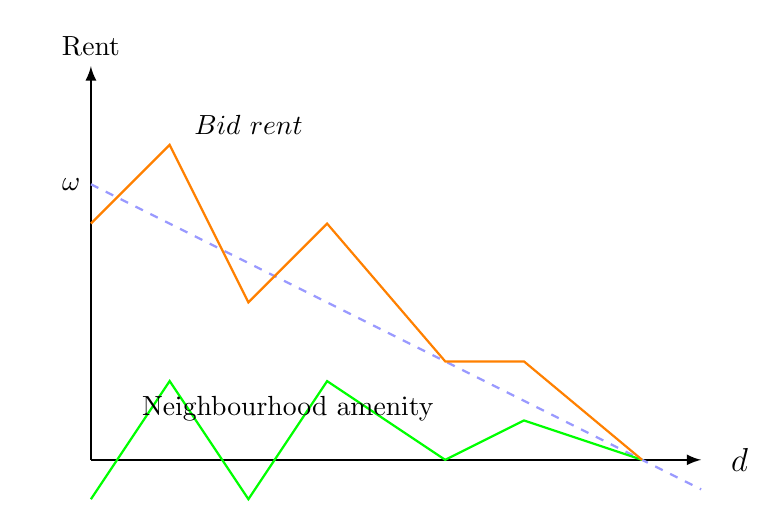
\begin{tikzpicture}[scale=.5]
\def\bndmax{5}        %https://tex.stackexchange.com/questions/68462/filling-a-complex-region-with-tikz
\def\bndmin{0.2}
\def \n {10}
\def \m {15.5}
\def \t {.5}
\def \th {1}
\def \w {7}
\tikzset{func/.style={thick,dashed, color=blue!40}}	
\draw [thick, latex-] (0,\n)node[above] {Rent}--(0,0);
\draw [thick, -latex] (0,0)--(\m,0)node[right=.25]{\large $d$};
% Basic Bid rent,
\node at(-.5,\w) {$\omega$};
\draw[func,domain=0:\m] plot [samples=200] (\x,{\w-\t*\x});
%NEIGBOURHOOD AMENITY
\draw [thick, green] (0,-1)--(2,2)--(4,-1)--(6,2)--(9,0)--(11,1)--(14,0);
\draw [thick, orange] (0,6)--(2,{7-2*.5+2})--(4,7-4*.5 -1)--(6,7-6*.5+2)--(9,7-9*.5)--(11,7-11*.5+1)--(14,7-14*.5);
\node [] at (5,1.3){Neighbourhood amenity};
\def \azero{2}
\def \aprime {-.25}	
% \tikzset{func/.style={thick,color=orange!90}}	
% 	\draw[func,domain=0:\m] plot [samples=200] (\x,{\w+\azero-\t*\x+\aprime*\x});
\node at (4,8.5){$Bid\ rent$};
%\node at(-.8,2) [left]{base $2^1=$};
%\node at(-.8,1) [left]{$2^0=$};
%\draw[dotted] (0,2)--(1,2)--(1,0); 
 \end{tikzpicture}
\end{center}
\caption{Rent profile with neighbourhood amenities}
\label{fig-amenity2}
\end{figure}
Financialization might or might not affect neighbourhood amenity. If it does it might have its effect by changing the ownership mix.

\subsection{Public provision of amenities}

Previous sections suggest amenities may work as a wage subsidy, potentially increasing output. Since employers will not willingly pay for urban amenities, some amenities may be financed publicly. It is common to introduce the cost of generating amenities as a tax on residents.  Since public amenities may be \glspl{public good} in the economic sense, the municipal government may be able to achieve significant wage economies with a small public expenditure.

A simple way to incorporate publicly provided amenities to make an amenity function that proportional to a fraction of public revenue, which is a fraction $\tau$ of the land value when municipalities depend on property taxes. Assuming a uniform property tax rate, total property tax revenue in a circular city are approximately $\tau(\phi+2/3 \omega)\pi \frac{\omega}{c}^2$. We can therefore include in the buyer's maximum bid function a fraction if this value. Property investors would not include this amenity component, but it would affect their decisions because amenity raises their net rent.

Notice that because amenity raises property values, in Ontario it does not raise tax revenue because the property tax rate is adjusted to balance the budget. This creates perverse incentives for municipalities \cite{blaisPerverseCitiesHidden2011}.


\subsection{An amenity sector}
Producing amenities takes resources. Some fraction of the workforce must be engaged in producing the amenity services. A simple approach would be to assume that the base employment that we consider demands a layer of amenities that represent the additional fraction of the population needed to provide the amenities - say 10\%  

Larger cities can support larger and more varied amenities, so that effect of amenities on property values might be larger in larger cities. At the same time, there are apparently economies of scale in the production of amenities \cite{kaufmannScalingUrbanAmenities2022}. We have no strong prior about how in amenity sector would be affected by finacialization of housing.  An effect might work through changing ownership.


\section{Research on amenities}
% There is a great deal of research on amenities. In this subsection mention a few that seemed noteworthy. 
Most of the literature on amenities deals with livability and the benefits for the individual. There is a strand in the literature, however, that links amenities to growth. In 1954, for example, Edward Ullman \cite{ullmanAmenitiesFactorRegional1954} published  ``Amenities as a Factor in Regional Growth,'' an article that came to be seen in the geographical literature over the following 50 years as prescient \cite{walcottCommentsEdwardUllman2010} for introducing the notion that amenities could be an important mobility magnet. 

Many have since extended this approach. Richard Florida, in a series of articles and books beginning in 2002 \cite{floridaCreativeClassEconomic2014, floridaEconomicGeographyTalent2002, floridaCompetingAgeTalent2005} examined the notion that urban growth depended on attracting the creative class and that in turn rested in part on the amenities a city offered. A 2008  Statistics Canada study, `Cities and Growth: The Left Brain of North American Cities,' Beckstead et al \ found substantial differences in average growth for cities with higher cultural employment and urban amenities.  Clark et al \cite{clarkAmenitiesDriveUrban2002} argue that much of Chicago's recent growth to 2003  should be attributed to reforms instituted by Mayor Richard M.  Daley explicitly linked to amenities and quality of life issues, including parks and schools. Abouy \cite{albouyWhatAreCities2016} finds that wage and housing cost differences across metropolitan areas are accounted for more by productivity than quality-of-life differences, however. 

Beckstead et al  \cite{becksteadCitiesGrowthLeft2008} identify amenities with the unexplained variastion in median urban house price after controlling for median household income.\footnote{  The basic premise would be that after conditioning on household income, variation in home prices across cities would be a function of the relative attractiveness of these places. The residuals yield a continuous ranking of cities based on the estimated variation in urban amenities.} Rappaport \cite{rappaportConsumptionAmenitiesCity2008} presents empirical evidence that amenities do support high-density levels, and that amenities cause approximately one-fifth of the cross-sectional variation in metro population density. 


% Molotch's (1976) metaphor suggests that the city is a machine geared to creating growth, with growth loosely defined as the intensification of land use and thus higher rent collections associated professional fees and locally based profits. Many urban economists, planners, and political scientists have made similar arguments (e.g., Bradbury, Downs, & Small, 1982; Mollenkopf, 1983; Stone, 1989). However, a quarter century later in the contemporary competition among US cities, the growth machine model has lost much of its power.
  


\newpage


% \chapter{Notation}
% \section{Notation for Urban and Production Sectors}
\newpage
\begin{longtable}{lp{10cm}}
\caption{Notation}                       \\
\hline           &  \textbf{Productivity} \\ \hline
$K$              &  Capital               \\ 
% $L$            &  Labour                \\
$N$              &  Population, equals labour \\ %, $L$          
%$\Lambda$    &  Labour-augmenting agglomeration effect \\
$Y=A K^{\alpha }N^{\beta }$  &  a Cobb-Douglas Production function \\ %Urban output            \\
$\alpha$         &  Elasticity of output with respect to capital          \\
$\beta$          &  Elasticity of output with respect to labour           \\ % vs effective labour
$\gamma$         &  Elasticity of agglomeration with respect to labour    \\ % , $\Lambda(n)$, for illustration \\

% $L$              &  Labour supply \\ %the number of workers, which, in the standard circular city model, equals the number of lots of size $s$  when workers live on identical individual lots. % Unless $d^{max}>d^*$ v  \frac{\pi}{s}(\frac{w}{{c}})^2 =
$n$  &  Number of workers at a firm \\
% $n_i$  &  Number of workers employed by firm $i$ \\
%$n=\sum_i n_i$  &  Number of workers, the urban population in the model \\
% $\#f=\frac{n}{n_i}$&number of identical firms \\ %not used
% $f$  &  Number of firms =1 \\
% $n =f n_i$  &  Aggregate labour \\
% $n^\gamma$ & The labour-augmenting agglomeration effect,  modelled as an exponential function of the number of people \\
% $\Lambda(n)n_i$ &  Effective labour for firm $i$ \\
% $\Lambda'=\die{\Lambda(n)}{n} $ & Derivative of the labour-augmenting agglomeration effect\\

%%$Y_i=K_i^{\alpha }(\Lambda(n)n_i)^{\beta }$  &  Urban firm $i$'s output \\

%%$Y=\frac{n}{n_i}K_i^{\alpha }(\Lambda(\sum_i n_i)n_i)^{\beta }$  &  Aggregate output of all firms in the city \\
% $\die{Y}{n}=\beta\frac{1}{n} Y  \left( 1+ \frac{n\Lambda'}{\Lambda} \right)$  &  Social marginal product of labour \\
% $Y_i=K_i^{\alpha }(\Lambda(n)n_i)^{\beta }$    &  Urban firm $i$'s output \\
% $\die{Y_i}{K_i}	=\alpha \frac{1}{K_i} Y_i $  & Marginal product of capital for firm $i$ \\
% $\die{Y_i}{n_i}	=  \beta\frac{1}{n_i} Y_i $  &  Marginal product of labour for firm $i$ \\
%%$\eta=\frac{n_i\Lambda'}{\Lambda}$  &   Marginal agglomeration effect on a firm's output of increasing it's own labour stock \\
% \hline
	% &\textbf{Amenity}\\ \hline
% $A(d, n)$   &  Agglomeration amenity          \\

\hline  0 &  \textbf{Labour market}                \\ \hline %and urban stucture??
$\psi$            &  Rural subsistence wage                             \\  
$\omega$          &  Urban wage premium          \\
${c}$             &  Transportation cost per unit distance \\ % Was $\tau$, and $trans$. Considered $\gamma, \xi, \zeta$.
$d$               &  Distance from city centre   \\
$d^* = w/{c}$     &  City extent \\ %, the maximum distance commuters will travel \\ % Maximum distance commuters will travel \\ % to get the wage premium \\
% $\mathcal{R} = \omega - {dc}$ &  Rent at distance ${d}$ \\ 
% $\zeta$          &  Population density at distance $d$     \\
% $s$              &  Lot size      \\
% $\psi$  &  ?Per-period cost of a unit of productive capital \\
% $\omega + \psi$  &  Urban wage including rural wage \\ %***
% $\textit{t}$ & {\color{red}transportation cost per km} \\%use   c?
% $w^n=\omega-{dc}$ & Wage  premium net of transportation costs \\
%% $\Omega=\frac{\omega+\psi}{\psi}$  &  Ratio of the urban wage to the  cost of capital \\
%% $\Pi$	   &  Profit \\
%% $ER$	   &  Excess return to capital \\ 
% \hline &\textbf{Spatial structure in the circular city} \\ \hline		
%% $d^{max} = \omega /{c}$  &  Maximum distance commuters at which residents enjoy the urban amenity \\
%% $d^{**} = max(d^*, d^{max})$  &  radius of the city \\
%% $U$                     &  Worker utility **\\ %, a function of location and prices \\
%% $U^{urban}=U^{rural} $  &  Migration equilibrium assumption ** \\
% \hline & \textbf{Labour market} \\ 

\hline           & \textbf{Financial market}             \\ \hline
$P_W$            &  Warranted price for a property       \\
$P_B$            &  Bid price                            \\ % was P^{bid}
$P_A$            &  Asking price                         \\
$P_M$            &  Realized market price                \\
$P_M^e$          &  Expected market price                \\
% $P$            &  Price of a property                  \\ 
% $\dot P$       &  Rate of price growth              \\ % was $\dot p$  
% $\mathcal{C}$    &  Capital gains                     \\ % was C
% $\mathcal{C}_N$  &  Net capital gain, $C -$ net rent  \\
% $M$              &  Mortgage                          \\ 
% $m$              &  Mortgage share, the share of the property price that can be borrowed, which is a function of wealth  \\ 
$\mathcal{R}$    &  Rent                              \\
$\mathcal{R}_N$  &  Net rent                          \\
${R}^w_N$        &  Warranted rent                    \\
$\rho$           &  Rent ratio                        \\
$\phi$           &  \Gls{rent share}                  \\
$\mathcal{O}$    &  Operational costs                 \\
% $\theta$         &  Operations ratio                  \\ % was $\kappa$ became b
$\mathcal{T}$    &  Taxes                             \\ % was $\Sigma, \Xi$  
$\tau$           &  Property tax share                \\ % was t then $\sigma, \xi$  b
% $\tau$            &  Annual tax rate on rent and home \\ % Was $c$ 
$r$              &  Interest rate                     \\
$\delta$         &  Individual's subjective \gls{discount factor} \\
% $W$            &  Wealth                            \\
% $\psi$         &  Fraction with rent/operating costs\\
$t$              &  Time                              \\

W & Wealth \\
m & Mortgage share \\
M & Mortgage \\
S & Savings \\
% \mathbb{C} carrying 0.28, max_mortgage share, wealth_sensitivity

$\mathbb{T}$     &  Time period                       \\

$a$       &  Share of subsistence wage  used for land and building \\
$b$       &  Maintenance share of share of subsistence wage \\ % A cost. Includes water, electricity, heat? 
% $wage_share$     & OLD Share of the agglomeration effect that goes to workers. \\

\hline
\color{black}
\end{longtable}  

\newpage

\begin{longtable}{lp{10cm}}
\caption{Rent}                                                            \\
\hline
$\omega-{dc}$                &  Warranted (economic) rent                \\
$\mathcal{R}=\omega-{dc}$    &  Equilibrium rent payment of tenant       \\
PDV                           &  Present discounted value                 \\  
$\mathcal{R}^T$               &  PDV of rent collected over period $T$    \\ 
$\mathcal{R}^T_N=(1-\kappa-\sigma)\mathcal{R}^T$  &  PDV of net rent collected over period $T$ \\
\hline
\end{longtable}

\begin{longtable}{lp{10cm}}
\caption{Bidding mechanism notation}                                          \\
\hline
$\mathcal{R}_N$  &  Net rent                                                  \\ % was NR
% $P_0$            &  Purchase price for a property                             \\
% $P^T_e$          &  Expected price at the end of period $T$                   \\
$r^{prime}$         &  Prime interest rate                                       \\
$r^{target}$     &  Investor or banks target interest rate, $\bar r + margin$ \\

$r_i$            &  Agent $i$'s personal borrowing rate                       \\
$r_i^T$          &  Agent $i$ interest rate compounded over a period $T$      \\
$r_i^{disc}$     &  Agent $i$'s subjective discount rate (which may equal $r_i$) \\
$r_\delta$       &  Discount rate                                             \\ % was $discr_i$
$\delta_i^T$     &  Discount factor for agent $i$ over period $T$             \\
$m^W$            &  Wealth-based share of home price a worker can mortgage    \\ % $= m_i(W_i)$
$m^\omega$       &  Income-based share of home price a worker can mortgage    \\ % IS_i   IS_i(\omega+\psi)$$
$m_i = min(m^W_i, m^\omega_i)$  & Mortgage, the share of home price worker $i$ can mortgage \\

\hline
\color{black}
\end{longtable}  
Notation: 
Agent counts and indices are subscripts.
Values related to time are superscripts, time as a continuous 
variable is small, a period is capitalized e.g. the period $T$ of some number of years. 
In general values are capitals, rates are small letters.

% It might be better to use the subscript $m$ for `market'.  for warranted rents



 


% Everything
\chapter[Future Work]{Future Work}
\label{appendix-future-work}



In  this chapter, we discuss potential extensions of our basic model.  Models are by nature combinatoric: every added element involves making a choice among alternative assumptions and implementations. A model incorporating in binary choices is one of an implicit family of $2^n$ alternative models. We have sharply restricted our model  in order to focus on one process of significance, financialization.  This is in part so that we can explain and justify each assumption that we use, and in part because only sharply restricted models produce understandable results. 
% Those results are condition on the specific set of assumptions to ensure that 
We have designed the model to  accommodate a range of extensions that are either theoretically or interesting or important for policy-makers. 



Figure~\ref{fig-logic-extensions} illustrates  five general types of extension. The first is to move from a static population to a model with population pressure. This appears on the left as a group of three new subroutines with connections to the elements of the model most directly affected. Some links are left out to keep the figure readable. Examples of omitted links  are the channels through which  population affects labour supply and savings.  


A second class of extension would introduce a housing production sector. This appears on the right side of of the figure linked to the banking sector. It requires adding a dynamic housing  stock. 

A third major class of extensions, separable from production is to introduce variation of housing form,  density and amenity. Zoning restrictions and building codes are related. Many questions about who gets what housing arise at this point. 

{\newpage\thispagestyle{empty}
\vspace{-1.5cm}
\begin{figure}
\vspace{-4.5cm}
\begin{adjustwidth}{-0.24\textwidth}{-0.2\textwidth}
\centering
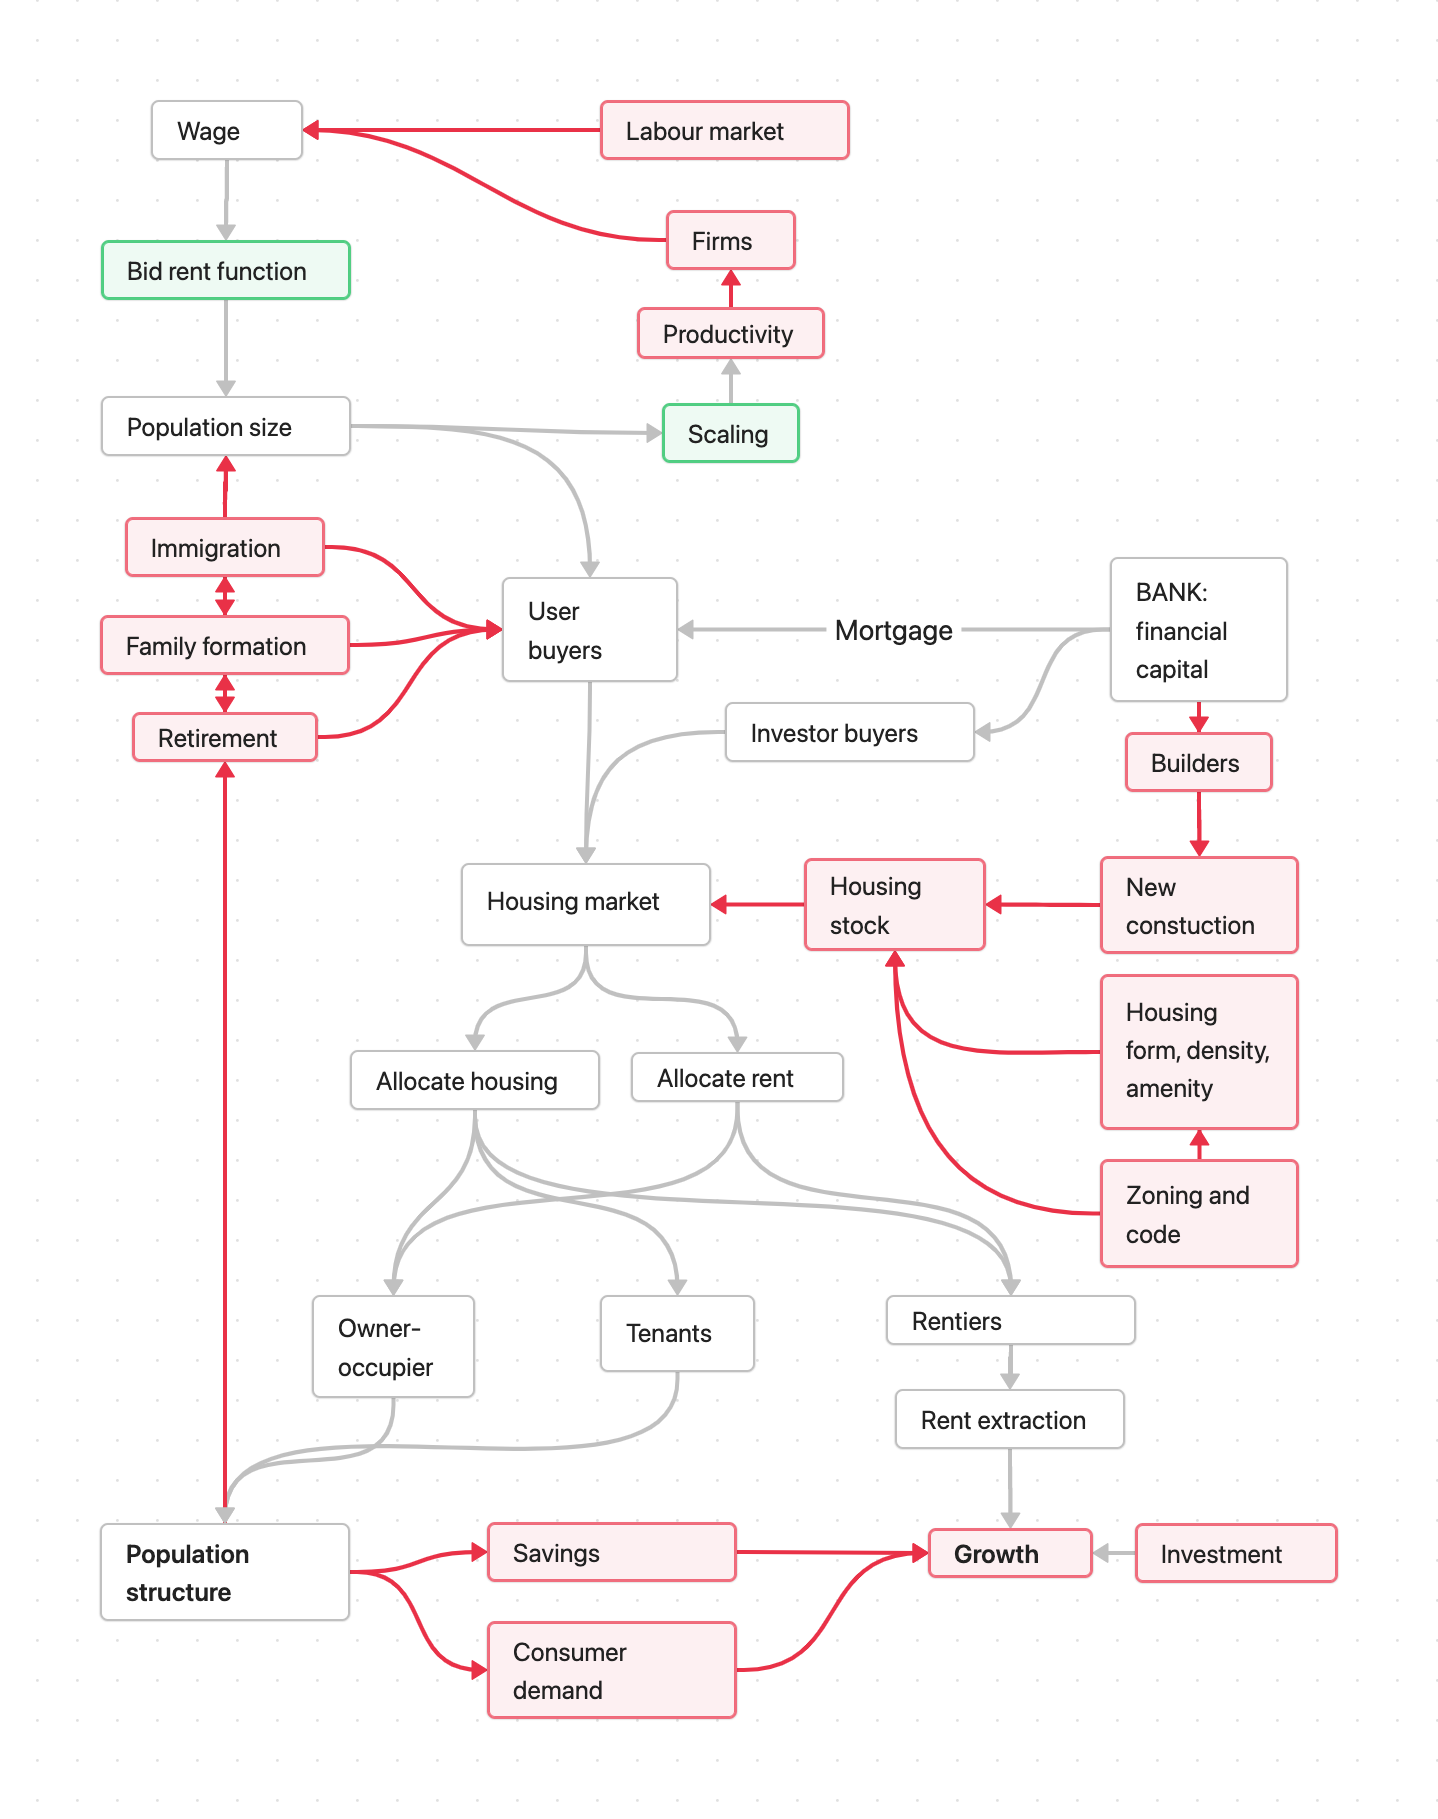
\includegraphics[scale=.22]{fig/extensions.png}
\end{adjustwidth}
\caption{Extensions}
\label{fig-logic-extensions}
%\pagestyle{headings}
% \usetikzlibrary{positioning}
%\begin{tikzpicture}[remember picture,overlay,shift={(current page.north east)}] \node[anchor=north east,xshift=-1cm,yshift=-1cm]{\includegraphics[width=1cm]{example-image-a}};\end{tikzpicture}

\end{figure}
}


At the bottom of the figure we introduce consumer demand linked to the population structure and feeding back to growth. Savings behaviour becomes more  complex when consumer demand is made endogenous and with as more complex population structure.

The fifth block of extensions illustrated in Figure~\ref{fig-logic-extensions} would replace the simple, scaling-based transmission mechanism in the Alonzo-Jacobs cycle with explicit firm and labour market behaviour. This class of extensions is obviously linked to population structure. It leads to consideration of firms that produce different products, some for export some for the local market, and to multiple types of labour.

Linked to the labour market and production system is the possibility of introducing competing cities. 

It should be clear that each of the extensions we suggest is potentially as complex as our core model, and each brings with it a collection of additional assumptions. We would argue that none of them would change our qualitative results greatly, although each would deepen our understanding of mechanisms and of the detailed impacts.


\section{Population pressure } 
Our basic model does not have a growing population. This conveniently allows us to isolate certain effects of financialization. Population pressure is one of the drivers of financialization because it amplifies speculative gains, however. As a result, one of the first extensions must be  to introduce population pressure.

There are two sources to consider: 
\begin{enumerate}
\item agglomeration effects that increase the wage and attract workers faster than the housing stock can respond. 

Worker agents from outside the city can always consider moving and accepting a job. 
% QUESTION - how to manage the flow of new agents?
%, or can make more from rents and moving away
\item immigration pressure
\end{enumerate}
under the  first, agglomeration economies drive population while under the second, population growth may drive agglomeration.

The growth of the housing stock will generally lag population growth, generating price effects and stock dynamics.

Agents will respond to increases in demand conditions. The perception that the market is tight or that prices are rising may lead to higher bids and reservation prices and shift results in favour of sellers.  


%Buyers could consider neighbourhood pressures, demographic changes, changes in job location, desire for amenity etc. in their assessment of housing need. 

%With multiple bids agents can place the most competitive bids on those homes they prefer. If they have higher urgency they place strong bids on more homes. 

%Next buyers request a selection of homes to consider from a real estate agent. Those with higher need for housing look at more homes. The real estate agent offers a selection of homes based on the agent's requirements. A randomness parameter determines how many divergent houses are also considered. When the parameter is 1, the selection of homes is fully randomized, When it is 0, the agent sorts all available homes and offers those which fit the agents budget, space, and other requirements best.


\subsection{Retirement investors and private investment properties}
The simple population turnover in our model can be replaced with a more complex set of possibilities at the agent level.  At retirement,  agents can be allowed to may choose between selling their home, renting it as an income property, or if there is sufficient amenity value for them, staying in the city. Implementing these choices complicates the agent decision and the resulting housing distribution but require few changes to the rest of the model.

\section{Housing production}

\section{Differences in density, housing form, and neighbourhood amenity}
Much of what is interesting in a city is the rich variety of housing forms and neighbourhoods and the varied populations that occupy them. Our model has a single form of housing and an undifferentiated populations, allowing us to differentiate the housing system in specific ways and study the interactions between the built world and the population. We are convinced that few of the possible extensions could affect our qualitative results. 

Nonetheless, in our agent based model, in which every lot is  addressable, it is simple to introduce zoning boundaries, local amenities, different densities or housing qualities and homes of different sizes. Hundreds of experiments are possible exploiting  the extensibility we have carefully conserved.  

We can ask what would be the effect of a hard zoning boundary and what would be the effect of suddenly relaxing it. We could explore the effect of speeding the rate of conversions from one size  home to another, or of locating high density pocket on a transportation route. Many significant urban policy questions could be examined with a limited amount of additional programming. 

\section{The consumer city}
Much of the demand for what is produced in the city is local consumer demand.  Our model has assumed there is production only for a perfectly elastic export demand. Consumer needs are buried in the subsistence wage. 

A minimal extension would be to introduce a second sector representing local consumption demand. A share of locally generated income would support production for the city's population. The labour force would be split between the two sectors and both productivity and wages might differ across sectors. 

A more complex treatment would introduce a range of service, entertainment and retail producers. This might be done monopolistically competitive firms \'a la Dixit and Stiglitz \cite{AvinashK.Dixit1977MCaO}.



\subsection{Distribution of rents}
Rents go to landowners, with a share taken for maintenance and taxes.
Rents may also be taxed, could be shared between multiple owners, etc.
 %\note{REPHRASE? rent is  extracted from the coalition of capital and workers.} % Rents may also be taxed, could be shared between multiple owners, etc. 
%The rents are captured by landowners.  The capture of rents by landowners is common buy not necessary. 
In principle the gains from urban productivity and amenity can be allocated as social wealth through shared ownership, as is often done on a small scale with cooperatives and land trusts, distributed to all citizens through something like a social wealth fund, or captured in taxes or fees as Henry George suggested. 
%The rents would otherwise go to labour and capital.





\subsection{Urban Savings - Contributions?}
THIS IS A CONTRIBUTION, BUT ALSO A DISCUSSION OF ONE WAY THIS WORK COULD BE EXTENDED, MIXED WITH A BIT OF MODEL DESCRIPTION

Conventional growth models specify a savings/investment mechanism at the national level. To our knowledge, this has not been done for the city level. We require  savings at two levels. First, since we want to incorporate  households home ownership and a relationship to the financial sector through mortgages, We specify a savings rate out of the spending we have isolated in the `subsistence wage' This means that both urban and rural workers accumulate savings, that savings are age-dependent, making the size of mortgage available also age dependent. 

Homeowners in addition have equity $E=P-M$ in their homes.  ({\color{red}Should newcomers also have equity? or is it built into the savings. Clarify this.} 

A second level of saving is the  investment in capital out of the city surplus. Even raising this question puts us into terra incognita. There are many  channels through which surplus flows into productive investment in the urban contest. One is through public investment in infrastructure. We have discussed how falling transportation costs increase surplus generation. Investments like this are made slowly and take effect over time periods much longer than our model is concerned with.  We can set a property tax rate   that we will assume is sufficient to maintain the stock of infrastructure.

Public and private investment in human capital is largely urban as well, but as with infrastructure, investment and response take effect over time periods much longer than our model is concerned with. 

Private sector innovation in technology, marketing, or products draws on local saving less but still significantly on local savings. We have little in the way of theory or empirical research on this channel. Lags between investment and any rise in the urban wage premium are almost certainly long and variable. 

We deal with this issue by linking local capital ownership with the scale factor. It is known that local ownership is associated with local investment. We will assume that local capital ownership, which consists in part of local ownership of the housing stock, can be proxied by homeowner equity as a share of local. 

\subsubsection{savings and retirement behaviour}
Agents fund their retirement from savings, as well as returns on their home if they have one to sell. Savings may be invested in a pension fund, or in local property,  depending on expected risks and returns. In the real world, financial institution manages most pensions, investing in the market or in property.  All this institutional structure is probably most easily handled by implementing a savings account for each agent. We are not interested in the detailed investment behavour for the financial sector.% either in the stock market, or in pensions.

%Institutional and individual investors can access debt. %

We could also consider a case where outside money can come under institutional management, not just local retirement savings. A parameter would control the inflow of additional money beyond local investment in the pension fund. 



\section{Making  labour market and firm behaviour explicit }
We have carefully developed the link between neoclassical growth theory and the literature on urban scaling \cite{bettencourtIntroductionUrbanScience2021} and  We then imposed the scaling result on our model.  We force the model to conform to the empirical data on the relationship between population and productivity. This amounts to black-boxing the entire production and labour demand sector as well as the construction and housing production sector. 

This made sense because our focus  was on the housing market and the financial sector, but the model we have constructed will allow us to ``fill the black box'' with more complete models of the production and labour market to see how they compare to the empirical data. 

The  scaling  literature also provides relationships between density and population and infrastructure cost and population that we can explore in the same way.

In the scaling literature, these relationships are increasingly theorized in terms of network effects, which is perfectly consistent with the Jacobs analysis and the more recent neoclassical growth modeling.


\subsection{The transmission puzzle}

The transmission of productivity increases arising from agglomeration effects  to the urban wage through firms, can be modelled in many ways. The agglomeration effects are external to the firm and therefore likely to be unexpected. If  firms underestimate the marginal product of labour, labour productivity will be greater than expected, output will be higher than planned output, and revenue and profits will therefore be higher than expected. Excess demand will attract more productive capital which in turn will demand more labour,  Rising labour demand drives up the wage. The agglomeration effect driving growth is essentially a public good in which individual firms will under-invest. This raises a policy challenge that we leave for others. CLARIFY - ALSO STILL A FOOTNOTE IN MODEL SECTION. CUT OR REF THEiR IF MOVING HERE.

 It is straightforward to compute the rate of excess return for  this model. 


\begin{figure}
    \centering
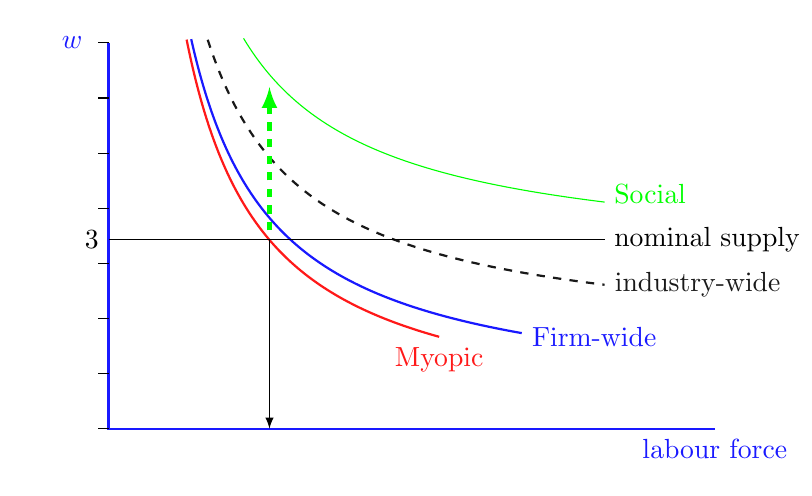
\begin{tikzpicture}[scale=.7]
%\def\bndmax{5}        %https://tex.stackexchange.com/questions/68462/filling-a-complex-region-with-tikz
%\def\bndmin{0.2}
\def \Y {7}  % height of y axis pecent
\def \W {15}  % length  of x axis
\def \Wbar {3} % jmeam wealth
\def \omega {3}
\def \A {1}  %was .5
\def \B {.5}

\draw [thick, color=blue!90] (0,\Y)node[left=.2cm]{$w$} -- (0,0)--(\W-4,0)node[below]{labour force};  
 \foreach \yi in {0,...,\Y} \draw (0,\yi)--(-.2,\yi)node[left]{};
 
\tikzset{func/.style={thick,  color=blue!90}}
% \draw[ func, domain=.2:\W-6] plot [samples=200] (\x, 2*\x^.5)node[below=.1, right]{SUPPLY};

\tikzset{func/.style={  color=green}}	
\draw[func, domain=2.45:\W-6] plot [samples=200] (\x, 10/\x+3)node[above=.1, right]{Social};

\tikzset{func/.style={thick, dashed, color=black!90}}	
\draw[func,domain=1.8:\W-6] plot [samples=200] (\x, 10/\x+1.5)node[ right]{industry-wide };

\tikzset{func/.style={thick, color=blue!90}}	
\draw[func,domain=1.5:\W-7.5] plot [samples=200] (\x, 10/\x+.4)node[below=.05, right]{Firm-wide};

\tikzset{func/.style={thick,color=red!90}}	
\draw[func,domain=8.5/6:\W-9] plot [samples=200] (\x, 10/\x)node[below]{Myopic};

\draw[](0,3.425)node[left]{$\omega$}--(9,3.425)node[right]{nominal supply };
\draw[thin,latex-](2.92,0)--(2.92,3.425); %a vertical labour supply
\draw[ultra thick,dashed, green,-latex](2.92,3.6)--(2.92,6.2);
%\draw [blue,  thick](13, 8.3)--(15,8.3)node [right, black] {\small A=\ 1,\ B=0.5};
%\draw [green, thick](13, 7.6)--(15,7.6)node [right, black] {\small A=.8, B=0.8};

%\node at (5,-1.5){Resulting in  profits, expansion, and/or entry: the city grows};
 \end{tikzpicture}
\caption{Multiple marginal products.}
\label{fig-marginal-products}
\end{figure}



Figure~\ref{fig-marginal-products} illustrates the problem. We can  make a distinction between the myopic marginal productivity curve observed by at the shop floor level and  the firm-wide effect of adding a worker. The red curve labeled ``Myopic'' represents the declining direct marginal productivity of labour as in might be observed by a shop manager, who could report how much more output one with one worker one lathe would produce. The blue line above it labeled ``Firm-wide'' represents the actual effect on firm productivity that arises because the new worker makes other workers in the firm more productive. This addition to output would be observable for managers reviewing the firm's performance over time. ' 

We can go on to consider the slower and distributed effect on closely related firms, which would raise any estimate of marginal product.  If there are 10 other firms and a new worker  has a small spillover effect  $\epsilon$ on each,  the spillovers raise the industry  marginal product  by $10\epsilon$. Each of the  10 other firms  enjoys  an additional $10\epsilon$ gain in the marginal product of their workers. This should lead to additional hiring by other firms.

Finally, expanding our view another step, we notice that if each of the  10 other firms hires one worker who produces an additional  $10\epsilon$ gain in output for all firms, the total spillover effect would rise by $100\epsilon$. The social marginal product of a single hire is indicated by the green line. 



\section{The system of cities}
Modern cities are not lonely and autarkic  beasts wandering their own exclusive territory and unconnected to others of the species. They are one is a global system of cities that compete and complement each other. Information, capital and even labour flows between cities are large. Henderson Abdel-Rahman\cite{Henderson1972Sizes}, Abdel-Rahman \cite{abdel-rahmanAgglomerationEconomiesTypes1990}, Fujita \cite{fujitaMonopolisticCompetitionModel1988}, Fujita, Krugman, and Venables \cite{fujitaSpatialEconomyCities1999}, and Fujita and Thiess \cite{fujitaEconomicsAgglomeration1996} among others provide models for expandingh the model in this direction.



\subsection{Taxes, municipal government, public goods, and productivity,}
This is a major issue with considerable development in the economics literature. Property taxes reduce the net locational value that flows to an individual owner but provides services and wages that make the city attractive. 

(create a regime where particular groups have an advantage)

Localized tax advantages can move a share of financialised investment into private consolidation of land.
including the structure of taxes for investment properties, institutional investors, individuals, etc.




\section{TO  METHODOLOGY?: Distribution}% not the right word
ABMs can be run multiple times to produce distributions of expected outcomes, which makes them valuable in planning exercises. They also do not require that we use a representative agent to make them tractable. Our model is intended to be elaborated  for such use. 

extensions
what it is
why it would be great to model
why it doesn't matter for our core results

\section{A possible typology of models and experiments}
While there  are many variations on the basic urban model and many potential experiments with each model there are only a few of immediate interest if the goal is to text the ``resilience'' of equilibria.

These models may exhibit irreversibilities in variables such as distribution, homelessness, city form, and class structure. 

The basic strategy for examining the system resilience is to shock a model (experiment) and then see if diagnostic variables recover. (This needs more precise expression.)

The first task is to select a subset of models an experiments that are of particular interests with respect to.

The second is to construct a model that allows those case to be examined. Ideally the model would be easily adapted to other experiments.

The following is a an attempt to develop a typology with a clear progressive structure.

Feedback - wealth allows upgrading. This advantages the rich. Maybe this 

\subsection{Models}
\begin{enumerate}
\item \textbf{A: The basic model}

The workhorse of urban economics is the circular city model. Some feature of the central place generates rents. It may be that it is the only employment centre. It may be economies of scale to a single activity or synergies arising from various externalities\footnote{We are interested in agglomeration economies. The wage  structure would then be related to the population or industry  structure. Externalities driving agglomeration may be classified  into two types, the  or so-called ``Marshalian''  and ``Jacobs'' externalities.}. 

In the simplest model, the central place pays a uniform wage, $w$ to all employees, who have identical preferences and transportation costs. $w$ is an attribute of individual residents. Residents  purchase or rent equal quantities of land at differing locations $l$ for identical housing.  

There are transportation costs $T$ that depend on distance from the  central place, so land close to the central place is more attractive than land farther from the central place.  

The equilibrium concept is that a market with identical individuals with identical incomes and transportation costs will result in identical utilities. The result is that land rent must decline with distance from the central place to offset rising transportation cost. 

The size of the city is determined by population and lot size. Income and transportation costs will interact with lot size. The basic model can be initialized by matching the number of properties to the size of the population. 

If population exceeds the number of properties there are three margins to consider
	\begin{enumerate}
		\item The land supply can increase. There may be a conversion cost
		\item The land per-capita may decrease. This is not simple in a city with land-use regulations, zoning, and fixed capital in homes. A conversion process has to be defined
		\item A homeless population can emerge. 
	\end{enumerate}

It is convenient in this model to use a \gls{Cobb-Douglas} utility function that has the property that a fixed fraction of income is spent on housing.  We can start with the assumption that earnings are fixed for the lifetime at the one-period wage, $w$. Then total spending on housing is $\beta Y, \beta <1$ and $ Y=w$. Let the transportation cost for a specific location $l$ be $T(l)$. The  equilibrium price at that location will be $P(l)= \beta Y-T(l)$.

It is convenient but not necessary to assume that land outside of the residential limit is costless. It is common to assume a fixed price for agricultural land. 

There is no fixed boundary and the size of the city is determined by the utility that can be achieved in competing regions of competing

\item \textbf{Y: The basic model with Income Differences}
This will result in segregation by neighbourhood depending on income. 

Income can be purely earning, which requires a distribution of $w$ across agents. Income  might include investment income, which  a private rate of return and a distribution of assets across agents. \footnote{A more subtle model could allow individual wages to be linked to the agglomeration of other workers - say engineers. we can imagine a city that has centres of agglomeration by profession or by complementarity. Depending on the production function, this should emerge endogenously.}
\footnote{Sufficient investment income could lead individuals to locate in cheap properties at the edge of the city.  Income might also be invested in property affecting the quality of a unit. This would require incorporating unit quality in the attribute list for each property, and introducing a quality preference  in the attribute s of residents.}

\item \textbf{L: The basic model with Locational Preferences}
This will result in segregation by neighbourhood depending on preferences.

One version would be include distance to the edge of the city as an amenity in the utility function. Another would be to locate amenities within the city. These would lead to higher prices near amenities.

A natural variant would be to have earning depend on location. If there were several locations  a polycentric city would emerge.

\item \textbf{T: The basic model with varied transportation cost }
This will result in segregation by neighbourhood depending on income and Transportation costs. Experiments include cars for the rich and  transit. 

Diagnostics include change in total transportation cost and differential welfare effects.

\item \textbf{R: The basic model with a rent-own choice}
This may result in the emergence of classes. Agents must have the capacity to borrow to purchase. Attributes of the agents and must now include  net assets,  an available interest rate, and a permissible mortgage.

We imagine a banker setting the mortgage rates and size. This can be done at the beginning of each period for each agent. 

With no income differential we expect equal utiliites

\item \textbf{YR: The basic model with earnings (Y) differences and a rent-own choice}
This model is likely to generate diverging classes as income differentials permit some to capture land rents from others. This is highly likely if borrowing costs decline with income and asset ownership.

\item \textbf{L: The basic model with variable lot size}
This is achieved by making lot size a choice variable for households, in which case we will get a trade off between transportation cost and lot size and distance. Results for this model are known. Density  falls with distance from the centre. 

\item \textbf{YL: The basic model with earnings (Y) differences and variable lot size}
The wealthy choose larger homes and lots farther form the centre

\item \textbf{S: The basic model with constant lot size and variable density}
This is achieved by allowing stacking of housing units. Results for this model are not known. This introduces a step change in housing form, and emphasizes unit size.

This model should produce some interesting spatial patterns, especially if couples with the possibility of secondary central places.

\item \textbf{YS: The basic model with earnings (Y) differences, constant lot size and variable density}

This model should produce some interesting spatial patterns, especially if couples with the possibility of secondary central places.

\item \textbf{IR: The basic model with outside investors and rent-own}

\item \textbf{IYR: The basic model with outside investors, earnings differentials and rent-own choice} This model is of interest if borrowing costs decline with income and asset ownership.
\end{enumerate}
\subsection{Experiments}
There are various experiments of interest. You will have to pick key ones. It is not necessary to do all of them in every model. 

	\begin{enumerate}
		\item increase population
		\item increase wage
		\item add hard boundary (limit land)
		\item Introduce differential incomes
		\item Introduce differential access to capital
	\end{enumerate}

% \newcommand{\cred}{\cellcolor{red!30}}
% \begin{table}[htp]
% \caption{Potential experiments: \textbf{Pick some}}
% \begin{center}
% \begin{tabular}{|c|c|c|c|c|c|}\hline

%   &\multicolumn{5}{c|} {experiments}\\ \cline{2-6}
% Model  &1 &2  & 4 &4  & \\ \hline
%  A& \cred& \cred  &  \cred & \cred  & \cred  \\
%  Y& \cred   & \cred   & \cred   &\cred    &\cred   \\
%  T & \cred   & \cred   & \cred   &\cred    &\cred   \\
%  R & etc &  &  &  & \\
%  L &  &  &  &  & \\
%  S&  &  &  &  & \\
%  I &  &  &  &  & \\
%  YR &  &  &  &  & \\
%  IR &  &  &  &  & \\
%   IYR&  &  &  &  & \\\hline
% \end{tabular}
% \end{center}
% \label{default}
% \end{table}%

\chapter{Future work to SORT}
model development (experiments and extensions)
interventions
theoretical development
% The urban production sector pays a wage premium $w$
%This is a convenient simplification, not a necessary feature of the model. 

The rental value of land shapes the city spatially.  

\section{Experiments with this model}
Lots of simple extensions e.g. 2 cities with immigration, differentiated labour, products, market power, neighbourhood effects (see extensions map/typology), we focus on those elements central to seeing the structure of the resilience dynamics of the wealth/housing effect. Consider adding density, to look at how it interacts with agglomeration effects. (integrating with transportation effects is neat)

\subsection{Initial state}
Basic experiments has all homes owner occupied to start. Other initial tenure mixtures are easily modelled. WHY WE MIGHT WANT TO

The basic model can be initialized by matching the number of properties to the size of the population. 

In the simplest version, firms concentrate at the city centre. Workers are spread over space and pay transportation costs to commute.

The size of the city is determined by population and lot size. Income and transportation costs will interact with lot size. 

\subsection{Parameter values}

\subsection{Analysis methods}
mapping of regimes

\subsection{Data}
incorporation of local data more carefully

\section{Extensions to the model}
The simple circular city can be extended to to produce other forms, including polycentric cities and hierarchies of cities at the cost of additional computational complexity. The simple case we examine will allows us to focus on the general, and neglected, distributional features of this class of models.

\subsection{Lags and adjustment processes}
The details of the adjustment process and the system lags are selected primarily for convenience in simulations. Real-time lags are important and complex, we explore some sensitivity results, but can explore more. 

We model a fairly short lag although in reality lags are long and variable. 

\subsection{Labour adjustment costs}

in the agent model, employees are simply laid off and seek work, so there is unemployment, but there are not \glspl{labour adjustment cost} for firms.

\subsection{Agglomeration effects, and returns to scale}
The case where there are increasing returns at the city level introduces interesting dynamics, explored in appendix CITE % 'furthur discussion' appendix.

We incorporate agglomeration effects using a Cobb Douglas formulation. This allows us to focus on the results of agglomeration in the urban system, rather than specifying the system of firms that transmit the effect. 
There are a number of other ways to study the aglomeration process in more or less explicit ways.

MOVE TO PARAMETER VALUE DISCUSSION?
The strength of the agglomeration is given by $\gamma$, thus for $\gamma=0$ there are not agglomeration effects. APPENDIX?
By definition, with one person, the agglomeration effect has no influence, $\Lambda(1)=1$,  as in the \gls{Cobb-Douglas}, and empirical urban scaling results tell us that agglomeration increases with population, following a power law distribution, so we know %$\die
FIX EQN ERROR die ${\Lambda}{n}>0$. 
%%%%%%%%%. ***WHY
If $\beta=1-\alpha$, this is a \gls{constant returns to scale} production function. Without agglomeration effects, $T(n)=1$,  Then  \textbf{$\mathbf{L(n) = T(n) n}$}  WHAT IS T, WHAT IS THIS TELLING US?
Without agglomeration effects, $\Lambda(n)=1$,  Then  \textbf{$\mathbf{L(n) = T(n) n}$} 


\subsection{Returns to scale and firm under-investment}
Each firm has \gls{decreasing returns to scale}, which means each new worker increases output by less than the previous worker did.
RETURNS TO FIRM CAN BE DECLINING WHILE RETURNS TO CITY INCREASING, THEN FIRM UNDER INVESTS
explore this in the model, see Equation~\ref{eqn-prod1}.

\begin{equation}
Y=K_i^{\alpha }(\Lambda(n)n_i)^{\beta }.
% \label{eqn-prod1}
\end{equation}

MOVE DISCUSSION HERE FOR NOW

\subsection{Heterogeneous agents}
In the simplest model, the central place pays a uniform wage premium, $w$ to all employees, who have identical preferences and transportation costs. 
The wage $w$ is an attribute of individual residents.  
It is straightforward to vary i and to vary preferences. 

relax assumptions and look at how the interaction between the production of social wealth in cities interacts with housing and the extraction of rent to drive patterns in a richer model with heterogenous agents interacting over space and time. 

- wages, skill sets

\subsection{Forward looking agents}
There are reasons to expect the results obtained with  forward-looking agents to differ substantially from those obtained with a model featuring myopic agents.\footnote{For example, Lecca et al. *** \cite{LOST-Lecca-et-al-2013}  used a stylized computational macroeconomic model applicable to a regional context to demonstrate that the assumption of myopic vs forward-looking agents yields differences in the dynamics generated by a shock perturbing the initial steady state, even though the alternative paths lead to the same long-run equilibrium.} 

\subsection{Rental bidding process}
 "Just as with prices, there is an economically \gls{warranted rent} which may differ from the \gls{market rent}. Individuals make their investment decisions on their own expectations rents. the bidding process on rental properties is abstracted in the base model. Instead of modelling the process explicitly, we make the assumption that the warranted rent is the market rent, $\mathcal{R}_W = \mathcal{R}_M$." .. could implement

\subsection{Amenity}
Notation for amenity.
There may be a band surrounding the city or persons who do not commute but enjoy urban consumption amenities. 
based on location etc

\subsection{Preferences}
A utility function/algorithm specifies agents preferences over the attributes that matter. - algorithmic continuous. lexicographic- any traits. 

\subsection{Unemployment and labour adjustment costs}
There is no unemployment. there are no labour adjustment costs for firms. ***INTERESTING TO THINK ABOUT  
when people would stop working with

 falls to subsistence wage -
 too much rent, I guess they leave, they can always move somewhere

\subsection{Moving costs}
     If there are moving costs, people can be trapped in a bad situation, incurring debt, and it can still be not worthwhile to move

\subsection{Mobility}
We could look at mobility in a more sophisticated way..
Agents enter the urban market two ways. If wages rise, agents just outside the city may become commuters. This increases population. 

When homeowners in the city retire they sell their home and move to the country. This allows them  to enjoy the capital value of their home.  They either sell their home or rent it to a new occupant. 

When  tenants in the city retire they would move to the country to enjoy lower rents. This has no effect on population. It is simplest, therefore to treat tenants as permanent residents unless we want the tenant's retirement to trigger an event like a rent increase or a decision by the owner to sell the property.

\subsection{Transportation costs}
Wage and transportation cost determine the radius of the circular city, which determines the size of the labour force which affects urban productivity. The cost of travel is therefore an important variable in the development of urban productivity. 

the transportation cost/distance relationship appears to be non-linear in many cases. While the linear model connects with the established literature, we likely want to explore the implications of more empirically grounded curve (e.g. \cite{bertaudSpatialDistributionPopulation2003}).

\subsection{Multiple firms and production structure}
The scaling result at the level of the city allows us to incorporate the effect of agglomeration in a standard \gls{circular city} model in a simple way. 

We could also explicitly model labour markets and competing firms. 

Explicitly modelling labour markets with multiple firms is a natural way to specify the model more completely, see Appendix~\ref{appendix-future-work},  but it would require introducing many ancillary assumptions and selecting among alternative models of agglomeration, when when we want to focus on distributional and growth-affecting features of the system.

For simplicity, assume firms produce a variety of perfectly substitutable commodities which are exported and locally consumed at a fixed price in a large market. 
***  Increasing product variety may produce a consumption agglomeration economies as in \cite{fujitaSpatialEconomyCities1999}.

\subsection{Market power and interchangeable goods - local markets etc}
MAKE A FOOTNOTE ON MARKET POWER AND INTERCHANGIBLE GOODS??
No externalities imperfect information etc.. ensure efficiency but aren't needed, all you need is price taking for individuals to only pay attention to their own costs and their own benefits. 

\gls{externalities}, \gls{imperfect information}, \gls{monopsony}, \gls{duopoly}, \gls{monopoly}

competitive markets many sellers, many buyers, monopoly single seller, monopsony - single buyer, intermediate cases - monopolistic competition - with some market power but not complete - duopoly- some inefficiency depending on the behavioural model because in the duopoly case they may be able to take advantage of the behaviour of buyers.

Start with perfect competition, then introduce monopolistic competition is most likely.. but it's more difficult to handle. e.g. with brand names, people have some preference for some feature of your particular good so you can price it higher even though you may loose some marginal people. Firms compete on brand name and reputation, not the pure cost effect.

In the spatial economy, goods are deferentially interchangeable. Put them on a line and firms pick a place along they line. Firms are in competition but are competing on a line-.. spatial model moved over to characteristic space..---looking at this would involve overlaying another space - the characteristic space on the physical space. .. There are also local places with local grocery stores. Polycentric stores have effectively monopolistic competition in real space. - like a named cafe downtown has the same.

\subsection{Sectors}
..


\subsection{Incomes}
In the model receive the\gls{urban wage}, which is the subsistence wage plus the urban wage premium $\psi + w$.

They may get different incomes because of firm, sector or individual increases, or particularities of the 
hiring/negotiation/wadge adjustment process, path dependency, stochasticity, etc. 
All of these factors could be explored formally in the model. %ref{rockefeller}


POOR STRUCTURALLY DISADVANTAGED HOWEVER RICH WE GET
these are averages-- some are structurally below average so some are always behind simply because of the structure of the rents claimed.. that's built in FUTURE WORK- DIFFERENT INCOMES GETS YOU THAT. 



\subsection{Hiring process and unemployment} \label{section-rockefeller}
 In our model, non-urban landowners are those who live too far from the urban job center to justify commuting.  Agents join the urban market by adding their names to the firm's list of job applicants when the rent on the marginal unit of land exceeds the transportation cost. 

adjustment speeds..
 
i(did extended modelling in the Rockefeller social innovation lab)- barriers of employment for young people seeking work
- prison records, transportation, family responsibility, bias, educational attainment, expectations of success, neighbourhood factors etc.
Could explore that kind of structure in this model

\subsection{Demographics}
Could build a population model suited to particualr data sets %\ref{section-rockefeller}

\subsection{Skills and individual productivity}
The basic model consideres a non-differentiated workforce. We can add particular skills.
Some agents can be more productive than one another

Agents may move to cities to assemble networks (model as networks)
and learn specialized skills

It can evolve over time so agents can productively over pay to  
-- getting debt/resources at key stages in a persons development to aquire property and skills is important to \gls{wealth trajectories}


\subsection{Sources of agglomeration effects}
Some of the empirically wage difference comes from the dense resources  - location of cities in good places, public investment- libraries - institutions, the network effects
some from the ability of those close to the center to simply claim a larger share of resources
some 
Some of the agglomeration wage may come from people with resources and skills disproportionately choosing cities for their amenity effect. 

We can explore different drivers in the model.


\subsection{TO METHODOLOGY: Rural market and other cities}

 To simplify analysis, we assume that land outside of the residential limit is costless, following th common practice of assuming a fixed price for agricultural land \cite{GET_fixed-price-ag-land}. 

The model is constructed so that there is neither land rent nor capitalist exploitation in the rural economy. 
This special case allows us to examine the distribution of the social surplus generated by agglomeration economies and the effect of financialization.

We could explore this

\section{Interventions: Policy and Agent Strategies}
Extended appropriately, this basic model could be used for planning.

detailed models of interventions typologies of interventions e.g. local currencies, decaying currencies, 

\subsubsection{Teaching}
could use for teaching a sequence for illustration could follow to introduce x ideas - see above. - rent, space, finance treated separately, - tool to think about their relation

productivity centered urban and spatial policy

connects with growth, economic development in real places work

\subsection{Zoning}
zoning - layers interact

\subsection{Taxes}
property taxes reduce the net locational value that flows to an owner but provides services and wages that make the city attractive. 

(create a regime where particular groups have an advantage)

Localized tax advantages can move a share of financilized investment into private consolidation of land.
including structure of taxes for investment properties, institutional investors, individuals, etc.


\subsection{Insurance, risk, and mortgage backing}

Uncertainty is a key variable.

The effects of policy are large. For example in Canada, backing mortgages is the largest fiscal investment at the national level \cite{nemtinFinancializationHousingSocial2021}.

- risks, bubbles, collapse


\subsection{Housing quality, size, subdivision}
Residents  purchase or rent equal quantities of land at differing locations %$l$ 
for identical housing.  DOWN

? More generally, if we were to introduce variations in lot size and housing types  we would want the integral of the worker density function. In our ABM version  of the model we simply count the workers within the commuter shed.

\subsection{Development and Improvements}
The supply of land at any distance from the center is inelastic. 
Its value comes from proximity to the productive urban centre, not from the value of improvements made to the property.

*** Without density, the labour supply increases with the square of the wage.  other forms..

- We have an empirical curve - gives density- simply build in

- We can .. Model a subdivision process-- urban SIM, a collaborator on the missing middle grant. - model of pro-forma and typoloties/ policies makes it possible to follow..

Some nonlinearities e.g. Some may buy land seeking to develop property in the future and let it become run down. 

We could add improvements
 or consolidation, subdivision, and development. 

% Reference sections on development which is different, and the contribution of amenity % Because supply is fixed for urban land, and the landowner has a monopoly claim on rents, the rents that can be depend on wages and amenity rather than the cost of improvements made to the property.
% The source of rents is the free gifts of nature, the coming together of people to create value in cities, and the concentration of public amenity in cities. 

\section{Theory - how to pay for innovation?}

Leaving land out, however, creates a problem in  the neoclassical growth theories we will examine below. John B. Davis \cite{davisRicardoTheoryProfit1993} noted that ``Questions arise, however, when one turns to exchange between a sector paying rent and one not.'' 
Under the assumption of perfectly competitive goods and factors markets as well as marginal productivity pricing of capital and labour, neoclassical growth requires technical change to be generated outside the model because there are no resources left to innovate if both factors of production are paid their marginal product.\footnote{This follows from Euler's theorem: if, for a given level of technology $\bar A$ output Y is produced according to a \textbf{constant returns to scale} and twice continuously differentiable function of capital and labour $F(K, L, \bar A)$, Euler's theorem implies that $F_K K + F_L L=Y$, where $F_i$ is the marginal product of factor $i$. Payments to  capital and labour take up the entire national product and no resources are left to finance the production of technology-improving innovations. are paid their marginal product.} 
If, however, land is reintroduced, as it must be in an urban model, there must be rents and there is therefore a surplus available for innovation.
\footnote{An alternative and common approach is to assume imperfect competition, which may be based on increasing returns to scale, in which case firms with market power may achieve a surplus. ``Although seldom modeled outside the monopolistic competition framework, market incompleteness and imperfect competition are central to the new growth theories'' (Gilles Duranton, Growth and imperfect competition on factor markets: Increasing returns and distribution, European Economic Review, 44-2, 2000, 255-280), Similarly, Sjak Smulders and Theo van de Klundert conclude that ``Growth is higher in a more concentrated market provided that market power of firms is not too high,'' (Imperfect competition, concentration and growth with firm-specific R \& D, European Economic Review, 39-1, 1995,139-160).}



\section{SORT Rough Notes}
what does a speculative over investment.  in housing  do? - hollowed out store front

who carries what risks- banks vs individuals

subdivision and density

multiple cities,
linear cities

differential skills and wages,
work from home

details of typologies, transportation networks, etc

- make it available as a part for other models, use other models in this model


 

\subsection{Implications}
\subsubsection{Agglomeration driven under-investment}

\chapter[Model Implementation]{Model Implementation}
\label{appendix-model-implementation}

\section{Urban wage premium}

$\omega$ is the urban wage premium. It is a share of the urban agglomeration effect. 

I think of this as worker income, $\psi + \omega + r_prime*savings$ 

The wage income  $\psi + \omega$ part has to be related to the marginal productivity of workers. The urban output function from Lobo et al \cite{loboUrbanScalingProduction2013} is  
\begin{equation}Y=AN^\beta\label{LoboEqn2}\end{equation}

Where $\beta$  is the scaling exponent, with a value of,  for example, 1.13  \`a la 
Lobo. $A$ is called the ``scale factor.''\footnote{Much of the analysis assumes scale invariance of  $A$.}  The \textbf{total urban marginal productivity of a worker} is  
\[UMPL=\beta AN^{\beta-1}=\frac{\beta Y}{N} =\]
This is not the same as the \textbf{firm-level marginal productivity of a worker}. The worker total share in Lobo et al. is \[W= (1-\alpha)Y \] 
so the individual share, which should be the competitive wage, is
\[W= \frac{(1-\alpha)Y}{N} \] 
where $(1-\alpha)=0.8$ is a common estimate. If we assume that this sets the rural wage,$\phi$, then $\omega$ has to come out of the  urban surplus per worker,

\[surp= \frac{\beta -(1-\alpha)Y}{N} \] 

 so set a fraction $\lambda$ of the surplus a, and 
 \[\omega= \lambda\frac{\beta -(1-\alpha)Y}{N}= (1.13-.8) \frac{Y}{N} \] 

 Since capital expects 0.2 as its payment and labor 0.8, the surplus available to share has to be taken out of the 0.13. The easiest formulation then is probably 
 \[\omega= \lambda(\beta -1) \frac{Y}{N} =\lambda(\beta -1) \frac{AN^\beta}{N} \] 
 

$(\beta -1)$ is agglom and  $\lambda(\beta -1)$ is the workers' share of the surplus over and above the \gls{constant returns to scale} (CRS) case.   $\lambda(\beta -1)$ is 

\begin{lstlisting}
# Firm step function updates wage, omega
def step(self):
    prefactor  = self.model.prefactor
    agglom     = self.model.agglomeration_ratio
    population = self.model.agglomeration_population
    wage_share = self.model.wage_share  
    wage_premium = wage_share * (agglom-1) * prefactor * population**agglom # omega
    self.wage = wage_premium + self.model.psi
    # k thought # self.wage_premium = (wage_share * prefactor * population**agglom)/ population # omega    
    # note surplus is: (beta - 1) * (prefactor * population**agglom)
\end{lstlisting}

Where wage share is a parameter input to the model.

\section{Bidding}
\subsection{Subjective discounting}
\begin{lstlisting}
def get_discounting(self):
    """
    Delta is the subjective individual discount factor for agent
    after one year. This will be close to ri
    A factor may be a compounded rate.
    It is the present value of one dollar in one year 
    Turns one dollar in one period into dollars of present value.
    sum_delta is sum of the infinite series 
    minus discounted infinite series after mortgage_period years
    It is the present value of annual payments from one to 
    mortgage_period years e.g. of mortgage payments or rent received
    delta_mortgage_period was called   delta_period_T
    """
    
    delta = self.r_prime # if constant 
    delta_period_1 = 1 / (1 + delta) 
    delta_mortgage_period = delta_period_1**self.mortgage_period
    sum_delta = delta_mortgage_period * (1 - delta_mortgage_period)
    # Note delta_mortgage_period is subtracted to subtract the long tail
    return sum_delta
\end{lstlisting}

Delta could also depend on wealth. For example,  use the bank rate, which is the rational rate but people who are poor typically have higher rates.  It would not change as the central bank changes r-pirme
% delta could be wealth based typically higher for poor.

\begin{lstlisting}
# A version with delta depending on wealth
wealth = self.wealth
delta =
\end{lstlisting}
 
\subsection{Maintenance costs}
\begin{lstlisting}
    def get_maintenance(self):
        """Maintenance share of property service (a*b*psi summed and discounted)
        OR IS IT TOTAL maintenance COST OVER THE MORTGAGE PERIOD?
        """
        a   = self.housing_services_share
        b   = self.maintenance_share
        psi = self.subsistence_wage
        sum_delta = self.sum_delta # CALCULATE PER PERSON
        return (a * b * psi) * sum_delta
\end{lstlisting}

\subsection{Taxes}
\begin{lstlisting}
    def get_tax(self):
        """ 
        THIS DOES NOT CHANGE WITH INCREASING WAGES?
        BUT THAT IS THE MAIN WAY TO FUND A CITY

        WHAT TO CALL THIS WEHRE DOES IT GO. WHERE DO WE USE THIS VS TAU
        Just for initialization? - warranted price. 
        Use warranted prices as initialization
        Tax costs for the mortgage period, T. 
        (Example of rate for an  multiperiod annual rate)
        tax_T= tau*(omega-c*d + a*psi) * sum_delta_T
        This is assuming taxes are paid at the end of each year for T years
        tau_T       = tau * sum_T_delta 
        #  present value of the tax rate over T years        
        """
        tau   = self.model.property_tax_annually
        omega = self.firm.wage_premium # FIXED
        psi   = self.model.subsistence_wage
        a     = self.model.housing_services_share
        c     = self.model.transport_cost_per_dist # RENAME
        d     = self.distance_from_center
        sum_delta = self.model.sum_delta # TODO - make individual  - this would have to be average discounting - THIS TAKE SUM DELTA OUT - AND PUT WITH LARGER CALCULATION.. - CACLULATE FOR A PERSON/PROPERTY COMBINATION..
        return tau * (omega - c*d + a*psi) * sum_delta
\end{lstlisting}


\subsection{TODO Warranted price}
\begin{lstlisting}
@property
def warranted_price(self):
    # USELESS PLACEHOLDER - GET CALCULATION
    return self.model.firm.wage/(self.transport_cost + 1) 
\end{lstlisting}

\subsection{TODO Maximum mortgage calculation}

\textbf{wealth-based  mortgage maximum} 
 \[max\ m_i = 9-\left(\frac{W_i}{\bar W}\right)^{0.1} \]

% **Source**: Ch:model line 580, page 87.. I have done some fiddling Wealth $W_i = P-M+S.  for i - real estate agents estimated price wealth of a property owner as assessed by the bank

\textbf{income-based  mortgage maximum} of 

\[M^{max}_Yi = \frac{0.28*(\omega+w)}{r_i}\] It is the maximum the bank will let you pay.

\textbf{Combined  mortgage maximum}
\[ M_i^Y{max} = min \{9-\left(\frac{W_i}{\bar W}\right)^{0.1}P,  \frac{0.28*(\omega+w)}{r_i} \}\]

\begin{lstlisting}
# Max mortgage
wealth = property_value - mortgage + savings
mean_weath = sum(wealth)/number_of_people

def get_max_mortgage(self, applicant):
    max_mortgage =  ...
    
    return max_mortgage
\end{lstlisting}

% wealth = property_value + 
wealth $W_i = P_e-M+S$.  

- Also need mean wealth. $\bar W$ , which you have to calculate from the sums for property values total mortgages issued, and individual savings. The bank could keep these values
- Individual borrowing rate 
$r_i = (A + B \frac{\bar{W}}{W_i})\bar r=(.1 + B \frac{\bar{W}}{W_i})\bar r$.
The value .1 can be seen as the bank's share of the prime rate set by the Bank of Canada. this is an easy place to insert that value. We should discuss this detail. An alternative is
$r_i = (0 + B \frac{\bar{W}}{W_i})(\bar r_i+ bank\ margin)$.

- Maximum M  from wealth constraint = $(9-(W_i/\bar W)^{0.1}P$
  Check if $(W_i/\bar W)0.9P$ will work. 
- Maximum M  from income = $M^{max}_Yi = \frac{0.28*(\omega+w)}{r_i}$ 
% - Maximum M  $M= min(0.28*(omega+phi)/r_i,  0.8P$,  (9-(W_i/\bar W)^{0.1}P,  \frac{0.28*(\omega+w)}{r_i}   } $


 
\subsection{Net rent based on}
Tenant willing to pay, vs what it is worth for a company to buy a property.

\begin{lstlisting}
def get_net_rent(self, property):
    """Compute the rent for a land parcel, or what someone could afford
    to pay to live there. 

    Rent depends on the urban wage premium over and above the subsistence
    wage, and on transportation costs and the distance to the
    central business district. Applies with a single wage. Adjust for
    differential urban wages.

    :param property: the land parcel to get rent information for.
    """
    a     = self.model.housing_services_share
    b     = self.model.maintenance_share
    c     = self.model.transport_cost_per_dist # RENAME
    d     = property.distance_from_center 
    tau   = self.model.property_tax_annually 
    # property_tax_rate # IS THIS FOR THE MORTGAGE PERIOD
    psi   = self.model.subsistence_wage
    omega = self.model.workers_share
    return omega - c*d - a*psi - b*a*psi - tau*a*psi
    # urban_wage = self.model.firm.wage
\end{lstlisting}


\subsection{Net rent based on ..}

\begin{lstlisting}
def get_net_rent(self, property):
    """Compute the rent for a land parcel, or what someone could afford
    to pay to live there. 

    Rent depends on the urban wage premium over and above the subsistence
    wage, and on transportation costs and the distance to the
    central business district. Applies with a single wage. Adjust for
    differential urban wages.

    :param property: the land parcel to get rent information for.
    """
    a     = self.model.housing_services_share
    b     = self.model.maintenance_share
    c     = self.model.transport_cost_per_dist # RENAME
    d     = property.distance_from_center 
    tau   = self.model.property_tax_annually 
    # property_tax_rate # IS THIS FOR THE MORTGAGE PERIOD
    psi   = self.model.subsistence_wage
    omega = self.model.workers_share
    return omega - c*d - a*psi - b*a*psi - tau*a*psi
    # urban_wage = self.model.firm.wage
\end{lstlisting}

\subsection{Max Bid}

Calculate max desired bid for an agent
\begin{lstlisting}
    def get_max_bid(self, property, bidder):
        net_rent = self.get_net_rent(property)
        r        = self.model.r_prime   
        r_target = r + self.model.r_premium
        m        = 0.8 # TODO FIX - ADD WEALTH
        # I can't do delta_T. It reads as delta_transpose to me.
        sum_delta    = self.model.sum_delta 
        p_dot    = 0.01 # TODO - estimate rate of price change
        return net_rent/((1 - m)*r_target - sum_delta*(1 + p_dot - (1 + r)*m))
\end{lstlisting}

Agent will bid the min of the desired bid or the max allowed mortgage
\begin{lstlisting}
max_mortgage = self.bank.get_max_mortgage(self)
min_downpayment = self.bank.min_down_payment_share * max_mortgage
downpayment = min(min_downpayment, self.savings)
max_allowed_bid = max_mortgage + downpayment
for sale_property in (self.model.realtor.sale_listing):
    # max_bid = self.bank.get_max_bid(sale_property, self)
    # TODO Fix
    max_desired_bid = self.model.bank.get_max_bid(sale_property, self)
    max_bid = min(max_allowed_bid, max_desired_bid)
\end{lstlisting}

\section{Negotiation Process}

Bidding.

There is a problem in that they bid on all properties as a short cut. If the number of bids structures the negotiation process, we need to limit their bids or do something much more iterative. (see above section)




\section{Individual Accounting}

\begin{lstlisting}
# FIX - NEED TO ADD THIS
# Update savings
self.savings += self.model.savings_per_step

# TODO pay costs for any properties owned
# if self.residence in self.properties_owned:
#     # TODO pay mortgage if needed pay costs
#     pass
# else:
#     self.savings -= self.rent # TODO check this is right rent
\end{lstlisting}
\chapter[Parameters]{Computing Bid Price Parameters}
\label{AppendixParemeters}

% \section{Relating the bid price parameters to the code}
The bid price is: 
\begin{align}
P^{bid} \ge   \frac{ \mathcal{R}_N}{(1-m)r^{target}-\left[ \delta(1+L(P)- (1+r)m)\right]}. \nonumber
\end{align}
In the following sections, we discuss each of the terms and how they are implemented in the code. Sections are numbered: 
\begin{align}
\frac{\ref{SS:NetRent}} {(1-\ref{SS:BorrowingRatio})\ref{SS:targetr}-
\left[ \ref{SS:discountfactor}(1+\ref{SS:PriceForecast}- (1+\ref{SS:BankRate})\ref{SS:YWealthConstraint})\right]} \nonumber
\end{align}

\section{Net rent}\label{SS:NetRent}

$\mathcal{R}_N = \phi \mathcal{R}$


Where the \gls{rent share}, phi is a fraction
$\phi = (rent-taxes-costs) /rent$ 

There's a distinction between the warranted rent, the net rent, and the rent that's actually charged.



We assume that the  rent  actually charged to a tenant is the warranted economic rent, ($\mathcal{R}= \omega - \tau d_j$), but the relevant term to enter into the calculation of return on investment is the net rent $\mathcal{R}_N$ for a given property, because the returns are the returns an investor can get after paying taxes and operating costs.

In our computational model, we do the calculation in terms of a mortgage, so we want the total returns after expenses, in present value, compounded over the mortgage  period.
% We want the total returns after expenses, in present value, compounded over a 5 year period.


\begin{align}
\mathcal{R}_N &= \mathcal{R} - \Theta - \Sigma 
\end{align}


In terms of the warranted rent, 
\begin{align}
\mathcal{R}_N &= (1-\kappa_j - \sigma_j)(\omega - \tau d_j)
\end{align}

% $\mathcal{R}_N = (1-\kappa_j - \sigma_j) (\omega - \tau d_j)$

% {\color{red}
% Notice that  we need here is really the fraction of the warranted rent that the owner gets to keep after maintenance costs and taxes. It is possible that the owner is charging more or less than the economic  rent, but economic rent can be seen as an equilibrium value. Economic rent is $\mathcal{R}$.  This is (tautologically) related to the price as a fraction of the actual sale price: COULD MOVE TO THE CHAPTER NOW SINCE THE THE SECTION IS MOVED THER
% }

% \[\mathcal{R}= \frac{\mathcal{R}}{P_0}P_0 \]



If we want to know the  present value  of the \textbf{net rent}, $\mathcal{R}_N$  collect over the period  $T$, $\mathcal{R}_N^T$, we \textbf{add up} the discounted rents for each year. We may assume the rents are rising at and that the first is the current warranted rent, which gives us a computational formula. 
\[\mathcal{R}_N^T= (\omega-\tau*d)\sum_{t=0}^{t=T-1} \frac{(1+\dot{\mathcal{R}})^{t}} {(1+r_{r_\delta})^{t+1}} \]


% \[\mathcal{R}_Nj^T= (\omega-\tau*d_j)\sum_{\tau=0}^{\tau=T-1}\left[\frac{1+\dot{\mathcal{R}}}{1+r_{r_\delta}}\right]^\tau \]
\noindent where $\dot{\mathcal{R}}$ is an expected rate of change of rents - possibly zero for now, and $r_\delta$ is the individual's discount rate. 

TODO: problem - how to handle subscripts with net rent $\mathcal{R}_N$



\subsection{Target interest rate}\label{SS:targetr}

 The target interest rate, $r^{target}$, is the prime rate plus a margin. % required by the bank.  Question: do non-bank actors have such a term?

\begin{verbatim}
self.get-target-interest-rate(buyer)
\end{verbatim}


\subsection{Tax ratio}\label{SS:taxratio} 
The tax ratio $\sigma$ is the share of rents that the municipality takes for services and infrastructure. This fraction of the value of the property is about 30\% based on mill rates in Ontario,  so $\sigma = 0.3$. % REFERENCE

*** CHECK Total taxes paid on  property $j$, over a given mortgage period $T$ is 

\[\Psi_j^T = \psi * \mathcal{R}\].  


\subsection{Cost tax ratio}\label{SS:costratio} 
The value of $\kappa$  varies for every property based on maintenance requirements, historic rents, tenant rights, and variations in assessed values. If it varies, it may be useful as a quality indicator.

%Values for $\kappa$ and $\sigma$ must be adjusted to take into account the length of the period or net rents have to be summed over the period.  NO LONGER NEEDED 

Nothing prevents $\sigma+\kappa >1$, which would leave an investor unable to cover building maintenance and taxes out of current rent. 


\subsection{Discount factor}\label{SS:discountfactor}

The discount factor $\delta_i$ for THE END OF period $T$ captures the cost of waiting $T$ periods to sell the property. The usual way to treat it, which we use here, is to assume that $i$ has an interest rate $r_i$ and has been investing efficiently. This means that  the individual has a discount factor for future returns based on the year-over-year rate of return. 

\[\delta^T_i=\left[\frac{1}{1+r_i}\right]^T\]


\subsection{Price forecast approximation} \label{SS:PriceForecast}
$L(p)$

$p$ is all the price data plus any exogenous information (EG Policy knowledge?). $L(p)$ is an estimation function that produces a `common knowledge' value for the rate of price increase. Later you can add idiosyncratic extra knowledge or extra ignorance.




\subsection{Prime interest rate}\label{SS:BankRate}
$r$

The bank's interest rate, $r$, is just the bank rate (prime rate? set by the Bank of Canada. Exogenous. Just assign  a value like 4\%.


\subsection{Borrowing ratio}\label{SS:BorrowingRatio}
$m_i$

The borrowing ratio, $m_i$, is just the fraction of the price that the bank will lend to a potential buyer. \textbf{It may depend on the individual.} 

Income(\ref{SS:YWealthConstraint}) and/or wealth (\ref {SS:MWealthConstraint}) may constrain individual participation in markets. 
Here we should use the same logic as we use about the interest rate charged. (\ref{SS:BorowingRate})


It is likely to be higher for institutional buyers  and for rich people because the bank thinks rich people are more secure risks. they may have other assets that could be attached in the case of default.

\subsection{Wealth constraint on m} \label{SS:MWealthConstraint}


I have suggested that the availability of  capital is known to differ for rich and poor. 
The bank, as a person has lots of assets, so $m_i$ is close to one, say 0.9. 

For the median wealth holder, $m_i$ should be around - let's say, 0.8 and  
We need a function that captures this relationship so we need to define individual wealth:
\[W_i= P_i -M_i  +S_i\]
where 

\begin{tabular}{ll}
$P_i$ & value of owned home\\
$M_i$ & Mortgage on owned home\\
$S_i$ & personal savings = $age*d*W$\\
\end{tabular}


We first tie the borrowing \textbf{ratio}, $m_i$,  for agent $i$, to individual wealth. Figure~\ref{Fig:Borrowingratio} illustrates a mortgage availability  model that is written 
 \[ m_i = 0.1(9-\left(\frac{W_i}{\bar W}\right)^{0.5}/2 )\]
Where $\bar{W}$ is mean wealth and $W_i$ is individual wealth. 

\begin{figure}[htb]
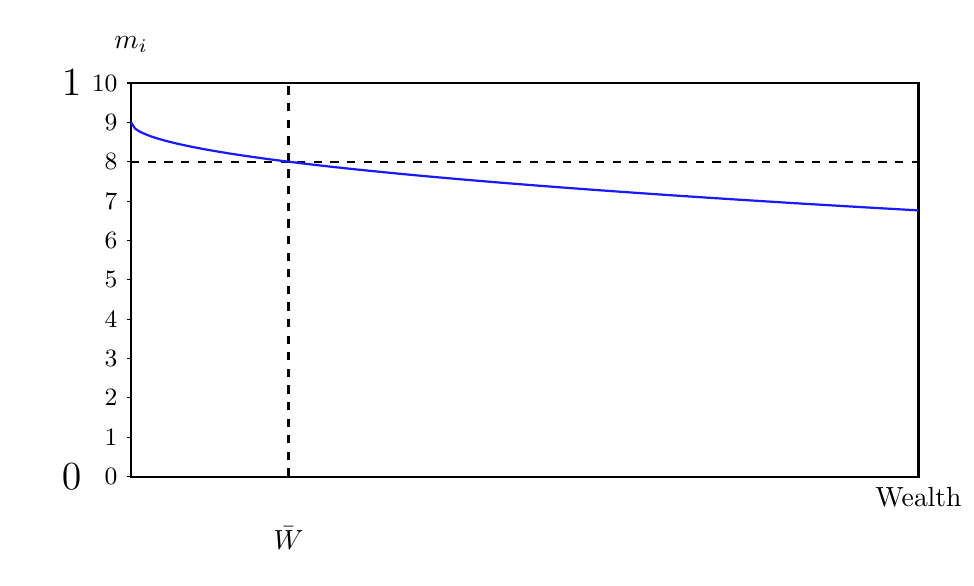
\begin{tikzpicture}[scale=.5]
%\def\bndmax{5}        %https://tex.stackexchange.com/questions/68462/filling-a-complex-region-with-tikz
%\def\bndmin{0.2}
\def\Y{10}  % height of y axis pecent
\def\W{20}  % length  of x axis
\def\Wbar{4}
\def\rbar{8}% this is the prime rate

% %Equation   \[ r_i = (A + .5 \frac{\bar{W}}{W_i})\omega\]
   % \def\Wmin{.63}  %This sets the lower limit fo the 
    \def\Wmin{(\B*\Wbar)/(\Y/\rbar-\A)} %function to keep in in bounds
	
 \tikzset{func/.style={thick,color=blue!90}}	

 \draw [thick](\W,\Y)-- (0,\Y)node[left=.5cm]{\Large$1$}node[above=.25cm]{$m_i$} -- (0,0)node[left=.5cm]{\Large$0$}--(\W,0)node[below]{Wealth}--cycle;  	% Axes box
 
 \draw [dashed, thick] (0,\rbar) -- (\W,\rbar);  	% Axes
\draw [thick,dashed] ( \Wbar,0)node[below=.5cm]{$\bar{W}$} -- (\Wbar,\Y);  	% Axes

\foreach \yi in {0,...,\Y} \draw (0,\yi)--(-.1,\yi)node[left]{\small$\yi$};
%\foreach \yi in {0,2,4,6,8,10} \draw (0,\yi)--(-.1,\yi));
%node[left]{\small$\yi$};
%\foreach \yi in {0,2,4,6,8,10}node at (-.1,yi) {{10*yi}} ;
\draw[func,domain=0:\W] plot [samples=200] (\x,(9-\x^.5/2);

 \end{tikzpicture}
\caption{Individual borrowing ratio $m_i$ as a function of wealth (in tenths)}
 \label{Fig:Borrowingratio}
\end{figure}


\subsection{Individualized borrowing rates}\label{SS:BorowingRate}
 $r_i$ 
 
 $r_i$ should depend on  both the person's income and their assets compared to others. The median after-tax income of Canadian families and unattached individuals was \$66,800 in 2020 according to Statistics Canada's \href{https://www150.statcan.gc.ca/n1/daily-quotidien/220323/dq220323a-eng.htm}{Canadian Income Survey, 2020}.  \href{https://www150.statcan.gc.ca/t1/tbl1/en/tv.action?pid=1110005501}{Data released in 2020 by Statistics Canada} indicates that the top 1\% of Canadians made, on average, around \$512,000 in a single year. \href{https://www150.statcan.gc.ca/n1/daily-quotidien/201222/dq201222b-eng.htm}{Survey of Financial Security, 2019}.

 A study by Statistics Canada found that the typical Canadian household now has a median net worth of \$329,900, while the average net worth in Canada is \$738,200. \href{https://www150.statcan.gc.ca/t1/tbl1/en/tv.action?pid=1110005501}{High income tax filers in Canada}

\subsection{Computing the income constraint on interest rates}\label{SS:YWealthConstraint}
$r_i$

In our model, we  tie the individual cost of capital,  $r_i$ for agent $i$, to a prime rate, $\bar r$ or the bank's target rate, $r^{target}$, prime plus 1\%, say. and to individual wealth. Figures~\ref{Fig:Borrowingrate1} and ref{Fig:Borrowingrate1} illustrate a couple of possible  cost-of-borrowing models roughly consistent  with the stylized facts about lenders. 

\begin{align}
 r_i =  &  \left(A + B \frac{\bar{W}}{W_i}\right) \bar r       \label{eq:incomeandr1}  \\
 r_i =  &  \left(\bar r - A + B *\frac{\bar W}{W_i - C}\right) \label{eq:incomeandr2}  \\
\end{align}
Where $\Bar{W}$ is mean wealth and $W_i$ is individual wealth. In Equation~\ref{eq:incomeandr2},  A determines y-shift, B, the scale, and C the  x-shift for the curve.


\begin{figure}
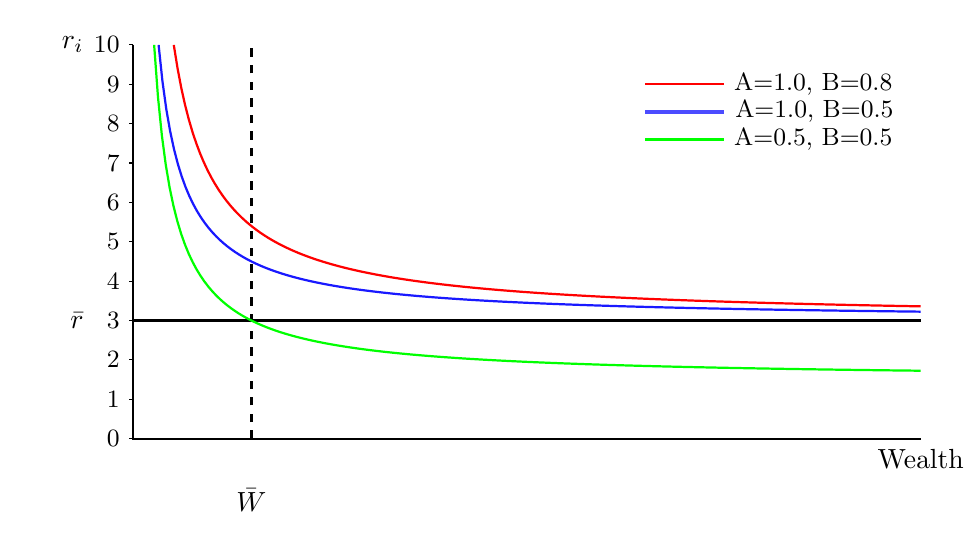
\begin{tikzpicture}[scale=.5]
%\def\bndmax{5} % https://tex.stackexchange.com/questions/68462/filling-a-complex-region-with-tikz
%\def\bndmin{0.2}
\def \Y {10}    % height of y axis as a pecent
\def \W {20}    % length  of x axis
\def \Wbar {3}  % mean wealth
\def \rbar {3}  % the prime rate 

% Equation   \[ r_i = (A + .5 \frac{\bar{W}}{W_i})\omega\]
\def \Wmin{.63}  %This sets the lower limit fo the 
\def \Wmin{(\B*\Wbar)/(\Y/\rbar-\A)} %function to keep in in bounds
\tikzset{func/.style={thick}}	

% Axes
\draw [thick] (0,\Y)node[left=.5cm]{$r_i$} -- (0,0)--(\W,0)node[below]{Wealth};  
\foreach \yi in {0,...,\Y} \draw (0,\yi)--(-.1,\yi)node[left]{\small$\yi$};
\draw [thick] (0,\rbar)node[left=.5cm]{$\bar r$} -- (\W,\rbar);  	% Axes
\draw [thick,dashed] ( \Wbar,0)node[below=.5cm]{$\bar{W}$} -- (\Wbar,\Y);  	% 

\def \A {1.0}  \def \B {0.5} %BLUE
\draw[func,domain=\Wmin:\W, color=blue!90] plot [samples=200] (\x,{(\A+\B*\Wbar/\x)*\rbar});
\draw [ultra thick, color=blue!70 ](13, 8.3)--(15,8.3)node [right, black] {\small A=\A,\ B=\B};

\def \A {0.5} 
\def \B {0.5} % GREEN
\draw[func,domain=\Wmin:\W, color=green] plot [samples=200] (\x,{(\A+\B*\Wbar/\x)*\rbar});
\draw [thick,  color=green](13, 7.6)--(15,7.6)node [right, black] {\small A=\A, B=\B};

\def \A {1.0}  \def \B {0.8} % RED
\draw[func,domain=\Wmin:\W, red] plot [samples=200] (\x,{(\A+\B*\Wbar/\x)*\rbar});
\draw [thick,  color=red](13, 9)--(15,9)node [right, black] {\small A=\A,\ B=\B};
% KEY
\end{tikzpicture}
\caption{Individual borrowing cost as a function of wealth}
\label{Fig:Borrowingrate1}
\end{figure}


\begin{figure}
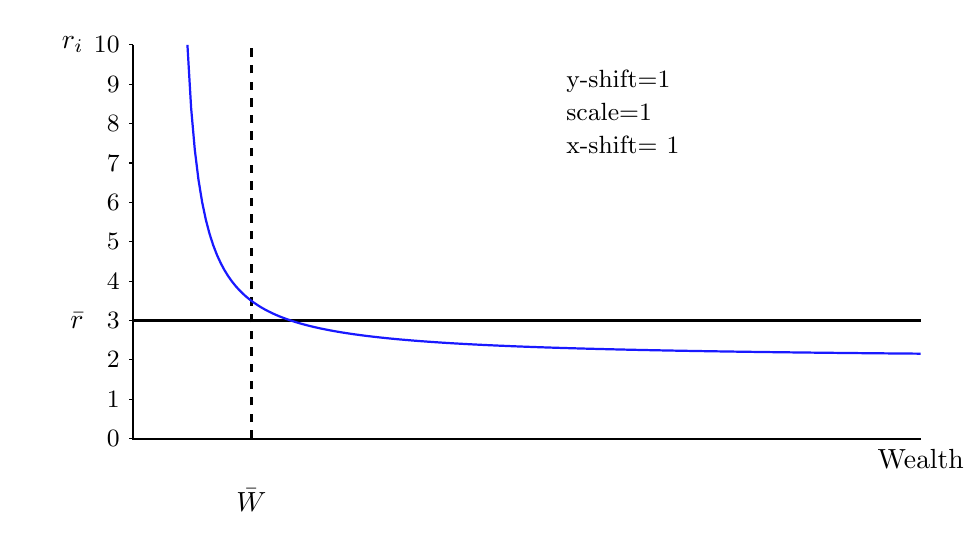
\begin{tikzpicture}[scale=.5]
%\def\bndmax{5}        %https://tex.stackexchange.com/questions/68462/filling-a-complex-region-with-tikz
%\def\bndmin{0.2}
\def \Y {10}  % height of y axis pecent
\def \W {20}  % length  of x axis
\def \Wbar {3} % meam wealth
\def \rbar {3}% this is the prime rate 

%\def \Wmin{(\B*\Wbar)/(\Y/\rbar-\A)} %function to keep in in bounds
\tikzset{func/.style={thick}}	
	% Axes
\draw [thick] (0,\Y)node[left=.5cm]{$r_i$} -- (0,0)--(\W,0)node[below]{Wealth};  
\foreach \yi in {0,...,\Y} \draw (0,\yi)--(-.1,\yi)node[left]{\small$\yi$};
\draw [thick] (0,\rbar)node[left=.5cm]{$\bar r$} -- (\W,\rbar);  	% Axes
\draw [thick,dashed] ( \Wbar,0)node[below=.5cm]{$\bar{W}$} -- (\Wbar,\Y);  	% 

\def \A {1} %vertical shift aroung \rbar, the prime rate
 \def \B {1}  % Scales the exponential curveBLUE
 \def \C {1}  %right shift  
% \def \Wmin {.4+\B}  %This sets the lower limit fo the 
\def \Wmin {(\B*\Wbar)/(\Y-\rbar+\A) +\C} %function to keep in in bounds

\draw[func,domain=\Wmin:\W, color=blue!90] plot [samples=200] (\x,{\rbar-\A+\B*\Wbar/(\x-\C))});
\node  [align=left, text width =2cm ] at (13, 8.3) {\small y-shift=\A \newline scale=\B \newline x-shift= \C};

 \end{tikzpicture}
\caption{Individual borrowing cost as a function of wealth II}
\label{Fig:Borrowingrate2}
\end{figure}

The rates $\delta,\ \sigma,$ and $r$ depend on the period, $T$. 

\section{Incorporating growth and discounting}
%We need a time period T for calculations. For use in any calculation, 

With a price-growth rate of $\dot P$ per year, the growth over $T$ years is $(1+\dot P)^T$, and  %and a 5 year mortgage period, 
the expected price at the end of the period is:

\[P^e_T=P_0(1+\dot P)^T\]

If, for example price growth is 10\%, $\dot P= 0.1$, the {capital gain}, or growth, over a 5-year mortgage term is 0.61051 $\approx$ 60\% of the original price, $P_0$.

If we want the compounded interest rate person $i$ the term T,
\[r_i^T=(1+r_i)^T\]
% This is the value we use in equation~\ref{EqBidPrice}.

If person $i$  discounts at a discount rate $r^\delta$, the present value of a receipt at time $t$ is calculated by using the \textbf{discount factor} $\delta_i^T$.

\[\delta_i^T= \left( \frac{1}{1+r_\delta} \right)^T \]
%\[\delta_i^T= \sum_{\tau=0}^{\tau=T}\left( \frac{1}{1+r_\delta} \right)^\tau \]
 
These can be combined into a function %\delta that  gives a single discounting factor  for a value  like future price that is both growing and being discounted over several (T) periods:
\[ PDV(P^e_T)=P_0\left( \frac{1+\dot P}{1+r_\delta} \right)^T \]
This PDV function specifically combines any expected rent increase, the individual's discount rate and the mortgage term into a single operation.

\subsection{Mortgage availability}
For home loans, many personal finance experts recommend total housing costs account for less than 28\% of your \textbf{gross} household income, This gives us an \textbf{income-based  mortgage maximum} of \[M^{max}_Yi = \frac{0.28*(\omega+w)}{r_i}\] It is the maximum the bank will let you pay.

We assume $r_i$ is based on the individual's assets, on relative wealth. Where is it calculated for the householder or the bank?

We get a \textbf{price-based mortgage maximum} \[M^{max}_P = 0.8P_0\] where $P_0$ is the actual sale price. This is based on the maximum amount of risk that the bank is willing to take on. ($P_0$  will not always be the same as the asking price or the warranted price.)


\section{Table}

\renewcommand{\arraystretch}{1.5}
\begin{tabular}{rlrr}\
Symbol         & Name                                 & Value      & Formula  \\ \hline
$m_i$          & Individual borrowing-ratio           & 0.75-0.85  & $M/P^{ask?}$ \\
$M^{max}_Yi$.  & Maximum mortgage based on income     &            & $\frac{0.28(\omega+w)}{r_i}$ \\
 $M^{max}_P$   & Maximum mortgage based on the price  &            & $0.8*P_0$ \\
$IS$           & Income share for housing debt        & 0.25-0.35  & Missing? \\
$\rho$         & Rent ratio                           &            & $\frac{\omega-tau*d_i}{P_0}$ \\
$\kappa $      & Operations ratio                     & 0.1-0.3    & e.g. $ 0.2\frac{\omega-tau*d_i}{P_0}$ \\
$\sigma$       & Tax ratio                            & 0.25-0.35  & e.g. $ 0.3\frac{\omega-tau*d_i}{P_0}$ \\
$\dot P $      & Price growth                         & []         & $\frac{P_t-P_{t-1}}{P_{t-1}}$\\
$P^T_e$        & Expected price in T years            &            & $P_0(1+\dot P)^T$ \\ % *** WAS $P^e_T$ 
$r_i^\delta$   & Individual discount rate             &            & To assign \\
$\bar r$       & Prime interest rate                  &            & \\
$r_i$          & Individual borrowing-rate            &            & \\
$r^{target}$   & Target interest rate                 &            & $\bar r + margin$ \\
$\delta_i$     & Discount factor for T                &            & $\left(\frac{1}{1+r_i^\delta}\right)^T$ \\
\end{tabular}
\renewcommand{\arraystretch}{1.0}


todo look for $P^e_T$ 

%==========================EXAMPLE=========================== https://www.kaggle.com/code/prateekmaj21/basic-financial-calculations-using-python/notebook
  
% def compound_interest(p,r,t):  %EXAMPLE
    
%     print('Amount: ', p)
%     print("Rate of Interest (Per Annum)", r)
%     print("Time (In Years): ",t)
    
%     a= p*((1+r/100)**t)
    
%     ci= a-p
%     print("Final Amount: ", a)
%     print("Compound Interest: ", ci)
 

\section{Transportation costs}
Transport costs have two parts:
1) fuel and vehicle costs per km
2) time costs per km

\subsection{Vehicle related costs}
Use one year as the wage period, converting transportation costs per km to annual cost for consideration in the household budget. Starting with the cost per km, calculate the cost per year:

\textbf{cost per km =$\textit{t}$}:. \$0.59   (from  Ontario data, 2021). sensitive to congestion, use of subways (\$5 /day?), 

 \textbf{work trips per year} 2 way * 5 days/week * 50 weeks work days = 500. [range: 450-550]

\textbf{cost per km-year} = work trips per year*cost per km

=\$0.59/km*500 trips/year  =  \$295/km year 



\subsection{Time costs}
\textbf{time per km}. range: 20km/hr -> 3min/km, 40km/hr -> (1.5min/km - 3min/ km)per trip 

(New York rush hour is much slower:  4-9km/hr ->6-15 min/km)

\textbf{time  per km-year} = work trips per year*time t per trip = 500* 3min  = 1500 min/km year = 25 hours= 3-3.5 days/km
 
\textbf{time cost per km-year} =  (days per km-year /work days/year)*wage premium per year  = 3/250 = 0.012 years/km year. ?

\textbf{money cost of time per km year} 

=time cost per km-year* wage(including subsistence) 

= 0.012 year* wage per year

\subsection{Total cost per km year of commuting for one agent}
\textbf{money cost of time per km year + \$295/km year * distance} \\
= (0.012 w+ \$295)/km year 
    \begin{quotation}
    \textbf{Example}
    To get a sense of the required wage if we have this annual cost structure, assume city\_extent $d^*$ is 30 km. At this point the transport cost is equal to the wage

\[(0.012 w+ \$295)/km year)*30 =  w\] 
\[.36w+ 8850=w\]
\[w=13828.12\]
        \begin{quotation}
        \textbf{PLAUSIBILITY CHECK}
This is plausible land rent, but does not include building rent. 
Capitalized at 5\% this house is worth \$ 276,562, a fairly cheap house 30 miles from city centre
        \end{quotation}
    \end{quotation}

{\color{red}
\subsection{? Value of $t$ to use in model}}
\[ \tau=(0.012 w+ \$295)/km year \]


\chapter{Amenity}\label{chapter-amenity}

In this chapter, we discuss how amentity might be treated in this model. 
% from Ricardo_Rent_and_Roemer_3.tex
In our base model,  an urban wage premium is the only labour attractor. Transportation costs to the urban center determine land values. Effectively in our base model, we have set the level of amenities to zero  to focus on the productivity effects. The wage premium provides a reason to find housing in the city and to travel to the city centre to work. Housing choice, however, in reality is always the purchase of a bundle of characteristics such as location, building space, yard, local density and local \glsdisp{amenity}{amenities}. Stegman  found that ``a large majority of families who have recently moved to the suburbs are more concerned with neighborhood quality than with accessibility to other parts of the metropolitan region.'' 
``There is evidence that the amenities offered by a city enhance its growth'' \cite{clarkAmenitiesDriveUrban2002, falckPhantomOperaCultural2011} and that amenity effects themselves scale superlinearly \cite{kraemerCulturalSustainabilityUS2022}.

Kaufmann et all \cite{kaufmannScalingUrbanAmenities2022} investigated the general statistical patterns in the quantity and spatial distribution of different urban amenities including public spaces and institutions as well as businesses, which all provide different services to urban populations, such as restaurants, parks, or universities.  They argue that amenities are in fact central for generating and supporting economic agglomeration effects, attracting investment to ``developing neighborhoods, promoting economic growth, supporting innovation clusters and facilitating businesses linkages.'' 
They show that the aggregate quantity of amenity infrastructure (not amenity supply)  in an urban area scales sub-linearly with population size across US metropolitan areas.\footnote{When they disaggregate, however, they find that for approximately 74\% of amenity types, they cannot reject linear scaling. Four percent exhibit super-linear scaling. They list take-away restaurants and travel agents in this range. Sub-linear scaling is associated with libraries, universities, and movie theatres.} This strongly suggests there are scale economies in amenity provision.\footnote{The model they use is the same as the one used to demonstrate that a scaling law holds for urban GDP. Instead of GDP, however, the dependent variable is a measure of amenity density based on data extracted from a unique new Google Places dataset, Google Places API (2012).} 


The amenities offered by a city can be seen as a form of non-market, non-monetary income \cite{kaufmannScalingUrbanAmenities2022}.  The non-market component of household incomes affects choices. Greater consumption amenities in a city will make workers willing to accept lower wages or higher rents. For firms,  lower wages mean lower costs. Thus,  higher amenity levels may lead to lower money wages as workers trade amenity for money income. With lower wages, more workers can be hired leading to higher output and a larger population \cite{pugaMagnitudeCausesAgglomeration2010}. 
When positive urban amenities prevail, rents and housing prices will be higher in larger cities, but wages may be unaffected \cite{robackWagesRentsAmenities1988, dalmazzoAmenitiesSkillbiasedAgglomeration2011}.
%localized productive advantages will make firms willing to accept higher wages and higher rents  


%It involves budget allocation. If we hold the housing budget constant and add an explicit urban amenity, other variables must adjust. 
% Higher wages make residents better off whereas higher rents make them worse off. Thus, 


%.  This helps disentangle the consumption amenities from the productive advantages of big cities.


In our base model,  To introduce amenities we can simply add an amenity value $A$ to the estimated value of any home. The value can depend on location, allowing for `better' and `worse' neighbourhoods,  and it can be made to depend on household attributes: a family with children might value a neighbourhood with a school or a park more highly. 

For some households, the amenity of an area may depend on the density of the city or of certain types in a neighbourhood. This is a social agglomeration effect that may work in addition to the agglomeration effect on production \cite{gurwitzCatastrophicAgglomeration2019} that we have already considered. There are also agglomeration effects in consumption goods. Larger consumer markets support more variety in goods and services. This variety allows a greater range of preferences to be satisfied. A larger city may have more production sectors and a larger array of consumer services, increasing the value received from a given income.  These closely related but different effects can be modeled by introducing an amenity term in various ways 

The amenity-induced rise in housing prices may absorb what would otherwise be consumption expenditure on other goods. Residents might accept smaller housing units for access to urban amenities.\footnote{Some costs may fall with agglomeration. There is evidence of a strong negative correlation between the total energy consumption of a city and its overall urban density \cite{newmanSustainabilityCitiesOvercoming1999}. Larson et al. \cite{larsonEnergyImplicationsCity2015} show that per-capita energy use is relatively invariant to city size when growth is driven by wages but falls modestly with growth induced by rising amenity.} In any case, there will be distributional effects as amenities play a larger role in urban agglomeration. Property owners will capture increased land rents. If amenities are funded out of taxes, the burden falls on all residents, since property taxes are very roughly related to housing consumption, but the land rents are captured by institutional owners as well as owner-occupiers and not by tenants.


%\glspl{amenity}, or non monetary income it another form of wealth,See Kaufmann et al. \cite{kaufmannScalingUrbanAmenities2022}.  and it is %, are however, an important feature of the urban system. 
% We have intentionally suppressed amenity but can add it it simply.
% (ownership effects, produtivity spilllovers, - table where you show them in the static and dynamci case with amentity)
% 2 classes of exploratin of the model in the past tho chaptered

 
%To understand amenity in our model, we need to understand it's relationship with growth, productivity, and agglomeration.
\section{Modelling amenity}

This section sketches an extension of the model to study include \gls{amenity} and suggests how it might affect results. Amenity effects can be introduced in a variety of ways. %hey might work though An economics might prefer to introduce amenity as a good in the utility function of agents.
% It might then depend on the size of the city, the size of an amenity-producing sector, the specific amenity-generating infrastructure provided by the city through taxes,  or neighbourhood effects. Each of these would take a different functional form. In our model agents are represented by their demand for housing, so the same terms would be introduced into the bid function. % In the utility framework, bids are simply derived from the utility function, so the two approaches are equivalent. %  The virtue of using the utility framework is that it begins with the question, ``What do people want?'' rather than ``What do people do?'' The first question is more productive if we want to identify different amenities that might matter.

\subsection{Through household utility}
The most direct way to incorporate agglomeration amenities is  to include what might be called a \gls{utility premium} for urban dwellers as non-monetary location income $\mathbb{A}(d; N), \die{\mathbb{A}}{N}> 0), \die[{\mathbb{A}}]{d}< 0)$ depending on distance, $d$ from the centre and urban population $N$. The second term can incorporate local amenities as well. A simple linear (indirect)\footnote{The indirect utility function is a function that depends on income and prices rather than goods and services.  Income does not generate utility, but it does generate utility indirectly' because it enables people to purchase goods and services.} utility function specified on broad income (net wage plus locational amenity) is convenient for illustration:

\begin{equation}VU(w,A)= \psi+ \omega-cd + \mathbb{A}(d; N) - T(d))
\label{eqn-u}
\end{equation}
where $w$  is an urban wage p, $T(d)$ is transportation cost from the centre to $d$.
\footnote{\cite{anasUrbanSpatialStructure1998} shows that a linear transportation cost will not  hold if congestion declines  with $d$.} 
 In most versions of the Alonzo model the `wage premium' is simply given in the urban wages and there is no amenity term. 


%\footnote{wage income, if all income goes to housing, or the share of wage income going to housing services.   (If we use a Cobb-Douglas utility function we would just replace $w$ with    $\alpha Y$, where $Y$ is household income and $\alpha$ is the share of total income. } Let  $T(d)=td$ be transportation cost with  $t>0$. 
 
\begin{figure}[t!b]
\begin{center}
\begin{tikzpicture}[scale=.5]
\def\bndmax{5}        %https://tex.stackexchange.com/questions/68462/filling-a-complex-region-with-tikz
\def\bndmin{0.2}
\def \n {10}
\def \m {15.5}
\def \t {.5}
\def \th {1}
\def \w {7}
\tikzset{func/.style={thick,color=blue!90}}	
\draw [thick, latex-] (0,\n)node[above] {Rent}--(0,0);
\draw [thick, -latex] (0,0)--(\m,0)node[right=.25]{\large $d$};
%\foreach \xi in {0,..., \m} \draw (\xi,0)--(\xi,-.1)node[below=1]{\small$\xi$};
%\foreach \yi in {1,...,\n} \draw (0,\yi)--(-.1,\yi)node[left]{$\yi$};
%%\foreach \i in {1,4,9,16} {
	\draw[func,domain=0:\m] plot [samples=200] (\x,{\w-\t*\x});
%	\draw[func,domain=0:\m, dashed] plot [samples=200] (\x,{\w+\azero-\th*\x+\aprime*\x});

\node at (14,1.2){$w-T(d)$};
\def \azero{2}
\def \aprime {-.25}	
\tikzset{func/.style={thick,color=orange!90}}	
	\draw[func,domain=0:\m] plot [samples=200] (\x,{\w+\azero-\t*\x+\aprime*\x});
\node at (4,8.5){$w +A(d)-T(d)$};
%\node at(-.8,2) [left]{base $2^1=$};
%\node at(-.8,1) [left]{$2^0=$};
%\draw[dotted] (0,2)--(1,2)--(1,0); 
 \end{tikzpicture}
\end{center}
\caption{Rent profile with amenities}
\label{fig-amenity}
\end{figure}

 This model can produce variations on the standard result in the Alonso model. Figure~\ref{fig-amenity} illustrates a linear amenity function, $\mathbb{A}(d|N)= a-b*d$, that is convenient for illustrative purposes.  It shows how a particular amenity function might affect the rent profile, and hence city size and it allows simple experiments with the effect of increasing population on city size, wages and rents. 

In this case, amenity falls below zero in the outer regions of the city and, the geographical size of the city will be smaller. With a linear function, this happens if $\frac{a}{b} < \frac{w}{t}$. (a smaller city would have a secondary effect on wages, since with fewer workers' marginal productivity would be higher and therefore wages would rise. This would partially offset the initial decline in population.)
There would be a band of land around the city with negative amenity for commuters.\footnote{The very simple graphical result rests on several assumptions - no other housing expense, housing all the same size, wages all equal, preferences identical, transportation costs.}

The far more likely case is that $A(d) > 0$ when $w-T(d)$ falls to zero. In this case there is a band of residents around the city, outside of the population commuting to work. They do not travel to work,  do not collect a wage, but still enjoy the amenity of being close to a city. This might be a population of retired persons enjoying occasional visits and healthcare facilities.


\subsection{Neighbourhood amenity}
In Figure~{fig-amenity} the source of the amenity is at the centre of the city. We can easily imagine an amenity profile that is high for some neigbourhoods and lower for others, as in  In Figure~\ref{fig-amenity2}. The jagged area below the orange line is rent accruing to landowners. The variable rent comes not from a desire to be close to the source of the wage income but from household demand for local amenity.  
\begin{figure}[tb]
\begin{center}
\begin{tikzpicture}[scale=.5]
\def\bndmax{5}        %https://tex.stackexchange.com/questions/68462/filling-a-complex-region-with-tikz
\def\bndmin{0.2}
\def \n {10}
\def \m {15.5}
\def \t {.5}
\def \th {1}
\def \w {7}
\tikzset{func/.style={thick,dashed, color=blue!40}}	
\draw [thick, latex-] (0,\n)node[above] {Rent}--(0,0);
\draw [thick, -latex] (0,0)--(\m,0)node[right=.25]{\large $d$};
% Basic Bid rent,
\node at(-.5,\w) {$\omega$};
\draw[func,domain=0:\m] plot [samples=200] (\x,{\w-\t*\x});
%NEIGBOURHOOD AMENITY
\draw [thick, green] (0,-1)--(2,2)--(4,-1)--(6,2)--(9,0)--(11,1)--(14,0);
\draw [thick, orange] (0,6)--(2,{7-2*.5+2})--(4,7-4*.5 -1)--(6,7-6*.5+2)--(9,7-9*.5)--(11,7-11*.5+1)--(14,7-14*.5);
\node [] at (5,1.3){Neighbourhood amenity};
\def \azero{2}
\def \aprime {-.25}	
% \tikzset{func/.style={thick,color=orange!90}}	
% 	\draw[func,domain=0:\m] plot [samples=200] (\x,{\w+\azero-\t*\x+\aprime*\x});
\node at (4,8.5){$Bid\ rent$};
%\node at(-.8,2) [left]{base $2^1=$};
%\node at(-.8,1) [left]{$2^0=$};
%\draw[dotted] (0,2)--(1,2)--(1,0); 
 \end{tikzpicture}
\end{center}
\caption{Rent profile with neighbourhood amenities}
\label{fig-amenity2}
\end{figure}
Financialization might or might not affect neighbourhood amenity. If it does it might have its effect by changing the ownership mix.

\subsection{Public provision of amenities}

Previous sections suggest amenities may work as a wage subsidy, potentially increasing output. Since employers will not willingly pay for urban amenities, some amenities may be financed publicly. It is common to introduce the cost of generating amenities as a tax on residents.  Since public amenities may be \glspl{public good} in the economic sense, the municipal government may be able to achieve significant wage economies with a small public expenditure.

A simple way to incorporate publicly provided amenities to make an amenity function that proportional to a fraction of public revenue, which is a fraction $\tau$ of the land value when municipalities depend on property taxes. Assuming a uniform property tax rate, total property tax revenue in a circular city are approximately $\tau(\phi+2/3 \omega)\pi \frac{\omega}{c}^2$. We can therefore include in the buyer's maximum bid function a fraction if this value. Property investors would not include this amenity component, but it would affect their decisions because amenity raises their net rent.

Notice that because amenity raises property values, in Ontario it does not raise tax revenue because the property tax rate is adjusted to balance the budget. This creates perverse incentives for municipalities \cite{blaisPerverseCitiesHidden2011}.


\subsection{An amenity sector}
Producing amenities takes resources. Some fraction of the workforce must be engaged in producing the amenity services. A simple approach would be to assume that the base employment that we consider demands a layer of amenities that represent the additional fraction of the population needed to provide the amenities - say 10\%  

Larger cities can support larger and more varied amenities, so that effect of amenities on property values might be larger in larger cities. At the same time, there are apparently economies of scale in the production of amenities \cite{kaufmannScalingUrbanAmenities2022}. We have no strong prior about how in amenity sector would be affected by finacialization of housing.  An effect might work through changing ownership.


\section{Research on amenities}
% There is a great deal of research on amenities. In this subsection mention a few that seemed noteworthy. 
Most of the literature on amenities deals with livability and the benefits for the individual. There is a strand in the literature, however, that links amenities to growth. In 1954, for example, Edward Ullman \cite{ullmanAmenitiesFactorRegional1954} published  ``Amenities as a Factor in Regional Growth,'' an article that came to be seen in the geographical literature over the following 50 years as prescient \cite{walcottCommentsEdwardUllman2010} for introducing the notion that amenities could be an important mobility magnet. 

Many have since extended this approach. Richard Florida, in a series of articles and books beginning in 2002 \cite{floridaCreativeClassEconomic2014, floridaEconomicGeographyTalent2002, floridaCompetingAgeTalent2005} examined the notion that urban growth depended on attracting the creative class and that in turn rested in part on the amenities a city offered. A 2008  Statistics Canada study, `Cities and Growth: The Left Brain of North American Cities,' Beckstead et al \ found substantial differences in average growth for cities with higher cultural employment and urban amenities.  Clark et al \cite{clarkAmenitiesDriveUrban2002} argue that much of Chicago's recent growth to 2003  should be attributed to reforms instituted by Mayor Richard M.  Daley explicitly linked to amenities and quality of life issues, including parks and schools. Abouy \cite{albouyWhatAreCities2016} finds that wage and housing cost differences across metropolitan areas are accounted for more by productivity than quality-of-life differences, however. 

Beckstead et al  \cite{becksteadCitiesGrowthLeft2008} identify amenities with the unexplained variastion in median urban house price after controlling for median household income.\footnote{  The basic premise would be that after conditioning on household income, variation in home prices across cities would be a function of the relative attractiveness of these places. The residuals yield a continuous ranking of cities based on the estimated variation in urban amenities.} Rappaport \cite{rappaportConsumptionAmenitiesCity2008} presents empirical evidence that amenities do support high-density levels, and that amenities cause approximately one-fifth of the cross-sectional variation in metro population density. 


% Molotch's (1976) metaphor suggests that the city is a machine geared to creating growth, with growth loosely defined as the intensification of land use and thus higher rent collections associated professional fees and locally based profits. Many urban economists, planners, and political scientists have made similar arguments (e.g., Bradbury, Downs, & Small, 1982; Mollenkopf, 1983; Stone, 1989). However, a quarter century later in the contemporary competition among US cities, the growth machine model has lost much of its power.
  


\newpage


\chapter{Notation}
% \section{Notation for Urban and Production Sectors}
\newpage
\begin{longtable}{lp{10cm}}
\caption{Notation}                       \\
\hline           &  \textbf{Productivity} \\ \hline
$K$              &  Capital               \\ 
% $L$            &  Labour                \\
$N$              &  Population, equals labour \\ %, $L$          
%$\Lambda$    &  Labour-augmenting agglomeration effect \\
$Y=A K^{\alpha }N^{\beta }$  &  a Cobb-Douglas Production function \\ %Urban output            \\
$\alpha$         &  Elasticity of output with respect to capital          \\
$\beta$          &  Elasticity of output with respect to labour           \\ % vs effective labour
$\gamma$         &  Elasticity of agglomeration with respect to labour    \\ % , $\Lambda(n)$, for illustration \\

% $L$              &  Labour supply \\ %the number of workers, which, in the standard circular city model, equals the number of lots of size $s$  when workers live on identical individual lots. % Unless $d^{max}>d^*$ v  \frac{\pi}{s}(\frac{w}{{c}})^2 =
$n$  &  Number of workers at a firm \\
% $n_i$  &  Number of workers employed by firm $i$ \\
%$n=\sum_i n_i$  &  Number of workers, the urban population in the model \\
% $\#f=\frac{n}{n_i}$&number of identical firms \\ %not used
% $f$  &  Number of firms =1 \\
% $n =f n_i$  &  Aggregate labour \\
% $n^\gamma$ & The labour-augmenting agglomeration effect,  modelled as an exponential function of the number of people \\
% $\Lambda(n)n_i$ &  Effective labour for firm $i$ \\
% $\Lambda'=\die{\Lambda(n)}{n} $ & Derivative of the labour-augmenting agglomeration effect\\

%%$Y_i=K_i^{\alpha }(\Lambda(n)n_i)^{\beta }$  &  Urban firm $i$'s output \\

%%$Y=\frac{n}{n_i}K_i^{\alpha }(\Lambda(\sum_i n_i)n_i)^{\beta }$  &  Aggregate output of all firms in the city \\
% $\die{Y}{n}=\beta\frac{1}{n} Y  \left( 1+ \frac{n\Lambda'}{\Lambda} \right)$  &  Social marginal product of labour \\
% $Y_i=K_i^{\alpha }(\Lambda(n)n_i)^{\beta }$    &  Urban firm $i$'s output \\
% $\die{Y_i}{K_i}	=\alpha \frac{1}{K_i} Y_i $  & Marginal product of capital for firm $i$ \\
% $\die{Y_i}{n_i}	=  \beta\frac{1}{n_i} Y_i $  &  Marginal product of labour for firm $i$ \\
%%$\eta=\frac{n_i\Lambda'}{\Lambda}$  &   Marginal agglomeration effect on a firm's output of increasing it's own labour stock \\
% \hline
	% &\textbf{Amenity}\\ \hline
% $A(d, n)$   &  Agglomeration amenity          \\

\hline  0 &  \textbf{Labour market}                \\ \hline %and urban stucture??
$\psi$            &  Rural subsistence wage                             \\  
$\omega$          &  Urban wage premium          \\
${c}$             &  Transportation cost per unit distance \\ % Was $\tau$, and $trans$. Considered $\gamma, \xi, \zeta$.
$d$               &  Distance from city centre   \\
$d^* = w/{c}$     &  City extent \\ %, the maximum distance commuters will travel \\ % Maximum distance commuters will travel \\ % to get the wage premium \\
% $\mathcal{R} = \omega - {dc}$ &  Rent at distance ${d}$ \\ 
% $\zeta$          &  Population density at distance $d$     \\
% $s$              &  Lot size      \\
% $\psi$  &  ?Per-period cost of a unit of productive capital \\
% $\omega + \psi$  &  Urban wage including rural wage \\ %***
% $\textit{t}$ & {\color{red}transportation cost per km} \\%use   c?
% $w^n=\omega-{dc}$ & Wage  premium net of transportation costs \\
%% $\Omega=\frac{\omega+\psi}{\psi}$  &  Ratio of the urban wage to the  cost of capital \\
%% $\Pi$	   &  Profit \\
%% $ER$	   &  Excess return to capital \\ 
% \hline &\textbf{Spatial structure in the circular city} \\ \hline		
%% $d^{max} = \omega /{c}$  &  Maximum distance commuters at which residents enjoy the urban amenity \\
%% $d^{**} = max(d^*, d^{max})$  &  radius of the city \\
%% $U$                     &  Worker utility **\\ %, a function of location and prices \\
%% $U^{urban}=U^{rural} $  &  Migration equilibrium assumption ** \\
% \hline & \textbf{Labour market} \\ 

\hline           & \textbf{Financial market}             \\ \hline
$P_W$            &  Warranted price for a property       \\
$P_B$            &  Bid price                            \\ % was P^{bid}
$P_A$            &  Asking price                         \\
$P_M$            &  Realized market price                \\
$P_M^e$          &  Expected market price                \\
% $P$            &  Price of a property                  \\ 
% $\dot P$       &  Rate of price growth              \\ % was $\dot p$  
% $\mathcal{C}$    &  Capital gains                     \\ % was C
% $\mathcal{C}_N$  &  Net capital gain, $C -$ net rent  \\
% $M$              &  Mortgage                          \\ 
% $m$              &  Mortgage share, the share of the property price that can be borrowed, which is a function of wealth  \\ 
$\mathcal{R}$    &  Rent                              \\
$\mathcal{R}_N$  &  Net rent                          \\
${R}^w_N$        &  Warranted rent                    \\
$\rho$           &  Rent ratio                        \\
$\phi$           &  \Gls{rent share}                  \\
$\mathcal{O}$    &  Operational costs                 \\
% $\theta$         &  Operations ratio                  \\ % was $\kappa$ became b
$\mathcal{T}$    &  Taxes                             \\ % was $\Sigma, \Xi$  
$\tau$           &  Property tax share                \\ % was t then $\sigma, \xi$  b
% $\tau$            &  Annual tax rate on rent and home \\ % Was $c$ 
$r$              &  Interest rate                     \\
$\delta$         &  Individual's subjective \gls{discount factor} \\
% $W$            &  Wealth                            \\
% $\psi$         &  Fraction with rent/operating costs\\
$t$              &  Time                              \\

W & Wealth \\
m & Mortgage share \\
M & Mortgage \\
S & Savings \\
% \mathbb{C} carrying 0.28, max_mortgage share, wealth_sensitivity

$\mathbb{T}$     &  Time period                       \\

$a$       &  Share of subsistence wage  used for land and building \\
$b$       &  Maintenance share of share of subsistence wage \\ % A cost. Includes water, electricity, heat? 
% $wage_share$     & OLD Share of the agglomeration effect that goes to workers. \\

\hline
\color{black}
\end{longtable}  

\newpage

\begin{longtable}{lp{10cm}}
\caption{Rent}                                                            \\
\hline
$\omega-{dc}$                &  Warranted (economic) rent                \\
$\mathcal{R}=\omega-{dc}$    &  Equilibrium rent payment of tenant       \\
PDV                           &  Present discounted value                 \\  
$\mathcal{R}^T$               &  PDV of rent collected over period $T$    \\ 
$\mathcal{R}^T_N=(1-\kappa-\sigma)\mathcal{R}^T$  &  PDV of net rent collected over period $T$ \\
\hline
\end{longtable}

\begin{longtable}{lp{10cm}}
\caption{Bidding mechanism notation}                                          \\
\hline
$\mathcal{R}_N$  &  Net rent                                                  \\ % was NR
% $P_0$            &  Purchase price for a property                             \\
% $P^T_e$          &  Expected price at the end of period $T$                   \\
$r^{prime}$         &  Prime interest rate                                       \\
$r^{target}$     &  Investor or banks target interest rate, $\bar r + margin$ \\

$r_i$            &  Agent $i$'s personal borrowing rate                       \\
$r_i^T$          &  Agent $i$ interest rate compounded over a period $T$      \\
$r_i^{disc}$     &  Agent $i$'s subjective discount rate (which may equal $r_i$) \\
$r_\delta$       &  Discount rate                                             \\ % was $discr_i$
$\delta_i^T$     &  Discount factor for agent $i$ over period $T$             \\
$m^W$            &  Wealth-based share of home price a worker can mortgage    \\ % $= m_i(W_i)$
$m^\omega$       &  Income-based share of home price a worker can mortgage    \\ % IS_i   IS_i(\omega+\psi)$$
$m_i = min(m^W_i, m^\omega_i)$  & Mortgage, the share of home price worker $i$ can mortgage \\

\hline
\color{black}
\end{longtable}  
Notation: 
Agent counts and indices are subscripts.
Values related to time are superscripts, time as a continuous 
variable is small, a period is capitalized e.g. the period $T$ of some number of years. 
In general values are capitals, rates are small letters.

% It might be better to use the subscript $m$ for `market'.  for warranted rents



 


% GLOSSARIES (Lists of definitions, abbreviations, symbols, etc. provided by the glossaries-extra package)
% -----------------------------
\printglossary
\cleardoublepage
\phantomsection		% allows hyperref to link to the correct page

%----------------------------------------------------------------------
\end{document} % end of logical document